%!TeX program = XeLaTex
%!TEX encoding = UTF-8 Unicode

\documentclass[10pt,twoside]{book}
\XeTeXlinebreaklocale "my_MM"  %Myanmar line and character breaks
\XeTeXinterwordspaceshaping=2

\usepackage[
    paperheight = 10.2in,
    paperwidth = 7.4in,
    right = 0.8in,
    left = 1.45in,
    top = 0.75in,
    bottom = 0.9in,
    heightrounded,
    asymmetric,
    %showframe
]{geometry}
\usepackage[parfill,indent=2em,skip=3pt plus 1pt]{parskip}

\usepackage[no-math]{fontspec}
\usepackage{stmaryrd}

%\SetSymbolFont{largesymbols}{bold}{OMX}{txex}{b}{n}
\usepackage{titletoc}
\usepackage{titlesec}
\usepackage{fancyhdr}
\usepackage[bookmarksnumbered,hidelinks]{hyperref}
\usepackage{bookmark}
\makeatletter
\renewcommand\Hy@numberline[1]{(#1) } 
\makeatother


\usepackage[dvipsnames,table]{xcolor}
\usepackage{booktabs}
\usepackage{multirow}
\usepackage{array}
\newcommand{\rowsep}{\arrayrulecolor{black!30}\midrule[0.25pt]\arrayrulecolor{black}}
\usepackage{siunitx}

\usepackage{caption}
\usepackage[labelformat=simple]{subcaption}
%\renewcommand\thesubfigure{\alph{subfigure}}

\usepackage[outputdir=out]{minted}
\usepackage{pifont}

\usepackage{amsmath}
\usepackage{amssymb}
\usepackage{mathtools}
%\usemintedstyle{bw}


\usepackage{multicol}

\usepackage{graphicx}
\usepackage{subcaption}
\usepackage{tikz}
\usetikzlibrary{tikzmark}
\usetikzlibrary {shapes.symbols} 
\usepackage{forest}
\usetikzlibrary{shadows}


\usetikzlibrary{decorations.pathreplacing,calligraphy}
\usepackage{onimage}
\usetikzlibrary{arrows.meta}
\usepackage{adjustbox}
%https://tex.stackexchange.com/questions/9796/how-to-add-todo-notes
\usepackage[textcolor=blue,
    textsize=scriptsize,
    textwidth=17.5mm,
    color=red!25,
    disable]{todonotes}

\definecolor{boxfillcolor}{RGB}{242,242,242}
\definecolor{boxfillcolor2}{RGB}{232,232,232}


%\newcommand{\mintrule}{0.0pt}
%\newcommand{\mintsep}{5pt}
%\newcommand{\mintframe}{lines}
%\newcommand{\xlftmargin}{2pt}
%\definecolor{mintbgcolor}{RGB}{251, 251, 249}
%\definecolor{mintrulecolor}{RGB}{190,190,190}

\newcommand{\mintrule}{0.5pt}
\newcommand{\mintsep}{2pt}
\newcommand{\mintframe}{leftline}
\newcommand{\xlftmargin}{0pt}
\definecolor{mintbgcolor}{RGB}{255, 255, 255}
\definecolor{mintrulecolor}{RGB}{190,190,190}
% control vspace between two minted env
%\AfterEndEnvironment{minted}{\par\vspace{-\baselineskip}}
\newcommand{\betweenminted}[1]{%
\par\vspace{-\medskipamount}\vspace{-0.5\baselineskip}%
\vspace{#1}%
}

\BeforeBeginEnvironment{minted}{\vspace{0.5\baselineskip}}
\AfterEndEnvironment{minted}{\vspace{0.5\baselineskip}}


\newcommand{\btwntikzannoandpar}{%
\vspace{-1.33518\baselineskip}%
}%


\newcommand{\betweentcboxpar}{%
\par\vspace{0.75em}%
}

\usepackage[most]{tcolorbox}
\newtcolorbox{mytcbox}{
    left=3pt,right=3pt,top=3pt,bottom=3pt,
    colframe=lightgray,
    boxrule=0.4pt,
    colback=boxfillcolor,
    before upper={\parindent0em}
}


\newtcolorbox{mytcboxflt}{
    left=3pt,right=3pt,top=3pt,bottom=3pt,
    float=htb,
    colframe=gray,
    boxrule=0.4pt,
    colback=boxfillcolor,
    before upper={\parindent0em}
}

\newtcbox{\mytcboxinl}[1][boxfillcolor2]{
    on line,
    arc=1.5pt,colback=#1,colframe=#1!50!black,
    before upper={\rule[-3pt]{0pt}{10pt}},
    boxrule=0pt,
    boxsep=0pt,left=1pt,right=1pt,top=1.25pt,bottom=.7pt
}

    
\usepackage{afterpage}
\newcommand\blankpage{%
    \null
    \thispagestyle{empty}%
    \addtocounter{page}{-1}%
    \newpage}

\usepackage{appendix}
\renewcommand\appendixname{နောက်ဆက်တွဲ}
\renewcommand\appendixpagename{နောက်ဆက်တွဲ}



\AtBeginEnvironment{py}{\let\special\pyspecial} 
\def\pyspecial{\kern0pt\primitive\special}
\makeatletter
\AtBeginEnvironment{py}{\dontdofcolorbox}
\def\dontdofcolorbox{\renewcommand\fcolorbox[4][]{##4}}
\makeatother

\AtBeginEnvironment{pytc}{\let\special\pytcspecial} 
\def\pytcspecial{\kern0pt\primitive\special}
\makeatletter
\AtBeginEnvironment{pytc}{\dontdofcolorbox}
\def\dontdofcolorbox{\renewcommand\fcolorbox[4][]{##4}}
\makeatother

\AtBeginEnvironment{codetxt}{\let\special\codetxtspecial} 
\def\codetxtspecial{\kern0pt\primitive\special}
\makeatletter
\AtBeginEnvironment{codetxt}{\dontdofcolorbox}
\def\dontdofcolorbox{\renewcommand\fcolorbox[4][]{##4}}
\makeatother


\newcommand{\bropn}{\{}

\setminted[java]{fontfamily=IBMPlexMonoFamily}
\setminted[text]{fontfamily=IBMPlexMonoFamily}
\setminted[python]{fontfamily=IBMPlexMonoFamily}

\AtBeginEnvironment{minted}{\let\special\mintedspecial} 
\def\mintedspecial{\kern0pt\primitive\special}
\makeatletter
\AtBeginEnvironment{minted}{\dontdofcolorbox}
\def\dontdofcolorbox{\renewcommand\fcolorbox[4][]{##4}}
\makeatother
\setminted{baselinestretch=1.12}
\usepackage{environ}
\newenvironment{py}
{\VerbatimEnvironment
\begin{minted}[
    frame=\mintframe, 
    framerule=\mintrule,
    framesep= \mintsep, 
    xleftmargin=\xlftmargin, 
    bgcolor=mintbgcolor,
    rulecolor=mintrulecolor,
    python3=true
    ,escapeinside=ßß]{python}}
 {\end{minted}}

 \newenvironment{pytc}
{\VerbatimEnvironment
\begin{minted}[
    frame=\mintframe, 
    framerule=\mintrule,
    framesep= \mintsep, 
    xleftmargin=\xlftmargin, 
    bgcolor=boxfillcolor,
    rulecolor=mintrulecolor,
    python3=true
    ,escapeinside=ßß]{python}}
 {\end{minted}}

\newenvironment{codetxt}
{\VerbatimEnvironment
\begin{minted}[
    frame=\mintframe, 
    framerule=\mintrule,
    framesep= \mintsep, 
    xleftmargin=\xlftmargin, 
    bgcolor=mintbgcolor,
    rulecolor=mintrulecolor
    ,escapeinside=ßß]{text}}
 {\end{minted}}
\defaultfontfeatures[Padauk Book]{}
\setmainfont[
    Path = fonts/,
    UprightFont = PadaukBook-Regular.ttf,
    BoldFont = PadaukBook-Bold.ttf,
    ItalicFont = PadaukBook-Regular.ttf,    
]{Padauk Book}
[Renderer = Graphite, RawFeature = {Tear drop style washwe=True}]

\newfontfamily{\padaukfamily}{Padauk Book}[
    Path = fonts/,
    UprightFont = PadaukBook-Regular.ttf,
    BoldFont = PadaukBook-Bold.ttf,
    ItalicFont = PadaukBook-Regular.ttf,
    Renderer=OpenType]
\DeclareTextFontCommand{\textpadauk}{\padaukfamily}

\newfontfamily{\jetbrainsmonofamily}{JetBrainsMonoNL}[
    Path = fonts/jetbrains_mono/,
    Scale = 0.80,
    UprightFont=*-Regular.ttf,
    ItalicFont=*-Italic.ttf,
    BoldFont=*-Bold.ttf,
    SmallCapsFont=*-Regular.ttf,
    BoldItalicFont=*-BoldItalic.ttf,
    NFSSFamily=JetBrainsMonoFamily]
\DeclareTextFontCommand{\textjetbrainsmono}{\jetbrainsmonofamily}

\newfontfamily{\ibmplexmonofamily}{IBMPlexMono}[
    Path = fonts/ibm_plex_mono/,
    Scale = 0.84,
    UprightFont=*-Text.ttf,
    ItalicFont=*-TextItalic.ttf,
    BoldFont=*-Bold.ttf,
    SmallCapsFont=*-Regular.ttf,
    BoldItalicFont=*-BoldItalic.ttf,
    HyphenChar=None,
    NFSSFamily=IBMPlexMonoFamily]
\DeclareTextFontCommand{\textibmplexmono}{\ibmplexmonofamily}
\newfontfamily{\ibmplexmonofamilya}{IBMPlexMono}[
    Path = fonts/ibm_plex_mono/,
    UprightFont=*-Text.ttf,
    ItalicFont=*-TextItalic.ttf,
    BoldFont=*-SemiBold.ttf,
    SmallCapsFont=*-Regular.ttf,
    BoldItalicFont=*-SemiBoldItalic.ttf]
\DeclareTextFontCommand{\textibmplexmonoa}{\ibmplexmonofamilya}

\newfontfamily{\ibmplexsansfamily}{IBMPlexSans}[
    Path = fonts/ibm_plex_sans/,
    Scale = 1,
    UprightFont=*-Text.ttf,
    ItalicFont=*-TextItalic.ttf,
    BoldFont=*-Bold.ttf,
    SmallCapsFont=*-Regular.ttf,
    BoldItalicFont=*-BoldItalic.ttf,
    HyphenChar=None]
\DeclareTextFontCommand{\textibmplexsans}{\ibmplexsansfamily}

\newfontfamily{\ibmplexseriffamily}{IBMPlexSerif}[
    Path = fonts/ibm_plex_serif/,
    Scale = 1,
    UprightFont=*-Text.ttf,
    ItalicFont=*-TextItalic.ttf,
    BoldFont=*-Bold.ttf,
    SmallCapsFont=*-Regular.ttf,
    BoldItalicFont=*-BoldItalic.ttf,
    HyphenChar=None]
\DeclareTextFontCommand{\textibmplexserif}{\ibmplexseriffamily}

%
\newfontfamily{\latinmodernfamily}{lmroman10}[
    Path = fonts/latin_modern/,
    Extension = .otf,
    UprightFont = *-regular, 
    BoldFont = *-bold,
    ItalicFont = *-italic,
    BoldItalicFont = *-bolditalic,
    SmallCapsFont = lmromancaps10-regular
]
\DeclareTextFontCommand{\textlatinmodern}{\latinmodernfamily}

% downloaded from https://notofonts.github.io/myanmar/ 
\newfontfamily{\notoserifmmfamily}{Noto Serif Myanmar SemiCondensed}[
    Path=fonts/noto_serif_mm/,
    UprightFont=NotoSerifMyanmar-SemiCondensedLight.ttf,
    ItalicFont = NotoSerifMyanmar-SemiCondensedLight.ttf,
    BoldItalicFont = NotoSerifMyanmar-SemiCondensedMedium.ttf,
    BoldFont=NotoSerifMyanmar-SemiCondensedMedium.ttf, Script=Myanmar]
\DeclareTextFontCommand{\textnotoserifmm}{\notoserifmmfamily}


% for normal paragraphs
\NewDocumentCommand{\fEn}{m}{%
    \textlatinmodern{\addfontfeatures{Scale=MatchLowercase}#1}%
}
\NewDocumentCommand{\fEnBf}{m}{%
    \textlatinmodern{\bfseries\addfontfeatures{Scale=MatchLowercase}{#1}}%
}
\NewDocumentCommand{\fEnEmp}{m}{%
    \textlatinmodern{\itshape #1}%
}

\NewDocumentCommand{\fEnEmpBf}{m}{%
    \textlatinmodern{\bfseries\itshape #1}%
}

% for page numbers on each page
\newfontfamily{\padaukbook}{Padauk Book}[
        Path = fonts/,
        UprightFont = PadaukBook-Regular.ttf,
        BoldFont = PadaukBook-Bold.ttf, Renderer = Graphite, RawFeature = {Tear drop style washwe=True}]
\DeclareTextFontCommand{\textpadaukbook}{\padaukbook}
\NewDocumentCommand{\fPageNo}{m}{%
    \textpadaukbook{%
        \addfontfeatures{Mapping = mmdigit_mapping} #1}%
}
\NewDocumentCommand{\fMM}{m}{%
    \textpadaukbook{%
        \addfontfeatures{Scale=0.9,FakeSlant=0.22} #1}%
}

\NewDocumentCommand{\fMMSm}{m}{%
    \textpadaukbook{%
        \addfontfeatures{Scale=0.94} #1}%
}

%=========================================================================================
% Chapter Title
\NewDocumentCommand{\fChNo}{m}{%
    \begingroup%
    \textnotoserifmm{\addfontfeatures{FakeSlant=0.25, Mapping = mmletter_digit_mapping}#1}%
    \endgroup%
}

\NewDocumentCommand{\fCh}{m}{%
    \begingroup%
    \textnotoserifmm{\addfontfeatures{FakeSlant=0.25}#1}%
    \endgroup%
}

% for section and subsection
\NewDocumentCommand{\fSec}{m}{%
    \begingroup%
    \textnotoserifmm{%
    \addfontfeatures{}%
    #1%
    }%
    \endgroup%
}

\NewDocumentCommand{\fSubSec}{m}{%
    \begingroup%
    \textnotoserifmm{%
    \addfontfeatures{}%
    #1%
    }%
    \endgroup%
}

\NewDocumentCommand{\fSecNo}{m}{%
    \begingroup%
    \textnotoserifmm{%
    \addfontfeatures{Mapping = mmletter_digit_mapping}%
    #1%
    }%
    \endgroup%
}

\NewDocumentCommand{\fCpt}{m}{%
    \begingroup%
    \textnotoserifmm{%
    \addfontfeatures{Scale=0.9}%
    #1%
    }%
    \endgroup%
}

\NewDocumentCommand{\fCptNo}{m}{%
    \begingroup%
    \textnotoserifmm{%
    \addfontfeatures{Mapping = mmletter_digit_mapping,Scale=0.9}%
    #1%
    }%
    \endgroup%
}

\NewDocumentCommand{\fSecCode}{m}{%
    \begingroup%
    \textibmplexmonoa{%
    \addfontfeatures{Scale=1}%
    #1%
    }%
    \endgroup%
}

\NewDocumentCommand{\fChCode}{m}{%
    \begingroup%
    \itshape\textibmplexmonoa{%
    \addfontfeatures{Scale=1}%
    #1%
    }%
    \endgroup%
}

\NewDocumentCommand{\fCode}{m}{%
    \begingroup%
    \textibmplexmono{#1}%
    \endgroup%
}
\NewDocumentCommand{\fCodeBf}{m}{%
    \begingroup%
    \bfseries\textibmplexmono{#1}%
    \endgroup%
}%
\NewDocumentCommand{\fSecCodeBf}{m}{%
    \begingroup%
    \textibmplexmonoa{%
    \bfseries\addfontfeatures{Scale=1}%
    #1%
    }%
    \endgroup%
}
\NewDocumentCommand{\fSubSecCodeBf}{m}{%
    \begingroup%
    \textibmplexmonoa{%
    \bfseries\addfontfeatures{}%
    #1%
    }%
    \endgroup%
}
\NewDocumentCommand{\fCptCodeBf}{m}{%
    \begingroup%
    \textibmplexmonoa{%
    \bfseries\addfontfeatures{Scale=MatchLowercase}%
    #1%
    }%
    \endgroup%
}

\NewDocumentCommand{\fRefNo}{m}{%
    \begingroup%
    \textpadaukbook{%
    \addfontfeatures{Mapping = mmletter_digit_mapping}%
    #1%
    }%
    \endgroup%
}

\NewDocumentCommand{\fOpn}{m}{%
    \begingroup%
    \textpadauk{%
    \addfontfeatures{Renderer=OpenType}%
    #1%
    }%
    \endgroup%
}

% for table head
\NewDocumentCommand{\fTblHead}{m}{%
    \begingroup%
    \bfseries\textnotoserifmm{%
    \addfontfeatures{Scale=MatchLowercase}%
    #1%
    }%
    \endgroup%
}

\NewDocumentCommand{\fCoverTitle}{m}{%
    \begingroup%
    \textibmplexserif{%
    \Huge\addfontfeatures{Color=PythonYellow,Scale=7}%
    #1%
    }%
    \endgroup%
}

\NewDocumentCommand{\fCoverTitleII}{m}{%
    \begingroup%
    \textibmplexsans{%
    \Huge\addfontfeatures{Color=White, Scale=1.4}%
    #1%
    }%
    \endgroup%
}

\NewDocumentCommand{\fEnSnd}{m}{%
    \begingroup%
    \textibmplexserif{%
    \addfontfeatures{Scale=MatchLowercase}%
    #1%
    }%
    \endgroup%
}

\NewDocumentCommand{\fFBTtl}{m}{%
    \begingroup%
    \textibmplexsans{%
    \Huge\addfontfeatures{Color=PythonYellow,Scale=7}%
    #1%
    }%
    \endgroup%
}



\renewcommand{\thechapter}{\arabic{chapter}}
\renewcommand{\chaptername}{အခန်း}

\setlength{\headheight}{14pt}

\titleformat{\chapter}[display]
    {\bfseries\Huge}
    {\fCh{\chaptertitlename}\ \fChNo{\thechapter}} % အခန်း ၁
    {20pt}
    {\Large\fCh} % အခန်းခေါင်းစဉ်

\titleformat{\section}
    {\bfseries\large}
    {\fSecNo\thesection}
    {8pt}
    {\bfseries\fSec}

\titleformat{\subsection}
    {\bfseries}
    {\fSecNo\thesubsection}
    {8pt}
    {\bfseries\fSubSec}

\fancypagestyle{plain}{% plain style is used by pages where new chapter begins
    \fancyhf{}% clear all header and footer fields
    \fancyfoot[C]{\bfseries\fPageNo\thepage}% have page no at the btm for chapter start
}

\fancypagestyle{fancy}{%
    \fancyhf{} % clear all header and footer fields
    \fancyhead[LO,RE]{\bfseries\fPageNo\thepage}
    %\fancyhead[RE]{\leftmark}
    %\fancyhead[LO]{\rightmark}
    \renewcommand{\headrulewidth}{0pt}
    \renewcommand{\footrulewidth}{0pt}
}

\fancypagestyle{fancyfront}{%
    \fancyhf{} % clear all header and footer fields
    \fancyhead[LO,RE]{\bfseries\fEn{\thepage}}
    %\fancyhead[RE]{\leftmark}
    %\fancyhead[LO]{\rightmark}
    \renewcommand{\headrulewidth}{0pt}
    \renewcommand{\footrulewidth}{0pt}
}

\fancypagestyle{plainfront}{% plain style is used by pages where new chapter begins
    \fancyhf{}% clear all header and footer fields
    \fancyfoot[C]{\bfseries\fEn{\thepage}}% have page no at the btm for chapter start
}
\usetikzlibrary{shadows,calc}
% some parameters for customization
\def\shadowshift{1.5pt,-1.5pt}
\def\shadowradius{4pt}
\colorlet{innercolor}{black!50}
\colorlet{outercolor}{gray!5}
% this draws a shadow under a rectangle node
\newcommand\drawshadow[1]{
\begin{pgfonlayer}{shadow}
    \shade[outercolor,inner color=innercolor,outer color=outercolor] ($(#1.south west)+(\shadowshift)+(\shadowradius/2,\shadowradius/2)$) circle (\shadowradius);
    \shade[outercolor,inner color=innercolor,outer color=outercolor] ($(#1.north west)+(\shadowshift)+(\shadowradius/2,-\shadowradius/2)$) circle (\shadowradius);
    \shade[outercolor,inner color=innercolor,outer color=outercolor] ($(#1.south east)+(\shadowshift)+(-\shadowradius/2,\shadowradius/2)$) circle (\shadowradius);
    \shade[outercolor,inner color=innercolor,outer color=outercolor] ($(#1.north east)+(\shadowshift)+(-\shadowradius/2,-\shadowradius/2)$) circle (\shadowradius);
    \shade[top color=innercolor,bottom color=outercolor] ($(#1.south west)+(\shadowshift)+(\shadowradius/2,-\shadowradius/2)$) rectangle ($(#1.south east)+(\shadowshift)+(-\shadowradius/2,\shadowradius/2)$);
    \shade[left color=innercolor,right color=outercolor] ($(#1.south east)+(\shadowshift)+(-\shadowradius/2,\shadowradius/2)$) rectangle ($(#1.north east)+(\shadowshift)+(\shadowradius/2,-\shadowradius/2)$);
    \shade[bottom color=innercolor,top color=outercolor] ($(#1.north west)+(\shadowshift)+(\shadowradius/2,-\shadowradius/2)$) rectangle ($(#1.north east)+(\shadowshift)+(-\shadowradius/2,\shadowradius/2)$);
    \shade[outercolor,right color=innercolor,left color=outercolor] ($(#1.south west)+(\shadowshift)+(-\shadowradius/2,\shadowradius/2)$) rectangle ($(#1.north west)+(\shadowshift)+(\shadowradius/2,-\shadowradius/2)$);
    \shade[outercolor,right color=innercolor,left color=innercolor] ($(#1.north west)+(-\shadowradius/12,\shadowradius/12)$) rectangle ($(#1.south east)+(\shadowradius/12,-\shadowradius/12)$);%Frame
    \filldraw ($(#1.south west)+(\shadowshift)+(\shadowradius/2,\shadowradius/2)$) rectangle ($(#1.north east)+(\shadowshift)-(\shadowradius/2,\shadowradius/2)$);
\end{pgfonlayer}
}
% create a shadow layer, so that we don't need to worry about overdrawing other things
\pgfdeclarelayer{shadow} 
\pgfsetlayers{shadow,main}
% Define image shadow command
\newcommand\shadowimage[2][]{%
\begin{tikzpicture}
\node[anchor=south west,inner sep=0] (image) at (0,0) {\includegraphics[#1]{#2}};
\drawshadow{image}
\end{tikzpicture}}
\renewcommand{\figurename}{ပုံ}
\renewcommand{\tablename}{တေဘဲလ်}
\DeclareCaptionFont{cptfont}{\notoserifmmfamily\addfontfeatures{Scale=0.9}}


% Separator style using colon, dash, etc
% to get "Figure (1):", "Figure(1) - Some caption" etc
\DeclareCaptionLabelSeparator{cptSep}{\quad}

% to get "Figure (1)", "Figure [1]", etc, set to labelformat below
% #1 is Figure, #2 is the figure number 1.1, 1,2, etc
\DeclareCaptionLabelFormat{cptFmt}
    {{\bfseries\fCpt{#1}} {\bfseries\fCptNo{#2}}}

\DeclareCaptionLabelFormat{subCptFmt}
    {{\bfseries\fCptNo{(#2)}}}


\captionsetup[figure]
{
    labelformat=cptFmt,
    singlelinecheck=false,
    margin=0pt,
    justification=raggedright,
    labelsep=cptSep,
    %font={cptfont,bf} % both
    %labelfont={cptfont, bf}, % affect label num and sep 
    textfont={cptfont, bf} % affect only caption title   
}

\captionsetup[subfigure]
{
    labelformat=subCptFmt,
    singlelinecheck=false,
    margin=0pt,
    justification=raggedright,
    labelsep=cptSep,
    %font={cptfont,bf} % both
    %labelfont={cptfont, bf}, % affect label num and sep 
    textfont={cptfont, bf} % affect only caption title   
}

\captionsetup[table]
{
    labelformat=cptFmt,
    singlelinecheck=false,
    margin=0pt,
    justification=raggedright,
    labelsep=cptSep,
    %font={cptfont,bf} % both
    %labelfont={cptfont, bf}, % affect label num and sep 
    textfont={cptfont, bf} % affect only caption title   
}
%\renewcommand{\labelitemi}{\normalfont\ding{239}}
%\renewcommand{\labelitemi}{\color{myItmiColor}\RIGHTarrow}
\let\oldding\ding% Store old \ding in \oldding
\renewcommand{\ding}[2][1]{\scalebox{#1}{\oldding{#2}}}% Scale \oldding via optional argument
\renewcommand{\labelitemi}{\ding[0.6]{110}}

\renewcommand{\labelitemii}{\ding[0.85]{229}}
\renewcommand{\labelitemiii}{\ding[0.85]{229}}
%\renewcommand{\labelitemiii}{\tiny\ding{110}}
\renewcommand{\labelitemiv}{\tiny\ding{110}}
\renewcommand{\contentsname}{မာတိကာ} 
\contentsmargin[0cm]{0cm} % right edge -1cm from the margin, left edge same as left margin

%\newbool{numbered}
%\titlecontents{part}[0em]{\large\sffamily\protect\addvspace{15pt}}%
%{\global\booltrue{numbered}\contentslabel[{\partname\enspace\thecontentslabel}]{0em}\brlap[1.25\baselineskip]}%{\global\boolfalse{numbered}}%
%{\ifbool{numbered}{\hphantom{\partname\ \thecontentslabel\enspace}}{}\titlerule\contentspage}%

\titlecontents{chapter}[0pt]
{\addvspace{4pt}\bfseries\large}
% can only use font family
{\let\fSecCodeBf\fCodeBf\notoserifmmfamilytoc\addfontfeatures{Color=darkgray}\contentslabel[\notoserifmmfamilytoc\addfontfeatures{Mapping=mmletter_digit_mapping,Color=darkgray}{\thecontentslabel}]{20pt}}
{0pt}%
{\hfill\notoserifmmfamilytoc\addfontfeatures{Mapping=mmletter_digit_mapping, Color=darkgray}{\contentspage}}[\vskip 6pt]

\titlecontents{section}[25pt] % move both section number and title name
{}
% can only use font family
{\let\fSecCodeBf\fCodeBf\notoserifmmfamilytoc\addfontfeatures{Scale=MatchLowercase, Color=darkgray}\contentslabel[\notoserifmmfamilytoc\addfontfeatures{Mapping=mmletter_digit_mapping,Scale=MatchLowercase, Color=darkgray}{\thecontentslabel}]{25pt}}
{0pt}%
{{\titlerule*[.5pc]{\color{gray}{.}}} \notoserifmmfamilytoc\addfontfeatures{Mapping=mmletter_digit_mapping,Scale=MatchLowercase,Color=darkgray}{\contentspage}}[\vskip 4pt]








\begin{document}
\pagestyle{empty}
\definecolor{PythonBlue}{RGB}{67, 110, 155}
\definecolor{PythonYellow}{RGB}{250, 224, 117}

\begin{tikzpicture}[remember picture,overlay] 

\node[rectangle,
    draw=PythonBlue,
    text = White,
    fill = PythonBlue, 
    minimum width = 7.4in, 
    minimum height = 10.2in, anchor=west]
    at (current page.west) 
    {};  
\node[left, black, anchor=north west] at (-3, 1)
    {\fCoverTitleII{Begin Modern Programming}};
\node[left, black, anchor=north west] at (-3, -1)
    {\fCoverTitleII{with}};
\node[left, black, rotate=90] at (11, -1)
    {\fCoverTitle{Python}};
\node[left, black, anchor=west] at (-3,-22)
    {\fCoverTitleII{Pyi Soe}};
\end{tikzpicture}
\pagestyle{fancyfront}
\pagenumbering{roman}
\tableofcontents
\addtocontents{toc}{\protect\thispagestyle{plainfront}}


%\pagestyle{empty}
\definecolor{PythonBlue}{RGB}{67, 110, 155}
\definecolor{PythonYellow}{RGB}{250, 224, 117}

\begin{tikzpicture}[remember picture,overlay] 

\node[rectangle,
    draw=PythonBlue,
    text = White,
    fill = PythonBlue, 
    minimum width = 7.4in, 
    minimum height = 10.2in, anchor=west]
    at (current page.west) 
    {};  

\node[left, black, rotate=90] at (5.5, -1)
    {\fFBTtl{MP\textit{w}P}};

\end{tikzpicture}
%\pagestyle{empty}
\definecolor{PythonBlue}{RGB}{67, 110, 155}
\definecolor{PythonYellow}{RGB}{250, 224, 117}

\begin{tikzpicture}[remember picture,overlay] 

\node[rectangle,
    draw=PythonBlue,
    text = White,
    fill = PythonBlue, 
    minimum width = 7.4in, 
    minimum height = 10.2in, anchor=west]
    at (current page.west) 
    {};  

\node[left, black, rotate=90] at (0, -1)  
    {\fCoverTitleII{Begin Modern Programming with}};
\node[left, black, rotate=90] at (4, 2)
    {\fFBTtl{Python}};

\end{tikzpicture}
\pdfstringdefDisableCommands{%fSecCodeKw
  \def\\{}%
  \def\fSecCodeBf#1{#1}%
  \def\fSubSecCodeBf#1{#1}%
}

\mainmatter
\pagenumbering{arabic}
\pagestyle{fancy}
\chapter{စက်ရုပ်ကားရဲလ်ဖြင့် ပရိုဂရမ်းမင်းမိတ်ဆက်} \label{ch:ch01}
ကွန်ပျူတာတွေဟာ သက်မဲ့ စက်ပစ္စည်းတွေပါပဲ။ ကားတို့၊ လေယာဉ်တို့နဲ့ မတူတာက ကွန်ပျူတာတွေဟာ စက်ချည်းသက်သက် ဘာအစွမ်းမှ မယ်မယ်ရရ မရှိဘူး။ ဒါပေမဲ့ ဆောင်ရွက်လိုတဲ့ ကိစ္စအဝဝအတွက် ပရိုဂရမ်အမျိုးမျိုး ထည့်ပေးလိုက်တဲ့အခါမှာ သူ့ရဲ့အစွမ်းက အတိုင်းအဆမဲ့ပဲ။ နေရာမျိုးစုံ၊ နယ်ပါယ်မျိုးစုံမှာ အကူအညီပေးနိုင်တဲ့ စွယ်စုံသုံး ပစ္စည်းတစ်ခုဖြစ်သွားတယ်။ ဂီတသံစဉ်တွေကို ဖွင့်ပေးနိုင်သလို အသံလည်းသွင်းပေးနိုင်တယ်။ ရုပ်ရှင်တည်းဖြတ် လုပ်ချင်တာလား။ ပြဿနာမရှိဘူး၊ ကူညီပေးနိုင်တယ်။ နျူကလီး\allowbreak ယား ဓါတ်ပေါင်းဖိုတွေကို စီမံနိုင်သလို မောင်းသူမဲ့ ဒုံးပျံတွေကိုလည်း ပဲ့ထိန်းပေးနိုင်တယ်။ 

ကျွန်တော်တို့တွေ နိစ္စဓူဝ အသုံးပြုနေကြတဲ့ ကား၊ စမတ်ဖုန်း၊ လက်ပါတ်နာရီ၊ မိုက်ခရိုဝေဖ့်မီးဖို၊ အဝတ်လျှော်စက် စတဲ့ စက်ပစ္စည်း အမျိုးမျိုးဟာလည်း ကွန်ပျူတာတွေနဲ့ မကင်းပြန်ပါဘူး။ “ကွန်ပျူတာနည်းပညာ အကူအညီမပါတဲ့ ခေတ်မီဆန်းသစ်တီထွင်မှုဆိုတာ မရှိဘူး” လို့ ဆိုနိုင်ပါတယ်။

တစ်ချက်တစ်ချက် ရိုက်ခတ်လိုက်တဲ့ ကွန်ပျူတာနည်းပညာ လှိုင်းလုံးကြီးတွေဟာ ကမ္ဘာတစ်ဝှမ်းလုံး ပုံစံပြောင်းသွားလောက်အောင် အဟုန်ပြင်းထန်လှတယ်။ ဘီလီယံနဲ့ချီတဲ့ လူတွေ ဆိုရှယ်မီဒီယာတွေပေါ်ကနေ ရုပ်သံတွေနဲ့ ချိတ်ဆက်ပြောဆိုဆက်သွယ်လို့ ရစေတာဟာလည်း ကွန်ပျူတာစနစ်တွေပါပဲ။ \fEn{Artificial Intelligence (AI)} နည်းပညာကြောင့် သက်ရှိတွေမှာပဲတွေ့ရတဲ့ ညာဏ်ရည်မျိုးကို ကွန်ပျူတာတွေမှာလည်း တွေ့လာရပါပြီ။ သင်္ချာပုစ္ဆာတွေ ဖြေရှင်းခြင်း၊ စစ်တုရင်ထိုးခြင်း စတဲ့ကိစ္စမျိုးတွေအပြင် ပန်းချီဆွဲခြင်း၊ ကဗျာရေးစပ်ခြင်း၊ သီချင်းရေးဖွဲ့ခြင်း ကဲ့သို့ အနုပညာဖန်တီးမှုတွေကိုပါ \fEn{AI} က လုပ်ဆောင်ပေးနိုင်ပါတယ်။ နှစ်ဆယ့်တစ်ရာစုရဲ့ အထူးခြားဆုံး \fEn{AI} နည်းပညာလှိုင်းဟာ အရှိန်အဟုန်ပြင်းပြင်း ရိုတ်ခတ်ဖို့ အားယူစ ပြုနေပါပြီ။

‘ကွန်ပျူတာ’ လို့ပြောတဲ့အခါ စက်ပစ္စည်းသက်သက် မဟုတ်ဘဲ ကွန်ပျူတာမှတ်ညာဏ်ထဲက ပရိုဂရမ်တွေလည်း ပါဝင်တယ်ဆိုတာ သတိချပ်ရပါမယ်။ ကွန်ပျူတာတွေ တစ်စုံတစ်ရာ စွမ်းဆောင်နိုင်စေတဲ့  ပရိုဂရမ်တွေ ရေးတဲ့အလုပ်ကို ပရိုဂရမ်းမင်း\fEn{(Programming)} လို့ခေါ်တယ်။

\section{စက်ရုပ် ကားရဲလ်}
% ====================
ပရိုဂရမ်းမင်းဆိုတာ ဘယ်လိုမျိုးလဲ သဘောပေါက်အောင် စာတွေတစ်သီကြီးရေး ရှင်းပြတာထက် ပရိုဂရမ်လေးတွေ လက်တွေ့ ရေးကြည့်လိုက်တာ ပိုပြီးထိရောက်ပါတယ်။ ဒါကြောင့် စက်ရုပ်ကားရဲလ်ကို ပရိုဂရမ်လေးတွေရေးပြီး အလုပ်တွေခိုင်းကြည့်ကြမယ်။ ပုံ (\fRefNo{\ref{fig:meet_karel_1}}) မှာ တွေ့ရတာက ကားရဲလ် ရောက်ရှိနေတဲ့ နမူနာ ကမ္ဘာတစ်ခုပါ။ မီးခိုးရောင် မှန်ကူကွက်ပုံလေးကို ဘိပါ \fEn{(beeper)} လို့ ခေါ်တယ်။ အဲဒီဘိပါကို မြှားပြထားတဲ့ နေရာကို ရွှေ့ခိုင်းချင်တယ်။ မျဉ်းမည်းအထူတွေက နံရံတွေပါ။
%
\begin{figure}[htb!]
\begin{tikzonimage}[width=4in]{images/ch_a_programming_with_karel/meet_karel.jpg} %, tsx/show help lines]
    \draw[-{Latex[length=3mm]}] (0.7 ,0.8)--(0.645, 0.635);
\end{tikzonimage}
\caption{စက်ရုပ်လေး ကားရဲလ်}
\label{fig:meet_karel_1}
\end{figure}
%
ကားရဲလ်ကို ကိစ္စတစ်ခု ဆောင်ရွက်စေချင်တဲ့အခါ အခြေခံ ကားရဲလ်ကွန်မန်းတွေကို အသုံးပြုရပါတယ်။ ကွန်မန်းတွေကို နှုတ်နဲ့ပြောပြီး ခိုင်းရတာမဟုတ်ဘဲ ပရိုဂရမ်ရေးပြီး ခိုင်းရတာပါ။ ကားရဲလ်နားလည်တဲ့ ကွန်မန်းတွေကို ကြည့်ကြရအောင်။
%
\subsection*{ကားရဲလ်ကွန်မန်းများ}
% ==========================
မဖြစ်မနေ သိထားရမဲ့ အခြေခံ ကားရဲလ်ကွန်မန်း လေးခုပဲ ရှိတယ်။ \fCode{move}\fEn{,} \fCode{turn\_left}\fEn{,} \fCode{put\_beeper} နဲ့ \fCode{pick\_beeper}\ တို့ဖြစ်တယ်။ အခြား ကားရဲလ်ကွန်မန်း တွေလည်း ရှိပါသေးတယ်။ ဒါပေမဲ့ ကားရဲလ် ပရိုဂရမ်းမင်း စလေ့လာဖို့ ဒီလေးခုနဲ့ပဲ လုံလောက်ပါပြီ။

\fCode{move} ကွန်မန်းက ကားရဲလ်ကို ရှေ့တစ်ကွန်နာကို ရွှေ့ခိုင်းတာ။ ကားရဲလ်ကမ္ဘာထဲမှာ တစ်ခုနဲ့တစ်ခု အကွာအဝေးတူ ခြားထားတဲ့ အတန်းလိုက် အတန်းလိုက် အစက်ကလေးတွေဟာ ကွန်နာ \fEn{(corner)} တွေ ဖြစ်တယ်။ ကမ္ဘာကို မျဉ်းမည်းအထူ နံရံတွေနဲ့ ထောင့်မှန်စတုဂံပုံ ပါတ်လည် ဘောင်ခတ်ထားတယ်။ ကွန်နာတွေကြားမှာလည်း နံရံတွေရှိနိုင်တယ်။ နမူနာကမ္ဘာမှာ ဘေးတိုက် နံပါတ်စဉ် ၄ နဲ့ ၅ ကြား ထောင်လိုက် နံရံတစ်ခု၊ အထက်အောက် နံပါတ်စဉ် ၂ နဲ့ ၃ ကြား အလျားလိုက် နံရံတစ်ခုကို တွေ့ရပါမယ်။ ကွန်နာရှေ့မှာ နံရံကာနေရင် ကားရဲလ်ကို \fCode{move} ခိုင်းလို့မရပါဘူး။ 

\fCode{put\_beeper}\ က ကားရဲလ် လက်ရှိ ရှိနေတဲ့ ကွန်နာမှာ ‘ဘိပါတစ်ခုချ’ ထားခိုင်းတာ၊ \fCode{pick\_beeper}\ က ရပ်နေတဲ့ ကွန်နာမှာ ‘ဘိပါတစ်ခုကောက်’ ခိုင်းတာပါ။ ကွန်နာမှာ ဘိပါရှိနေမှ ကောက်ခိုင်းလို့ရမှာပါ။ မရှိရင် ကောက်ခိုင်းလို့ မရဘူး။ ဘိပါချခိုင်းရင်လည်း ကားရဲလ်မှာ ဘိပါရှိမှ ချခိုင်းလို့ရတယ်။ ကားရဲလ်ကို ဘိပါတွေ လိုသလောက် ဖြည့်ပေးထားတယ်လို့ ယူဆပါ။  \fCode{turn\_left} က ‘ဘယ်လှည့်’ ခိုင်းတာ။ \todo{ကမ္ဘာအသစ်တည်ဆောက်ရင် ဘိပါအရေအတွက် လိုသလိုဖြည့်ထားလို့ရကြောင်း ရှင်းပြဖို့လိုမလား}

\subsection*{ဘိပါကို ဘယ်လိုရွှေ့ခိုင်းမလဲ}
% ================================
ပုံ (\fRefNo{\ref{fig:meet_karel_1}}) အနေအထားကနေ ရှေ့ကို သုံးနေရာရွှေ့၊ ဘိပါကောက်၊ ဘယ်ဘက်လှည့်၊ အပေါ် နှစ်နေရာရွှေ့၊ ညာဘက်လှည့်၊ ရှေ့တစ်နေရာထပ်ရွှေ့ပြီး ဘိပါချထားခိုင်းလိုက်ရင် အလုပ်ပြီးသွားပါပြီ။

ကားရဲလ်ကို ညာဘက်လှည့်ခိုင်းဖို့ \fCode{turn\_right} ကွန်မန်း မရှိဘူး။ ဒါပေမဲ့ ဘယ်သုံးခါလှည့်တာဟာ ညာဘက်လှည့်တာနဲ့ တူတူပါပဲ။ ဒါကြောင့် ညာဘက်ချင်တဲ့အခါ ဘယ်သုံးခါလှည့်ခိုင်းလို့ရတယ်။

\section{Meet Karel ပရိုဂရမ်}
ပရိုဂရမ် ရေးတယ်ဆိုတာ ကွန်ပျူတာကို ကိစ္စတစ်ခုခု ဆောက်ရွက်ပေးဖို့ ခိုင်းစေတဲ့  ညွှန်ကြားချက်တွေ ရေးတာပါပဲ။ ဒီလို ညွှန်ကြားချက်တွေကို ပရိုဂရမ်ကုဒ် \fEn{(program code)} လို့ ခေါ်တယ်။ ပရိုဂရမ်ကုဒ်တွေကို ကွန်ပျူတာနားလည်တဲ့ \fEn{programming language} တစ်ခုခုနဲ့ ရေးရတယ်။ ဒီစာအုပ်မှာ အသုံးပြုမဲ့ \fEn{programming language} ကတော့ \fEn{Python} ပါ။ \fEn{Programming language} တစ်မျိုးပဲ ရှိတာမဟုတ်ပါဘူး။ ရာနဲ့ချီပြီး ရှိတာပါ။ လူ့ဘာသာစကားတွေ အမျိုးမျိုးရှိသလိုပဲပေါ့။ \fEn{Python} ဟာ ဒီလို ရာနဲ့ချီတဲ့ထဲက လက်ရှိအသုံးအများဆုံး ထိပ်ဆုံးဆယ်ခု ထဲမှာ ပါဝင်တယ်။ \fEn{Python} နဲ့ ဘိပါရွှေ့ခိုင်းတဲ့ ပရိုဂရမ်ကို လေ့လာကြည့်ရအောင်။ ကားရဲလ်နဲ့ ပထမဆုံး မိတ်ဆက်ပေးတဲ့ ပရိုဂရမ်မို့လို့ ဒီပရိုဂရမ် နံမည်ကို \fEn{‘Meet Karel’} လို့ ခေါ်ပါမယ်။
%
\setlength{\fboxsep}{0pt}
\begin{minted}[frame=\mintframe, framerule=\mintrule,framesep= \mintsep, xleftmargin=\xlftmargin
    , bgcolor=mintbgcolor,rulecolor=mintrulecolor
    , python3=true,escapeinside=ßß]{python}
# File: meet_karel.py
# About: This is
from stanfordkarel import *


def main():
    """Karel code goes here!"""
    move()
    move()
    move()
    pick_beeper()
    turn_left()
    move()
    move()

    turn_left()
    turn_left()
    turn_left()

    move()
    put_beeper()
# End of main

if __name__ == "__main__":
    run_karel_program("meet_karel")

\end{minted}
%

ဒါဟာ \fEn{‘Meet Karel’} ပရိုဂရမ်အတွက် \fEn{Python} နဲ့ရေးထားတဲ့ ပရိုဂရမ်ကုဒ် တွေဖြစ်ပါတယ်။ ‘\fEn{Python} ကုဒ်’ လို့ အတိုချုံးပဲ ပြောတာများတယ်။ \fEn{Python} ‘စာ/စကား’ မတတ်ရင် ဒီ ‘\fEn{Python} ကုဒ်’ တွေကိုလည်း နားလည်မှာ မဟုတ်ဘူး။ ဒီတော့ \fEn{Python} ‘စာ/စကား’ အခြေခံက စပြီး လေ့လာဖို့ လိုပါမယ်။
\todo{စာ ကို footnote ထည့်ရန်}

\subsection*{ကွန်းမန့် (Comment)}
ပထမဆုံး \fCode{\textit{\#}} သင်္ကေတနဲ့ စတဲ့ စာကြောင်းတွေက ကွန်းမန့်တွေပါ။ ကွန်းမန့်တွေက ကွန်ပျူတာ ဆောင်ရွက်ပေးရမဲ့ ညွှန်ကြားချက်တွေ မဟုတ်ဘူး။ ပရိုဂရမ်ကုဒ်နဲ့ ပါတ်သက်ပြီး ကုဒ် ဖတ်ရှူသူ အတွက် မှတ်ချက်ရေးတာ သို့မဟုတ် ရှင်းပြထားတာပါ။ တနည်းအားဖြင့် ဖတ်ရှုသူ (လူ) ပရိုဂရမ်မာအတွက် ရည်ရွယ်တာ။ ကွန်ပျူတာ (စက်) အတွက် ရည်ရွယ်တာ မဟုတ်ဘူး။ ကွန်ပျူတာက ကုဒ်ထဲက ကွန်းမန့်တွေ အားလုံးကို လစ်လျူရှုမှာပါ။ ဒါပေမဲ့ ပရိုဂရမ်ကုဒ်ကို ဖတ်တဲ့လူ နားလည်ဖို့ အထောက်အကူ ဖြစ်စေတဲ့အတွက် ကွန်းမန့်ရေးတာကို ပေါ့ပေါ့တန်တန် အရေးမပါသလို သဘောထားလို့ မရပါဘူး။ မိမိရေးတဲ့ ကုဒ်ကို ရှင်းပြဖို့ လိုအပ်ရင် ကွန်းမန့်ရေးရပါမယ်။ ရေးသင့်တဲ့ နေရာတွေကိုလည်း မကြာခင်တွေ့ရမှာပါ။

\subsection*{\fSubSecCodeBf{import} စတိတ်မန့်}
%
\setlength{\fboxsep}{0pt}
\begin{minted}[frame=\mintframe, framerule=\mintrule,framesep= \mintsep, xleftmargin=\xlftmargin
    , bgcolor=mintbgcolor,rulecolor=mintrulecolor
    , python3=true,escapeinside=ßß]{python}
from stanfordkarel import *
\end{minted}
%
ကတော့ အင်ပို့စတိတ်မန့် ဖြစ်ပါတယ်။ “\fCode{stanfordkarel} လိုက်ဘရီမှ အာလုံးကို ထည့်သွင်းပေးပါ” လို့ တောင်းဆိုတဲ့ အဓိပ္ပါယ်။ \fCode{*} သင်္ကေတကို ‘အားလုံး’ လို့ ယူဆပါ။  \fCode{stanfordkarel} လိုက်ဘရီမှာ ကားရဲလ်ပရိုဂရမ်အတွက် လိုအပ်တာအားလုံး   ပါဝင်တယ်။  ဒီလိုက်ဘရီကို အင်ပို့လုပ်ထားမှ ကားရဲလ်ကွန်မန်းတွေ သုံးလို့ရမှာပါ။ သီးခြား ကားရဲလ်ပရိုဂရမ် တစ်ခုစီတိုင်းအတွက် အင်ပို့လုပ်ရမှာ ဖြစ်တယ်။

\subsection*{လိုက်ဘရီ}
လိုက်ဘရီ \fEn{(\fEnEmpBf{library})} ဆိုတာ ပညာရပ်နယ်ပယ် တစ်ခုအတွက် ရည်ရွယ်ရေးထားတဲ့ ပရိုဂရမ်ကုဒ်တွေပါပဲ။ သင်္ချာအတွက်အချက် လိုက်ဘရီ၊ ဂိမ်းရေးဖို့ လိုက်ဘရီ၊ \fEn{2D/3D} ဂရပ်ဖစ်ဆွဲဖို့ လိုက်ဘရီ၊ အေအိုင်အတွက် လိုက်ဘရီ စသည်ဖြင့် နယ်ပယ်အသီးသီး၊ ကိစ္စရပ်အဖုံဖုံအတွက် သက်ဆိုင်ရာ ကျွမ်းကျင်ပညာရှင်တွေ ထုတ်လုပ်ဖြန့်ချီပေးထားတဲ့ လိုက်ဘရီတွေရှိတယ်။ \fEn{Matrix} အော်ပရေးရှင်းတွေအတွက် \fCode{numpy} ၊ ဂရပ်ဖ်ဆွဲမယ်ဆိုရင် \fCode{matplotlib} စတဲ့ လိုက်ဘရီတွေကို အင်ပို့လုပ် အသုံးပြုနိုင်ပါတယ်။ မေ့ထရစ် $A$ ကို $B$ နဲ့ မြှောက်ရင် ဒီလိုပါ 
%
\setlength{\fboxsep}{0pt}
\begin{minted}[frame=\mintframe, framerule=\mintrule,framesep= \mintsep, xleftmargin=\xlftmargin
    , bgcolor=mintbgcolor,rulecolor=mintrulecolor
    , python3=true,escapeinside=ßß]{python}
from numpy import *

A = array([[1, 1, 2, 2],
           [2, 2, 1, 1],
           [2, 2, 1, 1]])
B = array([[2, 2],
           [2, 2],
           [1, 1],
           [2, 2]])

result = matmul(A, B)

print(result)

\end{minted}
%
ရလဒ် အခုလိုထွက်ပါမယ်။ 
%
\begin{minted}[frame=lines, framerule=0pt]{text}
[[10 10]
 [11 11]
 [11 11]]
\end{minted}
%
ဒါကတော့ ဘားချတ် အတွက် \fCode{numpy} နဲ့ \fCode{matplotlib} လိုက်ဘရီ သုံးထားတာပါ။  
%
\setlength{\fboxsep}{0pt}
\begin{minted}[frame=\mintframe, framerule=\mintrule,framesep= \mintsep, xleftmargin=\xlftmargin
    , bgcolor=mintbgcolor,rulecolor=mintrulecolor
    , python3=true,escapeinside=ßß]{python}
from matplotlib.pyplot import *
from numpy import *

# make data:
x = 0.5 + arange(8)
y = [4.8, 5.5, 3.5, 4.6, 6.5, 6.6, 2.6, 3.0]

# plot
fig, ax = subplots()
bar(x, y, width=1, edgecolor="white", linewidth=0.7)

ax.set(xlim=(0, 8), xticks=arange(1, 8),
       ylim=(0, 8), yticks=arange(1, 8))

show()
\end{minted}
ဘားချတ်ကို ဒီလို ထုတ်ပေးပါတယ်။
%
\begin{figure}[tbh!]
\begin{tikzpicture}
    \node[anchor=south west,inner sep=0] (image) at (0,0)
        {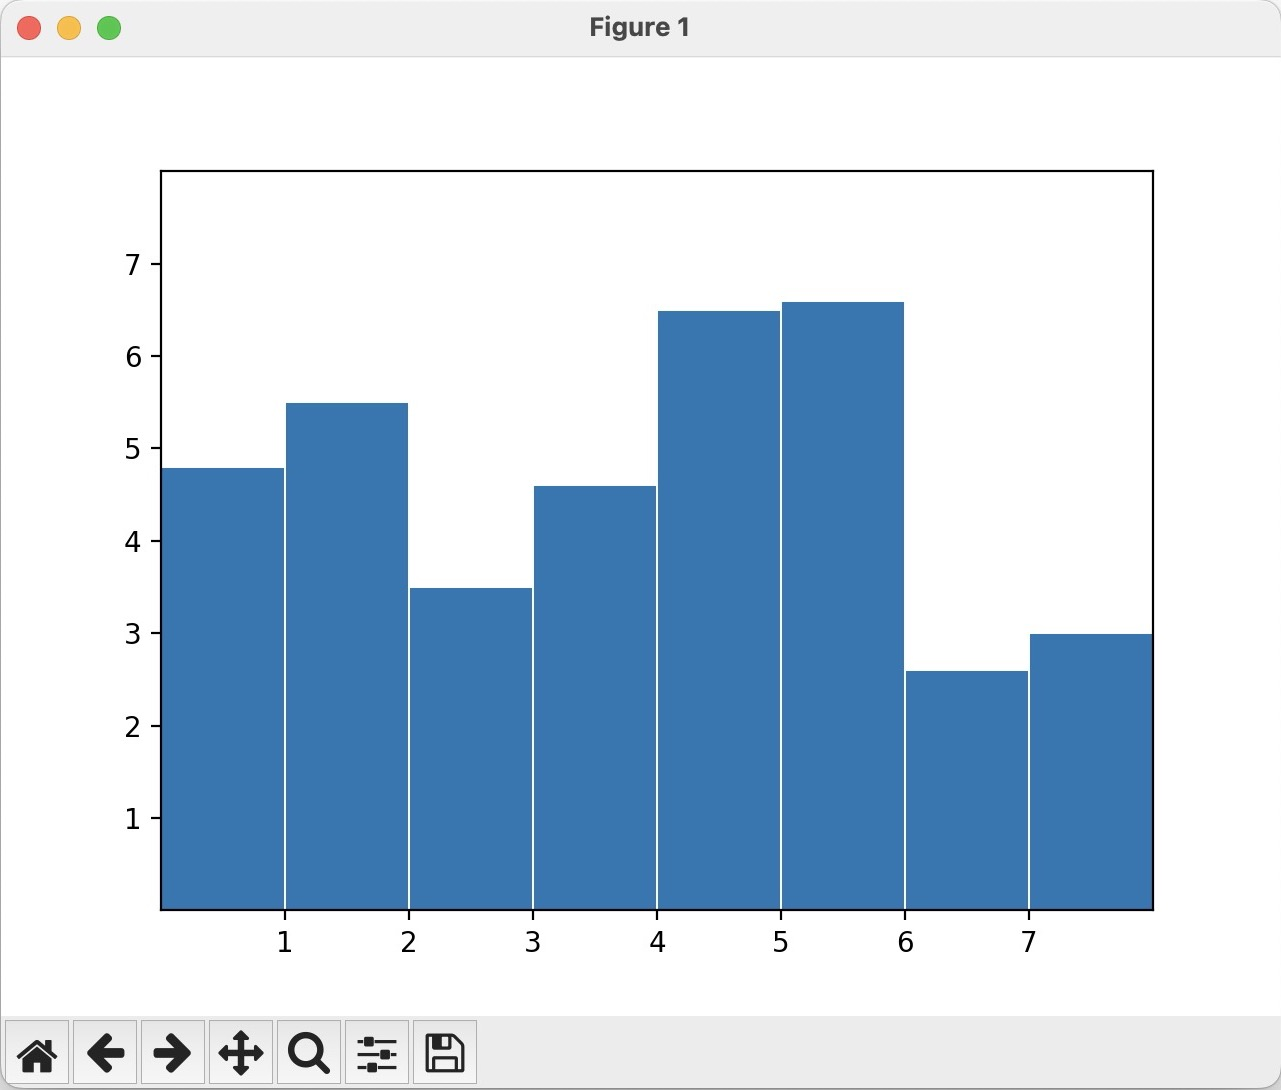
\includegraphics[width=.5\textwidth, trim={2.4mm 2mm 2mm 2mm},clip]{images/ch01/bar.jpg}};
    \drawshadow{image}
\end{tikzpicture}
\caption{} 
\label{fig:}
\end{figure}

လိုက်ဘရီတွေဟာ ပရိုဂရမ်တွေ တည်ဆောက်ရာမှာ အင်မတန်မှ အရေးပါတယ်။ ဖော်ပြထားတဲ့ မေ့ထရစ် နဲ့ ဘားချတ်  ကုဒ်တွေကို (အခုတော့) နားလည်မှာ မဟုတ်သေးဘူးပေါ့။ ဒါပေမဲ့ သက်ဆိုင်ရာ လိုက်ဘရီတွေနဲ့ ဒီလိုကိစ္စတွေကို သိပ်မခက်ခဲဘဲ လုပ်လို့ရနိုင်တယ်ဆိုတာ မြင်မယ် ထင်ပါတယ်။ လိုက်ဘရီတွေသာမရှိရင် ပရိုဂရမ်တွေကို အခုထက် အဆပေါင်းများစွာ အချိန်ပေးပြီး ရှုပ်ရှုပ်ထွေးထွေး ခက်ခက်ခဲခဲ တည်ဆောက်ကြရမှာပါ။ 


\subsection*{တုံကင်၊ စတိတ်မန့်နှင့် ဆင်းတက်စ်}
ဂျန်ပန်စာ၊ ပြင်သစ်စာ စတဲ့ လူ့ဘာသာစကားတွေဟာ  စကားလုံးတွေ ဝါကျတွေနဲ့ ဖွဲ့စည်းထားသလို ပရိုဂရမ်ကုဒ်တွေဟာလည်း စကားလုံးတွေ၊ ဝါကျတွေနဲ့ ဖွဲ့စည်းထားတာပါပဲ။ \fEn{Programming language} တွေမှာ စကားလုံးတွေကို တုံကင် \fEn{(\fEnEmpBf{token})} လို့ခေါ်ပြီး  ဝါကျတွေကိုတော့ စတိတ်မန့် \fEn{(\fEnEmpBf{statement})} လို့ ခေါ်ပါတယ်။ ဝါကျတွေကို စကားလုံးတွေနဲ့ ဖွဲ့စည်းထားသလို စတိတ်မန့်တွေကတော့ တုံကင်တွေနဲ့ ဖွဲ့စည်းထားတာပါ။ စတိတ်မန့် ပုံစံတစ်မျိုးကို တွေခဲ့ပြီးပါပြီ။ အဲဒါကတော့ ရှေ့စာမျက်နှာက အင်ပို့စတိတ်မန့်ပဲ ဖြစ်ပါတယ်။ 

လူ့ဘာသာစကားတွေမှာ ဖွဲ့စည်းတည်ဆောက်ပုံ စထရက်ချာရှိသလို \fEn{programming language} တွေမှာလည်း စထရက်ချာရှိဖို့ လိုအပ်တာပေါ့။  ဖွဲ့စည်းပုံ စထရက်ချာ မှန်/မမှန်ကို သဒ္ဒါစည်းမျဉ်တွေနဲ့ ထိန်းကွပ်ထားတာပါ။ ပရိုဂရမ်ကုဒ် စထရက်ချာ မှန်/မမှန် ထိန်းကွပ်ပေးတဲ့ သဒ္ဒါစည်းမျဉ်တွေကိုတော့ ဆင်းတက်စ် \fEn{(\fEnEmpBf{syntax})} လို့ခေါ်တယ်။

မြန်မာလိုရေးရင် မြန်မာသဒ္ဒါကို လိုက်နာရသလို \fEn{Python} နဲ့ ရေးရင် \fEn{Python} ဆင်းတက်စ်ကို လိုက်နာရမှာပေါ့။ မြန်မာသဒ္ဒါမှားရင် ဖတ်တဲ့သူက သည်းခံနားလည် ပေးပေမဲ့ ဆင်းတက်စ်မှားရင်တော့ \fEn{Python} က လုံးဝ လက်ခံမှာ မဟုတ်ပါဘူး။ ဆင်းတက်စ် စည်းကမ်းတွေဟာ ပိုပြီး တင်းကျပ်တယ်။ လွဲချော်လို့ မရဘူး။ ဆင်းတက်စ်မှားနေတဲ့ ပရိုဂရမ်ကို  \fEn{Python} က \fEn{run} ခွင့် ပြုမှာမဟုတ်ဘဲ အမှားနဲ့သက်ဆိုင်တဲ့ အယ်ရာ\fOpn{မက်ဆေ့ချ်}တွေ ပြပေးမှာပါ။ ဖြစ်လေ့ရှိတဲ့ ဆင်းတက်စ်အမှားတွေကို မကြာခင် တွေ့ရပါမယ်။

\subsection*{Keywords}
\fCode{from}\fEn{,} \fCode{import}\fEn{,} \fCode{def} \fEn{,} \fCode{if} စတာတွေဟာ \fEnEmpBf{keyword} တွေဖြစ်တယ်။ \fEn{Python} ရေးတဲ့အခါ သူ့နေရာနဲ့သူ အဓိပ္ပါယ်ကိုယ်စီနဲ့ အသုံးပြုရတဲ့ စကားလုံးတွေဖြစ်တယ်။ \fCode{from} နဲ့ \fCode{import} ကို လိုက်ဘရီ အင်ပို့လုပ်ဖို့ သုံးတယ်။ \fCode{def} ကို ဖန်ရှင် သတ်မှတ်တဲ့အခါ သုံးတယ်။ \fEn{Python} က သတ်မှတ်ထားတဲ့ နေရာတွေကလွဲလို့ အခြားကိစ္စတွေအတွက် \fEn{keyword} တွေကို အသုံးပြုလို့ မရပါဘူး။ ဒါကြောင့်  \fEn{keyword} တွေကို \fEn{reserved word} လို့လည်း ခေါ်တယ်။ 

\subsection*{\fSubSecCodeBf{main} ဖန်ရှင်}
\fEn{‘Meet Karel’} ပရိုဂရမ် အင်ပို့စတိတ်မန့် အပြီးမှာ တွေ့ရတာကတော့ \fCode{main} ဖန်ရှင်သတ်မှတ်ချက်ပါ။ ကြည့်ရအဆင်ပြေအောင် သူ့ချည်းသီးသန့် တစ်ဖြတ် ပြန်ပြပေးထားပါတယ်။
%
\setlength{\fboxsep}{0pt}
\begin{minted}[frame=\mintframe, framerule=\mintrule,framesep= \mintsep, xleftmargin=\xlftmargin
    , bgcolor=mintbgcolor,rulecolor=mintrulecolor
    , python3=true,escapeinside=ßß]{python}
def main():
    """Karel code goes here!"""
    move()
    move()
    move()
    pick_beeper()
    turn_left()
    move()
    move()

    turn_left()
    turn_left()
    turn_left()

    move()
    put_beeper()
# End of main
\end{minted}

\begin{mytcbox}
ဖန်ရှင် \fEn{(\fEnEmpBf{function})} ဆိုတာ ကိစ္စတစ်ခု လုပ်ဆောင်ပေးဖို့အတွက် ယူနစ်တစ်ခုအနေနဲ့ ဖွဲ့စည်းထားတဲ့ ပရိုဂရမ်ကုဒ် အစုအဝေးတစ်ခုပါပဲ။ ဖန်ရှင်ကို အသုံးပြုတဲ့အခါ ၎င်းရဲ့ လုပ်ငန်းတာဝန်အတိုင်း ဖန်ရှင်က လုပ်ဆောင်ပေးမှာ ဖြစ်တယ်။ ဖန်ရှင်အသုံးပြုတာကို ‘ဖန်ရှင်ကောလ်’  \fEn{(\textit{function call})} လုပ်တာလို့ ပြောတယ်။
\end{mytcbox}
%
\fCode{main} ဖန်ရှင်သတ်မှတ်ချက်ကို အပိုင်းနှစ်ပိုင်းခွဲ ကြည့်နိုင်တယ်။ ပထမတစ်ပိုင်း
%
\setlength{\fboxsep}{0pt}
\begin{minted}[frame=\mintframe, framerule=\mintrule,framesep= \mintsep, xleftmargin=\xlftmargin
    , bgcolor=mintbgcolor,rulecolor=mintrulecolor
    , python3=true,escapeinside=ßß]{python}
def main():
\end{minted}
%
ကို ဖန်ရှင်ခေါင်းစီး \fEn{(function header)} လို့ခေါ်တယ်။ ဖန်ရှင်ခေါင်းစီးမှာ ဖန်ရှင်နံမည်နဲ့ ဖန်ရှင်ပါရာမီတာတွေကို ဝိုက်ကွင်းထဲမှာ သတ်မှတ်ပေးရပြီး ကော်လံ \mytcboxinl{\fCode{:}} နဲ့ အဆုံးသတ်တယ်။ ဥပမာ \fCode{x}\fEn{,} \fCode{y} ပါရာမီတာ နဲ့  \fCode{myfun} ဖန်ရှင် အတွက် 
%
\setlength{\fboxsep}{0pt}
\begin{minted}[frame=\mintframe, framerule=\mintrule,framesep= \mintsep, xleftmargin=\xlftmargin
    , bgcolor=mintbgcolor,rulecolor=mintrulecolor
    , python3=true,escapeinside=ßß]{python}
def myfun(x, y):
\end{minted}
ပါရာမီတာမပါရင်လည်း ဝိုက်ကွင်းအလွတ် တစ်စုံ \mytcboxinl{\fCode{()}} တော့ပါရမယ်။ \fCode{main} ဖန်ရှင်မှာ ပါရာမီတာ မပါဘူး။ ပါရာမီတာတွေအကြောင်း နောက်ပိုင်းအခန်းတွေမှာ အသေးစိတ် လေ့လာရမှာပါ။ ကားရဲလ်ပရိုဂရမ်တွေမှာ ပါရာမီတာအကြောင်း သိဖို့မလိုသေးပါဘူး။ ပါရာမီတာ မလိုတဲ့ ဖန်ရှင်တွေပဲ တွေ့ရမှာပါ။ 

ဖန်ရှင်သတ်မှတ်ချက် ဒုတိယပိုင်းကတော့ ဖန်ရှင်ဘော်ဒီပါ။ ဖန်ရှင်ဘော်ဒီ ရေးရင် ဘေးမျဉ်းကနေ ညာဘက်ကို ခွာရေးရပါမယ်။ ခွာတဲ့ အကွာအဝေး တပြေးညီ ဖြစ်ရမယ်။  အင်ဒန့်ထ် \fEn{(indent)} လုပ်တာလို့ ခေါ်တယ်။ ကုဒ်စထရက်ချာကို ကြည့်လိုက်တာနဲ့ ထင်းကနဲ မြင်သာအောင် လုပ်ရတာပါ။ \fCode{main} ဖန်ရှင်မှာ ခေါင်းစီးအောက် အင်ဒန့်ထ်လုပ်ထားတဲ့ ကုဒ်အားလုံးဟာ ဖန်ရှင်ဘော်ဒီပဲလို့ ချက်ချင်းသိနိုင်တယ်။ ဘော်ဒီ ပထမတစ်ကြောင်း
%ချိန်ညှိရေးထားတဲ့
\setlength{\fboxsep}{0pt}
\begin{minted}[frame=\mintframe, framerule=\mintrule,framesep= \mintsep, xleftmargin=\xlftmargin
    , bgcolor=mintbgcolor,rulecolor=mintrulecolor
    , python3=true,escapeinside=ßß]{python}
"""Karel code goes here!"""
\end{minted}
ဟာ \fEnEmp{docstring} လို့ ခေါ်တဲ့ စာသား ဖြစ်တယ်။ ဖန်ရှင်နဲ့ ပါတ်သက်တဲ့ ရှင်းလင်းဖော်ပြချက်တွေ ရေးဖို့အတွက် သုံးတာပါ။ ဒါကြောင့် \fEn{docstring} ကို \fEn{quote} သုံးခုတွဲ \mytcboxinl{\fCode{"""}} တစ်စုံကြား ညှပ်ရေးတဲ့ ကွန်းမန့်တစ်မျိုးလို့ ယူဆနိုင်တယ်။ လိုအပ်တဲ့အခါ အသေးစိတ် ထပ်ပြီး ဖော်ပြပေးမှာပါ။

\fEn{Docstring} အောက်မှာ တွေ့ရတာကတော့ ကားရဲလ်ကွန်မန်းတွေဆိုတာ သိပါလိမ့်မယ်။ ကားရဲလ်ကွန်းမန်းတွေဟာ \fCode{stanfordkarel} လိုက်ဘရီ ဖန်ရှင်တွေပါ။ တနည်းအားဖြင့် \fCode{stanfordkarel} လိုက်ဘရီမှာ ကားရဲလ်ကွန်းမန်းတွေအတွက် ဖန်ရှင်သတ်မှတ်ချက်တွေ ပါဝင်တယ်။ ဖန်ရှင်တစ်ခုကို အသုံးပြုဖို့အတွက် အဲဒီဖန်ရှင်ကို ခေါ်ရပါတယ်။ ဒါကို  \fEnEmp{function call} ‘ဖန်ရှင်ကောလ်’ လုပ်တယ်လို့ ပြောတယ်။ ကားရဲလ်ကို ဘယ်ဘက်လှည့်စေချင်ရင် \fCode{turn\_left} ဖန်ရှင်ကောလ် လုပ်ရပါမယ်။ ဘိပါကောက်ခိုင်းချင်ရင် \fCode{pick\_beeper} ဖန်ရှင်ကောလ် လုပ်ရပါမယ်။ ဖန်ရှင်ကောလ် လုပ်တဲ့ ပုံစံက
%
\setlength{\fboxsep}{0pt}
\begin{minted}[frame=\mintframe, framerule=\mintrule,framesep= \mintsep, xleftmargin=\xlftmargin
    , bgcolor=mintbgcolor,rulecolor=mintrulecolor
    , python3=true,escapeinside=ßß]{python}
turn_left()
pick_beeper()
\end{minted}
စသည်ဖြင့် ဖြစ်တယ်။

\begin{mytcbox}
\fEn{Python} မှာ အင်ဒန့်ထ်ကို ဖြစ်ကတတ်ဆန်း လုပ်လို့မရဘူး။ ဘေးမျဉ်းကနေ ခွာတဲ့ အကွာအဝေး မညီတာနဲ့ ဆင်းတက်စ်အမှား ဖြစ်တယ်။ မလိုတဲ့နေရာမှာလည်း ခွာရေးလို့ မရဘူး။ ခေါင်းစီးကို ဘေးမျဉ်းနဲ့ ခွာထားကြည့်ပါ။ အယ်ရာဖြစ်တာကို တွေ့ရမယ်။ အင်ပို့စတိတ်မန့်လည်း ဘေးမျဉ်းနဲ့ ကွာနေလို့မရဘူး။ အခြား \fEn{language} တွေမှားလည်း အင်ဒန့်ထ်လုပ် ရေးကြပေမဲ့ \fEn{Python} မှာလောက် မတင်းကျပ်ဘူး။ အင်ဒန့်ထ်မလုပ်လည်း ဆင်းတက်စ်မှားတာ မဖြစ်ဘူး။
\end{mytcbox}

ကားရဲလ်ပရိုဂရမ်တစ်ခုမှာ \fCode{main} ဟာ  အထူးတာဝန်တစ်ခု လုပ်ဆောင်ပေးရတယ်။ အဲဒါကတော့ ပရိုဂရမ်ဝင်းဒိုးမှာ \mytcboxinl{\fEnSnd{Run Program}}  ခလုတ် (ပုံ \fRefNo{\ref{fig:mtkrlprgm1}} မှာကြည့်ပါ) နှိပ်လိုက်ရင် တုံ့ပြန် လုပ်ဆောင်ပေးရတာပါ။ ဒါကြောင့် ကွန်မန်းတွေဟာ အဲဒီခလုတ် နှိပ်တော့မှပဲ စအလုပ်လုပ်တာ ဖြစ်တယ်။

\subsection*{Entry Point (ပရိုဂရမ်စမှတ်)}
\fEn{‘Meet Karel’} ပရိုဂရမ်မှာ \fCode{main} ဖန်ရှင်နောက် အောက်ဆုံးအပိုင်းဟာ ပရိုဂရမ် \fEn{run} တဲ့အခါ ပထမဆုံး စတင်လုပ်ဆောင်ပေးရမဲ့ ဖန်ရှင်ကို ဖော်ပြပေးတာပါ။ ‘အန်ထရီပွိုင့်’ လို့ခေါ်တယ်။ 
%
\setlength{\fboxsep}{0pt}
\begin{minted}[frame=\mintframe, framerule=\mintrule,framesep= \mintsep, xleftmargin=\xlftmargin
    , bgcolor=mintbgcolor,rulecolor=mintrulecolor
    , python3=true,escapeinside=ßß]{python}
if __name__ == "__main__":
    run_karel_program("meet_karel")
\end{minted}
%
\fCode{run\_karel\_program} ဖန်ရှင်ဟာ ကားရဲပရိုဂရမ် တစ်ခုအတွက် အန်ထရီပွိုင့် ဖြစ်တယ်။  ပရိုဂရမ် တက်လာတာနဲ့ တစ်ပါတည်း ခေါ်တင်ချင်တဲ့ ကမ္ဘာကို ဒီဖန်ရှင်မှာ ထည့်ပေးတယ်။ \mytcboxinl{\fEnSnd{meet\_karel.w}} ကမ္ဘာကို စစချင်းခေါ်တင်ထားချင်ရင် \fCode{"meet\_karel"} ထည့်ပေးရမယ်။  ဖိုင်မရှိတဲ့ကမ္ဘာကို ထည့်ထားရင် အယ်ရာတက်ပြီး ပရိုဂရမ်ပွင့်လာမှာ မဟုတ်ဘူး။ ကမ္ဘာမထည့်ပေးထားဘဲ ဒီလို
%
\setlength{\fboxsep}{0pt}
\begin{minted}[frame=\mintframe, framerule=\mintrule,framesep= \mintsep, xleftmargin=\xlftmargin
    , bgcolor=mintbgcolor,rulecolor=mintrulecolor
    , python3=true,escapeinside=ßß]{python}
run_karel_program()
\end{minted}
%
ဆိုရင် $8 \times 8$ အရွယ် \fEn{default} ကမ္ဘာကို တင်ပေးပါတယ်။

ကားရဲလ်ကမ္ဘာတစ်ခုကို လိုချင်တဲ့ပုံစံ ဒီဇိုင်းဆွဲပြီး ဖိုင်နဲ့ သိမ်းထားရတာပါ။ ကမ္ဘာ ပုံစံချတဲ့ ပရိုဂရမ်လည်း ရှိတယ်။ ကမ္ဘာဖိုင်တွေက \mytcboxinl{\fEnSnd{.w}} ဖိုင် အိပ်စ်တန်းရှင်းနဲ့ ဖြစ်တယ်။ ဒီစာအုပ်မှာပါတဲ့ ဥပမာတွေ၊ လေ့ကျင့်ခန်းတွေ အားလုံးအတွက် လိုအပ်တဲ့ ကမ္ဘာတွေကို အဆင်သင့်ပေးထားမှာပါ။ ကိုယ့်ဟာကို လုပ်ဖို့ မလိုဘူး။ စိတ်ဝင်စားရင် စမ်းကြည့်လို့ရအောင် စာမျက်နှာ (\fRefNo{\pageref{apdx:02}}) နောက်ဆက်တွဲ (\fRefNo{\ref{apdx:02}}) မှာ အကျဉ်းဖော်ပြပေးထားပါတယ်။

\section{ကားရဲလ် ပရိုဂရမ် run ခြင်း}

လိုအပ်တဲ့ဆော့ဖ်ဝဲတွေ ထည့်သွင်းနည်းကို စာမျက်နှာ (\fRefNo{\pageref{apdx:01}}) နောက်ဆက်တွဲ (\fRefNo{\ref{apdx:01}}) မှာ တစ်ဆင့်ချင်း ဖော်ပြပေးထားပါတယ်။ အခုက \fEn{Python} ပရိုဂရမ်တစ်ခုကို အရိုးရှင်းဆုံး (လွယ်တယ်လို့ မဆိုလို)  \fEn{run} လို့ရတဲ့ နည်းကိုဖော်ပြပေးမှာပါ။ သဘောတရားပိုင်း နားလည်ဖို့ အထောက်အပံ့ဖြစ်မယ်။ အခုနည်းလမ်းကို အကြမ်းဖျဉ်း နားလည်အောင် ဖတ်ပြီးမှ နောက်ဆက်တွဲ (\fRefNo{\ref{apdx:01}}) ကို ဖတ်စေချင်ပါတယ်။

မိုက်ခရိုဆော့ဖ် ဝင်းဒိုးမှာ \fEn{Notepad} ၊ အက်ပဲလ် မက်ခ်အိုအက်စ်မှာ  \fEn{TextEdit} စတဲ့ တက်စ် အယ်ဒီတာတစ်ခုခုနဲ့ ပရိုဂရမ်ကုဒ်ရေးလို့ရတယ်။ ကုဒ်ဖိုင်ကို \mytcboxinl{\fEnSnd{.py}} အိပ်စ်တန်းရှင်းနဲ့ သိမ်းရပါမယ်။ ပလိန်းတက်စ် \fEn{(plain text)} ဖိုင် ပါပဲ။ \fEn{Python} ကုဒ်ဖိုင်မို့လို့ \mytcboxinl{\fEnSnd{.txt}} အစား \mytcboxinl{\fEnSnd{.py}} နဲ့ သိမ်းတာပါ။ \fEn{Python} ဖိုင် နံမည်ကို စာလုံးအသေးနဲ့ပဲ ပေးတဲ့ ထုံးစံရှိတယ်။  စပေ့စ်နေရာမှာ \mytcboxinl{\fEnSnd{ \_}} \fEn{(underscore)} သုံးတဲ့ ထုံးစံရှိတယ်။ ဒါကြောင့် \fEn{‘Meet Karel’} ပရိုဂရမ်ကုဒ်ကို \mytcboxinl{\fEnSnd{meet\_karel.py}} ဖိုင်မှာ သိမ်းသင့်တယ်။ 

\fEn{Python} နဲ့ ရေးထားတဲ့ ပရိုဂရမ်ကို \fEn{run} မယ်ဆိုရင် \fEn{Python} ဆော့ဖ်ဝဲရှိရမှာပါ။ ဒီဆော့ဖ်ဝဲ အင်စတောလ် လုပ်နည်းကို နောက်ဆက်တွဲ (\fRefNo{\ref{apdx:01}}) စာမျက်နှာ (\fRefNo{\pageref{subsec:pyinstl}}) မှာ ဖော်ပြပေးထားပါတယ်။ \fEn{Python} ကုဒ်တွေကို ကွန်ပျူတာက တိုက်ရိုက် နားမလည်ပါဘူး။ \fEn{Python} ဆော့ဖ်ဝဲဟာ \fEn{Python} ကုဒ်တွေကို တိုက်ရိုက် နားလည်ပြီး ကွန်ပျူတာပေါ်မှာ \fEn{run} လို့ရအောင် ကြားခံဆောင်ရွက်ပေးတဲ့ ဆော့ဖ်ဝဲလို့ ယေဘုယျအားဖြင့် ယူဆနိုင်တယ်။

\fEn{Python} ထည့်ပြီးရင် \fCode{stanfordkarel} လိုက်ဘရီကို အောက်ပါကွန်မန်းနဲ့ အင်စတောလ် လုပ်ရပါမယ်။ အင်တာနက်ပေါ်ကနေ ဒေါင်းလုဒ် လုပ်ရတာမို့လို့ ကွန်နက်ရှင်ရှိရမယ်။
%
\begin{minted}[frame=lines, framerule=0pt]{text}
pip install stanfordkarel
\end{minted}
%

ကားရဲလ်ပရိုဂရမ်မှာ ခေါ်တင်ချင်တဲ့ ကမ္ဘာဖိုင်တွေလည်း ရှိရပါမယ်။  \fEnSnd{meet\_karel.w} ကမ္ဘာဖိုင်က \fEnSnd{meet\_karel.zip} ဖိုင် \fEnSnd{worlds} ဖိုဒါထဲမှာ ရှိပါတယ်။  \fCode{http://tinyurl.com/3mmm9c7j} လင့်ကနေ \fEnSnd{meet\_karel.zip}  ဖိုင်ကို ဒေါင်းလုဒ်လုပ်ပါ။ ဒီ \fEnSnd{zip} ဖိုင်ထဲက \fEnSnd{worlds} ဖိုဒါကို \mytcboxinl{\fEnSnd{meet\_karel.py}} ဖိုင်ရှိတဲ့နေရာမှာ ကော်ပီကူးထည့်ပါ။ ဝင်းဒိုးမှာ \fEn{Command Prompt} ၊ မက်ခ်အိုအက်စ်မှာ  \fEn{Terminal} ဖွင့်ပြီး \mytcboxinl{\fEnSnd{cd}} ကွန်မန်းနဲ့ ကုဒ်ဖိုင်ထားတဲ့ ဖိုဒါထဲကို သွားပြီး အောက်ပါအတိုင်း \mytcboxinl{\fEnSnd{python}} ကွန်မန်းနဲ့ ကုဒ်ဖိုင်ကို \fEn{run} ပေးရပါမယ် (လာမဲ့စာမျက်နှာမှာ နမူနာပြထားတာ ကြည့်ပါ)။ 
%
\begin{minted}[frame=lines, framerule=0pt,escapeinside=ßß]{text}
python meet_karel.py
\end{minted}
ကုဒ်ရေးထားတာ ဆင်းတက်စ်အမှား မရှိဘူးဆိုရင် ကားရဲပရိုဂရမ် ပွင့်လာမှာပါ။

အခုဖော်ပြခဲ့တာက ကားရဲလ်ပရိုဂရမ်တစ်ခု \fEn{run} ဖို့ မဖြစ်မနေလုပ်ရမဲ့ အနည်းဆုံးလိုအပ်ချက်ပါ။ \fEn{Python} ဆော့ဖ်ဝဲ ရှိရမယ်။ \fCode{stanfordkarel} လိုက်ဘရီ အင်စတောလ် လုပ်ရမယ်။ ကမ္ဘာဖိုင်ပါတဲ့ \fEnSnd{worlds} ဖိုဒါရှိရမယ်။ \mytcboxinl{\fEnSnd{.py}} ဖိုင် တစ်ခုနဲ့ ပရိုဂရမ်ကုဒ်ကို သိမ်းရမယ်။ \fEnSnd{worlds} ဖိုဒါနဲ့ ကုဒ်ဖိုင်ကို တစ်နေရာတည်းမှာ ထားရမယ်။ ပြီးရင် ကွန်မန်းလိုင်းမှာ 
%
\begin{minted}[frame=lines, framerule=0pt,escapeinside=ßß]{text}
python your_karel_program.py
\end{minted}
\fEn{run} ရုံပါပဲ။

\mytcboxinl{\fEnSnd{C:{\textbackslash}Users{\textbackslash}pyiso{\textbackslash}FirstKarelProgram}} ဖိုဒါထဲမှာ ကုဒ်ဖိုင်နဲ့ \fEnSnd{worlds} ဖိုဒါကို ထားပြီး ဘယ်လို \fEn{run} ရလဲ နမူနာပြထားတာကို ကြည့်ပါ။
\begin{figure}[tbh!]
\begin{tikzpicture}
    \node[anchor=south west,inner sep=0] (image) at (0,0)
        {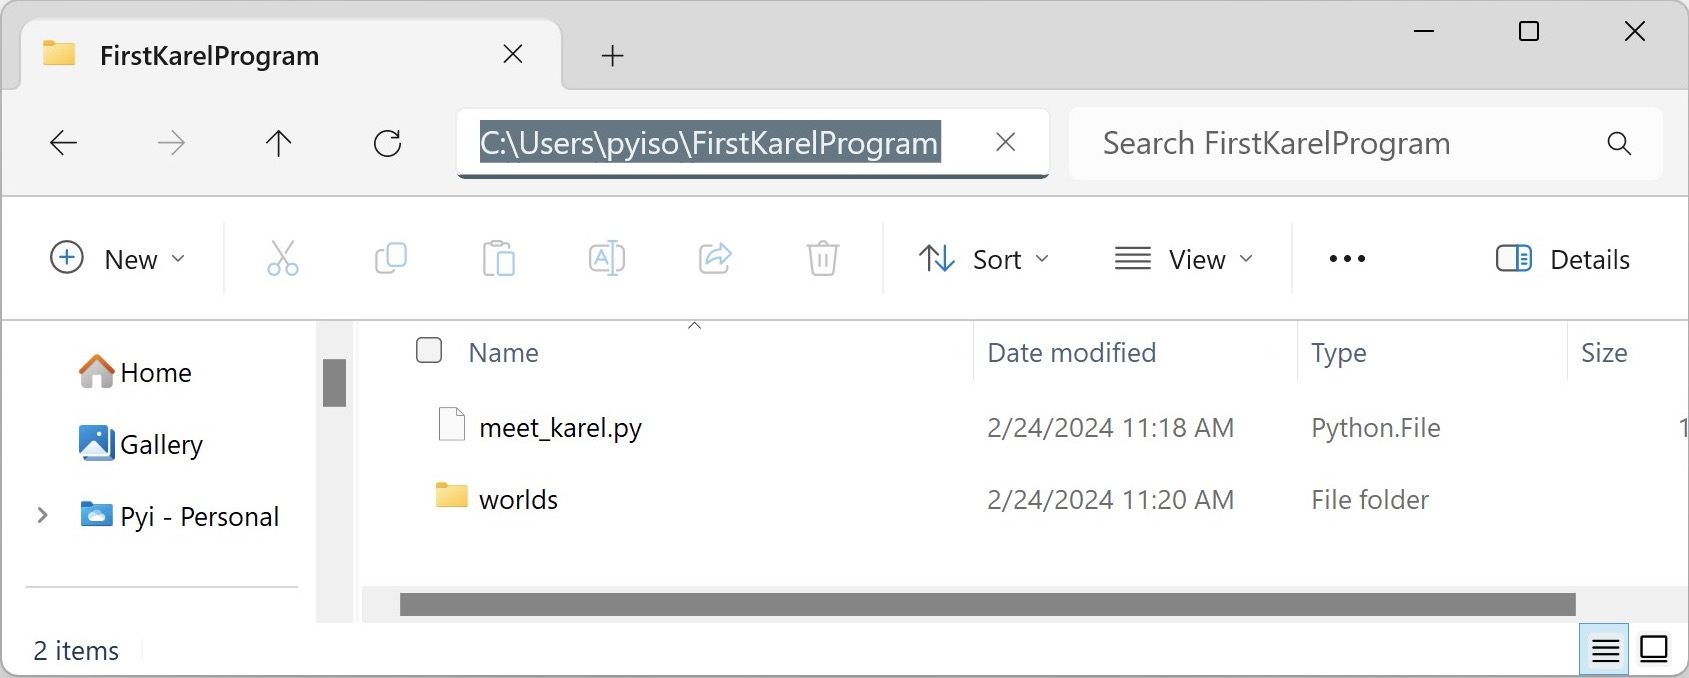
\includegraphics[width=.98\textwidth, trim={2.4mm 2mm 2mm 2mm},clip]{images/ch01/projstruct.jpg}};
    \drawshadow{image}
\end{tikzpicture}
\caption{} 
\label{fig:projstruct}
\end{figure}

\begin{figure}[tbh!]
\begin{tikzpicture}
    \node[anchor=south west,inner sep=0] (image) at (0,0)
        {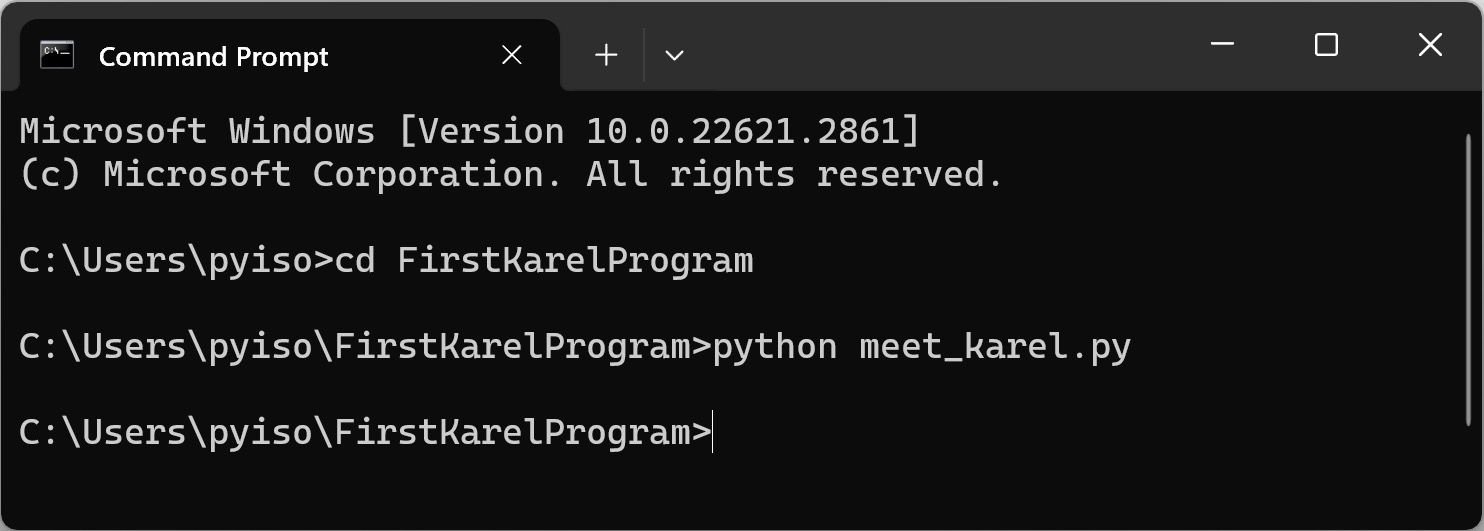
\includegraphics[width=.98\textwidth, trim={2.4mm 2mm 2mm 2mm},clip]{images/ch01/runkrl.jpg}};
    \drawshadow{image}
    \draw [draw=red, thick,rounded corners] (2.825,2.58) rectangle (6.65,2);
    \draw [draw=red, thick,rounded corners] (6.1,1.83) rectangle (10,1.25);

\end{tikzpicture}
\caption{} 
\label{fig:runkrl}
\end{figure}

\begin{figure}[tbh!]
\begin{tikzpicture}
    \node[anchor=south west,inner sep=0] (image) at (0,0)
        {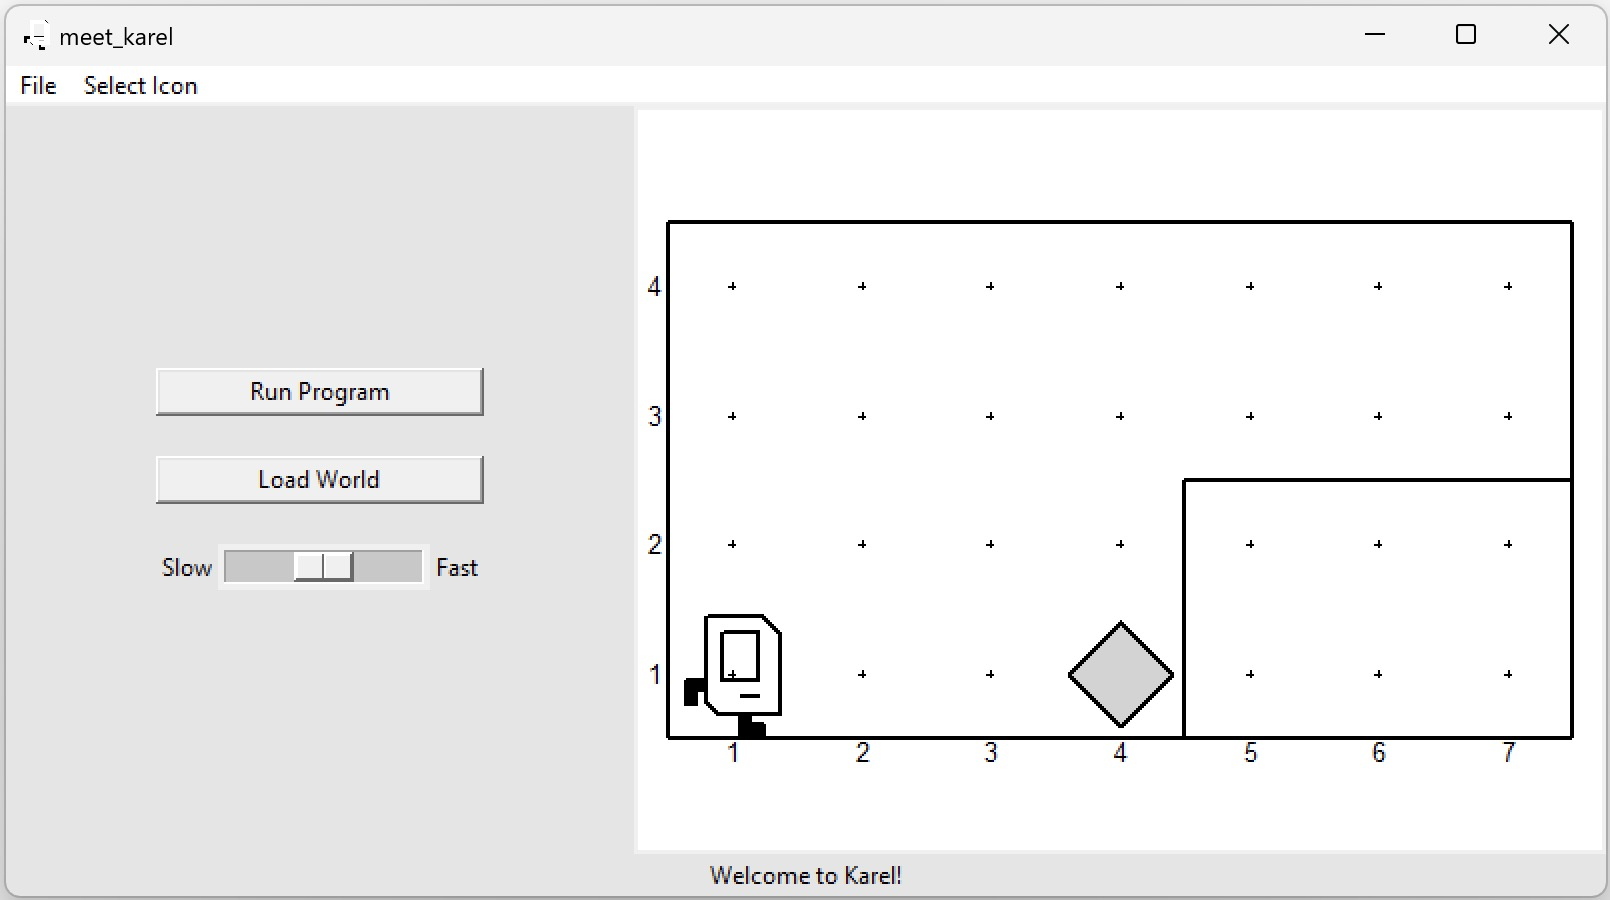
\includegraphics[width=.98\textwidth, trim={2.4mm 2mm 2mm 2mm},clip]{images/ch01/mtkrlprgm.jpg}};
    \drawshadow{image}
\end{tikzpicture}
\caption{} 
\label{fig:mtkrlprgm1}
\end{figure}

\section{Move Beeper to Other Side}
ပရိုဂရမ်းမင်း လေ့လာတဲ့အခါ စာချည်းပဲ ဖတ်နေပြီး အမှန်တကယ် နားလည်သွားဖို့ဆိုတာ မဖြစ်နိုင်ပါဘူး။ လက်တွေ့ စမ်းသပ်ကြည့်၊ ရေးကြည့်မှပဲ တကယ် နားလည်လာမယ်။ တကယ်လည်း ကျွမ်းကျွမ်းကျင်ကျင် ရေးတတ်လာမှာပါ။ ဒါကြောင့် လက်တွေ့ရေးကြည့်ပါ။ များများ လေ့ကျင့်ပါ။ ဥပမာတွေကိုလည်း နားလည်အောင် ဖတ်ပြီးရင် မိမိဘာသာ အလွတ် ပြန်ရေးကြည့်ပါ။ 

ပုံ (\fRefNo{\ref{fig:mbtos}}) မှ ဘိပါကို နံရံအခြားတစ်ဘက် အောက်ခြေကို ရွှေ့ပေးတဲ့ ပရိုဂရမ် ရေးကြည့်ပါ။ \fEn{Python} ထုံးစံအရ \mytcboxinl{\fEnSnd{move\_beeper\_to\_other\_side.py}} ဖိုင်နဲ့ သိမ်းသင့်ပါတယ်။ \mytcboxinl{\fEnSnd{meet\_karel.zip}} ဖိုင်ထဲမှာပါတဲ့ \fEnSnd{worlds} ဖိုဒါမှာပဲ အခု ကမ္ဘာဖိုင် ထည့်ပေးထားပါတယ်။ \mytcboxinl{\fEnSnd{move\_beeper\_to\_other\_side.w}} နံမည်နဲ့ပါ။ အန်ထရီပွိုင့်အတွက် အခုလိုရေးရပါမယ်။

\setlength{\fboxsep}{0pt}
\begin{minted}[frame=\mintframe, framerule=\mintrule,framesep= \mintsep, xleftmargin=\xlftmargin
    , bgcolor=mintbgcolor,rulecolor=mintrulecolor
    , python3=true,escapeinside=ßß]{python}
if __name__ == "__main__":
    run_karel_program("move_beeper_to_other_side")
\end{minted}

\begin{figure}[tbh!]
\begin{tikzpicture}
    \node[anchor=south west,inner sep=0] (image) at (0,0)
        {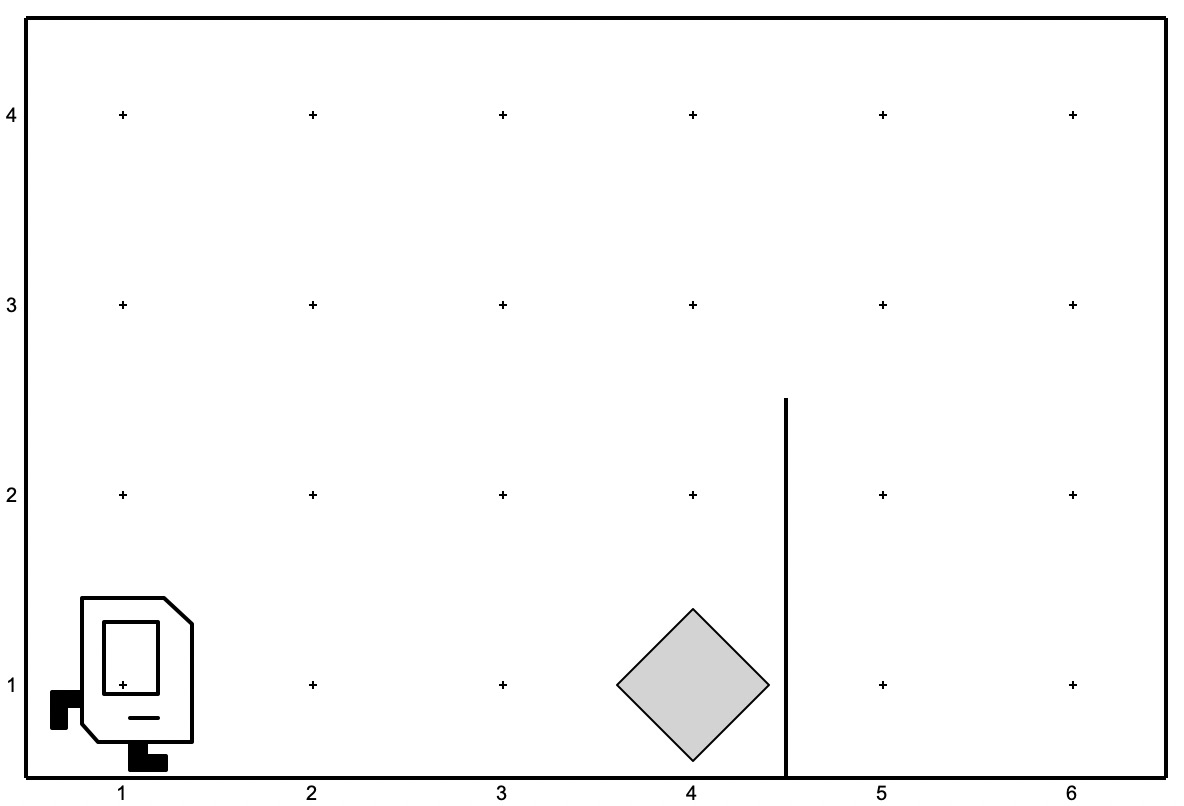
\includegraphics[width=3.5in, trim={2.4mm 2mm 2mm 2mm},clip]{images/ch01/MoveBeeperToOtherSide.jpg}};
    
\end{tikzpicture}
\caption{} 
\label{fig:mbtos}
\end{figure}


%

%

%
%
%
%အထက်ဖော်ပြပါ ပရိုဂရမ်ကုဒ် ပထမဆုံးတစ်ကြောင်းဟာ \fCode{import} စတိတ်မန့် ဖြစ်ပါတယ်။ ပရိုဂရမ်ကုဒ်ထဲမှာ ကလပ်စ် \fEn{(Class)} တစ်ခုကို ရည်ညွှန်းအသုံးပြုလို့ရအောင် \fCode{import} လုပ်ပေးရတာပါ။
%%
%\begin{minted}[frame=lines, framerule=0pt]{java}
%import stanford.karel.Karel;
%\end{minted}
%%
% \fCode{stanford.karel} \fOpn{ပက်ကေ့ချ်} \fEn{(package)} မှ \fCode{Karel} ကလပ်စ်ကို \fCode{import} လုပ်ထားတာ ဖြစ်တယ်။ စတိတ်မန့် အဆုံးမှာ ဆီမီးကော်လံ \fEn{(\fCode{;})} ပါတာကို သတိပြုပါ။ \fEn{Java} မှာ စတိတ်မန့် တစ်ကြောင်းဆုံးတိုင်း ဆီမီးကော်လံ ထည့်ပေးရပါမယ်။ \fOpn{ပက်ကေ့ချ်}ဆိုတာ ဆက်စပ်ရာ ကလပ်စ်တွေ စုစည်းထားတဲ့ ယူနစ်တစ်ခုပါပဲ။ \fCode{stanford.karel} \fOpn{ပက်ကေ့ချ်}ထဲက ကလပ်စ်အားလုံးကို \fCode{import} လုပ်မယ်ဆိုရင် ဒီလိုရေးရတယ်။
%%
%\begin{minted}[frame=lines, framerule=0pt]{java}
%import stanford.karel.*;
%\end{minted}
%%  
%လိုအပ်တဲ့ ကလပ်စ်ကိုပဲ ရွေးပြီး \fCode{import} လုပ်တာ ပိုကောင်းပါတယ်။
%
%\subsection*{ကလပ်စ်}
%ကလပ်စ် \fEn{(Class)} အကြောင်းကို နောက်ပိုင်းမှာ လေ့လာကြရမှာပါ။ အခုလောလောဆယ် ကလပ်စ်ကို ပရိုဂရမ်ကုဒ် စထရက်ချာတစ်မျိုးဟု ယူဆပါ။ \fEn{Java} ပရိုဂရမ်တစ်ခုမှာ အနည်းဆုံး ကလပ်စ်တစ်ခု ရှိရပါမယ်။ ကလပ်စ်တစ်ခုဖြစ်ဖို့အတွက် ဆင်းတက်စ်အရ အနည်းဆုံးရှိရမဲ့ ပုံစံက ဒီလိုပါ။
%%
%\begin{minted}[frame=lines, framerule=0pt]{java}
%public class MeetKarel {
%
%}
%\end{minted}
%% 
%ကလပ်စ်နံမည်က \fCode{MeetKarel} ဖြစ်ပါတယ်။ စကားလုံးအားလုံး အကြီးစာလုံးနဲ့ စထားတာ သတိထားကြည့်ပါ။ \fCode{meetkarel} လို့ရေးတာထက်  \fCode{MeetKarel} က စကားလုံးတစ်လုံးချင်းကို ပိုပြီးထင်ရှားစေတယ်။ ဒါကြောင့် အကြီးနဲ့စတဲ့ နည်းကိုပဲ အကြံပြုပါတယ်။
%
%\subsection*{\fSubSecCodeBf{Karel} ကလပ်စ်ကို \fSubSecCodeBf{extends} လုပ်ခြင်း}
%ရှေ့မှာတွေ့ခဲ့တဲ့ \fCode{MeetKarel} ကလပ်စ်ဟာ ကလပ်စ်အခွံချည်း ဖြစ်တယ်။ တွန့်ကွင်း အဖွင့်အပိတ်ကြားဟာ အလွတ်ဖြစ်နေပြီး ဘာပရိုဂရမ်ကုဒ်မှ မပါသေးပါဘူး။ ဒီကလပ်စ်ကို ကားရဲလ်ပရိုဂရမ်ဖြစ်အောင် အခုလိုရေးရပါမယ်။
%%
%\begin{minted}[frame=lines, framerule=0pt]{java}
%import stanford.karel.Karel;
%
%public class MeetKarel extends Karel {
%    
%}
%\end{minted}
%%
%\fCode{MeetKarel} ကလပ်စ်ဟာ \fCode{Karel} ကလပ်စ်ကို \fCode{extends} လုပ်ထားပါတယ်။ ပရိုဂရမ်ကုဒ်မှာ \fCode{Karel} ကလပ်စ်ကို ရည်ညွှန်းအသုံးပြုနိုင်ဖို့ အပေါ်မှာ \fCode{import} လုပ်ထားရတာပါ။ အခုအတိုင်းပဲ \fCode{MeetKarel}  ကို \fEn{IntelliJ} မှာ \fEn{run} ကြည့်ရင် ပုံ (\fRefNo{\ref{fig:meet_karel_window}}) မှာပြထားတဲ့ ကားရဲလ်ပရိုဂရမ် \fEn{window} တက်လာတာ တွေ့ရမှာပါ။ အဲဒီလိုမျိုး ကားရဲလ်ကမ္ဘာနဲ့ ဂရပ်ဖစ် \fEn{window} စခရင်ပေါ်မှာ ပေါ်လာတာဟာ  \fCode{Karel} ကလပ်စ်ထဲမှာ ပရိုဂရမ် ရေးပေးထားတဲ့ အတွက်ကြောင့် ဖြစ်တယ်။
%
%မှတ်ချက်။\qquad ။ အခုကစပြီး စာချည်းပဲဖတ်မနေဘဲ လက်တွေ့ပါ လိုက်လုပ်ကြည့်ဖို့ အလေးအနက် အကြံပြုချင်ပါတယ်။ စာမျက်နှာ \fRefNo{\pageref{apdx1}} နောက်ဆက်တွဲ (က) မှာ ဖော်ပြထားတဲ့အတိုင်း လိုအပ်တဲ့ ဆော့ဖ်ဝဲတွေထည့်သွင်းပါ။ နမူနာပါတဲ့ \fCode{MeetKarel} ပရိုဂရမ်ကို \fEn{run} ကြည့်ပါ။ 
%
%\begin{figure}[tb!]
%\begin{tikzpicture}
%    \node[anchor=south west,inner sep=0] (image) at (0,0)
%        {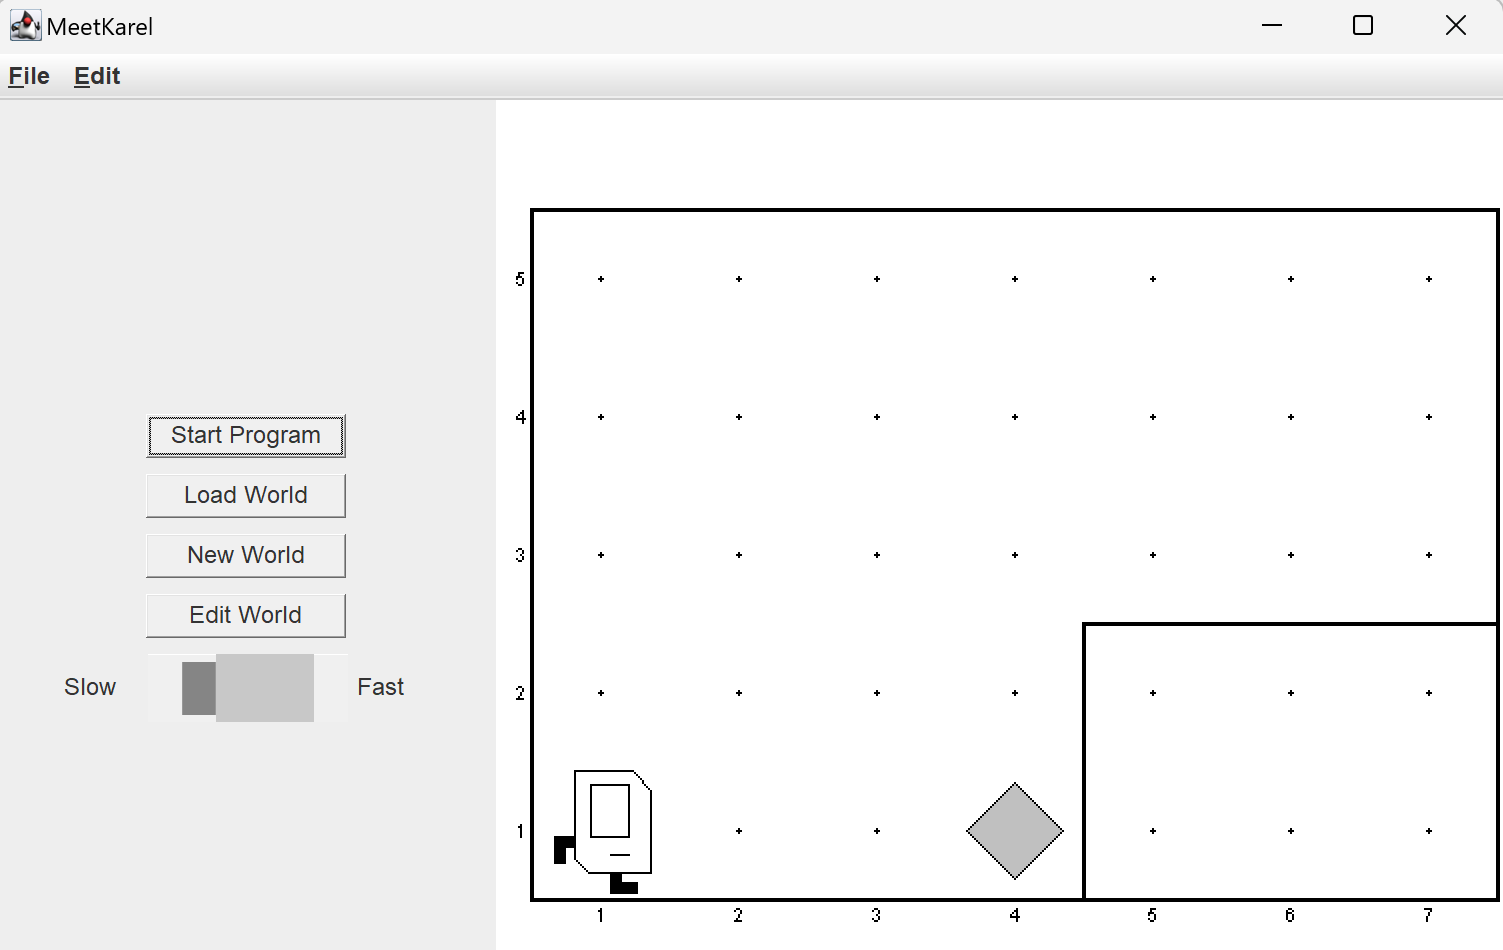
\includegraphics[width=.9\linewidth]{images/intellij_proj_create/MeetKarel.png}};
%    \drawshadow{image}
%\end{tikzpicture}
%\caption{}
%\label{fig:meet_karel_window}
%\end{figure}
%
%\subsection*{\fSubSecCodeBf{run} မက်သဒ်}
%
%မက်သဒ်ဆိုတာ စတိတ်မန့်တစ်စုကို ယူနစ်တစ်ခုအနေနဲ့ ဖွဲ့စည်းထားဖို့ အသုံးပြုတဲ့ စထရက်ချာတစ်မျိုးပါပဲ။ \fCode{move} စတိတ်မန့် သုံးခုကို ယူနစ်တစ်ခုအဖြစ် စုဖွဲ့ပေးထားတဲ့ \fCode{run} မက်သဒ်ကို အခုလိုတွေ့ရပါမယ်။ 
%%
%\begin{minted}[frame=lines, framerule=0pt]{java}
%import stanford.karel.Karel;
%
%public class MeetKarel extends Karel {
%    public void run() {
%        move();
%        move();
%        move();
%    }
%}
%\end{minted}
%%
%\fCode{run} မက်သဒ်ဟာ ကလပ်စ်ဘော်ဒီထဲမှာ ရှိရပါမယ်။ \fCode{run} ကို ဘယ်သူမဆို သုံးလို့ရအောင် \fCode{public} မက်သဒ်အနေနဲ့ သတ်မှတ်ထားတယ်။ \fCode{run} ဟာ \fCode{void} မက်သဒ်လည်းဖြစ်တယ်။ ဘာတန်ဖိုးမှ ပြန်ထုတ်မပေးတဲ့ မက်သဒ်လို့ အဓိပ္ပါယ်ရတယ်။  မက်သဒ်နံမည် \fCode{run} ဘေးမှာ ဝိုက်ကွင်းတစ်စုံပါရမယ်။ တွန့်ကွင်းတစ်စုံကတော့ မက်သဒ်ဘော်ဒီ အစနဲ့အဆုံးကို သတ်မှတ်ပေးထားတာ။ မက်သဒ်ဘော်ဒီထဲမှာ သက်ဆိုင်တဲ့ စတိတ်မန့်တွေ ရေးပေးရမယ်။ မက်သဒ်တွေအကြောင်း တစ်ခန်းသတ်သတ် လေ့လာကြရမှာပါ။ အဲဒီကျရင် အခုသိပ်နားမလည်တာတွေ အားလုံးရှင်းသွားပါလိမ့်မယ်။
%
%\fCode{run} ဟာ ကားရဲလ်ပရိုဂရမ်တွေအတွက် အထူးစီမံထားတဲ့ မက်သဒ်တစ်ခု ဖြစ်တယ်။ ပုံ (\fRefNo{\ref{fig:meet_karel_window}}) ကားရဲလ်ပရိုဂရမ် \fEn{window} ပေါ်လာပြီး \fEn{“Start Program”} နှိပ်လိုက်ရင် \fCode{run} မက်သဒ်ကို လုပ်ဆောင်ပေးတယ်။ \fEn{“Start Program”} မနှိပ်သေးရင် \fCode{run} နဲ့ဆိုင်တဲ့ စတိတ်မန့်တွေကလည်း အလုပ်မလုပ်သေးပါဘူး။ နှိပ်လိုက်တော့မှ \fCode{run} က စပြီးအလုပ်လုပ်တာပါ။ \fEn{“Start Program”} နှိပ်တဲ့အခါတိုင်း \fCode{run} ကို လုပ်ဆောင်ပေးမှာပါ။ 
%
%\fCode{MeetKarel} ကို အပေါ်မှာ ပြထားတဲ့အတိုင်း \fEn{IntelliJ} မှာ ရေးပြီး \fEn{run} ကြည့်ပါ။ \fEn{“Start Program”} နှိပ်လိုက်ရင် ကားရဲလ်က ရှေ့ကို သုံးခါရွှေ့ပေးပါလိမ့်မယ်။ နောက်ထပ်တစ်ခါ ထပ်နှိပ်ရင် \fCode{run} ကလည်း တစ်ခါထပ် အလုပ်လုပ်မှာပါ။ ဒါပေမဲ့ ရှေ့မှာ နံရံပိတ်နေတဲ့အတွက် ရွှေ့လို့မရတော့ဘဲ အယ်ရာတက်ပါလိမ့်မယ်။ \fEn{“Load World”} ကို နှိပ်ပြီး \fEn{MeetKarel.w} ဖိုင်ကိုရွေးလိုက်ရင် နဂိုအနေအထားပြန်ဖြစ်သွားပါလိမ့်မယ်။ ဒါမှမဟုတ် ပရိုဂရမ်ကို ပိတ်ပြီး ပြန် \fEn{run} နိုင်ပါတယ်။
%
%\subsection*{မက်သဒ်ကောလ် စတိတ်မန့်}
%\fCode{run} မက်သဒ်ထဲမှာတွေ့ရတဲ့ စတိတ်မန့်တွေဟာ မက်သဒ်ကောလ် \fEn{(method call)} စတိတ်မန့်တွေဖြစ်ပါတယ်။ \fCode{move}\fEn{,} \fCode{pickBeeper}\fEn{,}  \fCode{putBeeper}\fEn{,} \fCode{turnLeft} ကွန်မန်းတွေဟာ \fCode{Karel} ကလပ်စ်မှာ သတ်မှတ်ပေးထားတဲ့ မက်သဒ်တွေဖြစ်တယ်။ ပရိုဂရမ်ရေးတဲ့အခါ ကားရဲလ်ကွန်မန်းတွေကို မက်သဒ်ကောလ် စတိတ်မန့်အနေနဲ့ ရေးရမယ်။ ဥပမာ ဘယ်ဘက် လှည့်ခိုင်းတာကို
%%
%\begin{minted}[frame=lines, framerule=0pt]{java}
%turnLeft();
%\end{minted}
%%
%လို့ ရေးရပါမယ်။ စတိတ်မန့်ဖြစ်တဲ့အတွက် ဆီမီးကော်လံချပေးရမှာ ဂရုပြုပါ။ 
%
%\subsection*{မှတ်ချက်ရေးခြင်း}
%ဘိပါကို နေရာရွှေ့ထားဖို့ အပြီးထိဆက်ရေးထားတဲ့ ပရိုဂရမ်ကို အောက်မှာ ပြန်ဖော်ပြပေးထားပါတယ်။ မှတ်ချက် \fEn{(comment)} ရေးထားတာ တချို့ ပါနေတာကလွဲရင် စာမျက်နှာ \fRefNo{\pageref{lst:MeetKarel1}} မှာ ဖော်ပြခဲ့တဲ့ ပရိုဂရမ်နဲ့ တူတူပါပဲ။
%%
%\begin{minted}[frame=lines, framerule=0pt]{java}
%/* 
%This is our first example Karel program. This program is for 
%moving the beeper to(5,3) corner.
%*/
%import stanford.karel.Karel;
%
%public class MeetKarel extends Karel {
%    public void run() {
%        move();
%        move();
%        move();
%        pickBeeper();
%        turnLeft();
%        move();
%        move();
%        // we want karel to turn right
%        // turning left 3 times is the same as turning right
%        turnLeft();
%        turnLeft();
%        turnLeft();
%        move();
%        putBeeper();
%    }
%}
%\end{minted}
%% 
%ကွန်းမန့်ရေးချင်ရင် \fCode{/*} နဲ့ \fCode{*/} အတွင်း သို့မဟုတ် \fCode{//} နောက်မှာ ရေးရပါတယ်။ ကွန်းမန့်တွေကို ပရိုဂရမ်ကုဒ်အနေနဲ့ မယူဆရပါဘူး။ တနည်းအားဖြင့် ကွန်းမန့်တွေဟာ ကွန်ပျူတာ ဆောက်ရွက်ပေးရမဲ့ ညွှန်ကြားချက်တွေ မဟုတ်ပါဘူး။ ပရိုဂရမ်ကုဒ်ကို နားလည်အောင်ရှင်းပြတာ သို့မဟုတ် ဘယ်လိုစဉ်းစားပြီး ရေးခဲ့တာလည်း နောင်တချိန်ပြန်ဖတ်တဲ့အခါ မှတ်မိအောင် ပရိုဂရမ်ကုဒ်ထဲမှာ ကွန်းမန့်ရေးထားရလေ့ရှိပါတယ်။
%
%\fCode{/*} နဲ့ \fCode{*/} အတွင်း ရေးထားတဲ့ စာကြောင်းအားလုံးကို ကွန်းမန့်အနေနဲ့ယူဆတယ်။ \fEn{Multiline comment} အတွက် သုံးတာဖြစ်တယ်။ ဥပမာ
%%
%\begin{minted}[frame=lines, framerule=0pt]{java}
%/*
%This is the first line of comment.
%This is the second line of comment
%*/
%\end{minted}
%%
%\fCode{//} ကတော့ နောက်မှာရှိတဲ့ စာကြောင်းကိုပဲ ကွန်းမန့်အနေနဲ့ ယူဆတာ။ ဥပမာ
%%
%\begin{minted}[frame=lines, framerule=0pt]{java}
%pickBeeper(); // to pick the beeper at the current corner if any
%turnLeft();
%\end{minted}
%%
%ဒီနှစ်ကြောင်းမှာ \fCode{pickBeeper} နဲ့ \fCode{turnLeft} စတိတ်မန့်တွေဟာ ကွန်းမန့်မဟုတ်ပါ။  ပထမတစ်ကြောင်း နောက်ပိုင်း စာလုံးအစောင်းနဲ့ စာသားတွေကပဲ ကွန်းမန့်ဖြစ်ပါတယ်။  
%%
%\begin{minted}[frame=lines, framerule=0pt]{java}
%pickBeeper(); // to pick the beeper at the current corner if any
%// turnLeft();
%\end{minted}
%%
%ဒီလိုဆိုရင်တော့ ဒုတိယအကြောင်း \fCode{turnLeft} ကလည်း ကွန်းမန့်ဖြစ်သွားပါမယ်။
%
%\section{လေ့ကျင့်ရန် ပရိုဂရမ်}
%အခြားအခြားသော ပညာရပ်တွေလိုပဲ ပရိုဂရမ်ရေးတာဟာလည်း စာဖတ်နေရုံနဲ့ ကျွမ်းကျင်တတ်မြောက်သွားမဲ့ ပညာရပ်မျိုး မဟုတ်ပါဘူး။ လက်တွေ့ရေးပြီး အချိန်ပေး လေ့ကျင့်ဖို့ လိုအပ်တယ်။ များများရေး များများလေ့ကျင့်မှ ကျွမ်းကျင်လာမယ်။ ဒီအတွက် လိုအပ်တဲ့ ဆော့ဖ်ဝဲတွေ ထည့်ထားရပါမယ်။ စာမျက်နှာ \fRefNo{\pageref{apdx1}} နောက်ဆက်တွဲ (က) ကိုဖတ်ပြီး ဆော့ဖ်ဝဲတွေ သွင်းပါ။ ပရောဂျက်အသစ်၊ ကလပ်စ်အသစ် ဖန်တီးနည်းတို့ကိုလည်း နောက်ဆက်တွဲ (က) မှာ အသေးစိတ်ဖော်ပြပေးထားပါတယ်။ အခုပဲ သွားဖတ်ပြီး လက်တွေ့လိုက်လုပ်ပါလို့ အကြံပြုချင်ပါတယ်။
%
%ဒီအခန်းအတွက် နမူနာပရောဂျက် ထည့်ပြီးသွားရင် နောက်ဆက်တွဲ (က) စာမျက်နှာ \fRefNo{\pageref{apdx1:new_class}} မှာ ဖော်ပြထားတဲ့အတိုင်း ကလပ်စ်အသစ်ဖန်တီးယူပါ။ ပုံမှာတွေ့ရတဲ့ ဘိပါကို နံရံအခြားတစ်ဘက် မြှားပြထားတဲ့နေရာကို ရွှေ့ပေးတဲ့ ပရိုဂရမ် ရေးပါ။
%
%\begin{figure}[htb!]
%\begin{tikzonimage}[width=4in]{images/ch01/MoveBeeperToOtherSide.jpg}%[tsx/show help lines]
%    \draw[-{Latex[length=3mm]}] (0.85 ,0.27)--(0.75, 0.16);
%\end{tikzonimage}
%\caption{\fCptCodeBf{MoveBeeperToOtherSide} ကမ္ဘာ}
%\label{fig:move_beeper_to_other_side1}
%\end{figure}
%
%\subsection*{ကားရဲလ်ကမ္ဘာ ဖိုင် (Karel's World File)}
%ဒီပရိုဂရမ်အတွက် ကလပ်စ်နံမည်ကို \fCode{MoveBeeperToOtherSide} ပေးပါလို့ ပြောထားတာ အကြောင်းရှိပါတယ်။ အမှန်က ကားရဲလ်ပရိုဂရမ်တစ်ခုမှာ သင့်တော်တဲ့ ကလပ်စ်နံမည် စိတ်ကြိုက်ရွေးချယ် ပေးလို့ရပါတယ်။ ဒါပေမဲ့ ပရိုဂရမ် \fEn{run} လိုက်ရင် ပေါ်လာတဲ့ကမ္ဘာက အခုပုံမှာတွေ့ရတာနဲ့ တူမှာမဟုတ်ဘူး။ အခုပြထားတဲ့ကမ္ဘာပုံဖြစ်အောင် \fEn{worlds} ဖိုဒါထဲက \fEn{MoveBeeperToOtherSide.w} ဖိုင်မှာ သတ်မှတ်ပေးထားရတာပါ။ \fCode{MeetKarel} ကမ္ဘာပုံဖြစ်အောင် အဲ့ဒီဖိုဒါထဲကပဲ \fEn{MeetKarel.w} မှာ သတ်မှတ်ပေးထားတာ။ ကားရဲလ်ပရိုဂရမ် ကလပ်စ်တစ်ခုကို \fEn{run} တဲ့အခါ ကလပ်စ်နံမည်နဲ့ တူတဲ့ \fEnEmpBf{.w} ဖိုင်ကိုရှာပြီး အဲဒီဖိုင်မှာသတ်မှတ်ထားတဲ့ ကမ္ဘာကို တင်ပေးတာပါ။ နံမည်တူရှာမတွေ့ရင်တော့ \(10 \times 10\) အရွယ် \fEn{default} ကမ္ဘာကို  တင်ပေးမှာပါ။ \fEn{“Load World”} နှိပ်ပြီး \fEn{worlds} ဖိုဒါထဲက လိုချင်တဲ့ ကမ္ဘာကို ခေါ်တင်လို့ရတယ်။ ပရိုဂရမ် \fEn{run} လိုက်၊ လိုချင်တဲ့ကမ္ဘာကို ခေါ်တင်လိုက်နဲ့ ကရိကထများမယ်။ ဒါကြောင့် ကမ္ဘာနံမည်နဲ့ ကလပ်စ်နံမည် တူအောင်ပေးခိုင်းရတာ ဖြစ်တယ်။
%
%\section{ဖြစ်လေ့ရှိတဲ့ အမှားတချို့}
%
%အခုမှ ပရိုဂရမ်စရေးဖူးတဲ့ လူသစ်တွေ ဖြစ်လေ့ရှိတဲ့ အမှားတချို့ကို ဆက်လက်ဖော်ပြပါမယ်။
%
%\subsection*{တွန့်ကွင်းကျန်ခဲ့ခြင်း}
%ကလပ်စ်ဘော်ဒီ၊ မက်သဒ်ဘော်ဒီတို့ရဲ့ အစ အဆုံးကို တွန့်ကွင်း အဖွင့် အပိတ်နဲ့ သတ်မှတ်ပေးရတာပါ။ အဖွင့် သို့မဟုတ် အပိတ် တွန့်ကွင်း ကျန်ခဲ့ရင် ဆင်းတက်စ်အမှားဖြစ်ပြီး ပရိုဂရမ်ကို \fEn{run} လို့ရမှာ မဟုတ်ပါဘူး။ အပြင်ဆုံးမှာ ကလပ်စ်ဘော်ဒီအတွက် တွန့်ကွင်းတစ်စုံ၊ ကလပ်စ်ဘော်ဒီထဲက \fCode{run} မက်သဒ်ဘော်ဒီအတွက် တွန့်ကွင်းတစ်စုံ ရှိရမှာဖြစ်တယ်။
%
%အဖွင့်အပိတ် မစုံရင် \fEn{IntelliJ} က ကုဒ်ရေးတဲ့ \fEn{editor} မှာရော ပရောဂျက်ဖိုဒါမှာပါ အယ်ရာပြပေးပါတယ်။ တွန့်ကွင်းကျန်ခဲ့လို့ ဖြစ်တာဆိုရင် ဖြည့်ပေးလိုက်ရင် အယ်ရာတွေမပြတော့ပါဘူး။ ဆက်ပြနေသေးရင် အခြားအကြောင်းကြောင့်ဖြစ်တာ ဖြစ်နိုင်ပါတယ်။
%
%\subsection*{ဆီမီးကော်လံ ကျန်ခဲ့ခြင်း}
%\fCode{import} စတိတ်မန့်၊ မက်သဒ်ကောလ်စတိတ်မန့် တွေမှာ ဆီမီးကော်လံနဲ့ ဆုံးပေးရပါမယ်။ ကျန်ခဲ့ရင် ဆင်းတက်စ်အယ်ရာဖြစ်ပြီး \fEn{run} လို့ရမှာ မဟုတ်ပါ။ 
%
%\subsection*{ဝိုက်ကွင်းကျန်ခဲ့ခြင်း}
%\fCode{run} မက်သဒ်သတ်မှတ်ချက်မှာ ဝိုက်ကွင်းအဖွင့်အပိတ် တစ်စုံပါရမယ်။ မက်သဒ်ကောလ် စတိတ်မန့်တွေမှာလည်း ဝိုက်ကွင်းတစ်စုံ ပါရပါမယ်။
%
%\subsection*{စာလုံးအကြီးအသေး၊ စာလုံးပေါင်းနှင့် နံမည်ပေးခြင်း}
%\fEn{Java} မှာ နံမည်တွေ စာလုံး အကြီးအသေး လွဲလို့မရပါဘူး။ \fEn{“Case Sensitive”} ဖြစ်တယ်လို့ ခေါ်ပါတယ်။ မက်သဒ်ကောလ်လုပ်တဲ့ စတိတ်မန့်တွေမှာ စာလုံးပေါင်းရော အကြီးအသေးပါ ဂရုစိုက်ရေးဖို့လိုပါတယ်။ ဥပမာ ဒီလိုတွေရေးရင် အယ်ရာဖြစ်မှာပါ။
%%
%\begin{minted}[frame=lines, framerule=0pt,escapeinside=ßß]{text}
%turnleft();    //ß l \fMM{အသေးဖြစ်နေ}ß 
%PickBeeper();  //ß P \fMM{အကြီးဖြစ်နေ}ß 
%turn Left();   //ß \fMM{စပေ့စ်ပါနေတယ်}ß
%\end{minted}
%% 
%\fEn{IntelliJ} ရဲ့ \fEn{Code Completion} ဖီချာက ဒီလိုအမှားမျိုးနည်းအောင် ကူညီပေးပါတယ်။
%
%နံမည်ပေးတာရယ်၊ ပေးထားတဲ့နံမည်နဲ့ ရည်ညွှန်းအသုံးပြုတာရယ် ကိစ္စနှစ်ခုကို ခွဲခြားပြောဖို့လိုပါတယ်။ ကလပ်စ်သတ်မှတ်တဲ့အခါနဲ့ မက်သဒ်သတ်မှတ်တဲ့အခါမှာ ကလပ်စ်နံမည်၊ မက်သဒ်နံမည် ပေးရပါတယ်။ နံမည်ပေးတဲ့အခါ လိုက်နာဖို့ လိုအပ်တာတွေရှိပါတယ်။ နံမည်က ဂဏန်းနဲ့စလို့မရပါဘူး။ နံမည်မှာ စပေ့စ်ပါလို့မရဘူး။ ဥပမာ ဒီလိုတွေမရပါဘူး။
%%
%\begin{minted}[frame=lines, framerule=0pt,escapeinside=ßß]{java}
%public class ß\color{blue}\fCodeBf{1stKarelExample}ß ß\fCode{\bropn ...}ß 
%\end{minted}
%%
%%
%\begin{minted}[frame=lines, framerule=0pt,escapeinside=ßß]{java}
%public class ß\color{blue}\fCodeBf{Meet Karel}ß ß\fCode{\bropn ...}ß
%\end{minted}
%%
%ဒါကနံမည်ပေးတဲ့အခါ လိုက်နာဖို့လိုတဲ့ စည်းမျဉ်းတချို့ပါ။ အသေးစိတ်ကို နောက်ပိုင်းမှာ ဆက်လေ့လာရမှာပါ။ 
%
%နောက်တစ်ခုက နံမည်နဲ့ ရည်ညွှန်းအသုံးပြုတာပါ။ \fCode{turnLeft} မက်သဒ်ကို \fCode{Karel} ကလပ်စ်ထဲမှာ သတ်မှတ်ထားတယ်လို့ ပြောခဲ့တယ်။ \fCode{turnLeft} နံမည်နဲ့ပဲ မက်သဒ်ကောလ် လုပ်ရပါမယ်။ ဒါဟာ မက်သဒ်နံမည်နဲ့ မက်သဒ်ကို ရည်ညွှန်းအသုံးပြုတာပါ။ ပေးထားတဲ့နံမည်အတိုင်း အတိအကျရေးပြီး ရည်ညွှန်းအသုံးပြုရပါမယ်။ လွဲလို့မရပါဘူး။ ကလပ်စ်နံမည်လည်း ထိုနည်းတူစွာပါပဲ။ \fCode{Karel} ကလပ်စ်ကို ရည်ညွှန်းအသုံးပြုတဲ့အခါ နံမည်စာလုံးပေါင်းတာ တိကျဖို့ လိုပါတယ်။
%
%\fCode{run} မက်သဒ်ကို \fCode{Run} လို့နံမည်ပေးမိရင်လည်း ပြဿနာရှိပါတယ်။ \fEn{“Start Program”} နှိပ်ရင် \fCode{run} (စာလုံးအသေး) နံမည်နဲ့ မက်သဒ်ကို လုပ်ဆောင်ပေးတာပါ။ \fCode{Run} ဖြစ်နေရင် အဲ့ဒီမက်သဒ်က အလုပ်လုပ်မှာ မဟုတ်ပါဘူး။
\chapter{title}\label{ch:ch02}
\chapter{ဖန်ရှင်များ (Functions)}\label{ch:ch03}

ဖန်ရှင် \fEn{(\textit{function})} တွေဟာ ပရိုဂရမ်းမင်းမှာ အရေးကြီးဆုံး အခြေခံသဘောတရားတစ်ခု ဖြစ်တယ်။ ဖန်ရှင်ဆိုတာ ဘာလဲ၊ ဘာကြောင့် အရေးပါရတာလဲ၊ ဖန်ရှင်တွေကို ပရိုဂရမ် ဒီဇိုင်းပြုလုပ် ရေးသားတဲ့အခါ ဘယ်လိုအသုံးချတာလဲ စတာတွေကို ဒီအခန်းမှာ လေ့လာကြပါမယ်။

\section{ဖန်ရှင် သတ်မှတ်ခြင်း}
ညာဘက် လှည့်ခိုင်းချင်တိုင်း \fCode{turn\_left} သုံးခါရေးနေရတာ ရေရှည်အဆင်မပြေပါဘူး။ \fCode{turn\_right} လို့ပဲ တိုက်ရိုက် ရေးလို့ရရင် ပိုပြီးတော့ အဆင်ပြေမှာပါ။ ဒီလို လိုအပ်ချက်မျိုးကို ဖြည့်ဆည်း ပေးဖို့အတွက်ဟာ ဖန်ရှင်တွေရဲ့ အဓိက ရည်ရွယ်ချက်တွေထဲက တစ်ခုဖြစ်တယ်။ \fCode{turn\_right} ဖန်ရှင်ကို အခုလို သတ်မှတ်နိုင်ပါတယ်။
%
\begin{py}
def turn_right():
    turn_left()
    turn_left()
    turn_left()
\end{py}
%
ဒီလို သတ်မှတ်ထားပြီးရင် ညာဘက်လှည့်ချင်တဲ့အခါ 
%
\begin{py}
turn_right()
\end{py}
%
လို့ တိုက်ရိုက်ပြောလို့ ရသွားမှာ ဖြစ်ပါတယ်။ \fCode{turn\_left} သုံးခါ ရေးဖို့ မလိုတော့ပါဘူး။

ဖန်ရှင်တစ်ခု သတ်မှတ်တယ် \fEn{(\textit{defining a function})} ဆိုတာ ကိစ္စတစ်ခု ဖြေရှင်းဆောင်ရွက်ဖို့အတွက် စတိတ်မန့်တွေကို ယူနစ်တစ်ခုအဖြစ် ဖွဲ့စည်းထားလိုက်တာပါပဲ။ ၎င်းယူနစ်အတွက် အမည်တစ်ခုကိုလည်း သတ်မှတ်ပေးတယ်။ 

ဖန်ရှင် သတ်မှတ်မယ် ဆိုရင် \fCodeBf{def} \fEn{keyword} သုံးရပါတယ်။ အထက်ပါ \fCode{turn\_right} ဖန်ရှင် သတ်မှတ်ချက် \fEn{(\textit{function definition})} မှာ 
%
\begin{py}
def turn_right():
\end{py}
%
ကို ဖန်ရှင် ဟက်ဒ်ဒါ \fEn{(\textit{function header})} လို့ ခေါ်တယ် (မြန်မာလို ဆိုရင်တော့ ဖန်ရှင် ခေါင်းစည်းပေါ့)။ \fCode{turn\_right} က ဖန်ရှင် အမည်။ ပါရာမီတာပါတဲ့ ဖန်ရှင်ဆိုရင် ဝိုက်ကွင်းထဲမှာ ပါရာမီတာတွေ သတ်မှတ်ရတယ်။ ဥပမာ \fEn{\fCode{(x, y)}}။ ပါရာမီတာ မပါရင်တော့ \fEn{\fCode{()}} ပဲဖြစ်မယ်။ ကားရဲလ်မှာ ဖန်ရှင်အားလုံးဟာ ပါရာမီတာ မပါတဲ့အတွက် \fEn{\fCode{()}} ပဲ ဖြစ်မှာပါ။ ဖန်ရှင်ဟက်ဒ်ဒါ လိုင်းအဆုံးမှာ ကော်လံ \fEn{‘\fCode{:}’} ထည့်ပေးဖို့ လိုပါတယ်။ \todo{ပါရာမီတာတွေကို ဘယ်အခန်းမှာ လေ့လာမလဲပြောရန်}

ဖန်ရှင် ဟက်ဒ်ဒါအောက် အင်ဒန့်ထ်လုပ်ထားတဲ့ လိုင်းအားလုံးဟာ ၎င်းဖန်ရှင်နဲ့ သက်ဆိုင်တဲ့ ကုဒ်ဘလောက် ဖြစ်တယ်။ အခု \fCode{turn\_right} ဖန်ရှင် ဘလောက်မှာ \fCode{turn\_left} သုံးကြိမ်ပါတယ်။ 
%
\begin{py}
turn_right()
\end{py}
%
လုပ်ခိုင်းတာက (သတ်မှတ်ထားတဲ့) ဖန်ရှင်ကို အသုံးပြုတာ ဖြစ်တယ်။ ဒီအခါမှာ ၎င်းဖန်ရှင်နဲ့ သက်ဆိုင်တဲ့ ဘလောက်ကို လုပ်ဆောင်ပေးမှာပါ။ ဖန်ရှင်ကို အသုံးပြုတာကို ဖန်ရှင်ကောလ် \fEn{(\textit{function call})} လုပ်တယ်လို့ ပြောပါတယ်။ (မြန်မာလိုတော့ ‘ဖန်ရှင်ခေါ်’ တယ်လို့ ပြောတာပေါ့)။

ဖန်ရှင်သတ်မှတ်တာနဲ့ ဖန်ရှင်ကောလ် လုပ်တဲ့ပုံစံကို အောက်ပါအတိုင်း ယေဘုယျအားဖြင့် တွေ့ရပါမယ်။ \fEn{Python} ထုံးစံအရ ဖန်ရှင်နံမည်မှာ စာလုံးအသေးကိုပဲ သုံးလေ့ရှိတယ်။ စကားလုံး နှစ်ခုနဲ့ အထက်ဆိုရင် ကြားမှာ \fEn{underscore (\textunderscore)} ခြားပေးလေ့ ရှိတယ်။ 
%
\begin{py}
def ß$name\fEn{\textunderscore}of\fEn{\textunderscore}function$ß():
    ß$statement_1$ß
    ß$statement_2$ß
    ß$statement_3$ \fEn{etc.}ß
\end{py}
%
%
%
\begin{py}
ß$name\fEn{\textunderscore}of\fEn{\textunderscore}function$ß()
\end{py}
%

\begin{mytcboxflt}
\noindent \fSubSec{\textbf{ဖန်ရှင်နံမည် အဓိပ္ပါယ် အရေးကြီးပါတယ်}}
\betweentcboxpar
\noindent စာရေးတာပဲဖြစ်ဖြစ်၊ ပရိုဂရမ်ကုဒ် ရေးတာပဲဖြစ်ဖြစ် စိတ်ထဲ တွေးတဲ့အတိုင်း၊ စဉ်းစားတဲ့အတိုင်း ပေါ်လွင်အောင် ဖော်ပြနိုင်တာဟာ အားသာချက်တစ်ခုပါပဲ။ ဖန်ရှင် သတ်မှတ်ထားခြင်း အားဖြင့် ညာဘက်လှည့်ခိုင်းရင် \fCode{turn\_right} ဘိပါ နှစ်ဆယ့်ငါးခု ချရင် \fCode{put\_25\_beepers}  တိုက်ရိုက် ဖော်ပြလို့ ရတာဟာ အရေးပါတဲ့ ကိစ္စဖြစ်ပါတယ်။ ဘာသာစကားတစ်ခုရဲ့ ဖော်ပြနိုင်စွမ်း ‘အား’ \fEn{(expressive power)} ကို ထပ်လောင်းအားဖြည့်ပေးတာလို့ ဆိုရမှာပါ။
\betweentcboxpar

ဖန်ရှင်လုပ်ဆောင်ပေးတဲ့ ကိစ္စကို သိသာစေမဲ့၊ နားလည်ရလွယ်မဲ့ နံမည်မျိုး ဂရုစိုက်ရွေးချယ်တာကလည်း အရေးပါပါတယ်။ ကားရဲလ်ပရိုဂရမ်တွေမှာ အမိန့်ပေးခိုင်းစေတဲ့ ပုံစံနဲ့ ဖန်ရှင်နံမည်ပေးလေ့ရှိတယ်။ ဥပမာ \fCode{turn\_north}\fEn{,} \fCode{pick\_all\_beepers} ။    
\end{mytcboxflt}

ဖန်ရှင်သတ်မှတ်ချက်နဲ့ ဖန်ရှင်ကောလ် ဥပမာ တချို့ကို လေ့လာကြည့်ပါ။ ဘိပါ နှစ်ဆယ့်ငါးခု ချပေးတဲ့ \fCode{put\_25\_beepers} ဖန်ရှင်ပါ 
%
\begin{py}
def put_25_beepers():
    for i in range(25):
        put_beeper()
\end{py}
%
%
\begin{py}
put_25_beepers()
\end{py}
%
ဒါကတော့ ကွန်နာတစ်ခုမှာ ရှိတဲ့ ဘိပါအားလုံးကောက်ပေးတဲ့ ဖန်ရှင်ဖြစ်ပါတယ်
%
\begin{py}
def pick_all_beepers():
    while beepers_present():
        pick_beeper()
\end{py}
%
%
\begin{py}
pick_all_beepers()
\end{py}
%

ဖန်ရှင် အသုံးပြုတဲ့အခါ  ကိစ္စတစ်ခုကို ပိုပြီး အလွယ်တကူ လုပ်လို့ရသွားတယ်။ ဘိပါအားလုံး ကောက်မယ်ဆိုရင် \fCode{pick\_all\_beepers} ဖန်ရှင်ခေါ်လိုက်ရုံပဲ။ ဘိပါ နှစ်ဆယ့်ငါးခု ချချင်ရင် \fCode{put\_25\_beepers} ဖန်ရှင်ခေါ်လိုက်ရင်ရပြီ။ ဖန်ရှင်တစ်ခုကို အသုံးပြုတဲ့အခါ အဲဒီဖန်ရှင်ကို ဘယ်လိုသတ်မှတ်ထားလဲ ပြန်စဉ်းစားနေဖို့ မလိုပါဘူး။ ဥပမာ $...$ 

အခန်း (၁) မှာ လိုက်ဘရီဆိုတာ ဘာလဲ အကျဉ်း ဖော်ပြခဲ့တယ်။    မေ့ထရစ် $A$ နဲ့ $B$ မြှောက်လဒ် $A \times B$ ကို \fCode{numpy} လိုက်ဘရီ ဖန်ရှင် \fCode{matmul} နဲ့ အဖြေရှာခဲ့ပါတယ်။ 
%
\begin{py}
result = matmul(A, B)
\end{py}
%
\fCode{matmul} ဖန်ရှင်ကို လိုက်ဘရီ ထုတ်လုပ်တဲ့ ပညာရှင်တွေက ရေးပေးထားတာ။ အဲဒီဖန်ရှင်ကို ဘယ်ပုံဘယ်နည်း သတ်မှတ်ထားတယ်ဆိုတာ အသုံးပြုသူအတွက် အရေးမကြီးဘူး။ မေ့ထရစ်တွေကို ဒီဖန်ရှင်နဲ့ မြှောက်လို့ရတယ်ဆိုတာ သိရင် သုံးလို့ရနေတာပါပဲ။ အခြား မေ့ထရစ် လုပ်ထုံးလုပ်နည်း ဖန်ရှင်တွေလည်း  \fCode{numpy} လိုက်ဘရီမှာ ပါဝင်ပါတယ်။ မိမိ လုပ်ချင်တဲ့ မေ့ထရစ် လုပ်ထုံးလုပ်နည်းအတွက် ဖန်ရှင်ကို သိရင် (လိုက်ဘရီ \fEn{documentation} ဖတ်ပြီး ရှာလို့ရတယ်) လိုအပ်တဲ့အခါ ခေါ်သုံးလိုက်ရုံပါပဲ။  ပရိုဂရမ်တွေ တည်ဆောက်ရာမှာ လိုက်ဘရီတွေ မရှိမဖြစ်လိုအပ်တယ်။ ဖန်ရှင်တွေဟာ လိုက်ဘရီတွေရဲ့ အဓိက အစိတ်အပိုင်းတွေ ပဲဖြစ်ပါတယ်။

%\betweenminted{3.75pt}
\subsection*{ဖန်ရှင် အခြေခံအုတ်ချပ်များ}
\fCode{pick\_all\_beepers} ဖန်ရှင်ကို အခြေခံအုတ်ချပ်သဖွယ် အသုံးပြုပြီး အခြားဖန်ရှင်တွေကို သတ်မှတ်နိုင်ပါတယ်။ လမ်းတစ်လျှောက် ဘိပါ အားလုံး ရှင်းပေးမဲ့ \fCode{clean\_the\_street} ဖန်ရှင်ကို လေ့လာကြည့်ပါ။
%
\begin{py}
def clean_the_street():
    while front_is_clear():
        pick_all_beepers()
        move()

    pick_all_beepers()
\end{py}
%
လမ်းတစ်လမ်းလုံး ရှင်းဖို့အတွက် ကွန်နာတစ်ခုက ဘိပါအားလုံး ကောက်ပေးတဲ့ \fCode{pick\_all\_beepers} ကို အခြေခံ အုတ်ချပ်သဖွယ် အသုံးပြုထားတာပါ။ 

ရိုးရှင်းတဲ့ အခြေခံ ဖန်ရှင်လေးတွေကနေ ပိုပြီး ရှုပ်ထွေးခက်ခဲတဲ့ ကိစ္စတွေ ဖြေရှင်း ဆောင်ရွက်ပေးနိုင်တဲ့ ဖန်ရှင်တွေကို တစ်ဆင့်ပြီး တစ်ဆင့် တည်ဆောက်ယူလို့ရတဲ့ သဘောကို တွေ့ရပါတယ်။ ကားရဲလ် ကမ္ဘာထဲက ရှိသမျှ ဘိပါအားလုံး ရှင်းပေးမဲ့ \fCode{clean\_the\_world} ဖန်ရှင် သတ်မှတ်မယ် ဆိုပါစို့။ \fCode{clean\_\allowbreak the\_street} ကို အခြေခံအုတ်ချပ်သဖွယ် ဆက်လက် အသုံးပြုနိုင်မှာ ဖြစ်တယ်။ 

\section{ပရီကွန်ဒီရှင်နှင့် ပို့စ်ကွန်ဒီရှင်}
ပရီကွန်ဒီရှင် \fEn{(\textit{precondition})} နဲ့ \fEn{(\textit{postcondition})} ဟာ ဖန်ရှင်နဲ့ ပါတ်သက်ပြီး ဂဃနဏ နားလည်ဖို့လိုအပ်တဲ့ အရေးကြီးတဲ့ သဘောတရားနှစ်ခုပါ။ ဖန်ရှင် မလုပ်ဆောင်မီ ကြိုတင်ရှိနေရမဲ့ အခြေအနေကို  ပရီကွန်ဒီရှင်လို့ ခေါ်ပြီး လုပ်ဆောင်ပြီး ရှိရမဲ့ အခြေအနေကို ပို့စ်ကွန်ဒီရှင်လို့ ခေါ်ပါတယ်။ သတ်မှတ်ထားတဲ့ ပရီကွန်ဒီရှင်နဲ့ ကိုက်ညီမှသာ ဖန်ရှင်တစ်ခုဟာ သူလုပ်ဆောင်ပေးရမဲ့ ကိစ္စကို မှန်ကန်အောင် ဆောင်ရွက်ပေးနိုင်မှာပါ။ ဖန်ရှင် အသုံးပြုတဲ့အခါမှာရော တည်ဆောက်တဲ့အခါမှာပါ ပရီကွန်ဒီရှင် ပို့စ်ကွန်ဒီရှင်တွေအပေါ် အခြေခံပြီး တိတိကျကျစဉ်းစားဖို့ ပဓာနကျပါတယ်။

ပုံ \fRefNo{\ref{fig:to_the_top}} (\fRefNo{\subref{fig:to_the_top_pre}}) မှ  (\fRefNo{\subref{fig:to_the_top_post}}) အနေအထားသို့  ကားရဲလ်က တိုင်ထိပ်အရောက် တက်သွားရပါမယ်။  တိုင်အကွာအဝေး၊ အမြင့် အမျိုးမျိုးနဲ့ အလားတူ ကမ္ဘာတွေမှာလည်း အလုပ်လုပ်ရပါမယ်။ (နံရံကို တိုင်ဟု ယူဆပါ)။
%
\begin{figure}[htb!]
    \hfuzz=100pt
    \newcommand{\figpctw}{0.52}
    \newcommand{\figscale}{0.165}
    \begin{subfigure}[t]{{\figpctw}\textwidth}
        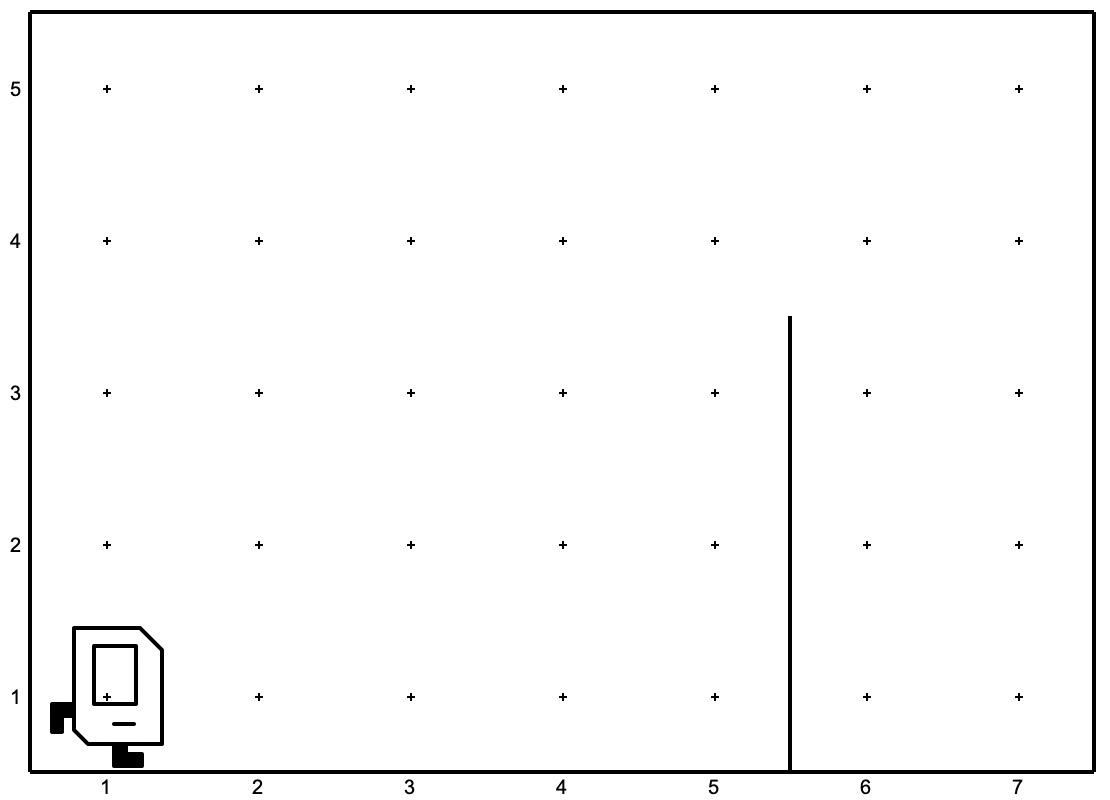
\includegraphics[scale=\figscale]{images/ch03/to_the_top/to_the_top_pre.jpg}
        \caption{မတိုင်မီ အခြေအနေ}   
        \label{fig:to_the_top_pre}
    \end{subfigure}
    \begin{subfigure}[t]{{\figpctw}\textwidth}
        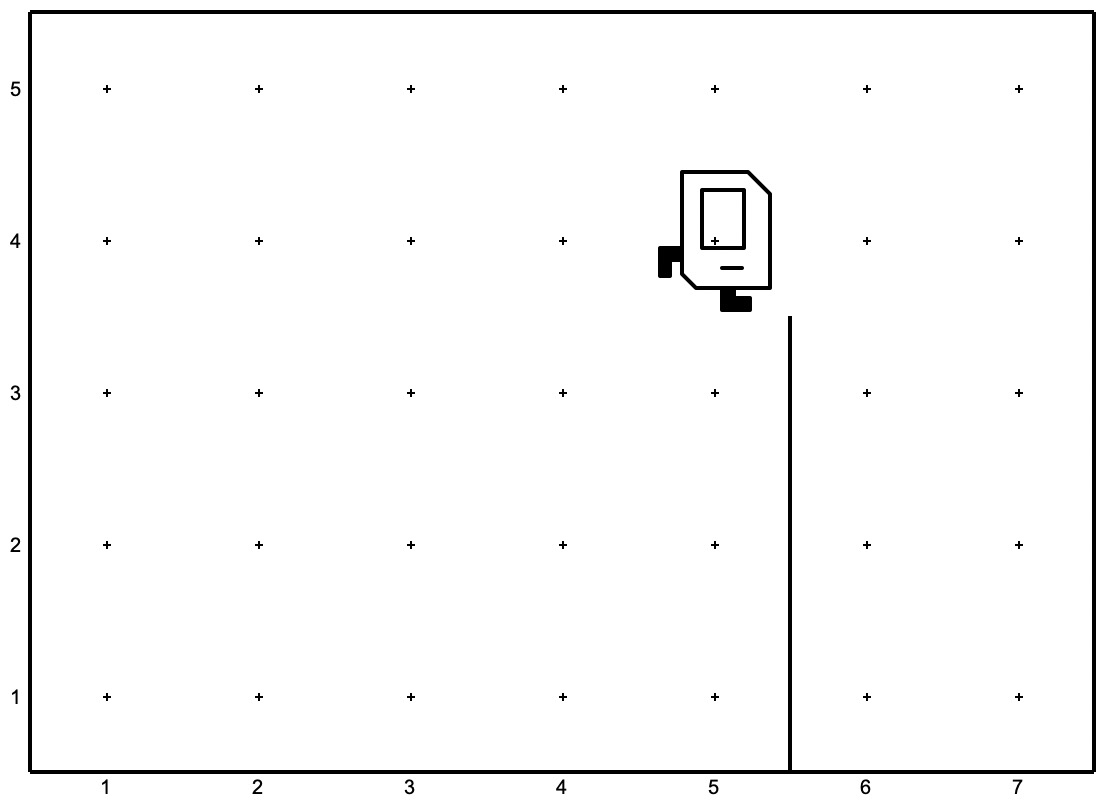
\includegraphics[scale=\figscale]{images/ch03/to_the_top/to_the_top_post.jpg}
        \caption{ပြီးနောက် အခြေအနေ} 
        \label{fig:to_the_top_post}   
    \end{subfigure}
    \caption{တိုင်ထိပ်သို့}
    \label{fig:to_the_top}
\end{figure}
%
တိုင်အောက်ခြေကိုသွားတာနဲ့ တိုင်ထိပ်တက်တာ အလုပ်နှစ်ခု ပါဝင်တယ်လို့ မြင်နိုင်တယ်။ ဒီအတွက် ဖန်ရှင်နှစ်ခု သတ်မှတ်ပေးပါမယ်။
%
\begin{py}
def go_to_pole():
    while front_is_clear():
        move()
\end{py}
%
%
\begin{py}
def ascend_pole():
    while right_is_blocked():
        move()
\end{py}
%
အထက်ပါ ဖန်ရှင်နှစ်ခုနဲ့ \fCode{go\_to\_top} ကို ဆက်လက် သတ်မှတ်ပါမယ်
%
\begin{py}
def go_to_top():
    go_to_pole()
    turn_left()
    ascend_pole()
    turn_right()
\end{py}
%
\fCode{go\_to\_pole} အပြီးမှာ ကားရဲလ်ဟာ တိုင်ခြေမှာ အရှေ့ဘက်မျက်နှာမူပြီး ရှိနေမှာပါ။ \fCode{ascend\_pole} က တိုင်ခြေမှာ ကားရဲလ် အပေါ်ဘက်ကို မျက်နှာမူတဲ့ အနေအထားကနေ စရပါမယ်။ \fCode{go\_to\_pole} ပြီးရင် \fCode{ascend\_pole} အတွက် အသင့်အနေအထားဖြစ်အောင် \fCode{turn\_left} လုပ်ပေးရပါမယ်။

ဖန်ရှင် စတင်မလုပ်ဆောင်မီ ကြိုတင်ရှိနေရမဲ့ အခြေအနေကို ပရီကွန်ဒီရှင်လို့ ပြောခဲ့ပါတယ်။ ဖန်ရှင် သတ်မှတ်တဲ့အခါ ပရီကွန်ဒီရှင်ကို တိတိကျကျ စဉ်းစားဖို့ လိုပါတယ်။ ဖန်ရှင်အသုံးပြုတဲ့အခါမှာလည်း သတ်မှတ်ထားတဲ့ ပရီကွန်ဒီရှင် အတိုင်းကိုက်ညီဖို့ လိုတယ်။ \fCode{ascend\_pole} ပရီကွန်ဒီးရှင်းဟာ တိုင်ခြေမှာ ကားရဲလ် အပေါ်ဘက်ကို မျက်နှာမူတဲ့ အနေအထား ဖြစ်ပါတယ်။ ပုံ \fRefNo{\ref{fig:mutp_pre_and_post}} (\fRefNo{\subref{fig:mutp_pre1}}) ကို ကြည့်ပါ။ %အကယ်၍ အဲဒီအတိုင်းမဟုတ်ရင် မက်သဒ်ကလည်း မှန်ကန်ကောင် လုပ်ဆောင်ပေးနိုင်ဖို့ မသေချာနိုင်ပါဘူး။

ဖန်ရှင် လုပ်ဆောင်အပြီးမှာ ရှိနေရမဲ့ အခြေအနေကို ပို့စ်ကွန်ဒီရှင်လို့ ဖော်ပြခဲ့တယ်။ ဖန်ရှင်တစ်ခုဟာ ပရီကွန်ဒီရှင်နဲ့ ကိုက်ညီတဲ့ အနေအထားကနေ စတင်ရင် ပို့စ်ကွန်ဒီရှင်နဲ့ ကိုက်ညီအောင်လုပ်ဆောင်ပေးပြီး အဆုံးသတ်ရမှာပါ။ ပုံ \fRefNo{\ref{fig:mutp_pre_and_post}} (\fRefNo{\subref{fig:mutp_post}}) မှာ \fCode{ascend\_pole} ပို့စ်ကွန်ဒီရှင်ကို တွေ့နိုင်ပါတယ်။
%
\begin{figure}[htb!]
    \hfuzz=100pt
    \newcommand{\figpctw}{0.52}
    \newcommand{\figscale}{0.165}
    \begin{subfigure}[t]{{\figpctw}\textwidth}
        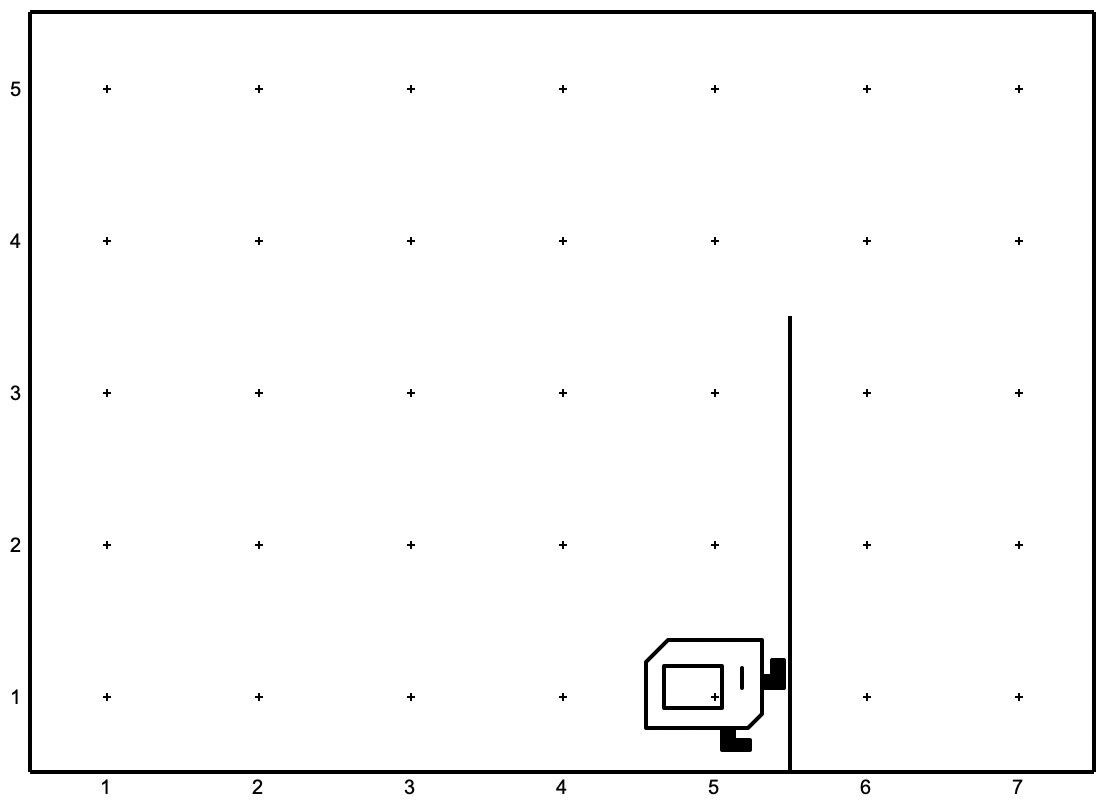
\includegraphics[scale=\figscale]{images/ch03/to_the_top/move_up_the_pole_pre1.jpg}
        \caption{}   
        \label{fig:mutp_pre1}
    \end{subfigure}
    \begin{subfigure}[t]{{\figpctw}\textwidth}
        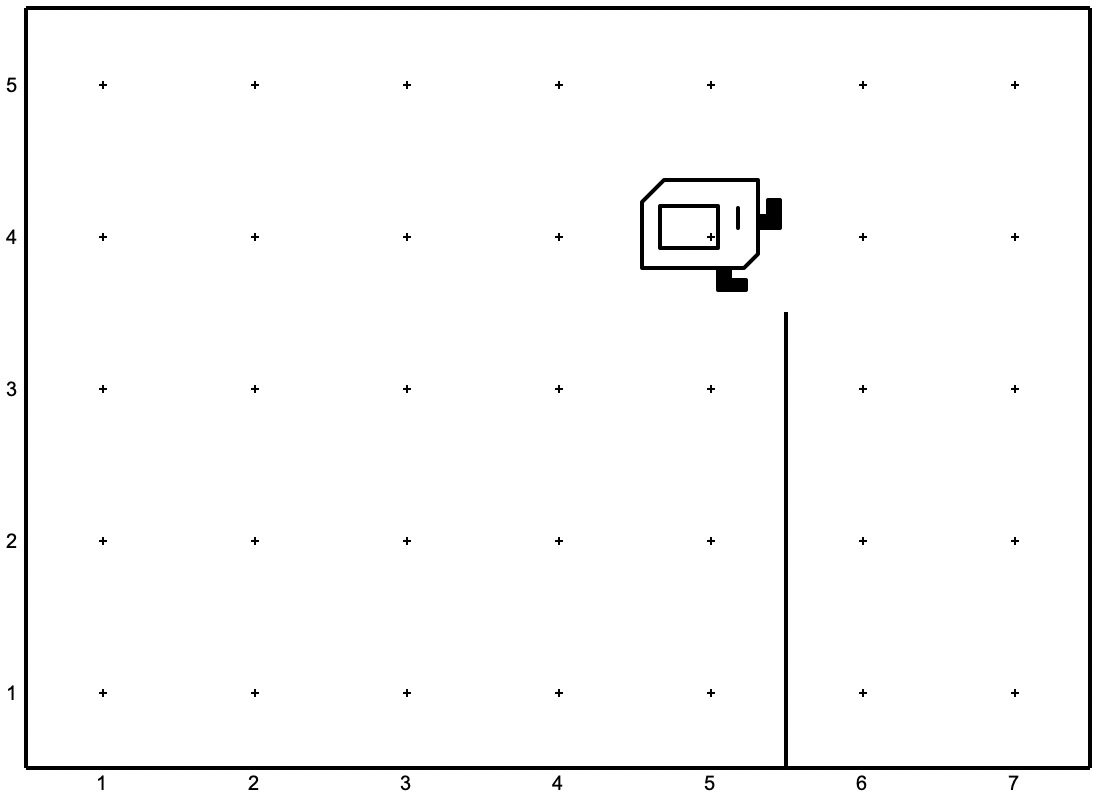
\includegraphics[scale=\figscale]{images/ch03/to_the_top/move_up_the_pole_post1.jpg}
        \caption{} 
        \label{fig:mutp_post}   
    \end{subfigure}
    \caption{\fCptCodeBf{ascend\_pole} ပရီကွန်ဒီးရှင်းနှင့် ပို့စ်ကွန်ဒီးရှင်း}
    \label{fig:mutp_pre_and_post}
\end{figure}


ဖန်ရှင် ပရီကွန်ဒီရှင် ပို့စ်ကွန်ဒီရှင်ကို သင့်တော်သလို သတ်မှတ်နိုင်ပါတယ်။ ပုံ (\fRefNo{\ref{fig:mutp_pre_and_post_v2}}) တွင် \fCode{ascend\_\allowbreak pole} အတွက် အခြား ရွေးချယ်နိုင်တဲ့ ပရီ နဲ့ ပို့စ် ကွန်ဒီရှင်ကို  ကြည့်ပါ။

\begin{figure}[tbh!]
    \hfuzz=100pt
    \newcommand{\figpctw}{0.52}
    \newcommand{\figscale}{0.165}
    \begin{subfigure}[t]{{\figpctw}\textwidth}
        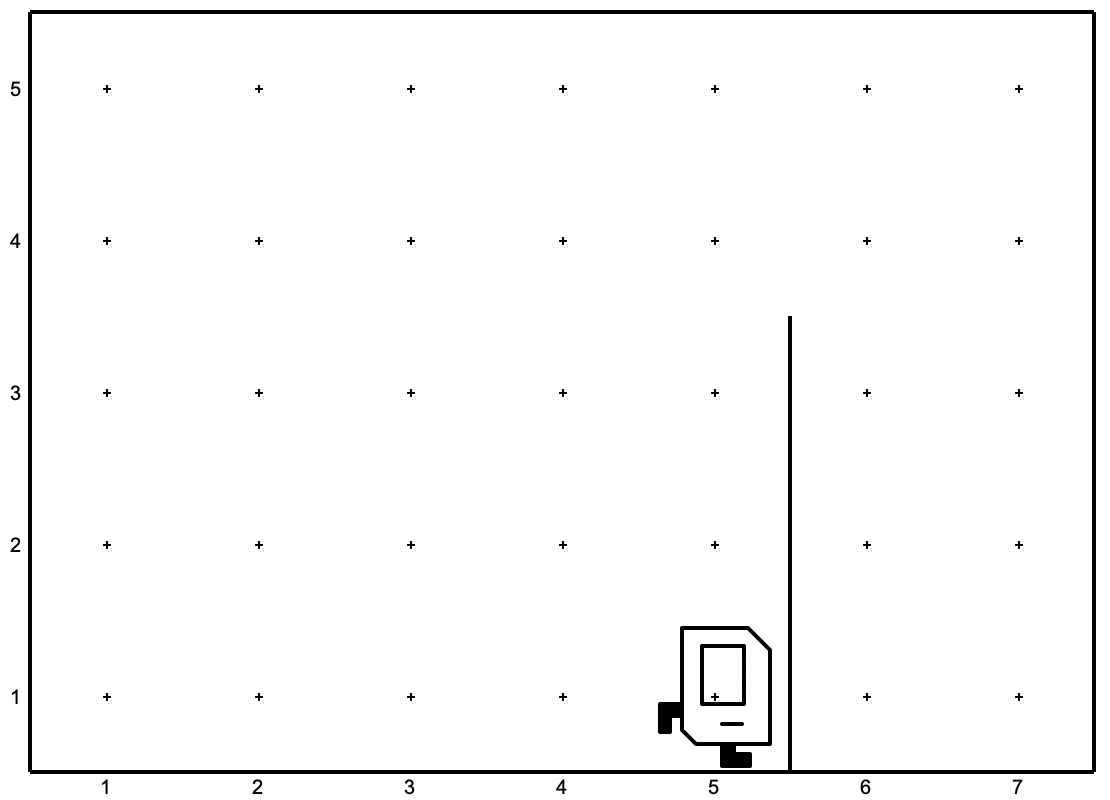
\includegraphics[scale=\figscale]{images/ch03/to_the_top/move_up_the_pole_pre_v2.jpg}
        \caption{}   
        \label{fig:mutp_pre_v2}
    \end{subfigure}
    \begin{subfigure}[t]{{\figpctw}\textwidth}
        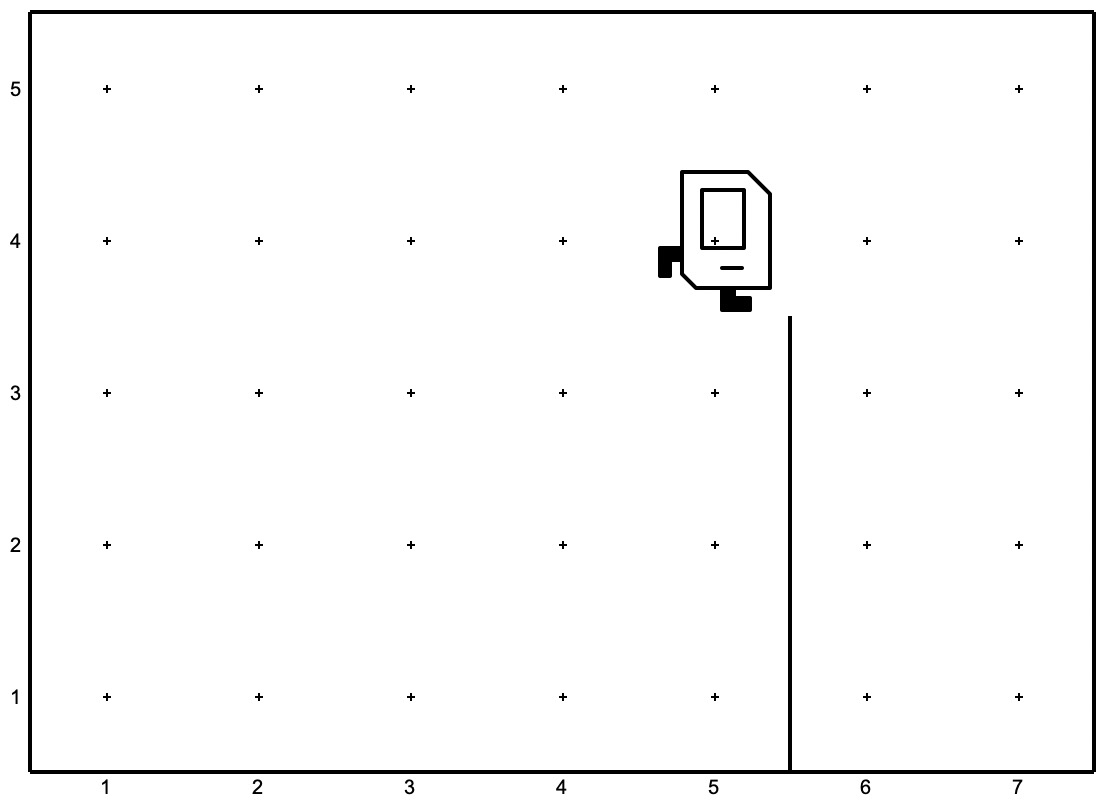
\includegraphics[scale=\figscale]{images/ch03/to_the_top/move_up_the_pole_post_v2.jpg}
        \caption{} 
        \label{fig:mutp_post_v2}   
    \end{subfigure}
    \caption{\fCptCodeBf{ascend\_pole} ပရီ နဲ့ ပို့စ် ကွန်ဒီရှင်}
    \label{fig:mutp_pre_and_post_v2}
\end{figure}

အထက်ပါ ပရီ နဲ့ ပို့စ် ကွန်ဒီရှင်အရ \fCode{ascend\_pole} ကို အခုလို 
%
\begin{py}
def ascend_pole():
    turn_left()
    while right_is_blocked():
        move()
    turn_right()
\end{py}
%
သတ်မှတ်ရမှာပါ။ \fCode{go\_to\_top} ကလည်း ဒီလို ဖြစ်သွားမယ်
%
\begin{py}
def go_to_top():
    go_to_pole()
    ascend_pole()
\end{py}
%

\section{ဖန်ရှင်များဖြင့် abstraction များ တည်ဆောက်ခြင်း}
အခန်း (\fRefNo{\ref{ch:ch02}}) စာမျက်နှာ (\fRefNo{\pageref{lst:repair_street}}) မှ လမ်းပြင်တဲ့ ပရိုဂရမ်မှာ ကွန်နာတစ်ခုဟာ ဘိပါလည်းမရှိ၊ အောက်ဘက်ကပ်လျက် နံရံလည်းမရှိရင်  ဘိပါတစ်ခု ချထားပေးရပါတယ်။ ဒီကိစ္စ ဆောင်ရွက်ပေးဖို့အတွက် ဖန်ရှင်တစ်ခု သတ်မှတ်နိုင်ပါတယ်။ 
%
\begin{figure}[htb!]
    {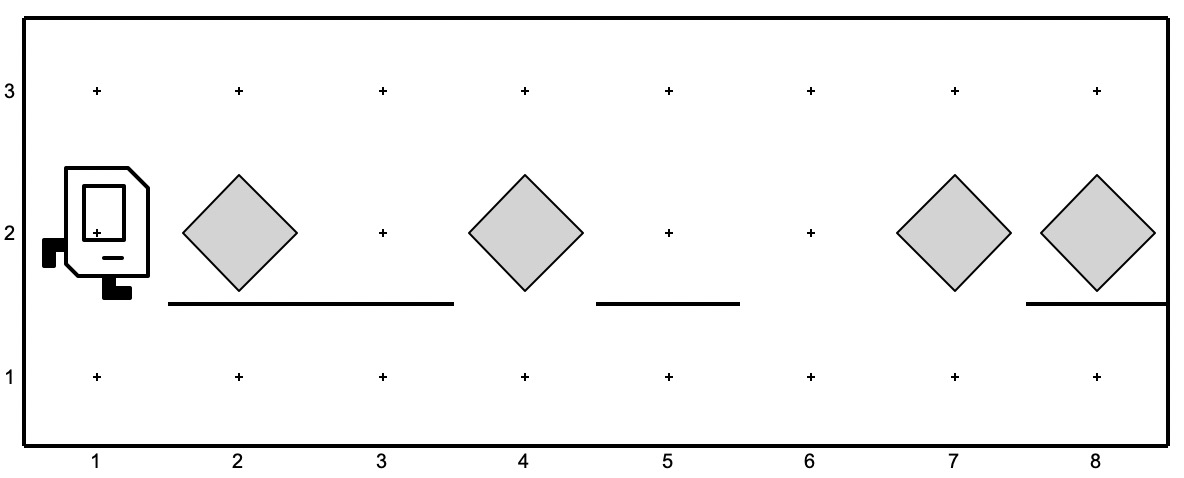
\includegraphics[width=0.5\linewidth]{images/ch02/st_repair/init.jpg}}
    \caption{}
\end{figure}
%
%
\begin{py}
def repair_corner():
    if right_is_clear():
        if no_beepers_present():
            put_beeper()
\end{py}
%
အခြေအနေနှစ်ခုစလုံး မှန်တော့မှ ဘိပါချပေးဖို့ \fEn{nested} \fCode{if}  သုံးထားတာက နားလည်ရ အတန်အသင့် ခက်ခဲနိုင်ပါတယ်။  ဒါပေမဲ့ \fCode{repair\_corner} ကို အသုံးပြုတဲ့အခါ ဘယ်လိုရေးထားလဲ စဉ်းစားစရာ မလိုပါဘူး။ ဘိပါလည်းမရှိ၊ ညာဘက် နံရံလည်းမရှိတဲ့ ကွန်နာမှာ ဘိပါချချင်ရင် \fCode{repair\_corner} ဖန်ရှင်နဲ့ လုပ်လို့ရတယ်ဆိုတာ သိထားရင် သုံးလို့ရပြီ။

ဖန်ရှင် သတ်မှတ်တဲ့အခါ ဆောင်ရွက်ပေးစေချင်တဲ့ ကိစ္စကို ‘ဘယ်လို လုပ်ရမှာလဲ’ အသေးစိတ် စဉ်းစားရမှာဖြစ်ပေမဲ့ အသုံးပြုတဲ့အခါမှာတော့ ဒီလိုအသေးစိတ်တွေကို ထပ်ပြီး စဉ်းစားဖို့ မလိုတော့ပါဘူး။ ဖန်ရှင် ‘ဘာလုပ်ပေးတာလဲ’ ကပဲ အရေးကြီးတယ်။ ‘ဘယ်လို’ တည်ဆောက်ထားလဲ သိစရာမလိုဘဲ ‘ဘာ’ လုပ်ပေးလဲ သိရုံနဲ့ အသုံးပြုလို့ရစေတာကို \fEn{abstraction} လုပ်တယ်လို့ခေါ်ပါတယ်။ \fEn{Abstraction} လုပ်ခြင်းအတွက် ဖန်ရှင်တွေဟာ အဓိက အကျဆုံး အခြေခံ အုတ်ချပ်တွေပါပဲ။ 


\fEn{Abstraction} လုပ်ထားလိုက်ခြင်းအားဖြင့် ရှုပ်ရှုပ်ထွေးထွေးတွေ ထပ်ခါထပ်ခါ ခေါင်းရှုပ်ခံ စဉ်းစားနေဖို့ မလိုအပ်တော့ဘဲ ကိစ္စတစ်ခုကို အလွယ်တကူ လုပ်ဆောင်လို့ရသွားတယ်။ ကုဒ်တွေဖတ်ရတာလည်း ပိုရှင်းပြီး နားလည်ရ လွယ်ကူသွားတယ်။ ဒါကြောင့် ပရိုဂရမ်တွေ တည်ဆောက်ရာမှာ \fEn{abstraction} လုပ်ခြင်းဟာ အရေးပါပါတယ်။ အရေးကြီးဆုံးလို့ ဆိုရင်လည်း မမှားဘူး။  ကြီးမားရှုပ်ထွေးတဲ့ ဆော့ဖ်ဝဲတွေကို လေ့လာကြည့်ရင်  \fEn{abstraction} ပေါင်းများစွာနဲ့ တစ်ဆင့်ပြီးတစ်ဆင့်၊ တစ်လွှာပြီးတစ်လွှာ တည်ဆောက်ထားတယ်ဆိုတာ တွေ့ရမှာပါ။

\fCode{repair\_corner} ဟာ အနိမ့်ဆုံးအလွှာက အခြေခံ \fEn{abstraction} တစ်ခု ဖြစ်တယ် ဆိုပါစို့။ ၎င်းကို အခြေခံပြီး တစ်ဆင့်ပိုမြင့်တဲ့ အလွှာအတွက် \fEn{abstraction} တွေကို တည်ဆောက်ယူနိုင်ပါတယ်။ ဥပမာ
%
\begin{py}
def repair_street():
    while front_is_clear():
        repair_corner()
    repair_corner()
\end{py}
%
ဒီအလွှာထက် နောက်ထပ် တစ်ဆင့်ပိုမြင့်တဲ့ \fEn{abstraction} တွေကိုလည်း ဆက်လက် တည်ဆောက်ယူနိုင်ပါတယ်။ ဥပမာ \fCode{repair\_world} ကို တည်ဆောက်ရာမှာ \fCode{repair\_street} ကို အခြေခံအစိတ်အပိုင်းအဖြစ် အသုံးပြုနိုင်ပါတယ်။ ဒီလို \fEn{abstraction} အလွှာတွေ အဆင့်ဆင့်နဲ့ ပရိုဂရမ် တည်ဆောက်နည်း တွေကို ဆက်လက်လေ့လာကြရပါမယ်။


\section{Bottom-up Programming}

ကြီးကျယ်ခမ်းနားတဲ့ အဆောက်အအုံကြီးတွေ၊ လျှို့ဝှက်ဆန်းကြယ်တဲ့ သဘာဝဖြစ်စဉ်တွေ၊ အံ့ဖွယ်သိပ္ပံနှင့် နည်းပညာ ဆန်းသစ်တီထွင်မှုတွေ စတဲ့အရာတွေအားလုံးဟာ ရိုးရှင်းတဲ့ အစိတ်အပိုင်းလေးတွေနဲ့ ဖွဲ့စည်းထားတာပါပဲ။ ဒါကြောင့် အရွယ်အစား ကြီးမား ရှုပ်ထွေးတဲ့ ပရိုဂရမ်တွေကိုလည်း ရိုးရှင်းတဲ့ အစိတ်အပိုင်းလေးတွေနဲ့ အခြေပြု ဖွဲ့စည်းတည်ဆောက်သင့်တယ်လို့ ယူဆမယ်ဆိုရင် ကျိုးကြောင်းဆီလျော်တယ်ပဲ ဆိုရမှာပါ။

ခက်ခဲရှုပ်ထွေးတဲ့ ကိစ္စတစ်ခုကို ဖြေရှင်းတဲ့အခါ အပိုင်းတွေခွဲပြီး တစ်ပိုင်းချင်းကို သီးခြားဖြေရှင်းလေ့ရှိတယ်။ အပိုင်းတွေခွဲလိုက်ခြင်းအားဖြင့် တစ်ပိုင်းစီဟာ မူလဖြေရှင်းရမဲ့ ကိစ္စလောက် မခက်ခဲတော့ပါဘူး။ အရွယ်အစားအားဖြင့်လည်း နဂိုထက် ငယ်သွားမယ်။ အပိုင်း တစ်ပိုင်းချင်းစီကို ဖြေရှင်းတဲ့အခါမှာလည်း အလားတူပဲ လုပ်ဆောင်နိုင်တယ်။ အပိုင်းတစ်ပိုင်းကို သူ့ထက်သေးငယ်တဲ့ အပိုင်းတွေအဖြစ် ထပ်မံခွဲထုတ်နိုင်ပါတယ်။ ဒီတိုင်း တစ်ဆင့်ပြီးတစ်ဆင့် လုပ်သွားမယ်ဆိုရင် နောက်ဆုံးမှာ အလွယ်တကူဖြေရှင်းလို့ရတဲ့ အစိတ်အပိုင်းလေးတွေ ဖြစ်သွားရမှာပါပဲ။ \fEnEmp{Bottom-up programming} ဆိုတာကတော့ ပရိုဂရမ်ရေးပြီး ကိစ္စတစ်ခုကို ဖြေရှင်းရာမှာ ရိုးရှင်းသထက်ရိုးရှင်း၊ သေးငယ်သထက်သေးငယ်တဲ့ အပိုင်းလေးတွေဖြစ်လာအောင် အဆင့်ဆင့်ပိုင်းခွဲပြီး အောက်ခြေအရိုးရှင်းဆုံးအလွှာကနေ အပေါ်ကိုတစ်ဆင့်ချင်းတက် ဖြေရှင်းတဲ့နည်း ဖြစ်တယ်။ လေ့လာကြည့်ကြရအောင်။

ပုံ (\fRefNo{\ref{fig:hurdle_jumping_init}}) ကမ္ဘာမှာ ကားရဲလ် တန်းကျော်ပြေးပြိုင်ရပါမယ်။ ထောင်လိုက်နံရံတွေကို တန်းတွေလို့ယူဆပါ။ တန်းတွေဟာ အနိမ့်အမြင့် အမျိုးမျိုးဖြစ်နိုင်ပါတယ်။ ကမ္ဘာရဲ့ အပေါ်ဘက် နံရံကို ထိတဲ့အထိတော့ မြင့်လို့မရပါဘူး။ ဒါမှ တန်းကိုကျော်ပြီး အခြားဘက်ကို သွားလို့ရမှာပါ။ \((1, 1)\) ကွန်နာကနေ တာစထွက်မှာဖြစ်ပြီး \((14, 1)\) မှာ ပန်းဝင်ရမှာပါ။
%
\begin{figure}[htb!]
    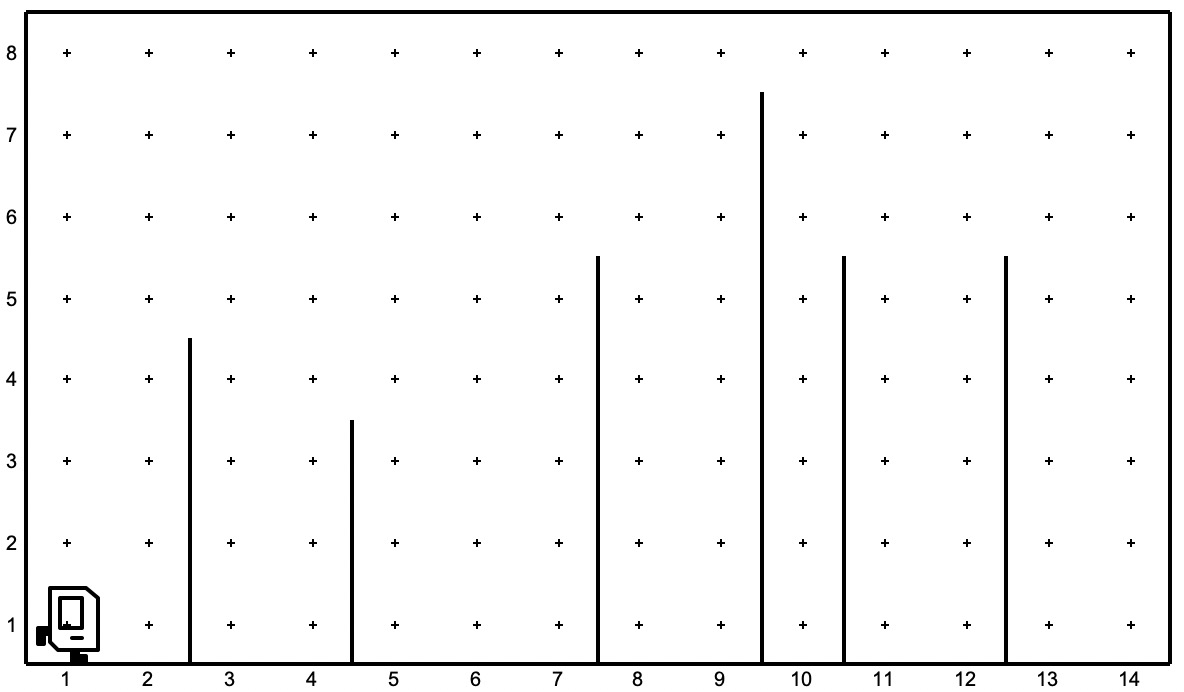
\includegraphics[width=4.5in]{images/ch03/hurdle_jumping/init_w1.jpg}
    \caption{}
    \label{fig:hurdle_jumping_init}
\end{figure}
%

တန်းကျော်ပြေးတဲ့ ကိစ္စမှာ ပါဝင်တဲ့ အပိုင်းတစ်ခုက တန်းတစ်ခုကျော်တာ။ တန်းတစ်ခု ကျော်တာကို ထပ်ခွဲကြည့်ရင် အပေါ်တက်တာနဲ့ အောက်ဆင်းတာ နှစ်ပိုင်းရှိမယ်။ အခုလို နဂိုမူလကိစ္စတစ်ခုကနေ တစ်ဆင့်ထက်တစ်ဆင့် ပိုသေးငယ်တဲ့ အပိုင်းလေးတွေဖြစ်လာအောင် ခွဲထုတ်တာကို \fEnEmp{problem decomposition} လုပ်တယ်လို ခေါ်ပါတယ်။ 

\fEn{Bottom-up programming} နည်းနဲ့ ပရိုဂရမ်ရေးတဲ့အခါ \fEn{problem decomposition} အရင်ဦးဆုံး  လုပ်ရတယ်။ ပြီးရင် အောက်ဆုံးအလွှာမှ အသေးဆုံးအပိုင်းလေးတွေကနေ စတင်ဖြေရှင်းတယ်။ ပြီးတဲ့အခါ အဲဒီ အသေးဆုံး အပိုင်းလေးတွေကို အခြေခံအစိတ်အပိုင်းအဖြစ် အသုံးပြုပြီး  အောက်ဆုံးအလွှာထက် တစ်ဆင့်မြင့်တဲ့ အပေါ်အလွှာက အပိုင်းတွေကို ဆက်လက်ဖြေရှင်းတယ်။ ဒီအလွှာက အပိုင်းတွေကို  အခြေခံအစိတ်အပိုင်းအဖြစ် အသုံးပြုပြီး နောက်ထပ်တစ်ဆင့် ပိုမြင့်တဲ့အလွှာက အပိုင်းတွေကို ဆက်လက်ဖြေရှင်းမှာဖြစ်တယ်။ ဒီလိုမျိုး အောက်ကနေ အပေါ်ကို တစ်လွှာပြီးတစ်လွှာ တက်သွားပြီး ဖြေရှင်းတဲ့ နည်းစနစ်ဟာ \fEn{bottom-up programming} ပါပဲ။ 

တန်းကျော်ပြေးပွဲမှာ \fEn{Problem Decomposition} လုပ်ထားတာကို တစ်လွှာချင်း ခွဲကြည့်မယ်ဆိုရင် အခုလိုတွေ့ရမှာ ဖြစ်ပါတယ်။
%
\begin{itemize}
  \item တန်းကျော်ပြေးပြိုင်ပွဲဝင်ခြင်း
  \begin{itemize}
    \item တန်းတစ်ခုကျော်ခြင်း
    \begin{itemize}
      \item အပေါ်တက်ခြင်း
      \item အောက်ဆင်းခြင်း
    \end{itemize}
  \end{itemize} 
\end{itemize}
%
\fEn{Bottom-up} နည်းအရ အောက်ဆုံးအလွှာ အပေါ်တက်၊ အောက်ဆင်း ကိစ္စကို ပထမဆုံး ဖြေရှင်းပါမယ်။ အပိုင်းတစ်ခုအတွက် ဖန်ရှင်တစ်ခု သတ်မှတ်ရပါမယ်။

%
\begin{py}
def ascend():
    ß\PYG{l+s+sd}{\PYGZdq{}\PYGZdq{}\PYGZdq{}}ß
    ß\PYG{l+s+sd}{\fMM{တန်းနဲ့လွတ်တဲ့အထိ အပေါ်သို့ တက်သည်}}ß
    ß\PYG{l+s+sd}{\fEnEmp{Precondition:} \fMM{တန်းဘယ်ဘက် ခြေရင်းမှာ အရှေ့ဘက်မျက်နှာမူပြီး ရှိနေ}}ß
    ß\PYG{l+s+sd}{\fEnEmp{Postcondition:} \fMM{တန်းထိပ်အပေါ် ဘယ်ဘက်ကွန်နာမှာ အရှေ့ဘက်မျက်နှာမူပြီး ရှိနေ}}ß
    ß\PYG{l+s+sd}{\PYGZdq{}\PYGZdq{}\PYGZdq{}}ß
    turn_left()
    while right_is_blocked():
        move()
    turn_right()
\end{py}
%
%
\begin{py}
def descend():
    ß\PYG{l+s+sd}{\PYGZdq{}\PYGZdq{}\PYGZdq{}}ß
    ß\PYG{l+s+sd}{\fMM{တန်းအောက်သို့ ပြန်ဆင်းသည်}}ß
    ß\PYG{l+s+sd}{\fEnEmp{Precondition:} \fMM{တန်းထိပ်အပေါ် ညာဘက်ကွန်နာမှာ အရှေ့ဘက်မျက်နှာမူပြီး ရှိနေ}}ß
    ß\PYG{l+s+sd}{\fEnEmp{Postcondition:} \fMM{တန်းညာဘက် ခြေရင်းမှာ အရှေ့ဘက်မျက်နှာမူပြီး ရှိနေ}}ß
    ß\PYG{l+s+sd}{\PYGZdq{}\PYGZdq{}\PYGZdq{}}ß
    turn_right()
    while front_is_clear():
        move()
    turn_left()
\end{py}
%

အထက်ပါ ဖန်ရှင်နှစ်ခုကို အသုံးပြုပြီး အပေါ်တစ်ဆင့် ပိုမြင့်တဲ့ အလွှာက တန်းတစ်ခုကျော်တာကို ဆက်လက်ဖြေရှင်းရပါမယ်။ \fCode{ascend} နဲ့ \fCode{descend} ပရီနဲ့ ပို့စ် ကွန်ဒီရှင်တွေအရ \fCode{move} လုပ်ပေးဖို့လိုပါတယ်။
%
\begin{py}
def jump_over_hurdle():
    ß\PYG{l+s+sd}{\PYGZdq{}\PYGZdq{}\PYGZdq{}}ß
    ß\PYG{l+s+sd}{\fMM{တန်းတစ်ခုကို ကျော်သည်}}ß
    ß\PYG{l+s+sd}{\fEnEmp{Precondition:} \fMM{တန်းဘယ်ဘက် ခြေရင်းမှာ အရှေ့ဘက်မျက်နှာမူပြီး ရှိနေ}}ß
    ß\PYG{l+s+sd}{\fEnEmp{Postcondition:} \fMM{တန်းညာဘက် ခြေရင်းမှာ အရှေ့ဘက်မျက်နှာမူပြီး ရှိနေ}}ß
    ß\PYG{l+s+sd}{\PYGZdq{}\PYGZdq{}\PYGZdq{}}ß
    ascend()
    move()
    descend()
\end{py}
%

ဒီဖန်ရှင်နဲ့ နောက်တစ်ဆင့်ကို ဆက်လက်တည်ဆောက်ရပါမယ်။ ရှေ့မှာရှင်းနေလျှင် ရှေ့တိုးမယ်၊ မရှင်းလျှင် တန်းကိုကျော်ရမယ်။ ပန်းဝင်ဖို့အတွက်ဆိုလျှင် ဒီအလုပ်ကို ဆယ့်သုံးခါလုပ်ပေးရုံပါပဲ။
%
\begin{py}
def compete_hurdle_race():
    ß\PYG{l+s+sd}{\PYGZdq{}\PYGZdq{}\PYGZdq{}}ß
    ß\PYG{l+s+sd}{\fMM{တန်းကျော်ပြေးပြိုင်ပွဲ ပန်းဝင်သည်ထိ ယှဉ်ပြိုင်သည်}}ß
    ß\PYG{l+s+sd}{\fEnEmp{Precondition:} \fMM{(၁,၁) ကွန်နာတွင် အရှေ့ဘက်မျက်နှာမူနေ}}ß
    ß\PYG{l+s+sd}{\fEnEmp{Postcondition:} \fMM{(၁၄,၁) ကွန်နာတွင် အရှေ့ဘက်မျက်နှာမူနေ}}ß
    ß\PYG{l+s+sd}{\PYGZdq{}\PYGZdq{}\PYGZdq{}}ß
    for i in range(13):
        if front_is_clear():
            move()
        else:
            jump_over_hurdle()
\end{py}
%

ပရိုဂရမ် အစအဆုံးကို လေ့လာကြည့်ပါ။ ဖန်ရှင်တစ်ခုချင်း ပရီနဲ့ ပို့စ် ကွန်ဒီရှင်တွေကို တိတိကျကျ မြင်အောင် ဂရုစိုက်ကြည့်ဖို့လည်း အရေးကြီးတယ်။ ဖန်ရှင် \fEn{docstring} မှာ ၎င်းဖန်ရှင် ပရီနဲ့ ပို့စ် ကွန်ဒီရှင်ကို တိတိကျကျ ဖော်ပြထားတာဟာ အလေ့အထကောင်း တစ်ခုပါ။ ဖန်ရှင်တိုင်းမှာ ပါသင့်တယ်။

%
\begin{py}
# File: hurdle_jumping.py
from stanfordkarel import *


def main():
    """Hurdle Jumping Program"""
    compete_hurdle_race()


def ascend():
    ß\PYG{l+s+sd}{\PYGZdq{}\PYGZdq{}\PYGZdq{}}ß
    ß\PYG{l+s+sd}{\fMM{တန်းနဲ့လွတ်တဲ့အထိ အပေါ်သို့ တက်သည်}}ß
    ß\PYG{l+s+sd}{\fEnEmp{Precondition:} \fMM{တန်းဘယ်ဘက် ခြေရင်းမှာ အရှေ့ဘက်မျက်နှာမူပြီး ရှိနေ}}ß
    ß\PYG{l+s+sd}{\fEnEmp{Postcondition:} \fMM{တန်းထိပ်အပေါ် ဘယ်ဘက်ကွန်နာမှာ အရှေ့ဘက်မျက်နှာမူပြီး ရှိနေ}}ß
    ß\PYG{l+s+sd}{\PYGZdq{}\PYGZdq{}\PYGZdq{}}ß
    turn_left()
    while right_is_blocked():
        move()
    turn_right()


def descend():
    ß\PYG{l+s+sd}{\PYGZdq{}\PYGZdq{}\PYGZdq{}}ß
    ß\PYG{l+s+sd}{\fMM{တန်းအောက်သို့ ပြန်ဆင်းသည်}}ß
    ß\PYG{l+s+sd}{\fEnEmp{Precondition:} \fMM{တန်းထိပ်အပေါ် ညာဘက်ကွန်နာမှာ အရှေ့ဘက်မျက်နှာမူပြီး ရှိနေ}}ß
    ß\PYG{l+s+sd}{\fEnEmp{Postcondition:} \fMM{တန်းညာဘက် ခြေရင်းမှာ အရှေ့ဘက်မျက်နှာမူပြီး ရှိနေ}}ß
    ß\PYG{l+s+sd}{\PYGZdq{}\PYGZdq{}\PYGZdq{}}ß
    turn_right()
    while front_is_clear():
        move()
    turn_left()


def jump_over_hurdle():
    ß\PYG{l+s+sd}{\PYGZdq{}\PYGZdq{}\PYGZdq{}}ß
    ß\PYG{l+s+sd}{\fMM{တန်းတစ်ခုကို ကျော်သည်}}ß
    ß\PYG{l+s+sd}{\fEnEmp{Precondition:} \fMM{တန်းဘယ်ဘက် ခြေရင်းမှာ အရှေ့ဘက်မျက်နှာမူပြီး ရှိနေ}}ß
    ß\PYG{l+s+sd}{\fEnEmp{Postcondition:} \fMM{တန်းညာဘက် ခြေရင်းမှာ အရှေ့ဘက်မျက်နှာမူပြီး ရှိနေ}}ß
    ß\PYG{l+s+sd}{\PYGZdq{}\PYGZdq{}\PYGZdq{}}ß
    ascend()
    move()
    descend()


def compete_hurdle_race():
    ß\PYG{l+s+sd}{\PYGZdq{}\PYGZdq{}\PYGZdq{}}ß
    ß\PYG{l+s+sd}{\fMM{တန်းကျော်ပြေးပြိုင်ပွဲ ပန်းဝင်သည်ထိ ယှဉ်ပြိုင်သည်}}ß
    ß\PYG{l+s+sd}{\fEnEmp{Precondition:} \fMM{(၁,၁) ကွန်နာတွင် အရှေ့ဘက်မျက်နှာမူနေ}}ß
    ß\PYG{l+s+sd}{\fEnEmp{Postcondition:} \fMM{(၁၄,၁) ကွန်နာတွင် အရှေ့ဘက်မျက်နှာမူနေ}}ß
    ß\PYG{l+s+sd}{\PYGZdq{}\PYGZdq{}\PYGZdq{}}ß
    for i in range(13):
        if front_is_clear():
            move()
        else:
            jump_over_hurdle()


def turn_right():
    for i in range(3):
        turn_left()


if __name__ == "__main__":
    run_karel_program("hurdle_jumping")

\end{py}
%


\subsection*{အမှိုက်သိမ်းတဲ့ ကားရဲလ်}
အခုတစ်ခါမှာ ကားရဲလ်က အမှိုက်တွေရှင်းပေးရပါမယ်။ ပုံ (\fRefNo{\ref{fig:stw}}) နမူနာ ကမ္ဘာမှာ ကြုံရာကျပန်း \fEn{(random)} ပြန့်ကျဲနေတဲ့ ဘိပါတွေကို အမှိုက်လို့ ယူဆပါ။  ကမ္ဘာအရွယ်အစား အမျိုးမျိုးအတွက် အမှိုက်ရှင်းပေးတဲ့ ပရိုဂရမ်တစ်ခု ရေးပေးရမှာပါ။
\begin{figure}[htb!]
    {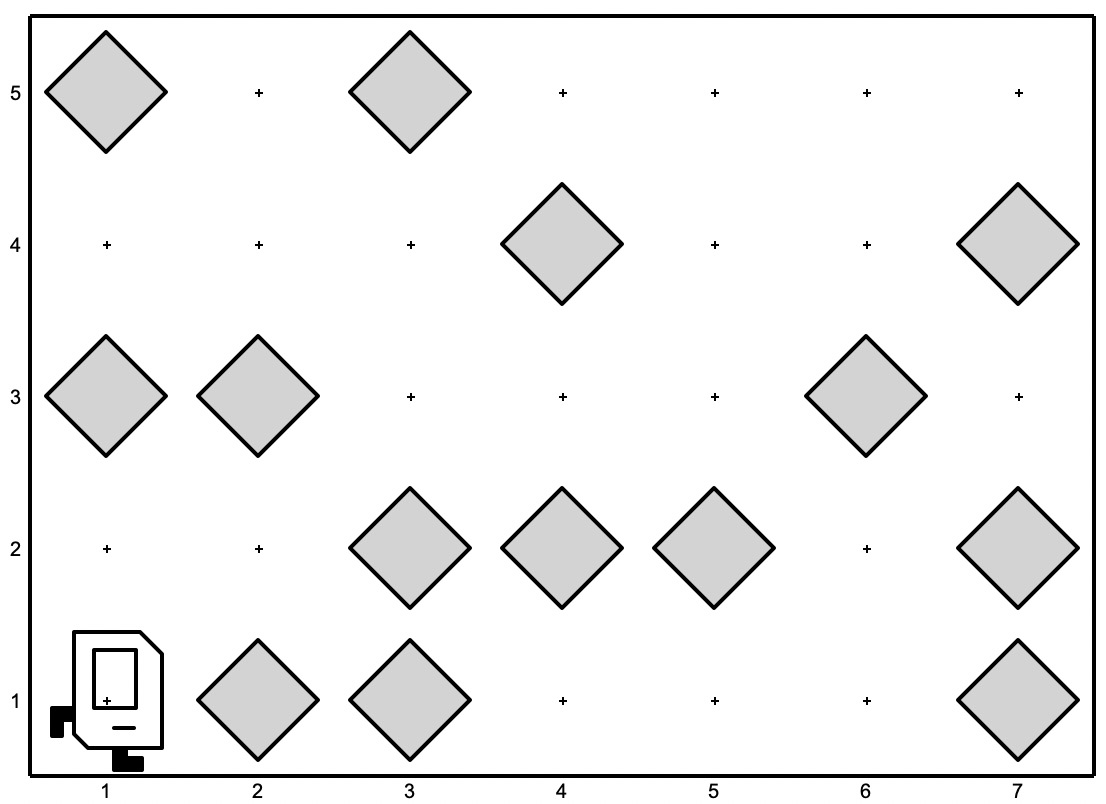
\includegraphics[width=.5\linewidth]{images/ch03/clean_the_world/init_w1.jpg}}
\caption{}
\label{fig:stw}
\end{figure}

ဒီကိစ္စကို ဖြေရှင်းဖို့က နည်းလမ်းတစ်ခုတည်း ရှိတာ မဟုတ်ပါဘူး။ နည်းလမ်းတစ်ခုက ဒီလိုပါ။ (၁) လမ်းကနေ စပြီး ရှင်းတယ် $\big\llbracket$စာမျက်နှာ \fRefNo{\pageref{fig:stw_alg1}} ပုံ (\fRefNo{\ref{fig:stw_alg1}}) (က) နှင့် (ခ) တွင် ကြည့်ပါ$\big\rrbracket$။ ပြီးရင် မြောက်ဘက် လှည့်ထားမယ် $\big\llbracket$ပုံ (\fRefNo{\ref{fig:stw_alg1}}) (ဂ)$\big\rrbracket$။ ရှင်းနေသေးတယ်ဆိုရင် ဒုတိယလမ်းကို တက်၊ အနောက်ဘက် မျက်နှာမူထားမယ် $\big\llbracket$ပုံ (\fRefNo{\ref{fig:stw_alg1}}) (ဃ)$\big\rrbracket$။ ဒုတိယလမ်းကို ဆက်ရှင်းပြီးတော့လည်း မြောက်ဘက်ကိုပဲ မျက်နှာမူထားပါမယ် $\big\llbracket$ပုံ (\fRefNo{\ref{fig:stw_alg1}}) (င)၊ (စ)$\big\rrbracket$။ ရှင်းနေသေးရင် တတိယလမ်းကို ကူး၊ အရှေ့ဘက်မျက်နှာ မူထားမယ် $\big\llbracket$ပုံ (\fRefNo{\ref{fig:stw_alg1}}) (ဆ)$\big\rrbracket$။ ဒီအတိုင်း တစ်လမ်းပြီးတစ်လမ်း ရှင်းသွားမှာဖြစ်တယ်။ လမ်းတစ်လမ်းရှင်းပြီး မြောက်ဘက်မျက်နှာမူလို့ ပိတ်နေရင် နောက်ထပ် လမ်းမရှိတော့ဘူး။ လမ်းအားလုံး ရှင်းပြီးသွားပြီ။ စာမျက်နှာ \fRefNo{\pageref{fig:stw_alg1_last_st}} ပုံ (\fRefNo{\ref{fig:stw_alg1_last_st}}) (က)၊ (ခ)၊ (ဂ) တို့ကို ကြည့်ပါ။ \fEn{Problem decomposition} လုပ်ကြည့်ရင် အောက်ပါအတိုင်း တွေ့နိုင်ပါတယ်။ 

%
\begin{figure}[htb!]
    \hfuzz=100pt
    \newcommand{\figpctw}{0.52}
    \newcommand{\figscale}{0.165}
    \begin{subfigure}[t]{{\figpctw}\textwidth}
        %\adjincludegraphics[width=2.5in,trim={0 0 0 {.55\height}}, clip, left]{ch03/SweepTheStreets/init_w1.jpg}
        \adjincludegraphics[scale=\figscale, trim={0 3pt 0 10cm}, clip, left]{images/ch03/clean_the_world/alg1/stp1a.jpg}
        \caption{}
        \label{fig:fst_bef}
    \end{subfigure}
    \begin{subfigure}[t]{{\figpctw}\textwidth}
        \adjincludegraphics[scale=\figscale, trim={0 3pt 0 10cm}, clip, left]{images/ch03/clean_the_world/alg1/stp1b.jpg}
        \caption{}
        \label{fig:fst_aft}
    \end{subfigure}

    \begin{subfigure}[t]{{\figpctw}\textwidth}
        \adjincludegraphics[scale=\figscale, trim={0 3pt 0 10cm}, clip, left]{images/ch03/clean_the_world/alg1/stp2.jpg}
        \caption{}
        \label{fig:fst_tn}
    \end{subfigure}
    \begin{subfigure}[t]{{\figpctw}\textwidth}
        \adjincludegraphics[scale=\figscale, trim={0 3pt 0 10cm}, clip, left]{images/ch03/clean_the_world/alg1/stp3a.jpg}
        \caption{}
        \label{fig:xyz4}
    \end{subfigure}
    \begin{subfigure}[t]{{\figpctw}\textwidth}
        \adjincludegraphics[scale=\figscale, trim={0 3pt 0 10cm}, clip, left]{images/ch03/clean_the_world/alg1/stp3b.jpg}
        \caption{}
        \label{fig:xyz5}
    \end{subfigure}
    \begin{subfigure}[t]{{\figpctw}\textwidth}
        \adjincludegraphics[scale=\figscale, trim={0 3pt 0 10cm}, clip, left]{images/ch03/clean_the_world/alg1/stp4.jpg}
        \caption{}
        \label{fig:xyz6}
    \end{subfigure}
    \begin{subfigure}[t]{{\figpctw}\textwidth}
        \adjincludegraphics[scale=\figscale, trim={0 3pt 0 10cm}, clip, left]{images/ch03/clean_the_world/alg1/stp5a.jpg}
        \caption{}
        \label{fig:xyz7}
    \end{subfigure}
    \begin{subfigure}[t]{{\figpctw}\textwidth}
        \adjincludegraphics[scale=\figscale, trim={0 3pt 0 10cm}, clip, left]{images/ch03/clean_the_world/alg1/stp5b.jpg}
        \caption{}
        \label{fig:xyz8}
    \end{subfigure}
    \caption{}
    \label{fig:stw_alg1}
\end{figure}
%

%
\begin{figure}[htb!]
    %\adjincludegraphics[width=2.5in,trim={0 0 0 {.55\height}}, clip, left]{images/}
    \hfuzz=100pt
    \newcommand{\figpctw}{0.52}
    \newcommand{\figscale}{0.165}
    \begin{subfigure}[t]{{\figpctw}\textwidth}
        \adjincludegraphics[scale=\figscale, trim={0 15cm 0 0}, clip, left]{images/ch03/clean_the_world/alg1/stp6a.jpg}
        \caption{}
    \end{subfigure}
    \begin{subfigure}[t]{{\figpctw}\textwidth}
        \adjincludegraphics[scale=\figscale, trim={0 15cm 0 0}, clip, left]{images/ch03/clean_the_world/alg1/stp6b.jpg}
        \caption{}
    \end{subfigure}
    \begin{subfigure}[t]{{\figpctw}\textwidth}
        \adjincludegraphics[scale=\figscale, trim={0 15cm 0 0}, clip, left]{images/ch03/clean_the_world/alg1/stp7.jpg}
        \caption{}
    \end{subfigure}
    \caption{}
    \label{fig:stw_alg1_last_st}
\end{figure}
%

%
\begin{itemize} \label{fig:btmup_pd}
    \item ကမ္ဘာတစ်ခုလုံး အမှိုက်တွေရှင်း \fEn{(clean world)}
    %
    \begin{itemize}
        \item လမ်းတစ်လမ်း အမှိုက်ရှင်း  \fEn{(clean street)}     
        %
        \begin{itemize}
            \item ကွန်နာတစ်ခု အမှိုက်ရှင်း \fEn{(clean corner)}
        \end{itemize}
        %
        \item မြောက်ဘက်လှည့် \fEn{(turn north)}
        \item လမ်းပြောင်း/နောက်တစ်လမ်းကူး \fEn{(change street)}
    \end{itemize}
    %
\end{itemize}
%

လမ်းတစ်လမ်း ရှင်းတဲ့ ကိစ္စကို ထပ်ခွဲကြည့်ရင် ကွန်နာတစ်ခုရှင်းတာကို တွေ့ရမှာပါ။ \fEn{Bottom-up} နည်းအရ အောက်ဆုံးအလွှာက ကွန်နာတစ်ခု အမှိုက်ရှင်းတဲ့ ကိစ္စအတွက် ဖန်ရှင်ကို ပထမဆုံး သတ်မှတ်ရပါမယ်။
%
\begin{py}
def clean_corner():
    ß\PYG{l+s+sd}{\PYGZdq{}\PYGZdq{}\PYGZdq{}}ß
    ß\PYG{l+s+sd}{\fMM{ကွန်နာတစ်ခုမှာ ဘိပါရှင်းပေးသည်}}ß
    ß\PYG{l+s+sd}{\fEnEmp{Precondition:} \fMM{ကွန်နာတစ်ခုမှာ ကားရဲလ် ရှိနေမယ်။ အများဆုံး ဘိပါတစ်ခု ရှိနိုင်တယ်။}}ß
    ß\PYG{l+s+sd}{\fEnEmp{Postcondition:} \fMM{ဘိပါ မရှိတဲ့ ကွန်နာဖြစ်ရမယ်}}ß
    ß\PYG{l+s+sd}{\PYGZdq{}\PYGZdq{}\PYGZdq{}}ß
    if beepers_present():
        pick_beeper()
\end{py}
%
\fCode{clean\_corner} နဲ့ လမ်းတစ်လမ်းရှင်းတဲ့ ဖန်ရှင် သတ်မှတ်ပါမယ်။
%
\begin{py}
def clean_street():
    ß\PYG{l+s+sd}{\PYGZdq{}\PYGZdq{}\PYGZdq{}}ß
    ß\PYG{l+s+sd}{\fMM{လမ်းတလျှောက် ဘိပါအားလုံးရှင်းပေးသည်}}ß
    ß\PYG{l+s+sd}{\fEnEmp{Precondition:} \fMM{လမ်းအစွန်းတစ်ဖက်မှာ အခြားဘက်စွန်းကို မျက်နှာမူ၍ ရှိမယ်}}ß
    ß\PYG{l+s+sd}{\fEnEmp{Postcondition:} \fMM{လမ်းပေါ်ဘိပါအားလုံး ရှင်းပြီး အခြားဘက်စွန်း ရောက်နေမယ်}}ß
    ß\PYG{l+s+sd}{\PYGZdq{}\PYGZdq{}\PYGZdq{}}ß
    while front_is_clear():
        clean_corner()
        move()
    clean_corner()
\end{py}
%
မြောက်ဘက်လှည့်တဲ့ ဖန်ရှင်
%
\begin{py}
def turn_north():
    while not_facing_north():
        turn_left()
\end{py}
%
\fCode{while} \fEn{loop} နဲ့ မြောက်ဘက်ကို မျက်နှာမူ မနေသ၍ ဘယ်ဘက်လှည့်ခိုင်းထားတာ သတိထားကြည့်ပါ။ မြောက်ဘက် မျက်နှာမူနေတဲ့ အနေအထားမှာ ရပ်သွားမှာ ဖြစ်တယ်။

လမ်းတစ်လမ်းရှင်းပြီး နောက်တစ်လမ်းကူးတဲ့ ဖန်ရှင်
%
\begin{py}
def change_street():
    ß\PYG{l+s+sd}{\PYGZdq{}\PYGZdq{}\PYGZdq{}}ß
    ß\PYG{l+s+sd}{\fMM{လမ်းတစ်လမ်း၏ အစွန်းတစ်ဖက်မှာ အပေါ်လမ်းသို့ ကူးသည်}}ß
    ß\PYG{l+s+sd}{\fEnEmp{Precondition:} \fMM{လမ်းအစွန်းတစ်ဖက်မှာ ကပ်လျက် နံရံကို မျက်နှာမူ၍ ရှိမယ်}}ß
    ß\PYG{l+s+sd}{\fEnEmp{Postcondition:} \fMM{အပေါ်တစ်လမ်းကူးပြီး အခြားဘက်စွန်းကို မျက်နှာမူ၍ ရှိမယ်}}ß
    ß\PYG{l+s+sd}{\PYGZdq{}\PYGZdq{}\PYGZdq{}}ß
    move()
    if right_is_blocked():
        turn_left()
    else:
        turn_right()
\end{py}
%
တစ်လမ်းချင်း အမှိုက်အကုန် ရှင်းတဲ့ ဖန်ရှင်ကို သတ်မှတ်လို့ ရပါပြီ
%
\begin{py}
def clean_world():
    ß\PYG{l+s+sd}{\PYGZdq{}\PYGZdq{}\PYGZdq{}}ß
    ß\PYG{l+s+sd}{\fMM{လမ်းအားလုံးမှ ဘိပါတွေ ရှင်းပေး}}ß
    ß\PYG{l+s+sd}{\fEnEmp{Precondition:} \fMM{(၁,၁) ကွန်နာမှာ အရှေ့ဘက် မျက်နှာမူ၍ ရှိနေမယ်}}ß
    ß\PYG{l+s+sd}{\fEnEmp{Postcondition:} \fMM{လမ်းအားလုံး အမှိုက်ရှင်းပြီး ဖြစ်မယ်}}ß
    ß\PYG{l+s+sd}{\PYGZdq{}\PYGZdq{}\PYGZdq{}}ß
    clean_street()
    turn_north()
    while front_is_clear():
        change_street()
        clean_street()
        turn_north()
\end{py}
%
ပရိုဂရမ် အစအဆုံး ဆက်လက်လေ့လာကြည့်ပါ။ (ပရီနဲ့ ပို့စ် ကွန်ဒီရှင်တွေကို ချန်ထားတယ်။ နေရာသက်သာအောင်ပါ။ အပြည့်အစုံ ရေးတဲ့အခါ မလိုတော့တာ မဟုတ်ဘူး။)
%
\begin{py}
# File: clean_world.py
from stanfordkarel import *


def main():
    """Karel clean the world"""
    clean_world()


def clean_world():
    clean_street()
    turn_north()
    while front_is_clear():
        change_street()
        clean_street()
        turn_north()


def clean_corner():
    if beepers_present():
        pick_beeper()


def clean_street():
    while front_is_clear():
        clean_corner()
        move()
    clean_corner()


def turn_north():
    while not_facing_north():
        turn_left()


def change_street():
    move()
    if right_is_blocked():
        turn_left()
    else:
        turn_right()


def turn_right():
    for i in range(3):
        turn_left()


if __name__ == "__main__":
    run_karel_program("clean_world")
\end{py}
%
\section{Top-down Programming}
\fEnEmp{Top-down programming} ဟာ အပေါ်ဆုံးအလွှာမှ စ၍ တည်ဆောက်တဲ့နည်း ဖြစ်ပါတယ်။ \fEn{Bottom-up} မှာလို အောက်မှ အထက် မတက်ဘဲ အထက်မှအောက် တစ်လွှာပြီးတစ်လွှာ အဆင့်ဆင့် တည်ဆောက်သွားမှာပါ။  နည်းလမ်းနှစ်ခုလုံးမှာ \fEn{problem decomposition} လုပ်ရမှာဖြစ်ပေမဲ့ လုပ်ငန်းစဉ် ကွာခြားချက်ရှိတယ်။ \fEn{Top-down} နည်းအတွက် \fEn{problem decomposition} လုပ်တဲ့အခါ  \fEn{bottom-up} မှာလို အောက်ဆုံးအလွှာထိ တစ်ခါတည်း  ခွဲခြမ်းစိတ်ဖြာစရာမလိုဘူး။ တစ်ဆင့်ချင်းပဲ ခွဲရပါတယ်။ ပြီးခဲ့တဲ့ ဥပမာ အမှိုက်သိမ်းတဲ့ ကိစ္စကို ခွဲခြမ်းစိတ်ဖြာမယ်ဆိုရင် အခုလို

%
\begin{itemize}
    \item ကမ္ဘာတစ်ခုလုံး အမှိုက်တွေရှင်း \fEn{(clean world)}
    %
    \begin{itemize}
        \item လမ်းတစ်လမ်း အမှိုက်ရှင်း  \fEn{(clean street)}     
        \item မြောက်ဘက်လှည့် \fEn{(turn north)}
        \item လမ်းပြောင်း/နောက်တစ်လမ်းကူး \fEn{(change street)}
    \end{itemize}
    %
\end{itemize}
%
ဖြစ်မှာပါ။ စာမျက်နှာ (\fRefNo{\pageref{fig:btmup_pd}}) က ခွဲခြမ်းစိတ်ဖြာတာနဲ့ တူတယ်ဆိုပေမဲ့ သတိပြုရမှာက လမ်းတစ်လမ်း ရှင်းတဲ့ကိစ္စကို လောလောဆယ် ထပ်ပြီး အသေးစိတ် မခွဲသေးဘူး။ ဒီအဆင့်မှာပဲ ရပ်ထားတယ်။ 

ပြီးတဲ့အခါ အပေါ်ဆုံး အဆင့်ကို စပြီးဖြေရှင်းတယ်။ \fEn{Top-down} နည်းရဲ့ အဓိက ထူးခြားချက်က လက်ရှိဖြေရှင်းမဲ့ ကိစ္စရဲ့ အောက်အလွှာကို ‘ဖြေရှင်းနိုင်ပြီး’ ဖြစ်တယ်လို့ မှတ်ယူရတာပါ။ တစ်နည်းအားဖြင့် \fCode{clean\_world} ဖန်ရှင် သတ်မှတ်တဲ့အခါ \fCode{clean\_street}\fEn{,} \fCode{turn\_north}\fEn{,} \fCode{change\_\allowbreak street} ဖန်ရှင်တွေ ရှိထားပြီးဖြစ်တယ်လို့ ယူဆရမှာပါ။  ဖန်ရှင်တွေ အမှန်တကယ် မရှိသေးဘဲ ရှိပြီးဖြစ်တယ်လို့ ယူဆရတာဖြစ်တယ်။
%
\begin{py}
def clean_world():
    clean_street()
    turn_north()
    while front_is_clear():
        change_street()
        clean_street()
        turn_north()
\end{py}
%
ဒီနေရာမှာ ပရီနဲ့ ပို့စ် ကွန်ဒီရှင်တွေ တိတိကျကျ သတ်မှတ်ထားဖို့ အလွန်အရေးကြီးပါတယ်။ \fCode{clean\_str\allowbreak eet}\fEn{,} \fCode{turn\_north}\fEn{,} \fCode{change\_street} ဖန်ရှင်တစ်ခုချင်းရဲ့ ပရီနဲ့ ပို့စ် ကွန်ဒီရှင်တွေ တိတိကျကျ ရှိထားမှပဲ \fCode{clean\_world} ကို မှန်ကန်အောင် ရေးဖို့ ဖြစ်နိုင်မှာပါ။ ဥပမာအားဖြင့် \fCode{clean\_street} ပို့စ်ကွန်ဒီရှင်ကသာ မြောက်ဘက်လှည့် အနေအထားနဲ့ အဆုံးသတ်မယ်ဆိုရင် \fCode{clean\_world} ကို အခုလို ရေးရပါလိမ့်မယ်။
%
\begin{py}
def clean_world():
    clean_street()
    while front_is_clear():
        change_street()
        clean_street()
\end{py}
%

အပေါ်ဆုံးအလွှာ ဖြေရှင်းပြီးသွားရင် အောက်အလွှာကို တစ်ဆင့် ဆင်းပြီး ဖြေရှင်းပါတယ်။ အောက်ပါ ကိစ္စရပ် 
%
\begin{itemize}
    \item လမ်းတစ်လမ်း အမှိုက်ရှင်း  \fEn{(clean street)}     
    \item မြောက်ဘက်လှည့် \fEn{(turn north)}
    \item လမ်းပြောင်း/နောက်တစ်လမ်းကူး \fEn{(change street)}
\end{itemize}
%
သုံးခုပါဝင်တယ်။ အပေါ်ဆုံးကို ပထမအလွှာလို့ ယူဆရင် ဒါသည် ဒုတိယ အလွှာပါ။ တစ်ခုချင်း လိုအပ်သလို ထပ်မံခွဲခြမ်းစိတ်ဖြာ ရပါမယ်။ ဒါပေမဲ့ နောက်ထပ်တစ်ဆင့်ပဲ ခွဲခြမ်းစိတ်ဖြာ ရမှာပါ။ ဆိုလိုတာက ဒုတိယအလွှာကို ဖြေရှင်းတဲ့အခါ တတိယအလွှာထိပဲ ခွဲဖို့ စဉ်းစားတယ်။ တတိယ အလွှာကို ဘယ်လို ခွဲမလဲ ဆက်မစဉ်းစားသေးဘူး။ လမ်းတစ်လမ်း ရှင်းတဲ့ကိစ္စကို ဖြေရှင်းတဲ့အခါ အခုလို
%
\begin{itemize}
    \item လမ်းတစ်လမ်း အမှိုက်ရှင်း  \fEn{(clean street)}     
    %
    \begin{itemize}
        \item ကွန်နာတစ်ခု အမှိုက်ရှင်း \fEn{(clean corner)} 
    \end{itemize}
    %
\end{itemize}
%
ဒီကွန်ပို့စ် \fEn{(decompose)} လုပ်နိုင်တယ်။ ကွန်နာတစ်ခု ရှင်းတာက လွယ်တဲ့အတွက် ထပ်ခွဲစရာတော့ မလိုဘူး။ အကယ်၍ ထပ်ခွဲဖို့ လိုတဲ့ ကိစ္စဖြစ်ခဲ့ရင်လည်း \fEn{top-down} နည်းအရ လောလောဆယ် အနေနဲ့ ဒီအဆင့်မှာပဲ မခွဲသေးဘဲ ရပ်ထားရပါမယ်။ \fCode{clean\_street} ဖန်ရှင်အတွက် \fCode{clean\_corner} ရှိထားပြီးဖြစ်တယ်လို့ မှတ်ယူရမှာပါ။
%
\begin{py}
def clean_street():
    while front_is_clear():
        clean_corner()
    clean_corner()
\end{py}
%

ဒုတိယအလွှာမှာ ပါဝင်တဲ့ မြောက်ဘက်လှည့်တာနဲ့ လမ်းကူးတာကို ဆက်လက်ဖြေရှင်းပါမယ်။ နှစ်ခုလုံး အတန်အသင့် ရိုးရှင်းတဲ့အတွက် ထပ်မခွဲတော့ဘူး။ (လိုအပ်ရင်တော့ အောက်တစ်ဆင့် ထပ်ပြီး ဒီကွန်ပို့စ် လုပ်ရမှာပါ)။
%
\begin{py}
def turn_north():
    while not_facing_north():
        turn_left()
\end{py}
%
%
\begin{py}
def change_street():
    move()
    if right_is_blocked():
        turn_left()
    else:
        turn_right()
\end{py}
%
ဒုတိယတစ်ဆင့် ဖြေရှင်းပြီးသွားပါပြီ။
\begin{mytcbox}
ညာဘက်လှည့်တာကို လမ်းပြောင်းတဲ့ကိစ္စရဲ့ အခွဲလို့ ယူဆကောင်း ယူဆနိုင်ပါတယ်။ ဒါပေမဲ့ အရမ်း အခြေခံကျတဲ့အတွက် နဂိုပါပြီး \fCode{turn\_left} နဲ့ အဆင့်တူလို့ ယူဆရင် ပိုပြီး ကျိုးကြောင်းဆီလျော်မယ်လို့ ယူဆတယ်။ ဒီလိုဖန်ရှင်မျိုးတွေဟာ ဘုံ \fEn{(common)} သုံး ဖြစ်လေ့ ရှိတယ်။ အခြားဖန်ရှင်တွေ (နှစ်ခုနဲ့အထက်) ကနေ ခေါ်သုံးရလေ့ ရှိတယ်။ ကားရဲလ်ပရိုဂရမ် အားလုံးလိုလိုမှာလည်း လိုအပ်လေ့ရှိတယ်။ ဒီသဘောအရ \fCode{turn\_north} ကိုလည်း \fCode{turn\_left}\fEn{,} \fCode{turn\_right} တို့လို အခြေခံ အကျဆုံး ဘုံဖန်ရှင်အနေနဲ့ ယူဆမယ်ဆိုရင်လည်း မမှားပါဘူး။
\betweentcboxpar
(ယူဆချက်ကို ဖော်ပြတာသာဖြစ်ပါတယ်။ ဘယ်လိုမှ မှန်တယ်၊ ဘယ်လိုဆိုရင်ဖြင့် မှားတယ် မဆိုလိုပါ။ မိမိကိုယ်တိုင် စဉ်းစားဆင်ခြင် သုံးသပ်ပြီးမှ ဖြစ်သင့်တယ်ထင်တာကို ဆုံးဖြတ်လို့ရပါတယ်)။ 
\end{mytcbox}
အောက်တစ်လွှာ ဆက်ဆင်းရပါမယ်။ ဒုတိယ အဆင့်ကို ဒီကွန်ပို့စ် လုပ်လိုက်တာတွေဟာ တတိယ အလွှာမှာ ပါဝင်တယ်။  ကွန်နာတစ်ခု ရှင်းတဲ့ကိစ္စပဲ ရှိပါတယ်။ ရိုးရှင်းတဲ့အတွက် နောက်တစ်ဆင့် ထပ်မခွဲတော့ဘဲ တစ်ခါတည်း ဖန်ရှင်သတ်မှတ်ပါမယ်။ 
%
\begin{py}
def clean_corner():
    if beepers_present():
        pick_beeper()
\end{py}
%
အပေါ်ဆုံးကနေ တစ်ဆင့်ပြီးတစ်ဆင့် ဖြေရှင်းလာတာ တတိယအလွှာမှာ ထပ်မခွဲတော့တဲ့အတွက် ဒီမှာပဲ ပြီးသွားပြီဖြစ်တယ်။ အကယ်၍ ထပ်ခွဲထားတာ ရှိတယ်ဆိုရင် အောက်တစ်ဆင့် ထပ်ဆင်းပြီး ပြီးခဲ့တဲ့ တစ်ဆင့်ချင်းမှာ လုပ်ခဲ့သလိုပဲ ဆက်သွားရမှာပါ။ ပရိုဂရမ် \fEn{run} မယ်ဆိုရင် ကျန်နေသေးတဲ့ \fCode{turn\_right} ၊ \fCode{main} နဲ့ အန်ထရီပွိုင့် ဖြည့်ရုံပါပဲ

%
\begin{py}
def main():
    clean_world()

if __name__ == "__main__":
    run_karel_program("clean_world")
\end{py}
%
(\fCode{turn\_right} ဖန်ရှင်ကို ထပ်မဖော်ပြတော့ပါ)

\subsection*{ဒုတိယ top-down ဥပမာ (Double Beeper Pile)}
အမှန်တကယ် မရှိသေးတဲ့ ဖန်ရှင်တွေကို ရှိထားပြီးဖြစ်တယ်လို့ ယူဆထားရတာဟာ \fEn{top-down} နည်းရဲ့ အဓိက သော့ချက်ဖြစ်သလို ပရိုဂရမ်းမင်း စလေ့လာသူတွေအတွက် နားလည်ရ အခက်ဆုံး သဘောတရား တစ်ခုဆိုရင်လည်း မမှားဘူး။ အောက်တစ်ဆင့်အလွှာ ဖန်ရှင်တွေ  ‘ဘာလုပ်ပေးလဲ’၊ ပရီနဲ့ ပို့စ် ကွန်ဒီရှင်တွေ ဘယ်လိုဖြစ်သင့်လဲ တိတိကျကျ စိတ်ကူးပုံဖေါ်ထားပြီး လက်ရှိဖန်ရှင်ကို ဘယ်လိုရေးမလဲ စဉ်းစားရတာ ဦးနှောက်\allowbreak ခြောက်စရာ ဖြစ်နေတာပါ။ ဥပမာ နောက်တစ်ခုလောက် ထပ်ကြည့်ရင် ပိုပြီး သဘောပေါက်သွားမယ် ထင်ပါတယ်။ 

အခုပရိုဂရမ်မှာ ကားရဲလ်က ကွန်နာတစ်ခုမှာ စုပုံထားတဲ့ ဘိပါတွေကို နှစ်ဆဖြစ်အောင် လုပ်ပေးရပါမယ်။ ပုံ (\fRefNo{\ref{fig:dbp12}}) တွင်ကြည့်ပါ။ နဂို ဆယ့်သုံးကနေ နှစ်ဆယ့်ခြောက်ခု ဖြစ်သွားပါတယ်။ ကားရဲလ်က ကိန်းဂဏန်းတွေအကြောင်း နားမလည်သလို ရေတွက်တာလည်း မလုပ်တတ်ပါဘူး။ ဒါကြောင့် ဘိပါနှစ်ဆပွားဖို့ အခြားနည်းလမ်းရှာရပါမယ်။ 

%
\begin{figure}[htb!]
    %\adjincludegraphics[width=2.5in,trim={0 0 0 {.55\height}}, clip, left]{images/}
    \hfuzz=100pt
    \newcommand{\figpctw}{0.52}
    \newcommand{\figscale}{0.16}
    \begin{subfigure}[t]{{\figpctw}\textwidth}
        \adjincludegraphics[scale=\figscale, trim={0 0 0 0}, clip, left]{images/ch03/dbp/dbp1.jpg}
        \caption{}
    \end{subfigure}
    \begin{subfigure}[t]{{\figpctw}\textwidth}
        \adjincludegraphics[scale=\figscale, trim={0 0 0 0}, clip, left]{images/ch03/dbp/dbp2.jpg}
        \caption{}
    \end{subfigure}
    \caption{}
    \label{fig:dbp12}
\end{figure}
%

ဘိပါပုံ (အစုအပုံကို ဆိုလို) ထဲကနေ ဘိပါတစ်ခုကောက်လိုက်၊ ရှေ့ကွန်နာမှာ နှစ်ခုချထားလိုက် ဆက်တိုက် လုပ်မယ်ဆိုရင် နဂိုဘိပါတွေ ကုန်သွားတဲ့အခါ နှစ်ဆရှိတဲ့ ဘိပါပုံတစ်ခု (ရှေ့ကွန်နာမှာ) ရမှာပါ။  တစ်ခါတည်း ဘိပါအားလုံး ကောက်လို့ မရပါဘူး။  ကားရဲလ်က ဘယ်နှစ်ခု ကောက်ထားလဲ မမှတ်မိတဲ့ အတွက်ကြောင့်ပါ။ တစ်ခုကောက်လိုက် ရှေ့ကွန်နာမှာ နှစ်ခုပြန်ချထားလိုက် လုပ်ရပါမယ်။

ရှေ့ကွန်နာမှာ နဂိုဘိပါပုံရဲ့ နှစ်ဆဖြစ်အောင် လုပ်လို့ရတဲ့နည်းတော့ စဉ်းစားလို့ရပြီ။ ပြီးတဲ့အခါ အဲ့ဒီဘိပါတွေကို နဂိုဘိပါပုံနေရာကို ရွှေ့ရုံပါပဲ။ ဒီကွန်ပို့စ်လုပ်ကြည့်ရင် 
%
\begin{itemize}
    \item ဘိပါပုံသို့ သွား  \fEn{(go to beeper pile)}     
    \item ဘိပါပုံကို (မူလနေရာတွင်) နှစ်ဆလုပ်   \fEn{(double beeper pile)} 
    %
    \begin{itemize}
        \item ဘိပါပုံကို ရှေ့ကွန်နာမှာ နှစ်ဆလုပ်
        \item နဂိုကွန်နာသို့ ဘိပါပုံ ပြန်ရွှေ့
    \end{itemize}
    %
\end{itemize}
%
ဘိပါပုံဆီကို သွားတာက လွယ်တယ်
%
\begin{py}
def go_to_beeper_pile():
    while no_beepers_present():
        move()
\end{py}
%

 နဂိုနေရာမှာ ဘိပါပုံ နှစ်ဆလုပ်တဲ့ ကိစ္စကို နောက်တစ်ဆင့် ထပ်ခွဲထားတယ်။ ရှေ့ကွန်နာမှာ နှစ်ဆပုံတာနဲ့ နဂိုနေရာ ပြန်ရွှေ့တာ ကိစ္စနှစ်ခု ပါဝင်တယ်။ ဒီအတွက် ဖန်ရှင်နှစ်ခု ရှိတယ်လို့ မှတ်ယူရပါမယ်။ ၎င်းတို့ လုပ်ဆောင်ချက်က ဘာလဲ၊ ၎င်းတို့ရဲ့ ပရီနဲ့ ပို့စ် ကွန်ဒီရှင်တွေ ဘယ်လိုဖြစ်သင့်လဲ တိတိကျကျ စဉ်းစားထားရမှာပါ။ ဒီအတွက်ကို စိတ်ထဲမှာပဲ လုပ်လို့ရသလို အောက်ပါအတိုင်း ဗလာဖန်ရှင် \fEn{(\textit{empty function})} သတ်မှတ်ပြီး \fEn{docstring} နဲ့ တိတိကျကျ ချရေးထားတာဟာလည်း ပရိုဂရမ်မာ အများစု လုပ်လေ့လုပ်ထရှိတဲ့ အလေ့အထတစ်ခုပါ။
 
%
\begin{py}
def double_beeper_pile_next():
    ß\PYG{l+s+sd}{\PYGZdq{}\PYGZdq{}\PYGZdq{}}ß
    ß\PYG{l+s+sd}{\fMM{ဘိပါပုံကို ရှေ့ကွန်နာတွင် နှစ်ဆဖြစ်အောင် ရွှေ့ပေးသည်}}ß
    ß\PYG{l+s+sd}{\fEnEmp{Precondition:} \fMM{ဘိပါပုံပေါ်တွင် အရှေ့ဘက် မျက်နှာမူ၍ ရှိနေမယ်}}ß
    ß\PYG{l+s+sd}{\fEnEmp{Postcondition:} \fMM{နှစ်ဆဘိပါပုံပေါ်တွင် အရှေ့ဘက် မျက်နှာမူ၍ }}ß
    ß\PYG{l+s+sd}{\PYGZdq{}\PYGZdq{}\PYGZdq{}}ß
    pass
\end{py}
%
%
\begin{py}
def move_beeper_pile_next():
    ß\PYG{l+s+sd}{\PYGZdq{}\PYGZdq{}\PYGZdq{}}ß
    ß\PYG{l+s+sd}{\fMM{ဘိပါပုံကို ရှေ့ကွန်နာသို့ ရွှေ့ပေးသည်}}ß
    ß\PYG{l+s+sd}{\fEnEmp{Precondition:} \fMM{ဘိပါပုံပေါ်တွင် အနောက်ဘက်မျက်နှာမူ ရှိနေမယ်}}ß
    ß\PYG{l+s+sd}{\fEnEmp{Postcondition:} \fMM{ရှေ့ကို ရွှေ့ပြီးဘိပါပုံပေါ်တွင် အနောက်ဘက်မျက်နှာမူ ရှိနေမယ်}}ß
    ß\PYG{l+s+sd}{\PYGZdq{}\PYGZdq{}\PYGZdq{}}ß
    pass
\end{py}
%
\fEn{Python} မှာ ဗလာဖန်ရှင်ဆိုပေမဲ့ စတိတ်မန့်တစ်ခုတော့ ပါရမယ်။ မဟုတ်ရင် ဆင်းတက်စ် အမှားဖြစ်မှာပါ။ ဒါကြောင့် \fCode{pass} စတိတ်မန့်ကို ယာယီအနေနဲ့ သုံးလေ့ရှိတယ်။ ဒမ်မီစတိတ်မန့်  \fEnEmp{(dummy statement)} လို့ ခေါ်ပါတယ်။ ဖန်ရှင်နှစ်ခုရဲ့ ပရီနဲ့ ပို့စ် ကွန်ဒီရှင်တွေကို ပုံ (\fRefNo{\ref{fig:dbpnxt12}}) နဲ့ (\fRefNo{\ref{fig:mbpnxt12}}) မှာ တွေ့နိုင်ပါတယ်။ နှစ်ခုလုံး မျက်နှာမူတဲ့ဘက် မပြောင်းတာကို ဂရုပြုပါ။ ဘိပါပုံက မူလနေရာမဟုတ်ဘဲ ရှေ့ကိုရောက်သွားတာကိုလည်း ဂရုပြုပါ။

မူလနေရာမှာပဲ ဘိပါနှစ်ဆဖြစ်အောင် လုပ်တဲ့ ဖန်ရှင်က ဒီလိုဖြစ်ပါမယ်
%
\begin{py}
def double_beeper_pile():
    ß\PYG{l+s+sd}{\PYGZdq{}\PYGZdq{}\PYGZdq{}}ß
    ß\PYG{l+s+sd}{\fMM{ဘိပါပုံကို မူလနေရာတွင်ပင် နှစ်ဆတိုးပေးသည်}}ß
    ß\PYG{l+s+sd}{\fEnEmp{Precondition:} \fMM{ဘိပါပုံပေါ်တွင် အရှေ့ဘက်မျက်နှာမူလျက် ရှိနေ}}ß
    ß\PYG{l+s+sd}{\fEnEmp{Postcondition:} \fMM{နှစ်ဆတိုးပြီး ဘိပါပုံတွင် မူလအတိုင်း အရှေ့ဘက်မျက်နှာမူလျက် ရှိနေ}}ß
    ß\PYG{l+s+sd}{\PYGZdq{}\PYGZdq{}\PYGZdq{}}ß
    double_beeper_pile_next()
    turn_left()
    turn_left()
    move_beeper_pile_next()
    turn_left()
    turn_left()
\end{py}
%
ပထမဖန်ရှင်ပြီး ဒုတိယဖန်ရှင်အတွက် အဆင်သင့်ဖြစ်အောင် ဘယ်ဘက်နှစ်ခါ လှည့်ရပါမယ်။ နောက်ဆုံးမှာလည်း အရှေ့ဘက် ပြန်လှည့်ပေးရမယ်။ မဟုတ်ရင် အခုဖန်ရှင်ရဲ့ သတ်မှတ်ထားတဲ့ ပို့စ်ကွန်ဒီရှင်နဲ့ မကိုက်ညီဘဲ  အနောက်ဘက်လှည့် အနေအထားဖြစ်နေမှာ။

%
\begin{figure}[tb!]
    %\adjincludegraphics[width=2.5in,trim={0 0 0 {.55\height}}, clip, left]{images/}
    \hfuzz=100pt
    \newcommand{\figpctw}{0.52}
    \newcommand{\figscale}{0.16}
    \begin{subfigure}[t]{{\figpctw}\textwidth}
        \adjincludegraphics[scale=\figscale, trim={0 0 0 0}, clip, left]{images/ch03/dbp/dbpnxt1.jpg}
        \caption{}
    \end{subfigure}
    \begin{subfigure}[t]{{\figpctw}\textwidth}
        \adjincludegraphics[scale=\figscale, trim={0 0 0 0}, clip, left]{images/ch03/dbp/dbpnxt2.jpg}
        \caption{}
    \end{subfigure}
    \caption{}
    \label{fig:dbpnxt12}
\end{figure}
%
%
\begin{figure}[tb!]
    %\adjincludegraphics[width=2.5in,trim={0 0 0 {.55\height}}, clip, left]{images/}
    \hfuzz=100pt
    \newcommand{\figpctw}{0.52}
    \newcommand{\figscale}{0.16}
    \begin{subfigure}[t]{{\figpctw}\textwidth}
        \adjincludegraphics[scale=\figscale, trim={0 0 0 0}, clip, left]{images/ch03/dbp/mbpnxt1.jpg}
        \caption{}
    \end{subfigure}
    \begin{subfigure}[t]{{\figpctw}\textwidth}
        \adjincludegraphics[scale=\figscale, trim={0 0 0 0}, clip, left]{images/ch03/dbp/mbpnxt2.jpg}
        \caption{}
    \end{subfigure}
    \caption{}
    \label{fig:mbpnxt12}
\end{figure}
%

အထက်ပါဖန်ရှင်မှာ ဘယ် နှစ်ခါလှည့်ကို နှစ်ကြိမ်လုပ်ထားပါတယ်။ ဆန့်ကျင်ဘက် အရပ်ကို လှည့်ဖို့အတွက် ရည်ရွယ်တာပါ။  ဒီအတွက် \fCode{turn\_around} ဖန်ရှင် ရှိသင့်ပါတယ်။ ရှိမယ်ဆိုရင် 
%
\begin{py}
def double_beeper_pile():
    ß\PYG{l+s+sd}{\PYGZdq{}\PYGZdq{}\PYGZdq{}}ß
    ß\PYG{l+s+sd}{\fMM{ဘိပါပုံကို မူလနေရာတွင်ပင် နှစ်ဆတိုးပေးသည်}}ß
    ß\PYG{l+s+sd}{\fEnEmp{Precondition:} \fMM{ဘိပါပုံပေါ်တွင် အရှေ့ဘက်မျက်နှာမူလျက် ရှိနေ}}ß
    ß\PYG{l+s+sd}{\fEnEmp{Postcondition:} \fMM{နှစ်ဆတိုးပြီး ဘိပါပုံတွင် မူလအတိုင်း အရှေ့ဘက်မျက်နှာမူလျက် ရှိနေ}}ß
    ß\PYG{l+s+sd}{\PYGZdq{}\PYGZdq{}\PYGZdq{}}ß
    double_beeper_pile_next()
    turn_around()
    move_beeper_pile_next()
    turn_around()
\end{py}
%
\begin{mytcbox}
ဒီနေရာမှာ မှတ်သားသင့်တာတစ်ခုက ဒီကွန်ပို့စ် လုပ်တဲ့အခါ တစ်ခါတည်းနဲ့ ပြီးပြည့်စုံတဲ့ ရလဒ် ဖြစ်ချင်မှ ဖြစ်မှာပါ။ တစ်ခါတစ်ရံ ပရိုဂရမ် ရေးနေရင်း စိတ်ကူးသစ် သို့မဟုတ် ပိုကောင်းတဲ့နည်းလမ်း ခေါင်းထဲ ပေါ်လာတတ်ပါတယ်၊ တဖြည်းဖြည်း သဘောပေါက်လာတတ်တယ်။ ဒီအခါမှာ ဒီကွန်ပို့စ် လုပ်တာကို လိုအပ်သလို အလိုက်သင့် ပြောင်းပေးနိုင်ပါတယ်။ အထက်က ဥပမာမှာ \fCode{turn\_around} လိုအပ်မယ်ဆိုတာ ကြိုမသိခဲ့ပါဘူး။
\end{mytcbox}

\fCode{double\_beeper\_pile\_next} နဲ့ \fCode{move\_beeper\_pile\_next}  အတွက် ဆက်လက်စဉ်းစားပါမယ်။ အတန်အသင့် လွယ်ကူမယ် ယူဆတဲ့အတွက် နောက်တစ်ဆင့် ထပ်မခွဲတော့ဘူး။
%
\begin{py}
def double_beeper_pile_next():
    ß\PYG{l+s+sd}{\PYGZdq{}\PYGZdq{}\PYGZdq{}}ß
    ß\PYG{l+s+sd}{\fMM{ဘိပါပုံကို ရှေ့ကွန်နာတွင် နှစ်ဆဖြစ်အောင် ရွှေ့ပေးသည်}}ß
    ß\PYG{l+s+sd}{\fEnEmp{Precondition:} \fMM{ဘိပါပုံပေါ်တွင် အရှေ့ဘက် မျက်နှာမူ၍ ရှိနေမယ်}}ß
    ß\PYG{l+s+sd}{\fEnEmp{Postcondition:} \fMM{နှစ်ဆဘိပါပုံပေါ်တွင် အရှေ့ဘက် မျက်နှာမူ၍ }}ß
    ß\PYG{l+s+sd}{\PYGZdq{}\PYGZdq{}\PYGZdq{}}ß
    while beepers_present():
        pick_beeper()
        move()
        put_beeper()
        put_beeper()
        turn_around()
        move()
        turn_around()

    move()
\end{py}
%
%
\begin{py}
def move_beeper_pile_next():
    ß\PYG{l+s+sd}{\PYGZdq{}\PYGZdq{}\PYGZdq{}}ß
    ß\PYG{l+s+sd}{\fMM{ဘိပါပုံကို ရှေ့ကွန်နာသို့ ရွှေ့ပေးသည်}}ß
    ß\PYG{l+s+sd}{\fEnEmp{Precondition:} \fMM{ဘိပါပုံပေါ်တွင် အနောက်ဘက်မျက်နှာမူ ရှိနေမယ်}}ß
    ß\PYG{l+s+sd}{\fEnEmp{Postcondition:} \fMM{ရှေ့ကို ရွှေ့ပြီးဘိပါပုံပေါ်တွင် အနောက်ဘက်မျက်နှာမူ ရှိနေမယ်}}ß
    ß\PYG{l+s+sd}{\PYGZdq{}\PYGZdq{}\PYGZdq{}}ß
    while beepers_present():
        pick_beeper()
        move()
        put_beeper()
        turn_around()
        move()
        turn_around()

    move()
\end{py}
%
အခုနောက်ဆုံး \fCode{turn\_around}\fEn{,} \fCode{main} နဲ့ အန်ထရီပွိုင့် ဖြည့်ဖို့ပဲ ကျန်ပါတယ်။ ပရိုဂရမ် အစအဆုံး လေ့လာကြည့်ပါ။ 
%
\begin{py}
# File: double_beeper_pile.py
from stanfordkarel import *


def main():
    """Karel doubles the number of beepers in a beeper pile"""
    go_to_beeper_pile()
    double_beeper_pile()


def double_beeper_pile():
    double_beeper_pile_next()
    turn_around()
    move_beeper_pile_next()
    turn_around()


def go_to_beeper_pile():
    while no_beepers_present():
        move()


def double_beeper_pile_next():
    while beepers_present():
        pick_beeper()
        move()
        put_beeper()
        put_beeper()
        turn_around()
        move()
        turn_around()

    move()


def move_beeper_pile_next():
    while beepers_present():
        pick_beeper()
        move()
        put_beeper()
        turn_around()
        move()
        turn_around()

    move()


def turn_around():
    turn_left()
    turn_left()


if __name__ == "__main__":
    run_karel_program("double_beeper_pile")
\end{py}
%
\clearpage

\chapter{ကားရဲလ်နှင့် ရီကားဆစ်ဖ် ဖန်ရှင်များ}

ဖန်ရှင်တစ်ခုကနေ ‘အခြား’ ဖန်ရှင်တွေ ခေါ်သုံးတာကို အခန်း (၃) မှာ တွေ့ခဲ့ပြီးပါပြီ။ ဒါပေမဲ့ ဖန်ရှင်တစ်ခုက ၎င်းကိုယ်၎င်း ပြန်ခေါ်ထားတာကိုတော့ မကြုံဖူးသေးပါဘူး။ ဖန်ရှင်တွေဟာ ဆော့ဖ်ဝဲ အဆောက်အဦး တည်ဆောက်ရာမှာ မရှိမဖြစ်တဲ့ အခြေခံအုတ်ချပ်တွေလို့ ဆိုရမှာပါ။  ၎င်းကိုယ်တိုင်ကို ပြန်လည်အသုံးပြု၍ ဖန်ရှင်အုတ်ချပ်တစ်ခု ဖန်တီးလို့ ရနိုင်ပါမလား။ ဒီမေးခွန်းဟာ  ထူးဆန်းကောင်း ထူးဆန်းနေပါလိမ့်မယ်။ အခြေခံကျပြီး စိတ်ဝင်စားစရာကောင်းတဲ့ ဖီလော်ဆော်ဖီ မေးခွန်းလည်း ဖြစ်တယ်။

%\fEn{Recursive function} တွေဟာ  ခေါ် ဂျန်နရယ် ကွန်းဆက်ပ်မှာ အကျုံးဝင်တဲ့ ဥပမာတစ်ခုသာ ဖြစ်တယ်။ \fEnEmp{Recursion} ဆိုတာ 

%\fEnEmp{Recursion} ကတော့ ပိုပြီး ကျယ်ပြန့်တဲ့၊ ဂျန်နရယ်ကျတဲ့ ကွန်းဆက်ပ်ကို ရည်ညွှန်း‌ ဖော်ပြတာ ဖြစ်တယ်။ ရုပ်ပုံတစ်ခုမှာ \fEnEmp{recursion} သဘောတရား ပါဝင်နေရင် \fEn{recursive shape} ၊ ဖြစ်စဉ်တစ်ခုမှာ \fEnEmp{recursion} သဘောတရား ပါဝင်နေရင် \fEn{recursive process} ၊ အဓိပ္ပါယ်

ဖန်ရှင် သတ်မှတ်ချက်ထဲမှာ ၎င်းဖန်ရှင်ကိုယ်တိုင်ကို ပြန်ခေါ်လို့ ရပါတယ်။ ရီကားဆစ်ဖ် ဖန်ရှင် \fEn{(\textit{recursive function})} လို့ ခေါ်တယ်။ ရီကားဆစ်ဖ် ဖန်ရှင်တွေဟာ ဘီဂင်နာ ပရိုဂရမ်မာအတွက် နားလည်ဖို့ ခက်ခဲတဲ့ သဘောတရားအဖြစ် ယူဆကြတာကြောင့် စာအုပ် အတော်များများမှာ  နောက်ကျပြီး ဖော်ပြလေ့ရှိတယ်။ တကယ်က လူများစု ထင်/ပြောသလို နားမလည်နိုင်လောက်အောင် ရှုပ်ထွေး ခက်ခဲတဲ့ သဘောတရား မဟုတ်ပါဘူး။ သာမန်လူအားလုံး နားလည်နိုင်ပါတယ်။ ဒါကြောင့် စောစောစီးစီး အခုပဲ မိတ်ဆက်ပေးလိုက်ပါတယ်။ အကယ်၍ နားမလည်ခဲ့ရင်လည်း ပြဿနာမရှိပါဘူး။ အကြမ်းဖျဉ်းလောက် ဖတ်ကြည့်ပြီး နောက်လာမဲ့ အခန်းတွေကို ကျော်သွားနိုင်ပါတယ်။ နောင်တစ်ချိန်ကျမှ ပြန်လာဖတ်ပေါ့။

\section{ရီကားဆစ်ဖ် ဖန်ရှင် ဘယ်လို အလုပ်လုပ်လဲ}
 ရီကားဆစ်ဖ် ဖန်ရှင် ဥပမာတစ်ခုကို လေ့လာကြည့်ပါမယ်။ အောက်ဖော်ပြပါ ဖန်ရှင်ဟာ  ၎င်းကိုယ်တိုင်ကို ၎င်း ပြန်ခေါ်ထားတာ ဂရုပြုကြည့်ပါ။ \fEnEmp{recursive call} လို့ ကွန်းမန့်ရေးထားတဲ့ လိုင်းမှာပါ။
%
\setlength{\fboxsep}{0pt}
\begin{minted}[frame=\mintframe, framerule=\mintrule,framesep= \mintsep, xleftmargin=\xlftmargin
    , bgcolor=mintbgcolor,rulecolor=mintrulecolor
    , python3=true,escapeinside=ßß]{python}
def make_beeper_row():
    if front_is_clear():
        put_beeper()
        move()
        make_beeper_row() # ß\fEn{recursive call}ß
    else:
        put_beeper()
\end{minted}
%

ဒီဖန်ရှင်ကို ခေါ်လိုက်ရင် ဘာဆက်ဖြစ်မလဲဆိုတာ စိတ်ဝင်စားစရာပါ။  ဖန်ရှင်မစတင်မီ အနေအထားကို ပုံ  (\fRefNo{\ref{fig:mrofb_recur1}}) မှာ ကြည့်ပါ။ ဖန်ရှင်ကို ကနဦး  စခေါ်လိုက်တာမို့လို့ \fEnEmp{initial call} လို့ ရည်ညွှန်းပါမယ်။
%
\setlength{\fboxsep}{0pt}
\begin{minted}[frame=\mintframe, framerule=\mintrule,framesep= \mintsep, xleftmargin=\xlftmargin
    , bgcolor=mintbgcolor,rulecolor=mintrulecolor
    , python3=true,escapeinside=ßß]{python}
# ß\fEn{initial call}ß
make_beeper_row()
\end{minted}
%
\begin{figure}[htb!]
    {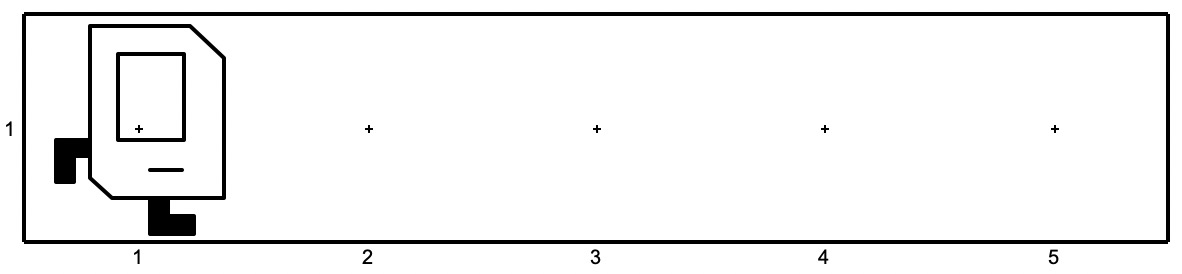
\includegraphics[scale=0.15]{images/ch04/mrofb/before.jpg}}
\caption{}
\label{fig:mrofb_recur1}
\end{figure}

ဖန်ရှင် စတင် လုပ်ဆောင်ပါမယ်။  ရှေ့မှာရှင်းနေတဲ့ အတွက် \fCode{if} ဘလောက်ကို လုပ်မှာပါ
%
\setlength{\fboxsep}{0pt}
\begin{minted}[frame=\mintframe, framerule=\mintrule,framesep= \mintsep, xleftmargin=\xlftmargin
    , bgcolor=mintbgcolor,rulecolor=mintrulecolor
    , python3=true,escapeinside=ßß]{python}
put_beeper()
move()
make_beeper_row() # ß\fEn{recursive call}ß
\end{minted}
%
ဘိပါချ၊ ရှေ့တိုး $\big\llbracket$ပုံ (\fRefNo{\ref{fig:mrofb_recur}}) (\fRefNo{\subref{fig:mrofb_recur2}})  ကြည့်ပါ$\big\rrbracket$ ပြီးရင် သူ့ကိုယ်သူ  ပြန်ခေါ်ထားတယ်။ ဒါဟာ ပထမဆုံး တစ်ကြိမ်ပါ။ ဖန်ရှင်ခေါ်ရင် ဖြစ်မြဲအတိုင်းပဲ ဖန်ရှင်နဲ့ သက်ဆိုင်တဲ့ ဘလောက်ကို ဆောက်ရွက်တာပေါ့။ ဒီတော့ \fCode{make\_beeper\_row} ဖန်ရှင်ဘလောက်ကိုပဲ တစ်ခါထပ်လုပ်မှာပါ။ ရှေ့မှာ ရှင်းနေတဲ့အတွက် \fCode{if} အပိုင်းကို လုပ်တယ်
%
\setlength{\fboxsep}{0pt}
\begin{minted}[frame=\mintframe, framerule=\mintrule,framesep= \mintsep, xleftmargin=\xlftmargin
    , bgcolor=mintbgcolor,rulecolor=mintrulecolor
    , python3=true,escapeinside=ßß]{python}
put_beeper()
move()
make_beeper_row() # ß\fEn{recursive call}ß
\end{minted}
%
ဘိပါချ၊ ရှေ့တိုး $\big\llbracket$ပုံ (\fRefNo{\ref{fig:mrofb_recur}}) (\fRefNo{\subref{fig:mrofb_recur3}})$\big\rrbracket$ ပြီး သူ့ကိုယ်သူ ပြန်ခေါ်ထားတဲ့ကိစ္စ တစ်ခါထပ်ဖြစ်ပြန်တယ်။ ဒါနဲ့ဆို နှစ်ကြိမ်။ ဖန်ရှင်ဘလောက် အလုပ် ပြန်လုပ်မယ်။ ရှေ့မှာရှင်းတယ်၊ \fCode{if} ကိုပဲ ထပ်လုပ်
%
\setlength{\fboxsep}{0pt}
\begin{minted}[frame=\mintframe, framerule=\mintrule,framesep= \mintsep, xleftmargin=\xlftmargin
    , bgcolor=mintbgcolor,rulecolor=mintrulecolor
    , python3=true,escapeinside=ßß]{python}
put_beeper()
move()
make_beeper_row() # ß\fEn{recursive call}ß
\end{minted}
%
ပုံ (\fRefNo{\ref{fig:mrofb_recur}}) (\fRefNo{\subref{fig:mrofb_recur4}}) နေရာရောက်ပြီး သူ့ကိုယ်သူ ထပ်ခေါ်ထားပြန်တယ်။ သုံးကြိမ်ရှိပြီ။ ဒီတစ်ခါလည်း \fCode{if} အပိုင်းပဲ ထပ်လုပ်
%
\setlength{\fboxsep}{0pt}
\begin{minted}[frame=\mintframe, framerule=\mintrule,framesep= \mintsep, xleftmargin=\xlftmargin
    , bgcolor=mintbgcolor,rulecolor=mintrulecolor
    , python3=true,escapeinside=ßß]{python}
put_beeper()
move()
make_beeper_row() # ß\fEn{recursive call}ß
\end{minted}
%
ရှေ့တိုးပြီးရင် နံရံပိတ်နေပြီ $\big\llbracket$ပုံ (\fRefNo{\ref{fig:mrofb_recur}}) (\fRefNo{\subref{fig:mrofb_recur5}})$\big\rrbracket$။ သူ့ကိုယ်သူ ခေါ်တယ်။ ရှေ့မှာ ပိတ်နေတဲ့အတွက် \fCode{else} အပိုင်းကို လုပ်မှာပါ။
%
\setlength{\fboxsep}{0pt}
\begin{minted}[frame=\mintframe, framerule=\mintrule,framesep= \mintsep, xleftmargin=\xlftmargin
    , bgcolor=mintbgcolor,rulecolor=mintrulecolor
    , python3=true,escapeinside=ßß]{python}
put_beeper()
\end{minted}
%
သူ့ကိုယ်သူ ပြန်ခေါ်တဲ့ကစ္စ ထပ်မဖြစ်တော့ဘူး။ ဒီမှာပဲ ပြီးဆုံးသွားတယ်။ ရီကားဆစ်ဖ် ဖန်ရှင် အလုပ်လုပ်ပုံ အခြေခံသဘောတရားက ဒါပါပဲ။ \fEn{loop} တွေ မသုံးဘဲ ပြန်ကျော့နေတဲ့ သဘောကို ရီကားဆစ်ဖ်ဖန်ရှင်မှာ တွေ့ရပါတယ်။ ဖန်ရှင်က သူ့ကိုယ်သူ (သို့ ကိုယ့်ကိုကိုယ်) ပြန်ခေါ်တာကို \fEnEmp{recursive call} လို့ခေါ်ပါတယ်။ ဒက်ဖ်နေးရှင်းအရ \fEn{recursive function} တွေမှာ \fEn{recursive call} အနည်းဆုံး တစ်ခု ပါရမှာ ဖြစ်ပါတယ်။


%ဒီတိုင်း ဆက်ကြည့်သွားရင် လေးကြိမ်မြောက် ရီကားဆစ်ဖ်‌ ကောလ်မှာ ရှေ့မှာနံရံပိတ်နေပြီ $\big\llbracket$ပုံ (\fRefNo{\ref{fig:mrofb_recur}}) (\fRefNo{\subref{fig:mrofb_recur4}})$\big\rrbracket$။ ဒီတော့ \fCode{else} အပိုင်း အလုပ်လုပ်ပါမယ်။ နောက်ဆုံး ဘိပါချမယ်။ ရီကားဆစ်ဖ်ကောလ် ဆက်မဖြစ်တော့ဘူး။ ဒီအခါ တစ်ဖက်စာမျက်နှာ \fEnEmpBf{*Initial Call*} ကွန်းမန့်အောက် ကနဦး \fCode{make\_beeper\_row} ဖန်ရှင်ကောလ်ကနေ စတင်ဖြစ်ပေါ်စေတဲ့ ရီးကားဆစ်ဖ်ဖန်ရှင် လုပ်ဆောင်မှုလည်း ပြီးဆုံးသွားမှာဖြစ်တယ်။

\begin{figure}[thb!]
    \newcommand{\figpctw}{0.49}
    \begin{subfigure}[t]{{\figpctw}\textwidth}
        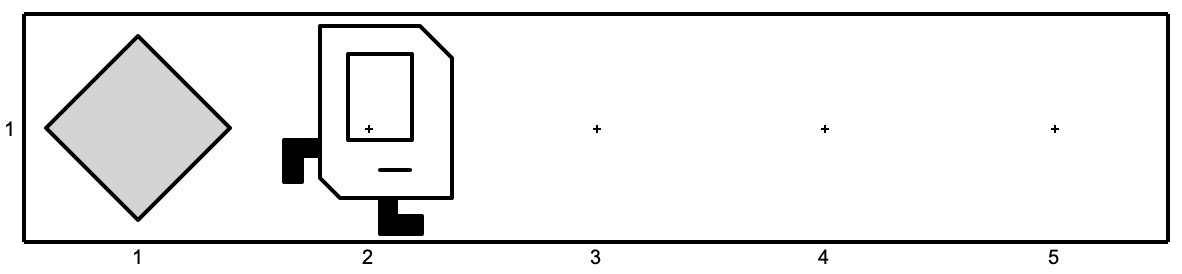
\includegraphics[scale=0.15]{images/ch04/mrofb/1st_iter.jpg}
        \caption{ပထမ တစ်ကျော့ပြီး}  
        \label{fig:mrofb_recur2}   
    \end{subfigure}
    \begin{subfigure}[t]{{\figpctw}\textwidth}
        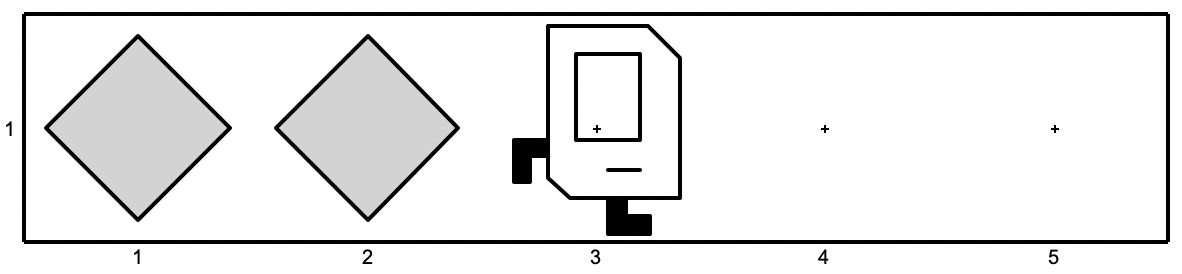
\includegraphics[scale=0.15]{images/ch04/mrofb/2nd_iter.jpg}
        \caption{ဒုတိယ တစ်ကျော့ပြီး}  
        \label{fig:mrofb_recur3}  
    \end{subfigure}
    \begin{subfigure}[t]{{\figpctw}\textwidth}
        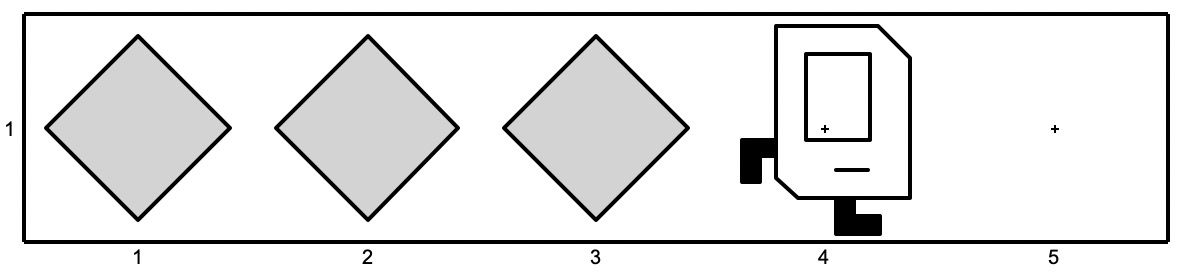
\includegraphics[scale=0.15]{images/ch04/mrofb/3rd_iter.jpg}
        \caption{တတိယ တစ်ကျော့ပြီး}  
        \label{fig:mrofb_recur4}  
    \end{subfigure}
    \begin{subfigure}[t]{{\figpctw}\textwidth}
        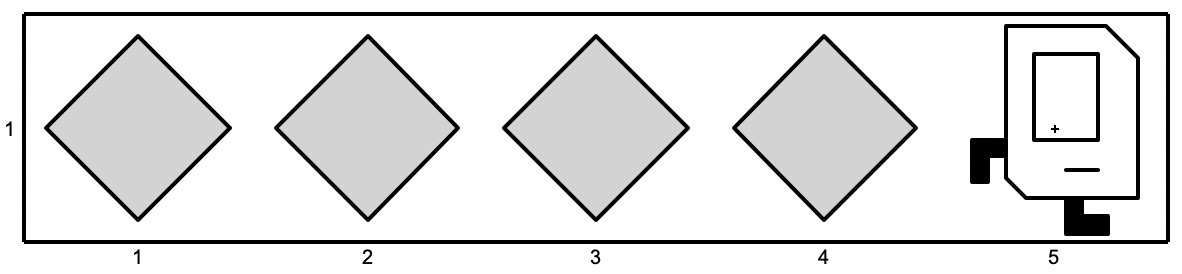
\includegraphics[scale=0.15]{images/ch04/mrofb/4th_iter.jpg}
        \caption{စတုတ္ထမြောက် ကျော့ပြီး}  
        \label{fig:mrofb_recur5}  
    \end{subfigure}
    \begin{subfigure}[t]{{\figpctw}\textwidth}
        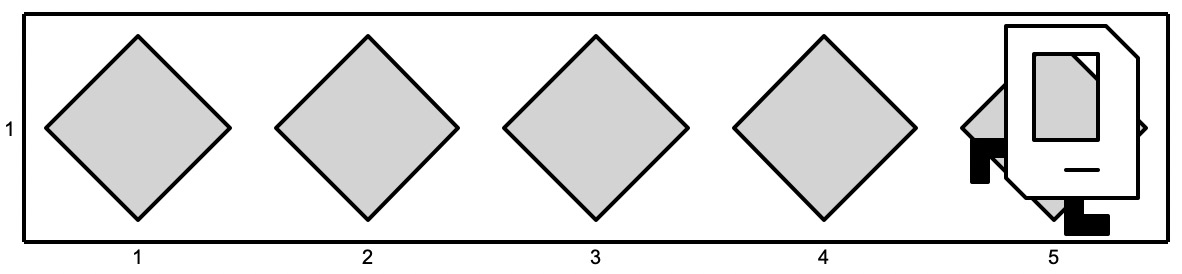
\includegraphics[scale=0.15]{images/ch04/mrofb/after.jpg}
        \caption{နောက်ဆုံး \fCptCodeBf{putBeeper} လုပ်ပြီး}    
        \label{fig:mrofb_recur6}
    \end{subfigure}
    \caption{}
    \label{fig:mrofb_recur}
\end{figure}


%
\setlength{\fboxsep}{0pt}
\begin{minted}[frame=\mintframe, framerule=\mintrule,framesep= \mintsep, xleftmargin=\xlftmargin
    , bgcolor=mintbgcolor,rulecolor=mintrulecolor
    , python3=true,escapeinside=ßß]{python}
def make_beeper_row():
    if front_is_clear():ß\tikzmark{a2}ß
        put_beeper()
        move()
        make_beeper_row()ß\tikzmark{a3}ß
    else:
        put_beeper()ß\tikzmark{a4}ß

make_beeper_row()ß\tikzmark{a1}ß
\end{minted}
%
\begin{tikzpicture}[
  remember picture,
  overlay,
  annotation/.style={
    inner sep=0pt,
    outer sep=0pt,
    outer xsep=0mm,
    fill=yellow!80!black,
    text width=5cm
  },
  >={Stealth[inset=0pt, angle=30:7pt]}
]
\draw[->, thick] ([yshift=0ex] pic cs:a1) -- ++(3,0) |- ([yshift=1.4ex]pic cs:a2);%
\draw[->, thin,blue] ([yshift=0ex] pic cs:a3) -- ++(1,0) |- ([yshift=0.5ex] pic cs:a2);%
\draw[->, thin,blue] ([yshift=1.2ex] pic cs:a3) -- ++(.7,0) |- ([yshift=-.4ex] pic cs:a2);%
\draw[->, thin,red] ([yshift=0.5ex] pic cs:a4) -- ++(.7,0) |- ([yshift=1.2ex] pic cs:a1);%
\end{tikzpicture}%
\btwntikzannoandpar

ရီကားဆစ်ဖ်ကောလ် ဖြစ်တာကို စိတ်ကူးပုံဖော်ကြည့်ဖို့ ပြထားတာပါ။ အပြင်ဆုံး မြှားအနက်က ကန\allowbreak ဦး ဖန်ရှင်ကောလ် စတင်တာဖြစ်‌ပေါ်တာကို ဖော်ပြတယ်။ ရီကားဆစ်ဖ်ကောလ် မဟုတ်သေးဘူး။ မြှားအပြာက ရီကားဆစ်ဖ်ကောလ်ကြောင့် ဖန်ရှင်အစ ပြန်ရောက်သွားတာကို ပြတယ်။ ပထမနဲ့ ဒုတိယ ရီကားဆစ်ဖ်ကောလ် နှစ်ခုအတွက်ပြထားတာပါ။ ရှေ့က ဥပမာအတွက် မြှားအပြာ လေးခု ရှိရမှာပါ (ရီကားဆစ်ဖ်ကောလ် လေးကြိမ်အတွက်)။  မြှားအပြာ နောက်ထပ် နှစ်ခုရှိတယ် မှတ်ယူပါ (ပုံမှာထပ်ထည့်ရင် ကြပ်ညပ်ပြီး ကြည့်ရရှုပ်လို့ မဆွဲပြတာ)။ လေးကြိမ်မြောက်မှာ ရီကားဆစ်ဖ်ကောလ် ထပ်မဖြစ်တော့ဘူး (\fCode{if} အပိုင်းကို မလုပ်တော့တဲ့အတွက်)။ ဘိပါချပြီး ဖန်ရှင်ကောလ် စခဲ့တဲ့နေရာကို ပြန်ရောက် သွားမယ် (မြှားအနီ)။ ဘယ်လို ပြန်ရောက်သွားတာလဲ ဆက်ကြည့်ရအောင်။

\subsection*{နောက်ဆုံး ရီကားဆစ်ဖ်ကောလ်မှ ပြန်လာခြင်း}
နောက်ဆုံး ရီကားဆစ်ဖ်ကောလ်ကနေ မူလ ဖန်ရှင်ခေါ်ခဲ့တဲ့ နေရာကို ဘယ်လိုပြန်ရောက်သွားတာလဲ။ ဒီကိစ္စနားလည်ဖို့ ဖန်ရှင် \fEnEmp{return} ပြန်ခြင်းအကြောင်း အရင်ကြည့်ရပါမယ်။ ဖန်ရှင်ကောလ် လုပ်ဆောင်တဲ့အခါ အဲဒီဖန်ရှင်နဲ့ သက်ဆိုင်တဲ့ ဘလောက်ဆီကို ခုန်ကျော် ရောက်ရှိသွားမှာပါ။ ဖန်ရှင်ဘလောက်ကို လုပ်ဆောင်ပြီး ခေါ်ခဲ့တဲ့ နေရာကို ပြန်လည်ရောက်ရှိသွားမှာ ဖြစ်တယ်။ ဒီဖြစ်စဉ်ကို ဖန်ရှင် \fEn{return} ပြန်တယ်လို့ ပြောပါတယ်။
%
\setlength{\fboxsep}{0pt}
\begin{minted}[frame=\mintframe, framerule=\mintrule,framesep= \mintsep, xleftmargin=\xlftmargin
    , bgcolor=mintbgcolor,rulecolor=mintrulecolor
    , python3=true,escapeinside=ßß]{python}
def main():
    turn_right()ß\tikzmark{b1}ß
    move()
    turn_right()
    move()

def turn_right():
    turn_left()ß\tikzmark{b2}ß
    turn_left()
    turn_left()ß\tikzmark{b3}ß
\end{minted}
\begin{tikzpicture}[
  remember picture,
  overlay,
  annotation/.style={
    inner sep=0pt,
    outer sep=0pt,
    outer xsep=1mm,
    fill=yellow!80!black,
    text width=5cm
  },
  >={Stealth[inset=0pt, angle=30:7pt]}
]
\draw[->, thin] (pic cs:b1)  ++(0,1.2ex) -- ++(1,0) |- ([yshift=0.5ex] pic cs:b2);
\draw[->, thin, red] (pic cs:b3)  ++(0,.5ex) -- ++(2,0) |- (pic cs:b1);
\end{tikzpicture}%
ပထမ \fCode{turn\_right} ကောလ် လုပ်ဆောင်တဲ့အခါ ကောလ်လုပ်တဲ့ နေရာကနေ \fCode{turn\_right} ဖန်ရှင်ထဲကို \fEn{jump} လုပ်ပြီး ရောက်သွားတယ်။ မြှားအနက်နဲ့ ပြထားတယ်။ ဖန်ရှင်ဘလောက် လုပ်ဆောင်ပြီးတဲ့အခါ ခေါ်ခဲ့တဲ့နေရာ \fCode{main} ဖန်ရှင်ထဲ ပြန်ရောက်သွားတယ် (မြှားအနီ)။ ဒုတိယ \fCode{turn\_right} လည်း ထိုနည်းတူစွာပဲ ဖြစ်ပါတယ်။


%
\setlength{\fboxsep}{0pt}
\begin{minted}[frame=\mintframe, framerule=\mintrule,framesep= \mintsep, xleftmargin=\xlftmargin
    , bgcolor=mintbgcolor,rulecolor=mintrulecolor
    , python3=true,escapeinside=ßß]{python}
def main():
    turn_right()
    move()
    turn_right()ß\tikzmark{c1}ß
    move()

def turn_right():
    turn_left()ß\tikzmark{c2}ß
    turn_left()
    turn_left()ß\tikzmark{c3}ß
\end{minted}
\begin{tikzpicture}[
  remember picture,
  overlay,
  annotation/.style={
    inner sep=0pt,
    outer sep=0pt,
    outer xsep=1mm,
    fill=yellow!80!black,
    text width=5cm
  },
  >={Stealth[inset=0pt, angle=30:7pt]}
]
\draw[->, thin] (pic cs:c1)  ++(0,1.2ex) -- ++(1,0) |- ([yshift=0.5ex] pic cs:c2);
\draw[->, thin, red] (pic cs:c3)  ++(0,.5ex) -- ++(2,0) |- (pic cs:c1);
\end{tikzpicture}
\btwntikzannoandpar

နှစ်ဆင့်၊ သုံးဆင့် ဖန်ရှင်ကောလ်တွေမှာလည်း ဒီသဘောတရား အတိုင်းပါပဲ။ အောက်ဖော်ပြပါ ပရိုဂရမ်ကုဒ်ကို ကြည့်ပါ။ \fCode{main} ဖန်ရှင်ထဲကနေ \fCode{do\_tricks} ဆီကို ရောက်သွားမယ်။ \fCode{do\_tricks} ထဲကနေ \fCode{put\_two} ထဲကို ရောက်သွားမယ်။ 
%
\setlength{\fboxsep}{0pt}
\begin{minted}[frame=\mintframe, framerule=\mintrule,framesep= \mintsep, xleftmargin=\xlftmargin
    , bgcolor=mintbgcolor,rulecolor=mintrulecolor
    , python3=true,escapeinside=ßß]{python}
def main():
    do_tricks()ß\tikzmark{d1}ß
    move()

def do_tricks():
    move()ß\tikzmark{d2}ß
    put_two()ß\tikzmark{d3}ß
    turn_left()
    move()ß\tikzmark{d4}ß

def put_two():
    put_beeper()ß\tikzmark{d5}ß
    put_beeper()ß\tikzmark{d6}ß
\end{minted}
\begin{tikzpicture}[
  remember picture,
  overlay,
  annotation/.style={
    inner sep=0pt,
    outer sep=0pt,
    outer xsep=1mm,
    fill=yellow!80!black,
    text width=5cm
  },
  >={Stealth[inset=0pt, angle=30:7pt]}
]
\draw[->, thin] (pic cs:d1)  ++(0,1.2ex) -- ++(1,0) |- ([yshift=0.5ex] pic cs:d2);
\draw[->, thin] (pic cs:d3)  ++(0,1.2ex) -- ++(1,0) |- ([yshift=0.5ex] pic cs:d5);
\draw[->, thin, red] (pic cs:d6)  ++(0,.5ex) -- ++(0.7,0) |- (pic cs:d3);
\draw[->, thin, red] (pic cs:d4)  ++(0,.5ex) -- ++(2.1,0) |- (pic cs:d1);
\end{tikzpicture}%
%

\fCode{put\_two} ပြီးသွားတဲ့အခါ \fCode{do\_tricks} ထဲ ပြန်ရောက်သွားမယ်။ \fCode{turn\_left}\fEn{,} \fCode{move} ဆက်လုပ်ပြီး \fCode{do\_tricks} ခေါ်ခဲ့တဲ့နေရာ \fCode{main} ထဲ ပြန်ရောက်သွားမယ်။ နောက်ဆုံး \fCode{main} ထဲက \fCode{move}  ကို ဆက်လုပ်ပါတယ်။

ဖန်ရှင် အဆင့်ဆင့် ခေါ်ထားတဲ့အခါ နောက်ဆုံးခေါ်တဲ့ ဖန်ရှင်က အရင်ဆုံး \fEn{return} ပြန်ပါတယ်။ \fCode{main} ကနေ \fCode{do\_tricks} ကိုခေါ်၊ \fCode{do\_tricks} ကနေ \fCode{put\_two} ကိုခေါ်ထားရင် \fCode{put\_two} ကနေ \fCode{do\_tricks} ဆီကို အရင် \fEn{return} ပြန်တယ်။ ပြီးတော့မှ \fCode{do\_tricks} ကနေ \fCode{main} ကို ပြန်ရောက်မှာပါ။ ဒီသဘောအရ \fCode{put\_two} \fEn{return} မပြန်မချင်း \fCode{do\_tricks} ဖန်ရှင်မပြီးသေးဘူး။ \fCode{put\_two} ကနေပြန်လာပြီးမှ ကျန်တဲ့ \fCode{turn\_left}\fEn{,} \fCode{move} ဆက်လုပ်တယ်။ ပြီးတော့မှ \fCode{do\_tricks} ဖန်ရှင်က \fEn{return} ပြန်ပါတယ်။ 


ရီကားဆစ်ဖ် ဖန်ရှင်ကောလ်တွေ ဘယ်လို \fEn{return} ပြန်လဲ။ ရှေ့ကလို မြှားတွေနဲ့ ဆွဲပြလို့ ရပေမဲ့ ကြည့်ရတာ ရှုပ်ရှက်ခတ်နေမှာပါ။ အခုလို မြင်ကြည့်ရင် ပိုရှင်းပါတယ်။
%
\setlength{\fboxsep}{0pt}
\begin{minted}[frame=\mintframe, framerule=\mintrule,framesep= \mintsep, xleftmargin=\xlftmargin
    , bgcolor=mintbgcolor,rulecolor=mintrulecolor
    , python3=true,escapeinside=ßß]{python}
# ß\fEn{initial call}ß
make_beeper_row()ß\tikzmarknode{e1}ß
    # ß\fEn{1\textsuperscript{\fEn{st}} recur}ß
    make_beeper_row()ß\tikzmarknode{e2}ß
        # ß\fEn{2\textsuperscript{\fEn{nd}} recur}ß
        make_beeper_row()ß\tikzmarknode{e3}ß
            # ß\fEn{3\textsuperscript{\fEn{rd}} recur}ß
            make_beeper_row()ß\tikzmarknode{e4}ß
                # ß\fEn{4\textsuperscript{\fEn{th}} recur}ß
                make_beeper_row()ß\tikzmarknode{e5}ß
\end{minted}
\begin{tikzpicture}[
  remember picture,
  overlay,
  annotation/.style={
    inner sep=0pt,
    outer sep=0pt,
    outer xsep=1mm,
    fill=yellow!80!black,
    text width=5cm
  },
  >={Stealth[inset=0pt, angle=30:7pt]}
]
\draw[->, thin] (pic cs:e1)  ++(0,.3ex) .. controls ([xshift=1.1cm,yshift=-.11cm]pic cs:e1) and ([xshift=.5cm,yshift=.5cm]pic cs:e2) ..  ([yshift=1.2ex] pic cs:e2);
\draw[->, thin] (pic cs:e2)  ++(0,0ex) .. controls ([xshift=1.1cm,yshift=-.11cm]pic cs:e2) and ([xshift=.5cm,yshift=.5cm]pic cs:e3) ..  ([yshift=1.2ex] pic cs:e3);
\draw[->, thin] (pic cs:e3)  ++(0,0ex) .. controls ([xshift=1.1cm,yshift=-.11cm]pic cs:e3) and ([xshift=.5cm,yshift=.5cm]pic cs:e4) ..  ([yshift=1.2ex] pic cs:e4);
\draw[->, thin] (pic cs:e4)  ++(0,0ex) .. controls ([xshift=1.1cm,yshift=-.11cm]pic cs:e4) and ([xshift=.5cm,yshift=.5cm]pic cs:e5) ..  ([yshift=.7ex] pic cs:e5);
\draw[->, thin, red] (pic cs:e5)  ++(0,0ex) .. controls ([xshift=1.7cm,yshift=.4cm]pic cs:e5) and ([xshift=1cm,yshift=.2cm]pic cs:e4) ..  ([yshift=.5ex] pic cs:e4);
\draw[->, thin, red] (pic cs:e4)  ++(0,1ex) .. controls ([xshift=1.7cm,yshift=.4cm]pic cs:e4) and ([xshift=1cm,yshift=.2cm]pic cs:e3) ..  ([yshift=.5ex] pic cs:e3);
\draw[->, thin, red] (pic cs:e3)  ++(0,1ex) .. controls ([xshift=1.7cm,yshift=.4cm]pic cs:e3) and ([xshift=1cm,yshift=.2cm]pic cs:e2) ..  ([yshift=.5ex] pic cs:e2);
\draw[->, thin, red] (pic cs:e2)  ++(0,1ex) .. controls ([xshift=1.7cm,yshift=.4cm]pic cs:e2) and ([xshift=1cm,yshift=.2cm]pic cs:e1) ..  ([yshift=.7ex] pic cs:e1);
%([yshift=0.1em]a.north) to[bend left] ([yshift=0.1em]b.north);}
\end{tikzpicture}%
\btwntikzannoandpar

မြှားအနက်တွေက ဖန်ရှင်ကောလ်  တစ်ဆင့်ပြီးတစ်ဆင့် ဖြစ်တာကို ပြတာပါ။ အထက်မှအောက် အစီ\allowbreak အစဉ်အတိုင်း ဖြစ်ပါတယ်။ ‌လေးကြိမ်မြောက်မှာ နောက်ထပ် ရီကားဆစ်ဖ်ကောလ် ထပ်မဖြစ်တော့ဘဲ နောက်ဆုံး ရီကားဆစ်ဖ်ကောလ်က အရင်ဆုံး \fEn{return} စပြန်ပါတယ် (အောက်ဆုံး မြှားအနီနဲ့ ပြထား)။ ဒီအခါ တတိယ ရီကားဆစ်ဖ်ကောလ်ကို ပြန်ရောက်သွားမှာပါ။ ဒီအတိုင်း တစ်ဆင့်ပြီးတစ်ဆင့် အထက်ကို \fEn{return} ပြန်ပြီး နောက်ဆုံးမှာ ပထမဆုံး ခေါ်ခဲ့တဲ့နေရာ ပြန်ရောက်သွားမှာပါ။ (အခုပြထားတာကို တကယ့် \fEn{Python} ကုဒ် အနေနဲ့ မယူဆရပါ၊ ဖြစ်စဉ် နားလည်အောင် ပြခြင်းသာဖြစ်ပါတယ်)။ နဲနဲပြင်ထားတဲ့ \fCode{make\_beeper\_\allowbreak row}  ဗားရှင်းမှာ \fEn{return} ပြန်တဲ့ ဖြစ်စဉ်ကို ကြည့်ရအောင်။ 

%
\setlength{\fboxsep}{0pt}
\begin{minted}[frame=\mintframe, framerule=\mintrule,framesep= \mintsep, xleftmargin=\xlftmargin
    , bgcolor=mintbgcolor,rulecolor=mintrulecolor
    , python3=true,escapeinside=ßß]{python}
make_beeper_row()
\end{minted}
%
\betweenminted{\medskipamount}
%
\setlength{\fboxsep}{0pt}
\begin{minted}[frame=\mintframe, framerule=\mintrule,framesep= \mintsep, xleftmargin=\xlftmargin
    , bgcolor=mintbgcolor,rulecolor=mintrulecolor
    , python3=true,escapeinside=ßß]{python}
def make_beeper_row():
    if front_is_clear():
        put_beeper()
        move()
        make_beeper_row()
        turn_left()
        move()
    else:
        put_beeper()
\end{minted}
%
\btwntikzannoandpar

\fCode{if}  အပိုင်း ရီကားဆစ်ဖ်ကောလ်ပြီး  \fCode{turn\_\allowbreak left} နဲ့ \fCode{move} ထပ်ဖြည့်ထားတာ။  ရီကားဆစ်ဖ်ကောလ် \fEn{return} ပြန်လာပြီးမှ ဒီနှစ်ခု ဆက်လုပ်မှာပါ။  နောက်ဆုံး ရီကားဆစ်ဖ်ကောလ်က \fEn{return} စဖြစ်တယ်။ ဒီတော့မှ တတိယအောက် \fCode{turn\_\allowbreak left} နဲ့ \fCode{move} ကို လုပ်ဆောင်မှာပါ။ ပြီးမှ တတိယကောလ် \fEn{return} ပြန်တယ်။ ဒီအတိုင်း အထက်ကို တက်သွားပြီး ကျန်နေသေးတဲ့ စတိတ်မန့်တွေကို လုပ်ဆောင်ပါတယ်။ ပထမဆုံးကောလ်အောက် ကျန်နေတာတွေ နောက်ဆုံးကျမှ ပြီးမှာပါ။

%
\setlength{\fboxsep}{0pt}
\begin{minted}[frame=\mintframe, framerule=\mintrule,framesep= \mintsep, xleftmargin=\xlftmargin
    , bgcolor=mintbgcolor,rulecolor=mintrulecolor
    , python3=true,escapeinside=ßß]{python}
# ß\fEn{initial call}ß
make_beeper_row()ß\tikzmarknode{f1}ß
    # ß\fEn{1\textsuperscript{\fEn{st}} recur}ß
    make_beeper_row()ß\tikzmarknode{f2}ß
    turn_left()
    move()ß\tikzmarknode{f2a}ß
        # ß\fEn{2\textsuperscript{\fEn{nd}} recur}ß
        make_beeper_row()ß\tikzmarknode{f3}ß
        turn_left()
        move()ß\tikzmarknode{f3a}ß
            # ß\fEn{3\textsuperscript{\fEn{rd}} recur}ß
            make_beeper_row()ß\tikzmarknode{f4}ß
            turn_left()
            move()ß\tikzmarknode{f4a}ß
                # ß\fEn{4\textsuperscript{\fEn{th}} recur}ß
                make_beeper_row()ß\tikzmarknode{f5}ß
\end{minted}
\begin{tikzpicture}[
  remember picture,
  overlay,
  annotation/.style={
    inner sep=0pt,
    outer sep=0pt,
    outer xsep=1mm,
    fill=yellow!80!black,
    text width=5cm
  },
  >={Stealth[inset=0pt, angle=30:7pt]}
]
\draw[->, thin] (pic cs:f1)  ++(0,.3ex) .. controls ([xshift=1.1cm,yshift=-.11cm]pic cs:f1) and ([xshift=.5cm,yshift=.5cm]pic cs:f2) ..  ([yshift=1.2ex] pic cs:f2);
\draw[->, thin] (pic cs:f2)  ++(0,0ex) .. controls ([xshift=1.1cm,yshift=-.11cm]pic cs:f2) and ([xshift=.5cm,yshift=.5cm]pic cs:f3) ..  ([yshift=1.2ex] pic cs:f3);
\draw[->, thin] (pic cs:f3)  ++(0,0ex) .. controls ([xshift=1.1cm,yshift=-.11cm]pic cs:f3) and ([xshift=.5cm,yshift=.5cm]pic cs:f4) ..  ([yshift=1.2ex] pic cs:f4);
\draw[->, thin] (pic cs:f4)  ++(0,0ex) .. controls ([xshift=1.1cm,yshift=-.11cm]pic cs:f4) and ([xshift=.5cm,yshift=.5cm]pic cs:f5) ..  ([yshift=.7ex] pic cs:f5);
\draw[->, thin, red] (pic cs:f5)  ++(0,0ex) .. controls ([xshift=1.7cm,yshift=.4cm]pic cs:f5) and ([xshift=1cm,yshift=.2cm]pic cs:f4) ..  ([yshift=.5ex] pic cs:f4);
\draw[->, thin, red] (pic cs:f4a)  ++(0,.5ex) .. controls ([xshift=4.5cm,yshift=.7cm]pic cs:f4a) and ([xshift=1cm,yshift=.2cm]pic cs:f3) ..  ([yshift=.5ex] pic cs:f3);
\draw[->, thin, red] (pic cs:f3a)  ++(0,.5ex) .. controls ([xshift=4.5cm,yshift=.7cm]pic cs:f3a) and ([xshift=1cm,yshift=.2cm]pic cs:f2) ..  ([yshift=.5ex] pic cs:f2);
\draw[->, thin, red] (pic cs:f2a)  ++(0,.5ex) .. controls ([xshift=4.5cm,yshift=.7cm]pic cs:f2a) and ([xshift=1cm,yshift=.2cm]pic cs:f1) ..  ([yshift=.5ex] pic cs:f1);
%([yshift=0.1em]a.north) to[bend left] ([yshift=0.1em]b.north);}
\end{tikzpicture}


ရီကားဆစ်ဖ်ကောလ် နှစ်ခါပဲ ဖြစ်မယ်ဆိုရင် အောက်ပါအတိုင်း မြင်ကြည့်လို့ ရပါတယ်။ မြှားအပြာနှစ်ခုက ရီကားဆစ်ဖ်ကောလ်ဖြစ်တာ။ ဒုတိယကောလ်က ဘိပါချပြီး (\fCode{else} အပိုင်း) အရင် \fEn{return} မယ်။ အထက်ကို ညွှန်တဲ့ မြှားအနီကို ကြည့်ပါ။ ဘယ်လှည့်၊ ရှေ့တိုးပြီး ပထမ ကောလ်က နောက်မှ \fEn{initial call} လုပ်ခဲ့တဲ့ဆီ ပြန်ရောက်တာ။ အောက်ကိုညွှန်တဲ့ မြှားအနီကို ကြည့်ပါ။
%
\setlength{\fboxsep}{0pt}
\begin{minted}[frame=\mintframe, framerule=\mintrule,framesep= \mintsep, xleftmargin=\xlftmargin
    , bgcolor=mintbgcolor,rulecolor=mintrulecolor
    , python3=true,escapeinside=ßß]{python}
def make_beeper_row():
    if front_is_clear():ß\tikzmark{g2}ß
        put_beeper()
        move()
        make_beeper_row()ß\tikzmark{g3}ß
        turn_left()
        move()ß\tikzmark{g3a}ß
    else:
        put_beeper()ß\tikzmark{g4}ß

# ß\fEn{initial call}ß
make_beeper_row()ß\tikzmark{g1}ß
\end{minted}
%
\begin{tikzpicture}[
  remember picture,
  overlay,
  annotation/.style={
    inner sep=0pt,
    outer sep=0pt,
    outer xsep=0mm,
    fill=yellow!80!black,
    text width=5cm
  },
  >={Stealth[inset=0pt, angle=30:7pt]}
]
\draw[->, thick] ([yshift=1.2ex] pic cs:g1) -- ++(3,0) |- ([yshift=1.4ex]pic cs:g2);%
\draw[->, thin,blue] ([yshift=.5ex] pic cs:g3) -- ++(1,0) |- ([yshift=0.5ex] pic cs:g2);%
\draw[->, thin,blue] ([yshift=1.4ex] pic cs:g3) -- ++(.7,0) |- ([yshift=-.4ex] pic cs:g2);%
\draw[->, thin,red] ([yshift=0.5ex] pic cs:g4) -- ++(1.5,0) |- ([yshift=-.4ex] pic cs:g3);%
\draw[->, thin,red] ([yshift=0.5ex] pic cs:g3a) -- ++(1.5,0) |- ([yshift=0ex] pic cs:g1);%
\end{tikzpicture}%
\btwntikzannoandpar

ရီကားဆစ်ဖ် ဖန်ရှင်အကြောင်း လေ့လာတဲ့အခါ ဘီဂင်နာအများစု ကြေကြေညက်ညက် နားလည်ဖို့အတွက် အခက်အခဲဆုံးတစ်ခုက \fEn{return} ပြန်တဲ့ သဘောတရားပါပဲ။  များများစဉ်းစား၊ များများလေ့ကျင့်ရင် ဒီအခက်အခဲ ကျော်ဖြတ်နိုင်မှာပါ။ \fCode{if...else} အပြီးမှာ \fCode{put\_beeper} လေးတစ်ခုပဲ ထပ်ဖြည့်လိုက်ရင် ဘယ်လိုဖြစ်မလဲ။
%
\setlength{\fboxsep}{0pt}
\begin{minted}[frame=\mintframe, framerule=\mintrule,framesep= \mintsep, xleftmargin=\xlftmargin
    , bgcolor=mintbgcolor,rulecolor=mintrulecolor
    , python3=true,escapeinside=ßß]{python}
# File: make_beeper_row2.py
def make_beeper_row():
    if front_is_clear():
        put_beeper()
        move()
        make_beeper_row()
        turn_left()
        move()
    else:
        put_beeper()
    put_beeper()

# ß\fEn{initial call}ß
make_beeper_row()
\end{minted}
ပုံ (\fRefNo{\ref{fig:mrofb2}}) (\fRefNo{\subref{fig:mrofb2_1}}) နဲ့ (\fRefNo{\subref{fig:mrofb2_2}}) က မတိုင်မီနဲ့ ပြီးနောက် အခြေအနေပါ။ နောက်ဆုံးမှာ ဘိပါလေးခုကို ပါတ်လည် ဘယ်လိုချသွားလဲ စဉ်းစားကြည့်ပါ။ ရှေ့မှာဖော်ပြခဲ့သလို ဖန်ရှင်ကောလ်တွေ တစ်ဆင့်ပြီးတစ်ဆင့် ဖြစ်ပုံနဲ့ \fEn{return} ဖြစ်ပုံကို မြှားဆွဲကြည့်ပါ။
\begin{figure}[thb!]
    \newcommand{\figpctw}{0.49}
    \begin{subfigure}[t]{{\figpctw}\textwidth}
        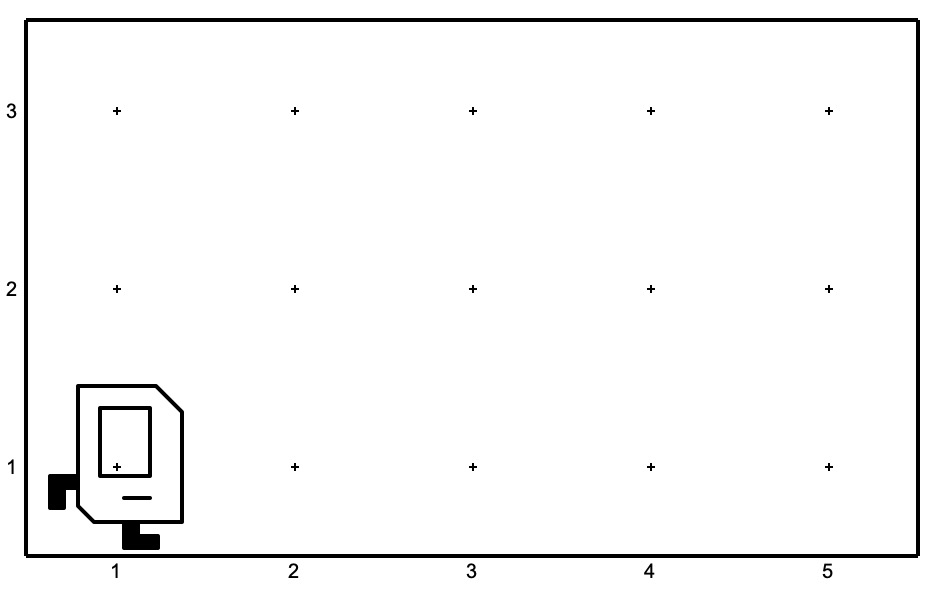
\includegraphics[scale=0.19]{images/ch04/mrofb2/1.jpg}
        \caption{}  
        \label{fig:mrofb2_1}   
    \end{subfigure}
    \begin{subfigure}[t]{{\figpctw}\textwidth}
        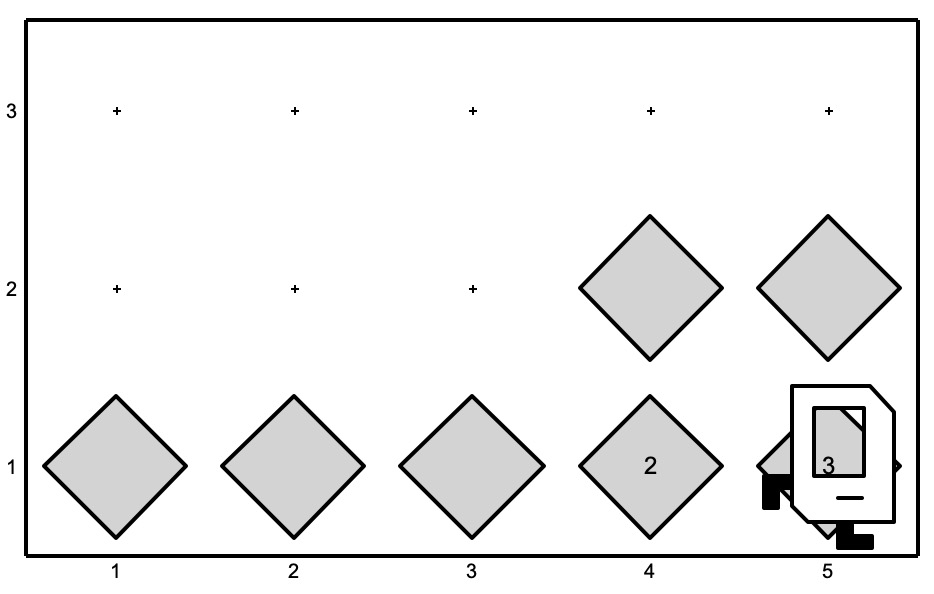
\includegraphics[scale=0.19]{images/ch04/mrofb2/2.jpg}
        \caption{}  
        \label{fig:mrofb2_2}  
    \end{subfigure}
    \caption{}
    \label{fig:mrofb2}
\end{figure}

\section{ရီကားဆစ်ဖ်နည်းဖြင့် ပုစ္ဆာဖြေရှင်းခြင်း}
ရှေ့ စက်ရှင်မှာ လေ့လာခဲ့တာက ရီကားဆစ်ဖ်ဖန်ရှင် ဘယ်လို အလုပ်လုပ်လဲပဲ ရှိပါသေးတယ်။ တစ်နည်း\allowbreak အားဖြင့် မက္ကနစ်ဇမ် \fEn{(mechanism)} ကို လေ့လာတာပါ။ အခုတစ်ခါ ရီကားဆစ်ဖ်ဖန်ရှင်တွေနဲ့ ပုစ္ဆာတွေ ဘယ်လိုဖြေရှင်းမလဲ ဆက်လက်လေ့လာပါမယ်။  ‘ရီကားဆစ်ဖ် စဉ်းစားခြင်း’ \fEn{(thinking recursively}\fEn{)} သို့မဟုတ် ‘ရီကားဆစ်ဖ်နည်းဖြင့် ပုစ္ဆာဖြေရှင်းခြင်း’ \fEn{(solving problems recursively)} ကို လေ့လာမှာပါ။
\subsection*{ရီကားဆစ်ဖ် စဉ်းစားခြင်း ဥပမာ (၁)}
ကွန်နာမှာရှိတဲ့ ဘိပါတွေအားလုံး ကောက်မယ်ဆိုပါစို့။ ဘိပါတစ်ခုနဲ့ အထက်ရှိနိုင်တယ်။ ဘိပါမရှိတာလည်း ဖြစ်နိုင်တယ် ယူဆပါ။ ဒီအတွက် ရီကားဆစ်ဖ်ဖန်ရှင် သတ်မှတ်ပါမယ်။ 
%
\setlength{\fboxsep}{0pt}
\begin{minted}[frame=\mintframe, framerule=\mintrule,framesep= \mintsep, xleftmargin=\xlftmargin
    , bgcolor=mintbgcolor,rulecolor=mintrulecolor
    , python3=true,escapeinside=ßß]{python}
def pick_all_beepers():
    ... # ß\fEn{to do soon}ß
\end{minted}
%

ဖြေရှင်းမဲ့ကိစ္စတစ်ခုကို ၎င်းကိုယ်တိုင်နဲ့ ပုံပန်းသဏ္ဌာန်တူပြီး အရွယ်အစားအားဖြင့် တစ်ဆင့်ထက်တစ်ဆင့် သေးငယ်တဲ့ ကိစ္စတွေအဖြစ် ခွဲခြမ်းကြည့်ပါတယ်။ ဥပမာ ဘိပါငါးခုရှိတဲ့ ကိစ္စကို ဘိပါလေးခု၊ သုံးခု၊ နှစ်ခု နဲ့ တစ်ခု ရှိတဲ့ ကိစ္စတွေအဖြစ် ခွဲပြီး မြင်ကြည့်ရမှာပါ။ ဒီကိစ္စမှာ ဘိပါအရေအတွက်ဟာ အရွယ်အစားပဲ။ လေးခုရှိတဲ့ ကိစ္စဟာ ငါးခုရှိတဲ့ကိစ္စထက် အရွယ်အားဖြင့် တစ်ဆင့်ငယ်တာပေါ့။ ဘိပါမရှိတာလည်း ဖြစ်နိုင်တော့ သုညဘိပါဟာ အငယ်ဆုံးဖြစ်တယ်လို့ ယူဆနိုင်တယ်။

\fCode{pick\_all\_beepers} ဖန်ရှင်ဟာ လက်ရှိဖြေရှင်းမဲ့ အရွယ်အစားထက် တစ်ဆင့်ငယ်တဲ့ ကိစ္စကို ဖြေရှင်းနိုင်ပြီးသားလို့ မှတ်ယူရပါမယ်။ လက်ရှိဖြေရှင်းမဲ့ ကိစ္စက ဘိပါငါးခု ကောက်ရမယ်ဆိုရင် ဘိပါလေးခု ကောက်နိုင်ပြီးသားလို့ ယူဆရမှာပါ။ $n$ ဘိပါရှိတယ် ဆိုရင် $n - 1$ ဘိပါကို ကောက်နိုင်ပြီးသား ယူဆရမယ်။ \fEn{Top-down} နည်းမှာလည်း ဒီလိုပဲ မရှိသေးဘဲ၊ မလုပ်နိုင်သေးဘဲ ရှိတယ်၊ လုပ်နိုင်တယ် မှတ်ယူပြီး စဉ်းစားဖြေရှင်းတာကို ပြန်အမှတ်ရမှာပါ။ ရီကားဆစ်ဖ် စဉ်းစားတဲ့အခါမှာ လက်ရှိသတ်မှတ်နေတဲ့ ဖန်ရှင်ကိုယ်တိုင်ကို ရှိပြီးဖြစ်တယ်လို့ သဘောထားရတာ။

ပြီးတဲ့အခါ လက်ရှိကိစ္စကနေ သူ့ထက်တစ်ဆင့်ငယ်တဲ့ ကိစ္စဖြစ်သွားအောင် ဘာလုပ်ရမလဲ စဉ်းစားရတယ်။ ဘိပါငါးခုကနေ လေးခုဖြစ်အောင် ဘိပါတစ်ခု ကောက်ရမှာပေါ့။ ယျေဘုယျပြောရင် $n$ ဘိပါရှိရင် ဆိုရင် $n - 1$ ဘိပါဖြစ်သွားအောင် ဘာလုပ်ရမလဲ စဉ်းစားတာ။

လက်ရှိဖန်ရှင်ဟာ $n - 1$ ဘိပါကို ကောက်နိုင်ပြီးသားလို့ ယူဆထားတယ်။  $n$ ဘိပါရှိရင် ဘိပါတစ်ခု ကောက်လိုက်ရင် $n - 1$ ဘိပါဖြစ်သွားမယ်။  ကျန်နေတဲ့  $n - 1$ ဘိပါကောက်ဖို့ လက်ရှိဖန်ရှင်ကိုပဲ ပြန်ခေါ်လိုက်မှာပေါ့။
%
\setlength{\fboxsep}{0pt}
\begin{minted}[frame=\mintframe, framerule=\mintrule,framesep= \mintsep, xleftmargin=\xlftmargin
    , bgcolor=mintbgcolor,rulecolor=mintrulecolor
    , python3=true,escapeinside=ßß]{python}
# ß\fEn{only partially done}ß
def pick_all_beepers():
    ...
    # ß\fEn{to pick $(n)$ beepers}ß
    pick_beeper()
    pick_all_beepers() # ß\fEn{assuming it can pick $(n - 1)$ beepers}ß
    ...
\end{minted}
%
ရီကားဆစ်ဖ် စဉ်းစားတတ်ဖို့ ဒီအဆင့်က အခရာအကျဆုံးပဲ။ တစ်ဆင့်ငယ်တဲ့ ကိစ္စ $n - 1$ ကို ဖြေရှင်းနိုင်ပြီးသားလို့ မှတ်ယူပြီး လက်ရှိကစ္စ $n$ ကို ဘယ်လို ဖြေရှင်းမလဲ စဉ်းစားသွားတာ။

ဖန်ရှင်သတ်မှတ်ချက်က မပြီးသေးပါဘူး။ အသေးငယ်ဆုံး ကိစ္စကို ချွင်းချက်အနေနဲ့ စဉ်းစားရမယ်။  အသေးငယ်ဆုံးကိစ္စက ဘိပါမရှိတာ (သုည) ဖြစ်တယ်။ ဘိပါမရှိရင် ဘာမှလုပ်စရာမလိုဘူး။ $n$ နဲ့ $n - 1$ ဘိပါအတွက် အထက်ပါအတိုင်း စဉ်းစားတဲ့အခါ $n \neq 0$ လို့ ယူဆရမှာပါ။ ဒါကြောင့် ဘိပါရှိမှပဲ လုပ်အောင် အခုလိုဖြစ်ရပါမယ်

%
\setlength{\fboxsep}{0pt}
\begin{minted}[frame=\mintframe, framerule=\mintrule,framesep= \mintsep, xleftmargin=\xlftmargin
    , bgcolor=mintbgcolor,rulecolor=mintrulecolor
    , python3=true,escapeinside=ßß]{python}
# ß\fEn{finished}ß
def pick_all_beepers():
    if beepers_present():
        pick_beeper()
        pick_all_beepers()
\end{minted}
%


\subsection*{ရီကားဆစ်ဖန်ရှင် မှန်မမှန် စစ်ဆေးခြင်း}
ရီကားဆစ်ဖန်ရှင် တက်စ် \fEn{(test)} လုပ်ရင် အသေးဆုံးကိစ္စကနေ စရတယ်။ ပြီးခဲတဲ့ ဖန်ရှင်အတွက် အသေးဆုံးက သုညပါ။ ဘိပါမရှိရင် ဖန်ရှင်က မှန်ရဲ့လား အရင်ဆုံး စစ်ကြည့်ပါမယ်။

%
\setlength{\fboxsep}{0pt}
\begin{minted}[frame=\mintframe, framerule=\mintrule,framesep= \mintsep, xleftmargin=\xlftmargin
    , bgcolor=mintbgcolor,rulecolor=mintrulecolor
    , python3=true,escapeinside=ßß]{python}
# ß\fEn{assume no beeper}ß
pick_all_beepers()
\end{minted}
%
\fCode{if} ဘလောက် မလုပ်ဆောင်ဘဲ \fEn{return} ဖြစ်သွားမှာပါ (ရီကားဆစ်ဖ်ကောလ် မဖြစ်လိုက်ဘူး)။ သုညဘိပါအတွက် ဖြစ်သင့်တဲ့အတိုင်း ဖြစ်ပါတယ်။ ဘိပါတစ်ခုပဲ ရှိရင်ရော ဘယ်လိုဖြစ်မလဲ။ ဘိပါကောက်တယ် သုညဘိပါဖြစ်သွားပြီး ရီကားဆစ်ဖ်ကောလ် ဖြစ်မယ်။ တစ်ကြိမ်ပဲ ဖြစ်မယ်။ \fCode{if} ဘလောက် အလုပ်မလုပ်ဘဲ \fEn{return} ပြန်မယ်။
%
\setlength{\fboxsep}{0pt}
\begin{minted}[frame=\mintframe, framerule=\mintrule,framesep= \mintsep, xleftmargin=\xlftmargin
    , bgcolor=mintbgcolor,rulecolor=mintrulecolor
    , python3=true,escapeinside=ßß]{python}
# ß\fEn{initial call}ß
pick_all_beepers()ß\tikzmarknode{h1}ß
    # ß\fEn{1\textsuperscript{\fEn{st}} recur}ß
    pick_all_beepers()ß\tikzmarknode{h2}ß
\end{minted}
\begin{tikzpicture}[
  remember picture,
  overlay,
  annotation/.style={
    inner sep=0pt,
    outer sep=0pt,
    outer xsep=1mm,
    fill=yellow!80!black,
    text width=5cm
  },
  >={Stealth[inset=0pt, angle=30:7pt]}
]
\draw[->, thin] (pic cs:h1)  ++(0,.3ex) .. controls ([xshift=1.1cm,yshift=-.11cm]pic cs:h1) and ([xshift=.5cm,yshift=.5cm]pic cs:h2) ..  ([yshift=1.2ex] pic cs:h2);
\draw[->, thin, red] (pic cs:h2)  ++(0,1ex) .. controls ([xshift=1.7cm,yshift=.4cm]pic cs:h2) and ([xshift=1cm,yshift=.2cm]pic cs:h1) ..  ([yshift=.7ex] pic cs:h1);
%([yshift=0.1em]a.north) to[bend left] ([yshift=0.1em]b.north);}
\end{tikzpicture}%
သုံးခုရှိရင် ရီကားဆစ်ဖ်ကောလ် နှစ်ခါဖြစ်ပြီးမှ \fEn{return} ပြန်မှာပါ။
%
\setlength{\fboxsep}{0pt}
\begin{minted}[frame=\mintframe, framerule=\mintrule,framesep= \mintsep, xleftmargin=\xlftmargin
    , bgcolor=mintbgcolor,rulecolor=mintrulecolor
    , python3=true,escapeinside=ßß]{python}
# ß\fEn{initial call}ß
pick_all_beepers()ß\tikzmarknode{i1}ß
    # ß\fEn{1\textsuperscript{\fEn{st}} recur}ß
    pick_all_beepers()ß\tikzmarknode{i2}ß
        # ß\fEn{2\textsuperscript{\fEn{nd}} recur}ß
        pick_all_beepers()ß\tikzmarknode{i3}ß
\end{minted}
\begin{tikzpicture}[
  remember picture,
  overlay,
  annotation/.style={
    inner sep=0pt,
    outer sep=0pt,
    outer xsep=1mm,
    fill=yellow!80!black,
    text width=5cm
  },
  >={Stealth[inset=0pt, angle=30:7pt]}
]
\draw[->, thin] (pic cs:i1)  ++(0,.3ex) .. controls ([xshift=1.1cm,yshift=-.11cm]pic cs:i1) and ([xshift=.5cm,yshift=.5cm]pic cs:i2) ..  ([yshift=1.2ex] pic cs:i2);
\draw[->, thin] (pic cs:i2)  ++(0,0ex) .. controls ([xshift=1.1cm,yshift=-.11cm]pic cs:i2) and ([xshift=.5cm,yshift=.5cm]pic cs:i3) ..  ([yshift=1.2ex] pic cs:i3);
\draw[->, thin, red] (pic cs:i3)  ++(0,1ex) .. controls ([xshift=1.7cm,yshift=.4cm]pic cs:i3) and ([xshift=1cm,yshift=.2cm]pic cs:i2) ..  ([yshift=.5ex] pic cs:i2);
\draw[->, thin, red] (pic cs:i2)  ++(0,1ex) .. controls ([xshift=1.7cm,yshift=.4cm]pic cs:i2) and ([xshift=1cm,yshift=.2cm]pic cs:i1) ..  ([yshift=.7ex] pic cs:i1);
%([yshift=0.1em]a.north) to[bend left] ([yshift=0.1em]b.north);}
\end{tikzpicture}%
\btwntikzannoandpar


မျှော်လင့်ထားသလို အလုပ်လုပ်နေပါတယ်။ အထက်ပါအတိုင်း စစ်ကြည့်သွားရင် ဘိပါ သုံး၊ လေး၊ ငါး၊ $...$ ခု တွေအတွက်လည်း တောက်လျှောက်မှန်နေမှာပါ။ ဘာကြောင့် ပြောနိုင်ရတာလဲ။ အခုလို စဉ်းစားကြည့်နိုင်ပါတယ်။ ရှေ့မှာ စစ်ကြည့်တာ $n = 0, n = 1$ အတွက် မှန်တာ သေချာပြီ။  $n = 2$ အတွက် စစ်မယ်ဆိုပါစို့
%
\setlength{\fboxsep}{0pt}
\begin{minted}[frame=\mintframe, framerule=\mintrule,framesep= \mintsep, xleftmargin=\xlftmargin
    , bgcolor=mintbgcolor,rulecolor=mintrulecolor
    , python3=true,escapeinside=ßß]{python}
# ß\fEn{start with }$n = 2$ß
if beepers_present():
    pick_beeper() # ß\fEn{after this }$n = 1$ß
    pick_all_beepers() # ß\fEn{works correctly for} $n = 1$ß
\end{minted}
%
$n = 2$ အတွက်မှန်ရင် $n = 3$ အတွက်လည်း ဆက်ပြီး မှန်နေမှာပါ
%
\setlength{\fboxsep}{0pt}
\begin{minted}[frame=\mintframe, framerule=\mintrule,framesep= \mintsep, xleftmargin=\xlftmargin
    , bgcolor=mintbgcolor,rulecolor=mintrulecolor
    , python3=true,escapeinside=ßß]{python}
# ß\fEn{start with }$n = 3$ß
if beepers_present():
    pick_beeper() # ß\fEn{after this }$n = 2$ß
    pick_all_beepers() # ß\fEn{already works for} $n = 2$ß
\end{minted}
%
$n = 3$ အတွက်မှန်ရင် $n = 4$ အတွက်လည်း မှန်ပြီပေါ့
%
\setlength{\fboxsep}{0pt}
\begin{minted}[frame=\mintframe, framerule=\mintrule,framesep= \mintsep, xleftmargin=\xlftmargin
    , bgcolor=mintbgcolor,rulecolor=mintrulecolor
    , python3=true,escapeinside=ßß]{python}
# ß\fEn{start with }$n = 4$ß
if beepers_present():
    pick_beeper() # ß\fEn{after this }$n = 3$ß
    pick_all_beepers() # ß\fEn{already works for} $n = 3$ß
\end{minted}
%
ဒီတိုင်းဆက်သွားရင် သုညအပါအဝင် မည်သည့် အပေါင်းကိန်းပြည့် $n$ အတွက်မဆို \fEn{(non-negative integer)}  မှန်တယ်ဆိုတာ မြင်နိုင်ပါတယ်။












\subsection*{ရီကားဆစ်ဖ် စဉ်းစားခြင်း ဥပမာ (၂)}
ဒုတိယ ဥပမာအနေနဲ့ အခန်း (၃) က အမှိုက်ရှင်းတဲ့ ဥပမာကို ရီကားဆစ်ဖ်နည်းနဲ့ ဖြေရှင်းကြည့်ရအောင်။ လမ်းတစ်လမ်းရှင်းဖို့ ဘယ်လိုစဉ်းစားမလဲ။
\begin{mytcbox}
ဖြေရှင်းမဲ့ကိစ္စကို ၎င်းကိုယ်တိုင်နဲ့ သဏ္ဌာန်တူပြီး အရွယ်အစားအားဖြင့် တစ်ဆင့်ထက်တစ်ဆင့် သေးငယ်တဲ့ ကိစ္စတွေအဖြစ် ခွဲခြမ်းကြည့်ရမှာပါ။
\end{mytcbox}%

လမ်းတစ်ခုရဲ့ အရှည်ကို အရွယ်အစားလို့ ယူဆနိုင်တယ်။ တစ်နည်းအားဖြင့် လမ်းတစ်လျှောက် ကွန်နာအရေအတွက်ဟာ အခုဖြေရှင်းမဲ့ ကိစ္စရဲ့ အရွယ်အစားပဲ။ ကွန်နာတစ်ခုတော့ အနည်းဆုံး ရှိရမယ်။ ဒါကြောင့် အသေးဆုံးက $n = 1$ ဖြစ်တယ်။

\begin{mytcbox}
\fCode{clean\_street} ဖန်ရှင်ဟာ လက်ရှိဖြေရှင်းမဲ့ အရွယ်အစားထက် တစ်ဆင့်ငယ်တဲ့ ကိစ္စကို ဖြေရှင်းနိုင်ပြီးသားလို့ မှတ်ယူရပါမယ်။ 
\end{mytcbox}%

အခုကိစ္စအတွက် ကွန်နာငါးခု ရှင်းမယ်ဆိုရင် \fCode{clean\_street} ဖန်ရှင်ဟာ ကွန်နာလေးခုနဲ့ လမ်းကို ရှင်းနိုင်တယ်လို့ ယူဆရမယ်။  $n$ ကွန်နာရှိတဲ့လမ်းအတွက် $n - 1$ ကွန်နာကို ရှင်းနိုင်ပြီးသားလို့ ယူဆရမှာ ဖြစ်ပါတယ်။


\begin{mytcbox}
လက်ရှိအရွယ်အစားကို သူ့ထက်တစ်ဆင့်ငယ်တဲ့ ကိစ္စဖြစ်သွားအောင် ဘာလုပ်ရမလဲ စဉ်းစားရတယ်။ ကွန်နာငါးခု လမ်းကိုရှင်းတဲ့အခါ ကွန်နာ လေးခုပဲ ရှင်းစရာကျန်အောင် ဘာလုပ်မလဲ။ ယျေဘုယျပြောရင် $n$ ကွန်နာဆိုရင် $n - 1$ ကွန်နာ ရှင်းဖို့လိုတော့အောင် ဘာလုပ်မလဲ။ 
\end{mytcbox}%

လမ်းတစ်လမ်းရှင်းတဲ့အခါ လမ်းအစ သို့မဟုတ် လမ်းအဆုံးမှာ အခြားဘက်စွန်းကို  မျက်နှာမူထားတယ်။ ရှေ့တစ်ကွန်နာ ရွှေ့လိုက်ရင်  ရှင်းစရာ ကွန်နာတစ်ခု လျော့သွားမှာပါ။

\begin{mytcbox}
တစ်ဆင့်ငယ်တဲ့ ကိစ္စ $n - 1$ ကို ဖြေရှင်းနိုင်ပြီးသားလို့ မှတ်ယူပြီး လက်ရှိကစ္စ $n$ ကို ဘယ်လို ဖြေရှင်းမလဲ စဉ်းစားရပါမယ်။
\end{mytcbox}%

ကွန်နာငါးခုရှင်းမယ်ဆိုရင် လေးခုကို ရှင်းနိုင်ပြီးသား မှတ်ယူထားရမယ်။ ဘိပါရှိရင်ကောက်၊ ရှေ့တစ်ကွန်နာ ရွှေ့ထားလိုက်ရင် ရှင်းစရာ လေးခုပဲကျန်မယ်။ ဒီလေးခုကို လက်ရှိသတ်မှတ်နေတဲ့ ဖန်ရှင်နဲ့ ရှင်းလိုက်ရုံပဲပေါ့။
%
\setlength{\fboxsep}{0pt}
\begin{minted}[frame=\mintframe, framerule=\mintrule,framesep= \mintsep, xleftmargin=\xlftmargin
    , bgcolor=mintbgcolor,rulecolor=mintrulecolor
    , python3=true,escapeinside=ßß]{python}
def clean_street():
    ...
    if beepers_present():
        pick_beeper()
    move()
    clean_street() # ‌ß\fEn{assuming already works for $n - 1$}ß
    ...
\end{minted}
%
\begin{mytcbox}
    အသေးငယ်ဆုံး ကိစ္စကို ချွင်းချက်အနေနဲ့ စဉ်းစားရမယ်။   ကွန်နာတစ်ခုဟာ အသေးငယ်ဆုံးကိစ္စ ဖြစ်တယ်။ ဒီကိစ္စကို ဘယ်လိုဖြေရှင်းမလဲ။
\end{mytcbox}

ကွန်နာတစ်ခုပဲ ရှိတယ်ဆိုရင် ဘိပါရှိရင် ကောက်လိုက်ရုံပါပဲ။ $n$ နဲ့ $n - 1$ ကွန်နာ အတွက် အထက်ပါအတိုင်း စဉ်းစားတဲ့အခါ $n > 1$ လို့ ယူဆရမှာပါ။ ရှေ့မှာရှင်းနေရင် $n > 1$ မို့လို့၊ မရှင်းတော့ဘူးဆိုရင် $n = 1$ ဖြစ်နေပြီ။
%
\setlength{\fboxsep}{0pt}
\begin{minted}[frame=\mintframe, framerule=\mintrule,framesep= \mintsep, xleftmargin=\xlftmargin
    , bgcolor=mintbgcolor,rulecolor=mintrulecolor
    , python3=true,escapeinside=ßß]{python}
def clean_street():
    if front_is_clear():       # ß\fMM{ရှေ့မှာ ကွန်နာတွေ ရှိနေသေးရင်}ß
        if beepers_present():
            pick_beeper()
        move()
        clean_street()
    else:                      # ß\fMM{နောက်ဆုံးကွန်နာဆိုရင်}ß
        if beepers_present():
            pick_beeper() 
\end{minted}
အသေးဆုံးကနေစပြီး ဖန်ရှင် အလုပ်လုပ်တာ မှန်/မမှန် စိစစ်ပါ။ ကွန်နာတစ်ခုပဲ ရှိတဲ့လမ်းဆိုရင် စစချင်းပဲ ရှေ့မှာ ပိတ်နေမှာပါ။ \fCode{else} အပိုင်း အလုပ်လုပ်မယ်။ ဘိပါရှိရင် ကောက်တယ်။ ကွန်နာနှစ်ခု ရှိတယ်ဆိုရင် စစချင်း ရှေ့မှာ နံရံမရှိဘူး။ \fCode{if} အပိုင်း အလုပ်လုပ်မယ်။ ဘိပါရှိရင် ကောက်တယ်၊ ရှေ့တိုးတယ် (နံရံပိတ်သွားပြီ)။  ရီကားဆစ်ဖ်ကောလ် ဖြစ်တယ်။ \fCode{else} အပိုင်းလုပ်ပြီးတာနဲ့ \fEn{return} စဖြစ်တယ်။

ဒီအတိုင်းဆက်စစ်သွားရင် တစ်ခုထက်ပိုတဲ့ ကွန်နာတွေအတွက်လည်း မှန်အောင် အလုပ်လုပ်နေမယ်ဆိုတာ သက်သေပြနိုင်ပါတယ်။ စာရေးသူ အတွေ့အကြုံအရ အသေးဆုံးနဲ့ သူ့ထက်ကြီးတာ နှစ်ခုသုံးခုလောက်ထိ မှန်တယ်ဆိုရင် နောက်ဟာတွေအတွက် မှားစရာ အကြောင်းမရှိတော့ဘူး။

ရီကားဆစ်ဖ်နည်းနဲ့ လမ်းတစ်လမ်း ရှင်းလို့ရပါပြီ။ ကားရဲလ်ကမ္ဘာတစ်ခုလုံး ရှင်းဖို့ ရီကားဆစ်ဖ် ဆက်ပြီး စဉ်းစားပါမယ်။ 
%
\begin{itemize}
    \item လမ်းအရေအတွက်ဟာ အရွယ်အစားလို့ ယူဆနိုင်တယ်။ အသေးဆုံးက လမ်းတစ်လမ်းပါ။
    \item ငါးလမ်းရှိရင် ကျန်တဲ့လေးလမ်းကို ရှင်းနိုင်ပြီးသား မှတ်ယူရမယ်။
    \item (၁) လမ်းရှင်းပြီး အဆုံးမှာ အပေါ်လမ်း ကူးလိုက်ရင် လေးလမ်းပဲကျန်မယ် (လမ်းအရေအတွက် $n$ ရှိရာကနေ   $n - 1$ ဖြစ်အောင် ဘာလုပ်မလဲ စဉ်းစားတာ)။
    \item တစ်ဆင့်ငယ်တဲ့ ကိစ္စ $n - 1$ ကို ဖြေရှင်းနိုင်ပြီးသားလို့ မှတ်ယူပြီး လက်ရှိကစ္စ $n$ ကို ဘယ်လို ဖြေရှင်းမလဲ စဉ်းစားရပါမယ်။
%
\setlength{\fboxsep}{0pt}
\begin{minted}[frame=\mintframe, framerule=\mintrule,framesep= \mintsep, xleftmargin=\xlftmargin
    , bgcolor=mintbgcolor,rulecolor=mintrulecolor
    , python3=true,escapeinside=ßß]{python}
def clean_world():
    ...
    clean_street()
    turn_north()
    change_street()
    clean_world()
    ...
\end{minted}
    တစ်လမ်းရှင်းပြီး နောက်တစ်လမ်းကို ကူးလိုက်ရင် ဆက်ရှင်းဖို့ လမ်း အရေအတွက် $n - 1$ ကျန်မယ် (ငါးလမ်းရှိတာကို တစ်လမ်းရှင်းပြီး အပေါ်လမ်းကူးလိုက်ရင် ရှင်းစရာ လမ်း လေးခုပဲ ကျန်မယ်) ။ ကျန်တဲ့ $n - 1$  လမ်းကို ရှင်းဖို့ လက်ရှိ \fCode{clean\_world} ဖန်ရှင်ကိုပဲ ပြန်ခေါ်တယ်။
%
    \item အသေးငယ်ဆုံး ကိစ္စကို ချွင်းချက်အနေနဲ့ စဉ်းစားရမယ်။   လမ်းတစ်လမ်းပဲရှိတာက အသေးငယ်ဆုံး။ လမ်းတစ်လမ်းရှင်းပြီး မြောက်ဘက်လှည့်အပြီး ပိတ်နေပြီဆိုရင်တော့ နောက်ထပ် ဆက်ပြီးရှင်းစရာ လမ်းမရှိတော့ဘူး။ အပေါ်အဆင့်က လမ်းကူးတာနဲ့ ကျန်တဲ့လမ်းတွေကို ရှင်းတဲ့ကိစ္စကို မြောက်ဘက်လှည့်ပြီးတဲ့အခါ ရှေ့မှာရှင်းနေမှ လုပ်ရမှာပါ။ ဒီတော့ အခုလို 
    %
\setlength{\fboxsep}{0pt}
\begin{minted}[frame=\mintframe, framerule=\mintrule,framesep= \mintsep, xleftmargin=\xlftmargin
    , bgcolor=mintbgcolor,rulecolor=mintrulecolor
    , python3=true,escapeinside=ßß]{python}
def clean_world():
    clean_street()
    turn_north()
    if front_is_clear():
        change_street()
        clean_world()
\end{minted}
    ဖြစ်ရမယ်။ 
%
\end{itemize}
%
တစ်လမ်း၊ နှစ်လမ်း၊ သုံးလမ်း အသေးဆုံး ကိစ္စတွေ မှန်/မမှန် စိစစ်ကြည့်ပါ။ ပရိုဂရမ် အစအဆုံး ဖော်ပြပေးထားပါတယ်။ လေ့လာကြည့်ပါ။
%
\setlength{\fboxsep}{0pt}
\begin{minted}[frame=\mintframe, framerule=\mintrule,framesep= \mintsep, xleftmargin=\xlftmargin
    , bgcolor=mintbgcolor,rulecolor=mintrulecolor
    , python3=true,escapeinside=ßß]{python}
# File: clean_world_recur1.py
from stanfordkarel import *

def main():
    clean_world()

def clean_world():
    clean_street()
    turn_north()
    if front_is_clear():
        change_street()
        clean_world()

def clean_street():
    if front_is_clear():       # ß\fMM{ရှေ့မှာ ကွန်နာတွေ ရှိနေသေးရင်}ß
        if beepers_present():
            pick_beeper()
        move()
        clean_street()
    else:                      # ß\fMM{နောက်ဆုံးကွန်နာဆိုရင်}ß
        if beepers_present():
            pick_beeper()

def change_street():
    move()
    if right_is_blocked():
        turn_left()
    else:
        turn_right()

def turn_right():
    turn_left()
    turn_left()
    turn_left()

def turn_north():
    while not_facing_north():
        turn_left()

if __name__ == "__main__":
    run_karel_program("clean_world")
\end{minted}
%

%
\setlength{\fboxsep}{0pt}
\begin{minted}[frame=\mintframe, framerule=\mintrule,framesep= \mintsep, xleftmargin=\xlftmargin
    , bgcolor=mintbgcolor,rulecolor=mintrulecolor
    , python3=true,escapeinside=ßß]{python}
# File: checkerboard_recur.py
from stanfordkarel import *

def main():
    mk_checkerboard()

def mk_checkerboard():
    mk_checker_row()
    turn_north()
    if front_is_clear():
        if beepers_present():
            switch_row()
            mk_checker_row2()
        else:
            switch_row()
            mk_checker_row()
        turn_north()
        if front_is_clear():
            switch_row()
            mk_checkerboard()

def mk_checker_row():
    put_beeper()
    if front_is_clear():
        move()
        if front_is_clear():
            move()
            mk_checker_row()

def mk_checker_row2():
    if front_is_clear():
        move()
        put_beeper()
        if front_is_clear():
            move()
            mk_checker_row2()

def switch_row():
    move()
    if right_is_blocked():
        turn_left()
    else:
        turn_right()

def turn_right():
    turn_left()
    turn_left()
    turn_left()

def turn_north():
    while not_facing_north():
        turn_left()

if __name__ == "__main__":
    run_karel_program("4x5")
\end{minted}
%
\chapter{ဒေတာများနှင့် ဖန်ရှင်များ} \label{ch:ch05}
% Karel programming
%   basic syntax, problem solving skills with programming. conditionals, loops, recursion 
% data, data types
%   အခု တကယ့် ပရိုဂရမ်တွေ
% operations on data
% variables

ရှေ့ပိုင်း ကားရဲလ်အခန်း လေးခုမှာ လေ့လာခဲ့ကြတဲ့ အကြောင်းအရာတွေဟာ ပရိုဂရမ်မင်း ဘာသာရပ်ရဲ့ အခြေခံအကျဆုံး ပင်မထောက်တိုင် သဘောတရားတွေလို့ ဆိုရမှာပါ။ ဒီသဘောတရားတွေ မကျေညက်ဘဲ ပရိုဂရမ်ရေးလို့ မရပါဘူး။ ကွန်ဒီရှင်နယ်တွေဖြစ်တဲ့ \fCode{if}, \fCode{if...else}၊ ပြန်ကျော့ခြင်းအတွက် \fCode{for} နဲ့ \fCode{while} \fEn{loop}၊ ဖန်ရှင်တွေ၊ \fEn{top-down, bottom-up} ပရိုဂရမ်းမင်း၊ ရီကားရှင်းနဲ့ ရီကားဆစ်ဖ် စဉ်းစားခြင်း စတာတွေနဲ့ ပရိုဂရမ်းမင်း ပုစ္ဆာတွေ ဖြေရှင်းနိုင်ရင် ပရိုဂရမ်မာလှေကား ပထမ တစ်ထစ် တက်လှမ်းအောင်မြင်ပြီ ပြောနိုင်ပါတယ်။ ဒီသဘောတရားတွေကို ဘီဂင်နာတွေ အရိုးရှင်းဆုံးနည်းနဲ့ နားလည်အောင်၊ လေ့ကျင့်လို့ရအောင် ကားရဲလ်က ထောက်ကူပေးတာပါ။ စက်ရုပ်လေး ကားရဲလ်ကို နှုတ်ဆက်ခဲ့ပြီး အခု ဆက်လက်လေ့လာကြမှာကတော့ ဒေတာ၊ အိပ်စ်ပရက်ရှင်းနဲ့ ဗေရီရေဘဲလ်တွေ အကြောင်းပါ။ 

ကွန်ပျူတာတွေဟာ အချက်အလက်(ဒေတာ) အမျိုးမျိုးကို ကိုင်တွယ်ဆောင်ရွက်ပေးနိုင်တယ်။ ကိန်း\allowbreak ဂဏန်းတွေအပြင် စာသား၊ ရုပ်သံ စတာတွေကိုပါ လက်ခံ အလုပ်လုပ်ပေးနိုင်တယ်။ ဒီလိုလုပ်ဆောင်နိုင်စွမ်းဟာ ကွန်ပျူတာတွေကို နယ်ပယ်ပေါင်းစုံမှာ တွင်တွင်ကျယ်ကျယ် အသုံးချလာရခြင်းရဲ့ အဓိက အကြောင်းအရင်း ဆိုရင်လည်း မမှားဘူး။

ဒေတာ အမျိုးအစား အများအပြားရှိပေမဲ့ အခြေခံအကျဆုံးက ကိန်းဂဏန်းတွေပါ။ ကွန်ပျူတာတွေကို စတင်တီထွင်ဖို့ ကြိုးစားလာကြတဲ့ အဓိက အကြောင်းအရင်းကလည်း ဂဏန်းသင်္ချာ အတွက်အချက်တွေကို လုပ်ဆောင်ရာမှာ လူတွေကို အကူအညီ ပေးဖို့အတွက်ပဲလို့ ဆိုနိုင်ပါတယ်။ ဒါ့အပြင် စာသား၊ ရုပ်သံ စတဲ့ အခြားဒေတာ အမျိုးအစားတွေကို ကွန်ပျူတာထဲမှာ ဖော်ပြသိမ်းဆည်းထားဖို့အတွက် ကိန်းဂဏန်းတွေကိုပဲ အသုံးပြုထားတယ်ဆိုတာ နောက်ပိုင်းမှာ နားလည်သိမြင် လာပါလိမ့်မယ်။ ဒါကြောင့်လည်း ယနေ့ခေတ် ကွန်ပျူတာတွေကို ဒစ်ဂျစ်တယ် ကွန်ပျူတာတွေလို့ ခေါ်တာဖြစ်တယ်။ ကိန်းဂဏန်းကို အခြေခံပြီး အလုပ်လုပ်တဲ့ ကွန်ပျူတာတွေပေါ့။ 

\section{ကိန်းဂဏန်းများ}


\fEn{Python} အင်တာပရက်တာနဲ့ \fEn{Python} ကုဒ်တွေကို \fEn{run} လို့ရတဲ့နည်း နှစ်ခုရှိပါတယ်။ တစ်နည်းက ကုဒ်တွေကို \fEnSnd{.py} ဖိုင်နဲ့သိမ်းပြီး \fEnSnd{python} ကွန်မန်းနဲ့ \fEn{run} တာပါ။ ဒါက ကားရဲလ် ပရိုဂရမ်တွေမှာ သုံးခဲ့တဲ့နည်း။ နောက်တစ်နည်းကတော့ ကုဒ်တစ်ကြောင်းချင်း ရိုက်ထည့်ပြီး \fEn{run} တဲ့နည်းပါ။ ဒီနည်းလမ်းက \fEn{interactive mode} နဲ့ အင်တာပရက်တာကို အသုံးပြုတာပါ။ တစ်နည်းအားဖြင့် ကိုယ်က ကုဒ်တစ်ကြောင်းချင်း ရိုက်ထည့်ပေးပြီး အင်တာပရက်တာကလည်း အဲ့ဒီတစ်ကြောင်းချင်းကို \fEn{run} ပြီး ရလဒ်ကိုပြပေးပါတယ်။ အခုအခန်းအတွက် \fEn{interactive mode} နဲ့ သုံးပါမယ်။ ကုဒ်တစ်ကြောင်းချင်း စမ်းသပ်ကြည့်ရတာ လွယ်တဲ့အတွက်ကြောင့်ပါ။ 

%အခုအခန်းအတွက် ပရိုဂရမ်ကုဒ် အပိုင်းအစ အတိုအထွာလေးတွေကို အလွယ်တကူ  လက်\allowbreak တွေ့ စမ်းသပ်ကြည့်လို့ရအောင် \fEn{Python Console} ကို အသုံးပြုပါမယ်။ 

ဝင်းဒိုး \fEn{Command Prompt} သို့မဟုတ် မက်ခ်အိုအက်စ်  \fEn{Terminal} မှာ \fEnSnd{python} ကွန်မန်း \fEn{run} ပြီး \fEn{interactive mode} ကို ဝင်နိုင်ပါတယ်။ \fEn{VS Code} မှာပဲ သုံးချင်လည်း ရတယ်။ \fEnSnd{View} မီနူးမှ \fEnSnd{Terminal} ကိုဖွင့် (\fEnSnd{Ctrl + `} ရှော့ကတ်ကီးနဲ့ ဖွင့်လို့လည်းရတယ်) ပြီး \fEnSnd{python} ကွန်းမန်း \fEn{run} ရုံပဲ။ \fEn{PyCharm} မှာဆိုရင် \fEnSnd{Python Console} အိုင်ကွန်နှိပ်ပြီး ဝင်ရပါမယ်။ ပုံ (\fRefNo{\ref{fig:vscconsole}})၊ (\fRefNo{\ref{fig:pycharmconsole}}) တွင်ကြည့်ပါ။


\begin{figure}[tbh!]
\begin{tikzpicture}
  \node[anchor=south west,inner sep=0] (image) at (0,0)
  {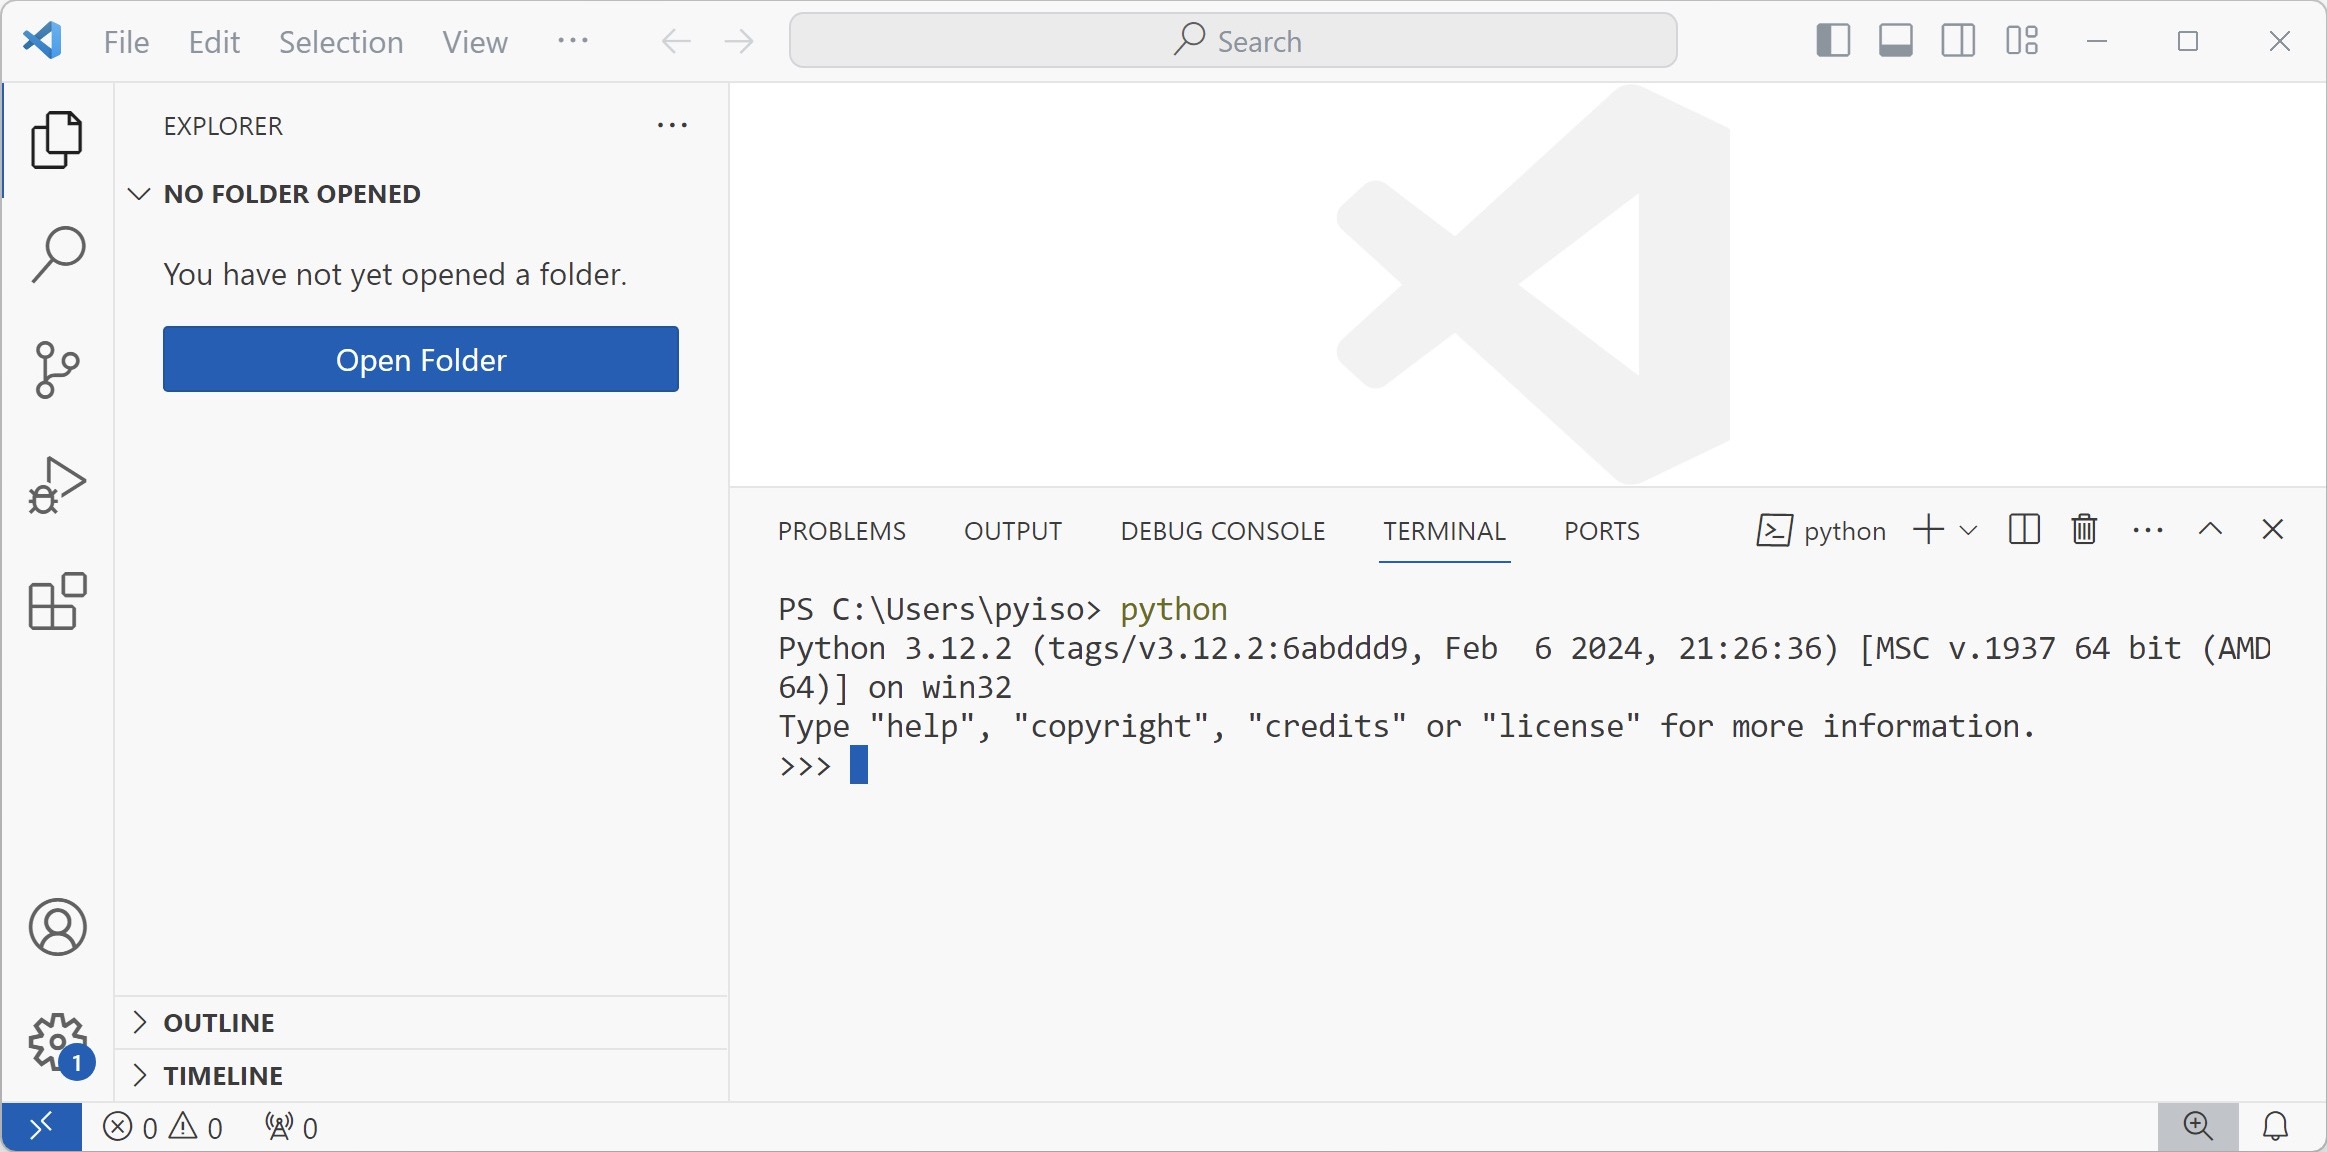
\includegraphics[width=.98\textwidth, trim={3mm 2mm 2mm 2.5mm},clip]{images/ch05/vscode py console.jpg}};
  \drawshadow{image}
\end{tikzpicture}
\caption{VS Code Python Console} 
\label{fig:vscconsole}
\end{figure}

\begin{figure}[tbh!]
\begin{tikzpicture}
  \node[anchor=south west,inner sep=0] (image) at (0,0)
  {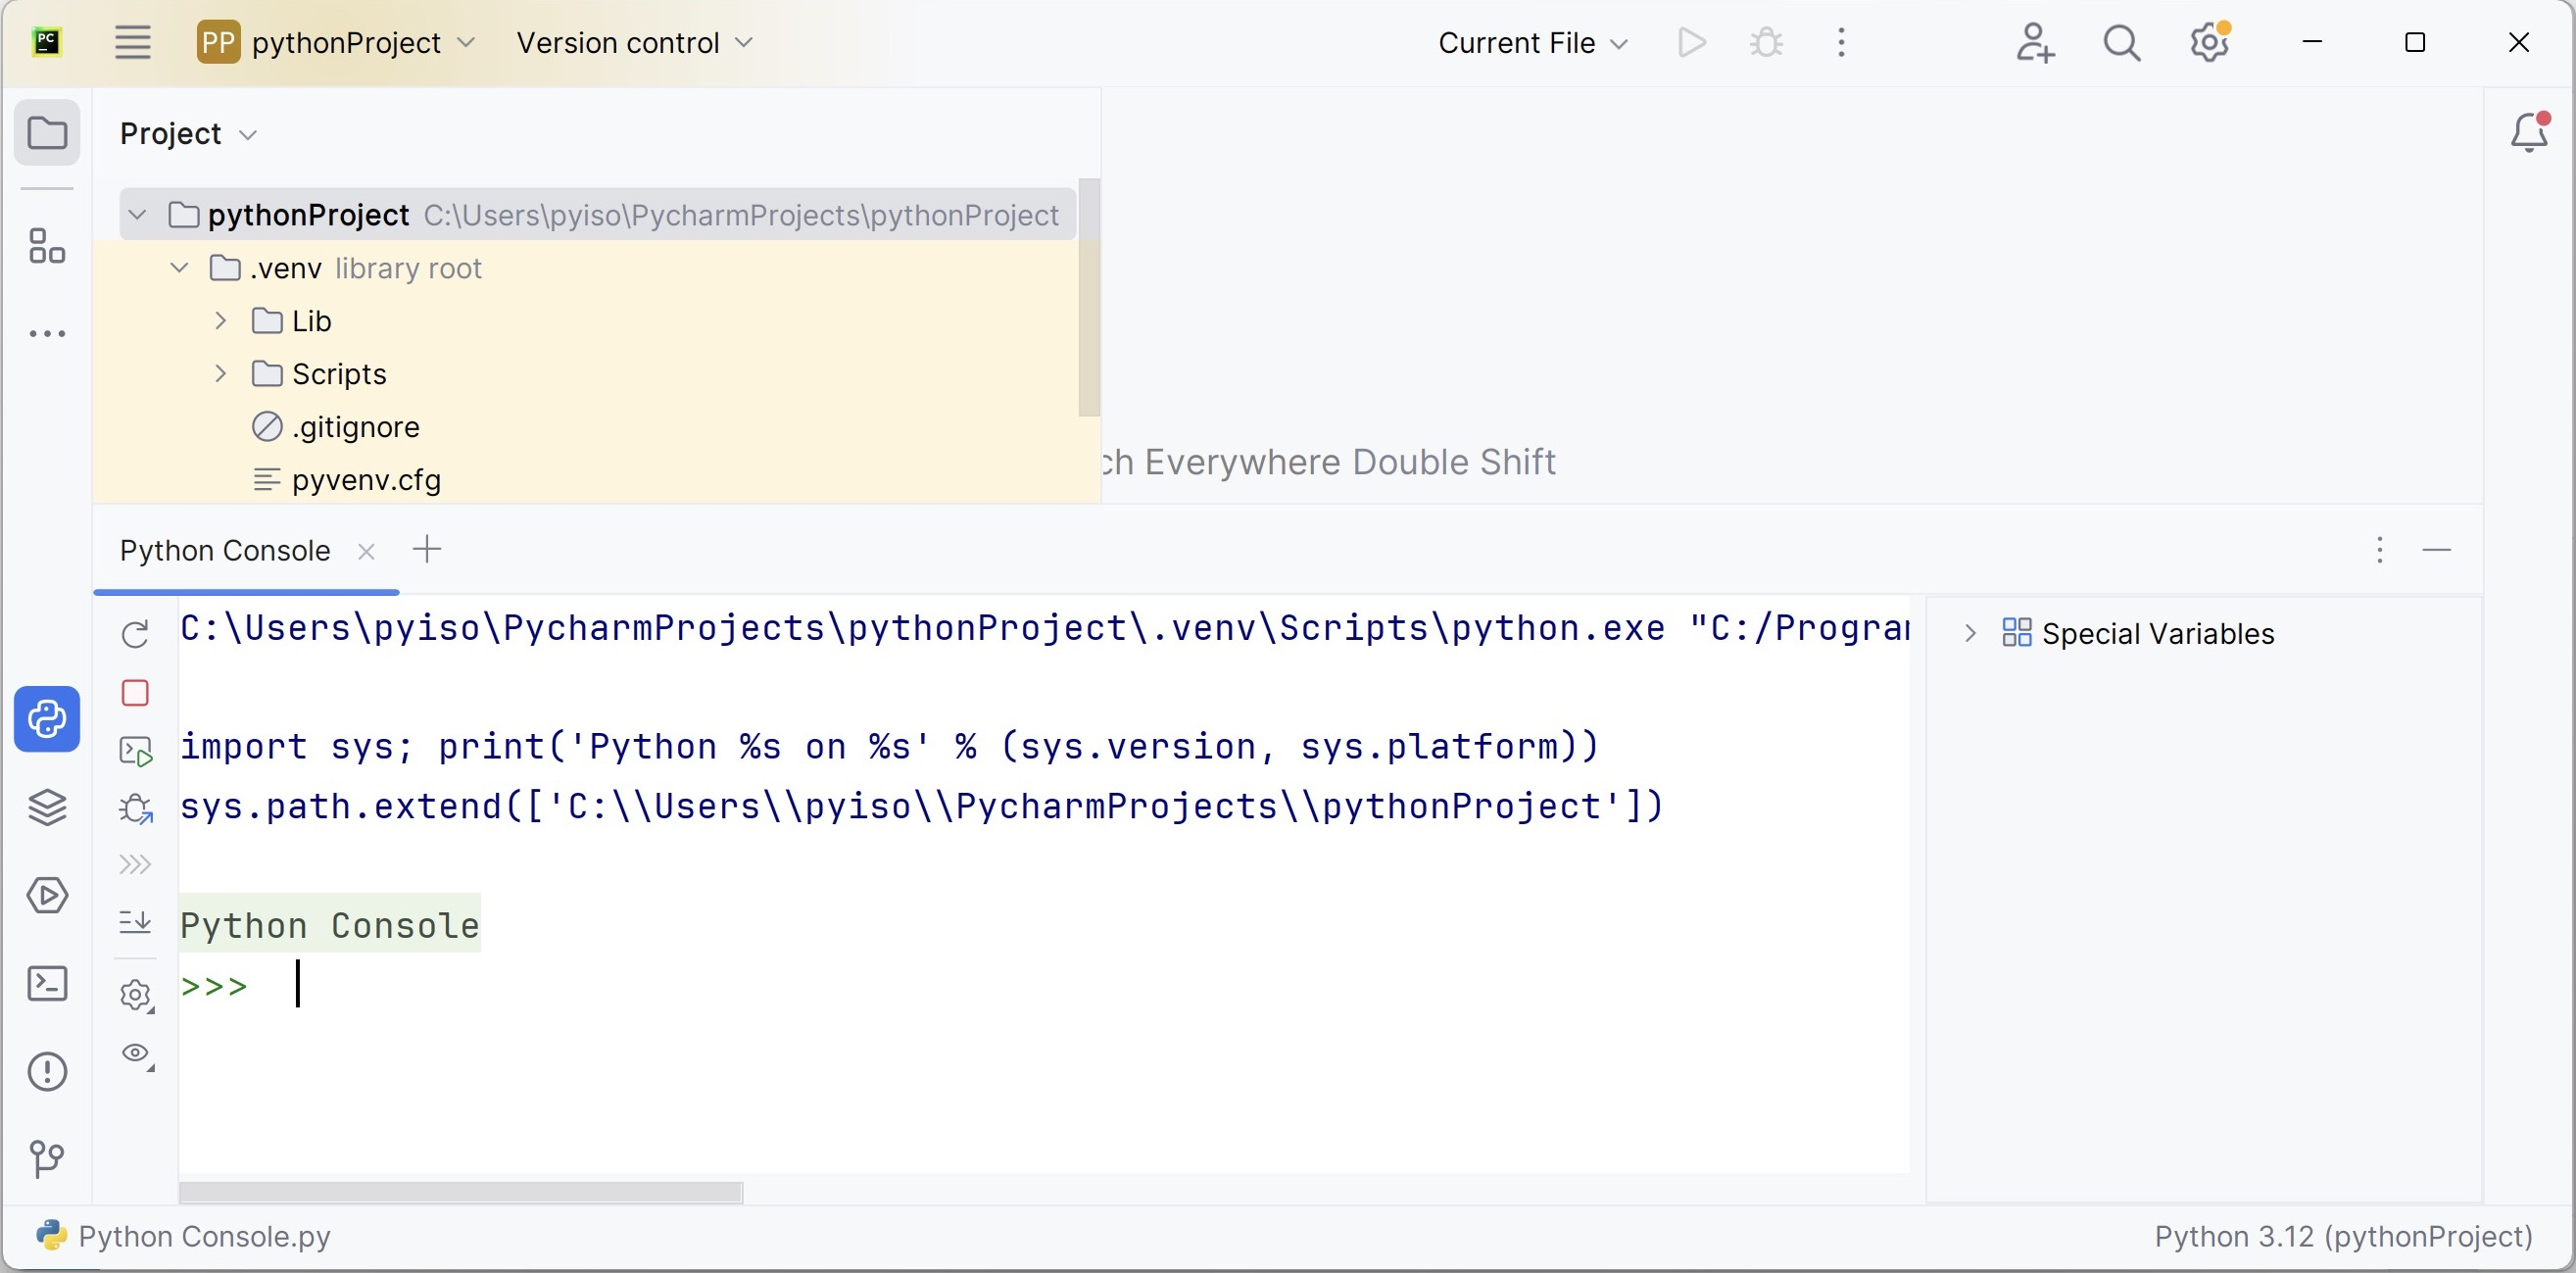
\includegraphics[width=.98\textwidth, trim={3mm 2mm 2mm 3.5mm},clip]{images/ch05/pycharm py console.jpg}};
  \drawshadow{image}
\end{tikzpicture}
\caption{PyCharm Python Console} 
\label{fig:pycharmconsole}
\end{figure}

\fCode{2 + 5} ထည့်ပြီး \fEn{Enter} ကီးနှိပ်ပါ။ အင်တာပရက်တာက ရလဒ် \fCode{7} နဲ့ တုံ့ပြန် လုပ်ဆောင်ပေးပါလိမ့်မယ်။ ဒီလို အင်တာပရက်တာက လုပ်ဆောင်ပေးတာကို  \fEnEmp{evaluate} လုပ်တယ်လို့ ပြောတယ်။
%
\setlength{\fboxsep}{0pt}
\begin{codetxt}
>>> 2 + 5
7
\end{codetxt}


%
အောက်ပါအတိုင်း တစ်ခုပြီးတစ်ခု ဆက်လက်စမ်းသပ်ကြည့်ပါ။
%
\setlength{\fboxsep}{0pt}
\begin{codetxt}
>>> 2 + 2
4
>>> 3 * 3
9
>>> 4 - 2
2
>>> 5/2
2.5
\end{codetxt}
%
$3 \times 3$ ကို \fCode{3 * 3} လို့ ရိုက်ထည့်ပေးရပြီး $5 \div 2$ အတွက် \fCode{5 / 2} လို့ ရေးရတာကို သတိပြုမိမှာပါ။ \fEn{Programming language} အများစုမှာ \fCode{*} \fEn{(asterisk)} အမြှောက်သင်္ကေတအဖြစ် အသုံးပြုပြီး \fCode{/} \fEn{(forward slash)} ကို အစားသင်္ကေတအနေနဲ့ အသုံးပြုလေ့ရှိတယ်။


\subsection*{Values and Types}
တန်ဖိုးတိုင်းဟာ တိုက်ပ် \fEn{(\textit{type})} တစ်မျိုးမျိုးမှာ ပါဝင်ပါတယ်။  \fCode{-3}\fEn{,} \fCode{0}\fEn{,} \fCode{2}  စတဲ့ တန်ဖိုးတွေဟာ \fCode{int} (\fEn{integer} ရဲ့ အတိုကောက်) တိုက်ပ်ဖြစ်ပြီး 
\fCode{-3.0}\fEn{,} \fCode{0.1}\fEn{,} \fCode{3.3333} စတာတွေက \fCode{float} တိုက်ပ် ဖြစ်ပါတယ်။ ဒဿမကိန်းတွေကို ကွန်ပျူတာနဲ့ ဖော်ပြဖို့ \fEnEmp{floating point} လို့ခေါ်တဲ့ နည်းစနစ်ကို အသုံးပြုတယ်။ ဒဿမကိန်း အတွက်အချက်တွေကိုလည်း ဒီနည်းစနစ်ကို အခြေခံပြီး ကွန်ပျူတာက လုပ်ဆောင်တာပါ။ ဒါကြောင့် \fEn{floating point} ဟာ ဒဿမကိန်းတွေကို ဖော်ပြဖို့နဲ့ ဒဿမကိန်း အတွက်အချက်တွေ လုပ်ဆောင်ဖို့ တီထွင်ထားတဲ့ နည်းစနစ်တစ်ခုလို့ ဆိုနိုင်ပါတယ်။ ဒီစနစ်ကို အခြေခံထားတဲ့ ဒဿမကိန်းတွေကို \fEn{programming language} တွေမှာ \fCode{float} တိုက်ပ်လို့ ခေါ်တာပါ။


\fCode{float} တိုက်ပ်ဟာ လိုသလောက် တိကျလို့မရတဲ့ သဘောရှိတယ်။ အောက်ပါအတိုင်း စမ်းကြည့်ရင်  \fCode{0.3} နဲ့ \fCode{1.0} ရသင့်တာ ဖြစ်ပေမဲ့ အတိအကျ အဖြေမထွက်ပါဘူး။
%
\setlength{\fboxsep}{0pt}
\begin{codetxt}
>>> 0.1 + 0.1 + 0.1
0.30000000000000004
>>> 0.1 + 0.1 + 0.1 + 0.1 + 0.1 + 0.1 + 0.1 + 0.1 + 0.1 + 0.1;
0.9999999999999999
\end{codetxt}
%
ကွာခြားချက်က မဆိုစလောက် သေးငယ်တယ် ဆိုပေမဲ့ ဒီအချက်ကို ပရိုဂရမ်မာ အနေနဲ့ ဂရုပြုမိဖို့ လိုပါတယ်။  \fEn{Floating point}  စနစ်ဟာ လုံးဝကြီးတိကျဖို့ မလိုအပ်တဲ့ (တနည်းအားဖြင့် မဆိုစလောက်သေးငယ်တဲ့ ကွာဟချက်ကို လက်ခံနိုင်တဲ့) ကိန်းဂဏန်းအတွက်အချက် ကိစ္စတွေအတွက် ရည်ရွယ်တာပါ။ သိပ္ပံနဲ့ နည်းပညာဆိုင်ရာ တိုင်းတာ တွက်ချက်မှုတွေအတွက် အသုံးပြုလေ့ရှိတယ်။ ဒဿမကိန်းတွေ လုံးဝအတိအကျ ဖြစ်ဖို့ လိုအပ်တဲ့ ကိစ္စမျိုးတွေ (ဥပမာအားဖြင့် ငွေကြေးကိစ္စ အတွက်အချက်) မှာ အသုံးမပြုသင့်ပါဘူး။ ဆယ်ပြားကို \fCode{0.1} နဲ့ဖော်ပြရင် ဆယ်ပြားစေ့ ဆယ်စေ့ဟာ တစ်ကျပ် ဖြစ်ကို ဖြစ်သင့်ပြီး \fCode{0.9999999999999999} မဖြစ်သင့်ဘူး။ ဒီလိုကိစ္စမျိုးတွေအတွက် \fEn{Python} မှာ \fCode{Decimal} ကို အသုံးပြုနိုင်ပါတယ်။  လောလောဆယ် ကိန်းဂဏန်းတွေနဲ့ ပါတ်သက်ပြီး စကတည်းက သိထားသင့်တာတချို့ကို ကြိုပြောထားတာပါ။ \fCode{Decimal} တိုက်ပ် အကြောင်း မကြာခင် လေ့လာမှာပါ။
%
\setlength{\fboxsep}{0pt}
\begin{codetxt}
>>> from decimal import *
>>> Decimal('0.1') + Decimal('0.1') + Decimal('0.1')
Decimal('0.3')
\end{codetxt}
%

 \fCode{int}  တိုက်ပ် ဖော်ပြနိုင်တဲ့ အကြီးဆုံး အပေါင်းကိန်းပြည့် သို့မဟုတ် အငယ်ဆုံး အနှုတ်ကိန်းပြည့် တန်ဖိုးကို ကန့်သတ်ထားတာ မရှိဘူး။  သီအိုရီအရ ကြိုက်သလောက် ကြီးလို့/ငယ်လို့ ရပါတယ်။ လက်တွေ့မှာတော့ အသုံးပြုတဲ့ ကွန်ပျူတာစနစ်ပေါ် မူတည်ပြီး ကန့်သတ်ချက်ရှိမှာပါ။ ဒီစာရေးနေတဲ့ ကွန်ပျူတာမှာ အောက်ပါကိန်းပြည့်တွေကို အသာလေး တွက်ချက်ပေးနိုင်ပါတယ်။ ဒီ့ထက်အများကြီး ကြီးတဲ့ဟာတွေကိုလည်း ကိုင်တွယ်တွက်ချက်နိုင်အုံးမှာပါ။ တော်ရုံကိစ္စတွေအတွက် ကွန်ပျူတာစနစ်တစ်ခုရဲ့ လက်တွေ့ကန့်သတ်ချက်ကို ကျော်လွန်သွားဖို့ မလွယ်ပါဘူး။
%
\setlength{\fboxsep}{0pt}
\begin{codetxt}
>>> 9000000000000000000000000000 + 5000000000
9000000000000000005000000000
>>> -9000000000000000000000000000 + 1 
-8999999999999999999999999999
 \end{codetxt}
 %
 
 \fCode{float} ကတော့ \fCode{int} နဲ့ မတူဘဲ အကြီးဆုံး/အငယ်ဆုံး ကန့်သတ်ချက်ရှိပါတယ်။ ဒီကန့်သတ်ချက်ကလည်း ကွန်ပျူတာစနစ်ပေါ် မူတည်ပါတယ်။ တစ်ကိုယ်ရေသုံး ကွန်ပျူတာ အများစုအတွက် \(1 \times 10^{400}\) (၁ နောက် သုည အလုံး ၄၀၀) သို့မဟုတ် \(-1 \times 10^{400}\) (အနှုတ် ၁ နောက် သုည အလုံး ၄၀၀) ဟာ ကန့်သတ်ချက်ကျော်လွန်ပါတယ်။ 
%
\setlength{\fboxsep}{0pt}
\begin{codetxt}
>>> 1e400
inf
>>> -1e400
-inf
>>> 1e-400
0.0
>>> -1e-400
-0.0
 \end{codetxt}
 %
 ဒဿမကိန်းကို \fEnEmp{e} အမှတ်အသားနဲ့ရေးထားတာပါ။  အက္ခရာ \fCode{e} နောက် လိုက်တဲ့ ကိန်းပြည့်ဂဏန်းကို $10$ ထပ်ကိန်းလို့ မှတ်ယူရပါတယ်။ \fCode{e3} က \(1 \times 10^{3}\)\fEn{,} \fCode{e-3} က \(1 \times 10^{-3}\) ပါ။ အက္ခရာ \fEnEmp{E} အကြီးနဲ့လည်း ရေးနိုင်တယ်။ ထပ်ကိန်း ကြီးလွန်းတဲ့အတွက် ကန့်သတ်ချက် ကျော်လွန်ရင် \fCode{inf} (အနှုတ်ကိန်းဆိုရင် \fCode{-inf} ) ရပါမယ်။ \fEn{Infinity} ကို ဆိုလိုတာပါ။ (၁) မပြည့်တဲ့ ပမာဏ သေးငယ်လွန်းတဲ့ ဂဏန်းတွေကိုလည်း အနီးစပ်ဆုံး သုညအနေနဲ့ ယူပါတယ်။ အနီးစပ်ဆုံးယူတဲ့အခါ အပေါင်း/အနှုတ်ကိုတော့ ခွဲခြားပေးပါတယ်။ \fEnEmp{e} အမှတ်အသားနဲ့ရေးထားတဲ့ နောက်ထပ် ဥပမာလေး နှစ်ခုပါ
%
\setlength{\fboxsep}{0pt}
\begin{codetxt}
7.34767309e22    # mass of the moon in kg
9.1093837015e-31 # mass of an electron in kg
\end{codetxt}
%

ဂဏန်းအလုံးအရေအတွက် များရင် $100,500$ (တစ်သိန်းငါးရာ)၊ $1,500,000$ (တစ်သန်းငါးသိန်း) စသဖြင့် သုံးလုံးတစ်ဖြတ် ကော်မာခံရေးလေ့ရှိတယ်။ \fEn{Python} မှာတော့ ကော်မာအစား \fEn{\textunderscore (underscore)} နဲ့ သုံးလုံးတစ်ဖြတ် ခြားရေးနိုင်ပါတယ်။ 
%
\setlength{\fboxsep}{0pt}
\begin{codetxt}
>>> 1_500_000 + 100_500
1600500
>>> 200_000.33 + 3_800_000.22
4000000.5500000003
\end{codetxt}
%



\subsection*{တိုက်ပ်မတူသည့် ကိန်းဂဏန်း အိပ်စ်ပရက်ရှင်များ}
အိပ်စ်ပရက်ရှင်တွေမှာ ပါဝင်တဲ့ တိုက်ပ် တစ်မျိုးတည်း ဖြစ်ရမယ် မရှိပါ။ တိုက်ပ်မတူတဲ့ ကိန်းဂဏန်းတွေ အိပ်စ်ပရက်ရှင်တစ်ခုမှာ ရောပြီး ပါဝင်နိုင်ပါတယ်။
%
\setlength{\fboxsep}{0pt}
\begin{codetxt}
>>> 5 - 2.0
3.0
>>> 5 - 2
3
>>> 3 * 2.0
6.0
>>> 3 * 2
6
\end{codetxt}
%
\fCode{int} နဲ့ \fCode{float} ရောနေရင် အိပ်စ်ပရက်ရှင် ရလဒ်သည် \fCode{float} တိုက်ပ် ဖြစ်မှာပါ။ အစား \fEn{(division)} မှာတော့ အင်တီဂျာအချင်းချင်း စားတဲ့အခါမှာလည်း ရလဒ်က \fCode{float} ဖြစ်ပါမယ်။ 
%
\setlength{\fboxsep}{0pt}
\begin{codetxt}
>>> 9/3
3.0
>>> 9.12/3.3
2.7636363636363637
>>> 88/3
29.333333333333332
>>> 1/3
0.3333333333333333
>>>
\end{codetxt}
%

\subsection*{အင်တီဂျာ ဒီဗီးရှင်း၊ မော်ဒျူလို နှင့် ထပ်ကိန်းတင်ခြင်း}
အကယ်၍ ဒဿမကိန်းမထွက်ဘဲ ကိန်းပြည့် လိုချင်ရင် \fCode{//} ကို သုံးရပါမယ်။ ဒီအခါ အကြွင်းကိုဖယ်ပြီး စားလဒ်ကိုပဲ ကိန်းပြည့်အနေနဲ့ ရမှာပါ။ 
%
\setlength{\fboxsep}{0pt}
\begin{codetxt}
>>> 9//3
3
>>> 12//5
2
>>> 3//5
0
\end{codetxt}
%
သင်္ချာမှာ ဒီလိုမျိုး အစားကို အင်တီဂျာ ဒီဗီးရှင်း \fEn{(integer division)} လို့ခေါ်ပါတယ်။ အကြွင်းရှာမယ်ဆိုရင် \mintinline{text}|%| အော်ပရိတ်တာ ရှိပါတယ်။ \mintinline{text}|%| ကို မော်ဒျူလို \fEn{(modulo)} အော်ပရိတ်တာလို့ ခေါ်တယ်။ \fEn{remainder} အော်ပရိတ်တာလို့လည်း ခေါ်တယ်။ 
%
\setlength{\fboxsep}{0pt}
\begin{codetxt}
>>> 7 % 5
2
>>> 100 % 10
0
\end{codetxt}
%

အင်တီဂျာ ဒီဗီးရှင်းနဲ့ မော်ဒျူလိုကို အနှုတ်ကိန်းတွေနဲ့ သုံးမယ်ဆိုရင် သတိပြုပါ။  စားလဒ် အနှုတ်ကိန်း ဖြစ်ရင် \fCode{//} က ပိုငယ်တဲ့ အနှုတ်ကိန်းကို အနီးစပ်ဆုံး ယူမှာပါ။ တစ်နည်းအားဖြင့် \fEn{round down} လုပ်တာ ဖြစ်တယ်။
%
\setlength{\fboxsep}{0pt}
\begin{codetxt}
>>> -12 // -10
1
>>> -12 // 10
-2
>>> 12 // -10
-2
>>> -31 // 10
-4
>>> -35 // 10
-4
>>> -38 // 10
-4
\end{codetxt}
%
\fCode{-2} နဲ့ \fCode{-4} ထွက်တာ သတိပြုပါ။ အဖြေအတိအကျက \fCode{-1.2} ကို အနီးစပ်ဆုံး သူ့ထက်ပိုငယ်တဲ့ \fCode{-2} ကို အနီးစပ်ဆုံး ယူတယ်။ \fCode{-3.1}\fEn{,} \fCode{-3.5}\fEn{,} \fCode{-3.8} တို့ကိုလည်း အနီးစပ်ဆုံး \fCode{-4} ယူတာပါ။

မော်ဒျူလို အော်ပရိတ်တာ \mintinline{text}|%| သုံးတဲ့အခါ ရလဒ်ဟာ စားကိန်းရဲ့ \fEn{sign} အပေါ် မူတည်တယ်။ (အပေါင်း အနှုတ်ကို ဆိုလိုတာပါ)။ 
%
\setlength{\fboxsep}{0pt}
\begin{codetxt}
>>> -17 % 10
3
>>> 17 % -10
-3
\end{codetxt}
%
မော်ဒျူလိုနဲ့ အင်တီဂျာ ဒီဗီးရှင်း အော်ပရိတ်တာ နှစ်ခုက အောက်ပါညီမျှခြင်းအရ ဆက်စပ်နေတာပါ။ စားကိန်း $B \neq 0$ ဖြစ်ပါတယ်။
\[
  B * (A // B) + A \SI{}{\fEn{\percent}} B = A
\]
ဒါကြောင့် $B = 10, A = -17$ ဖြစ်လျှင် 
\begin{align*}
B * (A//B) + A \SI{}{\fEn{\percent}} B &= A &\\
10 * (-17//10) + -17 \SI{}{\fEn{\percent}} 10 &= -17 &\\
-20 + -17 \SI{}{\fEn{\percent}} 10 &= -17 &\\
-17 \SI{}{\fEn{\percent}} 10 &= -17 + 20 &\\
-17 \SI{}{\fEn{\percent}} 10 &= 3 &
\end{align*}
အကယ်၍ $B = -10, A = 17$ ဖြစ်လျှင်
\begin{align*}
B * (A//B) + A \SI{}{\fEn{\percent}} B &= A&\\
-10 * (17//-10) + 17 \SI{}{\fEn{\percent}} -10 &= 17&\\
20 + 17 \SI{}{\fEn{\percent}} -10 &= 17&\\
17 \SI{}{\fEn{\percent}} -10 &= 17 - 20&\\
17 \SI{}{\fEn{\percent}} -10 &= -3 &
\end{align*}

အထက်ပါ ညီမျှခြင်းဟာ ကိန်းပြည့်တွေအတွက်ပဲ မှန်တာပါ။ \fCode{//} နဲ့ \mintinline{text}|%|  ကို ဒဿမကိန်းတွေနဲ့လည်း သုံးလို့ရပေမဲ့ ရလဒ်တွေက အထက်ပါ ညီမျှခြင်းကို ပြေလည်စေမှာ မဟုတ်ပါဘူး။ \fCode{float} တိုက်ပ်ဟာ 
%
\setlength{\fboxsep}{0pt}
\begin{codetxt}
>>> 9.9 // 3.3
3.0
>>> 9.9 % 3.3
8.881784197001252e-16
>>> 9.9 / 3.3
3.0000000000000004
>>> 3.5 / 0.1
35.0
>>> 3.5 // 0.1
34.0
>>> 3.5 % 0.1
0.09999999999999981
\end{codetxt}
%


ထပ်ကိန်းတင် \fEn{(exponentiation)} ဖို့ အတွက် အော်ပရိတ်တာက \fCode{**}  ပါ။ $2^4$ နဲ့ $(3.3)^3$ ကို အခုလို တွက်ပါတယ်။
%
\setlength{\fboxsep}{0pt}
\begin{codetxt}
>>> 2 ** 4
16
>>> 3.3 ** 3
35.937
\end{codetxt}
%

\subsection*{သင်္ချာဖန်ရှင်များ}
ကိန်းဂဏန်းတွေအကြောင်း လေ့လာလက်စနဲ့ \fCode{math} လိုက်ဘရီ သင်္ချာဖန်ရှင်တချို့ကိုလည်း တစ်ခါတည်း ဆက်ကြည့်လိုက်ရအောင်။ အဓိကက သင်္ချာဖန်ရှင်ဆိုတာထက် ဖန်ရှင် အခြေခံအသုံးပြုပုံကို စပြီးလေ့လာမှာပါ။ \fCode{math} လိုက်ဘရီက \fEn{Python} မှာ တစ်ခါတည်း ထည့်ထားပေးပြီးသား \fEn{(built-in)} လိုက်ဘရီပါ။ အင်စတောလ်လုပ်စရာ မလိုဘဲ အင်ပို့လုပ်ပြီး သုံးလို့ရတယ်။
\begin{codetxt}
>>> from math import *
\end{codetxt}
အင်ပို့လုပ်ပြီးရင် \fCode{math} လိုက်ဘရီဖန်ရှင်တွေကို သုံးလို့ရပါပြီ။ ကိန်းတစ်ခုရဲ့ နှစ်ထပ်ကိန်းရင်းကို \fCode{sqrt}\fEn{,} သုံးထပ်ကိန်းရင်းကို \fCode{cbrt} ဖန်ရှင်နဲ့ ရှာနိုင်ပါတယ်။
\begin{codetxt}
>>> cbrt(27)
3.0
>>> sqrt(81)
9.0  
\end{codetxt}

သင်္ချာဖန်ရှင်အားလုံးဟာ \fEn{input} တန်ဖိုးတစ်ခု သို့မဟုတ် တစ်ခုထက်ပို၍ လက်ခံပြီး \fEn{output} တန်ဖိုးတစ်ခု ပြန်ထုတ်ပေးပါတယ်။ \fCode{27} နဲ့  \fCode{81} ဟာ \fEn{input} ဖြစ်ပြီး \fCode{3.0} နဲ့  \fCode{9.0} က \fEn{output} ဖြစ်တယ်။
\begin{codetxt}
>>> gcd(2406, 654)
6
>>> gcd(2406, 654, 354)
6
>>> gcd(2406)
2406
\end{codetxt}
အကြီးဆုံးဘုံဆခွဲကိန်းကို \fCode{gcd} ဖန်ရှင်နဲ့ ရှာတာပါ။ အင်တီဂျာ \fEn{input} တစ်ခုနဲ့အထက် လက်ခံတဲ့ ဖန်ရှင်ဖြစ်တယ်။ \fEn{input} ဂဏန်းအားလုံးကို စားလို့ပြတ်တဲ့ အကြီးဆုံးကိန်းကို ရှာပေးတယ်။ ကိန်းပြည့်မဟုတ်တာ ထည့်ရင် အယ်ရာဖြစ်ပါတယ်။
\begin{codetxt}
>>> gcd(2.4, 4.8)
Traceback (most recent call last):
  File "<stdin>", line 1, in <module>
TypeError: 'float' object cannot be interpreted as an integer
\end{codetxt}

လော့ဂရစ်သမ်၊ ထရီဂိုနိုမေထရီ ဖန်ရှင်တွေလည်းပါတယ်။ $\log_{10}(x)$\fEn{,} $\sin(x)$\fEn{,} $\cos(x)$ တို့ကို ဥပမာပြထားတာ ကြည့်ပါ။
\begin{codetxt}
>>> log10(1000)
3.0
>>> sin(pi/2) # pi/2 radians = 90 degrees
1.0
>>> sin(pi/4) ** 2 + cos(pi/4) ** 2
1.0
\end{codetxt}


\section{‘တိုက်ပ်’ ဆိုတာ ဘာလဲ}
\fEn{Programming language} အားလုံးမှာ တိုက်ပ် သို့မဟုတ် ဒေတာတိုက်ပ် သဘောတရား ပါရှိပါတယ်။ \fCode{int} နဲ့ \fCode{float} တိုက်ပ်မှာ ပါဝင်တဲ့ ကိန်းပြည့်တွေနဲ့ ဒဿမကိန်းတွေကို မိတ်ဆက်ပြီးတဲ့အခါ ‘တိုက်ပ်’ ဆိုတာဘာလဲ တိတိကျကျ ရှင်းပြလို့ရပါပြီ။ တိုက်ပ်တစ်ခုဟာ
%
\begin{itemize}
  \item တန်ဖိုးတွေပါဝင်တဲ့ အစု \fEn{(set)} တစ်ခု နဲ့
  \item ၎င်းတန်ဖိုးများအပေါ်တွင် အသုံးချနိုင်တဲ့ အော်ပရေးရှင်းတွေ ပါဝင်တဲ့ အစုတစ်ခု
\end{itemize}
%
ဖြစ်ပါတယ်။ ဥပမာ \fCode{int} တိုက်ပ်ကို ကြည့်ရင် ကိန်းပြည့်တွေ ပါဝင်တဲ့ အစုနဲ့ ကိန်းပြည့်တွေအပေါ်မှာ လုပ်ဆောင်လို့ရတဲ့  အော်ပရေးရှင်းတွေ ပါဝင်တဲ့ အစု
%
\begin{align*}
& \{\ldots , -3, -2, -1, 0, 1, 2, 3, \ldots \} &\\
& \{+, -, *, /, //, \SI{}{\fEn{\percent}}, **, \ldots \} &%
\end{align*}
ဖြစ်ပါတယ်။ \fCode{float} တိုက်ပ်ကတော့ ကိန်းစစ် \fEn{(real numbers)} တွေပါဝင်တဲ့ အစုနဲ့ ၎င်းတို့အပေါ်မှာ လုပ်ဆောင်လို့ရတဲ့  အော်ပရေးရှင်းတွေ ပါဝင်တဲ့ အစုတို့ ဖြစ်ပါတယ်။ \fCode{int} နဲ့ \fCode{float} တိုက်ပ်မှာ အော်ပရေးရှင်းတွေ တူတူဖြစ်နေတာ တွေ့ရမှာပါ။ ဒီလိုအမြဲဖြစ်မယ်လို့ မယူဆရပါဘူး။ တိုက်ပ် မတူတဲ့အခါ အသုံးချလို့ ရနိုင်တဲ့ အော်ပရေးရှင်းတွေ ကွာခြားနိုင်ပါတယ်။ ဥပမာ \fCode{str} တိုက်ပ် အော်ပရေးရှင်းတွေက \fCode{int} တို့ \fCode{float} တို့နဲ့ မတူပါဘူး။ \fCode{str} က \fEnEmp{string} ရဲ့ အတိုကောက်ဖြစ်ပြီး စာသားတွေအတွက် အသုံးပြုပါတယ်။ မကြာခင် လေ့လာကြမှာပါ။

အပေါ်က အော်ပရေးရှင်း အစုမှာ အစက်သုံးစက် $‘\ldots’$ ကို သတိပြုပါ။ ဆိုလိုတာက အခြား အော်ပရေးရှင်းတွေ ဒီအစုမှာ ပါဝင်ပါသေးတယ်။ \fCode{int} နဲ့ \fCode{float} တွေအတွက် ဖန်ရှင်တွေကိုလည်း ဒီအစုမှာ ပါဝင်တယ်လို့ ယူဆရမှာပါ။
%
\setlength{\fboxsep}{0pt}
\begin{codetxt}
>>> from math import *
>>> sqrt(2.0)
1.4142135623730951
>>> abs(-5)
5
\end{codetxt}
% 
ဥပမာအနေနဲ့ \fCode{sqrt} နဲ့ \fCode{abs} ဖန်ရှင် အသုံးချပုံပါ။ နှစ်ထပ်ကိန်းရင်းနဲ့ ပကတိတန်ဖိုး ရှာပေးပါတယ်။ လိုအပ်ရင် ကိုယ်ပိုင်ဖန်ရှင်တွေ သတ်မှတ်ပြီး တိုက်ပ်တစ်ခုရဲ့ အော်ပရေးရှင်းတွေကို ဖြည့်စွက်တိုးချဲ့နိုင်ပါတယ်။

\begin{mytcbox}
အော်ပရေးရှင်းနဲ့ အော်ပရိတ်တာ ရောထွေးစရာ ရှိပါတယ်။ $+, -, *, /, //, \SI{}{\fEn{\percent}}, **$ စတဲ့ သင်္ကေတတွေကို အော်ပရိတ်တာလို့ ခေါ်ပါတယ်။ အော်ပရေးရှင်း လုပ်ဆောင်ဖို့အတွက် အသုံးပြုတဲ့ သင်္ကေတတွေကို အော်ပရိတ်တာလို့ ခေါ်တာပါ။ ဥပမာ “$*$ သင်္ကေတဟာ အမြှောက်အော်ပရေးရှင်း လုပ်ဆောင်ဖို့ သတ်မှတ်ထားတဲ့ အော်ပရိတ်တာ” လို့ ပြောတယ်။ အမြှောက်  ‘အော်ပရေးရှင်း’ ကျတော့ မြှောက်တဲ့အလုပ် ဆောက်ရွက်တာကို ဆိုလိုတာ။
\end{mytcbox}


\section{ဗေရီရေဘဲလ်များ}
ဗေရီရေဘဲလ်ဆိုတာ တန်ဖိုးတစ်ခုကို ကိုယ်စားပြုတဲ့ နံမည်ပါပဲ။ နံမည်နဲ့ ၎င်းကိုယ်စားပြုတဲ့ တန်ဖိုး တွဲဖက်ပေးဖို့ အဆိုင်းမန့် \fEn{(\textit{assignment})} စတိတ်မန့်ကို သုံးရပါတယ်။
%
\setlength{\fboxsep}{0pt}
\begin{codetxt}
>>> age = 12
>>> weight = 35.5
\end{codetxt}
%
\fCode{age} နဲ့ \fCode{weight} ဟာ ဗေရီရေဘဲလ်တွေ ဖြစ်ပါတယ်။   ညီမျှခြင်းသင်္ကေတ (\fCode{=}) ကတော့ အဆိုင်းမန့် အော်ပရိတ်တာပါ။ ဗေရီရေဘဲလ်နဲ့ တန်ဖိုး တွဲဖက်ပေးတဲ့ အော်ပရိတ်တာ ဖြစ်တယ်။ ဗေရီရေဘဲလ်နံမည်ကို \fEn{variable} \fEnEmp{identifier} လို့လည်း ခေါ်ပါတယ်။ \fEn{Identifier} က နည်းပညာ အခေါ်အဝေါ်ပေါ့။ \fEn{Variable name} က သာမန်လူ နားလည်တဲ့ နည်းနဲ့ ပြောတာပါ။ ဗေရီရေဘဲလ် တစ်ခုချင်း ထည့်ကြည့်ရင် ၎င်းကိုယ်စားပြုတဲ့ တန်ဖိုးကို ပြန်ထုတ်ပေးတာ တွေ့ရမှာပါ။
%
\setlength{\fboxsep}{0pt}
\begin{codetxt}
>>> age
12
>>> weight
35.5
\end{codetxt}

%
အိပ်စ်ပရက်ရှင်တွေက ဗေရီရေဘဲလ်တွေနဲ့ ဖြစ်နိုင်ပါတယ်။ အိပ်စ်ပရက်ရှင် တွက်ချက်ရင် ဗေရီရေဘဲလ် တန်ဖိုးနဲ့ အစားထိုး တွက်ချက်တယ်လို့ ယူဆရမှာပါ။ ဥပမာ
%
\setlength{\fboxsep}{0pt}
\begin{codetxt}
>>> age + 1
13
>>> weight / 2
17.75
\end{codetxt}
%
ဗေရီရေဘဲလ်တစ်ခုကို အိပ်စ်ပရက်ရှင်ရလဒ်နဲ့ အဆိုင်းမန့် လုပ်လို့ရပါတယ်။ \fCode{rect\_area} ကို အောက်တွင် ကြည့်ပါ။ အလျား အနံ မြှောက်လဒ်ကို အဆိုင်းမန့် လုပ်ထားတာ တွေ့ရပါမယ်။
%
\setlength{\fboxsep}{0pt}
\begin{codetxt}
>>> rect_width = 22.5
>>> rect_length = 10
>>> rect_area = rect_width * rect_length
>>> rect_area
225.0
\end{codetxt}
%


\subsection*{အဆိုင်းမန့် စတိတ်မန့်}
ဗေရီရေဘဲလ်တစ်ခုဟာ အချိန်တစ်ချိန်မှာ တန်ဖိုးတစ်ခုကိုပဲ ကိုယ်စားပြုနိုင်တယ်။ ဒါပေမဲ့ အချိန်ကာလပေါ် မူတည်ပြီး တန်ဖိုးပြောင်းနိုင်တယ်။ (တစ်ချိန်တည်းမှာ တန်ဖိုးနှစ်ခု မဖြစ်နိုင်ဘူး)။ ဥပမာ \fCode{x} တန်ဖိုးဟာ ပထမ \fCode{10} ပါ။ ဒုတိယ အဆိုင်းမန့်လုပ်ပြီးတဲ့ အချိန်မှာ အဲ့ဒီ \fCode{x} ကပဲ \fCode{1000} ဖြစ်နေမှာပါ။ 
%အဆိုင်းမန့် စတိတ်မန့်မှာ \fEn{identifier} က အသစ်ဖြစ်နိုင်သလို ရှိပြီးသားလည်း ဖြစ်နိုင်ပါတယ်။ 
%
\setlength{\fboxsep}{0pt}
\begin{codetxt}
>>> x = 10
>>> x
10
>>> x = 1000
>>> x
1000
\end{codetxt}
%

\section{စာသားများ}
စာသား \fEn{(text)} ဟာ အသုံးအများဆုံး ဆက်သွယ်ဆောင်ရွက်ရေး ကြားခံနယ်တစ်ခုပါ။ ဝက်ဘ်ဆိုက် စာမျက်နှာ၊ အီးမေးလ်၊ အီးဘွတ်ခ်နဲ့ အီလက်ထရွန်းနစ် စာရွက်စာတမ်း \fEn{(e-documents)} စတာတွေမှာ ရုပ်သံတွေ အသုံးပြုလာကြပေမဲ့ စာသား အဓိကဖြစ်နေဆဲပါပဲ။ ဆိုရှယ်မီဒီယာ၊ ဂိမ်းနဲ့ အခြားအပ်ပ်တွေ ဟာလည်း စာသားနဲ့ မကင်းနိုင်ကြပါဘူး။ ဒါကြောင့် ပရိုဂရမ်းမင်းအတွက် စာသားဟာ  ဘယ်လောက်ထိ အရေးပါကြောင်း အများကြီးပြောစရာ လိုမယ်မထင်ပါဘူး။ 

ပရိုဂရမ်းမင်းမှာ စာသားကို \fEnEmp{string} လို့ခေါ်ပြီး ကာရက်တာ \fEn{(\textit{character})} တွေနဲ့ စီတန်းဖွဲ့စည်းထားတယ်။ ကာရက်တာဆိုတာ အခြေခံ သတင်းအချက်အလက် ယူနစ်တစ်ခုပါပဲ။ အက္ခရာ၊ ဂဏန်း \fEn{(digit)}၊ သင်္ကေတ သို့မဟုတ် ကွန်ထရိုးလ်ကုဒ် တစ်ခုခု ဖြစ်နိုင်ပါတယ်။ ဥပမာ \fEn{A, B, C, \$, @, \#, 1, 3, \_ } စသည်ဖြင့်။ \fEn{Double quotes(}\fCode{"}\fEn{)} တစ်စုံကြား ညှပ်ရေးထားတဲ့ ကာရက်တာတွေ အသီအတန်းလိုက်ကို စာသားအနေနဲ့ ယူဆတယ်။ \fEn{Python} မှာ စာသားရဲ့ တိုက်ပ်ဟာ \fCode{str} ဖြစ်တယ်။ \fEn{string} ကို အတိုကောက် ယူထားတာပါ။ 
%
\setlength{\fboxsep}{0pt}
\begin{codetxt}
>>> "Hello, World!"
'Hello, World!'
\end{codetxt}
%
သို့မဟုတ် \fCode{"} အစား \fEn{single quotes(}\fCode{'}\fEn{)} တစ်စုံလည်း သုံးနိုင်ပါတယ်။ 
%
\setlength{\fboxsep}{0pt}
\begin{codetxt}
>>> 'Hello, World!'
'Hello, World!'
\end{codetxt}
%

စာသားတစ်ခုမှာ ပါဝင်တဲ့ ကာရက်တာ အရေအတွက်ကို \fCode{len} ဖန်ရှင်နဲ့ စစ်ကြည့်နိုင်ပါတယ်။ ကာရက်တာ တစ်လုံးမှ မပါတဲ့ \fCode{""} (သို့ \fCode{''}) ကို \fEn{empty string} လို့ ခေါ်ပါတယ်။ 
%
\setlength{\fboxsep}{0pt}
\begin{codetxt}
>>> len("Hello, World!")
13
>>> long_sentence = "This is a long sentence nobody wants to read."
>>> len(long_sentence)
45
>>> len("")
0
>>> len(" ") # contain a single space
1
\end{codetxt}
%

\fCode{str} တိုက်ပ်ရဲ့ အခြေခံကျတဲ့ အော်ပရေးရှင်းတစ်ခုက စာသားတစ်ခုနဲ့ တစ်ခု ဆက်တာပါ။ \fCode{+} အော်ပရိတ်တာနဲ့ စာသားတွေကို ဆက်နိုင်ပါတယ်။ 
%အော်ပရိတ်တာတစ်ခုဟာ တွဲဖက်အသုံးပြုတဲ့ \fEn{operand} တွေရဲ့ တိုက်ပ်ပေါ်မူတည်ပြီး လုပ်ဆောင်တဲ့ အော်ပရေးရှင်း  \todo{ကိန်းဂဏန်းစက်ရှင်တွင် ကြိုရှင်းရန်}
%
\setlength{\fboxsep}{0pt}
\begin{codetxt}
>>> "Yangon " + "and " + "Mandalay"
'Yangon and Mandalay'
\end{codetxt}
%
စာသားအချင်းချင်းပဲ ဆက်လို့ရပါတယ်။ စာသားနဲ့ ကိန်းဂဏန်း ဆက်လို့မရပါဘူး။ အောက်ပါအတိုင်း စမ်းကြည့်တဲ့အခါ \fCode{str} နဲ့ \fCode{float} ဆက်လို့မရဘူးလို့ အယ်ရာ\fOpn{မက်ဆေ့ချ်} ကျလာမှာပါ။
%
\setlength{\fboxsep}{0pt}
\begin{codetxt}
>>> from math import *
>>> pi
3.141592653589793
>>> "The value of π is " + pi
Traceback (most recent call last):
  File "<stdin>", line 1, in <module>
TypeError: can only concatenate str (not "float") to str
\end{codetxt}
%
\fCode{str} ဖန်ရှင်က ကိန်းဂဏန်းတစ်ခုကနေ စာသားကို ထုတ်ပေးပါတယ်။ မူရင်းကိန်းဂဏန်းကို စာသားဖြစ်အောင် ပြောင်းလိုက်တာ မဟုတ်ပါဘူး။ ကိန်းဂဏန်း တန်ဖိုးကနေ ၎င်းကိုဖော်ပြတဲ့ စာသားကို ဖန်ရှင်က ပြန်ထုတ်ပေးတာပါ။ 
%
\setlength{\fboxsep}{0pt}
\begin{codetxt}
>>> str(pi)
'3.141592653589793'
\end{codetxt}
%
ထွက်လာတဲ့ တန်ဖိုးဟာ စာသားဖြစ်တဲ့အတွက် \fEn{single quote} ပါနေတာ သတိပြုပါ။ \fCode{pi} တန်ဖိုးနဲ့ စာသား အခုလို ဆက်ရပါမယ်။ 
%
\setlength{\fboxsep}{0pt}
\begin{codetxt}
>>> "The value of π is " + str(pi)
'The value of π is 3.141592653589793'
\end{codetxt}
%
\fCode{str} ဖန်ရှင်နဲ့ စာသားရအောင် အရင်လုပ်ပြီးမှ ဆက်ထားတာပါ။

စာသားကနေ ကိန်းဂဏန်း လိုချင်ရင် \fCode{int} နဲ့ \fCode{float} ဖန်ရှင် သုံးနိုင်ပါတယ်။
%
\setlength{\fboxsep}{0pt}
\begin{codetxt}
>>> int('1024')
1024
>>> int('1024') * 2
2048
>>> float('2.4') * 3
7.199999999999999
\end{codetxt}
%
ဂဏန်းပြောင်းလို့မရတဲ့ စာသားဖြစ်နေရင် အယ်ရာဖြစ်မှာပါ။
%
\setlength{\fboxsep}{0pt}
\begin{codetxt}
>>> int('1a24')
Traceback (most recent call last):
  File "<stdin>", line 1, in <module>
ValueError: invalid literal for int() with base 10: '1a24'
>>> int('12.3')
Traceback (most recent call last):
  File "<stdin>", line 1, in <module>
ValueError: invalid literal for int() with base 10: '12.3'
\end{codetxt}
%
\fCode{'12.3'} မှာ ဒဿမ ပါနေတာကြောင့် \fCode{int} ပြောင်းလို့ မရတဲ့အတွက် အယ်ရာတက်တာပါ။

စာသားကို \fCode{*} အော်ပရိတ်တာနဲ့ ပွားယူလို့ရတယ်။ 
\begin{codetxt}
>>> 'hello' * 3
'hellohellohello'
\end{codetxt}
\fCode{'hello'} သုံးခါ ဆက်လိုက်တာပါ။ \fEn{string} နဲ့ အကြိမ်အရေအတွက် ကိန်းပြည့် ဖြစ်ရပါမယ်။ သုည သို့မဟုတ် အနှုတ်ကိန်း ဖြစ်နေရင်  \fEn{empty string} ရမှာပါ။
\begin{codetxt}
>>> 'World' * -3
''
>>> 'Hello' * 0
''
\end{codetxt}
စာသားနဲ့ ဂဏန်း ဖလှယ်လို့ရပါတယ်
\begin{codetxt}
>>> 3 * 'Hello'
'HelloHelloHello'
\end{codetxt}

\subsection*{string ဗေရီရေဘဲလ်များ}
ဗေရီရေဘဲလ်တွေကို \fEn{string} တန်ဖိုးတွေအတွက်လည်း အသုံးပြုနိုင်တယ်။ အောက်ပါ အိပ်စ်ပရက်ရှင်တွေကို နားလည်နိုင်မလား ကြိုးစားကြည့်ပါ။ ဗေရီရေဘဲလ် တစ်ခုချင်းကို သူ့ရဲ့တန်ဖိုးနဲ့ အစားထိုးပြီး \fCode{+}\fEn{,} \fCode{*} အော်ပရိတ်တာတွေ အလုပ်လုပ်ပုံနဲ့ ဆက်စပ်စဉ်းစားရင် ဘာကြောင့် အခုလို အဖြေထွက်လဲ ခန့်မှန်းနိုင်မှာပါ။ သိပ်ခက်ခက်ခဲခဲ မဟုတ်ပါဘူး။
\begin{codetxt}
>>> name = 'Kathy'
>>> first_part = 'Hello'
>>> second_part = 'How are you doing?'
>>> first_part + ', ' + name + '. ' + second_part
'Hello, Kathy. How are you doing?'
>>> (first_part + ', ') * 3 + name 
'Hello, Hello, Hello, Kathy'
\end{codetxt}

\subsection*{Escape Character and Escape Sequence}
\fEn{String} တစ်ခု ရေးတဲ့အခါ  ပုံမှန်အားဖြင့် လိုချင်တဲ့ စာသားအတိုင်း ကီးဘုဒ်ကနေ ကာရက်တာ တစ်လုံးချင်း ရိုက်ရုံပါပဲ။ စပယ်ရှယ် ကာရက်တာ တချို့ကိုတော့ ကီးဘုဒ်ကနေ တိုက်ရိုက် ရိုက်ထည့်လို့ မရဘဲ သီခြားနည်းလမ်းတစ်ခုနဲ့ ရေးပေးရပါတယ်။ ဥပမာ စာသားထဲမှာ \fEn{tab} ကာရက်တာအတွက် \mintinline{text}|\t| နဲ့ \fEn{newline} အတွက် \mintinline{text}|\n| ရေးရမှာပါ။ ကီးဘုဒ်ကနေ \fEn{tab} ကီး၊ \fEn{enter/return} ကီး နှိပ်ပြီး တိုက်ရိုက်ထည့်လို့မရပါဘူး။  သီးခြားအဓိပ္ပါယ် တစ်ခုအတွက် \mintinline{text}|\| နဲ့စတဲ့ ကာရက်တာအတွဲလိုက်ကို \fEnEmp{escape sequence} လို့ခေါ်ပြီး \mintinline{text}|\| ကိုတော့ \fEnEmp{escape character} လို့ ခေါ်ပါတယ်။
\begin{codetxt}
>>> two_lines = "Line 100ß\fCodeBf{\textbackslash{n}}ßLine 101"
>>> two_lines
'Line 100\nLine 101'
>>> tabs_eg = "Line 1ß\fCodeBf{\textbackslash{t}}ßß\fCodeBf{\textbackslash{t}}ß1,000,000ß\fCodeBf{\textbackslash{n}}ßLine 1000ß\fCodeBf{\textbackslash{t}}ß10,000"
>>> tabs_eg
'Line 1\t\t1,000,000\nLine 1000\t10,000'
\end{codetxt}
\fEn{Escape sequence} တွေကို \fEnBf{bold} ဖောင့်နဲ့ ပြထားပါတယ်။ \fEn{Python} ကွန်ဆိုးလ်မှာ \mintinline{text}|\t| နဲ့ \mintinline{text}|\n| ကို အရှိအတိုင်း ပြနေပါတယ်။ ဒါပေမဲ့ အခုလို စမ်းကြည့်ရင် သိသာပါလိမ့်မယ်။ 
\begin{codetxt}
 >>> print(two_lines)
Line 100
Line 101
>>> print(tabs_eg)
Line 1          1,000,000
Line 1000       10,000 
\end{codetxt}


\fEn{Double quotes} တစ်စုံနဲ့ စာသားထဲမှာ \fCode{"}  ပါနေရင် \fCode{\textbackslash "} လို့ရေးရပါမယ်။ \fEn{Single quote} တစ်စုံနဲ့ စာသားထဲမှာ \fCode{'}  ပါနေရင်လည်း \fCode{\textbackslash '} လို့ရေးရပါမယ်။ %စာသားအမျိုးအစား ဒေတာ ဖြစ်ပါတယ်ဆိုတာ ဖော်ပြဖို့အတွက် အသုံးပြုတာနဲ့ စာသားထဲမှာ ပါတဲ့ \fEn{double quotes} ကို ကွဲပြားအောင် \fCode{\textbackslash} နဲ့ ခွဲခြားပေးရတာပါပဲ။ \fCode{He said, "I am very tired"} စာသားကို စမ်းထားတာ ကြည့်ပါ။
\begin{codetxt}
>>> 'Iß\fCodeBf{\textbackslash{'}}ßll tell you the truth'
"I'll tell you the truth"
>>>
>>> 'I'll tell you the truth'
  File "<stdin>", line 1
    'I'll tell you the truth'
       ^^
SyntaxError: invalid syntax
\end{codetxt}
\betweenminted{\medskipamount}
\begin{codetxt}
>>> "He said, ß\fCodeBf{\textbackslash{"}}ßI am very tiredß\fCodeBf{\textbackslash{"}}ß"
'He said, "I am very tired"'
>>>
>>> "He said, "I am very tired""
  File "<stdin>", line 1
    "He said, "I am very tired""
               ^
SyntaxError: invalid syntax
\end{codetxt}

\fEn{Double quotes} နဲ့ စာသားထဲက \fEn{single quote} သို့မဟုတ် \fEn{single quote} နဲ့ စာသားထဲက \fEn{double quotes} ဆိုရင်တော့ \mintinline{text}|\| မလိုပါဘူး။ 
\begin{codetxt}
>>> "I'll tell you the truth"
"I'll tell you the truth"
>>> 'He said, "I am tired"'
'He said, "I am tired"'
\end{codetxt}
နှစ်မျိုးလုံး ပါနေရင်တော့ တစ်မျိုးက  \mintinline{text}|\| ပါရပါမယ်။ ကျန်တဲ့တစ်မျိုးကတော့ ပါရင်လည်းရ၊ မပါလည်း ပြဿနာမရှိဘူး။ အောက်ပါတို့ကို ဂရုစိုက် လေ့လာကြည့်ပါ။ 
\begin{codetxt}
>>> 'He asked, "Donß\fCodeBf{\textbackslash{'}}ßt you like?"'
'He asked, "Don\'t you like?"'
>>> "He asked, ß\fCodeBf{\textbackslash{"}}ßDon't you like?ß\fCodeBf{\textbackslash{"}}ß"
'He asked, "Don\'t you like?"'
>>> "He asked, ß\fCodeBf{\textbackslash{"}}ßDonß\fCodeBf{\textbackslash{'}}ßt you like?ß\fCodeBf{\textbackslash{"}}ß"
'He asked, "Don\'t you like?"'
>>> 'He asked, ß\fCodeBf{\textbackslash{"}}ßDonß\fCodeBf{\textbackslash{'}}ßt you like?ß\fCodeBf{\textbackslash{"}}ß'
'He asked, "Don\'t you like?"'
\end{codetxt}

%
\begin{flushleft}
\vspace{1em}
\setlength{\extrarowheight}{3pt}
\begin{tabular}[h]{*{3}l}
    \toprule[1.5pt]
        \fTblHead{Escape Sequence} & \fTblHead{အဓိပ္ပါယ်} \\       
    \midrule
    \fCode{\textbackslash{'}} & \fEn{single quote} \\ 
    \fCode{\textbackslash{"}} & \fEn{double quote} \\  
    \fCode{\textbackslash\textbackslash} & \fEn{backslash} \\  
    \fCode{\textbackslash{t}} & \fEn{tab} \\  
    \fCode{\textbackslash{n}} & \fEn{newline} \\  
    \fCode{\textbackslash{r}} & \fEn{carriage return} \\  
    \bottomrule[1.5pt]
\end{tabular}
\label{tbl:espseq}
\captionof{table}{Python Escape Sequences}
\end{flushleft}
%

\section{အိပ်စ်ပရက်ရှင်များ}
တိုက်ပ် ဆိုတာဘာလဲ အကြမ်းဖျဉ်း ရှင်းပြခဲ့ ပြီးပါပြီ။ ကိန်းဂဏန်းနဲ့ စာသား တိုက်ပ် တချို့ကိုလည်း လေ့လာခဲ့ပြီးပြီ။ တကယ်တော့ အိပ်စ်ပရက်ရှင် \fEn{(\textit{expression})} ဆိုတာလည်း အသစ်အဆန်း မဟုတ်ပါဘူး။ တန်ဖိုးတစ်ခုဟာ အရိုးရှင်းဆုံး အိပ်စ်ပရက်ရှင်လို့ ဆိုနိုင်ပါတယ်။ \fCode{"Hello"}\fEn{,} \fCode{2.3} စတဲ့ တန်ဖိုးတွေဟာ အိပ်စ်ပရက်ရှင်တွေပါပဲ။ ဗေရီရေဘဲလ်ဟာလည်း တန်ဖိုးကို ကိုယ်စားပြုတဲ့အတွက် အိပ်စ်ပရက်ရှင်လို့ ယူဆရမှာပါ။

ရိုးရှင်းတဲ့ အိပ်စ်ပရက်ရှင်တွေကနေတစ်ဆင့် ပေါင်းစပ် အိပ်စ်ပရက်ရှင် \fEn{(compound expression)} တွေ ဖွဲ့စည်းတည်ဆောက် ယူနိုင်ပါတယ်။ 
\begin{codetxt}
>>> 2 + 5
7
>>> (3 + 2) * (2 / 5)
2.0
>>> 'Hello, ' * 3 + 'World'
'Hello, Hello, Hello, World'
\end{codetxt}

အိပ်စ်ပရက်ရှင်ကို ရှုထောင့်အမျိုးမျိုးကနေ အဓိပ္ပါယ်ဖွင့်ဆိုကြတာ တွေ့ရပါတယ်။ “အိပ်စ်ပရက်ရှင်ဆိုတာ တန်ဖိုးတစ်ခု ပြန်ပေးတဲ့ အော်ပရေးရှင်း အတွဲအဆက်ဖြစ်တယ်” လို့ဆိုရင် အတိုင်းအတာတစ်ခုအထိ တိတိကျကျရှိပြီး နားလည်ရလည်း လွယ်ပါတယ်။ တချို့စာအုပ်တွေမှာတော့ အိပ်စ်ပရက်ရှင်ကို တန်ဖိုးပြန်ပေးတဲ့ စတိတ်မန့်လို့ သတ်မှတ်ပါတယ်။ 

ပထမအဓိပ္ပါယ်အရ အိပ်စ်ပရက်ရှင်နဲ့ စတိတ်မန့် မတူဘူးလို့ ယူဆပါတယ်။ ဒီရှုထောင့်က ကြည့်ရင် စတိတ်မန့်ဟာလည်း အော်ပရေးရှင်း အတွဲအဆက်ဖြစ်ပေမဲ့ တန်ဖိုးပြန်မပေးဘူး။ အိပ်စ်ပရက်ရှင်ကတော့ တန်ဖိုးပြန်ပေးရမှာပါ။ \fCode{3 * 2} ကို လုပ်ဆောင်တဲ့အခါ \fCode{6} ရပါတယ်။ ဒါကြောင့် \fCode{3 * 2} ဟာ အိပ်စ်ပရက်ရှင်ဖြစ်တယ်။ \fCode{result = 3 * 2} က စတိတ်မန့်ဖြစ်တယ်။ အဆိုင်းမန့်ဟာ ဗေရီရေဘဲလ်ကို တန်ဖိုးတစ်ခုနဲ့ တွဲဖက်ပေးတာ။ တန်ဖိုးပြန်မပေးဘူး။ 

ဒုတိယအဓိပ္ပါယ်အရ အိပ်စ်ပရက်ရှင်သည်လည်း စတိတ်မန့်ပဲ။ စတိတ်မန့်တွေကို တန်ဖိုးပြန်ပေးတဲ့ စတိတ်မန့်နဲ့ ပြန်မပေးတဲ့ စတိတ်မန့် အုပ်စုနှစ်စု ခွဲခြားတယ်။ တန်ဖိုးပြန်ပေးတဲ့ စတိတ်မန့်တွေကို အိပ်စ်ပရက်ရှင် သို့မဟုတ် အိပ်စ်ပရက်ရှင်စတိတ်မန့်လို့ ဒုတိယအဓိပ္ပါယ် သတ်မှတ်ချက်အရ ခေါ်တာပါ။

တန်ဖိုးပြန်ပေးတဲ့ ဖန်ရှင်ကောလ်တွေကိုလည်း အိပ်စ်ပရက်ရှင်လို့ ယူဆပါတယ်။ ဥပမာ \fCode{sqrt(9)}  က \fCode{3.0} ရပါတယ်။
\begin{codetxt}
>>> from math import *
>>> sqrt(9)
3.0
\end{codetxt}
\fCode{print(3)} ကတော့ အိပ်စ်ပရက်ရှင် မဟုတ်ပါဘူး။ အခုလို စမ်းကြည့်ရင် \fCode{3} ထုတ်ပေးတဲ့အတွက် အိပ်စ်ပရက်ရှင်လို့ ထင်စရာ အကြောင်းရှိပါတယ်။
\begin{codetxt}
>>> print(3)
3
\end{codetxt}
ဒါပေမဲ့ ဒါဟာ \fCode{print} ဖန်ရှင်က \fEn{output} ထုတ်ပေးတာပါ။ တန်ဖိုးပြန်ပေးတာ မဟုတ်ပါဘူး။ တန်ဖိုးပြန်ရတယ်ဆိုရင် အခြားအိပ်စ်ပရက်ရှင်တစ်ခုမှာ တန်ဖိုးအနေနဲ့ သုံးလို့ရ ရမယ်။ ဥပမာ \fCode{print(3) + 2} ကို စမ်းကြည့်ပါ။
\begin{codetxt}
>>> print(3) + 2
3
Traceback (most recent call last):
  File "<stdin>", line 1, in <module>
TypeError: unsupported operand type(s) for +: 'NoneType' and 'int'
\end{codetxt}




\section{ဘူလီယန် တိုက်ပ်နှင့် ဘူလီယန် အိပ်စ်ပရက်ရှင်}
\fEn{Python} မှာ \fCode{bool} တိုက်ပ်ဟာ ဘူလီယန် \fEn{(boolean)} တိုက်ပ်ကို ဆိုလိုတာဖြစ်ပြီး \fCode{True} နဲ့ \fCode{False} တန်ဖိုး နှစ်ခုပဲ ပါဝင်တယ်။ မှန်ခြင်း/မှားခြင်း၊ ရှိခြင်း/မရှိခြင်း၊ ဖြစ်ခြင်း/မဖြစ်ခြင်း စတဲ့အချက်အလက်မျိုးတွေကို ဖော်ပြဖို့ \fEn{(boolean)} တိုက်ပ်ကို  အသုံးပြုနိုင်ပါတယ်။
\begin{codetxt}
is_winter = True
has_four_legs = False
is_adult = True
\end{codetxt}

တန်ဖိုးရှာတဲ့အခါ ဘူလီယန်တိုက်ပ် ရလာမဲ့ အိပ်စ်ပရက်ရှင်တွေကို ဘူလီယန် အိပ်စ်ပရက်ရှင်လို့ ခေါ်တယ်။ အောက်ပါတို့ကို ကြည့်ပါ

\begin{codetxt}
>>> 'abc' == 'abc'
True
>>> 'Apple' < 'Opple'
True
>>> 'Opple' < 'Apple'
False
>>> 5 == 5
True
>>> 2 < 5.0
True
>>> 2.0 <= 2.0
True
>>> 2 != 2
False
>>> 2 != 3
True
\end{codetxt}

\fCode{<}\fEn{,} \fCode{>}\fEn{,} \fCode{<=}\fEn{,} \fCode{>=}\fEn{,} \fCode{==}\fEn{,} \fCode{!=} စတဲ့ သင်္ကေတတွေဟာ \fEn{comparison operator} တွေပါ။ \fEn{Relational operator} တွေလို့လည်း ခေါ်ကြတယ်။ အလယ်တန်းသင်္ချာမှာ သင်ခဲ့ရတဲ့ \(<,\ >,\ \leq,\ \geq,\ =,\ \neq \) စတာတွေနဲ့ အဓိပ္ပါယ်တူပါတယ်။ ညီ/မညီ စစ်ချင်ရင် ညီမျှခြင်းသင်္ကေတနှစ်ခု \fCode{==} နဲ့ စစ်ရပါမယ်။ \fEn{Comparison operator} တွေကို ဒေတာတိုက်ပ် အမျိုးမျိုးနဲ့ တွဲဖက် အသုံးပြုနိုင်တာကို တွေ့ရမှာပါ။ တန်ဖိုးတစ်ခုနဲ့ တစ်ခု နှိုင်းယှဉ်နိုင်ခြင်းဟာ အရေးပါတဲ့ ကိစ္စဖြစ်ပါတယ်။


\fEn{Python} မှာ \fCode{True == 1}\fEn{,} \fCode{False == 0} ဖြစ်တယ်လို့ သတ်မှတ်ပါတယ်။
\begin{codetxt}
>>> True == 1
True
>>> False == 0
True
>>> True == 5
False
\end{codetxt}



ဘူလီယန် အိပ်စ်ပရက်ရှင်တွေနဲ့ ပါတ်သက်ပြီး နောက်ထပ် သိထားရမဲ့ အော်ပရိတ်တာ သုံးခုကတော့ \fCode{and}\fEn{,} \fCode{or}\fEn{,} \fCode{not} တို့ပဲ ဖြစ်ပါတယ်။ ၎င်းတို့ကို ဘူလီယန်အော်ပရိတ်တာလို့ ခေါ်ပြီး ဘူလီယန်တန်ဖိုး (သို့) ဘူလီယန် အိပ်စ်ပရက်ရှင်တွေနဲ့ တွဲဖက်အသုံးပြုရပါတယ်။ 

ဘူလီယန်တန်ဖိုး/အိပ်စ်ပရက်ရှင် နှစ်ခုမှာ နှစ်ခုလုံး မှန်/မမှန် စစ်ကြည့်ချင်တဲ့အခါ \fCode{and} အော်ပရိတ်တာ သုံးရပါမယ်။ နှစ်ခုလုံး အမှန်ဖြစ်မှ \fCode{True} ရပါတယ်။
\begin{codetxt}
>>> True and True
True
>>> True and False
False
>>> False and True
False
>>> False and False
False
\end{codetxt}

ကိန်းဂဏန်းတစ်ခုက တစ်နဲ့ တစ်ဆယ်ကြား ရှိ/မရှိ အခုလိုစစ်နိုင်ပါတယ်
\begin{codetxt}
>>> x = 5
>>> x > 1 and x < 10
True
>>> y = 11
>>> y > 1 and y < 10
False
\end{codetxt}
တစ်ထက်လည်းကြီး၊ တစ်ဆယ်ထက်လည်း ငယ်တယ်ဆိုရင် တစ်နဲ့တစ်ဆယ်ကြား ဖြစ်ပါတယ်။ (\fEn{Python} မှာ \fCode{ 1 < x < 10} နဲ့ စစ်လို့လည်း ရတယ်)။ ယဉ်မောင်းလိုင်စင် ဖြေဖို့ အသက် ဆယ့်ရှစ်နှစ်နဲ့ အထက်ဖြစ်ရမယ်၊ မှတ်ပုံတင်လည်း ရှိရမယ်ဆိုပါစို့။ ဘူလီယန် အိပ်စ်ပရက်ရှင်နဲ့ အခုလို ဖော်ပြနိုင်တယ်
\begin{codetxt}
>>> is_18 = True 
>>> has_nric = True 
>>> is_18 and has_nric
True
>>> is_18 = False 
>>> has_nric = True 
>>> is_18 and has_nric
False 
\end{codetxt}
(အခု ဥပမာမှာ \fCode{True/False} တွေ ပုံသေထည့်ထားပေမဲ့ နောက်ပိုင်းမှာ ပရိုဂရမ် \fEn{input} ပေါ် မူတည်ပြီး တွက်ချက်လုပ်ဆောင်တာတွေ တွေ့ရမှာပါ)။ 

ဘူလီယန်တန်ဖိုး/အိပ်စ်ပရက်ရှင် နှစ်ခုအနက် အနည်းဆုံး တစ်ခု မှန်/မမှန် \fCode{or} နဲ့ စစ်နိုင်တယ်။ နှစ်ခုလုံး အမှားဖြစ်မှ \fCode{False} ရပါတယ်။ တစ်ခုမှန်တာနဲ့ အမှန်ထွက်ပါတယ်။
\begin{codetxt}
>>> True or True
True
>>> True or False
True
>>> False or True
True
>>> False or False
False
\end{codetxt}

ကိန်းတစ်ခုဟာ တစ်နဲ့ တစ်ဆယ်ရဲ့ ပြင်ပမှာရှိလား အခုလို စစ်နိုင်တယ်
\begin{codetxt}
>>> x = 11
>>> x < 1 or x > 10
True
>>> y = -2
>>> y < 1 or y > 10
True
>>> z = 5
>>> z < 1 or z > 10
False
\end{codetxt}
တစ်ထက်ငယ်ရင် (သို့) တစ်ဆယ်ထက်ကြီးရင် တစ်နဲ့တစ်ဆယ်ကြားမှာ မဟုတ်လို့ပါ။ (\fEn{Python} မှာ တန်ဖိုးနှစ်ခုကြားမှာရှိလား သို့မဟုတ် တန်ဖိုးနှစ်ခု ပြင်ပမှာရှိလား စစ်လို့ရတဲ့နည်း တစ်ခုမကရှိပါတယ်။ အခုနည်းလမ်းက \fCode{and} နဲ့ \fCode{or} ကို အသုံးချတဲ့ ဥပမာတချို့ကို ပြခြင်းသာဖြစ်တယ်)။ 

ကုမ္ပဏီ တစ်ခုက အလုပ်ခေါ်တဲ့အခါ ဘွဲ့ရ (သို့) ဒီပလိုမာနဲ့ လုပ်သက် (၂) နှစ်အထက် အနည်းဆုံးရှိသူ ဖြစ်ရမယ် ဆိုပါစို့။ သတ်မှတ် အရည်အချင်း ပြည့်မီ/မမီ အခုလို ဖော်ပြနိုင်ပါတယ်
\begin{codetxt}
>>> is_graduate = False
>>> has_2yrs_exp = True
>>> has_diploma =True
>>> is_graduate or (has_diploma and has_2yrs_exp)
True
\end{codetxt}


တန်ဖိုးနှစ်ခု ကြား (သို့) ပြင်ပမှာ ရှိ/မရှိ စစ်တဲ့အခါ အဲ့ဒီတန်ဖိုးနှစ်ခု အပါအဝင်လား \fEn{(inclusive)}၊ ဒါမှမဟုတ် မပါဝင်ဘူးလား \fEn{(exclusive)} ဂရုစိုက်ဖို့ လိုပါတယ်။ တစ်နဲ့ တစ်ဆယ်ကြား (၎င်းတို့ အပါအဝင်) ဆိုရင် အခုလို စစ်ရမှာပါ
\begin{codetxt}
>>> y = 1
>>> y >= 1 and y <= 10
True
\end{codetxt}

\fCode{not} အော်ပရိတ်တာကတော့ \fCode{True/False} တန်ဖိုးကို ပြောင်းပြန် ဖြစ်စေတယ်။
\begin{codetxt}
>>> not True
False
>>> not False
True
\end{codetxt}
တစ်နဲ့ တစ်ဆယ် ပြင်ပ (၎င်းတို့မပါ) မှာ ရှိ/မရှိကို အခုလိုလည်း စစ်လို့ရတယ်
\begin{codetxt}
not (x >= 1 and x <= 10)
\end{codetxt}
‘ငါးရာအောက်’ လို့ ပြောတာဟာ ‘ငါးရာနှင့်အထက် မဟုတ်’ လို့ ပြောတာနဲ့ အဓိပ္ပါယ်တူတူပါပဲ။
\begin{codetxt}
>>> z = 499
>>> z < 500
True
>>> not (z >= 500)
True
>>> w = 500
>>> w < 500
False
>>> not (w >= 500)
False
\end{codetxt}
\fCode{not} အော်ပရိတ်တာ သုံးခြင်းအားဖြင့် အကြောင်းအရာတစ်ခုကိုပဲ အဓိပ္ပါယ်အားဖြင့် ညီမျှတဲ့ အိပ်စ်ပရက်ရှင် အမျိုးမျိုးနဲ့ ဖော်ပြလို့ရလာတာကို တွေ့နိုင်တယ်။ 

\afterpage{\blankpage}
\chapter{အော့ဘ်ဂျက်များ}

“အော့ဘ်ဂျက် \fEn{(\textit{object})} ဆိုတာဘာလဲ” ရှုထောင့် အမျိုးမျိုးကနေ ရှင်းပြနိုင်ပါတယ်။ အပြည့်စုံဆုံး၊ အမှန်ကန်ဆုံး ဥပမာ သို့မဟုတ် အဓိပ္ပါယ်ဖွင့်ဆိုချက် ဆိုတာ မရှိပါဘူး။ သူ့နည်း သူ့ဟန်နဲ့ မှန်ကန်ကြတာပါပဲ။ ဒီအခန်းမှာတော့ အော့ဘ်ဂျက်ဆိုတာ ဘာလဲ၊ ဘယ်လိုမျိုးလဲ ခံစားလို့ရအောင်နဲ့ အခြေခံ အသုံးချတတ်ရုံလောက်ပဲ အဓိကထား လေ့လာကြမှာပါ။  လက်ရှိအခြေအနေနဲ့ သင့်တော်မဲ့ အဓိပ္ပါယ်ဖွင့်ဆိုချက် တချို့ကိုလည်း ဖော်ပြပေးသွားမှာပါ။ သိထားသင့်တဲ့ ဘာသာရပ်ဆိုင်ရာ စကားလုံး အသုံးအနှုန်းတွေကိုလည်း မိတ်ဆက်ပါမယ်။

ဆော့ဖ်ဝဲ  အော့ဘ်ဂျက်တွေဟာ အပြင်မှာ တကယ်ရှိတဲ့ အရာတွေရော တကယ်မရှိဘဲ  စိတ်ကူးသက်\allowbreak သက်ဖြစ်တဲ့ အိုင်ဒီယာတွေကိုပါ  ပရိုဂရမ်ထဲမှာ ထင်ဟပ် ဖော်ပြတယ်။ ဥပမာ ကေသီ့ဘဏ်အကောင့်၊ $\frac{7}{13}$ (အပိုင်းဂဏန်း တစ်ခု)၊ \fEn{1948-01-04} (မြန်မာပြည် လွတ်လပ်ရေးရတဲ့နေ့)၊ စန္ဒီပိုင်တဲ့ အနီရောင် တိုယိုတာကား စတာတွေကို အော့ဘ်ဂျက်တွေနဲ့ ဖော်ပြနိုင်တယ်။


အော့ဘ်ဂျက်မှာလည်း တိုက်ပ်သဘောတရား ရှိတယ်။ တိုက်ပ်တူတဲ့ အော့ဘ်ဂျက်အားလုံး ဒေတာဖွဲ့စည်းထားပုံ တူတယ်။ လုပ်ဆောင်လို့ရတဲ့ အော်ပရေးရှင်းတွေလည်း တူပါတယ်။ ဘဏ်အကောင့် အော့ဘ်ဂျက်အားလုံးဟာ လက်ကျန်ငွေနဲ့ အကောင့်နံပါတ် ပါရှိပြီး ငွေသွင်း၊ ငွေထုတ်၊ ငွေလွှဲ အော်ပရေးရှင်းတွေ လုပ်ဆောင်လို့ ရပါမယ်။ 

အော့ဘ်ဂျက်တွေရဲ့ တိုက်ပ်နဲ့ နီးနီးစပ်စပ် ဆက်နွယ်နေတာကတော့ ကလပ်စ် \fEn{(\textit{class})} သဘောတရားပါ။ ကလပ်စ်ကို တိုက်ပ်တူအော့ဘ်ဂျက်တွေ ဖန်တီးဖို့အတွက် သတ်မှတ်ထားတဲ့ ပရိုဂရမ်ကုဒ် အစုအဝေးလို့ ယေဘုယျ ပြောနိုင်ပါတယ်။ \fCode{Account} ကလပ်စ်၊ \fCode{date} ကလပ်စ်၊ \fCode{Fraction} ကလပ်စ် စသည်ဖြင့် အော့ဘ်ဂျက် တိုက်ပ် တစ်မျိုးအတွက် ကလပ်စ်တစ်ခု ရှိမှာပါ။ တိုက်ပ်တူ အော့ဘ်ဂျက်တွေ အားလုံးမှာ ပါဝင်မဲ့ အချက်အလက်တွေ၊ အော်ပရေးရှင်းတွေနဲ့ အော့ဘ်ဂျက် ဖန်တီးယူတဲ့ ဖန်ရှင်တွေကို ကလပ်စ်တစ်ခုနဲ့ သတ်မှတ်ရတာပါ။ ကလပ်စ်ကနေ  အော့ဘ်ဂျက်တွေ (တိုက်ပ် တူပါမယ်) ထုတ်ယူရတာ ဖြစ်တဲ့အတွက် ကလပ်စ်ကို အော့ဘ်ဂျက် စက်ရုံလို့လည်း ဆိုနိုင်ပါတယ်။ ပုံစံတူ အော့ဘ်ဂျက်တွေ ထုတ်ပေးတာမို့လို့ ကလပ်စ်ဆိုတာ အော့ဘ်ဂျက်တည်ဆောက်တဲ့ \fEn{blueprint} သို့မဟုတ် \fEn{template} ပဲလို့ ယူဆတာဟာလည်း သဘာဝကျတယ် ဆိုရမှာပါ။ 

အော့ဘ်ဂျက်တွေကို အက်ဘ်စရက်ရှင်း \fEn{(\textit{abstraction})} အနေနဲ့လည်း ရှုမြင်နိုင်တယ်။ ဘယ်လို ဖန်တီး တည်ဆောက်ထားလဲ မသိဘဲ အသုံးပြုလို့ရတဲ့ အရာအားလုံးကို အက်ဘ်စရက်ရှင်းလို့ ဆိုနိုင်တယ်။ အပြင်မှာသုံးကြတဲ့ ကား၊ တီဗွီ၊ ကွန်ပျူတာ စတာတွေဟာ အက်ဘ်စရက်ရှင်းတွေ ဖြစ်တယ်။ ဖန်ရှင်တွေဟာလည်း အက်ဘ်စရက်ရှင်းတွေပါပဲ။ အော့ဘ်ဂျက်တွေကတော့ ဒေတာနဲ့ အော်ပရေးရှင်း တွဲဖက်ပေါင်းစပ်ထားတဲ့ အက်ဘ်စရက်ရှင်းတွေပါ။ အော့ဘ်ဂျက်တစ်ခုနဲ့ တွဲဆက်ထားတဲ့ အော်ပရေးရှင်းတွေဟာ အဲ့ဒီအော့ဘ်ဂျက်ရဲ့ ဒေတာတွေကို အသုံးပြုတယ်။ အဲ့ဒီအော့ဘ်ဂျက်ရဲ့ ဒေတာအပေါ် သက်ရောက်မှု ရှိနိုင်တယ်။ အခြားအော့ဘ်ဂျက်ရဲ့ ဒေတာကို မသုံးဘူး။ သက်ရောက်မှူလည်း မရှိစေဘူး။ အော့ဘ်ဂျက် အတွင်းပိုင်း ဒေတာတွေ ဖွဲ့စည်းထားပုံနဲ့ တိုက်ပ်ကို  မသိဘဲ အော့ဘ်ဂျက်ကို အသုံးပြုလို့ရတယ်။ အော်ပရေးရှင်းတွေဟာ တကယ်ကတော့ အော့ဘ်ဂျက်ဒေတာ အသုံးပြုတဲ့ ဖန်ရှင်တွေပါပဲ။ ဒီဖန်ရှင်တွေ ဘယ်လိုရေးထားလဲ၊ ဒေတာကို ဘယ်ပုံဘယ်နည်း အသုံးပြုတာလဲ သိစရာမလိုဘဲ အသုံးပြုလို့ ရပါတယ်။ 

ဖန်ရှင် အသင့်ရှိပြီးသား ဆိုရင်  အသုံးပြုလို့ ရသလို ကလပ်စ် အသင့်ရှိပြီးသား ဆိုရင် အော့ဘ်ဂျက်တွေ ဖန်တီးအသုံးပြုနိုင်ပါတယ်။ ဖန်ရှင်ရေးရတာ ခက်ခဲနိုင်ပါတယ်။ ရှိပြီးသား ဖန်ရှင်သုံးတာကတော့ မခက်ပါဘူး။ ဒီသဘောပါပဲ။ ကလပ်စ်သတ်မှတ်ရတာ၊ ဒီဇိုင်းလုပ်ရတာ ရှုပ်ထွေး ခက်ခဲနိုင်ပါတယ်။ ရှိပြီးသား ကလပ်စ်ကနေ အော့ဘ်ဂျက် ဖန်တီးအသုံးပြုရတာ မခက်ပါဘူး။ အသုံးပြုသူ လွယ်ကူအဆင်ပြေစေဖို့ တည်ဆောက်သူက အဓိကစဉ်းစား ဖြေရှင်းရတာပါ။ သုံးစွဲသူအဆင့်ကနေ စတင်ပြီး တည်ဆောက်သူ ပရိုဂရမ်မာ ဖြစ်လာအောင် တစ်ဆင့်ချင်း တက်လှမ်းဖို့ဟာ အဓိကပန်းတိုင်ပါ။ အော့ဘ်ဂျက်မိတ်ဆက် ခဏရပ်၊ အခုပဲ လက်တွေ့စမ်းသပ် ကြည့်လိုက်ရအောင် $\ldots$

\section{\fSecCode{date}, \fSecCode{time} and \fSecCode{datetime}}
ဆော့ဖ်ဝဲ အပ်ပလီကေးရှင်းတွေမှာ အချိန်နာရီ၊ နေ့ရက်တွေနဲ့ တွက်ချက်ဆုံးဖြတ်ရတာတွေ အမြဲလိုလို ပါတယ်။ ဒါကြောင့်  အချိန်နဲ့သက်ဆိုင်တဲ့ အချက်အလက်တွေကို စနစ်တကျ ကိုင်တွယ်ဖြေရှင်းတတ်ဖို့ လေ့လာထားရပါမယ်။  အချိန်နဲ့ နေ့ရက်အတွက် \fCode{date}\fEn{,} \fCode{time}\fEn{,} \fCode{datetime} ကလပ်စ်တွေ ထောက်ပံပေးထားတဲ့ \fCode{datetime} လိုက်ဘရီ အသုံးပြုပါမယ်။ \fCode{date} ကလပ်စ်ကနေ ဖန်တီးယူတဲ့ အော့ဘ်ဂျက်တစ်ခုဟာ အနောက်တိုင်းပြက္ခဒိန် နေ့ရက်တစ်ရက်ကို ဖော်ပြတယ်။ ခုနှစ်၊ လ၊ ရက် အချက်အလက် သုံးခုပါဝင်တယ်။ မြန်မာပြည် လွတ်လပ်ရေးရခဲ့တဲ့ နေ့ရက်ကို ဖော်ပြရင် အခုလိုပါ
\begin{codetxt}
>>> from datetime import *
>>> date(1948, 1, 4)
datetime.date(1948, 1, 4)
\end{codetxt}
ဒုတိယလိုင်းက အော့ဘ်ဂျက် ဖန်တီးတာပါ။ ဖန်ရှင်ခေါ်တာနဲ့ ပုံစံတူတာ တွေ့ရတယ်။ အော့ဘ်ဂျက်ဖန်တီးဖို့ စပယ်ရှယ် ဖန်ရှင်တစ်ခု ခေါ်ထားတယ်လို့ ယူဆနိုင်ပါတယ် (နောက်ပိုင်း ကလပ်စ်အခန်းမှာ အသေးစိတ် လေ့လာရမှာပါ)။ ကလပ်စ်ကနေ အော့ဘ်ဂျက် ဖန်တီးယူတာကို \fEnEmp{instantiation} လို့ခေါ်ပြီး ရရှိလာတဲ့ အော့ဘ်ဂျက်ကို အဲဒီကလပ်စ်ရဲ့ \fEnEmp{instance} လို့လည်း ခေါ်ပါတယ်။ 
\begin{codetxt}
>>> mmid = date(1948, 1, 4)
\end{codetxt}
အော့ဘ်ဂျက်ကို ဗေရီရေဘဲလ်နဲ့ အဆိုင်းမန့်လုပ်တာပါ။ အော့ဘ်ဂျက်ကို \fCode{mmid} ဗေရီရေဘဲလ်နဲ့  ရည်ညွှန်းအသုံးပြုလို့ ရမှာဖြစ်တယ်။ 
\begin{codetxt}
>>> mmid.year
1948
\end{codetxt}
\fEn{Dot notation} ( \fCodeBf{.} အမှတ်အသား)  နဲ့ အော့ဘ်ဂျက်ရဲ့ ခုနှစ်ကို ရယူထားတာပါ။ လနဲ့ ရက်ကိုလည်း အလားတူနည်းလမ်းနဲ့ ယူကြည့်နိုင်တယ်။
\begin{codetxt}
>>> mmid.month
1
>>> mmid.day
4
\end{codetxt}
အော့ဘ်ဂျက်တစ်ခုမှာ ပါဝင်တဲ့ ဒေတာကို \fEnEmp{attribute} လို့ ခေါ်တယ်။  \fEn{Attribute} တွေဟာ အော့ဘ်ဂျက်ရဲ့ လက်ရှိအခြေအနေ \fEn{(\textit{state})} ကိုဖော်ပြတယ်။ စတိတ် ပြောင်းလဲနိုင်တဲ့ အော့ဘ်ဂျက်တွေကို \fEnEmp{mutable object} လို့ ခေါ်တယ်။ စတိတ် မပြောင်းလဲနိုင်တဲ့ အော့ဘ်ဂျက်တွေကို  \fEnEmp{immutable object} လို့ ခေါ်တယ်။ \fCode{date} အော့ဘ်ဂျက်တွေဟာ \fEn{immutable object} တွေပါ။ ဆိုလိုတာက \fEn{attribute} တွေဖြစ်တဲ့ \fCode{year}\fEn{,} \fCode{month}\fEn{,} \fCode{day} တန်ဖိုးတွေ မပြောင်းလဲနိုင်ပါဘူး။ 




ခုနှစ်၊ လ၊ ရက် အတွက် \fEn{attribute} သုံးခုဟာ \fCode{date} အော့ဘ်ဂျက် တစ်ခုစီတိုင်းအတွက် ကိုယ်ပိုင်ပါရှိမှာပါ။ ဆိုလိုတာက ‌အောက်ပါ \fCode{usid} အော့ဘ်ဂျက်ရဲ့ \fEn{attribute} တွေနဲ့ ခုနက \fCode{mmid} ရဲ့ \fEn{attribute} တွေဟာ သီးခြားစီပဲ။ နံမည်တူပေမဲ့ တစ်ခုနဲ့တစ်ခု မရောယှက်ဘူး။
\begin{codetxt}
>>> usid = date(1776, 7, 4)
\end{codetxt}
\betweenminted{\medskipamount}
\begin{codetxt}
>>> usid.year
1776
>>> usid.month
7
>>> usid.day
4
\end{codetxt}
အခုလို တန်ဖိုးပြန်ယူကြည့်ရင်လည်း ဖြစ်သင့်တဲ့အတိုင်း သက်ဆိုင်ရာ အော့ဘ်ဂျက်ရဲ့ \fEn{attribute} တန်ဖိုးတွေပဲ ပြန်ရတာပေါ့။ လွတ်လပ်ရေး ရခဲ့တဲ့နေ့က ဘာနေ့ဖြစ်မလဲ 
\begin{codetxt}
>>> usid.isoweekday()
4
>>> mmid.isoweekday()
7
\end{codetxt}
ဖန်ရှင်တစ်ခုတည်းကို မတူညီတဲ့ အော့ဘ်ဂျက်နှစ်ခုအပေါ်မှာ အသုံးချတာ ဖြစ်တယ်။ ဒေါ့ထ်ကိုပဲ သုံးတယ်။ ပထမတစ်ခုက \fCode{usid} အော့ဘ်ဂျက်၊ နောက်တစ်ခုက \fCode{mmid} အော့ဘ်ဂျက်အပေါ်မှာ သုံးထားတာပါ။ အမေရိကန်  လွတ်လပ်ရေးရခဲ့တာ ကြာသာပတေးနေ့၊ မြန်မာကတော့ တနင်္ဂနွေနေ့ပါ (တနင်္လာက တစ်၊ တနင်္ဂနွေက ခုနှစ်ပါ)။ \fCode{isoweekday} ဖန်ရှင်ကို အော့ဘ်ဂျက်တစ်ခုအပေါ် အသုံးပြုတဲ့အခါ ၎င်းအော့ဘ်ဂျက်နဲ့ သက်ဆိုင်တဲ့ ဒေတာနဲ့ ဖန်ရှင်က အလုပ်လုပ်သွားတာပါ။ ဒါကြောင့်လည်း \fEn{attribute} မတူတဲ့ အော့ဘ်ဂျက်တွေအပေါ်မှာ အသုံးချတဲ့အခါ မတူညီတဲ့ ရလဒ်တွေ ထွက်လာရတာပေါ့။ ‘ဒေတာနဲ့ အော်ပရေးရှင်း တွဲဖက်ထားတယ်’ ဆိုတာ ဒီသဘောတရားကို ဆိုလိုတာပါ။ အော့ဘ်ဂျက်ဒေတာနဲ့ တွဲဖက်အလုပ်လုပ်တဲ့ ဖန်ရှင်တွေကို မက်သဒ် \fEn{(\textit{method})} လို့ ခေါ်တယ်။ နောက် မက်သဒ်တစ်ခုက \fCode{isoformat} ပါ။ နေ့ရက်ကို စားသားအဖြစ် \fCode{'yyyy-mm-dd'} ဖော့မတ်နဲ့ ပြန်ပေးတယ်။
\begin{codetxt}
>>> usid.isoformat()
'1776-07-04'
>>> mmid.isoformat()
'1948-01-04'
\end{codetxt}

\fCode{date} တစ်ခု ဖန်တီးတဲ့အခါ ခုနှစ်၊ လ၊ ရက် နေရာ မှန်ဖို့ အရေးကြီးပါတယ်။ \fCode{date(1948,4,1)} လို့ ရေးမိရင် လေးလပိုင်း တစ်ရက်နေ့ ဖြစ်သွားမှာပါ။ ဒါပေမဲ့ \fEn{Python} မှာ အာ့ဂုမန့်တွေကို နံမည်နဲ့ တွဲပြီး ထည့်ပေးလို့ရတယ်။ 
\begin{codetxt}
>>> mmid = date(day=4, year=1948, month=1)
\end{codetxt}
ဒီနည်းနဲ့ ဆိုရင်တော့ \fCode{year}\fEn{,} \fCode{month}\fEn{,} \fCode{day} ကြိုက်သလို အစီအစဉ်နဲ့ ထည့်လို့ရမှာပါ။ 

\fCode{replace} မက်သဒ် ဘယ်လို အလုပ်လုပ်လဲ ကြည့်ရအောင်
\begin{codetxt}
>>> usid = date(1776, 7, 4)
>>> usid100 = usid.replace(year=1876)    
\end{codetxt}
နဂို \fCode{usid} နေ့ရက်ရဲ့ ခုနှစ်ကို \fCode{1876} နဲ့ အစားထိုးထားတဲ့ အော့ဘ်ဂျက် အသစ်တစ်ခု ပြန်ရပါတယ်။ နဂိုရက်စွဲက မပြောင်းသွားဘူး (\fCode{date} အော့ဘ်ဂျက် ဟာ \fEn{immutable} ဖြစ်တာ သတိပြုပါ)။ 
\begin{codetxt}
>>> usid
datetime.date(1776, 7, 4)
>>> usid100
datetime.date(1876, 7, 4)    
\end{codetxt}
ခုနှစ်၊ လ၊ ရက် သုံးခုလုံး အစားထိုးချင်ရင်
\begin{codetxt}
>>> dt1 = date(2000,2,21)
>>> dt2 = dt1.replace(2010,10,10)
>>> dt3 = dt1.replace(day=20,month=12,year=2020)
\end{codetxt}
အာ့ဂုမန့် နံမည် မပါရင် ခုနှစ်၊ လ၊ ရက် အစဉ်အတိုင်း ဖြစ်ရပါမယ်။ ရလဒ်တွေ ကြည့်ရင်
\begin{codetxt}
>>> dt1
datetime.date(2000, 2, 21)
>>> dt2
datetime.date(2010, 10, 10)
>>> dt3
datetime.date(2020, 12, 20)
\end{codetxt}
ခုနှစ်၊ လ၊ ရက် တခုခု ချန်ထားကြည့်ပါ
\begin{codetxt}
>>> dt4 = dt1.replace(2020)
>>> dt5 = dt1.replace(2030,11) 
\end{codetxt}
ချန်ထားခဲ့တာတွေ နဂိုအတိုင်းရှိပါမယ်
\begin{codetxt}
>>> dt4
datetime.date(2020, 2, 21)
>>> dt5
datetime.date(2030, 11, 21)
\end{codetxt}
ရက်တစ်ခုတည်း အစားထိုးမယ်ဆိုရင် နံမည်နဲ့တွဲတဲ့ နည်းကပဲ အဆင်ပြေပါမယ်
\begin{codetxt}
>>> dt6 = dt1.replace(day=28)
>>> dt6
datetime.date(2000, 2, 28)
\end{codetxt}
နံမည်မပါရင် ခုနှစ်၊ လ၊ ရက် အစဉ်အတိုင်းဖြစ်တာကြောင့် ခုနှစ်ကို အစားထိုးမှာပါ
\begin{codetxt}
>>> dt7 = dt1.replace(28)
>>> dt7
datetime.date(28, 2, 21)
\end{codetxt}



\subsection*{\fSubSecCodeBf{time} and \fSubSecCodeBf{datetime}}
နေ့ရက်နဲ့ အချိန် တွဲရက်ကို \fCode{datetime}\fEn{,} ရက်စွဲမလိုဘဲ အချိန်ပဲဆိုရင် \fCode{time} သုံးပါတယ်
\begin{codetxt}
>>> t1 = time(10, 15, 20)
>>> t1.hour
10
>>> t1.minute
15
>>> t1.second
20
>>> mmid2 = datetime(1948,1,4,4,20)
>>> mmid3 = datetime(1948,1,4,4,20,0)
>>> mmid2.second
0
>>> mmid3.second
0
\end{codetxt}

\subsection*{\fSubSecCodeBf{timedelta}}
အချိန်ကာလနဲ့ ပါတ်သက်ပြီး မဖြစ်မနေ သိထားသင့်တဲ့ နောက်ထပ်ကလပ်စ် တစ်ခုကတော့ ကြာချိန် \fEn{(duration)} ကို ဖော်ပြတဲ့ \fCode{timedelta} ကလပ်စ်ပါ။
\begin{codetxt}
>>> duration = timedelta(
... days=50,
... seconds=27,
... microseconds=10,
... milliseconds=29000,
... minutes=5,
... hours=8,
... weeks=2
... )
>>> duration
datetime.timedelta(days=64, seconds=29156, microseconds=10)
\end{codetxt}
(\fCode{...} က အော်တို ထည့်ပေးသွားတာ။ ကိုယ်တိုင် ရိုက်ထည့်စရာမလိုဘူး။ တစ်လိုင်းချင်း \fEn{Enter} ခေါက်သွားရုံပဲ။ အပိတ်ဝိုက်ကွင်းမှာ စတိတ်မန့် ဆုံးတယ်ဆိုတာ အင်တာပရက်တာက နားလည်တယ်။)

အော့ဘ်ဂျက် အသုံးပြုသူအနေနဲ့ အချိန်ကာလ ကြာမြင့်ချိန်ကို \fCode{days}\fEn{,} \fCode{weeks}\fEn{,} \fCode{hours} $\ldots$ စတာတွေနဲ့ သတ်မှတ်လို့ရတယ်။ ၎င်းတို့ကို ရက်၊ စက္ကန့်၊ မိုက်ခရိုစက္ကန့် ဖွဲ့ပြီး အော့ဘ်ဂျက် အတွင်းပိုင်း \fCode{days}\fEn{,} \fCode{seconds}\fEn{,} \fCode{microseconds} \fEn{attributes}  ဒေတာအနေနဲ့ သိမ်းမှာပါ။ 
\begin{codetxt}
>>> twoweeks_twomins = timedelta(weeks=1,days=7,minutes=2)
>>> twoweeks_twomins
datetime.timedelta(days=14, seconds=120)
\end{codetxt}

ဖော်ပြခဲ့ပြီးတဲ့ အော့ဘ်ဂျက်တွေနဲ့ အပေါင်း၊ အနှုတ် အော်ပရေးရှင်းတွေ လုပ်လို့ရပါတယ်။ ဥပမာတချို့ လေ့လာကြည့်ပါ
\begin{codetxt}
>>> dt1 = datetime(2021,2,10,23,45,43)
>>> dt2 = datetime(2022,2,10,23,44,42)
>>> duration1 = dt2 - dt1
>>> duration1
datetime.timedelta(days=364, seconds=86339)
\end{codetxt}
ဒီလိုစစ်ကြည့်ပါ
\begin{codetxt}
>>> dt3 = dt1 + duration1
>>> dt3
datetime.datetime(2022, 2, 10, 23, 44, 42)
>>> dt4 = dt2 - duration1
>>> dt4
datetime.datetime(2021, 2, 10, 23, 45, 43)
>>> dt1 == dt4
True
>>> dt2 == dt3
True
\end{codetxt}


\section{\fSecCodeBf{list}}
\fEnEmp{List} ဆိုတာ အိုက်တမ် \fEn{item} တွေ အတွဲလိုက် စုစည်းထားဖို့ အသုံးပြုတဲ့ စထရက်ချာတစ်မျိုး ဖြစ်တယ်။ \fEn{Python} မှာ \fCode{list} အော့ဘ်ဂျက်တွေကို  \fEn{item} တွေ အတွဲလိုက် စုစည်းထားဖို့ သုံးတယ်။ ဘာအိုက်တမ်မှ မပါတဲ့ \fCode{list} အသစ်တစ်ခု လိုချင်ရင် ဒီလို
\begin{codetxt}
>>> odds = list()
\end{codetxt}
ဒီ \fCode{lsit} ထဲမှာ ပါတွေပါလဲ 
\begin{codetxt}
>>> odds
[]
\end{codetxt}
လေးထောင့်ကွင်းနဲ့ \fCode{list} ကိုပြပေးတယ်။ လက်ရှိ \fCode{list} ထဲမှာ အိုက်တမ် မရှိသေးဘူး။ အိုက်တမ် တစ်ခုချင်း ထည့်ချင်ရင် \fCode{append} မက်သဒ်ရှိတယ်
\begin{codetxt}
>>> odds.append(1)
>>> odds.append(3)
>>> odds.append(5)
>>> odds.append(7)
\end{codetxt}
\betweenminted{\medskipamount}
\begin{codetxt}
>>> odds
[1, 3, 5, 7]
\end{codetxt}
ပါဝင်တဲ့ အိုက်တမ်တစ်ခုစီကို ကော်မာခြားပြီး ပြတယ်။ နောက်ထပ် နည်းလမ်းတစ်ခုနဲ့လည်း \fCode{list} ဖန်တီးလို့ ရတယ်။ လေးထောင့်ကွင်း သုံးတဲ့နည်းပါ
\begin{codetxt}
>>> empty = []
>>> lst1 = [1,2,3,4,5,6]
>>> empty
[]
>>> lst1
[1, 2, 3, 4, 5, 6]
\end{codetxt}

\fCode{list} ဟာ \fEn{mutable} ဖြစ်တယ်။ အိုက်တမ် နောက်တစ်ခု ထပ်ထည့်ကြည့်ပါ
\begin{codetxt}
>>> odds.append(9)
>>> odds
[1, 3, 5, 7, 9]
\end{codetxt}
နဂို အော့ဘ်ဂျက်မှာ အိုက်တမ်တစ်ခု ထပ်တိုးသွားတာ။ အော့ဘ်ဂျက်ရဲ့ စတိတ် ပြောင်းသွားတယ်။ အိုက်တမ်တစ်ခုကို ဖယ်ထုတ်ချင်ရင် 
\begin{codetxt}
>>> odds.pop(0)
1
>>> odds
[3, 5, 7, 9]    
\end{codetxt}
\fCode{list} အိုက်တမ်တွေရဲ့ တည်နေရာကို \fEn{index} လို့ခေါ်တယ်။ သုညနဲ့ စတယ်။ ဒုတိယက တစ်၊ တတိယက နှစ် စသည်ဖြင့် ဖြစ်မယ်။ အခု \fCode{odds} မှာ အိုက်တမ် လေးခုရှိနေတယ်။ \fCode{7} ဖြုတ်ချင်ရင် \fEn{index} နံပါတ် \fCode{2} ကို \fCode{pop} လုပ်ရမှာ
\begin{codetxt}
>>> odds.pop(2)
7
>>> odds
[3, 5, 9]
\end{codetxt}
ဖယ်လိုက်တဲ့ အိုက်တမ်တွေ နဂိုနေရာမှာ ပြန်ထည့်ချင်တယ်ဆိုပါစို့။ \fCode{insert} ရှိပါတယ်
\begin{codetxt}
>>> odds.insert(2, 7)
>>> odds
[3, 5, 7, 9]
>>> odds.insert(0,1)
>>> odds
[1, 3, 5, 7, 9]
\end{codetxt}

အိုက်တမ် အစားထိုးတာ၊ \fEn{index} နဲ့ နေရာတစ်ခုက အိုက်တမ်ကို ပြန်ထုတ်ကြည့်တာကို လေးထောင့်ကွင်းနဲ့ ရေးနည်းလည်းရှိတယ်
\begin{codetxt}
>>> evens = [2,4,6,8,10,12]
>>> evens[0]
2
>>> evens[1]
4
\end{codetxt}
\fCode{pop} နဲ့ မတူတာကို သတိပြုပါ။ \fCode{pop} က အိုက်တမ်ကို ဖယ်ထုတ်လိုက်တယ်။ စတိတ်ပြောင်းလဲစေတယ်။ အခုနည်းက မဖယ်ထုတ်ဘူး။ အိုက်တမ်ကိုပဲ ပြန်ပေးတာပါ။
\begin{codetxt}
>>> evens
[2, 4, 6, 8, 10, 12]
\end{codetxt}
\fCode{replace} နဲ့ သဘောတရားတူတာကတော့ 
\begin{codetxt}
>>> evens[5] = 14
>>> evens
[2, 4, 6, 8, 10, 14]
\end{codetxt}
နောက်ဆုံး နေရာ (\fEn{index} နံပါတ် \fCode{5}) ကို \fCode{14} လဲထည့်လိုက်တာ။

ဗေရီရေဘဲလ် နှစ်ခုက အော့ဘ်ဂျက်တစ်ခုတည်းကို ရည်ညွှန်းနေရင် သတိပြုသင့်တဲ့ ထူးခြားချက်တွေ ရှိလာပါတယ်။ 
\begin{codetxt}
>>> fruits = ['mango', 'apple', 'strawberry', 'kiwi']
>>> myfav = fruits
\end{codetxt}
ဒီလိုဆိုရင် အော့ဘ်ဂျက် တစ်ခုတည်းကို \fCode{fruits} ရော \fCode{myfav} နဲ့ပါ သုံးလို့ရပါမယ်။ \fCode{fruits} နဲ့ အိုက်တမ်တစ်ခု ထပ်ထည့်ကြည့်မယ်
\begin{codetxt}
>>> fruits.append('orange')
\end{codetxt}
\fCode{myfav} ပါ လိုက်ပြောင်းတာကို တွေ့ရမှာပါ
\begin{codetxt}
>>> myfav
['mango', 'apple', 'strawberry', 'kiwi', 'orange']
\end{codetxt}
\fEn{Mutable} အော့ဘ်ဂျက်တွေမှာ ဒီအချက်ကို သတိပြုဖို့ လိုပါတယ်။ ဗေရီရေဘဲလ် တစ်ခုကနေ အော့ဘ်ဂျက် စတိတ်ကို ပြောင်းလဲတဲ့အခါ အဲ့ဒီအော့ဘ်ဂျက်ကို ရည်းညွှန်းတဲ့ အခြား ဗေရီရေဘဲလ် အားလုံးကလည်း အပြောင်းအလဲကို မြင်ရမှာ ဖြစ်တယ်။ \fEn{Immutable} ဆိုရင်တော့  စတိတ်မပြောင်းနိုင်တာကြောင့် ဒီလိုကိစ္စမျိုး စဉ်းစားစရာ မလိုဘူး။












\afterpage{\blankpage}
\chapter{ကွန်ထရိုးလ် စတိတ်မန့်များ} \label{ch:ch07ctlstmt}

ကွန်ထရိုးလ် စတိတ်မန့်တွေက ကားရဲလ်မှာ တွေ့တော့ တွေ့ခဲ့ပြီးသားပါ။ ဒါပေမဲ့ ကားရဲလ်ပရိုဂရမ်မင်းအတွက် လိုသလောက် အခြေခံကိုပဲ ကန့်သတ်ဖော်ပြခဲ့တာပါ။ ဒီအခန်းမှာ ပြည့်စုံအောင် အသေးစိတ် ဆက်လက် လေ့လာကြပါမယ်။ လက်တွေ့အသုံးချ ဥပမာတွေ၊ လေ့ကျင့်ခန်းတွေ ဂရုတစိုက် စီစဉ်ပေးထားတယ်။ စတိတ်မန့် အသစ်တချို့လည်း တွေ့ရမယ်။ စာအုပ်တွေမှာ ဖော်ပြတာ သိပ်မတွေ့ရပေမဲ့ ဘီဂင်နာအများစု အခက်အခဲတွေ့ကြတဲ့ နေရာတွေ၊ တိတိကျကျ နားလည်ဖို့ လိုတဲ့ ပွိုင့်တွေကိုလည်း အလေးပေးရှင်းပြထားတယ်။ အထူးခြားဆုံးကတော့ ရုပ်ပုံတွေဆွဲတာနဲ့ အန်နီမေးရှင်း အခြေခံကို \fEn{Arcade} ဂိမ်းလိုက်ဘရီ အသုံး\allowbreak ပြုပြီး စတင်မိတ်ဆက်ထားတာပဲ ဖြစ်တယ်။ စာသားတွေချည်းပဲထက် စိတ်လှုပ်ရှားဖို့ ပိုကောင်းမယ်ထင်ပါတယ်။

\section{\fSecCodeBf{if} စတိတ်မန့်}
စားသောက်ဆိုင် တစ်ဆိုင်က ကျပ်ငွေ \(50,000\) နဲ့ အထက် သုံးတဲ့ ကတ်စတမ်မာတွေကို $10 \%$ လျှော့ပေးပြီး ပရိုမိုးရှင်း လုပ်တယ် ဆိုပါစို့။  ကီးဘုဒ်ကနေ ကျသင့်ငွေ ရိုက်ထည့်ပေးရမယ်။  ဒစ်စကောင့် ရမဲ့ ကတ်စတမ်မာအတွက်ပဲ \fEn{‘Get \(\SI{10}{\fEn{\percent}}\) discount.’} ပြပေးပြီး လာရောက် စားသုံးတဲ့အတွက် ကျေးဇူးတင်ကြောင်း \fEn{‘Thanks for coming!’} ကိုတော့ ကတ်စတမ်မာတိုင်းကို ပြပေးချင်ပါတယ်။

%လျှော့ဈေးနဲ့ ရ/မရ ဆုံးဖြတ်ဖို့ \fCode{if} စတိတ်မန့် သုံးနိုင်ပါတယ်။

%
\begin{py}
amt = float(input("Enter amount: "))
if amt >= 50_000:
    print(ß\PYG{l+s+s2}{\PYGZdq{}}\PYG{l+s+s2}{Get 10}\PYG{l+s+si}{\PYGZpc{} }\PYG{l+s+s2}{discount.}\PYG{l+s+s2}{\PYGZdq{}}ß)
print("Thanks for coming!")
\end{py}
%
\fCode{amt > 50\_000} ဘူလီယန် အိပ်စ်ပရက်ရှင် \fCode{true} ဖြစ်မှပဲ \fCode{if} ဘလောက်ကို လုပ်ဆောင်ပေးမှာပါ။ ဒစ်စကောင့် ဘယ်လောက်ရလဲရော ကျသင့်ငွေပါ ပြပေးမယ်ဆိုရင် ဒီလို
%
\begin{py}
amt = float(input("Enter amount: "))
amt_to_pay = amt
if amt >= 50_000:
    discount = amt * 0.1
    print(f'Get 10% discount ({discount}).')
    amt_to_pay = amt - discount

print(f'Please pay: {amt_to_pay}'))
print('Thanks for coming!')
\end{py}
%
\fEn{Python} ဗားရှင်း \fEn{3.6} ကစပြီး \fEn{f-string (formatted string)} ခေါ်တဲ့ \fEn{string} အသစ်တစ်မျိုး ပါလာပါတယ်။ \fEn{String} ရှေ့မှာ \fCode{f} နဲ့ စရင် \fEn{f-string} လို့ သတ်မှတ်တယ်။ \fEn{Single/double quote} ရှေ့မှာ \fCode{f} ထည့်ပေးရတာပါ။
\begin{codetxt}
>>> f"Two plus three is {2 + 3}"
'Two plus three is 5'
>>> f'Two plus three is {2 + 3}'
'Two plus three is 5'
\end{codetxt}
\fEn{F-string} နဲ့ဆိုရင် ဗေရီရေဘဲလ် (သို့) အိပ်စ်ပရက်ရှင် တွေကို တွန့်ကွင်းထဲမှာ ထည့်ရေးလို့ရတယ်။ ၎င်းတို့ကို \fEn{f-string} က တန်ဖိုးရှာပြီး အစားထိုးပေးမှာပါ။ ဒါကြောင့် \fCode{\{2 + 3\}} က \fCode{5} ဖြစ်သွားတာပါ။ ရိုးရိုး \fEn{string} နဲ့ဆို အခုလို
\begin{codetxt}
>>> 'Two plus three is ' + str(2 + 3)
'Two plus three is 5'
\end{codetxt}
ရေးနေရမယ်။ \fEn{F-string} နဲ့ဆို ပိုအဆင်ပြေတယ်။ နမူနာတချို့ကို လေ့လာကြည့်ပါ
\begin{codetxt}
>>> x = 9
>>> y = 3
>>> f'2x + y = {2*x + y}'
'2x + y = 21'
>>> f'Times three hello {'hello' * 3}'
'Times three hello hellohellohello'
>>> f'Times three hello length is {len('hello' * 3)}'
'Times three hello length is 15'
\end{codetxt}

ဒစ်စကောင့်ပေးပြီး ပရိုမိုးရှင်းလုပ်တဲ့အခါ သတ်မှတ်ပမာဏ မပြည့်သေးရင် ဘယ်လောက်ဖိုးထပ်သုံးတာနဲ့ ဒစ်စကောင့် ရမှာဖြစ်ကြောင်းပြောပြီး ဆွဲဆောင်လေ့ရှိတယ်။ ဒစ်စကောင့်ရအောင်  ဘယ်လောက် ထပ်သုံးရမလဲ ပရိုဂရမ်က  ပြပေးချင်တယ် ဆိုပါစို့။ \fCode{if...else} သုံးနိုင်ပါတယ်။
%
\begin{py}
from math import *

amt = float(input("Enter amount: "))
amt_to_pay = amt
if amt >= 50_000:
    discount = amt * 0.1
    print(f"Get 10% discount({discount}).")
    amt_to_pay = amt - discount
else:
    amt_req = ceil(50_000 - amt)
    print(f"Spend just {amt_req} to get 10% discount!")

print("Please pay: " + str(amt_to_pay))
print("Thanks for coming!")

\end{py}
%
\fCode{amt >= 50\_000} မှန်ရင် \fCode{if} ဘလောက်၊ မှားရင် \fCode{else} ဘလောက် လုပ်ဆောင်မှာဖြစ်တယ်။

\fCode{if} နဲ့ \fCode{if...else} ယေဘုယျပုံစံကို ကြည့်ရင် အခုလိုရှိပါတယ်
%
\begin{py}
if ß$test$ß:
    ß$statement_1$ß
    ß$statement_2$ß
    ß$statement_3$ß
    ß$\ldots$\fEn{etc.}ß
\end{py}
%
\betweenminted{\medskipamount}
%
\begin{py}
if ß$test$ß:
    ß$statement_{1a}$ß
    ß$statement_{2a}$ß
    ß$statement_{3a}$ß
    ß$\ldots$\fEn{etc.}ß
else:
    ß$statement_{1b}$ß
    ß$statement_{2b}$ß
    ß$statement_{3b}$ß
    ß$\ldots$\fEn{etc.}ß
\end{py}
%
\fEnEmp{test} ဟာ ဘူလီယန် အိပ်စ်ပရက်ရှင်း ဖြစ်ရပါမယ်။ (ကားရဲလ် ကွန်ဒီရှင်တွေဟာ ဘူလီယန်တန်ဖိုး ပြန်ပေးတဲ့ \fEn{predicate} မက်သဒ်တွေပါ။ \fEn{predicate} မက်သဒ်တွေကို ဘူလီယန် အိပ်စ်ပရက်ရှင်းလို့ ယူဆနိုင်တယ်။)

အခုဆက်ကြည့်ကြမဲ့ \fCode{if...elif...else} ပုံစံကတော့ ရှေ့ပိုင်းမှာ မတွေးဖူးသေးဘူး။ \fEn{“Cascading} \fCode{if} \fEn{statement”} လို့ခေါ်တယ်။ အောက်ပါ ဇယားအရ စာမေးပွဲရမှတ် ကနေ \fEn{grading} ထုတ်ပေးမယ် ဆိုပါစို့။ 
\begin{flushleft}
\vspace{1em}
\setlength{\extrarowheight}{3pt}
\begin{tabular}[h]{*{2}r l}
    \toprule[1.5pt]
        \fTblHead{Score} & \fTblHead{Grade} \\       
    \midrule
    $90 \ldots 100$ & \fEn{A} \\ 
    $80 \ldots 89$ &  \fEn{B} \\  
    $70 \ldots 79$ &  \fEn{C} \\  
    $60 \ldots 69$ &  \fEn{D} \\  
    \fEn{(below 60)} $0 \ldots 59$  & \fEn{F} \\  
    \bottomrule[1.5pt]
\end{tabular}
\label{tbl:ch07gdn}
\captionof{table}{Score and Grading}
\end{flushleft}
%
ကျောင်းသူ/သား နံမည်နဲ့ ရမှတ်ကို ထည့်ပေးရင် ပရိုဂရမ်က အခုလို ပြပေးရပါမယ်။
\begin{codetxt}
ß\fEn{Student name: \textit{Amy}}ß
ß\fEn{Score: \textit{95}}ß
ß\fEn{\textit{Amy} get grade \textit{A}}ß
\end{codetxt}
ဒီပရိုဂရမ် အတွက် \fEn{cascading} \fCode{if} သုံးထားတာ ကြည့်ပါ
%
\begin{py}
stu_name = input("Student name: ")
score = int(input("Score: "))
grade = 'F'
if 90 <= score <= 100:
    grade = 'A'
elif 80 <= score <= 89:
    grade = 'B'
elif 70 <= score <= 79:
    grade = 'C'
elif 60 <= score <= 69:
    grade = 'D'
elif 0 <= score <= 59:
    grade = 'F'
else:
    print(f'You entered {score}. Score must be between 0 and 100.')

print(f'{stu_name} get grade {grade}')
\end{py}
%

အပေါ်ဆုံး \fCode{if} ပြီးတဲ့အခါ အောက်မှာ  \fCode{elif} တွေ အတွဲလိုက် တွေ့ရပါမယ်။ နောက်ဆုံးမှာ \fCode{else} အပိုင်းကို တွေ့ရတယ် (ဒီအပိုင်းက \fEn{optional} ပဲ၊ မပါလို့လဲရတယ်။ ခဏနေ ရှင်းပြပါမယ်)။ အလုပ်လုပ်ပုံက ဒီလို $\ldots$ သက်ဆိုင်ရာ \fCode{if} (သို့) \fCode{elif} တွေရဲ့ ဘူလီယန် အိပ်စ်ပရက်ရှင် တစ်ခုချင်းကို အထက်အောက် အစဉ်အတိုင်း တန်ဖိုးရှာပါတယ်။ ပထမဆုံး \fCode{True}  ဖြစ်တဲ့ အိပ်စ်ပရက်ရှင်နဲ့ သက်ဆိုင်တဲ့ ဘလောက်ကို လုပ်\allowbreak ဆောင်ပေးမှာ ဖြစ်တယ်။ အားလုံး \fCode{False} ဖြစ်ရင်တော့ \fCode{else} ဘလောက်ကို လုပ်ဆောင်တယ်။

နောက်ဆုံး \fCode{else} အပိုင်းက မပါလို့လည်းရတယ်။ အပေါ်မှာ တစ်ခုမှ \fCode{True} မဖြစ်တော့မှ \fCode{else} ဘလောက်ကို လုပ်ဆောင်တယ်။ နောက်ဆုံးမှာ \fCode{else} အပိုင်းမပါဘူး၊ အပေါ်မှာလည်း ဘယ်တစ်ခုကမှ \fCode{True} မဖြစ်ဘူး ဆိုရင်တော့ လုပ်ဆောင်ပေးစရာ ဘလောက်လည်း မရှိဘူးပေါ့။ ဒီတော့ အားလုံး \fCode{False} ဖြစ်ခဲ့ရင် လုပ်ချင်တဲ့ကိစ္စ  ရှိ/မရှိ အပေါ်မူတည်ပြီး \fCode{else} အပိုင်း လို/မလို ဆုံးဖြတ်ရတယ်။

အခု \fEn{grading} ပရိုဂရမ်မှာ ရမှတ်ဟာ သုညနဲ့ တစ်ရာကြား ဖြစ်သင့်တယ်။ အကယ်၍ ထည့်ပေးတာမှားရင် မှားတယ်လို့ ပြပေးချင်တယ်။ ဥပမာ 
\begin{codetxt}
ß\fEn{Student name: \textit{Sandy}}ß
ß\fEn{Score: \textit{110}}ß
ß\fEn{You entered \textit{110}. Score must be between 0 and 100.}ß
\end{codetxt}
သုညနဲ့ တစ်ရာအတွင်း မဟုတ်ရင် အပေါ်မှာ စစ်ထားတဲ့ ဘူလီယန် အိပ်စ်ပရက်ရှင်တွေ တစ်ခုမှ မမှန်နိုင်ဘူး။ ဒါကြောင့် \fCode{else} အပိုင်းနဲ့ မှားထည့်ထားတယ်လို့ ပြပေးလိုက်တယ်။ 

အခုပရိုဂရမ်မှာ သိပ်စိတ်တိုင်းကျစရာ မကောင်းတဲ့ ပြဿနာတစ်ခုတွေ့ရပါတယ်။ အောက်ပါအတိုင်း စမ်းကြည့်ရင် \fEn{Sandy} က \fEn{grade F} ရတယ်လို့ ပြနေပါတယ်
\begin{codetxt}
Student name: Sandy
Score: 110
You entered 110. Score must be between 0 and 100.
Sandy get grade F.
\end{codetxt}
အမှတ်ထည့်ပေးတာ မှားနေရင် \fEn{grade} ကို မပြပေးသင့်ပါဘူး။ ဒီလို ပြင်ရေးလိုက်မယ် ဆိုရင်
%
\begin{py}
stu_name = input("Student name: ")
score = int(input("Score: "))

if 0 <= score <= 100:
    grade = 'F'
    if 90 <= score <= 100:
        grade = 'A'
    elif 80 <= score <= 89:
        grade = 'B'
    elif 70 <= score <= 79:
        grade = 'C'
    elif 60 <= score <= 69:
        grade = 'D'
    elif 0 <= score <= 59:
        grade = 'F'

    print(f'{stu_name} get grade {grade}.')
else:
    print(f'You entered {score}. Score must be between 0 and 100.')
\end{py}
%
ရမှတ် သုညနဲ့ တစ်ရာကြားဖြစ်မှ \fEn{grading} ထုတ်ပေးတဲ့ ကိစ္စလုပ်တယ် (\fCode{if 0 <= score <= 100:} နဲ့ စစ်ထားတာ)။ မဟုတ်ရင်  ထည့်ထားတာ မှားနေတယ်ဆိုတာ \fCode{else} အပိုင်းက ပြပေးမှာပါ။ အပြင် \fCode{if} ဘလောက်ထဲက \fEn{cascading} \fCode{if} အဆုံးမှာ \fCode{else} မပါတော့တာ သတိပြုပါ။ ဘာကြောင့်ပါလဲ  $\ldots$

\fEn{Cascading} \fCode{if} မှာ ဘူလီယန် အိပ်စ်ပရက်ရှင် တစ်ခုချင်းကို အထက်အောက် အစဉ်အတိုင်း တန်ဖိုးရှာတယ်၊ ‘ပထမဆုံး \fCode{True}  ဖြစ်တဲ့ ဘလောက် တစ်ခုကိုပဲ လုပ်ဆောင်ပေးတယ်’ ဆိုတဲ့အချက်ကို နားလည်ဖို့ အရေးကြီးတယ်။ အောက်ကို ရောက်လာတာဟာ အပေါ်မှာ မှားခဲ့လို့ပဲ။ တစ်ခုမှန်ပြီဆိုတာနဲ့ သက်ဆိုင်တဲ့ ဘလောက်ကို လုပ်ဆောင်ပြီး \fEn{cascading} \fCode{if} တစ်တွဲလုံး ပြီးဆုံးသွားမှာ ဖြစ်တယ်။ အောက်ပိုင်းက \fCode{elif} (သို့) \fCode{else} တွေကို မရောက်လာတော့ဘူး။ ဒီအကြောင်းကြောင့် \fEn{grading} အတွက် အခုလိုလည်း ရေးလို့ရတယ်

%
\begin{py}
stu_name = input("Student name: ")
score = int(input("Score: "))
if 0 <= score <= 100:
    grade = 'F'
    if score >= 90:
        grade = 'A'
    elif score >= 80:
        grade = 'B'
    elif score >= 70:
        grade = 'C'
    elif score >= 60:
        grade = 'D'
    else:
        grade = 'F'
    print(f'{stu_name} get grade {grade}.')
else:
    print(f'You entered {score}. Score must be between 0 and 100.')
\end{py}
%
ပထမ \fCode{elif} ကို ရောက်လာရင် ကိုးဆယ်အောက် ဖြစ်မှာတော့ သေချာတယ် (\fCode{score >= 90} မဟုတ်လို့ ဒီကို ရောက်လာတာ)၊  ဒါကြောင့် ရှစ်ဆယ်နဲ့အထက် (\fCode{score >= 80}) ဖြစ်လား စစ်ရင်ရပြီ။ နောက်တစ်ဆင့်ကို ရောက်လာရင် ရှစ်ဆယ်အောက် မို့လို့ သေချာတယ်၊ \fCode{score >= 70} ဖြစ်လားစစ်ရုံပဲ။  စသည်ဖြင့် အောက်အဆင့်တွေ အတွက်လည်း ထိုနည်းတူစွာ စဉ်းစားနိုင်တယ်။


\fEn{Cascading} \fCode{if} မသုံးဘဲ \fCode{if...else} တွေနဲ့လည်း ရေးလို့တော့ ရပါတယ်။ \fEn{Nesting} လုပ်တာတွေ အရမ်းများပြီး ဖတ်ရမလွယ်ကူတာ တွေ့ရမှာပါ။ \fEn{Grading} ပရိုဂရမ်ကို \fEn{cascading} \fCode{if} မသုံးဘဲ ရေးထားတာပါ
%
\begin{py}
stu_name = input("Student name: ")
score = int(input("Score: "))
if 0 <= score <= 100:
    grade = 'F'
    if score >= 90:
        grade = 'A'
    else:
        if score >= 80:
            grade = 'B'
        else:
            if score >= 70:
                grade = 'C'
            else:
                if score >= 60:
                    grade = 'D'
                else:
                    grade = 'F'
    print(f'{stu_name} get grade {grade}.')
else:
    print(f'You entered {score}. Score must be between 0 and 100.')
\end{py}
%

\section{\fSecCodeBf{for} Loop} %https://realpython.com/python-for-loop/
\fEn{Python } \fCode{for} \fEn{loop} ဟာ အဆင့်မြင့် အက်ဘ်စရက်ရှင်း တစ်ခု ဖြစ်ပါတယ်။ စတိတ်မန့်တစ်စုကို သတ်မှတ်ထားတဲ့ အကြိမ်အရေအတွက် ပြည့်အောင် ထပ်ခါထပ်ခါ လုပ်ဆောင်ဖို့ လိုတဲ့အခါ \fCode{for} \fEn{loop} ကို အသုံးပြုတယ်။ \fEn{Loop} ကို စတင် လုပ်ဆောင်တဲ့အချိန်မှာ ဘယ်နှစ်ကြိမ် ပြန်ကျော့မလဲ အတိအကျ ကြိုသိရင်  \fEnEmp{definite loop} လို့ သတ်မှတ်တယ်။ \fCode{for} \fEn{loop} ဟာ \fEn{definite loop} ဖြစ်ပါတယ်။ ‘အဆင့်မြင့် အက်ဘ်စရက်ရှင်း’ လို့ ပြောရတာက \fEn{list, dictionary, set, range} စတဲ့ စထရက်ချာ အမျိုးမျိုးနဲ့ အသုံးပြုလို့ရတဲ့ အတွက်ကြောင့်ပါ။ 

% ပြန်ကျော့တာ (သို့) ထပ်ခါထပ်ခါလုပ်ဆောင်တာကို \fEnEmp{iterate} လုပ်တယ်လို့ သုံးနှုံးတယ်။ 

%



\fCode{for} \fEn{loop} နဲ့ \fEn{list} ထဲက အိုက်တမ်တစ်ခုချင်း ထုတ်ယူအသုံးပြုနိုင်ပါတယ် $\ldots$
%
\begin{py}
fruits = ['Orange', 'Kiwi', 'Banana', 'Papaya', 'Apple', 'Plum', 'Mango']
for itm in fruits:
    print(itm)
\end{py}
%
\fEn{Output:}
%
\begin{codetxt}
Orange
Kiwi
Banana
ß$\ldots$ß
\end{codetxt}
%
\fEn{Loop} တစ်ခေါက်ပြန်ကျော့တိုင်း  \fCode{itm} ဗေရီရေဘဲလ်ထဲမှာ \fEn{list} အိုက်တမ်တစ်ခုချင်း အစဉ်အတိုင်း ထည့်ပေးမှာပါ။ အိုက်တမ်တွေကို နံပါတ်စဉ်နဲ့ တွဲချင်ရင် \fCode{enumerate} လုပ်ပြီး အခုလို ထုတ်လို့ရတယ်  
%
\begin{py}
for idx, itm in enumerate(fruits, start=1):
    print(idx, itm)
\end{py}
%
\fEn{Output:}
%
\begin{codetxt}
1 Orange
2 Kiwi
3 Banana
ß$\ldots$ß
\end{codetxt}
%
နံပါတ်စဉ်ကို \fCode{idx}၊ အိုက်တမ်ကို \fCode{itm} နဲ့ ယူသုံးထားတာပါ။ \fCode{str} တစ်ခုထဲက ကာရက်တာတစ်လုံးချင်း လိုချင်ရင်လည်း ရတာပဲ
%
\begin{py}
for ltr in 'This is a sentence written with full of emotion':
    print(ltr)
\end{py}
%
\fEn{Output:}
%
\begin{codetxt}
T
i
s 
ß$\ldots$ß
\end{codetxt}
%
\fEn{List} နှစ်ခုရဲ့ \fEn{cartesian product} ပါ (ဖြစ်နိုင်တဲ့ အတွဲအားလုံး ရှာတာပါ)
%
\begin{py}
colors = ['black', 'white']
sizes = ['S', 'M', 'L']
for color in colors:
    for size in sizes:
        print((color, size))
\end{py}
%
\fEn{Output:}
%
\begin{codetxt}
('black', 'S')
('black', 'M')
('black', 'L')
('white', 'S')
('white', 'M')
('white', 'L')
\end{codetxt}
%

\fEn{Dictionary} နဲ့လည်း သုံးလို့ရတာပေါ့
%
\begin{py}
scientist_birthdate = {'Newton': date(1643, 1, 4),
                       'Darwin': date(1809, 2, 12),
                       'Turing': date(1912, 6, 23)}
for sci, bdt in scientist_birthdate.items():
    print(sci, bdt)
\end{py}
%
\fEn{Output:}
\begin{codetxt}
Newton 1643-01-04
Darwin 1809-02-12
Turing 1912-06-23
\end{codetxt}

ဖော်ပြခဲ့တဲ့ ဥပမာတွေကို ကြည့်ခြင်းအားဖြင့် \fEn{Python} \fCode{for} \fEn{loop} ဟာ \fEn{list, dictionary, string} စတဲ့ စထရက်ချာအမျိုးမျိုးနဲ့ အလုပ်လုပ်နိုင်တာ တွေ့ရမှာပါ။ တစ်ခါကျော့တိုင်း အိုက်တမ်တစ်ခုကို \fEn{loop} ဗေရီရေဘဲလ်ထဲမှာ ထည့်ပေးထားတယ်။ အိုက်တမ်တွေအားလုံး ပြီးတဲ့အခါ \fCode{for} \fEn{loop} ရပ်သွားမှာ ဖြစ်တယ်။ ပြန်ကျော့တဲ့ အကြိမ်အရေအတွက်ဟာ အိုက်တမ်အရေအတွက်ပဲ ဖြစ်တယ်။ 

\subsection*{\fSubSecCodeBf{range} ဖန်ရှင်နှင့် \fSubSecCodeBf{for} loop}
သုညကနေ တစ်ဆယ်ထိ အစဉ်အတိုင်း ရေတွက်ချင်ရင် နည်းလမ်းတစ်ခုက 
%
\begin{py}
for n in [0, 1, 2, 3, 4, 5, 6, 7, 8, 9, 10]:
    print(n)
\end{py}
%
ဒီလိုသာ ဂဏန်းတစ်လုံးချင်း ရိုက်ထည့်ရရင် အဆင်မပြေပါဘူး။ ပိုကောင်းတဲ့ နည်းလမ်း ရှိရမှာပါ။  \fCode{range} ဖန်ရှင်ဟာ ဒီလိုနေရာမျိုးအတွက် အသင့်တော်ဆုံးပါပဲ။ \fCode{range(0,11)} က သုညကနေ တစ်ဆယ်ထိ အစဉ်အတိုင်း ထုတ်ပေးမဲ့ \fCode{range} အော့ဘ်ဂျက်ကို ပြန်ပေးတယ်။ ဒီဂဏန်းတွေကို တစ်ခါတည်း ကြိုထုတ်ထားတာ မဟုတ်ပါဘူး။ လိုအပ်မှ တစ်ခုချင်း ထုတ်ပေးတာပါ။ (ဒီအတွက်ကြောင့် \fCode{range(0, 11)} နဲ့ \fCode{range(0, 1\_000\_000)} နှစ်ခုလုံး မမ်မိုရီသုံးစွဲတာအရ သိပ်မကွာခြားပါဘူး)။
%
\begin{py}
for i in range(0, 11):
    print(i)
\end{py}
%
$2, 4, 6, \ldots, 12$ စုံကိန်းတွေ လိုချင်ရင် \fCode{range(2, 13, 2)}၊ $5, 8, 11, \ldots, 98$ လိုချင်ရင် \fCode{range(5, 99, 3)} စသည်ဖြင့် သုံးခုထည့်ပြီး ဖန်ရှင်ခေါ်ရပါမယ်။ အစ၊ အဆုံးနဲ့ နောက်ဆုံးတစ်ခုကတော့ ကိန်းတန်းမှာပါတဲ့ ကပ်လျက်ကိန်းနှစ်ခုရဲ့ ကွာခြားချက်ပါ။ 
%
\begin{py}
for i in range(2, 13, 2):
    print(i)

for i in range(5, 99, 3):
    print(i)
\end{py}
%
အစဂဏန်း မသတ်မှတ်ပေးရင် သုညလို့ ယူဆတယ်။ ဒါကြောင့် သုညကနေ တစ်ဆယ်ထိကို \fCode{range(11)} နဲ့ ယူလို့ရတယ်။ ကွာခြားချက်က အနှုတ်ကိန်း ဖြစ်လို့ရတယ်
%
\begin{py}
for i in range(10, 0, -1):
    print(i)

for i in range(0, -11, -2):
    print(i)
\end{py}
%
မှတ်ချက်။\qquad ။ ကွာခြားချက် တစ်မဟုတ်ရင် အစ၊ အဆုံး၊ ကွာခြားချက် သုံးခုလုံး လိုပါမယ်။

\subsection*{\fSubSecCodeBf{for} loop အသုံးချ ဥပမာများ}
စတိတ်မန့်တစ်စုကို သတ်မှတ်ထားတဲ့  အကြိမ်အရေအတွက်  ပြည့်အောင် ပြန်ကျော့ဖို့ \fCode{for} \fEn{loop} ကို အသုံးပြုနိုင်ပါတယ်။ ကီးဘုဒ်ကနေ ထည့်ပေးတဲ့ ဂဏန်း ဆယ်လုံးကို ပေါင်းမယ်ဆိုပါစို့။ 
%
\begin{py}
tot = 0
for i in range(10):
    val = float(input("? "))
    tot += val

print(f"Total: {tot}")
\end{py}
%
ပရိုဂရမ် \fEn{run} တဲ့ အချိန်ကျတော့မှ အကြိမ်အရေအတွက် သတ်မှတ်လို့လည်း ရတယ်။ ဥပမာ
%
\begin{py}
cnt = input("How many numbers you want to add? ")
tot = 0
for i in range(cnt):
    val = float(input("? "))
    tot += val

print(f"Total: {tot}")
\end{py}
%

\fEn{Loop} တစ်ကျော့ပြီး တစ်ကျော့ ဗေရီရေဘဲလ် တန်ဖိုးတွေ ဘယ်လောက်ဖြစ်နေလဲ အခုလို လိုက်ကြည့်နိုင်ပါတယ်။
\begin{py}
cnt = input("How many numbers you want to add? ") # 4 ß\fMM{ထည့်တယ် ယူဆပါ}ß
tot = 0

ß\fEnBf{1\textsuperscript{\fEnBf{st}} iter:}ß
i = 0
val = float(input("? "))    # 2 ß\fMM{ထည့်တယ် ယူဆပါ}ß
tot += val                  # 2 ß\fMM{(လက်ရှိ \fCode{tot} တန်ဖိုး)}ß

ß\fEnBf{2\textsuperscript{\fEnBf{nd}} iter:}ß
i = 1
val = float(input("? "))    # 3 ß\fMM{ထည့်တယ် ယူဆပါ}ß
tot += val                  # 5 ß\fMM{(လက်ရှိ \fCode{tot} တန်ဖိုး)}ß

ß\fEnBf{3\textsuperscript{\fEnBf{rd}} iter:}ß
i = 2
val = float(input("? "))    # 4 ß\fMM{ထည့်တယ် ယူဆပါ}ß
tot += val                  # 9 ß\fMM{(လက်ရှိ \fCode{tot} တန်ဖိုး)}ß

ß\fEnBf{4\textsuperscript{\fEnBf{th}} iter:}ß
i = 3
val = float(input("? "))    # 11 ß\fMM{ထည့်တယ် ယူဆပါ}ß
tot += val                  # 20 ß\fMM{(လက်ရှိ \fCode{tot} တန်ဖိုး)}ß

print(f"Total: {tot}")      # 20 ß\fMM{ထုတ်ပေးမှာပါ}ß

\end{py}

အောက်ပါ \fEn{nested list} ထဲမှ  \fEn{list} တစ်ခုစီ ပေါင်းလဒ်နဲ့ \fEn{list} အားလုံး စုစုပေါင်း \fEn{(grand total)} ထုတ်ပေးပါမယ်။
\begin{codetxt}
rows = [[1, 3, 5, 2],
        [2, 9, 3, 7],
        [4, 4, 8, 3],
        [6, 2, 7, 9]]
\end{codetxt}
\betweenminted{\medskipamount}
%
\begin{py}
# File: sum_of_rows.py
grand_tot = 0
for row in rows:
    row_tot = 0
    for val in row:
        row_tot += val
    print('Row total: ' + str(row_tot))
    grand_tot += row_total

print('Grand total: ' + str(grand_tot))
\end{py}
%
\fEn{Nested} \fCode{for} \fEn{loop} သုံးထားတယ်။ ပေါင်းလဒ်ကို ထည့်ထားဖို့ ဗေရီရေဘဲလ် နှစ်ခု သုံးထားတာ သတိထားကြည့်ပါ။ ဒီနေရာမှာ ဗေရီရေဘဲလ် စကုပ် \fEn{(\textit{scope})} သဘောတရားကို နားလည်ဖို့ လိုအပ်လာပါတယ်။ ဗေရီရေဘဲလ်တစ်ခုကို ဘယ်နေရာကနေ သုံးလို့ရလဲဆိုတာဟာ ၎င်းဗေရီရေဘဲလ်ရဲ့ စကုပ်နဲ့ သက်ဆိုင်ပါတယ်။ \fCode{grand\_tot} ဟာ \fEn{top level} ဗေရီရေဘဲလ် ဖြစ်တယ်။ ၎င်းကို ကြေငြာတဲ့ နေရာကစပြီး အောက်ပိုင်းတလျှောက်လုံး သုံးလို့ရတယ်။ \fCode{grand\_tot} ရဲ့ စကုပ်ဟာ  ၎င်းကို ကြေငြာထားတဲ့ ဖိုင်အဆုံးထိ ဖြစ်တယ်။ \fCode{rot\_tot} ကတော့ \fEn{block level} ဗေရီရေဘဲလ်ပါ။ \fEn{Block level} ဗေရီရေဘဲလ်ကိုတော့ ၎င်းကို ကြေငြာထားတဲ့ ဘလောက်အတွင်းမှာပဲ သုံးလို့ရပါမယ်။ \fEn{Block level} ဗေရီရေဘဲလ်တစ်ခုရဲ့ စကုပ်ဟာ ၎င်းကို ကြေငြာထားတဲ့ ဘလောက် အဆုံးထိ ဖြစ်တယ်။

\fCode{row} တစ်ခုချင်း ပေါင်းလဒ်ကို \fCode{grand\_tot} မှာ ပေါင်းထည့်ပေးဖို့ လိုတယ်။ အောက်ဆုံးမှာလည်း \fCode{grand\_tot} ကို \fCode{print} ထုတ်ပေးရမယ်။ အကယ်၍ \fEn{block level} မှာ ထားလိုက်ရင် အောက်ဆုံးမှာ သုံးလို့ရမှာ မဟုတ်တော့ဘူး။ \fCode{row} တစ်ခု ပေါင်းပြီးရင် \fCode{rot\_tot} ကို ထုတ်ပေးဖို့ လိုတယ်။ ဒါကြောင့် ၎င်းကို အပြင်ဘလောက်မှာ ကြေငြာရမယ်။ အတွင်းဘလောက်မှာဆိုရင် အပြင်ကနေ သုံးလို့ရမှာ မဟုတ်တော့ဘူး။ (အတွင်း \fCode{for} \fEn{loop} ဟာ အပြင် \fCode{for} \fEn{loop} ရဲ့ ဘလောက် အတွင်းမှာ ပါဝင်တဲ့အတွက် \fCode{rot\_tot} ကို သုံးလို့ရပါတယ်)။


\fEn{Loop} တစ်ကျော့ပြီး တစ်ကျော့ ဗေရီရေဘဲလ် တန်ဖိုးတွေ ပြောင်းလဲသွားတာကို ပြထားတယ်။ တစ်ဆင့်ချင်း ဂရုစိုက်ပြီး လိုက်ကြည့်ပါ။ (အကြိမ်အရေအတွက် သိပ်မများအောင် အိုက်တမ် နည်းတဲ့ \fEn{list} နဲ့ ဥပမာ ပြထားတာပါ)။
%
\begin{py}
# ß\fMM{ဒီ} \fEn{list} \fMM{ထဲက ဂဏန်းတွေ ပေါင်းမှာပါ}ß
rows = [[1, 3, 5],
        [2, 4, 6]]
\end{py}
%

%
\begin{py}
grand_tot = 0

    # ß\fMM{အပြင် \fCode{for} \fEn{loop}}ß
    ß\fEnBf{1\textsuperscript{\fEnBf{st}} iter:}ß
    row = [1, 3, 5]
    row_tot = 0

        # ß\fMM{အတွင်း \fCode{for} \fEn{loop}}ß
        ß\fEnBf{1\textsuperscript{\fEnBf{st}} iter:}ß
        val = 1
        row_tot += val          # 1

        ß\fEnBf{2\textsuperscript{\fEnBf{nd}} iter:}ß
        val = 3
        row_tot += val          # 4

        ß\fEnBf{3\textsuperscript{\fEnBf{rd}} iter:}ß
        val = 5
        row_tot += val          # 9

    print('Row total: ' + str(row_tot))
    grand_tot += row_total  # 9
    # ß\fMM{အပြင်ဘလောက် တစ်ကျော့ပြီး}ß row_tot ß\fMM{စကုပ် အဆုံး}ß

    # ß\fMM{အပြင် \fCode{for} \fEn{loop}}ß
    ß\fEnBf{2\textsuperscript{\fEnBf{nd}} iter:}ß
    row = [2, 4, 6]
    row_tot = 0 # ß\fMM{ဗေရီရေဘဲလ် တစ်ခါထပ်ကြေငြာတယ်}ß

        # ß\fMM{အတွင်း \fCode{for} \fEn{loop}}ß
        ß\fEnBf{1\textsuperscript{\fEnBf{st}} iter:}ß
        val = 2
        row_tot += val          # 2

        ß\fEnBf{2\textsuperscript{\fEnBf{nd}} iter:}ß
        val = 4
        row_tot += val          # 6
        
        ß\fEnBf{3\textsuperscript{\fEnBf{rd}} iter:}ß
        val = 6
        row_tot += val          # 12

    print('Row total: ' + str(row_tot))
    grand_tot += row_total  # 21
    # ß\fMM{အပြင်ဘလောက် နောက်တစ်ကျော့ပြီး}ß row_tot ß\fMM{စကုပ် အဆုံး}ß

print('Grand total: ' + str(grand_tot))
\end{py}
%

ခရစ်စမတ် သစ်ပင်လေး ဆွဲကြည့်ရအောင်။ တစ်တန်းမှာ စပေ့စ်ဘယ်နှစ်ခုပါလဲ ကြည့်ရလွယ်အောင် \fCode{␣} လေးတွေနဲ့ ပြထားတယ်။ 

%
\begin{py}
# File: christmas_tree.py
LEAF_ROWS = 8
TRUNK_ROWS = 3
# the width of the trunk
TRUNK_SZ = 3
# formula: LEAF_ROWS - 2
SPC_FOR_TRUNK = 6

for r in range(LEAF_ROWS):
    for i in range(LEAF_ROWS - 1 - r):
        print(' ', end='')
    for i in range(r * 2 + 1):
        print('*', end='')
    print()

for r in range(TRUNK_ROWS):
    for i in range(SPC_FOR_TRUNK):
        print(' ', end='')
    for i in range(TRUNK_SZ):
        print('*', end='')
    print()

\end{py}
%

%
\begin{minted}[frame=\mintframe, 
    framerule=\mintrule,
    framesep= \mintsep, 
    xleftmargin=\xlftmargin, 
    bgcolor=mintbgcolor,
    rulecolor=mintrulecolor,
    escapeinside=ßß,
    ]{text}
ß\fCode{\color{lightgray}{␣␣␣␣␣␣␣}}ß*
ß\fCode{\color{lightgray}{␣␣␣␣␣␣}}ß***
ß\fCode{\color{lightgray}{␣␣␣␣␣}}ß*****
ß\fCode{\color{lightgray}{␣␣␣␣}}ß*******
ß\fCode{\color{lightgray}{␣␣␣}}ß*********
ß\fCode{\color{lightgray}{␣␣}}ß***********
ß\fCode{\color{lightgray}{␣}}ß*************
***************
ß\fCode{\color{lightgray}{␣␣␣␣␣␣}}ß***
ß\fCode{\color{lightgray}{␣␣␣␣␣␣}}ß***
ß\fCode{\color{lightgray}{␣␣␣␣␣␣}}ß***
\end{minted}
%

အပေါ်ပိုင်း တြိဂံမှာ အတန်း ရှစ်ခု (\fCode{LEAF\_ROWS})၊ ပင်စည်မှာ သုံးခု (\fCode{TRUNK\_ROWS}) သတ်မှတ်ထားတယ်။ ပင်စည် အကျယ် (\fCode{TRUNK\_SZ}) ကိုလည်း \fCode{*} သုံးခု ထားတယ်။ အပေါ်ဆုံးကို \fEn{row} နံပါတ် သုည၊ ဒုတိယကို တစ် စသည်ဖြင့် ယူဆပါမယ်။ \fEn{row} နံပါတ်စဉ်ကို \fCode{r} ဗေရီရေဘဲလ်က ဖော်ပြတယ်။ တြိဂံပုံမှာ  စပေ့စ်အရေအတွက်နဲ့  \fEn{row} နံပါတ်စဉ်ဟာ \fCode{(LEAF\_ROWS - 1 - r)} ဖော်မြူလာနဲ့ ဆက်စပ်နေတယ်။ \fCode{*} အရေအတွက်ကတော့ နှစ်ခုစီတိုးသွားပြီး \fCode{(r * 2 + 1)} ဖြစ်တယ်။ ပင်စည်ပိုင်း စပေ့စ်အရေအတွက်ကတော့ တစ်တန်း ခြောက်ခုပါ \fCode{(LEAF\_ROWS - 2)} ။


\section{Python Arcade Library} \label{sec:python_arcade}
\fEn{Python Arcade} (ဝက်ဘ်ဆိုက် \fCode{https://api.arcade.academy}) ဟာ အရည်အသွေးကောင်းတဲ့ ထိပ်ဆုံး \fEn{Python} ဂိမ်းလိုက်ဘရီတွေထဲက တစ်ခုဖြစ်တယ်။ \fEn{Arcade} အပြင် အသုံးများတဲ့ အခြားတစ်ခုက \fEn{pygame} (ဝက်ဘ်ဆိုက် \fCode{https://www.pygame.org}) ပါ။ ဒီစာအုပ်မှာ \fEn{Arcade} ကို သုံးပါမယ်။ \fEn{Arcade} ပိုကောင်းတယ်လို့ မဆိုလိုပါဘူး။ ဘီဂင်နာတွေအတွက် ပိုသင့်တော်မယ် ယူဆတဲ့အတွက် အသုံးပြုတာပါ။ အောက်ပါအတိုင်း အင်စတောလ်လုပ်နိုင်ပါတယ်
\begin{codetxt}
pip install arcade
\end{codetxt}

 \fEn{Arcade} နဲ့ ပုံဆွဲဖို့အတွက် ဂရပ်ဖစ် ဝင်းဒိုးတစ်ခုကို အောက်ပါအတိုင်း ယူရပါတယ်။ \fEn{Run} လိုက်ရင် ပုံ (\fRefNo{\ref{fig:ch07starter}}) မှာ တွေ့ရတဲ့ နောက်ခံရောင်နဲ့ ဝင်းဒိုးအလွတ် တစ်ခု တက်လာမှာပါ။
%
\begin{py}
# File: arcade_starter.py
import arcade

arcade.open_window(300, 200, "Arcade Starter")
arcade.set_viewport(left=0, right=300, top=0, bottom=200)

# Set the background color
arcade.set_background_color(arcade.color.PINK_PEARL)

# Get ready to draw
arcade.start_render()

# Finish drawing
arcade.finish_render()

# Keep the window up until someone closes it.
arcade.run()
\end{py}
%

\begin{figure}[tb!]
\begin{tikzpicture}
    \node[anchor=south west,inner sep=0] (image) at (0,0)
        {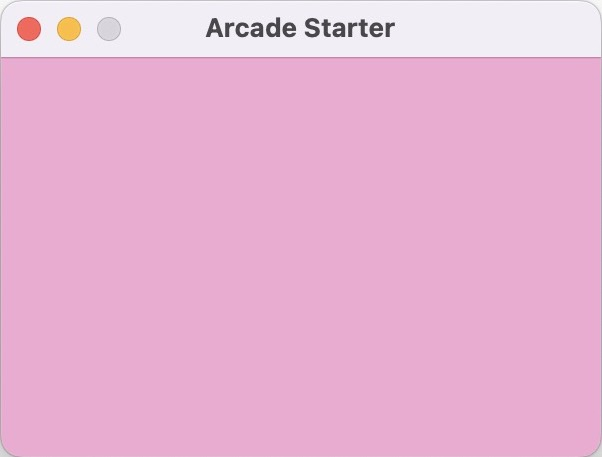
\includegraphics[width=.4\linewidth]{images/ch07/starter.jpg}};
    \drawshadow{image}
\end{tikzpicture}
\caption{}
\label{fig:ch07starter}
\end{figure}

အပေါ်ဆုံးမှာ \fCode{arcade} လိုက်ဘရီ အင်ပို့လုပ်ထားတာပါ။ ရှေ့ပိုင်းမှာသုံးတဲ့ \fCode{from} \fEnEmp{lib} \fCode{import *} ပုံစံ နဲ့ ကွာခြားတာက အခုနည်းနဲ့ အင်ပို့လုပ်ထားရင် လိုက်ဘရီမှာ ပါတဲ့ အစိတ်အပိုင်းတွေကို ဒေါ့ထ်အမှတ်အသားနဲ့ အသုံးပြုရပါမယ်။ ဥပမာ \fCode{open\_window} ဖန်ရှင်ကို
\begin{codetxt}
arcade.open_window(ß\fEnEmp{arguments}ß)
\end{codetxt} 
လိုက်ဘရီ နံမည်နောက်မှာ \fEn{(}\fCodeBf{.}\fEn{)} အမှတ်အသား ခံပြီး ခေါ်ရမှာပါ။ ဒီဖန်ရှင်မှာ လိုချင်တဲ့ဝင်းဒိုး အကျယ်၊ အမြင့်၊ တိုက်တယ်လ်စာသား ထည့်ပေးထားတယ်။ 

\fCode{set\_viewport} ဖန်ရှင်က ဝင်းဒိုးနေရာယူထားတဲ့ စခရင်ဧရီယာမှာ ကိုဩဒိနိတ်စစ်စတမ် သတ်မှတ်ပေးတာပါ။ \fEn{Origin} အမှတ်နဲ့  $x, y$ ဒါရိုက်ရှင် သတ်မှတ်ပေးတာပါ။
%
\begin{py}
arcade.set_viewport(left=0, right=300, top=0, bottom=200)
\end{py}
%
ဝင်းဒိုး ဘယ်ဘက်စွန်းကို $x = 0,$ ညာဘက်စွန်းကို $x = 300$ သတ်မှတ်ထားတယ်။ အပေါ်ဘက်စွန်း (တိုက်တယ်လ်ဘားမပါ) ကို $y = 0,$ အောက်ဘက်စွန်းကို $y = 200$ သတ်မှတ်ထားပါတယ်။ ဝင်းဒိုးရဲ့ ဘယ်ဘက်အပေါ်ထောင့်စွန်းက \fEn{origin} အမှတ် $(0,0)$ ဖြစ်တယ်။ ဘယ်ဘက်ကို သွားရင် $x$ တန်ဖိုး တိုးသွားပြီး အောက်ဘက်ကို ဆင်းရင် $y$ တန်ဖိုး တိုးသွားမှာဖြစ်တယ်။ အခုလို ကိုယ်တိုင်  မသတ်မှတ်ပေးဘဲ  သူ့နဂိုအရှိအတိုင်းဆိုရင် ‘အောက်ခြေ’ ဘယ်ဘက်စွန်းက \fEn{origin} ဖြစ်နေမှာပါ။ အောက်ခြေကနေ အပေါ်ကိုတက်သွားရင် $y$ တန်ဖိုး များလာမှာပါ။ သူ့နဂိုအတိုင်းက \fCode{set\_viewport} ကို အခုလိုခေါ်ထားတာဖြစ်မယ်။ \fCode{top=200}\fEn{,} \fCode{bottom=0} ပါ။
%
\begin{py}
arcade.set_viewport(left=0, right=300, top=200, bottom=0)
\end{py}
%
အသုံးများတဲ့ ဂိမ်းလိုက်ဘရီတွေမှာ ဒီစနစ်ကို သုံးကြတာ မတွေ့ရဘူး။ ဒီစနစ်နဲ့ အကျင့်ဖြစ်သွားရင် အခြားလိုက်ဘရီတွေ လေ့လာတဲ့အခါ အခက်အခဲရှိနိုင်တယ်။ အခုလေ့လာကြမဲ့ ဥပမာတွေ အတွက်လည်း အပေါ်မှာပြောတဲ့နည်းက ပိုအဆင်ပြေတယ်။ (\fEn{Arcade} ကိုပဲ တစိုက်မတ်မတ်သုံးမယ်၊ လေ့လာမယ်ဆိုရင်တော့ သူ့နဂိုအတိုင်းသုံးတာ အကောင်းဆုံးဖြစ်မှာပါ)။

အောက်ပါ ဖန်ရှင်ကတော့ ဝင်းဒိုးရဲ့ နောက်ခံရောင် သတ်မှတ်တာပါ။ လိုက်ဘရီရဲ့ \fCode{color} မော်ဒျူး \fEn{(\textit{module})} မှာ အရောင်တန်ဖိုးတွေ အဆင်သင့် သတ်မှတ်ပေးထားတယ်။ (မော်ဒျူးဆိုတာ လိုက်ဘရီရဲ့ အစိတ်အပိုင်းတစ်ခုလို့ အကြမ်းဖျဉ်း ယူဆနိုင်တယ်)။ 
%
\begin{py}
arcade.set_background_color(arcade.color.PINK_PEARL)
\end{py}
%
အခုလို အင်ပို့လုပ်ထားရင် အရောင်တွေ သုံးရတာ ပိုအဆင်ပြေတယ်
%
\begin{py}
import arcade
from arcade.color import *
ß$\ldots$ß
arcade.set_background_color(PINK_PEARL)
\end{py}
%
\fCode{PINK\_PEARL}\fEn{,} \fCode{RED} စသည်ဖြင့် အရောင်နံမည် တမ်းရေးလို့ရတယ်။ ရှေ့မှာ \fCode{arcade.color.} ထည့်ဖို့  မလိုတော့ဘူး။

ပုံဆွဲဖို့ အဆင်သင့်ဖြစ်အောင် \fCode{start\_render} ခေါ်ပေးရမယ်။ ဆွဲပြီးရင်လည်း \fCode{finish\_render} ခေါ်ဖို့လိုတယ်။ ပုံဆွဲတဲ့ကိစ္စကို ၎င်းတို့နှစ်ခုကြားမှာ  လုပ်ရမှာပါ။
%
\begin{py}
arcade.start_render()
# call drawing functions here
ß$\ldots$ß
ß$\ldots$ß
arcade.finish_render()
\end{py}
%
\betweenminted{\medskipamount}
%
\begin{py}
arcade.run()
\end{py}
%
ဝင်းဒိုးကို မပိတ်မချင်း ပေါ်နေအောင် \fCode{run} ဖန်ရှင် ခေါ်ပေးရတာပါ။ မခေါ်ထားဘဲ ပရိုဂရမ်ကို \fEn{run} ရင် ဝင်းဒိုးပွင့်လာပြီး ဖျတ်ခနဲ ပြန်ပိတ်သွားမှာပါ။ မကျန်ခဲ့ဖို့ သတိပြုရပါမယ်။

\fEn{Arcade} မှာ ပါတဲ့ အခြေခံ ပုံဆွဲဖန်ရှင် တချို့ကို ဆက်ကြည့်ရအောင်။ ထောင့်မှန်စတုဂံဆွဲတဲ့ ဖန်ရှင်တွေထဲက နှစ်ခု သုံးပြထားတယ်။ နှစ်ခုလုံးက  ထောင့်မှန်စတုဂံရဲ့ ဘယ်ဘက်အပေါ်ထောင့်စွန်းနဲ့ တည်နေရာကို သတ်မှတ်ပြီး အရွယ်အစားကို အကျယ်၊ အမြင့်နဲ့ သတ်မှတ်ပေးရတာပါ။  \fCode{draw\_xywh\_rec\allowbreak tangle\_filled} က အတွင်းပိုင်း အရောင်နဲ့ ဆွဲပေးတယ်။ အနားတွေကိုပဲ ဆွဲချင်ရင် \fCode{draw\_xywh\_rec\allowbreak tangle\_outline} ဖန်ရှင်သုံးရပါမယ်။
%
\begin{py}
import arcade
from arcade.color import *

arcade.open_window(300, 200, "Drawing Example")
arcade.set_viewport(0,300, 200, 0)

arcade.set_background_color(PINK_PEARL)
arcade.start_render()
# start drawing
arcade.draw_xywh_rectangle_filled(5,5,200, 50,BABY_BLUE)
arcade.draw_xywh_rectangle_outline(5,5,200, 50,BLACK)

arcade.draw_xywh_rectangle_filled(5,55,200, 50,PALE_VIOLET_RED)
arcade.draw_xywh_rectangle_outline(5,55,200, 50,BLACK)
#finish drawing
arcade.finish_render()
arcade.run()
\end{py}
%
အပေါ် ထောင့်မှန်စတုဂံပုံကို ဒီနှစ်ခုနဲ့ 
%
\begin{py}
arcade.draw_xywh_rectangle_filled(5,5,200, 50,BABY_BLUE)
arcade.draw_xywh_rectangle_outline(5,5,200, 50,BLACK)
\end{py}
%
ဆွဲထားတာပါ $\big\llbracket$ပုံ (\fRefNo{\ref{fig:ch07rects}})$\big\rrbracket$။ ပါရာမီတာတွေက $x, y, width, height, color$ အစဉ်အတိုင်းပဲ။ ဘယ်ဘက်ဘောင်ကနေ $x = 5$ ယူနစ် ခွာထားတယ်။  အပေါ်ဘောင်ကနေလည်း $y = 5$ ယူနစ်ခွာထားတယ်။ သုညထားပြီး စမ်းကြည့်ပါ။ အခြားတန်ဖိုးတွေ ထည့်ပြီး စမ်းကြည့်ပါ။ ပိုပြီးသဘောပေါက် လာပါလိမ့်မယ်။ ဒုတိယ ထောင့်မှန်စတုဂံက ဒီနှစ်ခုနဲ့
%
\begin{py}
arcade.draw_xywh_rectangle_filled(5,55,200, 50,PALE_VIOLET_RED)
arcade.draw_xywh_rectangle_outline(5,55,200, 50,BLACK)
\end{py}
%
ဆွဲထားတာပါ။ ဘယ်ဘက်ကို ခွာထားတာက အပေါ်ပုံနဲ့ တူတူပဲ $(x = 5)$။ အပေါ်ပုံရဲ့ အောက်ခြေအနားနဲ့ ကပ်နေအောင် $y = 5 + 50 (height) = 55$ ထားရပါမယ်။
\begin{figure}[tb!]
\begin{tikzpicture}
    \node[anchor=south west,inner sep=0] (image) at (0,0)
        {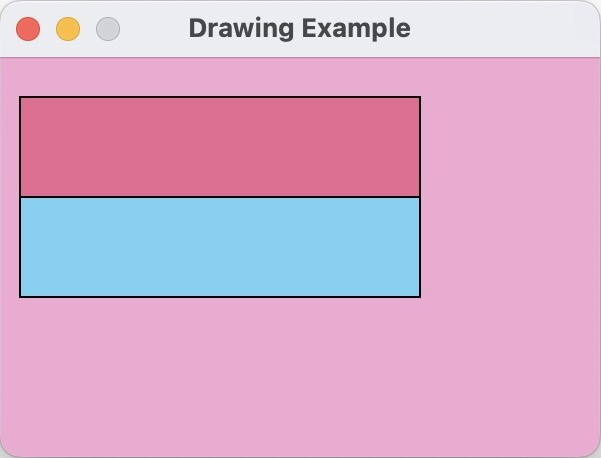
\includegraphics[width=.4\linewidth,trim={0mm 0mm 0mm 0.03mm}]{images/ch07/rects.jpg}};
    \drawshadow{image}
\end{tikzpicture}
\caption{}
\label{fig:ch07rects}
\end{figure}

\begin{mytcbox}
\qquad သူ့နဂိုအတိုင်းဆိုရင် \fEn{Arcade} ကိုဩဒိနိတ်စနစ်မှာ \fEn{origin} က  အောက်ခြေဘယ်ဘက်စွန်းလို့ ပြောခဲ့ပါတယ်။  \fCode{set\_viewport} နဲ့ အပေါ်ဘယ်ဘက်စွန်းကို \fEn{origin} အဖြစ်ပြောင်းလဲ သတ်မှတ်ထားတယ်။ ဒီ့အတွက်ကြောင့် အထက်အောက် ပြောင်းပြန်ဖြစ်သွားပါတယ်။ ဖန်ရှင် \fEn{documentation} မှာကြည့်ရင် အခုလိုတွေ့ရမှာပါ (\fEn{VS Code/PyCharm} မှာ  မောက်စ်ပွိုင်တာကို ဖန်ရှင်နံမည်ပေါ်မှာထားရင် \fEn{documentation} ပြပေးပါလိမ့်မယ်)
%
\begin{pytc}
def draw_xywh_rectangle_filled(bottom_left_x: float,
                               bottom_left_y: float,
                               width: float,
                               height: float,
                               color: tuple[int, int, int] 
                                   | list[int] 
                                   | tuple[int, int, int, int]) -> None
\end{pytc}
%
\fEn{Documentation} မှာ \fEn{bottom} ဆိုရင် ကိုယ့်အတွက် \fEn{top} လို့ ပြောင်းပြန် စဉ်းစားရမယ်။ သူ့နဂိုစနစ်ကို ပြောင်းလိုက်လို့ ဒီအခက်အခဲ ကြုံရတာပါ။ ဒါကြောင့် \fEn{Arcade} ကိုပဲ အဓိကသုံးမယ်ဆိုရင် သူ့အရှိအတိုင်းသုံးတာ အကောင်းဆုံးပဲ။ အထက်အောက် ပြောင်းပြန် စဉ်းစားစရာ မလိုတော့ဘူး။
\end{mytcbox}






\label{lst:checkerboard}
%
\begin{py}
import arcade
from arcade.color import *

WIN_WIDTH = 600
BOARD_SIZE = 400
WIN_HEIGHT = 420
arcade.open_window(WIN_WIDTH, WIN_HEIGHT, "Arcade Checkerboard")
arcade.set_viewport(left=0,
                    right=WIN_WIDTH,
                    top=0,
                    bottom=WIN_HEIGHT)
arcade.set_background_color(WHITE_SMOKE)
arcade.start_render()

COLS = 8
ROWS = 8
SQ_SIZE = BOARD_SIZE / ROWS
X_LFT = (WIN_WIDTH - BOARD_SIZE) / 2
Y_TOP = (WIN_HEIGHT - BOARD_SIZE) / 2 + 1

for i in range(ROWS):
    for j in range(COLS):
        x = X_LFT + SQ_SIZE * i
        y = Y_TOP + SQ_SIZE * j
        if (i + j) % 2 == 0:
            arcade.draw_xywh_rectangle_filled(x,
                                              y,
                                              SQ_SIZE,
                                              SQ_SIZE,
                                              WOOD_BROWN)
        else:
            arcade.draw_xywh_rectangle_filled(x,
                                              y,
                                              SQ_SIZE,
                                              SQ_SIZE,
                                              BLACK)
        arcade.draw_xywh_rectangle_outline(x,
                                           y,
                                           SQ_SIZE,
                                           SQ_SIZE,
                                           BLACK)

arcade.finish_render()
arcade.run()
\end{py}
%

\begin{figure}[tb!]
\begin{tikzpicture}
    \node[anchor=south west,inner sep=0] (image) at (0,0)
        {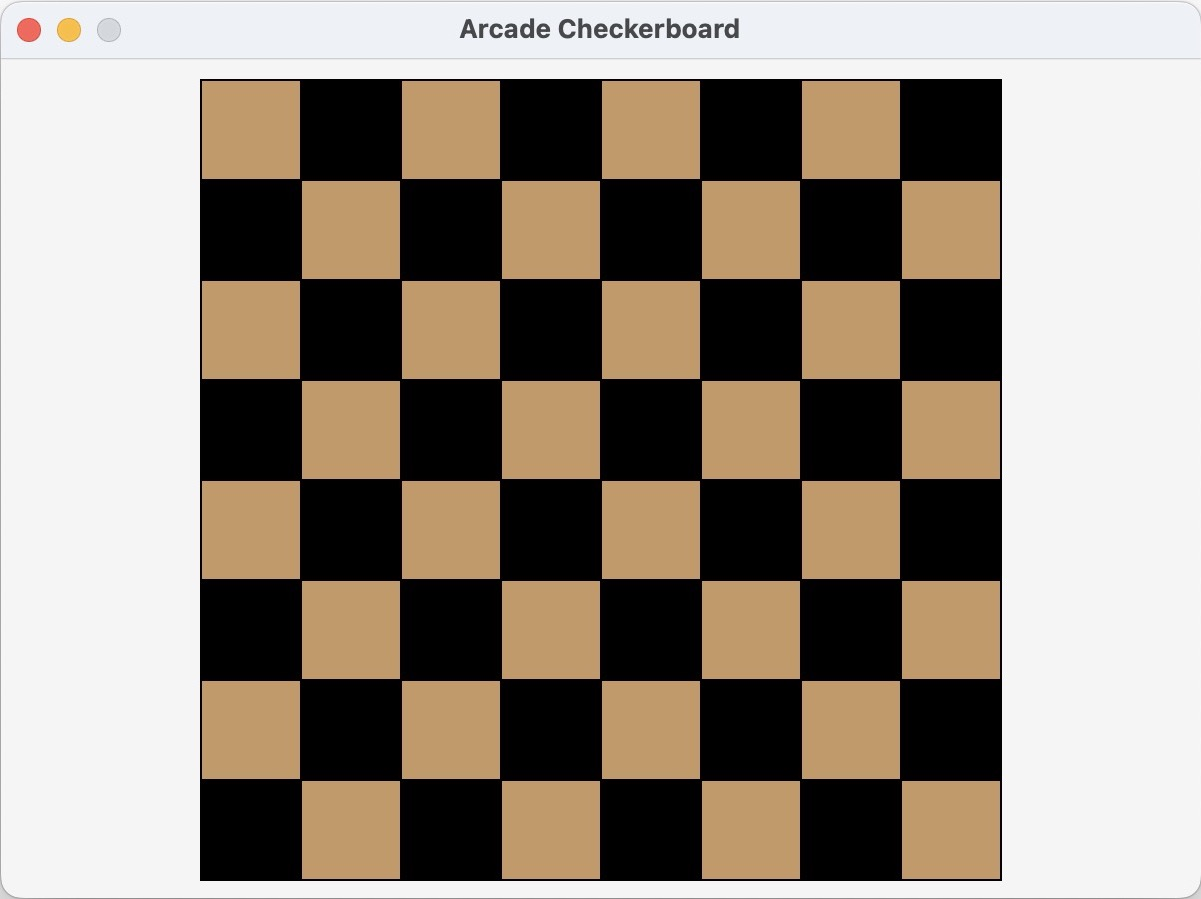
\includegraphics[width=.85\linewidth]{images/ch07/checkerboard.jpg}};
    \drawshadow{image}
\end{tikzpicture}
\caption{}
\label{fig:ch07chkbrd}
\end{figure}

\section{\fSecCodeBf{while} loop}
\fCode{while} \fEn{loop} ဟာ \fEnEmp{indefinite loop} ဖြစ်ပါတယ်။ \fEn{Loop} ကို စတင် လုပ်ဆောင်တဲ့အချိန်မှာ ဘယ်နှစ်ကြိမ် ပြန်ကျော့မလဲ အတိအကျ ကြို ‘မသိ’ ရင်  \fEn{indefinite loop} လို့ သတ်မှတ်တယ်။ တစ်နဲ့ တစ်ဆယ်ကြား (အပါအဝင်) ကိန်းပြည့်တစ်လုံးကို ကျပန်း \fEn{(random)} ထုတ်ထားမယ်။ မမှန်မချင်း အဲဒီဂဏန်းကို ခန့်မှန်းပေးရမယ်။ ခန့်မှန်းတာ မှန်သွားရင် ဘယ်နှစ်ခါ ခန့်မှန်းရလဲနဲ့ မှန်တဲ့ဂဏန်းကို ပြပေးတဲ့ ပရိုဂရမ်မှာ \fCode{while} \fEn{loop} အသုံးပြု ရေးထားတာ တွေ့ရပါမယ်။

%
\begin{py}
from random import *

num = randint(1, 10)

guess = int(input('? '))
times = 1
while guess != num:
    guess = int(input('? '))
    times += 1

print(f'You get correctly after {times} guesses.')
print(f'The number is {num}.')
\end{py}
%

\fCode{guess != num} (ဘူလီယန် အိပ်စ်ပရက်ရှင်) မမှားမချင်း \fEn{loop} က ပြန်ကျော့ပေးနေမှာပါ။ မှားတဲ့အခါ ထပ်မကျော့တော့ဘဲ ရပ်သွားမှာဖြစ်တယ်။ ကျပန်းဂဏန်းက ခုနှစ်ကျတယ် ဆိုပါစို့။ တစ်၊ ကိုး၊ သုံး၊ တစ်ဆယ်နဲ့ ခုနှစ် တို့ကို အစဉ်အတိုင်း ခန့်မှန်း ထည့်ပေးမယ်ဆိုရင် တစ်ကျော့ချင်း လိုက်ကြည့်တဲ့အခါ အခုလို တွေ့ရမှာပါ။

%
\begin{py}
num = randint(1, 10)            #ß 7 \fMM{ကျတယ် ယူဆပါ}ß

guess = int(input('? '))        #ß 1 \fMM{ထည့်ပေးတယ်}ß
times = 1

guess != num:                   #ß 1 != 7 \fMM{က \fCode{True}}ß
    ß\fEnBf{1\textsuperscript{\fEnBf{st}} iter:}ß
    guess = int(input('? '))    #ß 9 \fMM{ထည့်ပေးတယ် ယူဆပါ}ß
    times += 1                  #ß 2 \fMM{ဖြစ်သွားမယ်}ß

guess != num:                   #ß 9 != 7 \fMM{က \fCode{True}}ß
    ß\fEnBf{2\textsuperscript{\fEnBf{nd}} iter:}ß
    guess = int(input('? '))    #ß 3 \fMM{ထည့်ပေးတယ် ယူဆပါ}ß
    times += 1                  #ß 3 \fMM{ဖြစ်သွားမယ်}ß

guess != num:                   #ß 10 != 7 \fMM{က \fCode{True}}ß
    ß\fEnBf{3\textsuperscript{\fEnBf{rd}} iter:}ß
    guess = int(input('? '))    #ß 10 \fMM{ထည့်ပေးတယ် ယူဆပါ}ß
    times += 1                  #ß 4 \fMM{ဖြစ်သွားမယ်}ß

guess != num:                   #ß 7 != 7 \fMM{က \fCode{False} ဖြစ်သွားပြီ}ß
    #ß \fMM{ထပ်မကျော့တော့ဘူး}ß

#ß \fMM{\fEn{loop} အောက်က စတိတ်မန့်တွေ ဆက်လုပ်ပါတယ်}ß
print(f'You get correctly after {times} guesses.')
print(f'The number is {num}.')  
\end{py}
%

\fEn{Loop} က ထပ်မကျော့တော့ဘဲ  ရပ်သွားတာကို  \fEn{\textit{loop exits}} ဖြစ်သွားတယ်လို့ ပြောတယ်။ မြန်မာလိုတော့ \fEn{loop} ကနေ ထွက်သွားတယ်ပေါ့။ အကယ်၍ စောစောက ဥပမာမှာ ပထမဆုံးတစ်ခါမှာပဲ ခုနှစ် ထည့်လိုက်ရင်တော့ ဘလောက်ကို တစ်ခါမှ မလုပ်ဆောင်ဘဲ \fEn{loop} က ချက်ချင်းထွက်သွားမှာပါ။

\subsection*{Sentinel Controlled Loop}
ဂဏန်းတွေ ဘယ်နှစ်လုံး ပေါင်းမှာလဲ ကြိုသိရင် \fCode{for} \fEn{loop} နဲ့ အလုပ်ဖြစ်တယ်။ ဂဏန်း ဘယ်နှစ်လုံးရှိလဲ ကြိုမသိထားဘဲ ရှိသလောက် တစ်လုံးချင်းရိုက်ထည့်ပြီး အားလုံးပေါင်းချင်တာဆိုရင်တော့ \fCode{for} \fEn{loop} နဲ့ အဆင်မပြေဘူး (မရနိုင်ဘူးလို့ မဆိုလိုပါ၊ မရမက လုပ်တဲ့နည်းတွေလည်း ရှိပါတယ်)။ ဒီလိုအခြေအနေမျိုးမှာ \fEnEmp{sentinel controlled loop} ကို သုံးပါတယ်။ 

\fEn{Sentinel controlled loop} မှာ \fEn{loop} ကနေ ထွက်ဖို့အတွက် အသုံးပြုတဲ့ သီးသန့်တန်ဖိုးတစ်ခု ရှိရပါမယ်။ ဒီတန်ဖိုးကို \fEnEmp{sentinel value} လို့ ခေါ်တယ်။ ဂဏန်းတွေပေါင်းတဲ့ ကိစ္စအတွက်  \fEnEmp{sentinel value} ရွေးချယ်သတ်မှတ်တဲ့အခါ ပေါင်းရမဲ့ဂဏန်း မဖြစ်နိုင်တဲ့ တစ်ခုကို ရွေးရပါမယ်။ သုညဟာ ‌အပေါင်းထပ်တူရ ဂုဏ်သတ္တိရှိတဲ့အတွက် ၎င်းကို \fEnEmp{sentinel value} အဖြစ် ထားနိုင်တယ်။
%
\begin{py}
# File: add_nums_sentinel.py 
SENTINEL = 0
total = 0

val = int(input('? '))
while val != SENTINEL:
    total += val
    val = int(input('? '))

print(f'Total is {total}')
\end{py}
%
ထည့်ပေးတဲ့ ဂဏန်းဟာ သုညမဟုတ်မချင်း \fCode{total} မှာ ပေါင်းထည့်ပြီး နောက်ဂဏန်းတစ်ခု ထည့်ပေးဖို့ \fEn{input} တောင်းမှာပါ။ \fEn{Sentinel} တန်ဖိုး သုည ထည့်လိုက်ရင် \fEn{loop} က ထွက်သွားမယ်။ ပြီးတဲ့အခါ \fCode{total} ကို ပြပေးမှာပါ။ စစချင်းပဲ သုည ထည့်လိုက်ရင် \fEn{loop} က တစ်ခါမှ မကျော့ဘဲ ထွက်သွားမယ်။ \fCode{total} လည်း သုညပဲ ထွက်ပါမယ်။ အခုပရိုဂရမ်ကို နောက်တစ်နည်း ရေးလို့ရပါတယ်။ 
%
\begin{py}
# File: add_nums_sentinel2.py 
SENTINEL = 0
total = 0

while True:
    val = int(input('? '))
    if val == SENTINEL:
        break
    total += val

print(f'Total is {total}')

\end{py}
%

\fCode{while True:} က ပုံမှန်ဆိုရင် \fEn{infinite loop} ဖြစ်ပါလိမ့်မယ်။ အမြဲမှန်နေတဲ့အတွက် ပြန်ကျော့တာ ဘယ်တော့မှ ရပ်မှာ မဟုတ်ဘူး။ ဒီလိုဖြစ်နေတာကို ဖြတ်ချပစ်ဖို့အတွက် \fCode{break} စတိတ်မန့်ကို သုံးထားပါတယ်။ \fCode{if val == SENTINEL:} (ထည့်ပေးတဲ့ တန်ဖိုးက သုညဆိုရင်) လက်ရှိ အလုပ်လုပ်နေတဲ့ \fEn{loop} ကို \fCode{break} လိုက်မှာဖြစ်တယ်။ 

အထက်ပါ \fEn{sentinel loop} ပုံစံနှစ်ခုကို ယှဉ်ကြည့်ရင်  ပထမတစ်ခုမှာ \fEn{input} တန်ဖိုးထည့်ခိုင်းတာကို \fEn{loop} မစမီ တစ်ခါ ကြိုလုပ်ထားရတယ်။ နောက်တစ်ခုမှာတော့ အဲ့ဒီလို ကြိုလုပ်ထားစရာမလိုဘူး။ \fEn{Loop} ဘလောက်ထဲက စတိတ်မန့်တစ်ခုကို အပြင်မှာထုတ်ထားရတဲ့အတွက် တချို့က ပထမပုံစံထက် ဒုတိယပုံစံက ကုဒ်စတိုင်လ်အားဖြင့် ပိုပြီး သပ်ရပ်ကြော့ရှင်းတယ်လို့ ယူဆကြပါတယ်။

\subsection*{Result Controlled Loop}

တစ်နှစ်ငါးရာခိုင်နှုန်း အတိုးနဲ့ ဘဏ်မှာ ဒေါ်လာတစ်ထောင် စုထားတယ်။ တစ်နှစ်ပြည့်တိုင်း အတိုးအရင်း ပေါင်းပြီး နောက်နှစ်အတွက် အတိုးတွက်တယ်။ နှစ်ထပ်တိုး \fEn{(yearly compound interest)} လို့ခေါ်ပါတယ်။ ဒီနည်းလမ်းနဲ့ အနည်းဆုံး ဒေါ်လာတစ်သန်း စုမိဖို့ (မီလျံနာတစ်ယောက်ဖြစ်ဖို့) ဘယ်နှစ်နှစ်စောင့်ရမလဲ။ သုံးနှစ်ပြည့်ရင် စုမိမဲ့ ငွေပမာဏ တွက်ထားတာကို ကြည့်ပါ။


%
\begin{flushleft}
\vspace{1em}
\setlength{\extrarowheight}{3pt}
\begin{tabular}[h]{*{3}l l l}
    \toprule[1.5pt]
        \fTblHead{Year} & \fTblHead{Interest} & \fTblHead{Balance}\\       
    \midrule
    $1$ & $1000 \times 0.05 = 50$ & $1000 + 50 = 1050$\\
    $2$ & $1050 \times 0.05 = 52.5$ & $1050 + 52.5 = 1102.5$\\
    $3$ & $1102.5 \times 0.05 = 55.125$ & $1102.5 + 55.125 = 1157.625$\\   
    \bottomrule[1.5pt]
\end{tabular}
\label{tbl:ch07onem}
\captionof{table}{သုံးနှစ်စာ နှစ်ထပ်တိုး}
\end{flushleft}
%

ဒေါ်လာတစ်သန်း အနည်းဆုံးရဖို့ နှစ်ဘယ်လောက်ကြာမလဲ အခုလို ရှာနိုင်ပါတယ် 


% https://realpython.com/python-f-strings/
%
\begin{py}
# File: one_million.py
balance = 1000
INT_RATE = 0.05
TARGET = 1_000_000
yr = 0

print(f"{'yr':>4s} {'interest':>10s} {'balance':>10s}")
while balance < TARGET:
    interest = balance * INT_RATE
    balance += interest
    yr += 1
    print(f'{yr:4d} {interest:10.2f} {balance:10.2f}')

print(f'You have to wait {yr} years!')
\end{py}
%
\fCode{while} \fEn{loop} ထဲမှာ တစ်နှစ်ကုန်တဲ့အခါ ရမဲ့ အတိုးနဲ့ အတိုးအရင်းပေါင်း တွက်ထားပြီး  \fCode{yr} ကိုလည်း တစ်နှစ် တိုးပေးတယ်။ \fCode{yr}\fEn{,} \fCode{interest}\fEn{,} \fCode{balance} ထုတ်ပြပေးတယ် (မပြလည်း ပြဿနာမရှိပါ၊ တစ်နှစ်စာ တွက်ထားတာ စစ်ကြည့်လို့ရအောင် ထုတ်ကြည့်တာပါ)။ တစ်သန်းမပြည့်မချင်း ပြန်ကျော့ပေးအောင် \fEn{loop} ကွန်ဒီရှင်ကို \fCode{balance < TARGET} နဲ့ စစ်ထားတယ်။ တစ်သန်းနဲ့ညီရင် (သို့) တစ်သန်းကျော်သွားတာနဲ့ ကွန်ဒီရှင် \fCode{False} ဖြစ်သွားပြီး ထပ်မကျော့တော့ဘူး။ \fEn{Loop} တစ်ခါကျော့တိုင်း တစ်နှစ်စာ အတိုးအရင်းပေါင်း \fCode{balance} ကို တွက်ချက်ပြီး \fEn{loop} ကနေ ဘယ်အချိန် ထွက်မလဲကလည်း အဲဒီရလဒ်အပေါ် မူတည်နေတာ တွေ့ရပါမယ်။ ဒီလို သဘောတရားရှိတဲ့ \fEn{loop} မျိုးကို \fEn{result controlled loop} လို့ ခေါ်ပါတယ်။ ကျော့မဲ့ အကြိမ်အရေအတွက်က \fEn{loop} ထဲမှာ တွက်ချက်ထားတဲ့ ရလဒ်ပေါ် မူတည်တယ်။

ပရိုဂရမ် \fEn{output} ကို အခုလို ကော်လံတစ်ခုစီကို အကျယ် တစ်သမတ်တည်းဖြစ်၊ စာသားတွေ ညာဘက်ကပ်ပြီး ညီနေအောင် \fEn{f-strings} ကို \fEn{format spec} လို့ခေါ်တဲ့ ဖော့မတ်သတ်မှတ်တဲ့ နည်းစနစ်ကို သုံးထားတာပါ။
\begin{codetxt}
  yr   interest    balance
   1      50.00    1050.00
   2      52.50    1102.50
 ...      ...      ...    
 142   48602.79 1020658.53
You have to wait 142 years!
\end{codetxt}
\fEn{Format spec} နဲ့ ပါတ်သက်ပြီး အကျယ်တဝင့် မဖော်ပြတော့ဘဲ အခုလို ဖော့မတ်ရအောင် ဘယ်လိုလုပ်ထားလဲကိုပဲ ရှင်းပြပါမယ်။
%
\begin{py}
f"{'yr':>4s} {'interest':>10s} {'balance':>10s}"
\end{py}
%
ကော်လံ ခေါင်းစည်း အတွက် \fEn{f-string} ပါ။ ဖော့မတ်လုပ်ရမဲ့ တန်ဖိုး/ဗေရီရေဘဲလ်/အိပ်စ်ပရက်ရှင်က \fCode{:} (ကော်လံ) ဘယ်ဘက်မှာ ရှိမယ်။ ညာဘက်မှာ  \fEn{format spec} ရှိမယ်။ \fCodeBf{>4s} က \fCode{'yr'} အတွက် \fEn{format spec} ဖြစ်တယ်။ \fCodeBf{>} က ညာဘက်ကပ်ဖို့၊ \fCodeBf{4} က ကော်လံအကျယ်ကို ကာရက်တာ လေးလုံးသတ်မှတ်တာ။ \fCodeBf{s} ကတော့ တန်ဖိုးကို \fEn{string} အနေနဲ့ ပြပေးပါလို ဆိုလိုတယ်။ ကျန်တဲ့ ကော်လံနှစ်ခု အတွက် \fEn{format spec} ကို \fCodeBf{>10s} သတ်မှတ်တယ်။  ကာရက်တာ ဆယ်လုံး ကော်လံအကျယ် သတ်မှတ်တယ်။
%
\begin{py}
f'{yr:4d} {interest:10.2f} {balance:10.2f}'
\end{py}
%
ဒါကတော့ \fCode{yr}\fEn{,} \fCode{interest}\fEn{,} \fCode{balance} တန်ဖိုးတွေကို ပြပေးဖို့ပါ။ ကော်လံအကျယ် \fCode{4}\fEn{,} \fCode{10}\fEn{,} \fCode{10} သတ်မှတ်တယ်။ \fCode{yr} ကို ကိန်းပြည်ဂဏန်းအနေနဲ့ ပြပေးအောင် \fCode{d} သုံးတယ်။ ကျန်တဲ့နှစ်ခုကို ဒဿမနဲ့ ပြဖို့ \fCode{f} သုံးတယ်။ \fCode{.2} ကတော့ ဒဿမနောက် ဂဏန်းနှစ်လုံး ပြပေးခိုင်းတာ။ ကိန်းဂဏန်းဆိုရင် သူ့နဂိုအတိုင်း ညာဘက်ကပ်ပေးတဲ့အတွက် \fCode{>} ထည့်ဖို့ မလိုဘူး။ ဘယ်ဘက်ကပ်ချင်ရင် \fCode{<} သုံးလို့ရတယ်။

\section{လေ့ကျင့်ရန် ဥပမာများ}

ကွန်ထရိုးလ် စထရက်ချာတွေ အသုံးချတတ်လာအောင် များများလေ့ကျင့်၊ များများစဉ်းစား၊ များများရေးကြည့် ရမှာပါ။ ဘယ်အတတ်ပညာမဆို များများလေ့ကျင့်မှ ကျွမ်းကျင်လာနိုင်မှာပါ။ ဒီသဘောအရ ပရိုဂရမ်းမင်း ပညာရပ်ဟာလည်း ချွင်းချက်မဖြစ်နိုင်ပါဘူး။

\begin{mytcbox}
အောက်ပါ ဥပမာတစ်ခုချင်းကို ပုစ္ဆာနားလည်အောင်ဖတ်ပြီး ကိုယ်တိုင်စဉ်းစား ရေးကြည့်ဖို့ လေးလေးနက်နက် အကြံပြုပါတယ်။ ရေးပြီးသွားရင် ပုစ္ဆာမှာ ဖော်ပြထားချက်နဲ့ အညီ အလုပ်လုပ်/မလုပ် ဟာကွက်မရှိအောင် ဘယ်လိုစစ်ဆေး စိစစ်မလဲ မိမိဘာသာ စဉ်းစားကြည့်ပါ။
\end{mytcbox}

\subsection*{Internet Delicatessen}
\fEn{Online} ကနေ အစားအသောက်တွေ \fEn{delivery} ပို့ပေးဖို့ အမှာလက်ခံတဲ့ ဆိုင်လေးတစ်ဆိုင်အတွက် ပရိုဂရမ်ရေးပေးရပါမယ်။ အော်ဒါမှာတဲ့အခါ မှာမဲ့ အစားအသောက် နံမည်၊ ဈေးနှုန်းနဲ့ အိပ်စ်ပရက်စ် \fEn{delivery} ယူမယူ ပရိုဂရမ်မှာ ထည့်ပေးရပါမယ်။ ပရိုဂရမ်က အော်ဒါနဲ့ စုစုပေါင်းကျသင့်ငွေကို ထုတ်ပေးရပါမယ်။ တစ်သောင်းနဲ့အထက်မှာရင် \fEn{delivery} ဖိုး ပေးစရာမလိုပါ။ တစ်သောင်းအောက်ဆိုရင်တော့ နှစ်ရာပေးရပါမယ်။ အိပ်စ်ပရက်စ် \fEn{delivery} ယူမယ်ဆိုရင် သုံးရာအပို ထပ်ပေးရပါမယ်။
%
\begin{minted}[frame=lines, framerule=0pt,escapeinside=ßß]{text}
ß\fEn{Enter the item: Tuna Salad}ß
ß\fEn{Enter the price: 4500}ß
ß\fEn{Express delivery (0==no, 1==yes): 1}ß

ß\fEn{Invoice:}ß
ß\fEn{Tuna Salad\space\space 4500}ß
ß\fEn{delivery\space\space\space\space\space\space\space 500}ß 
ß\fEn{total\space\space\space\space\space\space\space\space\space\space\space 5000}ß
\end{minted}
%

%
\begin{py}
itm_name = input('Item name: ')
price = int(input('Price: '))
is_exp_deli = int(input('Express delivery (0==no, 1==yes): '))

tot_deli_fee = 0
if price >= 10_000 and is_exp_deli == 1:
    tot_deli_fee = 300
elif price >= 10_000 and is_exp_deli == 0:
    tot_deli_fee = 0
elif price < 10_000 and is_exp_deli == 1:
    tot_deli_fee = 200 + 300
elif price < 10_000 and is_exp_deli == 0:
    tot_deli_fee = 200
else:
    print("You may have wrong value for express deli.")

tot_cost = price + tot_deli_fee

print("Invoice: ")
print(f'{itm_name:<10s} {price:8.2f}')
print(f"{'delivery':<10s} {tot_deli_fee:8.2f}")
print(f"{'total':<10s} {tot_cost:8.2f}")
\end{py}
အိပ်စ်ပရက်စ် \fEn{delivery} ယူ/မယူ တစ် (သို့) သုည ထည့်ပေးရမှာပါ။ တစ်/သုည မဟုတ်တဲ့ ဂဏန်းတစ်ခု မှားထည့်မိရင် \fCode{if...elif} ကွန်ဒီရှင်တွေ တစ်ခုမှ \fCode{True} ဖြစ်မှာ မဟုတ်ပါဘူး။ မှားထည့်ထားတယ်လို့ သတိပေးဖို့ \fCode{else} အပိုင်းမှာ လုပ်ထားတယ်။ မှန်/မမှန် စိစစ်တဲ့အခါ အောက်ပါဇယားမှ ဖြစ်နိုင်ခြေအားလုံး ခြုံငုံမိအောင် စစ်သင့်တယ်။ အိပ်စ်ပရက်စ် \fEn{delivery} အတွက် \fEn{input} ဂဏန်း မှားထည့်ရင် သတိပေးတာကိုလည်း စစ်သင့်တယ်။ တစ်သောင်းဖိုး ဝယ်တာကို သုံးမျိုးစစ်ထားတာ လေ့လာကြည့်ပါ။ တစ်သောင်း မပြည့်တာနဲ့ တစ်သောင်းကျော်ဖိုး အတွက်လည်း အလားတူ စစ်ကြည့်လို့ အားလုံးမှန်တယ်ဆိုရင် ဒီပရိုဂရမ်မှာ \fEn{bug} ပါနိုင်ခြေ လုံးဝမရှိသလာက် ဖြစ်သွားပါပြီ။ 

%
\begin{flushleft}
\vspace{1em}
\setlength{\extrarowheight}{3pt}
\begin{tabular}[h]{*{3}l l l}
    \toprule[1.5pt]
        \fTblHead{10,000 MMK and above?} & \fTblHead{Express Delivery?}\\       
    \midrule
    \fEn{Yes} & \fEn{Yes}  \\
    \fEn{Yes} & \fEn{No}   \\
    \fEn{No}  & \fEn{Yes}  \\
    \fEn{No}  & \fEn{No}   \\
       
    \bottomrule[1.5pt]
\end{tabular}
\label{tbl:ch07inetdeli}
\captionof{table}{သုံးနှစ်စာ နှစ်ထပ်တိုး}
\end{flushleft}
%
\vspace*{1em}
\noindent\fEn{Test Output:}
\begin{codetxt}
Item name: Salad
Price: 10000
Express delivery (0==no, 1==yes): 1
Invoice: 
Salad      10000.00
delivery     300.00
total      10300.00
\end{codetxt}
\betweenminted{\medskipamount}
\begin{codetxt}
Item name: Salad
Price: 10000
Express delivery (0==no, 1==yes): 0
Invoice: 
Salad      10000.00
delivery       0.00
total      10000.00
\end{codetxt}
\betweenminted{\medskipamount}
\begin{codetxt}
Item name: Salad
Price: 10000
Express delivery (0==no, 1==yes): 2
You may have wrong value for express deli.
Invoice: 
Salad      10000.00
delivery       0.00
total      10000.00
\end{codetxt}

ပရိုဂရမ်တစ်ခုရဲ့ လိုအပ်ချက်ဟာ မကြာခဏ ပြောင်းလဲသွားလေ့ရှိတယ်။ အခုပရိုဂရမ်မှာ ‌ဈေးနှုန်းသတ်မှတ်ချက်တွေ ပြောင်းလဲနိုင်တယ်။ အနည်းဆုံး တစ်သောင်းခွဲဝယ်မှ ပို့ခ \fEn{free} ရမှာဖြစ်ပြီး တစ်သောင်းခွဲအောက်ဆိုရင် ပို့ခ သုံးရာ့ငါးဆယ် ပြောင်းလဲသတ်မှတ်လိုက်တဲ့အပြင် အိပ်စ်ပရက်စ် \fEn{delivery} ကလည်း တစ်ရာဈေးထပ်တက်သွားတယ် ဆိုပါစို့။ တကယ့်လက်တွေ့မှာလည်း ဒါမျိုးဖြစ်လေ့ရှိပါတယ်။ ဒီအတွက်ကို ပရိုဂရမ်ကို ပြင်ပေးရပါမယ်။ ဆိုင်ပိုင်ရှင်ကလည်း ဈေးနှုန်းမကြာခဏ ပြောင်းဖို့လိုနိုင်ကြောင်း ပြောလာပါတယ်။ နောင်လည်း ထပ်ပြင်ပေးဖို့လိုမဲ့ သဘောပါ။ လွယ်လွယ်ကူကူ ပြင်ပေးနိုင်ရင် အကောင်းဆုံးပါ။ ပြင်ဆင်တဲ့အခါ မှားနိုင်ခြေနည်းဖို့လည်း အရေးကြီးပါတယ်။ ခုရေးထားတဲ့အတိုင်းဆိုရင် ပြီးခဲ့တဲ့ပရိုဂရမ်မှာ ပြဿနာရှိနေပါတယ်။

ပြီးခဲ့တဲ့ ပရိုဂရမ်မှာ ပြင်မယ်ဆိုရင် \fCode{10\_000} ကို လေးနေရာ၊ ပုံမှန်ပို့ခ \fCode{200} နဲ့ အိပ်စ်ပရက်စ်အပိုကြေး \fCode{300} စတာတွေကို နှစ်နေရာစီ လိုက်ပြင်ရပါမယ်။ အလုပ်ရှုပ်တဲ့အပြင် ပြင်ဖို့ကျန်ခဲ့တာလို့  မှားတာလည်း ဖြစ်နိုင်တယ်။ \fEn{“Find and Replace”} လုပ်မှာပေါ့လို့ စောဒကတက်စရာ ရှိပါတယ်။ အခုလို ကုဒ်လိုင်း နည်းနည်းပဲရှိတဲ့ ပရိုဂရမ်အသေးလေးမှာ အဆင်ပြေနိုင်ပေမဲ့ ပိုရှုပ်ထွေးပြီး ကုဒ်လိုင်းတွေများတဲ့ ပရိုဂရမ်မျိုးတွေမှာ \fEn{“Find and Replace”} လုပ်ရင် မပြင်သင့်တာတွေကိုပါ မရည်ရွယ်ပဲ ပြင်မိသွားတာဖြစ်တတ်ပါတယ်။ ပရိုဂရမ်ရေးတဲ့အခါ ကျင့်သုံးရမဲ့ အလေ့အထကောင်းတစ်ခုက ကုဒ်ထဲမှာ ဒီတိုင်းချရေးထားတဲ့ တန်ဖိုးတွေ \fEn{(literal constants)} တွေကို နာမည်ပေးထားတာပါ။ အပေါ်က ပရိုဂရမ်မှာ \fEn{literal constants} တွေချည်း သုံးထားတယ်။ နံမည်ပေးထားတဲ့ \fEn{constants} \fEn{(named constants)} တွေအဖြစ် ပြောင်းရေးသင့်တယ်။
%
\begin{py}
FREE_DELI_AMT = 15_000
DELI_FEE = 350
EXP_DELI_FEE = 400

itm_name = input('Item name: ')
price = int(input('Price: '))
is_exp_deli = int(input('Express delivery (0==no, 1==yes): '))

tot_deli_fee = 0

if price >= FREE_DELI_AMT and is_exp_deli == 1:
    tot_deli_fee = EXP_DELI_FEE
elif price >= FREE_DELI_AMT and is_exp_deli == 0:
    tot_deli_fee = 0
elif price < FREE_DELI_AMT and is_exp_deli == 1:
    tot_deli_fee = DELI_FEE + EXP_DELI_FEE
elif price < FREE_DELI_AMT and is_exp_deli == 0:
    tot_deli_fee = DELI_FEE
else:
    print("You may have wrong value for express deli.")

tot_cost = price + tot_deli_fee
print("Invoice: ")
print(f'%-10s %8.2f' % (itm_name, price))
print(f'%-10s %8.2f' % ('delivery', tot_deli_fee))
print(f'%-10s %8.2f' % ('total', tot_cost))
\end{py}
%

ဒီပရိုဂရမ်ကို \fEn{cascading} \fCode{if} မသုံးဘဲ ရိုးရိုး \fCode{if} နဲ့ ရေးလို့လည်း ရတယ်။ 
%
\begin{py}
FREE_DELI_AMT = 15_000
DELI_FEE = 350
EXP_DELI_FEE = 400

itm_name = input('Item name: ')
price = int(input('Price: '))
is_exp_deli = int(input('Express delivery (0==no, 1==yes): '))

tot_deli_fee = 0

if price < FREE_DELI_AMT:
    tot_deli_fee += DELI_FEE

if is_exp_deli == 1:
    tot_deli_fee += EXP_DELI_FEE

if not (is_exp_deli == 0 or is_exp_deli == 1):
    print("You may have wrong value for express deli.")

tot_cost = price + tot_deli_fee

print("Invoice: ")
print(f'%-10s %8.2f' % (itm_name, price))
print(f'%-10s %8.2f' % ('delivery', tot_deli_fee))
print(f'%-10s %8.2f' % ('total', tot_cost))
\end{py}
%
ပထမ \fCode{if} က \fEn{delivery} ခ ပေးဖို့ လိုတယ်ဆိုရင် \fCode{tot\_deli\_fee} မှာ \fCode{DELI\_FEE} ပေါင်းထည့်ပေးတယ်။ ဒုတိယ \fCode{if} က အိပ်စ်ပရက်စ် \fEn{delivery} ယူမယ်ဆိုရင် \fCode{tot\_deli\_fee} မှာ \fCode{EXP\_DELI\_FEE} ထပ်ပေါင်းထည့်တယ်။ အောက်ဆုံး \fCode{if} ကတော့ အိပ်စ်ပရက်စ် \fEn{delivery} အတွက် တစ်နဲ့ သုည မဟုတ်တာ ထည့်မိရင် သတိပေးစာသား ပြပေးတယ်။

ဒီပရိုဂရမ်နဲ့ ဒီ့မတိုင်ခင် သူ့ရှေ့က ပရိုဂရမ်က ဖြစ်နိုင်ခြေအားလုံးအတွက်တော့ ရလဒ် တူတူမထွက်ပါဘူး။  အခြေအနေ တစ်ခုကလွဲလို့ ကျန်တာတွေအတွက်တော့ ရလဒ်တူပါတယ်။ တစ်သောင်းငါးထောင် ထက်ငယ်တဲ့ တန်ဖိုးနဲ့ အိပ်စ်ပရက်စ် \fEn{delivery} အတွက် ဂဏန်း လွဲထည့်ကြည့်ပါ။ ဥပမာ

\begin{codetxt}
Item name: salad
Price: 12000
Express delivery (0==no, 1==yes): 2
You may have wrong value for express deli.
Invoice: 
salad      12000.00
delivery       0.00
total      12000.00
\end{codetxt}
\betweenminted{\medskipamount}
\begin{codetxt}
Item name: salad
Price: 12000
Express delivery (0==no, 1==yes): 2
You may have wrong value for express deli.
Invoice: 
salad      12000.00
delivery     ß\textbf{350.00}ß
total      ß\textbf{12350.00}ß
\end{codetxt}
နောက်ဆုံး ပရိုဂရမ်က အိပ်စ်ပရက်စ် \fEn{delivery} အတွက် မပေါင်းထည့်ပေမဲ့ ပုံမှန် \fEn{delivery} ခ သုံးရာ့ငါးဆယ်ကိုတော့ ထည့်ပေါင်းသွားတာ တွေ့ရမယ်။ မှားထည့်တာကိုပဲ သတိပေးစာသားပြပေးတာ၊ ထည့်မတွက်သွားတာက ပိုပြီး သဘာဝကျတယ်လို့ ယူဆရမှာပါ။

\begin{mytcbox}
ပြင်ပကနေ ထည့်ပေးတဲ့အခါ မဖြစ်သင့်တဲ့ \fEn{input} တန်ဖိုးတွေ ဝင်မလာအောင် စိစစ်တာကို \fEn{input validation} လို့ ခေါ်တယ်။ တကယ့် လက်တွေ့ အသုံးချ ပရိုဂရမ်တွေမှာ \fEn{input validation} လုပ်ထားဖို့ အရေးကြီးပေမဲ့ ဘီဂင်နာအဆင့် လေ့လာတဲ့ ဥပမာတွေမှာတော့ လေ့လာရင်းကိစ္စကနေ လမ်းကြောင်းမချော်သွားအောင် ဆင်ခြင်ရမှာဖြစ်ပြီး သင့်တော်ရုံ ဆက်စပ်ရှင်းပြပါမယ်။ 
\end{mytcbox}

\subsection*{တာရာ ပရက်ရှာ}

ကားဘီးလေထိုးတာဟာ ကားရဲ့ စွမ်းဆောင်ရည်ရော အန္တရာယ်ကင်းဖို့အတွက်ပါ ပဓာနကျပါတယ်။ ကားတစ်စီးအတွက် အကြံပြုထားတဲ့ တာယာပရက်ရှာ \fEn{(recommended pressure)} အပေါ် မူတည်ပြီး လေဘယ်လောက်တင်းလို့ရလဲ၊ လျော့လို့ရလဲ ရှိပါတယ်။ ဥပမာ \fEn{recommended pressure} က \fEn{35 psi (pounds per square inch)} ဖြစ်ရင် အလွန်ဆုံး \fEn{31.5 psi} ထိ လေလျော့လို့ရပါတယ်။ လေပိုတင်းမယ်ဆိုရင်လည်း အလွန့်အလွန်ဆုံး \fEn{44 psi} အထိ ရပါနိုင်ပါတယ်။

ရှေ့တာယာနှစ်လုံး ပရက်ရှာအနီးစပ်ဆုံးတူသင့်ပြီး \fEn{3 psi} အထိ ကွာဟလို့ရတယ်။ ကွာဟချက်က \fEn{3 psi} ထက်တော့ မများသင့်ဘူး။ နောက်တာယာနှစ်လုံးလည်း ထိုနည်းတူစွာပဲ ဖြစ်တယ်။ ကားမော်ဒယ်အလိုက် \fEn{recommended pressure} ကွာခြားပေမဲ့ အိမ်စီးကားအများစုအတွက် \fEn{35 psi} ဖြစ်တယ်လို့ယူဆပြီး တာယာပရက်ရှာ အိုကေမကေ စစ်ပေးတဲ့ ပရိုဂရမ် ရေးပေးရပါမယ်။ \fEn{Input} အနေနဲ့ တာယာတစ်ခုချင်းအတွက် ပရက်ရှာ \fEn{psi} တန်ဖိုး ထည့်ပေးရမှာပါ။ ထည့်ပေးလိုက်တဲ့ တာယာပရက်ရှာ \fEn{31.5 psi} ထက်နည်းနေရင် သို့မဟုတ် \fEn{44 psi} ထက်များနေတာနဲ့ သတ်မှတ်ဘောင် မဝင် \fEn{(out of range)} ဖြစ်နေကြောင်း သတိပေးရပါမယ်။ တာယာအားလုံးရဲ့ ပရက်ရှာတွေ သတ်မှတ်ဘောင်အတွင်း ဝင်တယ်၊ ရှေ့တာယာနှစ်လုံး ကွာဟချက်၊ နောက်တာယာနှစ်လုံး ကွာဟချက်တွေ ခွင့်ပြုလို့ရတာထက် မပိုဘူးဆိုရင် လေထိုးထားတာ အိုကေတယ်။ တာယာတစ်လုံး \fEn{out of range} ဖြစ်နေတာနဲ့ လေထိုးထားတာ မအိုကေဘူး ပြပေးရပါမယ်။

% https://blog.nationwide.com/vehicle/vehicle-maintenance/recommended-tire-pressure/
%
%
\begin{py}
MIN_ALLOWABLE = 31.5
MAX_ALLOWABLE = 44.0
WARNING = 'Waring: Pressure is out of range!'
LEFT_RIGHT_DIFF_ALLOWABLE = 3.0

is_out_of_range = False

front_left = float(input("Front left pressure: "))
if not (MIN_ALLOWABLE <= front_left <= MAX_ALLOWABLE):
    is_out_of_range = True
    print(WARNING)

front_right = float(input("Front right pressure: "))
if not (MIN_ALLOWABLE <= front_right <= MAX_ALLOWABLE):
    is_out_of_range = True
    print(WARNING)

rear_left = float(input("Rear left pressure: "))
if not (MIN_ALLOWABLE <= rear_left <= MAX_ALLOWABLE):
    is_out_of_range = True
    print(WARNING)

rear_right = float(input("Rear right pressure: "))
if not (MIN_ALLOWABLE <= rear_right <= MAX_ALLOWABLE):
    is_out_of_range = True
    print(WARNING)

front_diff = abs(front_left - front_right)
front_diff = abs(rear_left - rear_right)
if (front_diff <= LEFT_RIGHT_DIFF_ALLOWABLE
        and rear_diff <= LEFT_RIGHT_DIFF_ALLOWABLE
        and not is_out_of_range):
    print("Inflation is OK.")
else:
    print("Inflation is not OK!")

\end{py}
%

\fCode{is\_out\_of\_range} ဘူလီယန် သုံးထားတာ နည်းနည်း ရှင်းပြဖို့ လိုပါမယ်။ စစချင်း \fCode{False} တန်ဖိုး ထည့်ထားတာ တွေ့ရမှာပါ။ \fCode{if} စတိတ်မန့်တွေက တာယာတစ်ခုချင်းကို \fEn{out of range} ဖြစ်နေလား စစ်ထားတာတွေ့ရတယ်။ တာယာတစ်ခု \fEn{out of range} ဖြစ်တာနဲ့ \fCode{is\_out\_of\_range} က \fCode{True} ဖြစ်သွားမှာပါ။ 

အောက်ပိုင်းမှာ \fCode{front\_diff} နဲ့ \fCode{rear\_diff} ရှာတဲ့အခါ \fCode{abs} ဖန်ရှင်နဲ့ ပကတိတန်ဖိုး ယူထားတာ သတိပြုပါ။ ပရက်ရှာ ခြားနားချက်ရှာတဲ့အခါ အနှုတ်တန်ဖိုး ထွက်နိုင်တဲ့အတွက်ကြောင့်ပါ။ ဘယ်ဘက်တာယာက ပရက်ရှာနည်းနေတဲ့အခါ (ဥပမာ \(32 - 37 = -5\))  အနှုတ်တန်ဖိုး ဖြစ်နေမယ်။ ဒါကြောင့် ပကတိတန်ဖိုးယူမှပဲ ကွာဟချက် \fEn{3 psi} ကျော်မကျော်စစ်ပေးတဲ့အခါ အဖြေမှန်ရပါမယ်။ 
%
\begin{py}
front_diff <= LEFT_RIGHT_DIFF_ALLOWABLE
    and rear_diff <= LEFT_RIGHT_DIFF_ALLOWABLE
    and not is_out_of_range
\end{py}
%
\fCode{‌and} နှစ်ခုနဲ့ ဆက်ထားရင် သုံးခုလုံးမှန်မှပဲ \fCode{True} ထွက်မှာပါ။ တစ်ခုမှားတာနဲ့ အိပ်စ်ပရက်ရှင်တစ်ခုလုံး ရလဒ် \fCode{False} ပဲ။ \fEn{Out of range} မဖြစ်ရဘူး ဆိုတာကို \fCode{not is\_out\_of\_range} နဲ့ စစ်ထားတယ်။ \fCode{is\_out\_of\_range} တန်ဖိုး \fCode{False} ဖြစ်မှ \fCode{\textbf{not} is\_out\_of\_range} က \fCode{True} ဖြစ်မယ်။
\chapter{ဖန်ရှင်များ}
အခန်း (၃) မှာ ကိုယ်ပိုင် ကားရဲလ်ဖန်ရှင်တွေကို စတင် မိတ်ဆက်ခဲ့ပြီး အခန်း (၅) မှာတော့ ပါရာမီ \fCode{return} အကြောင်းကို မိတ်ဆက်ပေးခဲ့တယ်။ ဒီအခန်းမှာတော့ ဖန်ရှင်

\todo{အခန်း (\fRefNo{\ref{ch:ch03}}) \fRefNo{\ref{ch:ch05}}}

ခြုံငုံနားလည်အောင် ပြောရရင် မက်သဒ်ဆိုတာ ကိစ္စတစ်ခုခု လုပ်ဆောင်ပေးဖို့အတွက် နံမည်ပေးထားတဲ့ စတိတ်မန့်တွေပါပဲ။ နံမည်တစ်ခု (အဓိပ္ပါယ်ပေါ်လွင်တဲ့) ဟာ အရေးကြီးပါတယ်။ မှန်မှန်ကန်ကန် ရွေးချယ်ထားတဲ့ နံမည်တစ်ခုဟာ မက်သဒ်ရဲ့ လုပ်ဆောင်ချက်ကို ပေါ်လွင်စေပြီး နားလည်ရလွယ်ကူစေတယ်။ \fCode{cleanStreet}\fEn{,} \fCode{cleanCorner}\fEn{,} \fCode{turnNorth} စတဲ့ ပရိုဂရမ်ရဲ့ ဇာတ်လမ်းနဲ့ ကိုက်ညီမှုရှိတဲ့ နံမည်တွေဟာ ပရိုဂရမ်ကုဒ်ကို ဖတ်ရင် နားလည်ရလွယ်ကူစေတယ်။ တကယ့်လက်တွေ့အသုံးချ ပရိုဂရမ်တွေမှာ ဒီအချက်ဟာ ပိုလို့တောင် အရေးပါတယ်။ ကုမ္ပဏီတစ်ခုအသုံးပြုတဲ့ ပရိုဂရမ်တစ်ခုမှာ အခုလိုမက်သဒ်တွေ ပါကောင်းပါနိုင်ပါတယ်။

\section{တန်ဖိုးပြန်ပေးတဲ့ ဖန်ရှင်များ}
အခန်း (၅) မှာ ဖော်ပြခဲ့တဲ့ နှစ်ထပ်ကိန်းရှာတဲ့ \fCode{square} ဖန်ရှင်ကိုပဲ အသေးစိတ် တစ်ခါထပ်ကြည့်ရအောင်။ ဒီလောက် ရှင်းရှင်းလေးကို အကျယ်ချဲ့နေတယ်လို့ ထင်ကောင်း ထင်ပါလိမ့်မယ်။ နည်းနည်းတော့  စိတ်ရှည်သည်းခံ ပေးရပါမယ်။ အခြေခံကျတဲ့ သဘောတရားတွေ ကျေညက်ထားမှ ရှေ့ဆက်တဲ့အခါ လွယ်\allowbreak ကူမှာ မို့လို့ပါ။  % \todo{\fRefNo{\ref{ch:ch05}}}
%
\begin{codetxt}
>>> def square(x):
...     return x ** 2
...
>>> 
\end{codetxt}
%
ဝိုက်ကွင်းထဲက ဗေရီရေဘဲလ်  \fCode{x} က ဖန်ရှင် ပါရာမီတာ \fEn{(\textit{parameter})} ဖြစ်ပြီး ဖန်ရှင်ခေါ်တဲ့အခါ ထည့်ပေးမဲ့ အာ့ဂုမန့်  \fEn{(\textit{argument})} တန်ဖိုးကို ကိုယ်စားပြုတယ်။ \fCode{return} စတိတ်မန့်က ဖန်ရှင်ခေါ်တဲ့နေရာကို တန်ဖိုးပြန်ပေးတဲ့ စတိတ်မန့်ပါ။ 

ဖန်ရှင်အသုံးပြုတာကို \fEnEmp{function call} လုပ်တယ်လို့ သိထားပြီးပါပြီ။ မြန်မာလိုတော့ ‘ဖန်ရှင်ခေါ်တယ်’ သို့မဟုတ် ‘ဖန်ရှင်ကောလ်တယ်’ လို့ အပြောများတယ်။ ဖန်ရှင်ခေါ်တဲ့ ပုံစံက ဒီလိုပါ
%
\begin{codetxt}
>>> square(2.5)
6.25
\end{codetxt}
%
အခု ဖန်ရှင်ကောလ် အတွက် ပါရာမီတာ \fCode{x} ရဲ့ တန်ဖိုးက \fCode{2.5} ဖြစ်မှာပါ။ (ဖန်ရှင်ခေါ်တဲ့အခါ ပါရာမီတာ ဗေရီရေဘဲလ် \fCode{x} ကို အာ့ဂုမန့်နဲ့ အဆိုင်းမန့်လုပ်ပေးတယ်လို့ ယူဆနိုင်တယ်။ ဒီကိစ္စအတွက် အာ့ဂုမန့်က  \fCode{2.5} ဖြစ်တယ်)။ အားလုံးသိပြီး ဖြစ်တဲ့အတိုင်း ဖန်ရှင်ခေါ်ရင် ဖန်ရှင်ဘလောက်ကို လုပ်ဆောင်ပေးမှာပါ။ ဖန်ရှင်ဘလောက်ထဲက \fCode{return} စတိတ်မန့် လုပ်ဆောင်တဲ့အခါ အိပ်စ်ပရက်ရှင် \fCode{x ** 2} ကို တန်ဖိုးအရင်ရှာတယ်။ \fCode{6.25} ရတယ်။ ဒီတန်ဖိုးကို ဖန်ရှင်ခေါ်ထားတဲ့ နေရာကို \fCode{return} က ပြန်ပို့ပေးလိုက်တာပါ။ အောက်ပါ ဖန်ရှင်ကောလ်မှာလည်း ဒီဖြစ်စဉ် သဘောအတိုင်း တစ်ခါထပ်ဖြစ်မှာ ဖြစ်တယ်။
%
\begin{codetxt}
>>> a = 1024
>>> result = square(a)
>>> result
1048576
\end{codetxt}
%
အခုတစ်ခါ ပါရာမီတာ \fCode{x} ဟာ အာ့ဂုမန့် \fCode{a} ရဲ့ တန်ဖိုး ဖြစ်တယ် (\fCode{x = a} အဆိုင်းမန့် လုပ်တဲ့သဘောပဲ)။ \fCode{x ** 2} က ရလာတဲ့ \fCode{1048576} ကို  ဖန်ရှင်ခေါ်တဲ့ နေရာက ပြန်ရတယ်။ နောက်ဆုံးတော့ ဒီတန်ဖိုးကို \fCode{result} မှာ အဆိုင်းမန့်လုပ်တယ်။ ဖြစ်စဉ်အရ ရိုးရှင်းပါတယ်။
\begin{codetxt}
>>> x = 10
>>> square(x)
\end{codetxt}
ဒီလိုဆိုရင်ရော ဘယ်လို ဖြစ်မလဲ။ နည်းနည်းထူးခြားတာက အာ့ဂုမန့်နဲ့ ပါရာမီတာ နံမည်တူနေတာ။ ပါရာမီတာရဲ့ စကုပ်ဟာ ဖန်ရှင်သတ်မှတ်ချက် အတွင်းမှာပဲ ရှိတယ်လို ယူဆရမှာပါ။ ဒါကြောင့် အာ့ဂုမန့် \fCode{x} နဲ့ ပါရာမီတာ \fCode{x} နဲ့က သီးခြား  ဗေရီရေဘဲလ်တွေ။ 
\begin{codetxt}
>>> u = 15
>>> t = 5
>>> square(u + 2*t)
\end{codetxt} 
အာ့ဂုမန့်က အိပ်စ်ပရက်ရှင် ဖြစ်နေရင် တန်ဖိုးအရင်ရှာပြီး ရလဒ်ကို ပါရာမီတာနဲ့ အဆိုင်းမန့် လုပ်ပါတယ် (\fCode{x = u + 2*t})။
\begin{codetxt}
>>> z = square(2.0) + 5
>>> square(z)
81.0
>>> square(square(2.0) + 5)
81.0
\end{codetxt}
ဒုတိယ ဖန်ရှင်ခေါ်တဲ့နေရာမှာ အိပ်စ်ပရက်ရှင်ကို \fCode{z} နဲ့ အဆိုင်းမန့် မလုပ်တော့ဘဲ တစ်ခါတည်း အာ့ဂုမန့်အနေနဲ့ ထည့်လိုက်တာပါ။ သဘောတရား တူတူပါပဲ။

ဖန်ရှင် \fCode{return} လုပ်တဲ့ သဘောကို နားလည်ထားဖို့လည်း အရေးကြီးတယ်။ \fCode{return} စတိတ်မန့်ဟာ ဖန်ရှင်ကနေ တန်ဖိုးတစ်ခုကို  ဖန်ရှင်ခေါ်တဲ့ဆီကို ပြန်ပေးတယ်လို့ သိထားပြီးပါပြီ။ ဖန်ရှင်ထဲကနေ \fCode{return}  လုပ်လိုက်တာနဲ့ ခေါ်ထားတဲ့နေရာကို ချက်ချင်း ပြန်ရောက်သွားတာ။
\begin{codetxt}
>>> def get_sign(r):
...     if r > 0:
...         return 'positive'
...     elif r < 0:
...         return 'negative'
...     else:
...         return 'zero/nosign'
... 
>>>
\end{codetxt}
\betweenminted{\medskipamount}
\begin{codetxt}
>>> '10 is ' + get_sign(10)
'10 is positive'
\end{codetxt}
အခုအိပ်စ်ပရက်ရှင်ရဲ့ တန်ဖိုးရှာဖို့ \mintinline{text}|get_sign(10)| ခေါ်လိုက်တဲ့အခါ  လက်ရှိနေရာကနေ လုပ်ဆောင်မှုက ဖန်ရှင်ဘလောက်ဆီ ပြောင်းရွှေ့ ရောက်ရှိသွားပါမယ်။ ဖန်ရှင်ထဲက စတိတ်မန့်တွေ အစဉ်အတိုင်း စတင်လုပ်ဆောင်တယ်။ ဖန်ရှင်က \fCode{return}  လုပ်တဲ့အခါ လုပ်ဆောင်မှုက ဖန်ရှင်ဘလောက်ထဲကနေ ခေါ်ခဲ့တဲ့နေရာကို တဖန်ပြန်၍ ပြောင်းရွှေ့သွားတယ်။ \fCode{return} ပြန်လိုက်တဲ့ တန်ဖိုးကို ဖန်ရှင်ခေါ်တဲ့နေရာမှာ ရရှိပြီး လုပ်လက်စ အိပ်စ်ပရက်ရှင်ကို ဆက်လုပ်ပါတယ်။ ဒီလိုမြင်ကြည့်ပါ  $\ldots$
%
\begin{py}
def get_sign(r):ß\tikzmark{fna2}ß
    if r > 0:
        return 'positive'ß\tikzmark{fna3}ß
    elif r < 0:
        return 'negative'
    else:
        return 'zero/nosign'

'10 is ' + get_sign(10)ß\tikzmark{fna1}ß
\end{py}
%
\begin{tikzpicture}[
    remember picture,
    overlay,
    annotation/.style={
      inner sep=0pt,
      outer sep=0pt,
      outer xsep=1mm,
      fill=yellow!80!black,
      text width=5cm
    },
    >={Stealth[inset=0pt, angle=30:7pt]}
  ]
  \draw[->, thin] (pic cs:fna1)  ++(0,0ex) .. controls ([xshift=3cm,yshift=1cm]pic cs:fna1) and ([xshift=2.5cm,yshift=-0.5cm]pic cs:fna2) ..  ([yshift=0.5ex] pic cs:fna2);
  \draw[->, thin, red] (pic cs:fna3)  ++(0,0.5ex) .. controls ([xshift=1cm,yshift=-.5cm]pic cs:fna3) and ([xshift=2cm,yshift=1cm]pic cs:fna1) ..  ([yshift=.75ex] pic cs:fna1);
  %([yshift=0.1em]a.north) to[bend left] ([yshift=0.1em]b.north);}
\end{tikzpicture}%
မြှားအနက်က ဖန်ရှင်ခေါ်လိုက်တဲ့အခါ လုပ်ဆောင်မှု ပြောင်းရွှေ့သွားတာကို ပြတယ်။ မြှားအနီက \fCode{return} ပြန်တဲ့အခါ ခေါ်ခဲ့တဲ့နေရာ ပြန်ရောက်သွားတာကို ပြတာပါ။

ဆက်လက်ပြီး ပါရာမီတာ တစ်ခုထက်ပိုတဲ့ ဖန်ရှင်တချို့ကို ကြည့်ပါမယ်။ ပါရာမီတာဆိုတာ ဖန်ရှင်အတွက် လိုအပ်တဲ့ \fCode{input} ကို လက်ခံတဲ့ ဗေရီရေဘဲလ်ပါပဲ။ ထောင့်မှန်စတုဂံရဲ့ အလျားနဲ့ အနံကနေ ဧရိယာရှာပေးတဲ့ ဖန်ရှင်က ဒီလိုပါ
\begin{codetxt}
def rect_area(wid, len):
    return wid * len
\end{codetxt}

ဖန်ရှင်တစ်ခုကို အခြေခံ အုပ်ချပ်သဖွယ် အသုံးပြု၍ အခြားဖန်ရှင်တွေ တည်ဆောက်ယူနိုင်တယ်။ \mintinline{text}|rect_area| ကို \mintinline{text}|box_vol| မှာ သုံးထားတာပါ
\begin{codetxt}
def box_vol(w, l, h):
    return rect_area(w, l) * h
\end{codetxt}
ဒီဖန်ရှင်ကို ခေါ်ရင် ဘယ်လိုဖြစ်မလဲ ကြည့်တတ်သင့်တယ်။ အခုလို ခေါ်မယ် ဆိုပါစို့
\begin{codetxt}
>>> box_vol(10, 5, 3)
\end{codetxt}
\fCode{w=10}\fEn{,} \fCode{l=5}\fEn{,} \fCode{h=3} ဖြစ်တယ်။ ဖန်ရှင် ဘလောက်ထဲကို ရောက်သွားမယ်။ \fCode{return} ပြန်ပေးဖို့ အိပ်စ်ပရက်ရှင်ကို တန်ဖိုးရှာပါတယ်
\begin{codetxt}
rect_area(w, l) * h
\end{codetxt}
\mintinline{text}|rect_area| ဖန်ရှင်ခေါ်တယ်။ \fCode{wid=w}\fEn{,} \fCode{len=l} ဖြစ်မယ်။ အခုကိစ္စအတွက် ပါရာမီတာနှစ်ခုရဲ့ တန်ဖိုးက \fCode{10} နဲ့ \fCode{5} အသီးသီး ဖြစ်မှာပါ။  \fCode{50}  ရပါမယ်။ \fCode{50 * h} ကို တန်ဖိုးဆက်ရှာပြီး ရလာတဲ့ \fCode{150} ကို \mintinline{text}|box_vol| ခေါ်ထားတဲ့နေရာကို \fCode{return} ပြန်ပေးမှာ ဖြစ်တယ်။ အခြေခံသဘောတရားတွေ သိပြီးတဲ့အခါ အတန်အသင့်ရှုပ်ထွေးတဲ့ ဖန်ရှင်တချို့ကို ကြည့်ပါမယ်။

\subsection*{ဖန်ရှင်များနှင့် အက်ဘ်စရက်ရှင်းလုပ်ခြင်း}
မွေးသက္ကရာဇ် \fEn{(date of birth)}  ကနေ အသက် တွက်ပေးတဲ့ ဖန်ရှင်ကို လေ့လာကြည့်ပါ။ အသက်တွက်တဲ့ လော့ဂျစ်ကို မရှင်းပြတော့ဘူး။ လေ့ကျင့်ခန်းအနေနဲ့ မိမိဖာသာ နားလည်အောင်ကြည့်ပါ။
%
\begin{py}
# File: age_today.py
from datetime import *

def age_today(dob):
    today = date.today()
    this_bd = dob.replace(year=today.year)
    if today - dob >= this_bd - dob:
        return today.year - dob.year
    else:
        return today.year - dob.year - 1

print(age_today(date(1990, 4, 2)))
\end{py}
%
ဖန်ရှင်အတွင်းပိုင်း လော့ဂျစ်တွေ ဘယ်လိုပဲ ရှုပ်ထွေးပါစေ၊ အသုံးပြုရတာကတော့ မခက်ပါဘူး။ ဖန်ရှင်ခေါ်တဲ့အခါ ဘယ်လို တည်ဆောက်ထားလဲ အတွင်းပိုင်း အယ်လ်ဂိုရစ်သမ်တွေ၊ လော့ဂျစ်တွေ သိစရာမလိုဘဲ သုံးရတာပါ။ ဖန်ရှင်က ၎င်းရဲ့ အတွင်းပိုင်း ကုဒ်တွေကို အက်ဘ်စရက်ရှင်း \fEn{(\textit{abstraction})} လုပ်ပေးလိုက်တာ ဖြစ်တယ်။ ဒါဟာ ဖန်ရှင်ရဲ့ အရေးပါဆုံး ဂုဏ်သတ္တိလို့ ဆိုရင်လည်း မမှားဘူး။


\fCode{age\_today} ဖန်ရှင်ဟာ ပိုကြီးတဲ့ ပရိုဂရမ်တစ်ခုရဲ့ တစ်စိတ်တစ်ပိုင်း ဖြစ်လာနိုင်ပါတယ်။  ပရိုဂရမ် အသေးစားလေးတစ်ခုမှာ အသုံးပြုထားတာကို လေ့လာကြည့်ပါ။  နိုင်ငံအများစုမှာ (၁၈) နှစ် မပြည့်သေးတဲ့သူကို ဆေးလိပ်ရောင်းခွင့် မရှိဘူး။ ဥပဒေရှိပါတယ်။  စားသုံးသူရဲ့ မွေးသက္ကရာဇ် ထည့်ပေးလိုက်တာနဲ့ ရောင်းလို့ ရ/မရ ပြပေးတဲ့ ပရိုဂရမ်လေးပါ။ 
%
\begin{py}
# File: sell_cigarette.py
from datetime import *

def age_today(dob):
    today = date.today()
    this_bd = dob.replace(year=today.year)
    if today - dob >= this_bd - dob:
        return today.year - dob.year
    else:
        return today.year - dob.year - 1

def can_by_cig(dob):
    age = age_today(dob)
    return True if age >= 18 else False

def main():
    """
    Given date of birth, this program tells whether the customer
    is eligible to buy cigarette or not.

    Enter 'exit' to quit the program.
    """
    print("Please enter 'quit' to exit this program.")
    while True:
        dobstr = input('Enter date of birth (yyyy-mm-dd): ')
        if dobstr == 'quit': break
        dob = date.fromisoformat(dobstr)
        print(dob)
        if can_by_cig(dob):
            print("Okay!")
        else:
            print('Too young to sell cigarette!')
    print('Program exited...')


if __name__ == "__main__":
    main()
\end{py}
%


\section{တန်ဖိုးပြန်မပေးတဲ့ ဖန်ရှင်များ}
ဖန်ရှင်အားလုံးတော့ တန်ဖိုးပြန်ပေးတဲ့ ဖန်ရှင်တွေ မဟုတ်ကြပါဘူး။ တန်ဖိုးပြန်မပေးတဲ့ ဖန်ရှင်တွေလည်း ရှိတယ်။ ဥပမာ \fEn{output} ထုတ်တဲ့ \fCode{print}  ဖန်ရှင်ဟာ တန်ဖိုးပြန်မပေးတဲ့ ဖန်ရှင်မျိုးပါ။ အောက်ပါ \fCode{print\_sign} ဖန်ရှင်ဟာ \fCode{get\_sign} နဲ့ ဆင်တူပေမဲ့ တန်ဖိုး \fCode{return} ပြန်မပေးပါဘူး။ 
%
\begin{py}
def print_sign(r):
    if r > 0:
        print('positive')
    elif r < 0:
        print('negative')
    else:
        print('zero/nosign')
\end{py}
%
ဒီဖန်ရှင်မှာ \fCode{return} မပါတာ တွေ့ရပါမယ်။ ကားရဲလ်ဖန်ရှင်တွေမှာလည်း \fCode{return} မသုံးခဲ့တာ ပြန်အမှတ်ရမှာပါ။ \mintinline{text}|append_n_times| ကို လေ့လာကြည့်ပါ
%
\begin{py}
def append_n_times(lst, itm, n):
    for i in range(n):
        lst.append(itm)

lst = []
append_n_times(lst, 'hello', 10)
print(lst)
\end{py}
%
အိုက်တမ်တစ်ခုကို သတ်မှတ်ထားတဲ့ အရေအတွက်ပြည့်အောင် \fEn{list} တစ်ခုနောက်ကနေ ဆက်ပေးတယ်။ နဂို \fCode{list} မှာ အိုက်တမ်တွေ တိုးသွားပြီး စတိတ်အပြောင်းအလဲ ဖြစ်စေတယ်။

\fEn{Output} ထုတ်တဲ့ ဖန်ရှင်တွေဟာ တန်ဖိုးပြန်ပေးလေ့မရှိဘူး။ စခရင်မှာ စာသား (သို့) ရုပ်ပုံ ပြပေးတာဟာ \fEn{output} ဖြစ်တယ်။ ဖိုင်တစ်ခုမှာ ရေးတာလည်း \fEn{output} ပဲ (ဥပမာ \fEn{Python} ကုဒ်ဖိုင်ကို ပြင်ပြီး \fEn{save} လုပ်တာ) ။ အော့ဘ်ဂျက် စတိတ်ကို ပြောင်းလဲစေတဲ့ ဖန်ရှင်တွေဟာလည်း တန်ဖိုးပြန်မပေးတဲ့ ဖန်ရှင်တွေ ဖြစ်လေ့ရှိတယ် (ဥပမာ \fCode{list} ရဲ့ \fCode{append} နဲ့ \fCode{insert} ဖန်ရှင်)။ စတိတ်အပြောင်းအလဲ ဖြစ်စေတဲ့ ဖန်ရှင်အားလုံး တန်ဖိုးပြန်မပေးတာတော့ မဟုတ်ဘူး။ ဥပမာ \fCode{pop} ဟာ တန်ဖိုးပြန်ပေးပါတယ်။ စတိတ်အပြောင်းအလဲလည်း ဖြစ်စေတယ်။

တန်ဖိုးပြန်တဲ့ ဖန်ရှင်ပဲ \fCode{return} ပြန်လို့ရတာ မဟုတ်ပါဘူး။ တန်ဖိုးပြန်မပေးတဲ့ ဖန်ရှင်တွေမှာလည်း \fCode{return} ပါနိုင်ပါတယ်။ \fCode{print\_sign} ကို ဒီလိုရေးလို့လည်း ရပါတယ်
%
\begin{py}
def print_sign2(r):
    if r > 0:
        print('positive')
        return
    elif r < 0:
        print('negative')
        return
    else:
        print('zero/nosign')
        return
\end{py}
%
တန်ဖိုးပြန်မပေးတဲ့အတွက် \fCode{return} ပဲဖြစ်ရပါမယ်။ တန်ဖိုး/အိပ်စ်ပရက်ရှင် တွဲပြီး ပါလို့မရပါဘူး။ ဖန်ရှင်ဘလောက် ပြီးတဲ့အခါ ခေါ်တဲ့နေရာကို ပြန်ရောက်သွားရမှာ ဖြစ်တဲ့အတွက် \fCode{return} မပါတဲ့ ဖန်ရှင်တွေရဲ့ ဘလောက်အဆုံးမှာ \fCode{return} ရှိတယ်လို့ ယူဆနိုင်တယ်။ ဥပမာ \fCode{return} မပါတဲ့ \fCode{print\_sign} ကို အခုလို ယူဆနိုင်တယ်
%
\begin{py}
def print_sign(r):
    if r > 0:
        print('positive')
    elif r < 0:
        print('negative')
    else:
        print('zero/nosign')
    return 
\end{py}
%

\section{Exceptions}
ပုံမှန်အားဖြင့်တော့ ဖန်ရှင်တစ်ခုဟာ သူလုပ်ဆောင်ပေးရမဲ့ ကိစ္စကို ပြီးမြောက် အောင်မြင်အောင် ဆောင်\allowbreak ရွက်ပေးရမှာပါ။ ဒါပေမဲ့ ပုံမှန်မဟုတ်တဲ့ (သို့) မမျှော်လင့်ထားတဲ့ အခြေအနေ တစ်စုံတစ်ရာကြောင့် ဖန်ရှင်တစ်ခုဟာ သူလုပ်ဆောင်ပေးရမဲ့ကိစ္စကို ပြီးအောင်ဆက်လုပ်ပေးလို့ မရနိုင်တော့တာ ဖြစ်နိုင်ပါတယ်။ ‘ပုံမှန်မဟုတ်တဲ့ (သို့) မမျှော်လင့်ထားတဲ့ အခြေအနေ’ ဆိုတာ ဘယ်လိုမျိုးပါလဲ။ အီးမေးလ်ပို့ဖို့ \fCode{send\_email} ဖန်ရှင် ခေါ်တယ်ဆိုပါစို့။ အင်တာနက် ကွန်နက်ရှင် ရှိရပါမယ်။ မရှိရင် \fCode{send\_email} က အီးမေးလ်ပို့လို့ မရနိုင်ပါဘူး။ \fCode{date} အော့ဘ်ဂျက်တစ်ခု ဖန်တီးမယ်ဆိုပါစို့။ လနဲ့ ရက် မဖြစ်နိုင်တဲ့ ဂဏန်းတွေ ထည့်ပေးရင် အော့ဘ်ဂျက် ဖန်တီးလို့မရနိုင်ပါဘူး (သို့) ဖန်တီးမပေးသင့်ဘူး။
\begin{codetxt}
>>> date(2024, 13, 32)
Traceback (most recent call last):
  File "<stdin>", line 1, in <module>
ValueError: month must be in 1..12
>>> date(2024, 12, 32)
Traceback (most recent call last):
  File "<stdin>", line 1, in <module>
ValueError: day is out of range for month
\end{codetxt}
ဖိုင်တစ်ခုကို ဖွင့်တဲ့အခါ ဖိုင်နံမည် (သို့) \fEn{path} လမ်းကြောင်းမှားနေရင် ဖွင့်လို့မရပါဘူး။ ဖိုင်သိမ်းတဲ့အခါမှာလည်း ခွင့်မပြုထားတဲ့ နေရာမှာ သိမ်းလို့မရပါဘူး။ ဖျက်ပစ်မယ်ဆိုလည်း ခွင့်မပြုတဲ့ဖိုင်ကို ဖျက်လို့မရဘူး။ ဖိုင်စနစ်နဲ့ သက်ဆိုင်တဲ့ ဖန်ရှင်တွေကို အခန်း (၁၀) မှာ လေ့လာကြတဲ့အခါ ဒီလိုမျိုး ပြဿနာတွေ ကြုံတွေ့ရမှာပါ။ \todo{အခန်း နံပါတ်ပြင်ရန်} 
\begin{codetxt}
>>> open('abc.txt')
Traceback (most recent call last):
  File "<stdin>", line 1, in <module>
FileNotFoundError: [Errno 2] No such file or directory: 'abc.txt'
\end{codetxt}

အခုဖော်ပြခဲ့တာတွေဟာ ‘ပုံမှန်မဟုတ်တဲ့ (သို့) မမျှော်လင့်ထားတဲ့ အခြေအနေ’ ဥပမာတချို့သာ ဖြစ်ပါတယ်။ နောက်ပိုင်းမှာ အခြားဟာတွေ ထပ်တွေ့ရမှာပါ။ ပရိုဂရမ်တစ်ခု \fEn{run} နေတဲ့အချိန် ဒီလိုအခြေအနေတွေ ဖြစ်လာခဲ့ရင် ပရိုဂရမ်က ရပ်သွားပြီး ဆက်လက် အလုပ် မလုပ်ပေးနိုင်တော့တာမျိုး မဖြစ်သင့်ပါဘူး။ ဒီလိုမဖြစ်အောင် ကိုင်တွယ်ထိန်းကြောင်း ပေးဖို့အတွက် ခေတ်မီ \fEn{programming language} တွေ အားလုံးလိုလိုမှာ ရိုးရှင်းတဲ့ နည်းစနစ်တစ်ခု ထည့်သွင်းပေးထားပါတယ်။ အဲဒီ နည်းစနစ်ကတော့ \fEnEmp{exception-handling} ပဲ ဖြစ်ပါတယ်။

\subsection*{\fSubSecCodeBf{\textit{raise}} -ing Exceptions}
\fEn{Exception-handling} မှာ အပိုင်း နှစ်ပိုင်းပါဝင်တယ်။ ပထမတစ်ခုက တစ်ခုခု ပြဿနာဖြစ်နေပြီ ဆိုတာ အသိပေးတဲ့ အပိုင်း။ ဖန်ရှင်တစ်ခုဟာ ပုံမှန်မဟုတ်တဲ့ ပြဿနာကြောင့် သူ့တာဝန်ကို ပြီးမြောက် မှန်ကန်အောင် မလုပ်ပေးနိုင်တော့တဲ့အခါ ဖန်ရှင်ခေါ်တဲ့သူကို အသိပေးနိုင်ဖို့ လိုပါတယ်။

%
\begin{py}
# File: print_n_times.py
def print_n_times(txt, n):
    if not (isinstance(n, int) and n > 0):
        raise ValueError('Positive integer expected')
    for i in range(n):
        print(txt)
\end{py}
%
ဒီဖန်ရှင်က စာသားတစ်ခုကို သတ်မှတ်ထားတဲ့ အကြိမ်အရေအတွက် ပြည့်အောင် ပရင့်ထုတ်ပေးမှာပါ။ အကြိမ်အရေအတွက်က အပေါင်း ကိန်းပြည့်ဂဏန်း ဖြစ်သင့်ပါတယ်။ မဟုတ်ဘူးဆိုရင် ဖန်ရှင်ခေါ်တဲ့အခါ ထည့်ပေးတဲ့ အကြိမ်အရေအတွက် အကြောင်းတစ်ခုခုကြောင့် မှားနေတာပဲ ဖြစ်ရမယ်။ ဒီလိုဖြစ်လာခဲ့ရင် တစ်ခုခု မှားနေပြီဆိုတာ အသိပေးဖို့အတွက် \fCode{raise} စတိတ်မန့်ကို အသုံးပြုနိုင်တယ်။ \fCode{isinstance} ဖန်ရှင်က ဗေရီရေဘဲလ်ရဲ့ တိုက်ပ်ကို စစ်ပေးတာပါ။ \fCode{n} ဟာ \fCode{int} ဖြစ်ရင် \fCode{isinstance(n, int)} က \fCode{True} ရမှာပါ။ အပေါင်းကိန်းပြည့် မဟုတ်ခဲ့ရင်
%
\begin{py}
raise ValueError('Positive integer expected')
\end{py}
%
နဲ့ ပြဿနာကို အသိပေးပါတယ်။ ဒါကို \fEn{exception} ကို \fEnEmp{raise} လုပ်တယ်လို့ ခေါ်တယ်။ \fCode{ValueError} ကတော့ \fEn{exception} (ပုံမှန်မဟုတ်တဲ့/မမျှော်လင့်ထားတဲ့ အခြေအနေ/ပြဿနာကို ဆိုလို) ကို ဖော်ပြတဲ့ အော့ဘ်ဂျက်ပါ။ \fCode{ValueError} အပြင် \fCode{ArithmeticError}\fEn{,} \fCode{FileNotFoundError} စသည်ဖြင့် ဖြစ်တဲ့ \fEn{exception} ပေါ်မူတည်ပြီး သင့်တော်တဲ့ အော့ဘ်ဂျက်ကို \fCode{raise} လုပ်နိုင်ပါတယ်။ 

\fEnSnd{print\_n\_times.py} ကို \fEn{run} ကြည့်ပါ။ ဖိုင်အောက်ပိုင်းက ဒုတိယ ဖန်ရှင်ကောလ်မှာ \fEn{exception} တက်မှာပါ။
%
\begin{py}
print_n_times('Hello', 10)
print_n_times('Hi', 0)
print_n_times('Hola', 3)
\end{py}
%
အခုလို \fOpn{မက်ဆေ့ချ်} တွေပြပြီး ပရိုဂရမ် ဆက်အလုပ် မလုပ်တော့ဘဲ ရပ်သွားမှာပါ။ 
\begin{codetxt}
...
Hello
Hello
Traceback (most recent call last):
  File ".../ch08/print_n_times.py", line 10, in <module>
    print_n_times('Hi', 0)
  File ".../ch08/print_n_times.py", line 4, in print_n_times
    raise ValueError('Positive integer expected')
ValueError: Positive integer expected
\end{codetxt}
တတိယဖန်ရှင် ဆက်မလုပ်တဲ့အတွက် \fCode{Hola} သုံးခါ မပါတာ သတိပြုပါ။ 

\subsection*{Handling Exceptions}
\fEn{Exception-handling} ရဲ့ ဒုတိယပိုင်းကတော့ \fEn{handle} (ကိုင်တွယ် ထိန်းကျောင်းတာကို ဆိုလို) လုပ်တဲ့ ကိစ္စဖြစ်ပါတယ်။
\fCode{raise} လုပ်လိုက်တဲ့ \fEn{exception} ကို \fEn{handle} မလုပ်ရင် ပရိုဂရမ်ဟာ ဆက်အလုပ် မလုပ်နိုင်တော့ဘဲ ရပ်သွားမှာပါ။ \fEn{Handle} လုပ်ဖို့ \fCode{try} နဲ့ \fCode{except} ကို သုံးရပါတယ်။


ဖန်ရှင်တစ်ခုက \fCode{raise} လုပ်လိုက်တဲ့ \fEn{exception} ကို \fEn{handle} လုပ်ဖို့ရည်ရွယ်ချက်ရှိရင် အဲဒီဖန်ရှင်ကို  \fCode{try} ဘလောက်ထဲမှာ ခေါ်ရပါမယ်။ \fEn{Exception} ဖြစ်ခဲ့ရင် ဘယ်လို \fEn{handle} လုပ်ချင်လဲ။ ဒီအပိုင်းကိုတော့ \fCode{except} ဘလောက်ထဲမှာ ရေးရပါမယ်။
%
\begin{py}
try:
    print_n_times('Hi', 0)
except ValueError as err:
    print(f'Error: {err}')
\end{py}
%
\fCode{ValueError} ကတော့ \fEn{handle} လုပ်မဲ့ \fEn{exception} ရဲ့ တိုက်ပ်ပါ။ \fCode{ValueError}  \fEn{exception} ကိုပဲ \fEn{handle} လုပ်မယ်လို့ ဆိုလိုတာ။ အခြားဟာတွေဆိုရင် \fEn{handle} မလုပ်ဘူးပေါ့။ \fCode{FileNotFoundError} အတွက်ဆိုရင် \fCode{except FileNotFoundError as err:} ဖြစ်ပါမယ်။  \fCode{err} က \fEn{exception} ကို ကိုယ်စားပြုတဲ့  ဗေရီရေဘဲလ် (အခြား နံမည်ဖြစ်လို့ရတယ်)။ \fEn{Exception} ဖြစ်ခဲ့ရင် (သို့) \fEn{raise} လုပ်ခဲ့ရင် အဲ့ဒီ \fEn{exception}  နဲ့ သက်ဆိုင်တဲ့ အချက်အလက်တွေကို  \fCode{err} ကနေတစ်ဆင့် ရယူနိုင်ပါတယ်။ 

\fCode{try} ဘလောက်ထဲမှာ \fEn{exception} ဖြစ်ခဲ့ရင် ဖြစ်တဲ့နေရာကနေ သက်ဆိုင်တဲ့ \fCode{except} ဘလောက်ဆီကို ‘ချက်ချင်း’ ရောက်သွားမှာပါ။ မဖြစ်ခဲ့ရင်တော့ \fCode{try} ဘလောက် ပြီးတဲ့အထိ လုပ်ဆောင်ပြီး \fCode{except} ဘလောက်ကို လစ်လျူရှု့ သွားမှာပါ။ အခုလို စမ်းသပ်ကြည့်ပါ
%
\begin{py}
try:
    print_n_times('Hi', 0)
    print('Done printing') #ß \fEn{exception} \fMM{ဖြစ်ရင် ဒီလိုင်းကို ရောက်မလာဘူး}ß
except ValueError as err:
    print(f'Error: {err}')

print('Program exits')
\end{py}
%\bigstar 
\fEn{Output:}
\begin{codetxt}
Error: Positive integer expected
Finish program
\end{codetxt}
\fEn{Exception raise} လုပ်ရင် ကွန်းမန့်ရေးထားတဲ့ လိုင်းကို မလုပ်ပါဘူး။ \fCode{except} ဘလောက်နဲ့ အောက်ဆုံး \fCode{print} လုပ်တဲ့အထိ ဆက်အလုပ်လုပ်သွားတယ်။ \fCode{2} ထည့်ပြီး စမ်းကြည့်ရင် \fEn{exception} မဖြစ်ဘူး။ \fCode{try} ဘလောက် ပြီးတဲ့ထိ ပုံမှန်အတိုင်း လုပ်ဆောင်တယ်။ \fEn{Exception} မဖြစ်တော့ \fCode{except} ဘလောက် အလုပ် မလုပ်ဘဲ ကျော်သွားပါတယ်။

\fEn{Exception-handling} ကို အသုံးပြုပြီး အင်တီဂျာ တစ်ခု \fEn{input} ထည့်ခိုင်းတဲ့ ဖန်ရှင်ကို အခုလို ရေးနိုင်ပါတယ်။
%
\begin{py}
# File: read_int.py
def read_int(prompt):
    while True:
        try:
            return int(input(prompt))
        except ValueError as err:
            print('Error: Non-integer data!')

# test 
num = read_int('Enter number: ')
print(num)
\end{py}
%
အင်တီဂျာမဟုတ်တဲ့ တန်ဖိုး ထည့်ပေးရင် \fCode{int(input(prompt))} မှာ \fCode{ValueError} \fEn{exception} ဖြစ်ပြီး \fEn{handle} လုပ်တဲ့ ဘလောက်ကို ရောက်သွားမှာပါ။ ဒီတော့ ဖန်ရှင်က \fEn{return} မဖြစ်ဘူး။ \fCode{while} \fEn{loop} နောက်တစ်ကြိမ် ထပ်ကျော့ပါတယ်။ အင်တီဂျာ ပြောင်းလို့ရမဲ့ တန်ဖိုး ထည့်ပေးမှပဲ \fEn{exception} မဖြစ်ဘဲ  \fEn{return} လုပ်ပါလိမ့်မယ်။ (\fCode{return} လုပ်ရင် ဖန်ရှင်ခေါ်တဲ့ဆီကို ချက်ချင်း ပြန်ရောက်သွားတဲ့အတွက် \fEn{loop} ကနေလည်း ထွက်သွားစေတယ်)။ 

လိုက်ဘရီ ဖန်ရှင်တွေ အသုံးပြုတာပဲဖြစ်ဖြစ်၊ ကိုယ်ပိုင် ဖန်ရှင် သတ်မှတ်တာပဲ ဖြစ်ဖြစ် \fEn{exception} တွေနဲ့  \fEn{exception-handling} အခြေခံအဆင့် နားလည်ထားဖို့ လိုအပ်တယ်။ \fEn{Exception-handling} နဲ့ ပါတ်သက်ပြီး အခန်း (၁၀) \todo{အခန်း နံပါတ်ထည့်ရန်} မှာ ဒီ့ထက် ကျယ်ကျယ်ပြန့်ပြန့် ဆက်လက် လေ့လာရအုံးမှာပါ။  အခုတော့ ဒီလောက်နဲ့ ခဏရပ်ထားပြီး လက်တွေ့နဲ့ ပိုနီးစပ်တဲ့  အသုံးချဥပမာတချို့ကို ဆက်ကြည့်ရအောင်။

\section{ခွဲခြမ်းစိတ်ဖြာခြင်းနှင့် ပရိုဂရမ် ဒီဇိုင်း}

\subsection*{Insurance Premium}
နှစ် နှစ်ဆယ် သက်တမ်းကာလ \fEn{\$500,000} အသက်အာမခံထားရင် ကျန်းမာတဲ့ အသက် ၃၀ အမျိုးသမီး တစ်ယောက်အတွက် နှစ်စဉ်ပျမ်းမျှ အာမခံကြေး \fEn{(premium)} \fEn{\$229} ယူအက်စ် ဒေါ်လာ ကုန်ကျတယ်။ ရွယ်တူ အမျိုးသားတစ်ယောက် ဆိုရင်တော့ ဒီအာမခံအတွက်ကိုပဲ တစ်နှစ် ပျမ်းမျှ \fEn{\$373} ဒေါ်လာ ကုန်ကျပါမယ်။ ဒါကယေဘုယျ သဘောကိုပြောတာ။ တကယ်တမ်း အသက်အာမခံထားရင် သက်တမ်းကာလ၊ အကျိုးခံစားနိုင်မည့် ငွေပမာဏ \fEn{(coverage)}၊ ကျန်းမာရေး၊ အသက်  စတဲ့ အချက်တွေပေါ် မူတည်ပြီး တွက်ချက်တာပါ။ လူတစ်ယောက်နဲ့ တစ်ယောက် ပရီမီယံ မတူဘူး။



\begin{flushleft}
\vspace{1em}
\setlength{\extrarowheight}{2pt}
\begin{tabular}{p{0.20\textwidth} p{0.15\textwidth} p{0.15\textwidth} p{0.15\textwidth} p{0.15\textwidth} }
    \toprule
        \fTblHead{Coverage Amount} & \fTblHead{Age 30} & \fTblHead{Age 40} & \fTblHead{Age 50} & \fTblHead{Age 60} \\    
    \midrule
        \fEn{\$250,000}	& \fEn{\$142}	& \fEn{\$193}	& \fEn{\$392}	& \fEn{\$989} \\
        \fEn{\$500,000}	& \fEn{\$205}	& \fEn{\$307}	& \fEn{\$685}	& \fEn{\$1,781} \\
        \fEn{\$1 million}	& \fEn{\$325}	& \fEn{\$526}	& \fEn{\$1,227}	& \fEn{\$3,375} \\
        \fEn{\$2 million}	& \fEn{\$593}	& \fEn{\$984}	& \fEn{\$2,388}	& \fEn{\$6,758 }\\
    \bottomrule
\end{tabular}
\label{tbl:premiumF}
\captionof{table}{နှစ်နှစ်ဆယ် အသက်အာမခံကြေး (မ)}
\end{flushleft}
\begin{flushleft}
\vspace{1em}
\setlength{\extrarowheight}{2pt}
\begin{tabular}{p{0.20\textwidth} p{0.15\textwidth} p{0.15\textwidth} p{0.15\textwidth} p{0.15\textwidth} }
    \toprule
        \fTblHead{Coverage Amount} & \fTblHead{Age 30} & \fTblHead{Age 40} & \fTblHead{Age 50} & \fTblHead{Age 60} \\    
    \midrule
    \fEn{\$250,000	} & \fEn{\$162}	& \fEn{\$224	} & \fEn{\$499	} & \fEn{\$1,375} \\
    \fEn{\$500,000	} & \fEn{\$251}	& \fEn{\$360	} & \fEn{\$891	} & \fEn{\$2,567} \\
    \fEn{\$1 million} & \fEn{\$408}	& \fEn{\$628	} & \fEn{\$1,681} & \fEn{\$4,952} \\
    \fEn{\$2 million} & \fEn{\$749}	& \fEn{\$1,190	} & \fEn{\$3,267} & \fEn{\$9,660} \\
    \bottomrule
\end{tabular}
\label{tbl:premiumM}
\captionof{table}{နှစ်နှစ်ဆယ် အသက်အာမခံကြေး (ကျား)}
\end{flushleft}

အာမခံသက်တမ်း နှစ်ဆယ်နှစ်အတွက်ပဲ စဉ်းစားပါမယ်။ အသက် ၃၀ အတွက် \fEn{premium} လို့ပြောပေမဲ့ တကယ်တမ်းက အသက် ၁၈ နှစ် ကနေ ၃၀ (အပါအဝင်) အတွက် \fEn{premium} ကို ဆိုလိုတာပါ။ ထိုနည်းတူစွာ အသက် ၄၀၊ ၅၀၊ ၆၀ \fEn{premium} ဟာ ၃၁ နှစ် ကနေ ၄၀၊ ၄၁ နှစ် ကနေ ၅၀၊ ၅၁ နှစ် ကနေ ၆၀ ကြား (အပါအဝင်) ကို ဆိုလိုတာဖြစ်တယ်။ ၁၈ နှစ်အောက်နဲ့ ၆၀ အထက်ဆိုရင်တော့ အကျုံးမဝင်ပါဘူး (အာမခံ ထားလို့ မရဘူး ယူဆပါ)။
 

မွေးသက္ကရာဇ်၊ အကျိုးခံစားလိုသည့် ပမာဏ \fEn{(coverage amount)}၊ ကျား/မ အလိုက် တစ်နှစ် ပျမ်းမျှ ပရီမီယံကြေး ကုန်ကျငွေ ပြပေးတဲ့ ပရိုဂရမ်အတွက် အာမခံ ကုမ္ပဏီတစ်ခုက သင့်ထံ ပရောဂျက် လာအပ်တယ် ဆိုပါစို့။ ဒီအတွက် ပရိုဂရမ် တစ်ခုကို ဒီဇိုင်းလုပ် ရေးသားပုံအဆင့်ဆင့်ကို ဆက်လက်ဖော်ပြပါမယ်။ ဇယားနှစ်ခုပါ အချက်အလက်တွေကို သိမ်းထားဖို့အတွက် စထရက်ချာတစ်မျိုး သုံးရပါမယ်။ \fEn{Nested list} သုံးလို့ရပါတယ်။

%
\begin{py}
# File: insurance_prem.py
from decimal import *

# Premium for male
MALE_PREM = [[Decimal('162.00'), Decimal('224.00'),  # 1st row, $250,000
              Decimal('499.00'), Decimal('1375.00')],
             [Decimal('251.00'), Decimal('360.00'),  # 2nd row, $500,000
              Decimal('891.00'), Decimal('2567.00')],
             [Decimal('408.00'), Decimal('628.00'), 
              Decimal('1681.00'), Decimal('4952.00')],
             [Decimal('749.00'), Decimal('1190.00'), 
              Decimal('3267.00'), Decimal('9660.00')]]
# Premium for female
FEMALE_PREM = [[Decimal('142.00'), Decimal('193.00'), 
                Decimal('392.00'), Decimal('989.00')],
               [Decimal('205.00'), Decimal('307.00'), 
                Decimal('685.00'), Decimal('1781.00')],
               [Decimal('325.00'), Decimal('526.00'), 
                Decimal('1227.00'), Decimal('3375.00')],
               [Decimal('593.00'), Decimal('984.00'), 
                Decimal('2388.00'), Decimal('6758.00')]]
\end{py}
%
ဒီထဲကနေ လိုအပ်တဲ့ \fEn{premium}  ကြေးကို ကျား/မ၊ အသက်နဲ့ \fEn{coverage} ပေါ်မူတည်ပြီး ထုတ်ယူရမှာပါ။ ကျား (၄၅) နှစ်၊ \fEn{coverage} (၅၀၀,၀၀၀) အတွက် \fEn{premium}  ကြေးကို \fCode{MALE\_PREM[1][2]} နဲ့ ယူရမှာပါ။ 

\fEn{Premium}  ကြေးကို ဖန်ရှင်တစ်ခုနဲ့  အခုလိုမျိုး ယူလို့ရသင့်တယ်။ အသက် အရွယ်၊ ကျား/မ၊ \fEn{coverage} ပမာဏ ထည့်ပေးရမယ်။
%
\begin{py}
retrieve_prem(45, 'M', Decimal('500_000.00'))    # should get 891.00 
retrieve_prem(35, 'F', Decimal('1_000_000.00'))  # should get 526.00
\end{py}
%

ဒီကိစ္စအတွက် ဖန်ရှင် ဘယ်လိုရေးထားလဲ ကြည့်ရအောင်
%
\begin{py}
# File: insurance_prem.py
COVERAGES = [Decimal("250_000.00"), Decimal("500_000.00"),
             Decimal("1_000_000.00"), Decimal("2_000_000.00")]

FEMALE = 'F'
MALE = 'M'

def retrieve_prem(age, gender, coverage):
    try:
        age_band = age_to_age_band(age)
    except ValueError as age_err:
        raise age_err
    try:
        coverage_idx = COVERAGES.index(coverage)
    except ValueError:
        raise ValueError(f'No such coverage amount, {str(coverage)}!')
    if gender == FEMALE:
        return FEMALE_PREM[coverage_idx][age_band]
    elif gender == MALE:
        return MALE_PREM[coverage_idx][age_band]
\end{py}
%
လိုအပ်တဲ့ \fEn{constant} တချို့ ကြေငြာထားတယ်။ \fCode{COVERAGES} က \fEn{coverage} ပမာဏတွေ ပါတဲ့ \fEn{list} ဖြစ်တယ်။ ဘာအတွက်လဲ ခဏနေ တွေ့ရပါမယ်။  \fCode{age}\fEn{,} \fCode{gender} နဲ့ \fCode{coverage} က လိုအပ်တဲ့ ဖန်ရှင်ပါရာမီတာတွေပါ။ ဖန်ရှင် တစ်ခုဟာ လက်မခံနိုင်တဲ့ သို့မဟုတ် မဖြစ်သင့်တဲ့ ပါရာမီတာ တန်ဖိုးတွေအတွက် အဖြေထုတ်ပေးဖို့ မဖြစ်နိုင်ပါဘူး။ 

%
\begin{py}
def age_to_age_band(age):
    if not (18 <= age <= 60):
        raise ValueError(f"Sorry. Age of {age} yrs not applicable!")
    if age <= 30:
        return 0
    elif age <= 40:
        return 1
    elif age <= 50:
        return 2
    elif age < 60:
        return 3
\end{py}
%



\fEn{Input} သုံးခုထည့်ပေးရမယ်။ မွေးသက္ကရာဇ် \fEn{(date of birth)} \fEn{,} \fEn{coverage amount} နဲ့ ကျား/မ \fEn{(gender)} တို့ဖြစ်တယ်။ အသုံးပြုသူအနေနဲ့ အဆင်ပြေဆုံး၊ အလွယ်ကူဆုံးဖြစ်အောင်၊ အမှားအယွင်းနည်းနိုင်သမျှနည်းအောင် စဉ်းစားသင့်တယ်။ 

မွေးသက္ကရာဇ်ကို ကြည့်ရအောင်။ ရက်စွဲကို နိုင်ငံနဲ့ နေရာဒေသ ပေါ်မူတည်ပြီး ဖော့မတ်အမျိုးမျိုးနဲ့ ရေးကြတယ်။ \fEn{04/05/2020}\fEn{,} \fEn{04-05-2020}\fEn{,} \fEn{Apr-4-2020} စသည်ဖြင့်။ ခုနှစ်ကို ဂဏန်း နှစ်လုံးပဲ ရေးတာလည်း ရှိတယ်။ ရက်နဲ့လကို ရှေ့မှာ သုညမပါဘဲလည်း ရေးတယ်။ ဥပမာ \fEn{4/5/2020}\fEn{,} \fEn{4/5/20}\fEn{,} \fEn{Apr-4-2020} ။ ဖော့မတ်တစ်မျိုးကိုပဲ သတ်သတ်မှတ်မှတ် သုံးသင့်တာ ဖြစ်ပေမဲ့ ဆော့ဖ်ဝဲအပ်သူက ဖော့မတ် သုံးမျိုးနဲ့ ထည့်လို့ရအောင် လုပ်ပေးဖို့ တောင်းဆိုထားတယ်။
 %
 \begin{minted}[frame=lines, framerule=0pt, escapeinside=ßß]{text}
 ß\fEn{01-01-2024}ß
 ß\fEn{01/01/2024}ß
 ß\fEn{Jan-1-2024}ß
 \end{minted}
 %
မွေးသက္ကရာဇ်ကို ဒီဖော့မတ်သုံးမျိုးနဲ့  ပရိုဂရမ်က လက်ခံရပါမယ်။ \fCode{input} ဖန်ရှင်က ကီးဘုဒ်ကထည့်ပေးတာကို \fEn{string} အနေနဲ့ ပြန်ပေးပါတယ်။

မွေးသက္ကရာဇ်ကနေ အသက်ကို တွက်ယူရမှာပါ။ ဒီအတွက် ဖန်ရှင် (ဥပမာ \fCode{calc\_age}) သတ်မှတ်နိုင်တယ်။ နေ့ရက်၊ အချိန်နဲ့ သက်ဆိုင်တဲ့ အတွက်\allowbreak အချက်တွေ အတွက် စာသားကို အသုံးမပြုသင့်ဘူး။ \fCode{date}\fEn{,} \fCode{datetime} စတာတွေ သုံးသင့်တယ်။ ဒါကြောင့် စာသားကနေ မွေးသက္ကရာဇ်ကို ဖော်ပြတဲ့ \fCode{date} (သို့) \fCode{datetime} အော့ဘ်ဂျက် ပြောင်းဖို့ လိုပါမယ်။ \fCode{'01-01-2024'} ကနေ \fCode{1}\fEn{,} \fCode{1}\fEn{,} \fCode{2024} ဂဏန်းတွေ ရအောင် စာသားကို တစ်ဖြတ်ချင်း ဖြတ်ပြီး ပြောင်းမယ်။ 

\begin{codetxt}
>>> egstr.split('abc')
['123', '456', '789']
>>> dt1 = '01-01-2024'
>>> parts1 = dt1.split('-')
>>> parts1
['01', '01', '2024']
>>> dt2 = '01/01/2024'
>>> parts2 = dt2.split('/')
>>> parts2
['01', '01', '2024']
>>> dt3 = 'Feb-02-2024'
>>> parts3 = dt3.split('-')
>>> parts3
['Feb', '02', '2024']
\end{codetxt}
\fCode{split} ဖန်ရှင်က \fEn{string} တစ်ခုကို အပိုင်းတွေ ပိုင်းပေးတာပါ။ အပိုင်းတွေ အားလုံးကို \fCode{list} အနေနဲ့ ပြန်ပေးတယ်။ ဘယ် ကာရက်တာ (သို့) \fEn{string} နဲ့ ခြားထားရင် ပိုင်းဖြတ်ချင်လဲ ထည့်ပေးလို့ရတယ်။ အပေါ်မှာ \fCode{'abc'}\fEn{,} \fCode{'-'}\fEn{,} \fCode{'/'} အသီးသီးနဲ့ ပိုင်းဖြတ်ထားတယ်။

\begin{codetxt}
>>> dt1 = '01-01-2024'
>>> parts1 = dt1.split('-')
>>> date(int(parts1[2]), int(parts1[1]), int(parts1[0]))
datetime.date(2024, 1, 1)
\end{codetxt}

\fCode{'Feb-02-2024'} ဖော့မတ်က နည်းနည်း ပိုရှုပ်မယ်။ လက \fCode{'Jan'}\fEn{,} \fCode{'Feb'} စသည်ဖြင့်  စာသားဖြစ်နေတယ်။ အခုလို \fEn{dictionary} တစ်ခု ရှိရင် လနံမည်ကနေ သက်ဆိုင်တဲ့ ဂဏန်းကို အလွယ်တကူ ရနိုင်ပါတယ်

\begin{codetxt}
>>> mths = {'Jan': 1, 'Feb': 2, 'Mar': 3, 'Apr': 4, 
...         'May': 5, 'Jun': 6, 'Jul': 7, 'Aug': 8, 
...         'Sep': 9, 'Oct': 10, 'Nov': 11, 'Dec': 12}
>>> mths['Jan']
1
>>> mths['Dec']
12
\end{codetxt}
ဒီလိုဆိုရင် \fCode{date} အော့ဘ်ဂျက် ရဖို့အတွက်လည်း သိပ်မခက်တော့ဘူး။ ဥပမာ
\begin{codetxt}
>>> dt4 = 'Dec-26-2024'
>>> parts4 = dt4.split('-')
>>> date(int(parts4[2]), mths[parts4[0]], int(parts4[1]))
datetime.date(2024, 12, 26)
\end{codetxt}

နေ့ရက်ကို ဖော့မတ် သုံးမျိုးနဲ့ လက်ခံနိုင်တဲ့ ဖန်ရှင်ကို ရိုးရိုးရှင်းရှင်းလေးပဲ အခုလို
%
\begin{py}
# File: insurance_prem2.py
def parse_date_str(dtstr):
    parts = dtstr.replace('/', '-').split('-')
    if parts[0].isdigit():
        return date(int(parts[2]), int(parts[1]), int(parts[0]))
    else:
        return date(int(parts[2]), mths[parts[0]], int(parts[1]))
\end{py}
%
သတ်မှတ်ပါမယ်။ \fCode{replace} ဖန်ရှင်သုံးပြီး \fCode{/} ကို \fCode{-} နဲ့ အစားထိုးလိုက်တယ်။ ဒါဆိုရင် ဖော့မတ် နှစ်ခုပဲ စဉ်းစားဖို့လိုတော့မယ် (\fCode{10/01/2024} ကနေ \fCode{10-01-2024} ဖြစ်သွားမှာပါ)။ ပြီးတော့မှ \fCode{split} လုပ်တယ်။ ရှေ့ဆုံးအပိုင်း \fCode{parts[0]} ဂဏန်း ဟုတ်လား \fCode{isdigit} နဲ့ စစ်ထားတယ်။ ဖော့မတ် အမှန်နဲ့ စမ်းကြည့်ရင် \fCode{date} အော့ဘ်ဂျက် \fEn{return} ပြန်ပေးပါတယ်
%
\begin{py}
print(parse_date_str('12-03-1995'))
print(parse_date_str('12/03/1995'))
print(parse_date_str('Mar-12-1995'))
\end{py}
%
ဖော့မတ် မမှန်ရင်၊ ဒါမှမဟုတ် အခြားအကြောင်းတစ်ခုခုကြောင့် \fCode{date} ပြောင်းလို့မရရင် \fEn{exception} ဖြစ်တယ်။ \fEn{Fab} စာလုံးပေါင်း မှားရင် \fCode{KeyError} ဖြစ်တယ်
%
\begin{py}
# Spelling error: Fab instead of Feb
print(parse_date_str('Fab-12-1995'))
\end{py}
%
\fEn{Error Output:}
\begin{codetxt}
Traceback (most recent call last):
  File ".../ch08/insurance_prem2.py", line 20, in <module>
    print(parse_date_str('Fab-12-1995'))
          ^^^^^^^^^^^^^^^^^^^^^^^^^^^^^
  File ".../ch08/insurance_prem2.py", line 13, in parse_date_str
    return date(int(parts[2]), mths[parts[0]], int(parts[1]))
                               ~~~~^^^^^^^^^^
ß\textbf{KeyError: 'Fab'}ß
\end{codetxt}
\fEn{Dictionary} ထဲမှာ \fCode{Fab} ကီး မရှိတဲ့အတွက် ဒီပြဿနာဖြစ်တာပါ။ မဖြစ်နိုင်တဲ့ ခုနှစ်၊ လ၊ ရက် တန်ဖိုးတွေဆိုရင် \fCode{ValueError} ဖြစ်တယ် (ဥပမာ \fCode{parse\_date\_str('30-02-1995')})။

အခုဖော်ပြခဲ့တဲ့ နည်းအပြင် အခြားနည်းလမ်းတွေလည်း ရှိရမှာပါ။ \fCode{datetime} ကလပ်စ်မှာ နေ့ရက်ကို စာသားကနေ \fCode{datetime} ပြောင်းပေးတဲ့ \fCode{strptime} ဖန်ရှင်ရှိတယ်။ သူ့ကို အသုံးပြုပြီး \fCode{parse\_date\allowbreak\_str} ကို ဘယ်လိုရေးလို့ ရမလဲ။ စဉ်းစားကြည့်ရအောင် $\ldots$

\begin{codetxt}
>>> dtstr1 = 'Jan-01-2024'
>>> datetime.strptime(dtstr1, "%b-%d-%Y")
datetime.datetime(2024, 1, 1, 0, 0)
>>> dtstr2 = '30-12-2024'
>>> datetime.strptime(dtstr2, "%d-%m-%Y")
datetime.datetime(2024, 12, 30, 0, 0)
>>> dtstr3 = '30/Dec/2024'
>>> datetime.strptime(dtstr3, "%d/%b/%Y")
datetime.datetime(2024, 12, 30, 0, 0)
\end{codetxt}
ဒီဖန်ရှင်က စာသားနဲ့ ဖော်ပြထားတဲ့ အချိန်နေ့ရက်ကို \fCode{datetime} အော့ဘ်ဂျက် ပြောင်းပေးဖို့ ဖော့မတ်ကုဒ် \fEn{(format code)} လို့ခေါ်တဲ့ \fCode{\%} နဲ့ စတဲ့ ကာရက်တာတွေကို လက်ခံတယ်။ \fCodeBf{\%d} က ရက်၊ \fCodeBf{\%m} က   လကို ဂဏန်း တစ်လုံး (သို့) နှစ်လုံးနဲ့ ဆိုတဲ့ အဓိပ္ပါယ် (ဥပမာ ကိုးရက်နေ့ကို \fCode{09} သို့မဟုတ် \fCode{9}၊ ငါးလပိုင်းကို \fCode{05} သို့မဟုတ် \fCode{5})။ \fCodeBf{\%Y} က ခုနှစ်ကို ဂဏန်းလေးလုံးနဲ့ ရေးတယ်လို့ ဆိုလိုတာပါ။ \fCodeBf{\%b} ကတော့ လရဲ့ နံမည်ကို \fEn{Jan, Feb, Mar} စသည်ဖြင့် အတိုကောက်ရေးတယ်လို့ ဆိုလိုတယ်။ \fCode{'Jan-01-2024'} ကို ပြောင်းမယ်ဆိုရင် သူ့ရဲ့ဖော့မတ်နဲ့ ကိုက်ညီတဲ့ \fCode{'\%b-\%d-\%Y'} ကို ဖန်ရှင်ခေါ်တဲ့အခါ ထည့်ပေးရပါမယ်။ \fCode{'30/Dec/2024'} ဆိုရင် \fCode{'\%d/\%b/\%Y'}၊ \fCode{'30-12-2024'} အတွက် \fCode{'\%d-\%m-\%Y'} ဖြစ်မှာပါ။ ဖော့မတ်ကုဒ် သုံးထားတဲ့ \fCode{parse\_date\_str2} ကို အခုလို သတ်မှတ်လို့ရပါမယ်
%
\begin{py}
formats = ['%d-%m-%Y', '%d/%m/%Y', '%b-%d-%Y']
def parse_date_str2(dtstr):
    for fmt in formats:
        try:
            return datetime.strptime(dtstr, fmt).date()
        except ValueError:
            pass
    # ß\fMM{ဖော့မတ် သုံးမျိုးလုံးနဲ့ မကိုက်ညီလို့ ပြောင်းလို့မရရင် ဒီကိုရောက်လာမယ်}ß
    raise ValueError(f"{dtstr} doesn't match any of acceptable formats")
\end{py}
%
\fCode{dtstr} ကို ဖော့မတ်တစ်ခုချင်း ပြောင်းကြည့်တယ်။ ပြောင်းလို့ရရင် \fCode{return} ဖြစ်သွားမယ်။ ပြောင်းလို့မရရင် \fCode{strptime} က \fCode{ValueError} \fEn{raise} လုပ်တယ်။  ဖော့မတ်တစ်ခုနဲ့ ပြောင်းလို့မရရင် နောက်တစ်ခုနဲ့ရနိုင်ပါတယ်။ ဒါကြောင့် \fCode{ValueError} ဖြစ်ခဲ့ရင်  \fCode{pass} ပဲ လုပ်ပေးလိုက်တယ် (ဘာမှလုပ်စရာမလိုရင် \fCode{pass} စတိတ်မန့် သုံးတာပါ)။ ဖော့မတ် သုံးမျိုးလုံးနဲ့ အဆင်မပြေရင်တော့ တစ်ခုခု မှားနေလို့ပဲ။ ဒါကြောင့် \fCode{return} မဖြစ်ဘဲ \fCode{for} \fEn{loop} ပြီးတဲ့ထိ ရောက်လာခဲ့ရင် \fCode{ValueError} \fEn{exception} ဖြစ်အောင် \fCode{raise} လုပ်ထားတာ။

ပရိုဂရမ်တည်ဆောက်တဲ့အခါ ကိစ္စတစ်ခုကို ဖြေရှင်းလို့ရတဲ့ နည်းလမ်းက တစ်ခုတည်းပဲ ဖြစ်လေ့မရှိတာကတော့ ထုံးစံပါပဲ။ ဖြစ်နိုင်တဲ့ ဖြေရှင်းနည်းတွေထဲက အသင့်တော်ဆုံးတစ်ခုကို ရွေးချယ် အသုံးပြုရတာပါ။ နည်းလမ်းတစ်ခုက လက်ရှိမှာ အသင့်တော်ဆုံး ဖြစ်ပေမဲ့ နောင်တစ်ချိန်မှာ သူ့ထက် ပိုကောင်းတာ၊ ပိုသင့်တော်တာလည်း ရှိလာနိုင်ပါတယ်။

%
\begin{py}
def read_date():
    while True:
        try:
            return parse_date_str(input('dob? '))
        except Exception as err:
            print("Incorrect date. Please enter the date again.")
            print('Error is probably: ' + str(err))
\end{py}
%

%။  ဒီနေရာမှာ စဉ်းစားစရာရှိလာတာက \fCode{calc\_age} က အထက်ဖော်ပြပါ ဖော့မတ်အမျိုးမျိုးကို လက်ခံပြီး အသက်ကို တွက်ပေးသင့်သလား၊ ဒါမှမဟုတ် ဖော့မတ်အမျိုးမျိုးကနေ \fCode{date} ပြောင်းဖို့အတွက် အခြားဖန်ရှင်တစ်ခု ထားသင့်သလား (ဥပမာ \fCode{parse\_date\_str})။ မက်သဒ်ဆိုင်ရာ ဂိုက်ဒ်လိုင်းတစ်ခုက ‘မက်သဒ်တစ်ခုဟာ အလုပ်တစ်ခုကိုပဲ မှန်ကန်အောင် ပီပီပြင်ပြင် ဆောင်ရွက်သင့်တယ်’ လို့ ဆိုပါတယ်။ မက်သဒ်တစ်ခုဟာ တာဝန်တွေ အများကြီးကို မဆောက်ရွက်သင့်ဘူး။ ဒီအချက်အရ \fCode{calcAge} နဲ့ \fCode{parseDateStr} နှစ်ခုသတ်မှတ်သင့်ပါတယ်။
\chapter{ From Classes to Objects (ကလပ်စ်များမှ အော့ဘ်ဂျက်များသို့)}

အခန်း (\fRefNo{\ref{ch:ch06objs}}) မှာ အော့ဘ်ဂျက်တချို့နဲ့ မိတ်ဆက်ပေးခဲ့တယ်။ \fCode{date}\fEn{,} \fCode{list}\fEn{,} \fCode{dict} စသည်ဖြင့်။ အော့ဘ်ဂျက်တွေကို ကလပ်စ်တစ်ခုကနေ တည်ဆောက်ယူရတာပါ။ \fCode{date} အော့ဘ်ဂျက်တွေကို \fCode{date} ကလပ်စ်၊ \fCode{Fraction} အော့ဘ်ဂျက်တွေကို \fCode{Fraction} ကလပ်စ်ကနေ ဖန်တီးယူတယ်။  အော့ဘ်ဂျက်တွေကို \fEn{class} တစ်ခုရဲ့ \fEnEmp{instance} လို့လည်းခေါ်တယ်။ \fCode{Fraction} အော့ဘ်ဂျက်ကို \fCode{Fraction} ကလပ်စ် \fEn{instance} လို့လည်း ပြောလေ့ရှိတယ်။ အော့ဘ်ဂျက်တွေဟာ \fEn{class instance} တွေဖြစ်တယ်။ (အကြမ်းဖျဉ်းအားဖြင့် အော့ဘ်ဂျက်နဲ့ \fEn{instance}  တူတယ်ပြောလို့ရပေမဲ့ အနက်အဓိပ္ပါယ်အရ အနုစိတ် ကွာဟချက်တွေ ရှိတာကိုလည်း \fEn{inheritance} အကြောင်း လေ့လာတဲ့အခါ တွေ့ရပါမယ်)။

ဒီအခန်းမှာ ကလပ်စ်အကြောင်းကို လေ့လာကြမှာပါ။ ကိုယ်ပိုင် ကလပ်စ်သတ်မှတ်ပြီး အဲ့ဒီကလပ်စ်ကနေ အော့ဘ်ဂျက်တွေ တည်ဆောက် ယူနိုင်တော့မှာဖြစ်တယ်။ အခြားသူတွေရေးထားပေးတဲ့ လိုက်ဘရီဖန်ရှင်တွေကို အသုံးပြုရာကနေ နောက်ပိုင်းမှာ ကိုယ်ပိုင် ဖန်ရှင်တွေ သတ်မှတ်လာနိုင်တာဟာ အဆင့်တစ်ဆင့် ပိုမြင့်လာသလိုပါပဲ။ ကိုယ်ပိုင်ကလပ်စ် ဒီဇိုင်းပြုလုပ် ဖန်တီးနိုင်လာတာဟာလည်း နောက်တစ်ဆင့် ထပ်မြင့်လာတယ်လို့ ဆိုရမှာပါ။ ပရိုဂရမ်တွေကို အမှားနည်းအောင်၊ ပြင်ဆင်ရလွယ်ကူအောင် စနစ်တကျ ဒီဇိုင်းလုပ် တည်ဆောက်လို့ရလာမှာ ဖြစ်ပါတယ်။

ကလပ်စ်ကို \fEn{abstraction mechanism} တစ်မျိုးလို့လည်း ရှုမြင်နိုင်တယ်။ \fEn{Abstraction} လုပ်တယ်ဆိုတာ ဘယ်လိုတည်ဆောက်ထားလဲ သိစရာမလိုဘဲ အသုံးပြုလို့ရစေတာကို ဆိုလိုတာ။ ဖန်ရှင်တွေနဲ့ \fEn{abstraction} လုပ်တာကို တွေ့ခဲ့ကြပြီးပါပြီ။ ကလပ်စ်တွေဟာလည်း \fEn{abstraction} အတွက် အထောက်\allowbreak အကူပြုတဲ့ နည်းလမ်းတစ်မျိုး \fEn{(mechanism)} ပါပဲ။ အများကြီး ပိုအစွမ်းထက်တဲ့ နည်းလမ်းလို့ ဆိုရမှာပါ။ အစွမ်းထက်လာတာနဲ့အမျှ သဘောတရားအရရော အသုံးချတဲ့အပိုင်းမှာပါ ပိုပြီးရှုပ်ထွေးခက်ခဲနိုင်ပါတယ်။ ဒီဇိုင်းပိုင်းအတွက် ကျယ်ကျယ်ပြန့်ပြန့် ဆက်လက်လေ့လာဖို့ လိုအပ်မှာဖြစ်ပြီး အတွေ့အကြုံနဲ့ပါ ပေါင်းစပ်ယူရမှာပါ။ စာချည်းဖတ်ရုံနဲ့ မရနိုင်ဘူး (စာရေးသူ ကိုယ်တွေ့ အတွေ့အကြုံအရ ကိုယ်ပိုင်အမြင်ကို ပြောခြင်းသာ)။  ဒါတွေက နောက်ပိုင်း ဆက်လက်လေ့လာဖို့အတွက်ပေါ့။ အခုတော့ အများကြီးမပြောတော့ဘဲ ကလပ်စ်တွေအကြောင်း စလိုက်ကြရအောင် $\ldots$


\section{\fSecCodeBf{Account} Class (အကောင့် ကလပ်စ်)}
ဘဏ်အကောင့်တွေကို \fCode{Account} အော့ဘ်ဂျက်နဲ့ ဖော်ပြမယ်ဆိုပါစို့။  အကောင့်နံပါတ်၊ ပိုင်ရှင်၊ လက်ကျန်\allowbreak ငွေ \fEn{(balance)} စတဲ့ အချက်အလက်တွေဟာ အပြင်က တကယ့် ဘဏ်အကောင့်တစ်ခုအတွက် အရေးပါပါတယ်။ မှတ်သား သိမ်းဆည်းထားရတယ်။  ဒါကြောင့် အပြင်က တကယ့် ဘဏ်အကောင့်ကို ထင်ဟပ်ဖော်ပြတဲ့ ဆော့ဖ်ဝဲ အော့ဘ်ဂျက်တွေမှာလည်း ဖော်ပြပါ အချက်\allowbreak အလက်တွေ ပါဝင်သင့်တယ်ဆိုရင် ကျိုးကြောင်းဆီလျော်တယ်ပဲ ယူဆရမှာပါ။ အကောင့်နဲ့ ပါတ်သက်ပြီး အခြား အရေးပါတဲ့ အချက်\allowbreak အလက်တွေ ဒီ့ထက်မက ရှိပါတယ်။ ဥပမာ အကောင့် အမျိုးအစား \fEn{(saving, current)} ၊ ဖွင့်ရက် \fEn{(open date)}၊ ဘဏ်ခွဲအမည်၊ ငွေသွင်း/ငွေထုတ်/ငွေလွှဲမှတ်တမ်း စတဲ့အချက်တွေ ရှိပါတယ်။ တကယ့်လက်တွေ့မှာ လိုအပ်မှာဖြစ်ပေမဲ့ အခုဥပမာမှာ ရိုးရိုးရှင်းရှင်းဖြစ်ဖို့ အဲဒါတွေ ထည့်မစဉ်းစားဘဲ ချန်ခဲ့ရအောင်။ ကလပ်စ်ရဲ့ သဘောတရားကို ရှင်းပြဖို့အတွက် ပထမသုံးချက်နဲ့ လုံလောက်ပါတယ်။

ကေသီ့မှာ  အကောင့်နံပါတ် \fEn{0086-6002-1111} နဲ့  လက်ကျန်ငွေ တစ်သိန်းရှိတဲ့ အကောင့်တစ်ခု ရှိတယ် ဆိုပါစို့။ \fCode{Account} ကလပ်စ်သာ ရှိမယ်ဆိုရင် အဲဒီ ကေသီ့အကောင့်ကို ကိုယ်စားပြုတဲ့ အော့ဘ်ဂျက်ကို အခုလို 
%
\begin{py}
acc1 = Account('Kathy',
               '0086-6002-1111',
               Decimal("100000.00"))
\end{py}
%
ဖန်တီးယူလို့ ရမှာပါ။ ထိုနည်းတူစွာ ငွေလက်ကျန် လေးသိန်းခွဲ၊ နံပါတ် \fEn{0086-6002-2211} နဲ့  စန္ဒီ့အကောင့် အော့ဘ်ဂျက်ကို ဒီလို
%
\begin{py}
acc2 = Account('Sandy',
               '0086-6002-2211',
               Decimal("450000.00"))
\end{py}
% 
ဖန်တီးယူနိုင်မယ်။ ဒါက \fCode{Account} ကလပ်စ်သာ ရှိခဲ့ရင် အော့ဘ်ဂျက် ဘယ်လို ဖန်တီးယူရမလဲ စဉ်းစားကြည့်တာပေါ့။  ကလပ်စ်မရှိတဲ့အတွက် အမှန်တကယ်တော့ မရသေး။ 


\fCode{date}\fEn{,} \fCode{list}\fEn{,} စတဲ့ အော့ဘ်ဂျက်တွေ အပေါ်မှာ အော်ပရေးရှင်းတွေ လုပ်ဆောင်လို့ရတာ တွေ့ခဲ့ရတယ်။ \fCode{Account} အော့ဘ်ဂျက်တွေမှာရော ဘယ်လို အော်ပရေးရှင်းတွေ လုပ်ဆောင်လို့ရသင့်လဲ။ အပြင်မှာ အကောင့်တစ်ခုကနေ ငွေထုတ်လို့ရတယ်၊ အကောင့်ထဲကို ငွေသွင်းလို့ရပါတယ်။ \fCode{Account} အော့ဘ်ဂျက်တွေမှာလည်း ဒါတွေလုပ်လို့ရသင့်တာပေါ့
%
\begin{py}
acc1.deposit(Decimal("50000.00"));
acc2.withdraw(Decimal("70000.00"));
\end{py}
%
ဒီအော်ပရေးရှင်းတွေက အော့ဘ်ဂျက်တွေအပေါ် ဘယ်လိုသက်ရောက်မှုရှိမလဲ။ ကေသီ့အကောင့် လက်\allowbreak ကျန်ငွေက တစ်သိန်းခွဲ ဖြစ်သွားသင့်တယ်။ စန္ဒီ့အကောင့်က သုံးသိန်းရှစ်သောင်း ဖြစ်သင့်တယ်။ ဒီလို အော်ပရေးရှင်းတွေဟာလည်း ကလပ်စ်ပေါ်မှာ မူတည်တယ်။ ကလပ်စ်က ထောက်ပံ့ပေးထားမှပဲ ရမယ်။ ကလပ်စ်သည်သာ အခရာလို့ ပြောရမှာပါ။

ကလပ်စ်တစ်ခုဟာ အော့ဘ်ဂျက်တွေမှာ ပါရှိရမဲ့ အချက်အလက်တွေနဲ့ ၎င်းအော့ဘ်ဂျက်တွေအပေါ်မှာ လုပ်\allowbreak ဆောင်နိုင်တဲ့ အော်ပရေးရှင်းတွေကို သတ်မှတ်ပေးပါတယ်။ ဒါ့အပြင် ကွန်စရက်တာ \fEn{(\textit{constructor})} လို့ခေါ်တဲ့ အော့ဘ်ဂျက်တည်ဆောက်တဲ့ သီးသန့်ဖန်ရှင်တစ်ခု ပါရှိရတယ်။ \fCode{Account} အော့ဘ်ဂျက်တွေအတွက် ကလပ်စ်ကို ကြည့်ရအောင် $\ldots$ 


%
\begin{py}
# File: account.py
from decimal import *


class Account:
    def __init__(self, holder, acc_number, balance):
        self.holder = holder
        self.acc_number = acc_number
        self.balance = balance

    def deposit(self, amt):
        if amt <= Decimal(0.00):
            raise ValueError('Invalid amount for deposit!')
        self.balance += amt

    def withdraw(self, amt):
        if amt > self.balance:
            raise ValueError('Not enough balance!')
        self.balance -= amt
\end{py}
%

‘\fCode{Account} ကလပ်စ် သတ်မှတ်ပါမယ်’ လို့ ပြောဖို့အတွက် \fCode{class Account:} နဲ့ စရပါတယ်။ သူ့အောက်မှာရှိတာက \fCode{Account} ကလပ်စ်ရဲ့ ဘော်ဒီ \fEn{(body)} ပါ။ \fEn{Body} ဆိုတာ \fEn{block} ကို ပြောတာပါပဲ။ ကလပ်စ်ဘော်ဒီထဲမှာ ဖန်ရှင် သုံးခု သတ်မှတ်ထားတာ တွေ့ရမယ်။ သုံးခုလုံးမှာ ပထမ ပါရာမီတာက \fCode{self} ဖြစ်နေတာကို သတိပြုမိမှာပါ။ သူ (\fCode{self}) က လက်ရှိအော့ဘ်ဂျက် \fEn{(current object)} လို့ ဆိုလိုတာဖြစ်ပြီး သိပ်မကြာခင် သူ့အဓိပ္ပါယ်ကို ရှင်းပြပါမယ်။

\mintinline{text}|__init__|  က ကွန်စရက်တာ \fEn{(constructor)} ဖန်ရှင်ဖြစ်တယ်။ အော့ဘ်ဂျက် တည်ဆောက်ပေးတဲ့ ဖန်ရှင်ပေါ့။ ကွန်စရက်တာနံမည်က အခြားဟာဖြစ်လို့မရဘူး။ \mintinline{text}|__init__| ပဲ ဖြစ်ရပါမယ်။ အော့ဘ်ဂျက်မှာ ပါရှိရမဲ့ ဗေရီရေဘဲလ်တွေကို \mintinline{text}|self.holder|\fEn{,} \mintinline{text}|self.acc_number|\fEn{,} \mintinline{text}|self.balance| လို့ ကွန်စရက်တာထဲမှာ ကြေငြာပေးရပါတယ်။ ဒီနေရာမှာ \fEn{dot} အမှတ်အသား အဓိပ္ပါယ်ကို ‘၏/ရဲ့’ လို့ ယူဆရင် ဖတ်ရတာ အဆင်ပြေတယ်။ \fCode{self.holder} ကို ‘လက်ရှိအော့ဘ်ဂျက်ရဲ့ \fCode{holder}’၊ \fCode{self.balance} ကို ‘လက်ရှိအော့ဘ်ဂျက်ရဲ့ \fCode{balance}’ လို့ ဖတ်နိုင်တယ်။

\fCode{Account} \fEn{instance} တစ်ခုကို ဖန်တီးယူမယ်ဆိုရင် ကွန်စရက်တာကို တိုက်ရိုက်မခေါ်ရပါဘူး။ ကလပ်စ်နံမည်နဲ့ အခုလို ခေါ်ရမှာပါ
%
\begin{py}
Account('Amy', '0086-6002-2233', Decimal('350_000.00'))
\end{py}
%
ဒီအခါမှာ \mintinline{text}|__init__| က အလုပ်လုပ်မှာပါ။  ခေါ်တဲ့အခါ \fCode{self} အတွက် တန်ဖိုးထည့်မပေးရပါဘူး (\fCode{self} ဟာ ကလပ်စ်ရေးတဲ့သူအတွက် သီးသန့်ဖြစ်ပြီး ကလပ်စ်ဘော်ဒီထဲမှာပဲ အသုံးပြုရတာပါ)။ \fCode{holder}\fEn{,} \fCode{acc\_\allowbreak number}\fEn{,} \fCode{balance} အတွက် တန်ဖိုးတွေကို ထည့်ပေးရတယ်။ ဒီတန်ဖိုးတွေက  လက်ရှိအော့ဘ်ဂျက်  ဗေရီရေဘဲလ်တွေရဲ့ ကနဦး တန်ဖိုးတွေဖြစ်သွားမှာပါ
%
\begin{py}
self.holder = holder
self.acc_number = acc_number
self.balance = balance
\end{py}
%
ဒီသုံးကြောင်းအရ လက်ရှိအော့ဘ်ဂျက်ရဲ့ \fCode{holder} က \fCode{'Amy'} ဖြစ်ပါမယ်။ လက်ရှိအော့ဘ်ဂျက် \fCode{balance} နဲ့ \fCode{acc\_number} က \fCode{Decimal('350\_000.00')} နဲ့ \fCode{'0086-6002-2233'} အသီးသီး ဖြစ်ပါမယ်။ အခုလို ပုံဖော်ကြည့်နိုင်ပါတယ်

\begin{figure}[tbh!]
\definecolor{myFieldFill}{HTML}{F0F6FD}
\definecolor{myFieldBorder}{HTML}{212121}
\tikzset{myFieldStyle/.style={draw=myFieldBorder,fill=myFieldFill,semithick}}
\def\fObjFigAttrValWidth{3}
\def\fObjFigAttrValHeight{1}
\newcommand{\figpctw}{0.48}
\begin{tikzpicture}
    %\draw[step=.5cm,gray,very thin] (-1.4,-1.4) grid (1.4,1.4);
    %\filldraw[color=red!20] (0,0) circle (1ex);
    \draw[myFieldStyle,yshift=\fObjFigAttrValHeight*2cm] (0,0)rectangle node{\fEn{Amy}} (\fObjFigAttrValWidth,\fObjFigAttrValHeight);
    \draw[myFieldStyle,yshift=\fObjFigAttrValHeight*1cm] (0,0)rectangle node{\fEn{0086-6002-2233}} (\fObjFigAttrValWidth,\fObjFigAttrValHeight);
    \draw[myFieldStyle,yshift=\fObjFigAttrValHeight*0cm] (0,0)rectangle node{\fEn{350,000.00}} (\fObjFigAttrValWidth,\fObjFigAttrValHeight);
   
    \draw (0,0.5*\fObjFigAttrValHeight) node[anchor=east, yshift=\fObjFigAttrValHeight*2cm]{\fEn{holder}}
          (0,0.5*\fObjFigAttrValHeight) node[anchor=east, yshift=\fObjFigAttrValHeight*1cm]{\fEn{accountNumber}}
          (0,0.5*\fObjFigAttrValHeight) node[anchor=east, yshift=\fObjFigAttrValHeight*0cm]{\fEn{balance}};
    \draw (0.5*\fObjFigAttrValWidth, -0.5*\fObjFigAttrValHeight) node{\fEnBf{(Account)}};   
\end{tikzpicture}
\caption{အေမီ့ Account အော့ဘ်ဂျက် (\fCptCodeBf{acc3})}
\end{figure}

ဒီအော့ဘ်ဂျက်ကို ရည်ညွှန်းအသုံးပြုနိုင်ဖို့ဆိုရင် ထုံးစံအတိုင်း ဗေရီရေဘဲလ်နဲ့ အဆိုင်းမန့် လုပ်ထားဖို့ လိုပါတယ်။ 
%
\begin{py}
acc3 = Account('Amy', '0086-6002-2233', Decimal('350_000.00'))
\end{py}
%
\betweenminted{\medskipamount}
%
\begin{py}
print(acc3.holder)      # Amy 
print(acc3.acc_number)  # 0086-6002-2233
print(acc3.balance)     # 350000.00
\end{py}
%
ဒီနေရာမှာ \fCode{self} အကြောင်းကို ရှင်းပြဖို့ လိုလာပြီ။ လက်ရှိအသုံးပြုနေတဲ့ အေမီ့ \fCode{Account} အော့ဘ်ဂျက်ဟာ ‘လက်ရှိအော့ဘ်ဂျက်’ \fCode{self} ပဲ ဖြစ်တယ်။ ဒါကြောင့် အခုကိစ္စမှာ \fCode{acc3} နဲ့ \fCode{self} နှစ်ခုလုံးဟာ ‘လက်ရှိအော့ဘ်ဂျက်’ (တစ်ခုတည်း) ပဲ။ \fCode{acc3.holder} နဲ့ \fCode{self.holder} နှစ်ခုလုံးက လက်ရှိအော့ဘ်ဂျက်ရဲ့ \fCode{holder} ကို ဆိုလိုတာ ဖြစ်တယ်။ \fCode{holder} က \fCode{'Amy'} ပါ။ ဒီသဘောအတိုင်း \fCode{acc3.balance} ရော \fCode{self.balance} ပါ လက်ရှိအော့ဘ်ဂျက်ရဲ့ \fCode{balance} ကို ဆိုလိုတာ။ \fCode{Decimal("350\_000.00")} ဖြစ်ပါမယ်။ လက်ရှိအော့ဘ်ဂျက်က ပြောင်းသွားရင်ရော ဘယ်လိုဖြစ်မလဲ။
%
\begin{py}
acc1 = Account('Kathy', '0086-6002-1111', Decimal("100000.00"))
\end{py}
%
အခုလက်ရှိ အော့ဘ်ဂျက်က ကေသီ့ \fCode{Account} အော့ဘ်ဂျက် ဖြစ်သွားပြီ။ ဒီအချိန်မှာ \fCode{self.holder} က \fCode{'Kathy'}။ \fCode{acc1.holder} လည်း ဒါပဲဖြစ်မယ်။ \fCode{acc\_number} နဲ့ \fCode{balance} တို့ကိုလည်း အလားတူ စဉ်းစားရမှာ ဖြစ်တယ်။ \fCode{'0086-6002-1111'} နဲ့ \fCode{Decimal("100000.00")} ဖြစ်ပါမယ်။ အခုလက်ရှိ အော့ဘ်ဂျက်ဟာ သီးခြားတည်ရှိနေတဲ့ အော့ဘ်ဂျက်တစ်ခုဖြစ်ပြီး အခုလို မြင်ကြည့်ရမှာပါ

\begin{figure}[tbh!]
\definecolor{myFieldFill}{HTML}{F0F6FD}
\definecolor{myFieldBorder}{HTML}{212121}
\tikzset{myFieldStyle/.style={draw=myFieldBorder,fill=myFieldFill,semithick}}
\def\fObjFigAttrValWidth{3}
\def\fObjFigAttrValHeight{1}
\newcommand{\figpctw}{0.48}
\begin{tikzpicture}
    %\draw[step=.5cm,gray,very thin] (-1.4,-1.4) grid (1.4,1.4);
    %\filldraw[color=red!20] (0,0) circle (1ex);
    \draw[myFieldStyle,yshift=\fObjFigAttrValHeight*2cm] (0,0)rectangle node{\fEn{Kathy}} (\fObjFigAttrValWidth,\fObjFigAttrValHeight);
    \draw[myFieldStyle,yshift=\fObjFigAttrValHeight*1cm] (0,0)rectangle node{\fEn{0086-6002-1111}} (\fObjFigAttrValWidth,\fObjFigAttrValHeight);
    \draw[myFieldStyle,yshift=\fObjFigAttrValHeight*0cm] (0,0)rectangle node{\fEn{100,000.00}} (\fObjFigAttrValWidth,\fObjFigAttrValHeight);
   
    \draw (0,0.5*\fObjFigAttrValHeight) node[anchor=east, yshift=\fObjFigAttrValHeight*2cm]{\fEn{holder}}
          (0,0.5*\fObjFigAttrValHeight) node[anchor=east, yshift=\fObjFigAttrValHeight*1cm]{\fEn{accountNumber}}
          (0,0.5*\fObjFigAttrValHeight) node[anchor=east, yshift=\fObjFigAttrValHeight*0cm]{\fEn{balance}};
    \draw (0.5*\fObjFigAttrValWidth, -0.5*\fObjFigAttrValHeight) node{\fEnBf{(Account)}};   
\end{tikzpicture}
\caption{ကေသီ့ Account အော့ဘ်ဂျက် (\fCptCodeBf{acc1})}
\end{figure}
ဆိုလိုတာက အေမီ့ \fCode{Account} အော့ဘ်ဂျက်မှာ အကောင့်ပိုင်ရှင်၊ နံပါတ်နဲ့ လက်ကျန်ငွေအတွက် သူ့ကိုယ်ပိုင် ဗေရီရေဘဲလ်သုံးခု ရှိနေမှာဖြစ်ပြီး ကေသီ့ \fCode{Account} အော့ဘ်ဂျက်ကလည်း သူ့ဟာနဲ့သူ သီးခြား သုံးခု ရှိနေမှာပါ။

အခုလောက်ဆိုရင် \fCode{self} ရဲ့ သဘောကို နားလည်လောက်ပါပြီ။ ကလပ်စ်သတ်မှတ်တဲ့အခါ အော့ဘ်ဂျက်တစ်ခုစီမှာ သီးခြားကိုယ်ပိုင် ပါရှိမဲ့ ဗေရီရေဘဲလ်တွေကို \fEn{dot} အမှတ်အသားအသုံးပြုပြီး \fCode{self} နဲ့ ရည်ညွှန်းရပါတယ်။ \fCode{deposit} နဲ့ \fCode{withdraw} ကို ဆက်ကြည့်ရအောင်။

%
\begin{py}
# File: account.py
class Account:
    ß$\ldots$ß # ß\fMM{ဒီမှာ ကွန်စရက်တာ ရှိမယ်၊ ထပ်မပြဘဲ ချန်ထားခဲ့တယ်}ß
    def deposit(self, amt):
        if amt <= Decimal(0.00):
            raise ValueError('Invalid amount for deposit!')
        self.balance += amt

    def withdraw(self, amt):
        if amt > self.balance:
            raise ValueError('Not enough balance!')
        self.balance -= amt
\end{py}
%
ဒီဖန်ရှင်တွေမှာလည်း ပထမ ပါရာမီတာက \fCode{self} ဖြစ်နေတာ တွေ့ရမှာပါ။ လက်ရှိအော့ဘ်ဂျက်ရဲ့ အခြေအ\allowbreak နေအောက်မှာ အလုပ်လုပ်ပေးမဲ့ ဖန်ရှင်ရဲ့ ပထမ ပါရာမီတာက \fCode{self} ဖြစ်ရပါမယ်။ ဒီဖန်ရှင်တွေက အော့ဘ်ဂျက်အပေါ်မှာ လုပ်ဆောင်လို့ရတဲ့ အော်ပရေးရှင်းတွေပါပဲ။ \fCode{Account} \fEn{instance} တွေအပေါ်မှာ \fCode{deposit} နဲ့ \fCode{withdraw} လုပ်ဆောင်လို့ ရမှာဖြစ်တယ်
%
\begin{py}
acc3.withdraw(Decimal('50_000.00'))
acc1.deposit(Decimal('25_000.00'))
\end{py}
%
ပထမတစ်ခုက အေမီ့ အကောင့်ကနေ  ငွေထုတ် \fEn{(withdraw)} လုပ်တာပါ။ သိပြီးဖြစ်တဲ့အတိုင်း \fCode{acc3} နဲ့ \fCode{self} ဟာ လက်ရှိအော့ဘ်ဂျက် ဖြစ်တယ်။ \fCode{withdraw} ကို ကြည့်ရင် \fCode{amt} က လက်ရှိအော့ဘ်ဂျက်ရဲ့ \fCode{balance} ထက် များနေရင် \fEn{exception} \fCode{raise} လုပ်ထားတယ်။ ရှိတဲ့လက်ကျန်ငွေထက် ပိုထုတ်လို့ မရသင့်ဘူး။ 
%
\begin{py}
self.balance -= amt
\end{py}
%
ကတော့ လက်ရှိအော့ဘ်ဂျက်ရဲ့ \fCode{balance} ကနေ \fCode{amt} နှုတ်လိုက်တာပါ။ အေမီ့ အကောင့်မှာ လက်ကျန်ငွေ $300,000.00$ ဖြစ်သွားမယ်။ ဒုတိယတစ်ကြောင်းက ကေသီ့ အကောင့်ကို ငွေသွင်း \fEn{(deposit)} လုပ်တာ။ ဒီတစ်ခါကျတော့ လက်ရှိအော့ဘ်ဂျက်က  ကေသီ့အကောင့်ပေါ့။ \fCode{self.balance += amt} က ကေသီ့အကောင့်နဲ့ သက်ဆိုင်တဲ့ အော့ဘ်ဂျက်ရဲ့ \fCode{balance} ကို \fCode{amt} ပမာဏ ပေါင်းပေးတာ။ ဒါကြောင့် ကေသီ့ အကောင့်လက်ကျန်ငွေ $125,000.00$ ဖြစ်သွားပါမယ်။ 
%
\begin{py}
print(acc3.balance)  # 300000.00 
print(acc1.balance)  # 125000.00
\end{py}
%

\begin{figure}[tbh!]
\definecolor{myFieldFill}{HTML}{F0F6FD}
\definecolor{myFieldBorder}{HTML}{212121}
\tikzset{myFieldStyle/.style={draw=myFieldBorder,fill=myFieldFill,semithick}}
\def\fObjFigAttrValWidth{3}
\def\fObjFigAttrValHeight{1}
\newcommand{\figpctw}{0.48}
\begin{subfigure}{{\figpctw}\textwidth} 
\begin{tikzpicture}
    %\draw[step=.5cm,gray,very thin] (-1.4,-1.4) grid (1.4,1.4);
    %\filldraw[color=red!20] (0,0) circle (1ex);
    \draw[myFieldStyle,yshift=\fObjFigAttrValHeight*2cm] (0,0)rectangle node{\fEn{Amy}} (\fObjFigAttrValWidth,\fObjFigAttrValHeight);
    \draw[myFieldStyle,yshift=\fObjFigAttrValHeight*1cm] (0,0)rectangle node{\fEn{0086-6002-2233}} (\fObjFigAttrValWidth,\fObjFigAttrValHeight);
    \draw[myFieldStyle,yshift=\fObjFigAttrValHeight*0cm] (0,0)rectangle node{\fEnBf{300,000.00}} (\fObjFigAttrValWidth,\fObjFigAttrValHeight);
   
    \draw (0,0.5*\fObjFigAttrValHeight) node[anchor=east, yshift=\fObjFigAttrValHeight*2cm]{\fEn{holder}}
          (0,0.5*\fObjFigAttrValHeight) node[anchor=east, yshift=\fObjFigAttrValHeight*1cm]{\fEn{accountNumber}}
          (0,0.5*\fObjFigAttrValHeight) node[anchor=east, yshift=\fObjFigAttrValHeight*0cm]{\fEn{balance}};
    \draw (0.5*\fObjFigAttrValWidth, -0.5*\fObjFigAttrValHeight) node{\fEnBf{(Account)}};   
\end{tikzpicture}
\caption{အေမီ့ Account အော့ဘ်ဂျက် (\fCptCodeBf{acc3})}
\end{subfigure}
\begin{subfigure}{{\figpctw}\textwidth} 
\begin{tikzpicture}
    %\draw[step=.5cm,gray,very thin] (-1.4,-1.4) grid (1.4,1.4);
    %\filldraw[color=red!20] (0,0) circle (1ex);
    \draw[myFieldStyle,yshift=\fObjFigAttrValHeight*2cm] (0,0)rectangle node{\fEn{Kathy}} (\fObjFigAttrValWidth,\fObjFigAttrValHeight);
    \draw[myFieldStyle,yshift=\fObjFigAttrValHeight*1cm] (0,0)rectangle node{\fEn{0086-6002-1111}} (\fObjFigAttrValWidth,\fObjFigAttrValHeight);
    \draw[myFieldStyle,yshift=\fObjFigAttrValHeight*0cm] (0,0)rectangle node{\fEnBf{125,000.00}} (\fObjFigAttrValWidth,\fObjFigAttrValHeight);
   
    \draw (0,0.5*\fObjFigAttrValHeight) node[anchor=east, yshift=\fObjFigAttrValHeight*2cm]{\fEn{holder}}
          (0,0.5*\fObjFigAttrValHeight) node[anchor=east, yshift=\fObjFigAttrValHeight*1cm]{\fEn{accountNumber}}
          (0,0.5*\fObjFigAttrValHeight) node[anchor=east, yshift=\fObjFigAttrValHeight*0cm]{\fEn{balance}};
    \draw (0.5*\fObjFigAttrValWidth, -0.5*\fObjFigAttrValHeight) node{\fEnBf{(Account)}};   
\end{tikzpicture}
\caption{ကေသီ့ Account အော့ဘ်ဂျက် (\fCptCodeBf{acc1})}    
\end{subfigure}
\caption{After \fCptCodeBf{withdraw} and \fCptCodeBf{deposit} on \fCptCodeBf{acc3} and \fCptCodeBf{acc1} respectively}
\end{figure}
\chapter{Inheritance and Polymorphism}

%\fEnEmp{Inheritance} ဟာ ကလပ်စ်တစ်ခုကို အခြေခံပြီး အခြား ကလပ်စ်အသစ်တစ်ခု သတ်မှတ်လို့ရစေတဲ့ နည်းလမ်းတစ်ခု ဖြစ်တယ်။ \fEn{Inheritance} အသုံးပြုတဲ့အခါ နဂိုကလပ်စ်မှာ ပါဝင်တဲ့ \fEn{attribute} တွေနဲ့ မက်သဒ်တွေကို နောက်တစ်ခါ ပြန်ရေးဖို့မလိုဘဲ ကလပ်စ်အသစ်က ဆက်ခံရရှိနိုင်မဲ့အပြင် လိုအပ်သလို ထပ်မံ တိုးချဲ့ ဖြည့်စွက်တာ \fEn{(extension)} နဲ့ နဂိုရှိရင်းကို ပြင်ဆင်တာ \fEn{(modification)} လည်း  လုပ်ဆောင်လို့ရမှာဖြစ်တယ်။


\fEnEmp{Inheritance} ဟာ ရှိထားပြီး ကလပ်စ်တစ်ခုရဲ့ \fEn{attribute} နဲ့ မက်သဒ်တွေကို အခြားကလပ်စ်ကနေ ဆက်ခံယူဖို့ ဖြစ်နိုင်စေတယ်။ ကလပ်စ်တစ်ခုမှာ ရေးထားတဲ့ ပရိုဂရမ် ကုဒ်တွေကို ထပ်ခါထပ်ခါ ရေးစရာမလိုဘဲ ပြန်လည် အသုံးပြုလို့ရစေတဲ့ နည်းလို့လည်း ယူဆနိုင်တယ်။ ဆက်ခံရရှိတဲ့  \fEn{attribute} နဲ့ မက်သဒ်တွေအပြင် အသစ် ထပ်ထည့်တာ၊ နဂိုရှိရင်းကို ပြင်ဆင်တာလည်း ကလပ်စ်အသစ်က  လုပ်ဆောင်လို့ရမှာဖြစ်တယ်။ \fEn{Object-oriented programming} မှာ \fEn{inheritance} ဟာ အရေးအပါဆုံး သဘောတရားတစ်ခု ဆိုရင်လည်း မမှားဘူး။ ဂိမ်းရေးတဲ့ လိုက်ဘရီတွေ၊ \fEn{Graphical User Interface (GUI)} အတွက် လိုက်ဘရီတွေ အသုံးပြုမယ်ဆိုရင် \fEn{inheritance} သဘောတရားက မသိမဖြစ်ပါပဲ။  ဒီအခန်းအတွက် \fEn{inheritance} အသုံးချ ဥပမာအနေနဲ့ \fEn{‘Breakout’} လို့ခေါ်တဲ့ ဂိမ်းလေးတစ်ခုကို \fEn{Arcade} လိုက်ဘရီနဲ့ ရေးထားတာကို နောက်ပိုင်းမှာ လေ့လာကြရမှာပါ။

ရှေ့အခန်းမှာ ဖော်ပြခဲ့တဲ့ \fEn{has-a} အပြင် \fEn{object-oriented programming} မှာ အရေးပါတဲ့ နောက် \fEn{relationship} တစ်မျိုးက \fEnEmp{is-a} ဖြစ်ပါတယ်။ \fEn{Is-a relationship} ရှိတဲ့ အရာတွေကို \fEn{inheritance} နဲ့ ထင်ဟပ်ဖော်ပြနိုင်တယ်။  ဘတ်စ်ကားသည် ကားဖြစ်သည်။ ကားသည် ယာဉ်ဖြစ်သည်။ ယာဉ်၊ ကားနဲ့ ဘတ်စ်ကားတို့အကြား ဆက်စပ်မှုဟာ \fEn{is-a relationship} ဖြစ်တယ်။  \fCode{Vehicle}\fEn{,} \fCode{Car} နဲ့ \fCode{Bus} ကလပ်စ်တွေဟာ အစဉ်အလိုက် \fEn{inherit} လုပ်ယူနိုင်တာကို တွေ့ရမှာပါ။


%ပေါ်လွင်တဲ့ ဥပမာတစ်ခု ပြရမယ်ဆိုရင် ဘတ်စ်ကားနဲ့ ကားအကြား ဆက်နွယ်မှုဟာ \fEn{is-a} \fEn{relationship} ပါ။ “ဘတ်စ်\allowbreak ကားသည် ကားဖြစ်သည်”။ ဒါကြောင့် ဘတ်စ်ကားမှာ ကားရဲ့ လက္ခဏာရပ်တွေ အားလုံးရှိရမှာပါ။ ထိုနည်းတူစွာ လော်ရီကားသည်လည်း  ကားဖြစ်တဲ့အတွက် သူ့မှာလည်း ကားရဲ့ လက္ခဏာရပ်တွေ ရှိရမှာ ဖြစ်တယ်။ ဘီးတွေပါမယ်၊ မောင်းလို့ရတယ်၊ ဘရိတ်အုပ်လို့ ရမယ် စသည်ဖြင့်ပေါ့။ ဒီလို ယေဘုယျ ကားဖြစ်ခြင်း ဂုဏ်အင်္ဂါရပ်တွေအပြင် ဘတ်စ်ကားသီးသန့် ကားဂုဏ်အင်္ဂါရပ်တွေ၊ လော်ရီကားသီးသန့် ကားဂုဏ်အင်္ဂါရပ်တွေလည်း ပါရှိရမယ်။ ဒါမှလည်း ဘတ်စ်ကား (သို့) လော်ရီကားလို့ ခေါ်လို့ရမယ်။ ဥပမာ ဘတ်စ်ကားဆိုရင် ခရီးသည်အတွက် ထိုင်ခုံတွေ များများပါမယ်။  ခရီးသည် အများဆုံး ဘယ်လောက်ဆံ့လဲ သတ်မှတ်ချက်ရှိတယ်။ အတက်အဆင်းအတွက် တံခါးတွေရှိမယ်။ လော်ရီကားဆိုရင်တော့ ကုန်အတွက်သီးသန့်ပဲ။ ကုန်တန်ချိန် အများဆုံးဘယ်လောက် တင်လို့ရလဲ စတာတွေရှိမယ်။ 

 


\section{Inheritance ဥပမာ ‘\fSecCodeBf{Account} Class Hierarchy’}
ဘဏ်အကောင့် အမျိုးအစား အမျိုးမျိုး ရှိပါတယ်။ အတိုးနှုန်း၊ တစ်နေ့တာ လုပ်ဆောင်နိုင်တဲ့ \fEn{transaction} အကြိမ်အရေအတွက်၊ အနည်းဆုံး ထားရှိရမဲ့ ငွေပမာဏ၊ လက်ရှိ လက်ကျန်ငွေထက် ပိုထုတ်လို့ ရ/မရ \fEn{(overdraft)} စတဲ့အချက်တွေ အကောင့်တစ်မျိုးနဲ့တစ်မျိုး မတူကြပါဘူး။ 

ဥပမာ \fEn{savings account} (ငွေစုအကောင့်) ဆိုရင် ဘဏ်တိုးရမယ်။ တစ်နေ့တာ \fEn{transaction} အကြိမ်အရေအတွက်ရော ထုတ်ယူနိုင်တဲ့ ငွေပမာဏပါ အကန့်အသတ်ရှိတယ်။ ဒါကြောင့် ဒီအကောင့် အမျိုးအစားက လုပ်ငန်းသုံးအတွက် အဆင်မပြေဘူး။   \fEn{Current account} ကတော့ စီးပွားရေး လုပ်ငန်းတွေအတွက် အဓိက ရည်ရွယ်တယ်။ \fEn{Transaction} အကန့်အသတ်မရှိဘူး။ လိုသလောက် ထုတ်ယူလို့ရတယ်။ \fEn{Overdraft} လို့ခေါ်တဲ့ ကိုယ့်မှာရှိတာထက် (အကန့်အသတ်တော့ရှိတာပေါ့) ပိုထုတ်လို့ရတယ်။ \fEn{Current account} ကို ဘဏ်က အတိုးပေးလေ့မရှိဘူး။ 

\fCode{SavingAccount} နဲ့ \fCode{CurrentAccount} ကလပ်စ်ကို အောက်ပါအတိုင်း သတ်မှတ်နိုင်ပါတယ်။ ကလပ်စ်နှစ်ခုကို နှိုင်းယှဉ်ကြည့်ရင် တူညီတဲ့အပိုင်းတွေ ပါဝင်နေတာ တွေ့ရမှာပါ။  နှစ်ခုလုံးမှာ \fCode{deposit} မက်သဒ်က တူတူပါပဲ။  \fCode{\_holder}\fEn{,} \fCode{\_balance}\fEn{,} \fCode{\_acc\_number}  ဗေရီရေဘဲလ်တွေ ပါဝင်တာချင်းလည်း တူတယ်။ ကွာခြားချက်တချို့ကိုလည်း တွေ့ရပါတယ်။ \fCode{withdraw} မက်သဒ် နှစ်ခု မတူကြဘူး။  \fCode{\_txn\_cnt\_\allowbreak tot}\fEn{,} \fCode{\_txn\_amt\_tot} နဲ့ \fCode{provide\_interest} တို့ကို \fCode{SavingAccount} မှာပဲ တွေ့ရတယ်။ တစ်ဖက်မှာလည်း \fCode{\_overdraft\_amt} နဲ့ \fCode{is\_overdrafted} တို့ကိုတော့ \fCode{CurrentAccount} မှာ တွေ့မှာဖြစ်ပြီး \fCode{SavingAccount} မှာ မပါပြန်ဘူး။
%
\begin{py}
class SavingAccount:
    def __init__(self, holder, acc_number, balance):
        self._holder = holder
        self._acc_number = acc_number
        self._balance = balance
        self._txn_cnt_tot = 0
        self._txn_amt_tot = Decimal(0.00)

    def deposit(self, amt):
        if amt <= Decimal(0.00):
            raise ValueError('Invalid amount for deposit!')
        self._balance += amt

    def withdraw(self, amt):
        if self._txn_amt_tot >= Decimal(500_000.00):
            raise ValueError('Daily withdraw limit exceeds!')
        if self._txn_cnt_tot >= 5:
            raise ValueError('Daily transaction count exceeds!')
        if amt > self._balance:
            raise ValueError('Not enough balance!')
        self._balance -= amt

    def provide_interest(self):
        """complex logic for interest calculation"""
        pass
\end{py}
%
\betweenminted{\medskipamount}
%
\begin{py}
class CurrentAccount:
    def __init__(self, holder, acc_number, balance):
        self._holder = holder
        self._acc_number = acc_number
        self._balance = balance
        self._overdraft_amt = Decimal(1_000_000.00)

    def deposit(self, amt):
        if amt <= Decimal(0.00):
            raise ValueError('Invalid amount for deposit!')
        self._balance += amt

    def withdraw(self, amt):
        if amt > (self._balance + self._overdraft_amt):
            raise ValueError('Not enough balance!')
        self._balance -= amt

    def is_overdrafted(self):
        return self._overdraft_amt < Decimal(0.00)
\end{py}
%
 
ဒီကလပ်စ်နှစ်ခုမှာ ထပ်နေတဲ့ တူညီတဲ့ကုဒ်တွေကို  တစ်ခါပဲ ရေးဖို့လိုမယ်ဆိုရင် ပိုပြီးအဆင်ပြေမှာပါ။ ဒီလိုအခြေအနေမျိုးမှာ \fEn{inheritance} က ဘယ်လို အထောက်အကူပြုလဲ ကြည့်ရအောင်။ ထပ်နေတဲ့ တူညီတဲ့ကုဒ်တွေကို ဘုံထုတ်လိုက်ပြီး ကလပ်စ်တစ်ခု သတ်မှတ်ပါမယ်။ 
%
\begin{py}
from decimal import Decimal

class Account:
    def __init__(self, holder, acc_number, balance):
        self._holder = holder
        self._acc_number = acc_number
        self._balance = balance

    def deposit(self, amt):
        if amt <= Decimal(0.00):
            raise ValueError('Invalid amount for deposit!')
        self._balance += amt
\end{py}
%
\fCode{CurrentAccount} နဲ့ \fCode{SavingAccount} က  တူညီတဲ့ အပိုင်းတွေ \fCode{Account} ကလပ်စ်မှာ ခွဲထုတ်ထားတာ သတိပြုကြည့်ပါ။  ဒီအပိုင်းတွေကို \fEn{inherit} လုပ်ယူပါမယ်။
%
\begin{py}
class CurrentAccount(Account):
    def __init__(self, holder, acc_number, balance, overdraft_amt):
        super().__init__(holder, acc_number, balance)
        self._overdraft_amt = overdraft_amt

    def withdraw(self, amt):
        if amt > (self._balance + self._overdraft_amt):
            raise ValueError('Not enough balance!')
        self._balance -= amt

    def is_overdrafted(self):
        return self._balance < Decimal(0.00)
\end{py}
%

\fCode{CurrentAccount} က \fCode{Account} ကို  \fEn{inherit} လုပ်မှာဖြစ်တာကြောင့် ကလပ်စ်သတ်မှတ်တဲ့အခါ အခုလို ရေးရပါမယ်
%
\begin{py}
class CurrentAccount(Account):
\end{py}
%
\fCode{Account} ကို \fEnEmp{superclass} လို့ခေါ်ပြီး သူ့ဆီကနေ ဆက်ခံယူမဲ့ \fCode{CurrentAccount} ကို  \fEnEmp{subclass} လို့ခေါ်ပါတယ်။ ပေးမဲ့ကလပ်စ်က \fEn{superclass} ၊ ယူမဲ့ ကလပ်စ်က \fEn{subclass} ပေါ့။ \fEnEmp{parent} နဲ့ \fEnEmp{child} လို့လည်းခေါ်တယ်။

\fEn{Subclass} \fEn{initialize} လုပ်တဲ့အခါ \fEn{superclass} အပိုင်းကိုလည်း  \fEn{initialize} လုပ်ဖို့လိုတယ်။ ဒီအတွက် \fEn{superclass} \mintinline{text}|__init__| ကို အခုလို ခေါ်ရပါတယ်
%
\begin{py}
# call __init__ method of the superclass
super().__init__(holder, acc_number, balance)
\end{py}
%
\fCode{\_holder}\fEn{,} \fCode{\_acc\_number}\fEn{,} \fCode{\_balance} \fEn{instance variable} တွေက ဆက်ခံရရှိထားတာပါ။ ၎င်းတို့ကို \fEn{initialize} လုပ်ဖို့အတွက်  \fEn{superclass}  \fEn{initializer} ကို ခေါ်ရပါမယ်။ \fEn{Subclass} က တိုက်ရိုက် မလုပ်ရပါဘူး။  \fEn{Subclass} ကိုယ်ပိုင် \fEn{instance variable} တွေကိုတော့ ပုံမှန်အတိုင်း \fEn{initialize} လုပ်နိုင်တယ်။
%
\begin{py}
self._overdraft_amt = overdraft_amt
\end{py}
%
 

\fCode{deposit} မက်သဒ်ကို \fEn{superclass} ကနေ \fCode{CurrentAccount} က ဆက်ခံရရှိမယ်။  \fCode{withdraw} နဲ့ \fCode{is\_overdrafted} က ကိုယ်ပိုင်ရှိမယ်။ ဒီမက်သဒ်နှစ်ခုမှာ \fCode{self.\_balance} ကို သုံးထားတာ တွေ့ရမှာပါ။  ဆက်ခံရရှိတဲ့ \fEn{instance variable} တွေကို \fEn{subclass} မက်သဒ်ထဲမှာ \fCode{self} နဲ့ ရည်ညွှန်းအသုံးပြုလို့ ရတယ်။  

\fCode{SavingAccount} ကိုအောက်ပါအတိုင်း သတ်မှတ်ပါတယ်။ တစ်နေ့တာ \fEn{transaction} အကြိမ်အရေအတွက်နဲ့ ထုတ်ယူတဲ့ ပမာဏအတွက်  \fCode{\_txn\_cnt\_tot} နဲ့ \fCode{\_txn\allowbreak \_amt\_tot} \fEn{instance variable} တွေ ထပ်ဖြည့်ထားတယ်။ (\fCode{\_txn\_cnt\_tot} နဲ့ \fCode{\_txn\allowbreak \_amt\_tot} ကို တစ်နေ့တာကုန်ဆုံးတိုင်း သုညဖြစ်အောင် ပြန်လုပ်ထားဖို့ လိုပါလိမ့်မယ်။ အခုဥပမာမှာ ဒီကိစ္စအတွက် ထည့်မစဉ်းစားထားပါဘူး)။
%
\begin{py}
class SavingAccount(Account):
    def __init__(self, holder, acc_number, balance):
        super().__init__(holder, acc_number, balance)
        self._txn_cnt_tot = 0
        self._txn_amt_tot = Decimal(0.00)

    def withdraw(self, amt):
        if self._txn_amt_tot >= Decimal(200_000.00):
            raise ValueError('Daily withdraw limit exceeds!')
        if self._txn_cnt_tot >= 30:
            raise ValueError('Daily transaction count exceeds!')
        if amt > self._balance:
            raise ValueError('Not enough balance!')
        self._balance -= amt
        self._txn_cnt_tot += 1
        self._txn_amt_tot += amt

    def provide_interest(self):
        """complex logic for interest calculation"""
        pass
\end{py}
%


\fEn{Saving} နဲ့ \fEn{current} အပြင် သတ်မှတ်ကာလအတွင်း မထုတ်ဘဲထားရတဲ့ \fEn{fixed deposit} ၊ အသေးစား လုပ်ငန်းတွေအတွက် \fEn{SME} စတဲ့ အခြားအကောင့် အမျိုးအစားတွေလည်း ရှိတယ်။ ဒီအကောင့်တွေနဲ့ သက်ဆိုင်တဲ့ ကလပ်စ်တွေကလည်း  \fCode{Account} ကို \fEn{inherit} လုပ်နိုင်ပါတယ်။ 


\section{Overriding}
\fEn{Superclass} ကနေ ဆက်ခံရရှိထားတဲ့ မက်သဒ်ကို \fEn{subclass} မှာ ပြင်ဆင်သတ်မှတ်တာကို  \fEnEmp{method overriding} လို့ ခေါ်ပါတယ်။ \fEn{Deposit} လုပ်တဲ့အခါ \fEn{current account} က အနည်းဆုံး ဆယ်သိန်းဖြစ်မှ လက်ခံတယ်ဆိုပါစို့။ ဆက်ခံ ရထားတဲ့ မူလ \fCode{deposit} မက်သဒ်က ဒီလိုအပ်ချက်နဲ့ မကိုက်ညီတော့ဘူး။  အခုလို အခြေအနေမျိုးမှာ ဆက်ခံယူမဲ့ \fCode{CurrentAccount} ဟာ  \fCode{deposit} မက်သဒ်ကို လက်ရှိလိုအပ်ချက်နဲ့ ကိုက်ညီအောင် \fEn{override} လုပ်နိုင်ပါတယ်။ 

%
\begin{py}
class CurrentAccount(Account):
    def __init__(self, holder, acc_number, balance):
        super().__init__(holder, acc_number, balance)
        super._holder = holder
        self._overdraft_amt = Decimal(1_000_000.00)
       
    # override deposit method
    def deposit(self, amt):
        if amt <= Decimal(1_000_000.00):
            raise ValueError('Deposit at least 1,000,000 to current acc!')
        self._balance += amt

    # other methods
\end{py}
%
မက်သဒ်တစ်ခုကို ဆက်ခံရရှိတဲ့အတိုင်း အသုံးပြုလို့ အဆင်မပြေတဲ့အခါ \fEn{subclass}  က   \fEn{override} လုပ်နိုင်ပါတယ်။ \fEn{Subclass} အများစုက ဆက်ခံရရှိတဲ့အတိုင်း အသုံးပြုလို့ရပြီး တချို့ အနည်းစုကပဲ   \fEn{override} ရတဲ့အခါ ကုဒ်တွေထပ်နေတာ သိသိသာသာ လျော့သွားမှာပါ။

ဆက်ခံရရှိတဲ့အတိုင်း အသုံးပြုလို့ရနိုင်ပေမဲ့ \fEn{optimization} အတွက် \fEn{override} လုပ်ရတာလည်း  ရှိတယ်။   \fEn{Polygon} ပါတ်လည်နားရှာတဲ့ နည်းလမ်းကို \fEn{rectangle} အတွက်လည်း သုံးလို့ရပေမဲ့ \fEn{rectangle} အတွက် သီးသန့်ဖော်မြူလာ $2 \times (width + height)$ က ပိုရှင်းလင်းပြီး တွက်ချက်ရပိုမြန်မှာ အမှန်ပါပဲ။ ဒါကြောင့် စွမ်းဆောင်ရည်အတွက်  \fCode{Rectangle} ကလပ်စ်မှာ \fCode{perimeter} ကို \fEn{override} လုပ်ဖို့ ဆုံးဖြတ်နိုင်ပါတယ်။

%
\begin{py}
import math

class Polygon:
    def __init__(self, vertices):
        self.vertices = vertices

    def perimeter(self):
        perimeter = 0
        num_vertices = len(self.vertices)
        for i in range(num_vertices):
            x1, y1 = self.vertices[i]
            x2, y2 = self.vertices[(i + 1) % num_vertices]
            perimeter += math.sqrt((x2 - x1) ** 2 + (y2 - y1) ** 2)
        return perimeter

class Rectangle(Polygon):
    def __init__(self, width, height):
        # Define vertices for a rectangle assuming bottom-left corner at (0, 0)
        vertices = [(0, 0), (width, 0), (width, height), (0, height)]
        super().__init__(vertices)
        self.width = width
        self.height = height

    def perimeter(self):
        # Overriding the perimeter method for performance
        return 2 * (self.width + self.height)
\end{py}
%

\fEn{Inheritance} နဲ့ \fEn{method overriding} ကို ပရိုဂရမ်တစ်ခုရဲ့ စထရက်ချာကို ထိန်းကွပ်ပေးဖို့ အသုံးပြုတာကိုလည်း တချို့လိုက်ဘရီတွေမှာ တွေ့ရတယ်။ ဥပမာ \fEn{Arcade} လိုက်ဘရီနဲ့ ဂိမ်းရေးတဲ့အခါ သူ့မှာပါတဲ့ ကလပ်စ်တွေကို \fEn{inherit} လုပ်ပြီး ကိုယ်လိုချင်တဲ့ ပုံစံနဲ့ အလုပ်လုပ်အောင် မက်သဒ်တွေကို လိုအပ်သလို \fEn{override} လုပ်ပေးရတယ်။  ဒီအခန်း နောက်ပိုင်းမှာ \fEn{Arcade} လိုက်ဘရီနဲ့ ဂိမ်းလေးတစ်ခု တည်ဆောက်တဲ့အခါ  တွေ့ရမှာပါ။

\section{Multilevel Inheritance}
ကလပ်စ် $A$ ကို $B$ က ဆက်ခံထားမယ်။ တစ်ခါ $B$ ကို $C$ က ထပ်ဆင့် ဆက်ခံယူမယ်။ ဒီလို အဆင့်ဆင့် \fEn{inherit} လုပ်တာကို \fEnEmp{multilevel inheritance} လို့ခေါ်တယ်။ ကလပ်စ် $C$ ဟာ $B$ နဲ့ $A$ နှစ်ခုလုံးရဲ့ \fEn{attribute} နဲ့ မက်သဒ်တွေကို ရရှိမှာပါ ($A$ မှာ ရှိတာတွေကို $B$ ကနေတစ်ဆင့် ရတာ)။ ရှေ့က ဥပမာမှာ \fEn{inheritance} \fEn{level}  နှစ်ခုတွေ့ရတယ်။ အပေါ်အဆင့်မှာ \fCode{Account}\fEn{,} အောက်တစ်ဆင့်မှာ သူ့ကိုဆက်ခံယူထားတဲ့ \fCode{SavingAccount} နဲ့ \fCode{CurrentAccount} ရှိတယ်။  \fCode{SavingAccount} နဲ့ \fCode{CurrentAccount} ကို ဆက်ခံထားတဲ့ ကလပ်စ်တွေ နောက်တစ်ဆင့်ရှိလာရင် သုံးဆင့်ဖြစ်သွားမှာပါ။ 


%
\begin{py}
class SavingAccount(Account):
    def __init__(self, holder, acc_number, balance):
        super().__init__(holder, acc_number, balance)
        self._txn_cnt_tot = 0
        self._txn_amt_tot = Decimal(0.00)

    def provide_interest(self):
        """complex logic for interest calculation"""
        pass
\end{py}
%
\betweenminted{\medskipamount}
%
\begin{py}
class SuperSavingAccount(SavingAccount):
    def __init__(self, holder, acc_number, balance):
        super().__init__(holder, acc_number, balance)

    def withdraw(self, amt):
        if self._txn_amt_tot >= Decimal(200_000.00):
            raise ValueError('Daily withdraw limit exceeds!')
        if self._txn_cnt_tot >= 30:
            raise ValueError('Daily transaction count exceeds!')
        if amt > self._balance:
            raise ValueError('Not enough balance!')
        self._balance -= amt
        self._txn_cnt_tot += 1
        self._txn_amt_tot += amt
\end{py}
%
\betweenminted{\medskipamount}
%
\begin{py}
class FamilySavingAccount(SavingAccount):
    def __init__(self, holder, acc_number, balance):
        super().__init__(holder, acc_number, balance)

    def withdraw(self, amt):
        if self._txn_amt_tot >= Decimal(600_000.00):
            raise ValueError('Daily withdraw limit exceeds!')
        if self._txn_cnt_tot >= 30:
            raise ValueError('Daily transaction count exceeds!')
        if amt > self._balance:
            raise ValueError('Not enough balance!')
        self._balance -= amt
        self._txn_cnt_tot += 1
        self._txn_amt_tot += amt
\end{py}
%

\section{Class Hierarchy and UML}

\section{Is-A Relationship and Inheritance}


\section{အသုံးချ ဥပမာ (၁) Breakout Game}
ဒီအခန်းအတွက် အသုံးချဥပမာက \fEn{Breakout} လို့ခေါ်တဲ့ ရိုးရှင်းတဲ့ ဂိမ်းလေးတစ်ခု တည်ဆောက်ပါမယ်။ \fEn{Breakout} ဂိမ်းဟာ ကမ္ဘာကျော် \fEn{Apple} ကုမ္ပဏီ ပူးတွဲတည်ထောင်သူ \fEn{Steve Wozniak} ဒီဇိုင်းလုပ်ခဲ့တဲ့ ဂန္ထဝင်ဂိမ်းတစ်ခု ဖြစ်ပါတယ်။ ဗားရှင်းတွေအမျိုးမျိုး ရှိပေမဲ့ အဓိကအနှစ်သာရကတော့ ရွေ့နေတဲ့  ဘောလုံးကို \fEn{paddle} ပြားနဲ့ လိုက်ဖမ်းပြီး အစီအရီရှိနေတဲ့ အုတ်ခဲတွေ အားလုံးကို ကုန်တဲ့အထိ ဖျက်ရတာပါ။  ဂိမ်းစစချင်း အနေအထားကို ပုံ  (\fRefNo{\ref{fig:breakout}}) မှာ တွေ့ရပါမယ်။ အပေါ်ပိုင်းမှာက အုတ်နံရံပေါ့။ ဘောလုံးက အောက်ကိုကျလာမယ်။ \fEn{paddle} ပြားနဲ့ လိုက်ဖမ်းရမယ်။ ဘောလုံးက \fEn{paddle}\fEn{,} အုတ်ခဲ၊ ဘယ်/ညာ/အပေါ် ဘောင်တွေနဲ့ ဝင်တိုက်ရင် ပြန်ကန်ထွက်တယ်။ အုတ်ခဲတွေက ဘောလုံးနဲ့ တိုက်မိရင် ပျက်သွားမယ်။ ဘောလုံးကို မဖမ်းလိုက်နိုင်လို့ \fEn{paddle} ပြားအောက်ဘက် ကျသွားရင် ရှုံးမယ် (အောက်ဘက်ကျသွားရင် ပြန်ကန်မထွက်ဘူး)။ အုတ်ခဲတွေ ကုန်တဲ့ထိ ဘောလုံးမကျသွားအောင် ထိန်းထားနိုင်ရင် အနိုင်ရမှာဖြစ်တယ်။ 

%
\begin{figure}[tbh!]
\begin{tikzpicture}
  \node[anchor=south west,inner sep=0] (image) at (0,0)
  {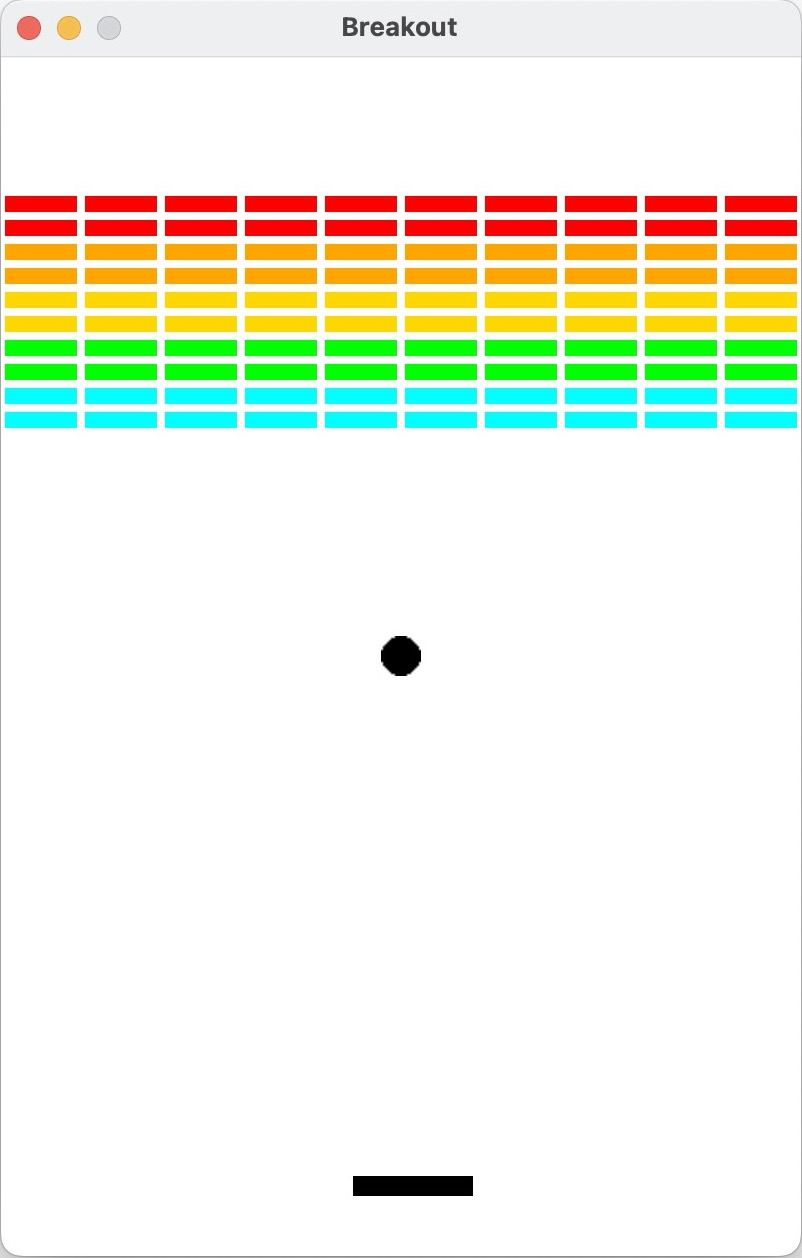
\includegraphics[width=.5\textwidth, clip]{images/ch10/breakout.jpg}};
  \drawshadow{image}
\end{tikzpicture}
\caption{} 
\label{fig:breakout}
\end{figure}
%

\fEn{Arcade} လိုက်ဘရီနဲ့ ရေးမှာပါ။ \fEn{Arcade} လိုက်ဘရီဟာ \fEn{inheritance} ကို အခြေခံထားတယ်။ \fCode{Window}\fEn{,} \fCode{View}\fEn{,} \fCode{Sprite} စတဲ့ ကလပ်စ်တွေကို လိုက်ဘရီကပေးထားတယ်။ ဂိမ်းတစ်ခုရေးတဲ့အခါ ဒီကလပ်စ်တွေကို \fEn{inherit} လုပ်ပြီး လိုအပ်တဲ့ မက်သဒ်တွေကို \fEn{override} လုပ်ပေးရုံပဲ။ လိုက်ဘရီက ပရိုဂရမ်ကို အကြမ်းထည် စထရက်ချာ ချထားပေးတယ်။ အဲ့ဒီ စထရက်ချာထဲမှာ ကိုယ်တိုင်စိတ်ကြိုက် ဖန်တီးချင်တဲ့နေရာတွေကို ပြင်ဆင်ဖြည့်စွက်လို့ရအောင် လုပ်ပေးထားတာလို့ ယူဆနိုင်တယ်။ ကြိုတင်သိထားဖို့ လိုအပ်တာတွေ တစ်ဆင့်ချင်း အရင်ကြည့်ရအောင်။

\subsection*{\fSubSecCodeBf{arcade.Window}}
\fCode{Window} ကလပ်စ်ဟာ ဂရပ်ဖစ် \fEn{window} တစ်ခုကို ကိုယ်စားပြုတယ်။ ဂရပ်ဖစ်ရုပ်ပုံတွေ ဆွဲဖို့နဲ့ အန်နီမေးရှင်း လုပ်ဖို့ လိုအပ်တာတွေ ဒီကလပ်စ်မှာ ထောက်ပံပေးထားတယ်။ ဒါ့အပြင် မောက်စ်၊ ကီးဘုဒ် စတဲ့ \fEn{input device} တွေနဲ့ ဂိမ်းကို ကွန်ထရိုးလ်လုပ်လို့ရစေမဲ့ နည်းလမ်းတွေလည်း ပါတယ်။

\fEn{Arcade} ပရိုဂရမ်တစ်ခုကို \fEn{run} တဲ့အခါ \fCode{Window} မှာ ပါတဲ့  \fCode{on\_draw} မက်သဒ်ကို တစ်စက္ကန့် အကြိမ် ခြောက်ဆယ် ခေါ်ပေးတယ်။ သူ့နဂိုအတိုင်း \fCode{on\_draw} မက်သဒ်က ဘာမှ လုပ်ဆောင်မပေးဘူး။ ကိုယ့်လိုချင်တဲ့ ဂရပ်ဖစ်ပုံ ဖော်ဖို့ \fCode{Window} ကို \fEn{inherit} လုပ်ပြီး \fEn{override} လုပ်ပေးရမယ်။  အပြာရောင် ဘောလုံးတစ်ခု အလယ်ဗဟိုမှာ ဆွဲမယ်ဆိုပါစို့ $\ldots$

%
\begin{py}
# File: arcade_blue_circle.py
import arcade
from arcade.color import *

WIN_WIDTH = 640
WIN_HEIGHT = 480

class MyGame(arcade.Window):

    def __init__(self, width, height, title):
        super().__init__(width, height, title)
        arcade.set_background_color(arcade.color.ALMOND)

    def on_draw(self):
        self.clear()
        arcade.draw_circle_filled(WIN_WIDTH / 2, WIN_HEIGHT / 2, 20, BLUE)

window = MyGame(WIN_WIDTH, WIN_HEIGHT, "Show Blue Circle")
arcade.run()
\end{py}
%
\fCode{on\_draw} ကို အခုလို  \fEn{override} လုပ်နိုင်ပါတယ်။ ဒီပရိုဂရမ် \fEn{run} တဲ့အခါ \fCode{on\_draw} ကို တစ်စက္ကန့်တိုင်း တစ်စက္ကန့်တိုင်းမှာ အကြိမ်ခြောက်ဆယ် \fEn{(60 frames per second)} တောက်လျှောက် ခေါ်နေမှာပါ။ ပရိုဂရမ် \fEn{window} မပိတ်မချင်းပေါ့။ ဒီလိုဖြစ်အောင် \fEn{Arcade} လိုက်ဘရီက လုပ်ပေးထားတာ။ ဒီအတွက် သီးခြားရေးဖို့ မလိုဘူး။ \fCode{Window} ကလပ်စ်ကို \fEn{inherit} လုပ်ပြီး \fCode{on\_draw} ကို \fEn{override} လုပ်ပေးရင် ရပြီ။ \fCode{clear} မက်သဒ်ကိုလည်း \fEn{superclass} \fCode{Window} ကနေ ဆက်ခံရထားတာ။ \fEn{Window} ပေါ်မှာ ရှိတဲ့ ဂရပ်ဖစ်အားလုံးကို ရှင်းပေးပြီး သတ်မှတ်ထားတဲ့ နောက်ခံရောင် ဖြည့်ပေးတဲ့ မက်သဒ်ပါ။  အန်နီမေးရှင်းအတွက် ဒီမက်သဒ်က အရေးကြီးတယ်ဆိုတာ တွေ့ရပါမယ်။ 

မောက်စ် (သို့) ကီးဘုဒ်နဲ့ ဘောလုံးကို ရွှေ့လို့ရအောင်လည်း လုပ်လို့ရတယ်။ ခက်ခဲတဲ့ ကိစ္စတွေကို \fCode{Window} က အဆင်သင့် လုပ်ထားပေးတာပါ။ ဒါဟာ အထူးအဆန်း ဖြစ်နေနိုင်ပါတယ်။ ဘယ်လိုများလုပ်ထားလဲ အကြမ်းဖျဉ်း သဘောတရား နားလည်ချင်တယ်ဆိုရင် အောက်ပါ ဥပမာကို လေ့လာကြည့်ပါ 
%
\begin{py}
class ConsolePrinter:
    def __init__(self, times):
        self._times = times
        
    def do_before(self):
        print("Checking if everything is ready.")
        
    def do_after(self):
        print("Doing cleaning up.")

    def do_my_task(self):
        self.do_before()
        for i in range(self._times):
            self.my_task()
        self.do_after()

    # do nothing    
    def my_task(self):
        pass


class MyConsolePrinter(ConsolePrinter):
    def __init__(self, times, text):
        super().__init__(times)
        self._text = text

    # to print as you want
    def my_task(self):
        print(self._text)


printer = MyConsolePrinter(15, 'Hello')
printer.do_my_task()
\end{py}
%
\fCode{ConsolePrinter}  မှာ \fCode{my\_task} ကလွဲလို့ ကျန်မက်သဒ်တွေအားလုံး အပြည့်အစုံရေးထားတာ တွေ့ရမှာပါ။ \fCode{do\_my\_task} က \fCode{my\_task} ကိုခေါ်ထားတယ်။ \fCode{MyConsolePrinter} က ထုတ်ပေးချင်တဲ့ စာသားအတွက် \fCode{my\_task} ကို \fEn{override} လုပ်ထားတာကို ဂရုပြုပါ။ ဒီသဘောတရားအတိုင်း \fEn{Arcade} လိုက်ဘရီက \fCode{Window}\fEn{,} \fCode{View}\fEn{,} \fCode{Sprite} စတဲ့ ကလပ်စ်တွေကလည်း ဒီသဘောတရားပဲ။ ဂိမ်းတစ်ခုအတွက် လိုအပ်ချက်တွေကို ပြင်ဆင်ပေးထားတယ်။ ပုံစံချပေးထားတယ်။ အသုံးပြုသူက ဒီကလပ်စ်တွေကို \fEn{inherit} လုပ်ပြီး သူ့ဂိမ်း လိုအပ်ချက်အတိုင်း ဖြစ်အောင် မက်သဒ်တွေကို \fEn{override} လုပ်ပြီး စိတ်ကြိုက်ဖန်တီးယူရတာ။


\subsection*{အန်နီမေးရှင်း}
စောစောက ပရိုဂရမ်မှာ စက်ဝိုင်းကို ညာဘက်ဘက်အပေါ်ကို ရွေ့သွားအောင် အန်နီမေးရှင်း လုပ်မယ်ဆိုပါစို့။ \fCode{on\_draw} လုပ်တဲ့ အခါတိုင်းမှာ လက်ရှိ $x$ နဲ့ $y$ တန်ဖိုးကို နည်းနည်းချင်း တိုးပေးနိုင်ပါတယ်။ နမူနာအနေနဲ့ $x$ ကို \fEn{2 pixels} နဲ့ $y$ ကို \fEn{1 pixel} တိုးပေးပါမယ်။
%
\begin{py}
# File: arcade_moving_circle.py
import arcade
from arcade.color import *

WIN_WIDTH = 640
WIN_HEIGHT = 480
RADIUS = 15


class MyGame(arcade.Window):

    def __init__(self, width, height, title):
        super().__init__(width, height, title)
        self._circle_x = WIN_WIDTH / 2
        self._circle_y = WIN_HEIGHT / 2
        arcade.set_background_color(arcade.color.ALMOND)

    def on_draw(self):
        self.clear()
        self._circle_x += 2     # move 2 pixels to the right
        self._circle_y += 1     # move 1 pixels upwards
        arcade.draw_circle_filled(self._circle_x,
                                  self._circle_y,
                                  RADIUS,
                                  BLUE)


window = MyGame(WIN_WIDTH, WIN_HEIGHT, "Moving Circle")
arcade.run()
\end{py}
%


\subsection*{\fSubSecCodeBf{Sprite}}
ဂိမ်းတစ်ခုမှာ ပါဝင်တဲ့ ဇာတ်ကောင်တွေ၊ အရာဝတ္ထုပစ္စည်းတွေကို \fCode{Sprite} ကလပ်စ်ကို  \fEn{inherit} လုပ်ပြီး ကိုယ်စားပြုနိုင်ပါတယ်။ တစ်ခုနဲ့တစ်ခု ဝင်တိုက်တာ \fEn{(collision)} ၊  အပေါ်/အောက် (သို့) ဘယ်/ညာလှည့်တာ၊  အရာဝတ္ထုတွေကို အုပ်စုလိုက် ရွေ့လျားစေတာ စတာတွေကို အလွယ်တကူ လုပ်ဆောင်လို့ရအောင် \fCode{Sprite} ကလပ်စ်က ထောက်ပံ့ပေးထားတယ်။ \fEn{Window} ဘောင် တစ်ဖက်ဖက်နဲ့ ဝင်တိုက်ရင် ဘောလုံးက ပြန်ကန်ထွက်တဲ့ အန်နီမေးရှင်းဥပမာကို ကြည့်ရအောင် $\ldots$
%
\begin{py}
# File: arcade_bouncing_ball.py
import arcade
SCREEN_WIDTH = 680
SCREEN_HEIGHT = 480


class Ball(arcade.Sprite):

    def update(self):
        # rotate the sprite
        self.angle += 1
        # move the sprite
        self.center_x += self.change_x
        self.center_y += self.change_y

        if self.left < 0:
            self.change_x *= -1

        if self.right > SCREEN_WIDTH:
            self.change_x *= -1

        if self.bottom < 0:
            self.change_y *= -1

        if self.top > SCREEN_HEIGHT:
            self.change_y *= -1
\end{py}
%

\fCode{center\_x}\fEn{,} \fCode{center\_y} က \fCode{Sprite} ဗဟိုမှတ် တည်နေရာ။ \fCode{change\_x}\fEn{,} \fCode{change\_y} က အန်နီမေးရှင်းလုပ်ရင် နည်းနည်းချင်း ရွှေ့ပေးရမဲ့ $x$ နဲ့  $y$ ပမာဏ။ \fCode{Sprite} အမြန်နှုန်းနဲ့ ဦးတည်ရာကို ဒီနှစ်ခုရဲ့ တန်ဖိုးနဲ့ ထိန်းညှိပေးနိုင်တယ်။ \fCode{left}\fEn{,} \fCode{right}\fEn{,} \fCode{top}\fEn{,} \fCode{bottom} \fEn{attribute} တွေကတော့   \fCode{Sprite} ရဲ့ ဘယ်/ညာ $x$ တန်ဖိုးနဲ့  အထက်/အောက် $y$ တန်ဖိုးတွေကို ဖော်ပြတယ်။ ဒီ ဗေရီရေဘဲလ်တွေ အားလုံးကို \fEn{superclass} \fCode{Sprite} ကနေ ဆက်ခံရရှိထားတာ။ 

ဘယ် (သို့) ညာဘက် ဘောင်နဲ့ ထိရင် \fCode{change\_x} ကို အပေါင်းအနှုတ် ပြောင်းပြန် လုပ်ပေးရပါမယ်။ အထက် (သို့) အောက် ဘောင်နဲ့ ထိရင် \fCode{change\_y} ကို ပြောင်းပြန် လုပ်ပေးရပါမယ်။ ပုံ (\fRefNo{\ref{fig:ch10bouncing}}) မှာ ကြည့်ပါ။

\fCode{Ball} ကလပ်စ်မှာ \mintinline{text}|__init__| မက်သဒ် မပါဘူး။ (\fEn{Subclass} မှာ \mintinline{text}|__init__| မပါရင် အော့ဂျက်ဖန်တီးတဲ့အခါ ဆက်ခံရရှိထားတဲ့ \fEn{superclass} \mintinline{text}|__init__| ကိုပဲခေါ်ပါတယ်)။ 

\begin{figure}[tbh!]
\begin{tikzpicture}
\draw [very thick] (0,0)--(10,0)--(10,6)--(0,6)--cycle;

\node at (3.5,4) [below] {$(+,+)$};
\node at (6.5,4) [below] {$(+,-)$};
\draw[-{Latex[length=3mm]}] (3.5,4)--(5,6);
\draw[-{Latex[length=3mm]}] (5,6)--(6.5,4);

\node at (4.5,2) [above] {$(-,-)$};
\node at (1.5,2) [above] {$(-,+)$};
\draw[-{Latex[length=3mm]}] (4.5,2)--(3,0);
\draw[-{Latex[length=3mm]}] (3,0)--(1.5,2);

\node at (8,4.5) [left] {$(+,-)$};
\node at (8,1.5) [left] {$(-,-)$};
\draw[-{Latex[length=3mm]}] (8,4.5)--(10,3);
\draw[-{Latex[length=3mm]}] (10,3)--(8,1.5);
\end{tikzpicture}
\caption{ဘောင်နဲ့တိုက်တဲ့အခါ velocity လက္ခဏာ ပြောင်းလဲပုံ} 
\label{fig:ch10bouncing}
\end{figure}



\fCode{MyGame} ကလပ်စ်မှာ ဒီ ဘောလုံးကို ဘယ်လို အသုံးပြုထားလဲ ဆက်စပ်ကြည့်ပါ။ 
\begin{py}
# File: arcade_bouncing_ball.py
class MyGame(arcade.Window):

    def __init__(self, width, height, title):
        super().__init__(width, height, title)

        self._ball = Ball('ball.png', 0.2)

        self._ball.center_x = SCREEN_WIDTH / 2
        self._ball.center_y = SCREEN_HEIGHT / 2
        self._ball.change_x = 2
        self._ball.change_y = 1
        arcade.set_background_color(arcade.color.AIR_FORCE_BLUE)

    def on_draw(self):
        self.clear()
        self._ball.draw()

    def on_update(self, delta_time):
        self._ball.update()


window = MyGame(SCREEN_WIDTH, SCREEN_HEIGHT, "Bouncing Ball")
arcade.run()
\end{py}
%

\fCode{Sprite} အော့ဘ်ဂျက် ဖန်တီးတဲ့အခါ \fEn{image file} နံမည်နဲ့ \fEn{scale factor} ထည့်ပေးရပါတယ်။ ဘောလုံးကို \fEnSnd{ball.png} ဖိုင်၊ \fEn{scale factor} $0.2$ နဲ့ 
%
\begin{py}
self._ball = Ball('ball.png', 0.2)
\end{py}
%
ဖန်တီးတယ်။  \fEn{Image file} က ကုဒ်ဖိုင်နဲ့ ဖိုဒါတစ်ခုထဲမှာ ရှိရပါမယ်။ ဒါက အလွယ်နည်းကို ပြောတာပါ။ အခြားဖိုဒါမှာ ထားလို့ရပေမဲ့ နည်းနည်း ပိုရှုပ်လို့။

\fCode{Sprite} ရွေ့လျားတာနဲ့ \fEn{collision} ဖြစ်တဲ့ ကိစ္စတွေအတွက် အဓိက ဂိမ်းလော့ဂျစ်ကို  \fCode{on\_update} မက်သဒ်မှာ ရေးပေးရမယ်။ ဒါလည်းပဲ တကယ်က ဆက်ခံထားတဲ့ \fCode{on\_update} ကို  \fEn{override} လုပ်တာပါ။  ဒီမက်သဒ်ကိုလည်း တစ်စက္ကန့် အကြီမ်ခြောက်ဆယ် အလိုအလျောက် ခေါ်ပေးပါတယ်။ ဒါပေမဲ့ \fCode{on\_draw}  ရည်ရွယ်ချက်ချင်း မတူပါဘူး။ \fCode{on\_draw} က စခရင်ကိုပဲ \fEn{refresh} လုပ်ပေးတာ။ တစ်နည်းအားဖြင့် \fEn{window} ပေါ်မှာ ဂရပ်ဖစ်ပုံပဲ ဖော်ပေးတာ။ ဂိမ်းလော့ဂျစ်နဲ့ သက်ဆိုင်တာတွေ မလုပ်ဘူး။ \fCode{on\_update} ကျတော့ ပုံဆွဲတဲ့ကိစ္စကို မလုပ်ဘူး။ ဂိမ်းလော့ဂျစ်သီးသန့် လုပ်ဆောင်တယ်။ ဒီမက်သဒ်နှစ်ခု လုပ်ဆောင်ပေးတဲ့ တာဝန်ကို ခွဲခြားထားရပါမယ်။ ဂိမ်းမှာပါဝင်တဲ့ \fCode{Sprite} အားလုံးရဲ့ \fEn{state} ကို \fEn{update} လုပ်ပေးခြင်းဟာ \fCode{on\_update} ရဲ့ အဓိကတာဝန်တွေထဲက တစ်ခုအပါအဝင် ဖြစ်တယ်။ အခုဥပမာမှာ ဘောလုံးရဲ့ \fEn{state} ကို
%
\begin{py}
self._ball.update()
\end{py}
%
ခေါ်ပြီး \fEn{update} လုပ်ပေးထားတယ်။

\fCode{on\_update} မက်သဒ် \fCode{delta\_time} ပါရာမီတာကို ရှင်းပြဖို့ ကျန်ပါသေးတယ်။ \fCode{on\_update} ကို ခေါ်တဲ့အခါ နောက်ဆုံးခါ်ခဲ့တဲ့ အချိန်နဲ့ အခုခေါ်တဲ့ အချိန်ကြား ကွဟချက်ကို \fCode{delta\_time} အနေနဲ့ ထည့်ပေးတယ်။ \fEn{Arcade} လိုက်ဘရီ နောက်ကွယ်က အလုပ်လုပ်ပုံ သဘောတရားအရ ထည့်ထားတဲ့ ပါရာမီတာဖြစ်ပြီး လိုက်ဘရီ သုံးတဲ့သူအနေနဲ့ အသေးစိတ်သိဖို့ မလိုအပ်ပါဘူး။ \fCode{on\_update} ကို \fEn{override} လုပ်တဲ့အခါ \fCode{delta\_time} ပါရာမီတာ မကျန်ခဲ့ရင် ရပါပြီ။


\subsection*{Event Handling}
မောက်စ်၊ ကီးဘုဒ်၊ \fEn{joystick} စတဲ့ \fEn{input device} တွေနဲ့ ဂိမ်းကို ထိန်းချုပ်ဖို့အတွက်လည်း \fCode{Window} ကလပ်စ်က လွယ်အောင်လုပ်ထားတယ်။ \fCode{on\_mouse\_motion}\fEn{,} \fCode{on\_mouse\_press}\fEn{,} \fCode{on\_key\_press} စတဲ့ မက်သဒ်တွေကို \fEn{override} လုပ်ရုံပါပဲ။ အဖြစ်အပျက် တစ်စုံတစ်ခု \fEn{(event)} ကို ပရိုဂရမ်က တုံ့ပြန်လုပ်ဆောင်‌ပေးတာကို \fEnEmp{event handling} လို့ ခေါ်တယ်။ ကီးဘုဒ် ကီးနှိပ်/လွှတ် လိုက်တာ၊ မောက်စ်ကလစ်နှိပ်/လွှတ် လိုက်တာ၊ မောက်စ်ရွှေ့တာ စတာတွေဟာ \fEn{event} ဥပမာတချို့ ဖြစ်တယ်။ ဒါတွေကို ပရိုဂရမ်က တုံ့ပြန်လုပ်ဆောင်ချင်တဲ့အခါ \fEn{event handling} ကို သုံးရပါတယ်။

ဒါက ဘောလုံးကို မောက်စ်နဲ့ ရွှေ့တဲ့ နမူနာပါ။ မောက်စ်ကို နှိပ်ထားပြီး ရွှေ့ရတာ \fEn{(dragging)} မဟုတ်ဘူး။ ဒီတိုင်း ပွိုင်တာရွေ့တဲ့ နောက်ကို ဘောလုံးက လိုက်နေမှာပါ။
%
\begin{py}
# File: arcade_m_move.py
class MyGame(arcade.Window):

    def __init__(self, width, height, title):
        super().__init__(width, height, title)
        self._ball = arcade.Sprite('ball.png', 0.2)
        self._ball.center_x = SCREEN_WIDTH / 2
        self._ball.center_y = SCREEN_HEIGHT / 2
        arcade.set_background_color(arcade.color.AIR_FORCE_BLUE)

    def on_draw(self):
        self.clear()
        self._ball.draw()

    def on_mouse_motion(self, x: int, y: int, dx: int, dy: int):
        self._ball.center_x = x
        self._ball.center_y = y
\end{py}
%
မောက်စ်ကို ရွှေ့ရင် မောက်စ်ပွိုင်တာရွေ့နေသ၍ \fCode{on\_mouse\_motion} ကို တစ်ခါပြီးတစ်ခါ အဆက်မပြတ် ခေါ်နေမှာပါ။ မောက်စ် ရပ်လိုက်ရင် ဒီမက်သဒ်ခေါ်တာလည်း ရပ်သွားမယ်။ ဒီလိုဖြစ်အောင် \fCode{Window} က လုပ်ပေးထားတာ။ \fCode{x} နဲ့ \fCode{y} က လက်ရှိ မောက်စ်ပွိုင်တာရဲ့ တည်နေရာ။ \fCode{dx} က ဒီမက်သဒ်ကို နောက်ဆုံးခေါ်ခဲ့တဲ့ အချိန်နဲ့ အခုခေါ်တဲ့ အချိန်အတွင်း ပြောင်းလဲသွားတဲ့ \fCode{x} ကွာဟချက်။ \fCode{dy} က ဒီမက်သဒ်ကို နောက်ဆုံးခေါ်ခဲ့တဲ့ အချိန်နဲ့ အခုခေါ်တဲ့ အချိန်အတွင်း ပြောင်းလဲသွားတဲ့ \fCode{y} ကွာဟချက်။ နောက်ဆုံးခေါ်ခဲ့တုံးက မောက်စ်က $(x_1, y_1)$ မှာ ရှိခဲ့တယ်၊ အခုခေါ်တဲ့အချိန် $(x_2, y_2)$ မှာ ဆိုပါစို့။  $dx= x_2 - x_1$\fEn{,} $dy= y_2 - y_1$ ဖြစ်တယ်။

မောက်စ် ကလစ်နှိပ်တဲ့အခါ တစ်ခုခု လုပ်မယ်ဆိုရင် \fCode{on\_mouse\_press} ကို \fEn{override} လုပ်ရပါမယ်။ ဒီမက်သဒ်ကိုတော့ ကလစ်နှိပ်တော့မှပဲ ခေါ်မှာပါ။  မောက်စ် ဘယ်ဘက် ကလစ်နှိပ်လိုက်တဲ့နေရာကို ဘောလုံး (ချက်ချင်း)ရောက်စေချင်ရင် အခုလို $\ldots$
%
\begin{py}
# File: arcade_m_press.py
def on_mouse_press(self, x, y, button, modifiers):
    if button == arcade.MOUSE_BUTTON_LEFT:
        self._ball.center_x = x
        self._ball.center_y = y
\end{py}
%

ကီးဘုဒ်နဲ့ ထိန်းချင်ရင် \fCode{on\_key\_press} ကို \fEn{override} လုပ်ရပါမယ်။ \fEnSnd{arcade\_k\_press.py} မှာ လေ့လာကြည့်ပါ။ မောက်စ် နှိပ်ထားပြီး ဘောလုံးကိုရွှေ့ \fEn{(dragging)} တာကို \fEnSnd{arcade\_m\_drag.py} ဖိုင်မှာ ကြည့်နိုင်ပါတယ်။

%Arcade’s Window class has a lot of built-in methods that are automatically called when needed. Methods for drawing, for responding to the keyboard, the mouse, and more. You can see all the methods by looking at the Window Class Documentation. But by default, these methods don’t do anything. We need to change that.

\subsection*{\fSubSecCodeBf{arcade.View}}
\fCode{arcade.View} ဟာ \fCode{Window} နဲ့ သဘောတရား အတော်လေးဆင်တူပါတယ်။ \fCode{Window} လိုပဲ စခရင်မှာ ဂရပ်ဖစ်ပုံဖော်ဖို့ \fCode{View} ကို သုံးလို့ရတယ်။ \fEn{Event handling} အတွက် \fEn{override} လုပ်ရတာတွေကလည်း \fCode{Window} နဲ့ တူတူပါပဲ။ ဒါပေမဲ့ \fCode{View} က သူ့ချည်း မရပ်တည်နိုင်ပါဘူး။ \fCode{View} ကို ပြပေးဖို့အတွက် \fEn{Window} တစ်ခုလိုပါတယ်။ \fCode{Window} တစ်ခုတည်းဟာ \fCode{View} အမျိုးမျိုးကို အလှည့်ကျ လဲပြီးပြလို့ရတယ်။ ဂိမ်းတစ်ခုမှာ \fEn{welcome screen, game over screen, pause screen} စသည်ဖြင့် ပြပေးဖို့လိုပါတယ်။ ဒီလို လိုအပ်ချက်မျိုးအတွက်ဆိုရင် \fEn{Arcade} မှာ \fCode{View} ကို အသုံးပြုရမှာပါ။  နမူနာကြည့်ရင် ပိုရှင်းသွားပါလိမ့်မယ်။

အောက်ပါဥပမာက ပထမ စစချင်း \fEn{Click to Start!} လို့ ပြနေမှာပါ။  ကလစ်နှိပ်လိုက်ရင် ဘောလုံးက စရွေ့ပါမယ်။ ကလစ်ထပ်နှိပ်လိုက်ရင် ဘောလုံးရွေ့နေတာ ပျောက်သွားပြီး \fEn{The End} စာသားပြပါတယ်။ \fCode{MsgView} က စာသားပြပေးဖို့အတွက်။
\fCode{MainView} က ဘောလုံး အန်နီမေးရှင်းအတွက်။ နှစ်ခုလုံး \fCode{arcade.Window} အစား \fCode{arcade.View} ကို \fEn{inherit} လုပ်ထားတာ သတိပြုပါ။


%
\begin{py}
# File: arcade_view_switch.py
import arcade
from arcade.color import *

WIN_WIDTH = 400
WIN_HEIGHT = 600


class MainView(arcade.View):
    def __init__(self):
        super().__init__()
        self._circle_x = WIN_WIDTH // 2   # move 2 pixels to the right
        self._circle_y = WIN_HEIGHT // 2  # move 1 pixels upwards
        self._next_view = None

    def on_draw(self):
        self.clear()
        self._circle_x += 1.3  # move 2 pixels to the right
        self._circle_y += 2    # move 1 pixels upwards
        arcade.draw_circle_filled(self._circle_x,
                                  self._circle_y,
                                  20,
                                  BLUE)

    def on_mouse_press(self, _x, _y, _button, _modifiers):
        """ If the user presses the mouse button, start the game. """
        self.window.show_view(self._next_view)


class MsgView(arcade.View):
    def __init__(self, msg):
        super().__init__()
        self._msg = msg
        self._next_view = None

    def on_draw(self):
        self.clear()
        arcade.draw_text(self._msg,
                         WIN_WIDTH / 2,
                         WIN_HEIGHT / 2,
                         RED,
                         font_size=20,
                         anchor_x="center")

    def on_mouse_press(self, _x, _y, _button, _modifiers):
        if self._next_view:
            self.window.show_view(self._next_view)


def main():
    window = arcade.Window(WIN_WIDTH, WIN_HEIGHT, "View Switch")
    end_view = MsgView("The End")
    start_view = MsgView("Click to Start!")
    main_view = MainView()

    start_view._next_view = main_view
    main_view._next_view = end_view
    window.show_view(start_view)
    arcade.run()


if __name__ == "__main__":
    main()

\end{py}
%

စောစောကပြောခဲ့သလို \fCode{View} ကို ပြဖို့ \fCode{Window} ရှိရပါမယ်။ \fEn{Arcade} ပရိုဂရမ်တစ်ခု \fEn{run} တဲ့အခါ \fCode{Window} တစ်ခုကတော့ ရှိကိုရှိရမှာပါ။ အဲဒီ \fCode{Window} ကို \fCode{View} က \fCode{self.window} နဲ့ ရည်ညွှန်းအသုံးပြုနိုင်တယ် (\fCode{View} ကို ဆက်ခံထားတဲ့  \fEn{subclass} မှာလည်း သုံးလို့ရတယ်)။ \fCode{Window} မှာ ပြချင်တဲ့ \fCode{View} ကို \fCode{window.set\_view} မက်သဒ်နဲ့ သတ်မှတ်ရတယ်။ \fCode{MsgView} နဲ့ \fCode{MainView} မှာ \fCode{on\_mouse\_press} ကို ဒီလို \fEn{override} လုပ်ထားတယ်

%
\begin{py}
def on_mouse_press(self, x, y, button, modifiers):
    if self._next_view:
        self.window.show_view(self._next_view)
\end{py}
%
ကလစ်နှိပ်ရင် \fCode{self.\_next\_view} ကို ပြောင်းပေးမှာပါ။ 

နောက်တစ်ခုက \fCode{View} အကျယ်နဲ့ အမြင့်ဟာ ၎င်းကိုပြပေးတဲ့ \fCode{Window} အပေါ် မူတည်တယ်။ ဒါကြောင့်   \fCode{View} တစ်ခုချင်းအတွက် အကျယ်၊ အမြင့် မသတ်မှတ်ဘူး။ \fCode{Window} အကျယ်နဲ့ အမြင့် သတ်မှတ်ရင် ရပြီ။

\fCode{main} မက်သဒ်မှာ \fCode{Window} တစ်ခု နဲ့ \fCode{View} သုံးခု ဖန်တီးထားတယ်။ \fCode{View} တစ်ခုကနေ တစ်ခု ပြောင်းလဲဖို့ အခုလို ချိတ်ဆက်ပေးထားတာ
%
\begin{py}
start_view._next_view = main_view
main_view._next_view = end_view
\end{py}
%
တွေ့ရမှာပါ။ \fCode{start\_view} ပေါ်မှာ ကလစ်နှိပ်ရင် \fCode{main\_view}\fEn{,} \fCode{main\_view} ပေါ်မှာ နှိပ်ရင် \fCode{end\_view} ကို ပြပေးမှာပါ (\fCode{on\_key\_press} မက်သဒ်နဲ့ ဆက်စပ်ကြည့်ပြီး နားလည်အောင်လုပ်ပါ)။

\section{Breakout တည်ဆောက်ခြင်း}
ဂိမ်း မတည်ဆောက်ခင် ကြိုတင်နားလည်ထားရမဲ့ \fEn{Arcade} သဘောတရား အတော်များများ ရှင်းပြခဲ့ပြီးပြီ။ တကယ် လက်တွေ့ ဂိမ်းရေးဖို့ပဲ ကျန်ပါတော့တယ်။  ပရိုဂရမ် အပြည့်အစုံကို စာမျက်နှာ (\fRefNo{\pageref{lst:breakoutfull}}) မှာ ကြည့်ပါ။ အခု တစ်ပိုင်းချင်း ခွဲထုတ် ရှင်းပြပါမယ်။ ဂိမ်းအတွက် လိုအပ်တဲ့ \fEn{constant} တွေကို ပထမဆုံး သတ်မှတ်ထားတယ်။ အများစုက တည်နေရာ၊ အရွယ်အစားနဲ့ သက်ဆိုင်တာတွေ။


%
\begin{py}
WIN_WIDTH = 400
WIN_HEIGHT = 600

# paddle size
PDL_WIDTH = 60
PDL_HEIGHT = 10
PDL_Y_OFFSET = 30    # distance between paddle and lower edge of window

BALL_RADIUS = 10
BRICKS_PER_ROW = 10
BRICK_ROWS = 10      # number of brick rows
BRICK_GAP = 4        # gap between bricks

# calculate and define constants for brick width and height
BRICK_WIDTH = ((WIN_WIDTH - (BRICKS_PER_ROW - 1) * BRICK_GAP)
               // BRICKS_PER_ROW)
LEFT_MARGIN = (WIN_WIDTH - (BRICK_WIDTH * BRICKS_PER_ROW +
                            BRICK_GAP * (BRICKS_PER_ROW - 1))) // 2
BRICK_HEIGHT = 8

# ß\fEn{Window} \fMM{အောက်ဘက် ဘောင်နဲ့ နံရံအောက်ခြေ အကွာအဝေး} ß
BRICK_Y_OFFSET = 414
# ß\fEn{Window} \fMM{ဗဟိုမှတ်} ß
CENTER_X = WIN_WIDTH // 2
CENTEr_Y = WIN_HEIGHT // 2
\end{py}
%


\subsection*{အုတ်ခဲစီခြင်း}
\fCode{setup\_bricks} က အုတ်ခဲတွေ နေရာတကျ စီပေးတဲ့ ဖန်ရှင်။ အုတ်ခဲကို \fCode{SpriteSolidColor} နဲ့ ဆွဲလို့ရတယ်။ ဒီကလပ်စ်က အရောင်အပြည့် ထောင့်မှန်စတုဂံပုံ  \fCode{Sprite} ပါပဲ။  \fEn{image} ဖိုင် ရှိဖို့ မလိုဘူး။ စီထားတဲ့ အုတ်ခဲအားလုံးကို \fCode{SpriteList} နဲ့ သိမ်းထားပြီး \fEn{return} ပြန်ပေးထားတယ်။
%
%
\begin{py}
def setup_bricks():
    colors = [CYAN, CYAN, GREEN, GREEN, GOLD, GOLD,
              ORANGE, ORANGE, RED, RED]
    # ß\fMM{အုတ်ခဲအားလုံး ထည့်ထားဖို့}ß SpriteList
    brick_lst = arcade.SpriteList()
    y = BRICK_Y_OFFSET + BRICK_HEIGHT // 2
    # 10 ß$\times$ß 10 bricks wall
    for i in range(BRICKS_PER_ROW):
        x = LEFT_MARGIN + BRICK_WIDTH // 2
        for j in range(BRICK_ROWS):
            brick = arcade.SpriteSolidColor(BRICK_WIDTH,
                                            BRICK_HEIGHT,
                                            colors[i])
            brick.center_x = x
            brick.center_y = y
            # ß\fMM{အုတ်ခဲတစ်ခဲချင်း}ß SpriteList ß\fMM{ထဲထည့်}ß
            brick_lst.append(brick)
            x += (BRICK_WIDTH + BRICK_GAP)
        y += (BRICK_HEIGHT + BRICK_GAP)
    return brick_lst
\end{py}
%
%
\fCode{SpriteList} ထဲမှာ \fCode{Sprite} တွေ တစ်စုတစ်စည်းတည်း သိမ်းထားတာဟာ ဘောလုံးနဲ့ ဝင်တိုက်မိတဲ့ အုတ်ခဲတွေ (တစ်ခုထက်ပိုနိုင်တယ်) ကို စစ်ထုတ်ဖို့ လွယ်ကူစေတယ်ဆိုတာ ခဏနေ တွေ့ရမှာပါ။ $\big\llbracket$တည်နေရာ အတွက်အချက် အသေးစိတ်နားလည်ချင်ရင်  စာမျက်နှာ (\fRefNo{\pageref{subsec:ch07chkbrd}}) မှ ကျားကွက်ခုံ ဥပမာကို ကြည့်ပါ$\big\rrbracket$။

\subsection*{ဘောလုံးနှင့် တာထွက် velocity}
ဘောလုံးအတွက် \fCode{Ball} ကလပ်စ်ကို အခုလို သတ်မှတ်ပါမယ်။ ဘောင်တွေကို တိုက်တဲ့အခါ ပြန်ကန်ထွက်အောင် လုပ်တဲ့နည်းလမ်းက ရှေ့မှာတွေ့ခဲ့တဲ့ ဥပမာကလိုပါပဲ။ \mintinline{text}|self.left < 0| ဖြစ်ရင် ဘယ်ဘက်ဘောင်နဲ့ တိုက်တာ၊ \mintinline{text}|self.right < WIN_WIDTH| ဆိုရင် ညာဘက်နဲ့တိုက်တာ စသည်ဖြင့်ပေါ့။ အထက်/အောက် ဘောင်နဲ့တိုက်တာလည်း ဒီသဘောတရားပါပဲ။
%
\begin{py}
class Ball(arcade.SpriteCircle):
    def update(self):
        self.center_y += self.change_y
        self.center_x += self.change_x

        if self.left < 0:
            self.change_x *= -1

        if self.right > WIN_WIDTH:
            self.change_x *= -1

        # hitting bottom edge doesn't bounce 
        if self.bottom < 0:
            pass

        if self.top > WIN_HEIGHT:
            self.change_y *= -1
\end{py}
%
ဒီကလပ်စ်က \fCode{arcade.SpriteCircle} ကို \fEn{inherit} လုပ်ထားတယ်။ \fCode{SpriteCircle} က အရောင်ဖြည့် စက်ဝိုင်းပုံ  \fCode{Sprite} အတွက်။  \fEn{image} ဖိုင် မလိုဘူး။

\fCode{setup\_ball} ကတော့ ဘောလုံးရဲ့ ကနဦးတည်နေရာနဲ့ တာထွက် \fEn{velocity} ကို အဓိက တွက်ချက် သတ်မှတ်ပေးတာပါ။ ဖန်တီးထားတဲ့ ဘောလုံးကိုလည်း \fEn{return} ပြန်ပေးတယ်။
%
\begin{py}
def setup_ball():
    ball = Ball(BALL_RADIUS, arcade.color.BLACK)
    ball.center_x = WIN_WIDTH // 2
    ball.center_y = WIN_HEIGHT // 2
    ball.change_y = -6
    random.uniform(1.0, 3.0)
    ball.change_x = random.uniform(1.0, 3.0) \
        if random.uniform(0.0, 1.0) <= 0.5 \
        else random.uniform(-1.0, -3.0)
    return ball
\end{py}
%
အစမှာ ဘောလုံးအောက်ကို ကျလာတဲ့အခါ ဦးတည်ရာက အောက်တည့်တည့်ကိုပဲ အမြဲတစ်သမှတ်တည်း ဖြစ်နေရင် သိပ်မကောင်းဘူး။ ငြီးငွေ့စရာဖြစ်နေမယ်။ ဘယ်ဘက်ကို ဦးတည် ဆင်းလာမှာလဲ ခန့်မှန်းလို့မရရင် ပိုမိုက်တယ်။ စိတ်လှုပ်ရှားဖို့ ပိုကောင်းတယ်။ ဒီအတွက် \fCode{change\_x} ကို $1.0$ ကနေ $3.0$ အတွင်းနဲ့  $-1.0$ ကနေ $-3.0$ အတွင်း \fEn{random} ထုတ်ထားတယ်။ \fCode{random.uniform} ဖန်ရှင် သုံးပါတယ်။ \fCode{change\_x} အနှုတ်တန်ဖိုးဆိုရင် ဘယ်ဘက်၊ အပေါင်းဆိုရင် ညာဘက်ကို ဦးတည်တယ်။ ဘယ်ဘက်လား၊ ညာဘက်လားကိုလည်း ငါးဆယ် ငါးဆယ် ဖြစ်ချင်တယ်။ ဒါကြောင့် 
%
\begin{py}
random.uniform(0.0, 1.0) <= 0.5
\end{py}
%
ဖြစ်ရင် အပေါင်းတန်ဖိုး ဖြစ်အောင် \mintinline{text}|random.uniform(1.0, 3.0)| နဲ့ ထုတ်ပေးတယ်။ မဟုတ်ရင်တော့ အနှုတ်တန်ဖိုး ထွက်အောင်လုပ်ထားတယ်။ ဒါကြောင့် စစချင်းမှာ ဘောလုံးကျလာတဲ့ လားရာက ပုံ (\fRefNo{\ref{fig:balldir}}) မှာ ပြထားတဲ့ နယ်ပယ်အတွင်းမှာပဲ ရှိပါမယ်။

\begin{figure}[tbh!]
\begin{tikzpicture}
    \filldraw[opacity=0.2, color=gray] (0,4) -- (3,0) -- (1,0) -- cycle;
    \filldraw[opacity=0.2, color=gray] (0,4) -- (-3,0) -- (-1,0) -- cycle;
    \filldraw (0,4) circle (0.25);
    \draw[very thick] (-3.25,0) -- (3.25,0);
    \foreach \x in {-3,...,3}
    {
        \draw (\x,0.15) -- (\x,0);
        \node at (\x,0) [below] {$\x$};
    }

\end{tikzpicture}
\caption{ဘောလုံးကျလာနိုင်တဲ့နေရာ} 
\label{fig:balldir}
\end{figure}

\subsection*{\fSubSecCodeBf{Breakout} Class}
\fCode{Breakout} ကလပ်စ်ကို ဆက်ကြည့်ရအောင်။ ဂိမ်းရဲ့ အဓိက \fCode{View} ဖြစ်ပြီး အရှုံးအနိုင်ဆုံးဖြတ်တာ၊ ဘောလုံးနဲ့ အုတ်ခဲ၊ ဘောလုံးနဲ့ \fEn{paddle} တိုက်မိတာ စတာတွေကို ဒီကလပ်စ်မှာ ရေးထားတာပါ။ \fEn{paddle} ကို မောက်စ်နဲ့  ရွှေ့လို့ရအောင် \fCode{on\_mouse\_motion} ကလည်း ဒီထဲမှာပဲ။ $\big\llbracket$\fCode{Breakout} ကလပ်စ် အပြည့်အစုံကို စာမျက်နှာ (\fRefNo{\pageref{lst:breakout}}) မှာ ကြည့်ပါ$\big\rrbracket$။ 

\mintinline{text}|__init__| မက်သဒ်က သိပ်ရှုပ်ရှုပ်ထွေးထွေး မရှိဘူး။ မောက်စ်ပွိုင်တာ ပေါ်နေအောင်  \fCode{self.win\allowbreak dow.set\_mouse\_visible(True)} နဲ့ လုပ်ထားတယ်။ ဖျောက်ထားချင်ရင် \fCode{False} ထည့်ပေး။ \fEn{Instance variable} တွေ အားလုံးကို \fCode{None} ထည့်ထားတယ်။
%
\begin{py}
def __init__(self):
    super().__init__()

    arcade.set_background_color(WHITE)
    self.window.set_mouse_visible(True)
    self._ball = None
    self._paddle = None
    self._brick_lst = None
    self._brick_remains = None
    self._next_view = None
\end{py}
%

\fEn{Initialization} ကို \fCode{setup} မက်သဒ်မှာ အဓိက လုပ်ထားတယ်။ \mintinline{text}|__init__| မှာ ဘာလို့ မလုပ်လဲ မေးစရာရှိတယ်။ \mintinline{text}|__init__| မက်သဒ်က အော့ဘ်ဂျက် ဖန်တီးတဲ့အခါမှာပဲ အလိုအလျောက်ခေါ်ပေးတာ။ တိုက်ရိုက်ခေါ်ရတဲ့ မက်သဒ်မဟုတ်ဘူး။ ရှုံးသွားလို့ (သို့) နိုင်သွားလို့ နောက်တစ်ခါ ပြန်ဆော့ချင်ရင် အစအနေအထား ဖြစ်အောင် \fCode{setup} မက်သဒ်ကို ခေါ်လို့ရမယ်။ (ဒီတော့ \fCode{Breakout} အော့ဘ်ဂျက် အသစ်တစ်ခု ဖန်တီးတာ၊ \mintinline{text}|__init__| ကို တိုက်ရိုက်လည်း မခေါ်ဘဲ ပြန်စချင်ရင် \fCode{setup} ကို ခေါ်လို့ရမယ်)။ ရှေ့မှာတွေ့ခဲ့တဲ့ \fCode{setup\_ball}\fEn{,} \fCode{setup\_paddle}\fEn{,} \fCode{setup\_bricks} တို့ကို တစ်ဆင့် ပြန်ခေါ်ထားတာ တွေ့ရမယ်။ \fCode{\_brick\_remains} က လက်ကျန်အုတ်ခဲ အရေအတွက် မှတ်ထားဖို့။ အုတ်ခဲ တစ်လုံးပျက်သွားတိုင်း တစ်လျှော့ပေးရမယ်။

%
\begin{py}
def setup(self):
    self._paddle = arcade.SpriteSolidColor(PDL_WIDTH,
                                            PDL_HEIGHT,
                                            BLACK)
    self._paddle.bottom = PDL_Y_OFFSET
    self._paddle.center_x = CENTER_X

    self._ball = setup_ball()
    self._brick_lst = setup_bricks()
    self._brick_remains = 20
\end{py}
%

\fCode{draw} မက်သဒ်က ဂိမ်းမှာပါတဲ့ အုတ်နံရံ၊ ဘောလုံးနဲ့ \fEn{paddle} ပြားတို့ကို ဆွဲတယ်။ ဒီမက်သဒ်က \fCode{Breakout} ကလပ်စ်မှာ ထပ်ဖြည့်ထားတာ။ \fCode{View} ကလပ်စ်ရဲ့ တစ်စက္ကန့် အကြိမ်ခြောက်ဆယ် ခေါ်နေမဲ့  \fCode{on\_draw} ကို \fEn{override} လုပ်တာ မဟုတ်ဘူး။ \fCode{draw} ကို ခွဲထုတ်ထားရတာက လိုတဲ့အချိန်မှာ ကိုယ်တိုင်ခေါ်လို့ရအောင် ရည်ရွယ်တာပါ။ 
%
\begin{py}
def on_draw(self):
    self.draw()

def draw(self):
    self.clear()
    self._paddle.draw()
    self._brick_lst.draw()
    self._ball.draw()
\end{py}
%

ဂိမ်းရဲ့ အဓိကလော့ဂျစ်ကို \fCode{on\_update} မက်သဒ်မှာ တွေ့ရမှာပါ။ \fCode{View} ကလပ်စ်ရဲ့ \fCode{on\_update} ကို \fEn{override} လုပ်ပေးတာပါ။
%
\begin{py}
def on_update(self, delta_time):
    self._ball.update()
    self._paddle.update()
    self._brick_lst.update()
    bricks_hit = arcade.check_for_collision_with_list(self._ball,
                                                        self._brick_lst)
    if len(bricks_hit) > 0:
        self._ball.change_y *= -1
    for brick in bricks_hit:
        brick.remove_from_sprite_lists()
        self._brick_remains -= 1

    if self._brick_remains == 0:
        self._next_view._msg = "You Win!"
        self.window.show_view(self._next_view)

    if self._ball.center_y <= PDL_Y_OFFSET:
        self._next_view._msg = "You Lost!"
        self.window.show_view(self._next_view)

    if (arcade.check_for_collision(self._ball, self._paddle)
            and self._ball.change_y < 0):
        self._ball.change_y *= -1
\end{py}
%
\fCode{on\_update} ကို တစ်စက္ကန့် အကြိမ်ခြောက်ဆယ် အဆက်မပြတ် အလိုအလျောက် ခေါ်ပေးတယ်လို့ ပြောခဲ့တာ ပြန်အမှတ်ရမယ် ထင်ပါတယ်။ ဂိမ်းရဲ့ \fEn{state} ကို ဒီမက်သဒ် တစ်ကြိမ်ခေါ်တိုင်း \fEn{update} လုပ်ပေးရပါမယ်။ ဒါဟာ ဂိမ်းတစ်ခုရဲ့ အချိန်နဲ့အမျှ ပြောင်းလဲနေတဲ့ အရာအားလုံးအတွက် အဓိကသော့ချက်ပဲ။   ပထမဆုံး \fEn{Breakout} မှာပါတဲ့ ဘောလုံး၊ \fEn{paddle} နဲ့ အုတ်ခဲအားလုံးရဲ့ လက်ရှိအခြေအနေကို \fEn{update} လုပ်ရမယ်။ ဒီအတွက် ဂိမ်းမှာပါဝင်တဲ့ သက်ဆိုင်ရာ \fCode{Sprite} (သို့) \fCode{SpriteList} အားလုံးရဲ့ \fCode{update} မက်သဒ်ကို ခေါ်ပေးရမှာပါ။
%
\begin{py}
self._ball.update()
self._paddle.update()
self._brick_lst.update()
\end{py}
%

\fCode{check\_for\_collision\_with\_list} က ဝင်တိုက်မိတဲ့ \fCode{Sprite} တွေကို စစ်ထုတ်ပေးတဲ့ မက်သဒ်။ ဘောလုံးနဲ့ တိုက်မိတဲ့ အုတ်ခဲတွေကို လိုချင်တာ။ ဒီတော့ အခုလို ခေါ်ရမယ် 
%
\begin{py}
bricks_hit = arcade.check_for_collision_with_list(self._ball,
                                                  self._brick_lst)
\end{py}
%

အုတ်ခဲ (တွေ) နဲ့ ဝင်တိုက်ရင် ဘောလုံးကို အထက် (သို့) အောက် ပြန်ကန်ထွက်အောင် \fCode{change\_y} ကို လက္ခဏာ ဆန့်ကျင်ဘက် ပြောင်းပေးပါတယ်။
%
\begin{py}
if len(bricks_hit) > 0:
    self._ball.change_y *= -1
\end{py}
%
ဝင်တိုက်တဲ့ အုတ်ခဲတွေကို ဖျက်ပစ်ရပါမယ်။ ဖျက်လိုက်ရင် လက်ကျန်အုတ်ခဲလည်း လျော့သွားရမယ်။ ဒီအတွက် အခုလို
%
\begin{py}
for brick in bricks_hit:
    brick.remove_from_sprite_lists()
    self._brick_remains -= 1
\end{py}
%
တိုက်မိတဲ့ အုတ်ခဲတစ်ခဲချင်း ဖယ်ထုတ်ပါတယ်။

\subsection*{Start, Main and End \fSubSecCodeBf{View}s}
ပထမ စစချင်းမှာ ပုံ (\fRefNo{\ref{fig:breakout}}) မှာ တွေ့ရတဲ့ အနေအထားအတိုင်း ရှိနေမယ်။ ဒါပေမဲ့ စတာနဲ့ ဘောလုံးက ချက်ချင်းထွက်ရင် ဆော့ရတာ သိပ်အဆင်မပြေဘူး။ ကလစ်နှိပ်လိုက်မှ ဘောလုံးစထွက်မယ်ဆိုရင် ပိုကောင်းမယ်။ \fCode{StartView} ကို အခုလိုသတ်မှတ်ထားတယ်
%
\begin{py}
class StartView(arcade.View):
    def __init__(self):
        super().__init__()
        self._next_view = None

    def on_draw(self):
        self.clear()
        # ß Breakout \fMM{ရဲ့} setup \fMM{နဲ့} draw \fMM{ကိုခေါ်တာ}ß
        self._next_view.setup()
        self._next_view.draw()

    def on_mouse_press(self, x, y, button, modifiers):
        # ß\fMM{ကလစ်နှိပ်ရင်} Breakout View \fMM{ကို ပြောင်းပေးတာ}ß
        if self._next_view:
            self._next_view.setup()
            self.window.show_view(self._next_view)
\end{py}
%
စောစောကရှင်းပြခဲ့တဲ့ \fCode{Breakout} ဟာ ဂိမ်းရဲ့ အဓိက \fCode{View} ။ ဒါပေမဲ့ ဒီ \fCode{View} က စတာနဲ့ ဘောလုံးက ရွေ့မှာ \fCode{on\_draw} နဲ့  \fCode{on\_update} က ရပ်ထားလို့မရဘူး။ \fCode{View} ကို \fCode{Window} မှာ ပြပြီဆိုတာနဲ့ တောက်လျှောက် ခေါ်နေမှာ။ \fCode{StartView} က ရုပ်ပုံကို အငြိမ်ပဲ ပြပေးရမယ်။ ဖြစ်နိုင်တဲ့ နည်းလမ်းတစ်ခုက \fCode{Breakout} ရဲ့ \fCode{setup} နဲ့ \fCode{draw} ကို \fCode{StartView} ရဲ့ \fCode{on\_draw} ကနေ ခေါ်လို့ရပါတယ်။ \fCode{StartView} နဲ့ \fCode{Breakout} ကို \fCode{main} မက်သဒ်ထဲမှာ အခုလို ချိတ်ပေးထားပါမယ်။ 
%
\begin{py}
start_view = StartView()
game_view = Breakout()
# ...
start_view._next_view = game_view
window.show_view(start_view)
# ...
\end{py}
%

အရှုံးအနိုင် \fEn{You Win!/You Lose!} ပြဖို့ \fCode{EndView} ရဲ့ တာဝန်။ ရှုံး (သို့) နိုင်ရင် \fOpn{မက်ဆေ့ချ်} ပြပေးပြီး တစ်ခါထပ်ဆော့ချင်ရင် ကလစ်နှိပ်ရပါမယ်။  
%
\begin{py}
class EndView(arcade.View):
    def __init__(self):
        super().__init__()
        self._next_view = None
        self._msg = None

    def on_draw(self):
        self.clear()
        arcade.draw_text(self._msg,
                         WIN_WIDTH / 2,
                         WIN_HEIGHT / 2,
                         RED,
                         font_size=20,
                         anchor_x="center")

    def on_mouse_press(self, x, y, button, modifiers):
        if self._next_view:
            self.window.show_view(self._next_view)
\end{py}
%
\fCode{main} မက်သဒ်ထဲမှာ အခုလို ချိတ်ပေးထားပါတယ်
%
\begin{py}
end_view = EndView()
# ...
end_view._next_view = start_view
\end{py}
%


\subsection*{နိဂုံး}
ဒီအခန်းမှာ \fEn{Breakout} ဂိမ်းကို အသုံးချ ဥပမာအနေနဲ့ ထည့်ပေးထားတဲ့ ရည်ရွယ်ချက်က \fEn{Arcade} လိုက်ဘရီနဲ့ ဂိမ်းတွေ ဖန်တီးနိုင်ဖို့ အဓိက မဟုတ်ပါဘူး။ \fEn{Inheritance} ကို လိုက်ဘရီတွေမှာ အသုံးချလေ့ရှိတဲ့ ပုံစံတချို့ကို နားလည်သဘောပေါက်အောင်၊ သတိပြုမိအောင်၊ ဆက်စပ်မိအောင် အဓိက ရည်ရွယ်တာပါ။ စလေ့လာသူတွေအတွက် လွယ်လွယ်နဲ့ နားလည်နိုင်မယ်လို့တော့ မမျှော်လင့်နိုင်ဘူး။ စိတ်ရှည်ရှည်ထား အချိန်ပေးပြီး နားလည်သဘောပေါက်အောင် လေ့လာဖို့ လိုပါလိမ့်မယ်။ ပရိုဂရမ်အပြည့်အစုံကို အောက်မှာ ဖော်ပြပေးထားပါတယ်။ 

တည်နေရာ အတွက်အချက်တွေ နားမလည်လို့လည်း သင်္ချာကြောက်သူတွေ စိတ်ဓါတ်ကျစရာ မလိုပါဘူး။ အတွက်အချက်တွေ အကြမ်းဖျဉ်းလောက် နားလည်အောင် ကြည့်၊ ကျန်တဲ့ ပရိုဂရမ်းမင်းနဲ့ဆိုင်တဲ့ သဘောတရားတွေ အဓိကထား ကြည့်မယ်ဆိုရင်လည်း အတိုင်းအတာတစ်ခုထိ အကျိုးရှိမှာပါပဲ။

%
\begin{py}
ß\label{lst:breakoutfull}ß
import random
import arcade
from arcade.color import *

WIN_WIDTH = 400
WIN_HEIGHT = 600

PDL_WIDTH = 60
PDL_HEIGHT = 10
PDL_Y_OFFSET = 30    # distance between paddle and lower edge of window

BALL_RADIUS = 10
BRICKS_PER_ROW = 10
BRICK_ROWS = 10      # number of brick rows
BRICK_GAP = 4        # gap between bricks
BRICK_WIDTH = ((WIN_WIDTH - (BRICKS_PER_ROW - 1) * BRICK_GAP)
               // BRICKS_PER_ROW)
LEFT_MARGIN = (WIN_WIDTH - (BRICK_WIDTH * BRICKS_PER_ROW +
                            BRICK_GAP * (BRICKS_PER_ROW - 1))) // 2
BRICK_HEIGHT = 8
BRICK_Y_OFFSET = 414
CENTER_X = WIN_WIDTH // 2
CENTEr_Y = WIN_HEIGHT // 2

ß\label{lst:breakout}ß
class Breakout(arcade.View):
    def __init__(self):
        super().__init__()

        arcade.set_background_color(WHITE)
        self.window.set_mouse_visible(True)
        self._ball = None
        self._paddle = None
        self._brick_lst = None
        self._brick_remains = None
        self._next_view = None

    def setup(self):
        self._paddle = arcade.SpriteSolidColor(PDL_WIDTH,
                                               PDL_HEIGHT,
                                               BLACK)
        self._paddle.bottom = PDL_Y_OFFSET
        self._paddle.center_x = CENTER_X

        self._ball = setup_ball()
        self._brick_lst = setup_bricks()
        self._brick_remains = 20

    def on_draw(self):
        self.draw()

    def draw(self):
        self.clear()
        self._paddle.draw()
        self._brick_lst.draw()
        self._ball.draw()

    def on_update(self, delta_time):
        self._ball.update()
        self._paddle.update()
        self._brick_lst.update()
        bricks_hit = arcade.check_for_collision_with_list(self._ball,
                                                          self._brick_lst)
        if len(bricks_hit) > 0:
            self._ball.change_y *= -1
        for brick in bricks_hit:
            brick.remove_from_sprite_lists()
            self._brick_remains -= 1

        if self._brick_remains == 0:
            self._next_view._msg = "You Win!"
            self.window.show_view(self._next_view)

        if self._ball.center_y <= PDL_Y_OFFSET:
            self._next_view._msg = "You Lost!"
            self.window.show_view(self._next_view)

        if (arcade.check_for_collision(self._ball, self._paddle)
                and self._ball.change_y < 0):
            self._ball.change_y *= -1

    def on_mouse_motion(self, x, y, dx, dy):
        self._paddle.center_x = x


def setup_bricks():
    colors = [CYAN, CYAN, GREEN, GREEN, GOLD, GOLD,
              ORANGE, ORANGE, RED, RED]
    brick_lst = arcade.SpriteList()
    x = LEFT_MARGIN + BRICK_WIDTH // 2
    y = BRICK_Y_OFFSET + BRICK_HEIGHT // 2
    # 10 x 10 bricks wall
    for i in range(BRICKS_PER_ROW):
        for j in range(BRICK_ROWS):
            brick = arcade.SpriteSolidColor(BRICK_WIDTH,
                                            BRICK_HEIGHT,
                                            colors[i])
            brick.center_x = x + (j * (BRICK_WIDTH + BRICK_GAP))
            brick.center_y = y + (i * (BRICK_HEIGHT + BRICK_GAP))
            brick_lst.append(brick)
    return brick_lst


class Ball(arcade.SpriteCircle):
    def update(self):
        self.center_y += self.change_y
        self.center_x += self.change_x

        if self.left < 0:
            self.change_x *= -1

        if self.right > WIN_WIDTH:
            self.change_x *= -1

        # hitting bottom edge doesn't bounce
        if self.bottom < 0:
            pass

        if self.top > WIN_HEIGHT:
            self.change_y *= -1


def setup_ball():
    ball = Ball(BALL_RADIUS, arcade.color.BLACK)
    ball.center_x = WIN_WIDTH // 2
    ball.center_y = WIN_HEIGHT // 2
    ball.change_y = -6
    random.uniform(1.0, 3.0)
    ball.change_x = random.uniform(1.0, 3.0) \
        if random.uniform(0.0, 1.0) <= 0.5 \
        else random.uniform(-1.0, -3.0)
    return ball


class StartView(arcade.View):
    def __init__(self):
        super().__init__()
        self._next_view = None

    def on_draw(self):
        self.clear()
        self._next_view.setup()
        self._next_view.draw()

    def on_mouse_press(self, x, y, button, modifiers):
        if self._next_view:
            self._next_view.setup()
            self.window.show_view(self._next_view)


class EndView(arcade.View):
    def __init__(self):
        super().__init__()
        self._next_view = None
        self._msg = None

    def on_draw(self):
        self.clear()
        arcade.draw_text(self._msg,
                         WIN_WIDTH / 2,
                         WIN_HEIGHT / 2,
                         RED,
                         font_size=20,
                         anchor_x="center")

    def on_mouse_press(self, x, y, button, modifiers):
        if self._next_view:
            self.window.show_view(self._next_view)


def main():
    window = arcade.Window(WIN_WIDTH, WIN_HEIGHT, "Breakout")
    start_view = StartView()
    game_view = Breakout()
    end_view = EndView()

    start_view._next_view = game_view
    game_view._next_view = end_view
    end_view._next_view = start_view

    window.show_view(start_view)
    arcade.run()


if __name__ == "__main__":
    main()

\end{py}
%

\chapter{Exceptions and Exception Handling}
% syntax error or compile time error, 
% programmer error or logic error
% runtime error of external condition
    % can recover
    % cannot recover

တကယ့်လက်တွေ့ အသုံးချ ပရိုဂရမ်တွေမှာ ရာနှုန်းပြည့် အမှားကင်းစင်ဖို့ဆိုတာ မဖြစ်နိုင်ပါဘူး။ ဒီလိုလုပ်ပေးနိုင်တဲ့ နည်းပညာလည်း ခုချိန်ထိ မရှိသေးဘူး။ ဒါကြောင့် ပရိုဂရမ်တွေဟာ \fEn{bug} အနည်းနဲ့အများတော့ ပါကြတာပါပဲ။ ပရိုဂရမ်မာ အမှားကြောင့် ဖြစ်တဲ့ \fEn{bug} တွေ လုံးဝမရှိအောင် တစ်နည်းတစ်လမ်းနဲ့ လုပ်နိုင်တယ် ဆိုအုံးတော့၊ တစ်ဖက်မှာ ပရိုဂရမ်တစ်ခုကို အသုံးပြုနေစဉ်  ကြုံတွေ့ရတဲ့ ချွင်းချက် အခြေအနေတွေက ရှိနေပါသေးတယ်။ အီးမေးလ်ပို့တဲ့အချိန် နက်ဝပ်က ဒေါင်းနေတာ၊ ဖွင့်တဲ့ ဖိုင်က ပျက်နေတာ၊ သုညနဲ့ စားတာ \fEn{(division by zero)}၊ မမ်မိုရီမလုံလောက်တာ စတဲ့ကိစ္စတွေ ပရိုဂရမ် အလုပ်လုပ်နေစဉ် ကြုံတွေ့ရတတ်ပါတယ်။ ဒီလို ပြဿနာတွေက အမြဲတမ်း ဖြစ်နေတာတော့ မဟုတ်ဘူး၊ ရံဖန်ရံခါပဲ ဖြစ်တာဆိုပေမဲ့ ရှောင်လွှဲလို့ (သို့) လုံးဝမဖြစ်အောင် ကာကွယ်လို့လည်း မရပြန်ဘူး။ ဒီလို အဖြစ်အပျက်တစ်ခု ဖြစ်လာခဲ့ရင် ပရိုဂရမ်က လိုအပ်သလို စီမံထိန်းကွပ်လို့ရအောင် ရိုးရှင်းတဲ့ နည်းစနစ်တစ်မျိုး ရှိသင့်ပါတယ်။ ပရိုဂရမ်ရဲ့ ပုံမှန်စီးဆင်းမှု (ပြဿနာ မဖြစ်ခဲ့ရင် ပုံမှန်အတိုင်း လုပ်ဆောင်သွားမဲ့ ကုဒ်တွေကို ဆိုလိုတာ) လမ်းကြောင်းကိုလည်း ဒီနည်းစနစ်ကြောင့် အများကြီးပိုပြီး မရှုပ်ထွေးစေသင့်ဘူး။ တစ်နည်းအားဖြင့် ပြဿနာ မဖြစ်ရင် လုပ်ဆောင်မဲ့ အပိုင်းနဲ့ ဖြစ်ခဲ့ရင် လုပ်ဆောင်ရမဲ့ အပိုင်း ရောထွေးမနေသင့်ဘူး။ ခွဲခြားထားရပါမယ်။

ဒီလို လိုအပ်ချက်တွေကို ဖြည့်ဆည်းပေးနိုင်တဲ့ နည်းလမ်းတွေထဲက အသုံးအများဆုံး တစ်ခုကတော့ \fEnEmp{exception-handling} \fEn{mechanism} ပါပဲ။ ခေတ်ပေါ် \fEn{programming language} အားလုံးလိုလိုမှာ  ထောက်ပံပေးထားပါတယ်။ တချို့ \fEn{language} တွေမှာ အခြားနည်းလမ်းတွေ အသုံးပြုတာ တွေ့ရပေမဲ့ လက်တွေ့မှာ အခုပြောတဲ့ \fEn{exception-handling} လောက် မတွင်ကျယ်သေးဘူး။ 

\fEnEmp{Exception-handling} သဘောတရားကို ဒီအခန်းမှာ အသေးစိတ် လေ့လာကြမှာပါ။ အောက်ပါအတိုင်း အပိုင်းတွေခွဲ လေ့လာကြမှာပါ။
%
\begin{itemize}
    \item \fEn{Raising exception}
    \item \fEn{Handling exception}
    \item \fEn{Control flow} 
    \item \fEn{Built-in exception class hierarchy}
    \item \fEn{User-defined exceptions}
    \item \fEn{Handling multiple exceptions}
\end{itemize}
%




\section{Raising Exception}
ဖန်ရှင်တစ်ခုဟာ ပြဿနာတစ်ခုခုကြောင့် သူ့တာဝန် ပြီးမြောက်အောင်မြင်အောင် ဆက်လက်လုပ်ဆောင်ဖို့ မဖြစ်နိုင်တဲ့အခါ \fEn{exception} တစ်ခုကို  \fEn{raise} လုပ်နိုင်ပါတယ်။ (မြန်မာလိုတော့ \fEn{exception} တက်အောင် လုပ်တာလို့ ပြောလေ့ရှိတယ်)။ အောက်ပါ \fCode{fun\_c} ဟာ အကြိမ်တစ်ရာမှာ (၅၀) လောက် \fCode{IOError} \fEn{exception} တက်အောင်  တမင်ရည်ရွယ် လုပ်ထားတယ်။ (ဥပမာပြဖို့ အတွက်ပါ။ လက်တွေ့မှာ ဒီလိုလုပ်ဖို့ အကြောင်းမရှိပါဘူး)။ \fEn{Random number} ထုတ်ပြီး \fEn{simulate} လုပ်ထားတယ်။ အင်တာနက်ကနေ ဒေတာတချို့ ဖတ်ပေးတဲ့ ဖန်ရှင်လို့ ယူဆချင် ယူဆပါ။  လိုင်း မကောင်းတဲ့ ဒေသမှာဆိုတော့ ဒီဖန်ရှင်က မကြာခဏ ပြဿနာပေးတယ်ပေါ့။  

%
\begin{py}
import random

def fun_c():
    print('Starting fun_c...')
    # simulate IOError, will fail 50% of the time
    if random.uniform(0.0, 1.0) <= 0.5:
        raise IOError("Failed to read!")
    print('fun_c ends!')
\end{py}
%
\fCode{fun\_c} ကို \fCode{main} ကနေ ခေါ်ပြီး အကြိမ်အနည်းငယ် \fEn{run} ကြည့်ပါ။
%
\begin{py}
def main():
    fun_c()
    print('main ends')

if __name__ == "__main__":
    main()
\end{py}
%

အဆင်ပြေတဲ့ အခါမှာ အခုလို
\begin{codetxt}
Starting main...
Starting fun_c...
fun_c ends!
main ends!
\end{codetxt}
ထွက်တယ်။ \fEn{Exception} တက်ရင်တော့ ဒီလိုမျိုး  \fEn{error} \fOpn{မက်ဆေ့ချ်}တွေ
\begin{codetxt}
Traceback (most recent call last):
  File ".../ch11/how_exceptions_works1.py", line 19, in <module>
    main()
  File ".../ch11/how_exceptions_works1.py", line 14, in main
    fun_c()
  File ".../ch11/how_exceptions_works1.py", line 8, in fun_c
    raise IOError("Failed to read!")
OSError: Failed to read!
Starting main...
Starting fun_c...
\end{codetxt}
ကျလာမှာပါ။ \fCode{main()} ကနေ \fCode{fun\_c()} ခေါ်ပြီး အဲဒီမှာ \fCode{IOError} ဖြစ်သွားတယ်လို့ ဖော်ပြထားတာ တွေ့ရတယ်။ \fCode{(most recent call last)} လို့လည်း တွေ့ရတယ်။ အောက်ဆုံးမှာ နောက်ဆုံးခေါ်ခဲ့တဲ့ ဖန်ရှင်လို့ ဆိုလိုတာ (နောက်ဆုံး ခေါ်ခဲ့တာ \fCode{fun\_c})။ ဖန်ရှင်တစ်ခုမှာ \fEn{exception} တက်တဲ့အခါ (သို့) ဖန်ရှင်တစ်ခုက \fEn{exception} ကို \fEn{raise} လိုက်တဲ့အခါ ၎င်းဖန်ရှင်ကို ခေါ်တဲ့ ဖန်ရှင်တွေအားလုံး ‘တောက်လျှောက် \fEn{fail} ဖြစ်မယ်’။ အခုဥပမာမှာ \fCode{main} ကနေ \fCode{fun\_c} ကို ခေါ်တယ်။ \fCode{fun\_c} မှာ \fEn{exception} ဖြစ်တော့ \fCode{main} လည်း ပြီးအောင်ဆက် အလုပ်မလုပ်ပေးနိုင်ဘူး။ \fEn{fail} ဖြစ်သွားတယ်။

စောစောက \fOpn{မက်ဆေ့ချ်}တွေကို သေချာဂရုစိုက်ကြည့်ပါ။ \fCode{fun\_c} မှာဆိုရင် \fEn{exception} ဖြစ်စေတဲ့နေရာ အောက်ပိုင်းက စတိတ်မန့်တွေ၊ \fCode{main} မှာဆိုရင် \fCode{fun\_c} ကို ခေါ်ထားတဲ့နေရာရဲ့ အောက်က စတိတ်မန့်တွေ အလုပ်မလုပ်သွားဘူး (\fCode{main} အတွက် \fCode{fun\_c} ခေါ်တဲ့လိုင်းက \fEn{exception} ဖြစ်စေတဲ့နေရာ)။  အခုကိစ္စမှာ ဖန်ရှင်နှစ်ခုလုံးရဲ့ \fEn{exception} ဖြစ်တဲ့နေရာ အောက်ပိုင်းမှာ \fCode{print} စတိတ်မန့် တစ်ကြောင်းစီပဲ ရှိပါတယ်။ အခြားစတိတ်မန့်တွေ ရှိခဲ့ရင်လည်း အလုပ်လုပ်မှာ မဟုတ်ဘူး။

အကယ်၍ \fCode{main} က \fCode{fun\_a} ကိုခေါ်၊ \fCode{fun\_a} က တစ်ဆင့် \fCode{fun\_b} ကိုခေါ်၊ \fCode{fun\_b} ကနေမှ \fCode{fun\_c} ကို နောက်ဆုံး ခေါ်ထားရင် \fCode{fun\_c} မှာ \fEn{exception} ဖြစ်တဲ့အခါ \fCode{fun\_b} က စပြီး \fEn{fail} ဖြစ်မယ်။ ပြီးရင် သူ့ကိုခေါ်တဲ့ \fCode{fun\_a} ဆက် \fEn{fail} မယ်။ နောက်ဆုံးမှာ \fCode{fun\_a} ကိုခေါ်ထားတဲ့ \fCode{main} ဖန်ရှင် \fEn{fail} ဖြစ်ပြီး ပရိုဂရမ်တစ်ခုလုံး ရပ်ဆိုင်းသွားမှာ ဖြစ်တယ်။ ရှေ့စာပိုဒ်မှာ ပြောခဲ့တဲ့ ‘တောက်လျှောက် \fEn{fail} ဖြစ်မယ်’ ဆိုတာ အဲဒီလိုဖြစ်စဉ်ကို ဆိုလိုတာ။

%
\begin{py}
# fun_c ß\fEn{exception} \fMM{ဖြစ်ရင် သူ့ကို ခေါ်ထားတဲ့ ဖန်ရှင်အားလုံး} \fEn{fail} \fMM{ဖြစ်ပါမယ်}ß  
def main():
    print('Starting main...')
    fun_a()
    print('main ends!')

def fun_a():
    print('Starting fun_a...')
    fun_b()
    print('fun_a ends!')

def fun_b():
    print('Starting fun_b...')
    fun_c()
    print('fun_b ends!')

if __name__ == "__main__":
    main()
\end{py}
%

\fEn{Exception raise} လုပ်တာဟာ ဖန်ရှင်တစ်ခုက ၎င်းလုပ်ဆောင်ရမဲ့ တာဝန်ကို ပြဿနာ တစ်ခုခုကြောင့် ပြီးမြောက် အောင်မြင်အောင် မလုပ်ဆောင်နိုင်တော့ဘူးဆိုတာ ဖန်ရှင်ခေါ်တဲ့သူကို အသိပေးတဲ့ နည်းလမ်းတစ်မျိုးလို့ ယူဆနိုင်ပါတယ်။ ဖန်ရှင်တစ်ခုကနေ အစပြု ဖြစ်ပေါ်တဲ့ \fEn{exception} ဟာ အဲဒီဖန်ရှင်ကို ခေါ်ထားတဲ့ ကွင်းဆက် \fEn{(call chain)} တစ်လျှောက် ပါဝင်တဲ့ဖန်ရှင် တစ်ခုပြီးတစ်ခု \fEn{exception} ဖြစ်စေပြီး နောက်ဆုံးမှာ ပရိုဂရမ်တစ်ခုလုံးကို ရပ်တန့်သွားစေမှာပါ။ \fEn{Exception} ဖြစ်ခဲ့ရင်  ပရိုဂရမ်တစ်ခုလုံးကို ပြန့်မသွားဘဲ၊ မသက်ရောက်စေဘဲ ထိန်းကွပ်ပေးလို့ရတဲ့ နည်းလမ်းရှိရပါမယ်။ အဲဒါကတော့ \fEn{exception} ကို \fEnEmp{handle} လုပ်ပေးခြင်းပါပဲ။ 



 

\section{Handling Exception}
စောစောက ဥပမာမှာ \fCode{fun\_c} ကိုခေါ်တဲ့အခါ ဖြစ်နိုင်တဲ့ \fEn{exception} ကို \fCode{fun\_b} က အခုလို \fEn{handle} လုပ်နိုင်ပါတယ်။ 

%
\begin{py}
def fun_b():
    print('Starting fun_b...')
    try:
        fun_c()
        print("fun_c was successful!")
    except IOError as e:
        print(e)
        print("Poor connection!")
    print('fun_b ends!')
\end{py}
%
\fEn{Python} မှာ \fCode{try...except} က \fEn{exception handling} အတွက်ပါ။ \fEn{Exception} ဖြစ်နိုင်တဲ့ ဖန်ရှင်ကို ခေါ်တဲ့အခါ \fCode{try} ဘလောက်ထဲမှာ ခေါ်ရပါမယ် (ဖြစ်ခဲ့ရင် \fEn{handle} လုပ်မယ်ဆိုတဲ့ ရည်ရွယ်ချက်ရှိရင်ပေါ့)။ \fCode{except} ဘလောက်က \fEn{exception} ဖြစ်ခဲ့ရင် \fEn{handle} လုပ်မဲ့ ကိစ္စအတွက်။

%
\begin{py}
except IOError as e:
\end{py}
%
\fCode{IOError} က \fEn{handle} လုပ်မဲ့ \fEn{exception} အမျိုးအစားကို သတ်မှတ်တာ။ ဆိုလိုတာက \fCode{IOError} သီးသန့်ကိုပဲ \fEn{handle} လုပ်မယ်။ \fCode{IOError} မဟုတ်တဲ့ အခြား \fEn{exception} တွေကို \fEn{handle} မလုပ်ဘူး။ (ဒါနဲ့ ပါတ်သက်ပြီး နောက်ပိုင်းမှာ ထပ်ရှင်းပြမှာပါ)။ \fCode{e} က ဖြစ်ပေါ်တဲ့ \fCode{IOError} \fEn{exception} အတွက် ဗေရီရေဘဲလ်ပါ။ \fEn{Exception} ဖြစ်ရင် \fCode{fun\_c} က \fCode{raise} လုပ်လိုက်တဲ့ \fCode{IOError} အော့ဘ်ဂျက်ကို ဒီဗေရီရေဘဲလ်မှာ ထည့်ပေးမှာ ဖြစ်တယ်။ (\fEn{Python} မှာ \fCode{IOError}\fEn{,} \fCode{ValueError}\fEn{,} \fCode{NameError} စတဲ့ ကလပ်စ်တွေ ပါရှိပြီး ဖြစ်ပေါ်တဲ့ \fEn{exception} အမျိုးအစားအလိုက် သက်ဆိုင်ရာ \fEn{exception} အော့ဘ်ဂျက်ကို \fCode{raise} လုပ်ရတာပါ)။

စောစောက ဥပမာမှာ \fCode{fun\_b} ကို အထက်ပါအတိုင်း  \fEn{exception handling} ထည့်ပြီး စမ်းသပ်ကြည့်တဲ့အခါ \fEn{exception} ဖြစ်တဲ့အခါ အခုလို
\begin{codetxt}
Starting main...
Starting fun_a...
Starting fun_b...
Starting fun_c...
Failed to read!
Poor connection!
fun_b ends!
fun_a ends!
main ends!
\end{codetxt}
တွေ့ရမှာပါ။ \fCode{fun\_b} မှာ \fEn{exception handling} လုပ်ထားတဲ့အတွက်  \fCode{fun\_c} က \fEn{exception} ဖြစ်ခဲ့ရင် အဲ့ဒီ \fEn{exception} ဟာ \fCode{fun\_a} နဲ့ \fCode{main} ဆီကို ထပ်ဆင့် မကူးစက်သွားတော့ဘူး။ \fEn{Exception handling} ဆိုတာ ပရိုဂရမ် အခြားအစိတ်အပိုင်းတွေကို \fEn{exception} မကူးစက်သွားအောင် ကွာရန်တင်းလုပ် ထိန်းချုပ်တာလို့ ယူဆနိုင်ပါတယ်။ 

\subsection*{Failure နဲ့ Exception ဘာကွာခြားလဲ}
အခုရှင်းပြပြီးခဲ့သလောက်မှာ \fEn{fail} ဖြစ်တာနဲ့ \fEn{exception} ဖြစ်တာ၊ ဒီသဘောတရားနှစ်ခု မရောထွေးသင့်ပါဘူး။ ဖန်ရှင်တစ်ခု \fEn{fail} ဖြစ်တယ်ဆိုတာ ပြဿနာတစ်ခုခုကြောင့် သူ့တာဝန်ကို အောင်မြင်အောင် မလုပ်နိုင်၊ အဲဒီ ပြဿနာကိုလည်း ကိုင်တွယ်ထိန်းကွပ်မထားတဲ့ အခြေအနေလို့ အကြမ်းဖျဉ်းယူဆပါ။ ဖန်ရှင်တစ်ခုက ပုံမှန်လမ်းကြောင်းအတိုင်း ပြီးမြောက်အောင် လုပ်ဆောင်သွားရင်၊ သို့မဟုတ် ပြဿနာ တစ်ခုခု ဖြစ်ခဲ့ရင်လည်း ဆက်မပြန့်သွားအောင် ကိုင်တွယ် ထိန်းကွပ်ပေးလိုက်ရင်  \fEn{successful} ဖြစ်တယ်လို့ ယူဆရပါမယ်။ \fEn{Exception} က \fEn{failure} ဖြစ်စေ ‘နိုင်’ တဲ့ အကြောင်းအရင်း။ ဒါပေမဲ့ \fEn{exception} ဖြစ်ရင် \fEn{fail} ဖြစ်မယ် ပုံသေမှတ်လို့မရဘူး။  \fEn{Exception} ကို \fEn{handle} လုပ်လိုက်ရင် \fEn{fail} မဖြစ်တော့ဘူး။

\fCode{fun\_c} \fEn{exception} ဖြစ်တော့ ခေါ်တဲ့ဖန်ရှင်အားလုံး တစ်ခုပြီးတစ်ခု ဆက်တိုက် \fEn{fail} ဖြစ်တယ်လို့ ရှေ့ပိုင်းမှာ ပြောခဲ့တယ်။ ဒါကို ပိုပြီးတိကျအောင် ပြောရမယ်ဆိုရင်  \fCode{fun\_c} \fEn{exception} ဖြစ်တဲ့အခါ သူ့ကိုခေါ်တဲ့ \fCode{fun\_b} ကိုလည်း \fEn{exception} ဖြစ်စေတယ်။ \fCode{fun\_b} က အဲဒီ \fEn{exception} ကို \fEn{handle} လုပ်ထားရင် \fEn{fail} မဖြစ်ဘူး။ မလုပ်ထားရင်တော့ သူကိုယ်တိုင်လည်း \fEn{fail} ဖြစ်ပြီး သူ့ကိုခေါ်တဲ့ \fCode{fun\_a} ကို \fEn{exception} ဆက်ဖြစ်စေပါတယ်။ \fCode{fun\_a} မှာလည်း ဒီသဘောအတိုင်း ဆက်ဖြစ်မှာပါ။ \fEn{Exception} \fEn{handle} လုပ်လိုက်ရင် \fEn{fail} မဖြစ်တော့ဘူး။ မလုပ်ထားရင်တော့ သူ့ကိုခေါ်တဲ့ \fEn{main} ဖန်ရှင်ကို \fEn{exception} ဆက်ဖြစ်စေပါလိမ့်မယ်။ 

% အကယ်၍ \fCode{fun\_b} က အဲ့ဒီ \fEn{exception} ကို \fEn{handle} လုပ်ထားရင် သူကိုယ်တိုင် \fEn{fail} မဖြစ်တော့ဘူး။ ၎င်းကိုခေါ်တဲ့ \fCode{fun\_a} 

နောက်ထပ် သိထားဖို့ အရေးကြီးတာ တစ်ခုက \fEn{exception} ဖြစ်တဲ့အခါ \fCode{try} ဘလောက်ထဲမှာပါတဲ့ အောက်က စတိတ်မန့်တွေကို ကျော်ပြီး \fCode{except} ဘလောက်ထဲ ချက်ချင်း ရောက်သွားမှာပါ။ \fCode{try} ဘလောက်ဟာ ပုံမှန် လုပ်ဆောင်မဲ့ လမ်းကြောင်း \fEn{(normal execution flow)} အတွက်ပါ။ \fEn{Exception} ဖြစ်ခဲ့ရင်တော့ ဒီလမ်းကြောင်းအတိုင်း ဆက်အလုပ်လုပ်လို့ မရတော့ဘူး။ ပုံမှန်မဟုတ်တဲ့ အခြေအနေမှာ လုပ်ဆောင်ရမဲ့ \fCode{except} ဘလောက်ကို လွှဲပြောင်း လုပ်ဆောင်ပေးရပါမယ်။ အခု ပြထားတာက ပုံမှန်အတိုင်း သွားမဲ့လမ်းကြောင်းပါ။
%
\begin{tikzpicture}[
  remember picture,
  overlay,
  annotation/.style={
    inner sep=0pt,
    outer sep=0pt,
    outer xsep=1mm,
    fill=yellow!80!black,
    text width=5cm
  },
  >={Stealth[inset=0pt, angle=30:7pt]}
]
\filldraw[lightgray!60,opacity=0.5] ([xshift=-1ex,yshift=1em] pic cs:ch11a1) rectangle ([xshift=.25ex,yshift=-.5em] pic cs:ch11a2);
\draw[->, thin] (pic cs:ch11a2)  ++(.25ex,.5ex) -- ++(0.5,0) |- ([yshift=0.5ex] pic cs:ch11a3);
\end{tikzpicture}
%
%
\begin{py}
def fun_b():
    print('Starting fun_b...')
    try:
        ß\tikzmark{ch11a1}ßfun_c()
        print("fun_c was successful!")ß\tikzmark{ch11a2}ß
    except IOError as e:
        print(e)
        print("Poor connection!")
    print('fun_b ends!')ß\tikzmark{ch11a3}ß
\end{py}
%
အောက်မှာပြထားတာက \fCode{IOError} ဖြစ်ခဲ့ရင် လုပ်ဆောင်မဲ့ပုံ (\fCode{fun\_c} ခေါ်ထားတဲ့လိုင်းကနေ \fCode{except} ကို ခုန်ပြီးရောက်သွားတာ သတိပြုပါ)။
%
\begin{tikzpicture}[
    remember picture,
    overlay,
    annotation/.style={
      inner sep=0pt,
      outer sep=0pt,
      outer xsep=1mm,
      fill=yellow!80!black,
      text width=5cm
    },
    >={Stealth[inset=0pt, angle=30:7pt]}
  ]
  
  \draw[->, thin] (pic cs:ch11b1)  ++(.25ex,.5ex) -- ++(12em,0) |- ([xshift=-.5ex,yshift=1ex] pic cs:ch11b3);
  \filldraw[lightgray!90,opacity=0.5] ([xshift=-1ex,yshift=1em] pic cs:ch11b2) rectangle ([xshift=.25ex,yshift=-.5em] pic cs:ch11b4);
  \draw[->, thin] (pic cs:ch11b4)  ++(.25ex,.5ex) -- ++(.5em,0) |- ([yshift=0.5ex]  pic cs:ch11b5);
  
\end{tikzpicture}
%
%
\begin{py}
def fun_b():
    print('Starting fun_b...')
    try:
        fun_c()ß\tikzmark{ch11b1}ß
        print("fun_c was successful!")
    except IOError as e:
        ß\tikzmark{ch11b2}ßprint(e)                  ß\tikzmark{ch11b3}ß
        print("Poor connection!")ß\tikzmark{ch11b4}ß
    print('fun_b ends!')ß\tikzmark{ch11b5}ß
\end{py}
%

ရှေ့က ဥပမာမှာ \fCode{fun\_b}  \fEn{handle} မလုပ်ဘဲ \fCode{fun\_a} က \fEn{handle} လုပ်လို့လဲရတယ်။ ဒါမှမဟုတ် \fCode{fun\_b} နဲ့ \fCode{fun\_a} မှာ \fEn{handle} မလုပ်ဘဲ \fCode{main} က လုပ်နိုင်ပါတယ်။ အောက်ပါအတိုင်း \fCode{fun\_a} မှာ \fEn{handle} လုပ်မယ်ဆိုပါစို့ 

%
\begin{py}
def fun_a():
    print('Starting fun_a...')
    try:
        fun_b()
        print("fun_b was successful!")
    except IOError as e:
        print(e)
        print("Poor connection!")
    print('fun_a ends!')


def fun_b():
    print('Starting fun_b...')
    fun_c()
    print('fun_b ends!')
\end{py}
%
\fCode{fun\_c} \fEn{exception} တက်ရင် \fEn{handle} မလုပ်ထားတဲ့ \fCode{fun\_b} လည်း  \fEn{exception} ဆက်ဖြစ်ပါမယ်။ အဲဒီ \fEn{exception} ကို \fCode{fun\_a} က \fEn{handle} လုပ်လိုက်တဲ့ အတွက် \fCode{main} ဆီကို ဆက်လက်မကူးစက် သွားတော့ပါဘူး။ \fEn{Output} အခုလို ထွက်တာ တွေ့ရမှာပါ။
%
\begin{codetxt}
Starting main...
Starting fun_a...
Starting fun_b...
Starting fun_c...
Failed to read!
Poor connection!
fun_a ends!
main ends!
\end{codetxt}
%
\fEn{Exception}  ဖြစ်တဲ့အခါ \fCode{"fun\_b ends!"} နဲ့ \fCode{"fun\_b was successful!"} အတွက် \fCode{print} စတိတ်မန့်တွေကို ကျော်သွားတာ သတိပြုကြည့်ပါ။



\section{ဘယ်နေရာမှာ handle လုပ်သင့်လဲ}
ဖန်ရှင်တွေ တစ်ခုပြီးတစ်ခုဆင့် ခေါ်ထားတဲ့အခါ \fEn{exception} ဖြစ်ခဲ့ရင် ဘယ်ဖန်ရှင်က \fEn{handle} လုပ်သင့်လဲ စဉ်းစားဆုံးဖြတ်ဖို့ လိုလာတယ်။ ဒီကိစ္စက ဘယ်မှာ \fEn{handle} လုပ်ရမယ် ပုံသေပြောလို့တော့ မရဘူး။ အခြေအနေနဲ့ လိုအပ်ချက်ပေါ် မူတည် ဆုံးဖြတ်ရတာမျိုး။ 
%
%
\begin{py}
def read_sensor():
    if random.uniform(0.0, 1.0) <= 0.2:
        raise IOError("Failed to read!")
    return random.randrange(1, 11)
\end{py}
%
ဒီဖန်ရှင်က \fEn{sensor device} တစ်ခုဆီကနေ ဒေတာဖတ်တာကို \fEn{simulate} လုပ်ထားတဲ့ ဖန်ရှင်ပါ။ \fEn{Sensor} ကြောင်လို့သော်လည်းကောင်း၊ \fEn{network} ကြောင့်သော်လည်းကောင်း (၂၀) ရာနှုန်း \fEn{fail} ဖြစ်တယ် ဆိုပါတော့။ 

\fEn{Sensor} တန်ဖိုး သုံးခုတစ်တွဲ ဖတ်ပြီး စောင့်ကြည့်လေ့လာရမယ်လို့ စိတ်ကူးကြည့်ပါ။ တန်ဖိုးသုံးခု အတွဲလိုက်ရအောင် ဖတ်ရမှာပါ။ \fEn{Exception} ဖြစ်လို့ သုံးခုမပြည့်သေးရင် ပြည့်တဲ့ထိ ထပ်ကြိုးစားရပါမယ်။  ဖတ်တဲ့အခါ တစ်ခါနဲ့တစ်ခါ စက္ကန့်တစ်ဝက်ခြား ဖတ်ပါတယ်။ တစ်ကယ့် လက်တွေ့မှာလည်း \fEn{sensor} ကနေ ဒေတာဖတ်တဲ့အခါ တရစပ် ဖတ်လေ့မရှိဘူး။ အချိန်အနည်းငယ် ခြားပြီးဖတ်တယ်။
%
\begin{py}
def read_3vals():
    vals = []
    while True:
        try:
            vals.append(read_sensor())
            if len(vals) == 3:
                return vals
        except IOError as err:
            pass
        time.sleep(0.5)
\end{py}
%
အခုကိစ္စအတွက် \fCode{read\_3vals} ဖန်ရှင်မှာ \fEn{handle} လုပ်ပေးရပါမယ်။ မလုပ်ဘဲထားရင် \fEn{fail} ဖြစ်ပြီး တန်ဖိုးသုံးခု ပြည့်အောင်ဖတ်လို့ မရနိုင်ဘူး။

အခုတစ်ခါ ကြားထဲမှာ ပြဿနာတစ်စုံတစ်ရာ မရှိဘဲ ဆက်တိုက် ဖတ်လို့ရတဲ့ တန်ဖိုးသုံးခု လိုချင်တယ် ယူဆပါ။ ဒီကိစ္စအတွက် \fEn{exception handle} မလုပ်ဘဲ ဖန်ရှင်တစ်ခု အခုလို ရေးနိုင်တယ်။ 

%
\begin{py}
def read_3_times():
    vals = []
    for i in range(3):
        vals.append(read_sensor())
        time.sleep(0.5)
    return vals
\end{py}
%
ဒီဖန်ရှင်က ပုံမှန်ဆိုရင်တော့  \fEn{sensor} ကို သုံးကြိမ်ဖတ်မှာပါ။ ဒါပေမဲ့ \fCode{read\_sensor} မှာ \fCode{IOError} \fEn{exception} ဖြစ်ခဲ့ရင် \fEn{handle} မလုပ်ထားတဲ့အတွက်  အခု \fCode{read\_3\_times} လည်း ဆက် \fEn{fail} ဖြစ်မယ်။ ကံကောင်းလို့ သုံးခါလုံး အဆင်ပြေခဲ့ရင်တော့ ဖတ်ထားတဲ့ တန်ဖိုးသုံးခုပါတဲ့ \fCode{vals} ကို ပြန်ပေးမှာပါ။  စောစောကဖန်ရှင်နဲ့ အဓိက ကွာခြားချက်ကို သတိပြုပါ။ \fCode{read\_3vals} က တန်ဖိုး သုံးခုပြည့်တဲ့ထိ ဖတ်ပေးရမှာပါ။ ဒါကြောင့် \fEn{exception handle} လုပ်ဖို့ လိုကို လိုတယ်။ ခုဖန်ရှင်က တန်ဖိုးသုံးခုကို ကြားထဲမှာ \fEn{fail} မဖြစ်ဘဲ ဆက်တိုက်  ဖတ်လို့ရမှပဲ ပြန်ပေးရမယ်။ ဒါကြောင့် \fEn{handle} မလုပ်ဘဲ ထားလို့ရတယ်။ \fCode{read\_3\_times} ကို ခေါ်တဲ့သူက \fEn{handle} လုပ်/မလုပ် ဆက်လက်ဆုံးဖြတ်နိုင်ပါတယ်။

ခုဏက ဖန်ရှင် အသုံးတည့်လာမဲ့ အခြေအနေတစ်ခု စဉ်းစားကြည့်ရအောင်။ သုံးခုတစ်တွဲ (၁၀) ခါဖတ်ရင် ဘယ်နှစ်ခါ \fEn{fail} ဖြစ်လဲ ဆန်းစစ်ကြည့်ချင်တယ် စိတ်ကူးကြည့်ပါ။ \fCode{read\_3\_times} ကို အခြေခံပြီး  \fCode{failure\_rate} ဖန်ရှင်ကို အခုလို သတ်မှတ်နိုင်ပါတယ်။ 
%
\begin{py}
def failure_rate():
    fail = 0
    for i in range(10):
        try:
            read_3_times()
        except IOError as e:
            fail += 1
    print(fail)
    return Fraction(fail, 10)
\end{py}
%
\fCode{read\_3\_times} က ဖြစ်ပေါ်တဲ့ \fEn{exception} ကို ဘယ်နှစ်ကြိမ် \fEn{fail} ဖြစ်လဲ ရေတွက်ဖို့ အသုံးချထားတာကို တွေ့ရပါတယ်။

%\fCode{read\_3\_times} ဟာ ဖြစ်ပေါ်နိုင်တဲ့ \fEn{exception} ကို \fEn{handle} မလုပ်တဲ့ ဖန်ရှင်တစ်ခုရဲ့ သာဓကဖြစ်တယ်။ သူ့အနေနဲ့ တန်ဖိုးသုံးခု ဆက်တိုက် ဖတ်လို့ရင် ပြန်ပေးတယ်။ အကယ်၍ မရခဲ့ရင်တော့  ၎င်းကိုယ်တိုင် \fEn{fail} ဖြစ်သွားမှာပါ။ ဒီတော့ ဖန်ရှင်ကောလ် ကွင်းဆက်တစ်လျှောက်မှာ ဘယ်နေရာမှာ \fEn{exception} ကို \fEn{handle} လုပ်မလဲ။ တစ်နေရာရာမှာ လုပ်တာတော့ လုပ်ရပါမယ်။ မလုပ်ရင် ပရိုဂရမ်တစ်ခုလုံး \fEn{fail} ဖြစ်သွားမှာ။

%\fCode{read\_3\_times} ကို ခေါ်တဲ့ ဖန်ရှင်က \fCode{read\_3\_times} \fEn{exception} ဖြစ်ရင် \fEn{handle} လုပ်နိုင်ပါတယ်။ ဒါမှမဟုတ် လိုအပ်ချက်အရ မလုပ်ဘဲ သူကိုယ်တိုင် \fEn{fail} အဖြစ်ခံတာလည်း ဖြစ်နိုင်တယ်။ \fEn{handle} မလုပ်ဘူး (\fEn{fail} ဆက်ဖြစ်မယ်) ဆိုရင်တော့ သူ့ကို ခေါ်ထားတဲ့ ဖန်ရှင်က \fEn{handle/fail} ဆက်လက် ဆုံးဖြတ်ရပါမယ်။ ဒီသဘောအတိုင်း တစ်ဆင့်ပြီးတစ်ဆင့် \fEn{handle} မလုပ်ဘဲ ဆက်သွားရင် နောက်ဆုံးမှာ \fEn{entry point} ဖြစ်တဲ့ \fCode{main} ဆီကို ရောက်သွားမှာပါ။ \fEn{main} ကလည်း \fEn{handle} မလုပ်ရင် \fCode{read\_sensor} က အစပြုခဲ့တဲ့ \fCode{IOError} \fEn{exception} ဟာ  ပရိုဂရမ်တစ်ခုလုံးကို ရပ်ဆိုင်းသွားစေမှာပါ။ (တကယ့်လက်တွေ့မှာတော့ ဒီလို အဖြစ်ခံလေ့ မရှိပါဘူး။ \fEn{Global exception handler} လို့ခေါ်တဲ့ ဘယ်ဖန်ရှင်ကမှ \fEn{handle} မလုပ်လို့ အပြင်ကို ပြန့်ထွက်လာတဲ့ \fEn{exception} တွေကို \fEn{handle} လုပ်တဲ့ အဆင့်တစ်ဆင့် ထည့်ထားလေ့ရှိတယ်)။



အခု လေ့လာတွေ့ရှိချက်တွေကို အနှစ်ချုပ်ပြန်ကြည့်ရင် ဖန်ရှင်တစ်ခု \fEn{exception} ဖြစ်တဲ့အခါ ၎င်းဖန်ရှင်ကို ခေါ်ထားတဲ့ ကွင်းဆက်တစ်လျှောက်လုံးက ဖန်ရှင်တွေ \fEn{fail} ဖြစ်နိုင်ပါတယ်။ \fEn{Fail} မဖြစ်အောင် ဖန်ရှင်တစ်ခုက \fEn{exception} ကို \fEn{handle} လုပ်ရပါမယ်။ ဘယ်ဖန်ရှင်က \fEn{handle} လုပ်ရမလဲကတော့ ပုံသေမရှိဘူး။ လိုအပ်ချက်ပေါ် မူတည်ပြီး ဆုံးဖြတ်ရလေ့ရှိတယ်။

% reading dates string from a file
    % all values must okay
    % fail if any not okay
    % all values okay and also log not okay values

% you are trying to get values from network every second
    % you want 

% m -> a -> b -> c and b try to return a special value if exception 
% m -> a -> b -> c and only the main handle exception and display appropriate message
% to the user 



\section{Exception Handling  နှင့် Control Flow}
\fEn{Exception handling} ကို ပရိုဂရမ်တစ်ခု ပုံမှန်စီးဆင်းရာ လမ်းကြောင်းနဲ့ ပုံမှန်အခြေအနေ မဟုတ်တဲ့အခါ စီးဆင်းရာလမ်းကြောင်း ခွဲခြားသတ်မှတ်ပေးတဲ့ နည်းစနစ်အဖြစ် ရှုမြင်နိုင်ပါတယ်။ \fEn{Exception} ဖြစ်တဲ့အခါ စီးဆင်းပုံကို အကြမ်းဖျဉ်းအားဖြင့် ပုံ (\fRefNo{\ref{fig:exphandling}}) မှာတွေ့ရသလို မြင်ကြည့်နိုင်ပါတယ်။

%
%
\begin{figure}[tbh!]
\begin{tikzpicture}[>={Stealth[inset=0pt, angle=30:7pt]}]
\foreach \i in {0,1,2,3}
{
  \pgfmathsetmacro\x{\i * (1.5 + 2)}
  \pgfmathsetmacro\y{7 - (\i * 1.25)}
  \def\myarr{{"a", "b", "c", "d"}}
  
  % How to draw rounded corners selectively
  %\filldraw[lightgray] {[rounded corners=5](\x,\y) -- ++(1.5,0)} -- ++(0,-1)  -- ++(-1.5,0){[rounded corners=5] --   cycle};
  %\begin{scope}[yshift=-1.5cm]
  %\filldraw[lightgray] (\x,\y) -- ++(1.5,0) {[rounded corners=5] -- ++(0,-1) -- ++(-1.5,0)} -- cycle;
  %\end{scope}
  
  \draw[thick, rounded corners=5, fill=lightgray!60] (\x,\y) rectangle ++(1.5,-2.5);
  % fun_a, fun_b, ..., etc
  \begin{scope}[xshift=0.75cm]
    \node at (\x,\y) [above] {$fun\_\pgfmathparse{\myarr[\i]}\pgfmathresult$};
  \end{scope}

  % fun_b(), fun_c(), etc and Bang! sign to indicate failure
  \def\myarrB{{"b", "c", "d"}}
  \begin{scope}[xshift=0.75cm,yshift=-1.25cm]
    \ifthenelse{\i < 3 }{\node at (\x,\y) {$fun\_\pgfmathparse{\myarrB[\i]}\pgfmathresult()$};
    }{}
    \ifthenelse{\i = 3 }{\node at (\x,\y) [starburst, draw=red, fill=yellow,
       starburst point height=0.4cm, font=\scriptsize, line width=1pt, inner sep=1.5pt] {\fEnBf{Bang!}};
    }{}
    \ifthenelse{\i = 2 }{\node at (\x,\y-0.8) [starburst, draw=red, fill=yellow,
       starburst point height=0.4cm, font=\scriptsize, line width=1pt, inner sep=1.5pt] {\fEnBf{Bang!}};
    }{}
  \end{scope}
  \ifthenelse{\i = 1 }{\draw[fill,color=gray] (\x+0.1,\y-1.5) rectangle (\x+1.4,\y-2.1);}{}  
  

  % draw arrows
  \ifthenelse{\i < 3 }{
    \draw[->,thin] [xshift=1.5cm,yshift=-1.25cm](\x,\y) to[out=45] ++(2,0);
  }{}
}
\draw[->,thin] (11,1.75) .. controls (9,1) and (6,1.5) .. (4.2,4);
\draw[->,thin] (3.4,3.5) .. controls (2.5,3.5) and (1.5, 4.5) .. (1.25,5.5);
\end{tikzpicture}
\caption{Exception Handling} 
\label{fig:exphandling}
\end{figure}
%
%

\fEnEmp{fun\_a}\fEn{,} \fEnEmp{fun\_b}\fEn{,} \fEnEmp{fun\_c}\fEn{,} \fEnEmp{fun\_d} တစ်ခုပြီးတစ်ခု ဆင့်ပြီး ခေါ်ထားတယ်။ မီးခိုးဖျော့ ထောင့်စွန်းဝိုင်း ထောင့်မှန်စတုဂံတွေက ဖန်ရှင်တစ်ခုစီကို ကိုယ်စားပြုတယ်။ အထဲမှာ ဖန်ရှင်ခေါ်ထားတာ တွေ့ရမယ်။ \fEn{Handle} လုပ်တာက \fEnEmp{fun\_b} မှာ (မီးခိုးရင့် ထောင့်မှန်စတုဂံအသေးလေးက \fEn{handle} လုပ်တဲ့ အပိုင်းလို့ ယူဆပါ)။

\fEnEmp{fun\_d} မှာ \fEn{exception} ဖြစ်တယ်။ \fEnEmp{fun\_c} လည်း \fEn{exception} ဆက်ဖြစ်ပြီး \fEn{fail} ဖြစ်မယ်။ သူ့ကို ခေါ်တဲ့ \fEnEmp{fun\_b} ကိုလည်း \fEn{exception} ဆက်ဖြစ်စေတယ်။ \fEnEmp{fun\_b} \fEn{handle} လုပ်လိုက်တဲ့ အတွက် \fEn{fail} မဖြစ်ဘူး။ \fEn{handle} လုပ်ပြီးသွားတော့  ၎င်းကို ခေါ်ခဲ့တဲ့ \fEnEmp{fun\_a} ထဲကို ပြန်ရောက်သွားပြီး \fEnEmp{fun\_a} ဆက်အလုပ်လုပ်မှာပါ။ 

ပုံအရ \fEn{exception} ဖြစ်တဲ့အခါ မူလစဖြစ်တဲ့နေရာကနေ \fEn{handle} လုပ်ထားတဲ့ အနီးဆုံး နေရာကို ခုန်ပြီးရောက်သွားတာကို တွေ့ရမှာပါ။ ဒီလို ခုန်သွားနိုင်တာဟာ \fEn{exception handling} မှာ အဓိကကျတဲ့ လုပ်ဆောင်ချက်ဖြစ်တယ်။ 

\subsection*{\fSecCodeBf{else} နှင့် \fSecCodeBf{finally}}
\fCode{try...except} အောက်မှာ \fCode{else} ဘလောက် နဲ့ \fCode{finally}  ဘလောက် ရှိနိုင်ပါတယ်။ \fEn{Exception} မဖြစ်တဲ့အခါမှပဲ လုပ်ဆောင်ချင်တဲ့ စတိတ်မန့်တွေကို \fCode{else} ဘလောက်ထဲမှာ ထည့်နိုင်ပါတယ်။ တစ်နည်း\allowbreak အားဖြင့် \fCode{try} ဘလောက် ပြဿနာမရှိဘဲ အောင်မြင်ပြီးစီးမှသာလျှင် \fCode{else} ဘလောက်ကို လုပ်ဆောင်မှာပါ။ \fEn{Exception} ဖြစ်ခဲ့ရင်တော့ လုပ်ဆောင်ပေးမှာ မဟုတ်ပါဘူး။
%
%
\begin{py}
def process_sensor_data():
    while True:
        try:
            val = read_sensor()
        except IOError as e:
            print(e)
        else:
            use_data(val)
            notify_if_necessary()
            print("Sensor data read successfully...")

        time.sleep(1)
        print("One iteration completed...")
\end{py}
%
% ---
%
\begin{codetxt}
Sensor data read successfully...
One iteration completed...
Sensor data read successfully...
One iteration completed...
Failed to read!
One iteration completed...
Failed to read!
\end{codetxt}
ဒီ \fEn{output} ကို လေ့လာကြည့်ရင် \fCode{else} ဘလောက်ကို \fEn{exception} မတက်မှပဲ လုပ်ဆောင်ပေးတယ်ဆိုတာ မြင်နိုင်မှာပါ။  \fCode{try...except...else} အပြင် အောက်ဆုံးက နှစ်ကြောင်းနဲ့ သဘောတရား မတူတာကိုလည်း သတိပြု ကြည့်ပါ။
%
%
\begin{py}
time.sleep(1)
print("One iteration completed...")
\end{py}
%
% 
\fEn{Exception} ဖြစ်ဖြစ်၊ မဖြစ်ဖြစ် ဒီ စတိတ်မန့် နှစ်ခုကိုက လုပ်ဆောင်ပေးတယ်။ \fCode{else} အပိုင်းကိုတော့ \fEn{exception} မတက်မှပဲ လုပ်ဆောင်တယ်။ 

စောစောက ဖန်ရှင်ကို \fCode{else} မပါဘဲ အောက်ပါကဲ့သို့ ရေးမယ်ဆိုရင်လည်း ရလဒ်အားဖြင့် တူတူပါပဲ။ \fCode{else} ကို အသုံးပြုရတဲ့ အဓိက အကြောင်းအရင်းက \fEn{exception} ဖြစ်စေနိုင်တဲ့ အပိုင်းနဲ့ မဖြစ်စေနိုင်တဲ့ အပိုင်း သီးသန့်ခွဲထားဖို့အတွက်ပါ။ 
%
%
\begin{py}
def process_sensor_data():
    while True:
        try:
            val = read_sensor()
            use_data(val)
            notify_if_necessary()
            print("Sensor data read successfully...")
        except IOError as e:
            print(e)
        time.sleep(1)
        print("processed single sensor data successfully...")
\end{py}
%
အခုပုံစံမှာက \fCode{try} ထဲက ဖန်ရှင်တွေထဲက ဘယ်ဟာက \fEn{exception} ဖြစ်စေတဲ့ အရင်းအမြစ်လဲ အလွယ်\allowbreak တကူ မသိနိုင်တော့ဘူး။ စောစောက \fCode{else} နဲ့ ပုံစံမှာက \fCode{read\_sensor} က \fEn{exception} ဖြစ်နိုင်တဲ့ ဖန်ရှင်ဖြစ်ရမယ်၊ အဲဒီ \fEn{exception} ကို \fEn{handle} လုပ်ထားတယ်ဆိုတာ သိသာ မြင်သာပါတယ်။%


%
\vspace{-1\baselineskip}
\begin{multicols}{2}%
\noindent
\begin{tikzpicture}[
  remember picture,
  overlay,
  annotation/.style={
    inner sep=0pt,
    outer sep=0pt,
    outer xsep=1mm,
    fill=yellow!80!black,
    text width=5cm
  },
  >={Stealth[inset=0pt, angle=30:7pt]}
]
\node at ([xshift=1.3cm]pic cs:ch11c0) [circle, aspect=2, draw=black, fill=green!50, font=\scriptsize, line width=1pt, inner sep=1.5pt] {\huge\ding{51}};
\draw[thin,rounded corners=5,fill=lightgray] ([yshift=1.5ex]pic cs:ch11c1) rectangle ([xshift=2cm]pic cs:ch11c2);
\draw[thin,rounded corners=5,fill=darkgray] ([yshift=1.5ex]pic cs:ch11c3) rectangle ([xshift=2cm]pic cs:ch11c4);
\draw[thin,rounded corners=5,fill=lightgray] ([yshift=1.5ex]pic cs:ch11c5) rectangle ([xshift=2cm]pic cs:ch11c6);
\draw[thin,rounded corners=5,fill=lightgray] ([yshift=1.5ex]pic cs:ch11c7) rectangle ([xshift=2cm]pic cs:ch11c8);
%\draw[->, thin] ([yshift=1.5cm,xshift=2.2cm]pic cs:ch11c2)  -- ([yshift=0.5ex,xshift=2.2cm] pic cs:ch11c2);
\end{tikzpicture}
%
%
\begin{py}
try:
    ß$\ldots$ß
    ß\bfseries\fEnEmp{some\_fun()}\tikzmark{ch11c0}ß
    ß\tikzmark{ch11c1} ß
     ß$\ldots$ß
    ß\tikzmark{ch11c2}ß
except:
    ß\tikzmark{ch11c3} ß
     ß$\ldots$ß
    ß\tikzmark{ch11c4}ß
else:
    ß\tikzmark{ch11c5} ß
     ß$\ldots$ß
    ß\tikzmark{ch11c6}ß

ß\tikzmark{ch11c7} ß
 ß$\ldots$ß
ß\tikzmark{ch11c8}ß
\end{py}
\columnbreak%
%
%
%
% ---
% 
%
%
\begin{tikzpicture}[
  remember picture,
  overlay,
  annotation/.style={
    inner sep=0pt,
    outer sep=0pt,
    outer xsep=1mm,
    fill=yellow!80!black,
    text width=5cm
  },
  >={Stealth[inset=0pt, angle=30:7pt]}
]
\node at ([xshift=1.3cm]pic cs:ch11d0) [starburst, draw=red, fill=yellow,
       starburst point height=0.4cm, font=\scriptsize, line width=1pt, inner sep=1.5pt] {\fEnBf{Bang!}};
\draw[thin,rounded corners=5,fill=darkgray] ([yshift=1.5ex]pic cs:ch11d1) rectangle ([xshift=2cm]pic cs:ch11d2);
\draw[thin,rounded corners=5,fill=lightgray] ([yshift=1.5ex]pic cs:ch11d3) rectangle ([xshift=2cm]pic cs:ch11d4);
\draw[thin,rounded corners=5,fill=darkgray] ([yshift=1.5ex]pic cs:ch11d5) rectangle ([xshift=2cm]pic cs:ch11d6);
\draw[thin,rounded corners=5,fill=lightgray] ([yshift=1.5ex]pic cs:ch11d7) rectangle ([xshift=2cm]pic cs:ch11d8);
%\draw[->, thin] ([yshift=1.5cm,xshift=2.2cm]pic cs:ch11d2)  -- ([yshift=0.5ex,xshift=2.2cm] pic cs:ch11d2);
\end{tikzpicture}
%
%
\begin{py}
try:
    ß$\ldots$ß
    ß\bfseries\fEnEmp{some\_fun()}\tikzmark{ch11d0}ß
    ß\tikzmark{ch11d1} ß
     ß$\ldots$ß
    ß\tikzmark{ch11d2}ß
except:
    ß\tikzmark{ch11d3} ß
     ß$\ldots$ß
    ß\tikzmark{ch11d4}ß
else:
    ß\tikzmark{ch11d5} ß
     ß$\ldots$ß
    ß\tikzmark{ch11d6}ß

ß\tikzmark{ch11d7} ß
 ß$\ldots$ß
ß\tikzmark{ch11d8}ß
\end{py}
\end{multicols}%
\noindent \fEn{Exception} မဖြစ်တဲ့ အခါနဲ့ ဖြစ်တဲ့အခါ \fCode{try...except...else} အလုပ်လုပ်ပုံ နှိုင်းယှဉ်ပြထားတာပါ။ မီးခိုးရောင် အဖျော့ ဘလောက်တွေက လုပ်ဆောင်မဲ့ ဘလောက်တွေပါ။ မီးခိုးရင့်ရောင် ဘလောက်တွေကိုတော့ လုပ်ဆောင်မှာ မဟုတ်ပါဘူး။


\subsection*{\fSubSecCodeBf{finally}}

\fCode{except} အပြီးမှာ \fCode{finally} ဘလောက် ရှိနိုင်ပါတယ်။ \fEn{Exception} ဖြစ်သည်ဖြစ်စေ၊ မဖြစ်သည်ဖြစ်စေ \fCode{finally} အပိုင်းကို လုပ်ဆောင်ပေးမှာ ဖြစ်တယ်။ \fCode{return} လုပ်ရင်တောင်မှ \fCode{finally} လုပ်ဆောင်ပြီးမှပဲ လုပ်မှာပါ။
%
%
\begin{py}
def test_read():
    try:
        val = read_sensor()
        print("Value: " + str(val))
        return
    except IOError as e:
        print("Error while reading!")
        return
    finally:
        print("Don't skip this!!!")
\end{py}
%
ဒီဖန်ရှင်ကို ထပ်ခါထပ်ခါ \fEn{run} ပြီး စမ်းကြည့်ပါ။ \fEn{Exception} မဖြစ်တဲ့ အခါ
\begin{codetxt}
Value: 5
Don't skip this!!!
\end{codetxt}
ဖြစ်တဲ့အခါ
\begin{codetxt}
Error while reading!
Don't skip this!!!
\end{codetxt}
ကို တွေ့ရမှာပါ။ 

ဖန်ရှင် \fCode{return} မဖြစ်မီ \fCode{finally} ဘလောက်ကို လုပ်ဆောင်တာကို တွေ့ရတယ်။  \fCode{return} လုပ်ရင် ခေါ်ခဲ့တဲ့နေရာ ချက်ချင်းပြန်ရောက်တယ် ဆိုပေမဲ့ \fCode{finally} ပါရင်တော့ ချွင်းချက်အနေနဲ့ မှတ်ရပါမယ်။  \fCode{try...except} ဘလောက်တွေဟာ တကယ့်လက်တွေ့မှာ အခုဥပမာတွေလို ရိုးရှင်းမှာ မဟုတ်ဘူး။ ဒီ့ထက် အများကြီး ပိုပြီးရှုပ်ထွေး နိုင်ပါတယ်။ ကွန်ဒီရှင်နယ်လ်တွေ၊ \fEn{loop} တွေ၊ \fCode{break}\fEn{,} \fEn{early} \fCode{return} စတဲ့ဟာတွေ ရောယှက်နေတဲ့အခါ နောက်ဆုံးပိတ် လုပ်ဆောင်ပေးရမဲ့ \fEn{final steps} တချို့ ကျန်ခဲ့တာ ဖြစ်ဖို့ အလားအလာများတယ်။ ဥပမာ \fCode{test\_read} မှာ  အခြေအနေပေါ်မူတည်ပြီး \fEn{early} \fCode{return} လုပ်မယ် ဆိုပါစို့။ \fCode{finally} မသုံးဘူးဆိုရင် \fCode{return} မတိုင်ခင် \fCode{print} တွေ အခုလို ထည့်ပေးရပါမယ်။ 

%
\begin{py}
def test_read():
    try:
        val = read_sensor()
        print("Value: " + str(val))
        if val < 3:
            # ß\fEn{Do not forget here}ß
            print("Don't skip this!!!")
            return
        elif val < 5:
            use(val)
        elif val < 8:
            # ...    
        ß\fEnEmp{etc.,}ß  
        # ß\fEn{Do not forget here}ß 
        print("Don't skip this!!!")
    except IOError as e:
        print("Error while reading!")
        # ß\fEn{Do not forget here}ß 
        print("Don't skip this!!!")
        return
\end{py}
%
တစ်နေရာရာမှာ ကျန်ခဲ့ပြီး မှားနိုင်ခြေ များတယ်။ ဒီအားနည်းချက်အပြင် ပိုကြီးတဲ့ ပြဿနာက ဘယ်ဟာက မဖြစ်မနေ လုပ်ဆောင်ရမဲ့ကိစ္စ လဲဆိုတာ  ကြည့်ရုံနဲ့ ကွဲကွဲပြားပြား မမြင်နိုင်တော့ဘူး။ နေရာအတော်များများမှာ ဖြန့်ပြီးရှိနေတယ်။  \fCode{finally} သုံးခြင်းအားဖြင့် ဒီပြဿနာကို ဖြေရှင်းနိုင်ပါတယ်။ 





\begin{mytcbox}
ဒေတာဘေ့စ် ချိတ်ဆက်ခြင်း၊ ဖိုင်ဖတ်ခြင်း/ရေးခြင်း၊ နက်ဝပ်ချိတ်ဆက်ခြင်း စတဲ့ကိစ္စတွေ လုပ်ဆောင်တဲ့အခါ အသုံးပြုထားတဲ့ ဖိုင်၊ ကွန်နက်ရှင် စတဲ့ \fEn{resource} တွေကို \fEn{release} လုပ်ပေးဖို့ အရေးကြီးပါတယ်။ ဒီလို မလုပ်ရင် ကွန်ပျူတာ စနစ်ရဲ့ \fEn{CPU cycles, memory} အစရှိတဲ့ \fEn{resource} တွေ အလဟဿ ပြုန်းတီးစေတဲ့အတွက် ပြဿနာရှိပါတယ်။ အလုပ်ပြီးတဲ့အခါ လက်စသတ်တာ \fEn{(clean up code)}၊ \fEn{resource release} လုပ်တာ စတဲ့ကိစ္စတွေအတွက် \fCode{finally} ကို သုံးလေ့ရှိတယ်။
\end{mytcbox}

\vspace{-1\baselineskip}
%
\begin{multicols}{2}
  \begin{tikzpicture}[
    remember picture,
    overlay,
    annotation/.style={
      inner sep=0pt,
      outer sep=0pt,
      outer xsep=1mm,
      fill=yellow!80!black,
      text width=5cm
    },
    >={Stealth[inset=0pt, angle=30:7pt]}
  ]
  \node at ([xshift=1.3cm]pic cs:ch11f0) [circle, aspect=2, draw=black, fill=green!50, font=\scriptsize, line width=1pt, inner sep=1.5pt] {\huge\ding{51}};
  \draw[thin,rounded corners=5,fill=lightgray] ([yshift=1.5ex]pic cs:ch11f1) rectangle ([xshift=2cm]pic cs:ch11f2);
  \draw[thin,rounded corners=5,fill=darkgray] ([yshift=1.5ex]pic cs:ch11f3) rectangle ([xshift=2cm]pic cs:ch11f4);
  \draw[thin,rounded corners=5,fill=lightgray] ([yshift=1.5ex]pic cs:ch11f5) rectangle ([xshift=2cm]pic cs:ch11f6);
  \draw[thin,rounded corners=5,fill=lightgray] ([yshift=1.5ex]pic cs:ch11f7) rectangle ([xshift=2cm]pic cs:ch11f8);
  %\draw[->, thin] ([yshift=1.5cm,xshift=2.2cm]pic cs:ch11f2)  -- ([yshift=0.5ex,xshift=2.2cm] pic cs:ch11f2);
  \end{tikzpicture}
  %
  %
  \begin{py}
  try:
      ß$\ldots$ß
      ß\bfseries\fEnEmp{some\_fun()}\tikzmark{ch11f0}ß
      ß\tikzmark{ch11f1} ß
       ß$\ldots$ß
      ß\tikzmark{ch11f2}ß
  except:
      ß\tikzmark{ch11f3} ß
       ß$\ldots$ß
      ß\tikzmark{ch11f4}ß
  finally:
      ß\tikzmark{ch11f5} ß
       ß$\ldots$ß
      ß\tikzmark{ch11f6}ß
  
  ß\tikzmark{ch11f7} ß
   ß$\ldots$ß
  ß\tikzmark{ch11f8}ß
  \end{py}
  \columnbreak
%
% ---
%
%
\begin{tikzpicture}[
  remember picture,
  overlay,
  annotation/.style={
    inner sep=0pt,
    outer sep=0pt,
    outer xsep=1mm,
    fill=yellow!80!black,
    text width=5cm
  },
  >={Stealth[inset=0pt, angle=30:7pt]}
]
\node at ([xshift=1.3cm]pic cs:ch11e0) [starburst, draw=red, fill=yellow,
       starburst point height=0.4cm, font=\scriptsize, line width=1pt, inner sep=1.5pt] {\fEnBf{Bang!}};
\draw[thin,rounded corners=5,fill=darkgray] ([yshift=1.5ex]pic cs:ch11e1) rectangle ([xshift=2cm]pic cs:ch11e2);
\draw[thin,rounded corners=5,fill=lightgray] ([yshift=1.5ex]pic cs:ch11e3) rectangle ([xshift=2cm]pic cs:ch11e4);
\draw[thin,rounded corners=5,fill=lightgray] ([yshift=1.5ex]pic cs:ch11e5) rectangle ([xshift=2cm]pic cs:ch11e6);
\draw[thin,rounded corners=5,fill=lightgray] ([yshift=1.5ex]pic cs:ch11e7) rectangle ([xshift=2cm]pic cs:ch11e8);
%\draw[->, thin] ([yshift=1.5cm,xshift=2.2cm]pic cs:ch11e2)  -- ([yshift=0.5ex,xshift=2.2cm] pic cs:ch11e2);
\end{tikzpicture}
%
%
\begin{py}
try:
    ß$\ldots$ß
    ß\bfseries\fEnEmp{some\_fun()}\tikzmark{ch11e0}ß
    ß\tikzmark{ch11e1} ß
     ß$\ldots$ß
    ß\tikzmark{ch11e2}ß
except:
    ß\tikzmark{ch11e3} ß
     ß$\ldots$ß
    ß\tikzmark{ch11e4}ß
finally:
    ß\tikzmark{ch11e5} ß
     ß$\ldots$ß
    ß\tikzmark{ch11e6}ß

ß\tikzmark{ch11e7} ß
 ß$\ldots$ß
ß\tikzmark{ch11e8}ß
\end{py}
%
\end{multicols}
\noindent \fEn{Exception} မဖြစ်တဲ့ အခါနဲ့ ဖြစ်တဲ့အခါ \fCode{try...except...finally} အလုပ်လုပ်ပုံ နှိုင်းယှဉ်ပြထားတာပါ။ မီးခိုးရောင် အဖျော့ ဘလောက်တွေက လုပ်ဆောင်မဲ့ ဘလောက်တွေပါ။ မီးခိုးရင့်ရောင် ဘလောက်တွေကိုတော့ လုပ်ဆောင်မှာ မဟုတ်ပါဘူး။ စောစောကဖော်ပြခဲ့သလို \fEn{early} \fCode{return} ဖြစ်မယ်ဆိုလည်း \fCode{finally} အပိုင်း လုပ်ဆောင်ပြီးမှပဲ \fCode{return} ဖြစ်မယ်။ \fCode{finally} မဟုတ်တဲ့ အခြား ဘလောက်တွေကတော့  ၎င်းဘလောက် မတိုင်မီ \fEn{early} \fCode{return} ဖြစ်သွားရင်တော့ လုပ်ဆောင်မှာ မဟုတ်ပါဘူး။




\section{Built-in and User-defined Exceptions}
\fEn{Exception} ဆိုတာ ပရိုဂရမ်တစ်ခု ဖြစ်ရိုးဖြစ်စဉ် စီးဆင်းရာ လမ်းကြောင်းကို အနှောက်အယှက် အဟန့်\allowbreak အတား ဖြစ်စေတဲ့ ‘ပုံမှန်မဟုတ်တဲ့ အဖြစ်အပျက်’ လို့ အကြမ်းဖျဉ်း ပြောနိုင်ပါတယ်။ ဒီလို အဖြစ်ပျက်မျိုးတွေက တစ်မျိုးတည်း မဟုတ်တာ သေချာပါတယ်။ ဖိုင်တစ်ခု ဖွင့်တဲ့အခါ အဲ့ဒီဖိုင်က မရှိတာဖြစ်နိုင်သလို၊ ဖိုင်ကရှိပေမဲ့ ခွင့်ပြုချက် \fEn{(permission)} မပေးထားလို့ ဖွင့် မရတာလည်း ဖြစ်နိုင်တယ်။ ကွန်ပျူတာ မမ်မိုရီ မလုံလောက်တာ၊ နက်ဝပ်ချိတ်မရတာ၊ ဆာဗာပြဿနာဖြစ်ပြီး ဒေါင်းနေတာ၊ \fEn{array index} ဘောင်ကျော်သွားတာ၊ သုညနဲ့ စားမိတာ \fEn{(division by zero)}၊ ပုံမှန်မဟုတ်တဲ့ \fEn{operating system signal} စတဲ့ ပြဿနာ တစ်ခုမဟုတ် တစ်ခု ပရိုဂရမ်အလုပ်လုပ်နေစဉ် ရံဖန်ရံခါ ကြုံတွေ့ရတတ်ပါတယ်။
% https://medium.com/@4990/signals-in-operating-systems-7c7b90523b61

ဒီလို အကြောင်း အမျိုးမျိုးကြောင့် ဖြစ်ပေါ်နိုင်တဲ့ \fEn{exception} အမျိုးမျိုးအတွက် \fEn{Python} မှာ သက်ဆိုင်ရာ \fEn{built-in} \fEn{exception} ကလပ်စ် အသီးသီး ပါရှိပါတယ် $\big\llbracket$ပုံ (\fRefNo{\ref{fig:exceptionhier}}) $\big\rrbracket$။ \fEn{Exception} အားလုံးဟာ \fCode{BaseException} ရဲ့ \fEn{subclass} တွေပါ။  \fEn{Built-in} \fEn{exception} တွေ အပြင် လိုအပ်ရင် ကိုယ်တိုင် သတ်မှတ်ချင်လည်း ရတယ်။ \fEn{User-defined exception} တွေက \fCode{BaseException} ကနေ  တိုက်ရိုက် \fEn{inherit} မလုပ်ရဘူး။ \fCode{Exception} ကလပ်စ်ကို \fEn{inherit} လုပ်ရပါမယ်။ ဥပမာ
%
\begin{py}
class InvalidAgeException(Exception):
    """Raised when age is not valid"""
    pass
\end{py}
\begin{py}
class BalanceNotEnoughException(Exception):
    """Raised when account balance is not enough"""
    pass
\end{py}
%


\begin{figure}[tbh!]
% https://tex.stackexchange.com/questions/35526/tikz-tree-sibling-distance
\tikzset{
  my node style/.style={
    font=\small,
    rectangle,
    draw=black,
    fill=lightgray!40,
    rounded corners,
    minimum width=1cm,
    minimum height=1cm,
    thick,
    align=center
  }
}
\forestset{
  my tree style/.style={
    for tree={
      parent anchor=south,
      child anchor=north,
      l sep+=5pt,
      my node style,
      edge={thick},
      edge path={
        \noexpand\path [draw, \forestoption{edge}] (!u.parent anchor) -- +(0,-7.5pt) -| (.child anchor)\forestoption{edge label};
      },
      if n children=3{
        for children={
          if n=2{calign with current}{}
        }
      }{},
      delay={if content={}{shape=coordinate}{}}
    }
  }
}

\begin{center}
\begin{forest}
  my tree style
  [\fEn{BaseException}
    [\fEn{SystemExit}]
    [\fEn{KeyboardInterrupt}]
    [\fEn{Exception}
        [\fEn{Attribute}\\ \fEn{Error}]
        [\fEn{Arithmetic}\\ \fEn{Error}
            [\fEn{ZeroDivision}\\ \fEn{Error}]
            [\fEn{FloatingPoint}\\ \fEn{Error}]
            [\fEn{Overflow}\\ \fEn{Error}]
        ]
        [\fEn{EOF}\\ \fEn{Error}]
        [\fEn{Name}\\ \fEn{Error}]
        [\fEn{IO}\\ \fEn{Error}
            [[
            [\fEn{FileNotFound}\\ \fEn{Error}]
            [\fEn{Interrupted}\\ \fEn{Error}]
            [\fEn{Permission}\\ \fEn{Error}]
            [\fEn{Timeout}\\ \fEn{Error}]
            ]]
        ]
        [\fEn{Lookup}\\ \fEn{Error}
            [\fEn{Index}\\ \fEn{Error}]
            [\fEn{Key}\\ \fEn{Error}]
        ]
        [\fEn{Type}\\ \fEn{Error}]
        [\fEn{Value}\\ \fEn{Error}]
    ]
    [\fEn{GeneratorExit}]
  ]
\end{forest}
\end{center}
\caption{Exception Class Hierarchy (အပြည့်အစုံ မဟုတ်ပါ၊ ချန်ခဲ့တာတွေရှိသေးတယ်)} 
\label{fig:exceptionhier}
\end{figure}




\section{Handling Multiple Exception}
ရှေ့ပိုင်း \fEn{exception handling} ဥပမာတွေမှာ \fEn{exception} တစ်မျိုးတည်းကိုပဲ \fEn{handle} လုပ်တာတွေ့ရမှာပါ။ \fCode{except} အပိုင်းမှာ သတ်မှတ်ထားတဲ့ \fEn{exception} ကလပ်စ် အမျိုးအစားကိုပဲ အဲ့ဒီဘလောက်က \fEn{handle} လုပ်ပေးမှာ ဖြစ်တယ်။  
%
\begin{py}
try:
    ...
except IOError as e:
    ...
\end{py}
% 
ဒီတိုင်းဆိုရင် \fCode{IOError} ကိုပဲ \fEn{handle} လုပ်မှာ ဖြစ်ပြီး \fCode{ValueError} (သို့) အခြား \fCode{IOError} \fEn{instance} မဟုတ်တဲ့ \fEn{exception} တွေကို \fEn{handle} မလုပ်ပါဘူး။ \fCode{ValueError} ကိုလည်း \fEn{handle} လုပ်မယ်ဆိုရင် အခုလို \fCode{except} ဘလောက်တစ်ခု ထပ်ဖြည့်နိုင်ပါတယ်။
%
\begin{py}
try:
    ...
except IOError as e:
    # handle IOError here
except ValueError as e:
    # handle ValueError here
\end{py}
% 
ဒီနေရာမှာ \fCode{IOError} နဲ့ \fCode{ValueError} တို့ဟာ \fEn{is-a relationship} မရှိတဲ့အတွက် \fCode{except} ဘလောက် နှစ်ခု အထက်အောက် ဖလှယ်လို့ရတယ်။ (\fCode{IOError} နဲ့ \fCode{ValueError} ကြားမှာ \fEn{superclass/subclass} အပြန်အလှန် ဆက်စပ်မှု မရှိတာကို သတိပြုပါ)။
%
\begin{py}
try:
    ...
except ValueError as e:
    # handle ValueError here
except IOError as e:
    # handle IOError here
\end{py}
% 
စောစောကနဲ့ အစီအစဉ်က ပြောင်းပြန်ဆိုပေမဲ့ ဖြစ်ပေါ်တဲ့ \fEn{exception} နဲ့ ကိုက်ညီတဲ့ \fCode{except} အပိုင်းက အလုပ်လုပ်မှာပါ။ ဘယ်ဟာ အရင်လာလာ အရေးမကြီးဘူး။ 


အောက်ပါ \fCode{fun\_c} က \fCode{FileNotFoundError} (သို့) \fCode{PermissionError} တက်နိုင်ပါတယ်။ ဒီ \fEn{exception} နှစ်ခုလုံးက \fCode{IOError} ရဲ့ \fEn{subclass} ဖြစ်တာကိုလည်း သတိပြုပါ $\big\llbracket$ပုံ (\fRefNo{\ref{fig:exceptionhier}})$\big\rrbracket$။
%
\begin{py}
def fun_c():
    print('Starting fun_c...')
    if random.uniform(0.0, 1.0) <= 0.25:
        raise FileNotFoundError("File not found!")
    if random.uniform(0.0, 1.0) > 0.75:
        raise PermissionError("No permission!")
    print('fun_c ends!')
\end{py}
%
ပုံစံတစ်မျိုးစီနဲ့ သီးခြား \fEn{handle} လုပ်မယ်ဆိုရင် အခုလို 
%
\begin{py}
def fun_b():
    try:
        fun_c()
    except FileNotFoundError as e:
        print("Handle FileNotFoundError")
    except PermissionError as e:
        print("Handle PermissionError")
\end{py}
%
အကယ်၍ \fEn{exception} နှစ်ခုလုံးကို ပုံစံတစ်မျိုးတည်း \fEn{handle} လုပ်မယ်ဆိုရင်တော့ အခုလို
%
\begin{py}
def fun_b1():
    try:
        fun_c()
    except (FileNotFoundError, PermissionError) as e:
        print("Handle both FileNotFoundError and PermissionError")
\end{py}
%
ရေးရပါမယ်။ ဝိုက်ကွင်းထဲမှာ \fEn{handle} လုပ်မဲ့ \fEn{exception} တွေကို ထည့်ပေးပါတယ်။ နောက်တစ်နည်းက ဒီ \fEn{exception} နှစ်ခုရဲ့ \fEn{superclass} ဖြစ်တဲ့ \fCode{IOError} ကို \fEn{handle} လုပ်တာပါ။
%
\begin{py}
def fun_b1():
    try:
        fun_c()
    except IOError as e:
        print("Handle both FileNotFoundError and PermissionError")
\end{py}
%
ဒီလိုဆိုရင်တော့ \fCode{IOError} အပါအဝင် သူ့ \fEn{subclass} \fEn{exception} အားလုံး \fEn{handle} လုပ်မှာဖြစ်တယ်။ ပုံ (\fRefNo{\ref{fig:exceptionhier}}) \fEn{class hierarchy} အရ \fCode{InterruptedError} နဲ့ \fCode{TimeoutError} တို့ကိုပါ \fEn{handle} လုပ်မှာပါ။ ဖော်ပြခဲ့တဲ့ \fEn{handling} နည်းတွေကို ပေါင်းစပ်ပြီး လိုအပ်သလို အသုံးပြုနိုင်ပါတယ်။ ဆက်စပ်မှု ရှိတဲ့ \fEn{exception} တွေကို တစ်ပေါင်းတည်း \fEn{handle} လုပ်တာ၊ အမျိုးအစား တစ်ခုချင်းအလိုက် သီးခြား \fEn{handle} လုပ်တာ၊ ဒါမှမဟုတ် တချို့ကိုတော့ ရွေးထုတ်ပြီး ကျန်တာတွေကို ယေဘုယျပုံစံတစ်မျိုးနဲ့ \fEn{handle} လုပ်တာ စသည့်ဖြင့် လိုချင်တဲ့အတိုင်း ရအောင် အသေးစိတ် ချိန်ညှိပေးလို့ ရပါတယ်။ စမ်းကြည့်ရုံသက်သက် တမင်ဖန်တီးထားတဲ့ အောက်ပါ ဥပမာကို လေ့လာကြည့်ပါ။
%
%
\begin{py}
try:
    fun_d()
except InterruptedError as e:
    print(e)
except TimeoutError as e:
    print(e)
except (FileNotFoundError, PermissionError) as e:
    print(e)
except IOError as e:
    print(e)
except ArithmeticError as e:
    print(e)
\end{py}
%
\fCode{InterruptedError} နဲ့ \fCode{TimeoutError} ကို သီးခြား \fEn{handle} လုပ်ထားတယ်။ \fCode{FileNotFoundError} နဲ့ \fCode{PermissionError} က ပေါင်းထားတယ်။ ဒီ လေးခု မဟုတ်တဲ့ ကျန်တဲ့ အခြား \fCode{IOError} အားလုံးအတွက် အောက်ဆုံး မတိုင်ခင် \fCode{except} က တာဝန်ယူမယ်။ နောက်ဆုံးမှာ \fCode{ZeroDivisionError}\fEn{,} \fCode{OverflowError} စတဲ့ \fCode{ArithmeticError} အားလုံးကို ခြုံပြီး \fEn{handle} လုပ်တယ်။ \fCode{fun\_d} ကို အောက်မှာ ကြည့်ပါ။ စမ်းကြည့်ချင်တဲ့ \fEn{exception} တက်အောင် သက်ဆိုင်ရာ ဂဏန်းရိုက်ထည့်ရုံပဲ။
%
\begin{py}
def fun_d():
    val = int(input("Enter an int: "))
    if val == 1:
        raise TimeoutError("Timeout")
    if val == 2:
        raise InterruptedError("Interrupted")
    if val == 3:
        raise FileNotFoundError("File not found")
    if val == 4:
        raise PermissionError("Not permitted")
    if val == 5:
        raise FileExistsError("File already exists")
    if val == 6:
        raise FloatingPointError("Floating point error")
    if val == 7:
        x = 10/0         # will cause ZeroDivisionError
    if val == 8:
        x = 2.0 ** 5000  # will cause OverflowError
\end{py}

\subsection*{\fSubSecCodeBf{except} ဘလောက် အစီအစဉ်}
\fEn{Subclass} တွေထဲက တချို့ကိုပဲ ရွေး \fEn{handle} လုပ်ပြီး ကျန်တာတွေကို  \fEn{superclass instance} အနေနဲ့ ခြုံပြီး \fEn{handle} လုပ်တဲ့အခါ \fCode{except} ဘလောက်တွေ အထက်အောက် စီစဉ်ထားတာကို သတိထားရပါမယ်။ \fEn{Subclass} ကို အရင် \fEn{handle} လုပ်ပြီး \fEn{superclass} ကို \fEn{subclass} အောက်မှာ လုပ်ရပါမယ်။ အခုလို \fEn{handle} နည်းလမ်းမမှန်ပါဘူး။
%
\begin{py}
try:
    fun_c()
    fun_c1()
except IOError as e:
    print("Handle IOError")
except (FileNotFoundError) as e:
    print("Handle FileNotFoundError")
\end{py}
%
\fCode{FileNotFoundError} က \fCode{IOError} ရဲ့ \fEn{subclass} ။ ဒါကြောင့် \fCode{FileNotFoundError} တက်ခဲ့ရင် အပေါ် \fCode{IOError} အတွက် \fCode{except} ဘလောက်က အရင် \fEn{handle} လုပ်ပါလိမ့်မယ်။ သူ့ကို သီးခြား \fEn{handle} လုပ်ဖို့ ရည်ရွယ်တဲ့ အောက်က \fCode{except} ကို ဘယ်တော့မှ လုပ်ဆောင်မှာ မဟုတ်တော့ဘူး။ ဒီလိုမှပဲ လိုချင်တဲ့အတိုင်း အမှန်ဖြစ်မှာပါ။
%
\begin{py}
try:
    fun_d()
except (FileNotFoundError) as e:
    print("Handle FileNotFoundError")
print("Handle IOError and all its subclasses "
      "except FileNotFoundError")
\end{py}
%

%
\begin{py}
try:
    fun_d()
except Exception as e:
    print("Handle all Exception")
except (FileNotFoundError) as e:
    print("Handle FileNotFoundError")
except IOError as e:
    print("Handle all IOError")
\end{py}
%
ဒါလည်း သိပ်တော့ မဟုတ်သေးဘူး။ \fCode{Exception} က \fCode{IOError} ရဲ့ \fEn{superclass} ဆိုတော့ အောက်ဆုံးမှာ ထားသင့်တယ်။


\subsection*{နိဂုံး}
ဒီအခန်းမှာ \fEn{exception handling} နဲ့ ပါတ်သက်ပြီး အခြေခံအဆင့် သိသင့်သိထိုက်တဲ့ သဘောတရားတွေကို ထည့်\allowbreak သွင်းဖော်ပြပေးထားပါတယ်။ အတွေ့အကြုံ သိပ်မရှိသေးတဲ့ သူတွေအတွက် အပြည့်အဝ နားလည်ဖို့ အခက်အခဲ ရှိနိုင်ပါတယ်။ သဘောတရား နားလည်ရုံနဲ့လည်း မရသေးဘူး။ လက်တွေ့ အခြေအ\allowbreak နေတွေမှာ အသုံးချတတ်ဖို့လည်း အရေးကြီးတယ်။ လုပ်သက်အတွေ့အကြုံ ရင့်လာတာနဲ့အမျှ ပိုပြီးနား\allowbreak လည်လာမှာပါ။ အခြေအနေ၊ အချိန်အခါ၊ လိုအပ်ချက်ပေါ် မူတည်ပြီးတော့လည်း သင့်တော်တဲ့ နည်းလမ်း ရွေးချယ် အသုံးချတတ်လာမှာပါ။ ပြီးစ\allowbreak လွယ် ဖြစ်ကတတ်ဆန်း မလုပ်ဘဲ တတ်နိုင်သမျှ အကောင်းဆုံးဖြစ်အောင် စဉ်ဆက်မပြတ် ဆင်ခြင်စဉ်းစား သုံးသပ်ဖို့၊ ပိုကောင်းသည်ထက် ကောင်းမဲ့ နည်းလမ်းကို အမြဲရှာဖွေနေဖို့တော့ လိုပါလိမ့်မယ်။

\clearpage





\chapter{Python နှင့် ဒေတာဘေ့စ် ပရိုဂရမ်းမင်း}

ဒေတာဘေ့စ်တွေဟာ ကနေ့ခေတ် အချက်အလက် အခြေပြုစနစ် \fEn{(Information System)} အားလုံးရဲ့ အဓိကကျောရိုးလို့ ဆိုနိုင်ပါတယ်။ ဝဘ်အပ်ပလီကေးရှင်း အသုံးပြုသူ ကိုယ်ရေးအချက်အလက် မှတ်တမ်းတင်ခြင်း ကိစ္စကနေ ဘဏ္ဍာရေးဆိုင်ရာ အဖွဲ့အစည်းကြီးတွေ ငွေဝင်ငွေထွက် စာရင်းအထိ အချက်အလက်မျိုးစုံ သိုလှောင်သိမ်းဆည်းရာမှာ အဓိကအကျဆုံးဟာ ဒေတာဘေ့စ်စနစ်တွေပဲ ဖြစ်ပါတယ်။ ကျန်းမာရေး၊ စီးပွားရေး၊ ပညာရေး၊ ဘဏ္ဍာရေး စတဲ့ ကဏ္ဍ အားလုံးမှာ အချက်အလက်တွေ ထိထိရောက်ရောက် သိမ်း\allowbreak ဆည်း စီမံနိုင်ဖို့အတွက် ဒေတာဘေ့စ်တွေဟာ မရှိမဖြစ်ပါပဲ။ ဒီလို ကဏ္ဍအသီးသီးမှာ အင်မတန်မှ အရေး\allowbreak ကြီးပါတယ်ဆိုတဲ့ အတိတ်ဖြစ်ရပ်တွေကနေ ပြန်လည်သုံးသပ် သင်ခန်းစာယူခြင်းနဲ့ ရှေ့ကိုသိမြင်ဖို့ ကြိုတင် ခန့်မှန်းတွက်ချက်နိုင်ခြင်းဟာလည်း အဲဒီလို လုပ်နိုင်ဖို့အတွက် လိုအပ်တဲ့ အချက်အလက်တွေ သိမ်းဆည်းပေးထားတဲ့ ဒေတာဘေ့စ်တွေသာ မရှိရင် မဖြစ်နိုင်ဘူး ပြောရပါမယ်။  

ဒီအခန်းမှာ \fEn{Python} နဲ့ ဒေတာဘေ့စ် ချိတ်ဆက်အသုံးပြုပုံကို လေ့လာကြမှာပါ။ အခြေ\allowbreak ခံ ဒေတာဘေ့စ် \fEn{concept} တွေကိုတော့ ဒီစာအုပ်မှာ အကျဉ်းချုံးလောက်ပဲ ဖော်ပြပေးနိုင်မယ်။ ပရော်ဖက်ရှင်နယ် အဆင့် ဒေတာဘေ့စ် ပရိုဂရမ်းမင်း အတွက်ဆိုရင် တချို့အပိုင်းတွေကို ထဲထဲဝင်ဝင် ဆက်လက် လေ့လာရပါလိမ့်မယ်။ ကိုးကားစာအုပ်တွေ နောက်ဆုံးမှာ ကြည့်နိုင်ပါတယ်။

% \fEn{Databases are the backbone of modern information systems. They store everything from user data in web applications to transaction records in financial systems. They are used in virtually every industry, including finance, healthcare, e-commerce, and education, to store and manage data efficiently, enabling businesses to make informed decisions based on accurate and up-to-date information.}

\section{Database Management Systems}
‘ဒေတာဘေ့စ်’ ဆိုတာ အချက်အလက် အမြောက်အများ ရေရှည်သိမ်းဆည်းပေးတဲ့ စနစ်လို့ အကြမ်းဖျဉ်း ပြောနိုင်ပါတယ်။ သာမန်အားဖြင့် ရေရှည်သိမ်းထားချင်ရင် ဖိုင်စနစ် သုံးလို့ရပေမဲ့ ဒေတာ များလာတာနဲ့အမျှ ပြန်လည်ရှာဖွေရတာ၊ ထုတ်ယူရတာ၊ အမြဲမှန်ကန်ကိုက်ညီအောင် ထိန်းသိမ်းရတာ စတဲ့ ကိစ္စတွေအတွက် အဆင်မပြေနိုင်ဘူး။ \fEn{Database Management Systems (DBMS)} တွေကို ဒီအခက်အခဲတွေ ဖြေရှင်းပေးဖို့  တီထွင်ခဲ့ကြတာပါ။ အချက်အလက် မှန်ကန်စိတ်ချရခြင်း၊ လုံခြုံမှုရှိခြင်း၊ အလွယ်တကူ \fEn{access} လုပ်နိုင်ခြင်း၊ မျှဝေသုံးစွဲနိုင်ခြင်း စတဲ့အချက်တွေကို \fEn{DBMS} တွေ တည်ဆောက်ရာမှာ ဦးစားပေး ထည့်သွင်း စဉ်းစားထားတယ်။  

\subsection*{သမိုင်းအကျဉ်း}
ဒေတာဘေ့စ်တွေရဲ့ မူလအစ \fEn{concept} ဟာ \fEn{IBM} ကုမ္ပဏီက \fEn{IMS (Information Management System)} လို စနစ်တွေ တည်ဆောက်ခဲ့တဲ့ ၁၉၆၀ ခုနှစ်တွေလောက်ကို ပြန်သွားနိုင်တယ်။ အဲ့ဒီစနစ်တွေက \fEn{hierarchical} ဖြစ်တယ်။ ဆိုလိုတာက ဒေတာသိမ်းတဲ့ စထရက်ချာက သစ်ပစ်လိုပဲ၊ အပင်ရဲ့ အမြစ်၊ အရွက်၊ အကိုင်းအခက်တွေ ဆက်စပ်နေသလိုပုံစံနဲ့ အချက်အလက်တွေကို သိမ်းတယ်။ \fEn{Parent-child relationship} နဲ့ သိမ်းတာလို့လည်း ဆိုနိုင်တယ်။ ၁၉၇၀ ခုနှစ်တွေမှာတော့ \fEn{Edgar F. Codd} က ကနေ့ခေတ် \fEn{Relational Database Management System (RDBMS)} ရဲ့ အခြေခံအုတ်မြစ် ဖြစ်လာတဲ့ \fEn{Relational Data Model} ကို စတင်မိတ်ဆက်ခဲ့တယ်။ \fEn{Relational model} မှာက ဒေတာသိုလှောင်သိမ်းဆည်းဖို့ \fEn{table} တွေကို အသုံးပြုပြီး \fEn{SQL (Structured Query Language)} လို့ခေါ်တဲ့ \fEn{programming language} ကို ထောက်ပံပေးပါတယ်။ 

\subsection*{SQL Language}
\fEn{SQL} ဟာ  \fEn{table} ဒေတာ အမြောက်အများကနေ မိမိစူးစမ်းလိုတဲ့ အချက်အလက်ကို အလွယ်တကူ ထုတ်ယူ (သို့) မေးမြန်းလို့ရအောင် ကူညီထောက်ပံ့ပေးဖို့ အဓိကရည်ရွယ်တယ်။ “ဒီနှစ် ဇွန်လစာမေးပွဲမှာ စန္ဒာ ဘာသာရပ်အသီးသီး ရမှတ်ဘယ်လောက်လဲ” လို  ခပ်ရိုးရိုး မေးခွန်းကနေ “ဘယ်ကျောင်းသူ ကျောင်းသား တွေ စာမေးပွဲအားလုံးမှာ သုံးနှစ်ဆက်တိုက် သင်္ချာရမှတ် ၉၅ မှတ်အထက်  ရကြလဲ” ဆိုတဲ့ အတော်လေး ရှုပ်ရှုပ်ထွေးထွေး မေးခွန်းမျိုးတွေထိ \fEn{SQL} နဲ့ အလွယ်တကူ မြန်မြန်ဆန်ဆန် ရှာဖွေဖော်ထုတ်နိုင်ပါတယ်။ 

အချက်အလက် ထုတ်ယူတာအပြင် ဒေတာဘေ့စ် အသစ်ဆောက်တာ၊ \fEn{table} ဆောက်တာ၊ ပြန်ဖျက်တာ စတဲ့ကိစ္စတွေကိုလည်း \fEn{SQL} နဲ့ပဲ လုပ်ရပါတယ်။ \fEn{Table} မှာ \fEn{record} အသစ်ထည့်တာ၊ ရှိပြီးသား \fEn{record} ကို \fEn{update} လုပ်တာ၊ ဖျက်ပစ်တာ စတာတွေအတွက်လည်း \fEn{SQL} ကိုပဲ သုံးရတာပါ။ 

\fEn{SQL} ဟာ \fEn{RDBMS} အားလုံးမှာ အသုံးပြုနိုင်တဲ့ \fEn{standard language} တစ်ခုလည်းဖြစ်တယ်။ ဆိုလိုတာက ဘယ် \fEn{RDBMS} ကိုပဲ သုံးသုံး၊ \fEn{SQL} တစ်မျိုးတည်းကိုပဲ သုံးရမှာပါ။ \fEn{RDBMS} တစ်ခုမှာ သူ့ကိုယ်ပိုင် ချဲ့ထွင်ထားတဲ့ အပိုင်းတွေ အနည်းအကျဉ်း ရှိကြပေမဲ့ \fEn{SQL standard} ကို ရာနှုန်းပြည့် မဟုတ်တောင် အဲ့လောက်နီးနီး လိုက်နာထားကြတဲ့အတွက် ပြောပလောက်အောင် မကွာကြဘူး။ \fEn{SQL} သာနားလည်ပါစေ၊ ဘယ်ဒေတာဘေ့စ်နဲ့မဆို အလုပ်ဖြစ်တယ်လို့ ပြောရင်လည်း မမှားဘူး။

\subsection*{Client-Server Applications}
တစ်ချိန်မှာ တစ်ယောက်ပဲ သုံးလို့ရတဲ့ ဆော့ဖ်ဝဲတွေနဲ့ မတူတာက \fEn{DBMS} တွေဟာ တစ်ယောက်မက တပြိုင်နက် သုံးလို့ရတဲ့ ဆာဗာ \fEn{(server)} ဆော့ဖ်ဝဲတွေ ဖြစ်ပါတယ်။ တပြိုင်နက် ဝင်ရောက်လာတဲ့ အသုံးပြုသူတွေရဲ့ တောင်းဆိုချက်တွေကို ဖြည့်ဆည်းဖို့အတွက် ကိုင်တွယ်ဆောင်ရွက် ပေးနိုင်စွမ်း ရှိတယ်။ 

တစ်ခုထက်ပိုတဲ့ \fEn{client} တွေက ဆာဗာတစ်ခုနဲ့ ချိတ်ဆက်အသုံးပြုတဲ့ ဆော့ဖ်ဝဲစနစ်မျိုးကို  \fEn{Client-Server Application} လို့ ခေါ်တယ်။ \fEn{Client} ဆိုတာ အသုံးပြုသူ \fEn{user} (သို့) ၎င်းအသုံးပြုတဲ့ ပရိုဂရမ်ကို ဆိုလိုတာ။ ဒေတာဘေ့စ် \fEn{application} အများစုဟာ \fEn{Client-Server Application} တွေပါ။ \fEn{Web Application} တွေဟာ \fEn{Client-Server Application} ဖြစ်ပြီး ဒေတာသိမ်းဖို့အတွက် နောက်ကွယ်က \fEn{RDBMS} တစ်ခုနဲ့ ချိတ်ဆက်ထားရလေ့ရှိတယ်။ 

\subsection*{Database Transactions, ACID and Concurrency}
\fEn{RDBMS} တွေမှာ \fEn{Transaction,} \fEn{ACID Properties (Atomicity, Consistency, Isolation, Durability)} နဲ့ \fEn{Concurrency} စတဲ့ သဘောတရားတွေလည်း အရေးပါတယ်။  ဒါတွေနဲ့ ပါတ်သက်ပြီးတော့လည်း အခြေခံအဆင့် စာအုပ်တစ်အုပ်အနေနဲ့ လက်ရှိအခန်း နောက်ပိုင်းမှာ အတန်အသင့် ခြုံငုံမိအောင် ဖော်ပြပေးထားပါတယ်။

\clearpage





\section{PostgreSQL နှင့် SQL မိတ်ဆက်}
ဆော့ဖ်ဝဲဈေးကွက်မှာ \fEn{Relational Database Management System (RDBMS)} တွေ ရွေးချယ်စရာ အတော်များတယ်။ \fEn{Oracle, Microsoft SQL, MySQL, PostgreSQL} တို့ဟာ လူသိများ၊ အသုံးများတဲ့ \fEn{RDBMS} တွေပါ။ \fEn{PostgreSQL} နဲ့ \fEn{MySQL} က ပိုက်ဆံ ပေးစရာမလိုဘဲ အသုံးပြုနိုင်ပြီး \fEn{Oracle} နဲ့ \fEn{Microsoft SQL} တို့ကတော့ လိုင်စင်ဝယ်သုံးရတာတွေ ဖြစ်ကြပေမဲ့ အလကား သုံးလို့ရတဲ့ \fEn{developer version} တွေလည်း ပေးထားတယ်။ ဒါကြောင့် ကိုယ်လေ့လာချင်တဲ့ ဒေတာဘေ့စ်ကို လေ့လာနိုင်ဖို့ လိုင်စင်အနေနဲ့ စိတ်ပူစရာမရှိဘူး။ 

\fEn{PostgreSQL} နဲ့ \fEn{MySQL} က အလကားရတာမို့လို့ ဝယ်သုံးရတာတွေလောက် အရည်အသွေးကောင်းမှာ မဟုတ်ဘူး ထင်ကောင်းထင်နိုင်ပါတယ်။ အမှန်တကယ်က အဲ့လိုပြောလို့ မရပါဘူး။ နှစ်ခုလုံးက လိုင်စင်ဝယ်သုံးရတဲ့ ဟာတွေလိုပဲ အရည်သွေးရော ပါဝင်တဲ့ ဖီချာတွေ စုံလင်မှုအရပါ အားကောင်းကြတယ်။ \fEn{PostgreSQL} အသုံးပြုတဲ့ မှတ်သားဖွယ် ကုမ္ပဏီ/အဖွဲ့အစည်းတွေကို \fEn{Wikipedia} မှာ ဖော်ပြထားတာ တွေ့နိုင်တယ် (\mintinline{text}|https://en.wikipedia.org/wiki/PostgreSQL#Notable_users|)။ \fEn{MySQL} ကလည်း သူ့ရဲ့ နံမည်ကြီး \fEn{customer} တွေ‌ကို သူ့ဝဘ်ဆိုဒ်မှာ ဖော်ပြထားတာ တွေ့ရတယ်
(\mintinline{text}|https://www.mysql.com/customers|)။

% 

ဒီစာအုပ်မှာ \fEn{PostgreSQL RDBMS} အသုံးပြုပါမယ်။ \fEn{PostgreSQL} ဘယ်လို အင်စတောလ်လုပ်ရမလဲ စာမျက်နှာ \fRefNo{\pageref{apdx3}} နောက်ဆက်တွဲ (\fRefNo{\ref{apdx3}}) မှာ ကြည့်ပါ။ အင်စတောလ်လုပ်ပြီးရင် \fEn{psql} ဖွင့်ပြီး \fEn{root user (postgres)} အနေနဲ့ \fEn{PostgreSQL} ဒေတာဘေ့စ်ကို ချိတ်ဆက်ထားပါ။

\begin{figure}[tbh!]
\begin{tikzpicture}
  \node[anchor=south west,inner sep=0] (image) at (0,0)
  {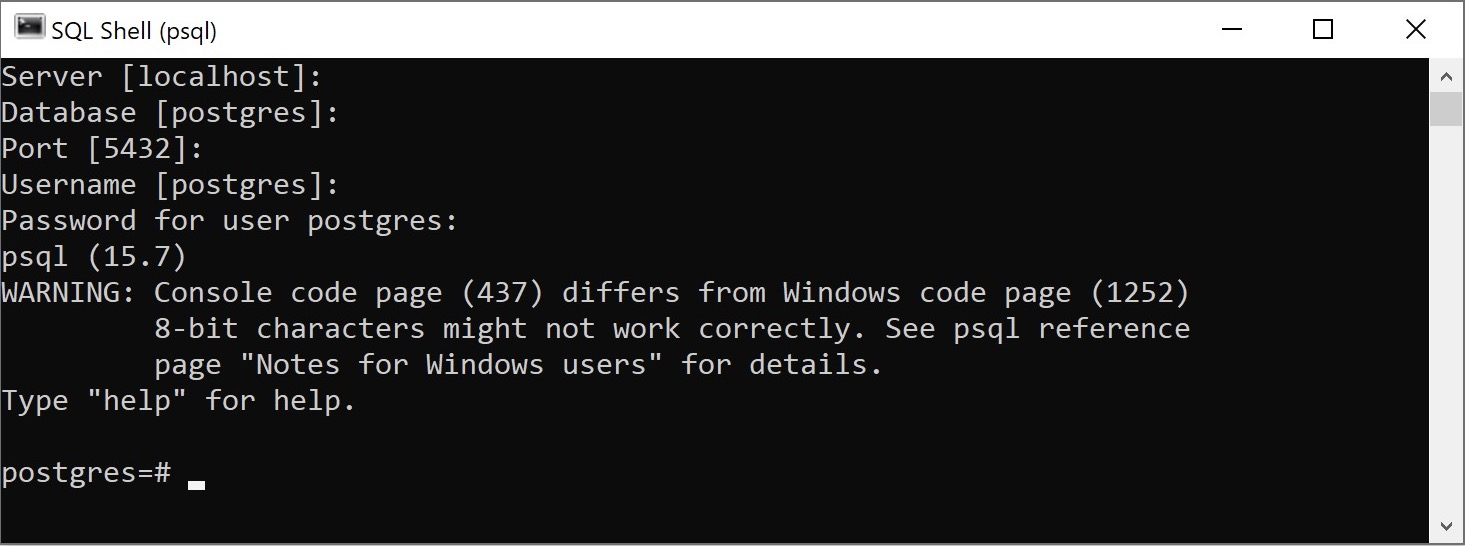
\includegraphics[width=.98\textwidth, trim={0mm 0mm 0mm 0.5mm},clip]{images/ch12/psqlconnect.jpg}};
  \drawshadow{image}
\end{tikzpicture}
\caption{psql မှ PostgreSQL ကို  စတင်ချိတ်ဆက်ပုံ} 
\label{fig:psqlconnect}
\end{figure}

\fEn{psql} ဖွင့်ပြီး စစချင်းမှာ ဒေတာဘေ့စ်နဲ့ ချိတ်ဆက်ဖို့ လိုအပ်တဲ့ အချက်အလက်တွေ ထည့်ပေးရပါမယ်။ ပုံ (\fRefNo{\ref{fig:psqlconnect}}) မှာ ကြည့်ပါ။ 
%
\begin{itemize}
\item \fEn{Server [localhost]:} (ချိတ်ဆက်မဲ့ ဆာဗာရဲ့ \fEn{Host Name/IP Address})
\item \fEn{Database [postgres]:} (ချိတ်ဆက်မဲ့ ဒေတာဘေ့စ်နံမည်)
\item \fEn{Port [5432]:} (\fEn{PostgreSQL port} နံပါတ်)
\item \fEn{Username [postgres]:} (ဒေတာဘေ့စ် ချိတ်ဆက်အသုံးပြုမဲ့ \fEn{user})
\item \fEn{Password for user postgres:} (ဒေတာဘေ့စ်ကို ချိတ်ဆက်အသုံးပြုမဲ့ \fEn{user} ရဲ့ \fEn{password})
\end{itemize}
%

လေးထောင့်ကွင်းထဲက \fEn{default} တန်ဖိုးတွေပါ။ တကူးတက ဘာမှမထည့်နေပဲ \fEn{Enter} နှိပ်ရင် အဲဒီတန်ဖိုးတွေ ထည့်တာနဲ့ တူတူပါပဲ။ စာမျက်နှာ \fRefNo{\pageref{apdx3}} နောက်ဆက်တွဲ (\fRefNo{\ref{apdx3}}) မှာ ဖော်ပြထားတဲ့အတိုင်း အင်စတောလ်လုပ်ထားတာဆိုရင် \fEn{password} တစ်ခုပဲ ထည့်ပေးဖို့လိုတယ်။ ကျန်တာက \fEn{default} အတိုင်းထားပြီး \fEn{Enter} နှိပ်သွားလို့ရတယ်။ \fEn{Password} က အင်စတောလ်လုပ်တုန်းက ပေးခဲ့တဲ့ \fEn{password} ကို ထည့်ပေးရမှာပါ။

\fEnBf{psql} ဆိုတာဘာလဲ။ \fEn{psql} ဟာ \fEn{PostgreSQL} ကို ချိတ်ဆက်အသုံးပြုဖို့ သုံးတဲ့ \fEn{command-line} ပရိုဂရမ်တစ်ခုပါ။ \fEn{Client} ပရိုဂရမ် အနေနဲ့ အသုံးပြုရတာပါ။ ဒေတာဘေ့စ် ချိတ်ဆက်ခြင်း၊ ဒေတာဘေ့စ်ဆီကို \fEn{SQL} ကွန်မန်းတွေ ပေးပို့လုပ်ဆောင်စေခြင်း၊ ဒေတာဘေ့စ် ပြန်ပို့ပေးတဲ့ ရလဒ်တွေပြပေးခြင်း၊ ဒေတာဘေ့စ် စီမံခန့်ခွဲခြင်း \fEn{(database administration)} စတဲ့ ကိစ္စတွေအတွက် အသုံးပြုနိုင်တယ်။ ရိုးရိုးရှင်းရှင်းပေမဲ့ အစွမ်းထက်တဲ့ \fEn{tool} တစ်ခုဖြစ်ပါတယ်။

\subsection*{ဒေတာဘေ့စ် အသစ်ဆောက်ခြင်း}
ဒေတာဘေ့စ် အသစ်တစ်ခု ဆောက်မယ်ဆိုရင် \fCode{CREATE DATABASE} \fEn{SQL} ကွန်မန်း သုံးပါတယ်။  
%
\begin{sql}
CREATE DATABASE ß\fEnEmp{database\_name}ß;
\end{sql}
%
\fEn{SQL language} ဟာ စာလုံး အကြီးအသေး မခွဲဘူး။ ဒီစာအုပ်မှာ \fEn{SQL keyword} တွေဆိုရင် အက္ခရာအကြီးနဲ့ ရေးပါမယ်။ \fEn{Database, table, column, function} စတာတွေရဲ့ နံမည် \fEn{(identifiers)} တွေက အက္ခရာအသေးနဲ့ ဖြစ်မယ်။
\fEn{student} ဒေတာဘေ့စ် အတွက် ဒီ \fEn{SQL} ကို
%
\begin{sql}
CREATE DATABASE students;
\end{sql}
%
\fEn{psql} ကနေ \fEn{run} ပေးပါ $\big\llbracket$ပုံ (\fRefNo{\ref{fig:createdb}})$\big\rrbracket$။ \fEn{SQL} စတိတ်မန့် တစ်ကြောင်း အဆုံးမှာ ဆီမီးကော်လံ \fEn{(\fCode{;})} ထည့်ပေးရပါမယ်။

\begin{figure}[tb!]
\begin{tikzpicture}
    \node[anchor=south west,inner sep=0] (image) at (0,0)
    {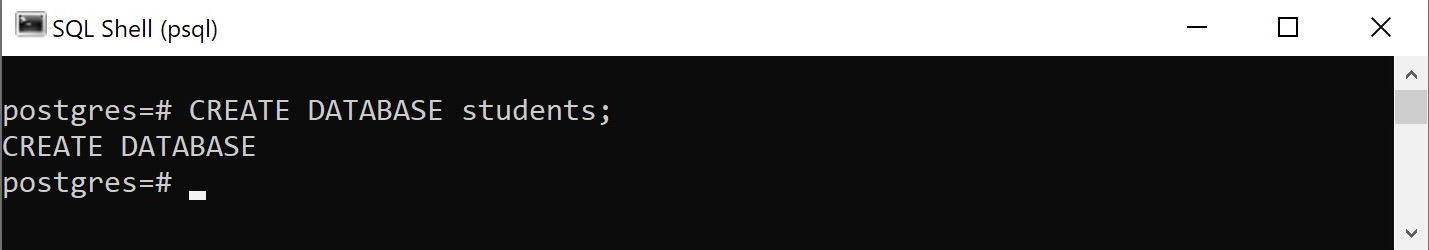
\includegraphics[width=.98\linewidth, trim={0mm, 0.5mm, 0.5mm, 0.5mm}, clip]{images/ch12/createdb.jpg}};
    \drawshadow{image}
\end{tikzpicture}
\caption{psql ကနေ ‘CREATE DATABASE’ SQL run တာ}
\label{fig:createdb}
\end{figure}

\fEn{psql} ကနေ \mintinline{text}|\l| (သို့) \mintinline{text}|\list| ကွန်မန်းနဲ့ \fEn{PostgreSQL} မှာ ရှိတဲ့ ဒေတာဘေ့စ်တွေကို ထုတ်ကြည့်နိုင်ပါတယ်။ ဒီလို \mintinline{text}|\| \fEn{(backslash)} နဲ့ စတဲ့ ကွန်မန်းတွေဟာ  \fEn{psql} သီးသန့်ဖြစ်တယ်။ \fEn{SQL} မဟုတ်တဲ့အတွက် \fEn{run} ရင် \fCode{;} မထည့်ရဘူး။ \mintinline{text}|\l| \fEn{run} လိုက်ရင် စာရင်းထဲမှာ \fEn{students} ဒေတာဘေ့စ် တွေ့ရမှာပါ $\big\llbracket$ပုံ (\fRefNo{\ref{fig:listdb}})$\big\rrbracket$။

\begin{figure}[htb!]
\begin{tikzpicture}
    \node[anchor=south west,inner sep=0] (image) at (0,0)
    {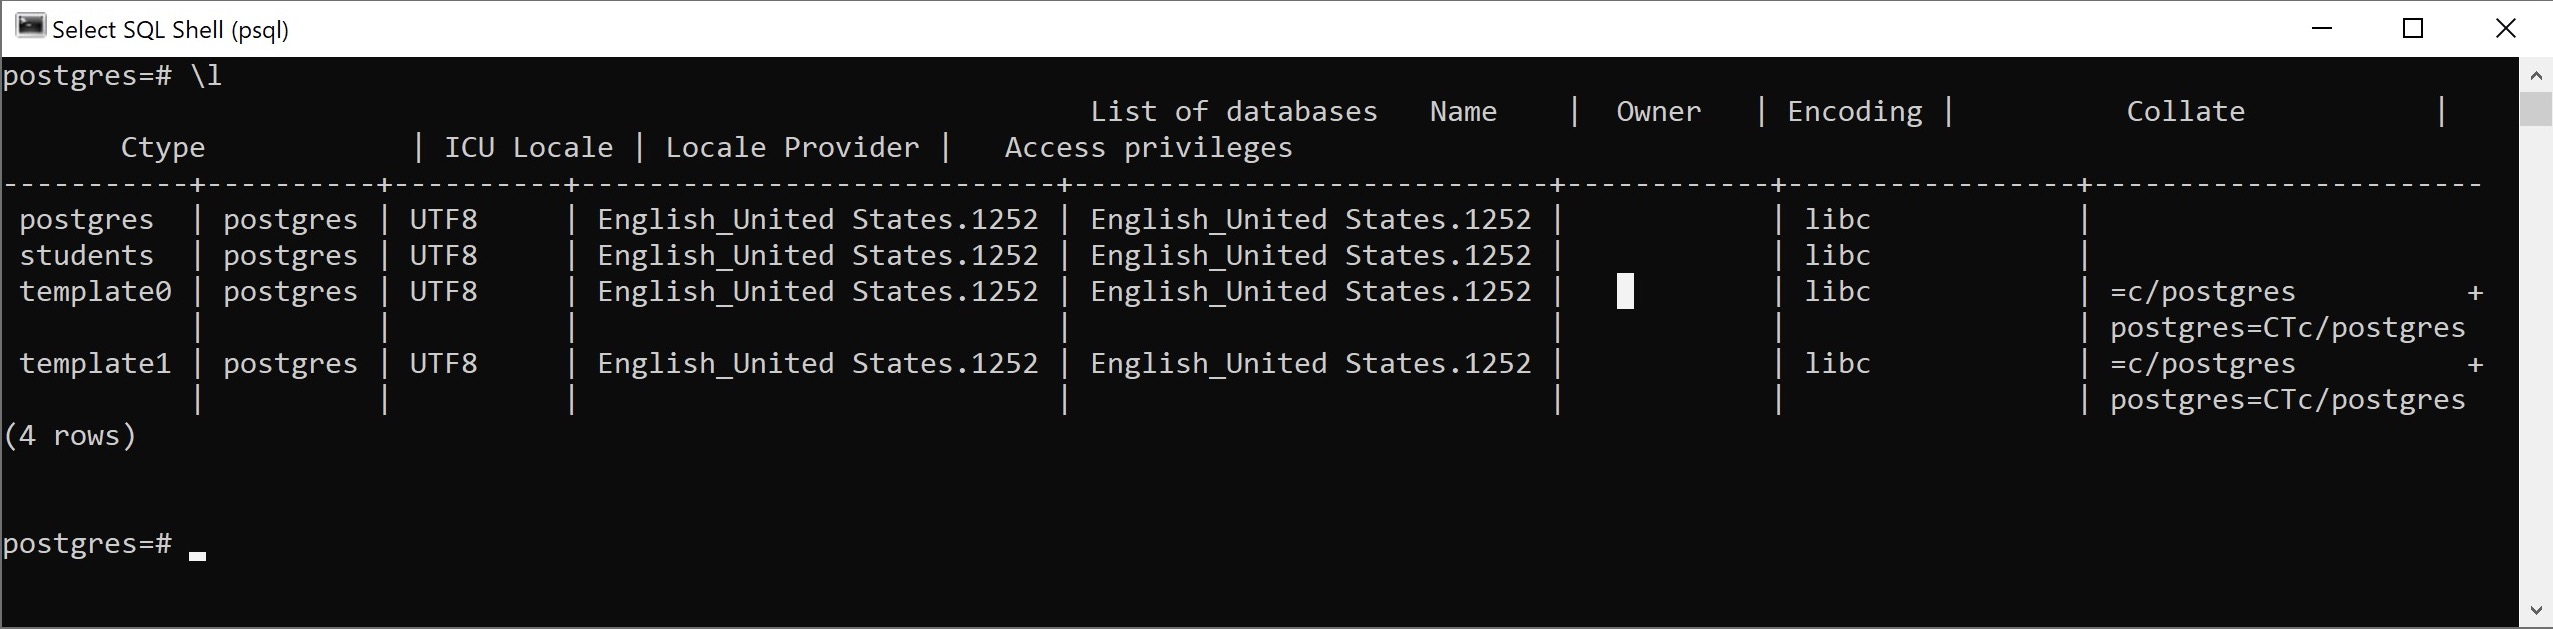
\includegraphics[width=.98\textwidth, trim={0mm 20mm 380mm 0.5mm},clip]{images/ch12/listdb.jpg}};
    \drawshadow{image}
\end{tikzpicture}
\caption{psql ကနေ ဒေတာဘေ့စ်တွေ list ထုတ်ကြည့်တာ}
\label{fig:listdb}
\end{figure}

\fEn{psql} မှာ ဒေတာဘေ့စ် ပြောင်းချိတ်မယ်ဆိုရင် \mintinline{text}|\c| (သို့) \mintinline{text}|\connect| နဲ့ ပြောင်းရပါမယ်။ \fEn{students} ဒေတာဘေ့စ်ကို အခုလို \fEn{connect} လုပ်ပါ
\begin{codetxt}
\c students
\end{codetxt}
\fEn{psql} က ဒီလို ပြပါလိမ့်မယ်
\begin{codetxt}
postgres=# \c students
You are now connected to database "students" as user "postgres".
students=#
\end{codetxt}

\begin{mytcbox}
\fEn{SQL} ကွန်မန်းကို \fEn{psql} က လုပ်ဆောင်ပေးတာ မဟုတ်ပါဘူး။ \fEn{psql} က \fEn{SQL} ကွန်မန်းကို ချိတ်ဆက်ထားတဲ့ ဒေတာဘေ့စ်ဆီ ပို့ပဲ ပို့ပေးတာ။ လက်ခံရရှိတဲ့ ဒေတာဘေ့စ်က အဲဒီ \fEn{SQL} ကို လုပ်ဆောင်ပေးတာပါ။ ဒီအချက်ကို ကွဲကွဲပြားပြား နားလည်ဖို့ လိုပါတယ်။
\end{mytcbox}

\subsection*{Table ဆောက်ခြင်း}
\fCode{CREATE TABLE} က \fEn{table} ဆောက်တဲ့ \fEn{SQL} ကွန်မန်းပါ။ \fEn{students} ဒေတာဘေ့စ်ထဲမှာ \fEn{student table} အောက်ပါအတိုင်း ဆောက်ပါမယ်
%
\begin{sql}
-- create a table named student 
CREATE TABLE student (
    id SERIAL PRIMARY KEY,
    name VARCHAR(100),
    age INT,
    grade VARCHAR(2)
);
\end{sql}
%  
\fEn{psql} မှာ \fEn{SQL} \fEn{run} ရင် လက်ရှိချိတ်ထားတဲ့ ဒေတာဘေ့စ်ကို အဲဒီ \fEn{SQL} ပေးပို့ လုပ်ဆောင်ခိုင်းပါတယ်။ အခုချိတ်ထားတာ \fEn{students} ဒေတာဘေ့စ်ဆိုတော့ \fEn{table} ကို အဲဒီ ဒေတာဘေ့စ်ထဲ ဆောက်ပေးသွားမှာပါ။ ဒီ \fEn{table} မှာ \fCode{id}\fEn{,} \fCode{name}\fEn{,} \fCode{age} နဲ့ \fCode{grade} \fEn{column} လေးခုရှိမယ်။ \fCode{--} ကို တစ်ကြောင်းတည်း ကွန်းမန့် အတွက် သုံးတယ်။ တစ်ကြောင်းထက်ပိုရင် \fCode{/*} နဲ့ ဖွင့် \fCode{*/} နဲ့ ပိတ် ရေးလေ့ရှိတယ်။ ဥပမာ
%
\begin{sql}
/* This is a
   multiline comment */
\end{sql}
%

\fEn{Column} တစ်ခုစီမှာ \fEn{data type} ရှိရပါမယ်။ \fCode{VARCHAR(100)} က အများဆုံး ကာရက်တာ အလုံးတစ်ရာ သိမ်းဆည်းနိုင်တယ်။ သိမ်းတဲ့ ကာရက်တာ အရေအတွက်ပေါ် မူတည်ပြီး နေရာယူတာ အနည်းအများ ကွာတယ်။ ငါခုသိမ်းရင် ငါးခုစာ၊ ဆယ်ခုသိမ်းရင် ဆယ်ခုစာပဲ နေရာကုန်မှာပါ။ အမြဲ အလုံး တစ်ရာစာ နေရာကုန်တာ မဟုတ်ဘူး။ \fCode{VARCHAR(2)} ဆိုရင် အများဆုံး  ကာရက်တာ နှစ်လုံး သိမ်းလို့ရမယ်။ \fEn{SQL} \fCode{VARCHAR} က \fEn{Python} \fCode{str} နဲ့ အလားတူတယ်။ \fCode{INT} ကတော့ \fEn{integer} ပါ။

\fCode{id} \fEn{column} က ထူးခြားပြီး နည်းနည်းပိုရှင်းပြဖို့ လိုတယ်။ \fCode{SERIAL} က \fEn{data type} အနေနဲ့ \fCode{INT} နဲ့ တူတူပဲ။ သူ့ရဲ့ ထူးခြားချက်က ဂဏန်းတွေကို အစဉ်အတိုင်း တစ်ခုပြီးတစ်ခု ထုတ်ပေးနိုင်တာပါ။ $1, 2, 3,\ldots$ စသည်ဖြင့်  နောက်ဆုံးတန်ဖိုးကို အလိုအလျောက် တစ်တိုးတိုးပြီး ထုတ်ပေးသွားမှာ ဖြစ်တယ်။ \fCode{id} \fEn{column} က \fEn{Primary Key} လည်းဖြစ်တယ်။ \fEn{Column} တစ်ခုကို \fEn{Primary Key} အဖြစ် ထားချင်ရင် \fCode{PRIMARY KEY} လို့ သတ်မှတ်ရပါမယ်။ \fEn{Primary Key} ဆိုရင် \fEn{column} တန်ဖိုး ထပ် \fEn{(duplicate)} လို့မရဘူး၊ \fEn{unique} ဖြစ်ရပါမယ်။ အခု သိပ်နားမလည်သေးရင်လည်း \fEn{table} မှာ ကျောင်းသား \fEn{record} တွေထည့်တာ ဆက်ကြည့်ရင် ကောင်းကောင်း နားလည်သွားမှာပါ။

\subsection*{\fSubSecCodeBf{INSERT}}
\fEn{Relational Data Model} အခြေခံတဲ့ \fEn{RDBMS} တွေဟာ ဒေတာတွေကို \fEn{table} ပုံစံနဲ့ သိမ်းဆည်းတယ်။ ကျောင်းသူ/သား တစ်ယောက်ချင်းစီအတွက် အချက်အလက်ကို \fEn{student table} မှာ  \fEn{row} တစ်ခုစီနဲ့ ထည့်သွင်း သိမ်းဆည်းပါမယ်။ \fEn{Row} ကို \fEn{record} လို့လည်း သုံးနှုန်းလေ့ရှိတယ်။ \fEn{Record} အသစ် ထည့်သွင်းမယ်ဆိုရင် \fEn{SQL} \fCode{INSERT} ကို သုံးရပါတယ်။

%
\begin{sql}
INSERT INTO student (name, age, grade) VALUES ('Amy', 20, 'A');
INSERT INTO student (name, age, grade) VALUES ('Kathy', 22, 'B');
INSERT INTO student (name, age, grade) VALUES ('Waiyan', 21, 'C');
\end{sql}
%

အေမီ၊ ကေသီ နဲ့ ဝေယံ ကျောင်းသား သုံးယောက်အတွက် \fEn{record} သုံးခု ထည့်သွင်းတာပါ။ \fEn{Column} နံမည်တွေ ဝိုက်ကွင်းထဲမှာ ထည့်ပြီး အဲ့ဒီ \fEn{column} တွေအတွက် တန်ဖိုးအသီးသီးကို အစဉ်အတိုင်း ထည့်ပေးရပါတယ်။ \fCode{age} နဲ့ \fCode{grade} ရှေ့နောက် ဖလှယ်လိုက်မယ်ဆိုရင် အခုလို
%
\begin{sql}
INSERT INTO student (name, grade, age) VALUES ('Amy', 'A',  20);
\end{sql}
%
\fEn{insert} လုပ်ရမှာပါ။

\fEn{student table} မှာ \fEn{column} က လေးခု ရှိတာပါ။ အခု \fCode{INSERT} တွေမှာကျတော့ သုံးခုပဲတွေ့ရပြီး \fCode{id} မပါဘူး။ ဘာကြောင့်ပါလဲ။ \fCode{INSERT} လုပ်တဲ့အခါ \fCode{SERIAL} \fEn{column} အတွက် တန်ဖိုးကို ဒေတာဘေ့စ်က အလိုအလျောက် ထည့်ပေးသွားတာ။ ကိုယ်တိုင်ထည့်ဖို့ မလိုဘူး။ ဒါကြောင့် \fCode{id} \fEn{column} ကို \fEnEmp{auto-incrementing} \fEn{primary key} \fEn{column} လို့ ခေါ်တယ်။ \fEn{Auto-increment} ဖြစ်ဖို့ အခြားနည်းလမ်းတွေလည်း ရှိပါတယ်။ \fCode{SERIAL} ကတော့ ဒီကိစ္စအတွက် လွယ်အောင် လုပ်ပေးထားတာပါ။ စောစောက \fCode{INSERT} သုံးကြောင်းကို \fEn{psql} မှာ \fEn{run} ပါ။ အေမီ၊ ကေသီ နဲ့ ဝေယံတို့အတွက် \fEn{record} အသီးသီးကို \fCode{id} နံပါတ် $1,2,3$ အစဉ်နဲ့ \fEn{student table} ထဲ ထည့်သွင်းသွားမှာဖြစ်တယ်။ နောက်ထပ် \fEn{record} တစ်ခု ထပ်ထည့်ရင် \fCode{id} နံပါတ် $4$ ဖြစ်မှာပါ။


\subsection*{\fSubSecCodeBf{SELECT}}
\fEn{Table} ဒေတာတွေ ထုတ်ယူကြည့်ဖို့ အသုံးပြုတဲ့ \fEn{SQL} ဖြစ်ပါတယ်။ \fEn{Student table} ထဲက \fEn{record} အားလုံးကို ကြည့်မယ်ဆို အခုလို 
%
\begin{sql}
SELECT id, name, age, grade FROM student;
\end{sql}
%
\fEn{Table} မှာ ရှိသမျှ \fEn{column} အကုန်လုံး ပါချင်ရင် \fCode{SELECT *} သုံးလို့လည်းရတယ်။ \fCode{SELECT *} ကို \fEn{‘Select All’} လို့ ဖတ်တယ်။
%
\begin{sql}
SELECT * FROM student;
\end{sql}
%

\begin{figure}[tbh!]
\begin{tikzpicture}
  \node[anchor=south west,inner sep=0] (image) at (0,0)
  {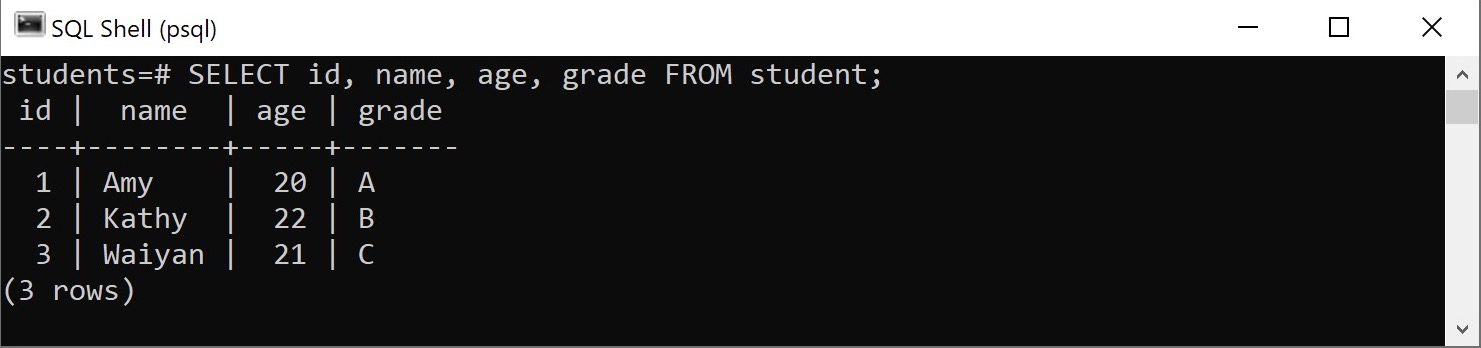
\includegraphics[width=.98\textwidth, trim={0mm 0.5mm 0.5mm 0.2mm}]{images/ch12/select.jpg}};
  \drawshadow{image}
\end{tikzpicture}
\caption{psql ကနေ select လုပ်တာ} 
\label{fig:selectstu}
\end{figure}

\fEn{Column} အကုန်မထုတ်ဘဲ ကိုယ်လိုချင်တာပဲ ရွေးပြီး \fEn{select} လုပ်ချင်လည်း ရတယ်။ အောက်ပါတို့ကို \fEn{psql} မှာ စမ်းကြည့်ပါ။
%
\begin{sql}
SELECT name, grade FROM student;
SELECT name, age, id FROM student;
\end{sql}
%
\subsection*{\fSubSecCodeBf{WHERE}}
\fEn{Grade A} ရတဲ့ ကျောင်းသားတွေကိုပဲ ရွေးထုတ်ကြည့်မယ် ဆိုပါစို့။ ဒီအတွက် \fEn{SQL} မှာ \fCode{WHERE} ရှိပါတယ်။ ဥပမာ
%
\begin{sql}
SELECT * FROM student WHERE grade = 'A';
\end{sql}
%
\fCode{WHERE} နောက်မှာ ဘူလီယန် အိပ်စ်ပရက်ရှင်တစ်ခု လိုက်ရပါမယ်။ \fCode{WHERE} ကွန်ဒီရှင် \fEn{(Condition)} လို့ခေါ်တယ်။ ရေးပုံရေးနည်း နည်းနည်းကွာပေမဲ့ \fEn{SQL} \fCode{WHERE} ကွန်ဒီရှင် က \fEn{Python} ဘူလီယန် အိပ်စ်ပရက်ရှင်နဲ့ သဘောတရားအားဖြင့် တူပါတယ်။ \fCode{grade = 'A'} က \fCode{grade} \fEn{column} တန်ဖိုး \fCode{'A'} နဲ့ ညီလား စစ်တာ။ ညီတဲ့ \fEn{record} တွေကိုပဲ \fCode{WHERE} က စစ်ထုတ်ပေးမှာပါ။ ဒါ့ကြောင့် အပေါ်က \fCode{select} က \fEn{record} တစ်ကြောင်းပဲ ထွက်မှာပါ။ အေမီတစ်ယောက်ပဲ \fEn{A} ရပါတယ်။ \fCode{WHERE} နဲ့ပါတ်သက်ပြီး လက်တွေ့စမ်းကြည့်ရအောင် အောက်ပါအတိုင်း ကျောင်းသား \fEn{record} လေးခု ထပ်ထည့်ပါမယ်။  
%
\begin{sql}
INSERT INTO student (name, age, grade) VALUES ('Sandy', 19, 'A');
INSERT INTO student (name, age, grade) VALUES ('Thida', 21, 'B');
INSERT INTO student (name, age, grade) VALUES ('Peter', 21, 'B');
INSERT INTO student (name, age, grade) VALUES ('Haymar', 18, NULL);
\end{sql}
%

\fEn{Grade A} သို့ \fEn{B} ရတဲ့ ကျောင်းသား \fEn{record} တွေ \fEn{select} လုပ်ဖို့ \fCode{OR} သုံးထားတာပါ။ \fEn{psql} မှာ စမ်းကြည့်ပါ။ \fEn{Amy, Kathy, Sandy, Thida, Peter} တို့ \fEn{A} သို့ \fEn{B} ရကြတယ်။
%
\begin{sql}
SELECT * FROM student WHERE grade = 'A' OR grade = 'B';
\end{sql}
\fEn{Grade A} သို့ \fEn{B} မရတဲ့ ကျောင်းသားတွေ ထုတ်ချင်ရင် \fCode{NOT} နဲ့ အခုလို ရတယ်
%
\begin{sql}
SELECT name FROM student WHERE NOT(grade = 'A' OR grade = 'B');
\end{sql}
ဝေယံ တစ်ယောက်ပဲ ရလဒ်မှာတွေ့ရမှာပါ။ ဟေမာ ဘာကြောင့် မပါရတာလဲ။ စဉ်းစားကြည့်ရင် သူမ \fEn{A} လည်းမရ၊ \fEn{B}  လည်းမရဘူး။ ဒါကြောင့်  ပါသင့်တယ် ယူဆကောင်း ယူဆနိုင်တယ်။ \fCode{NULL} ဟာ မရှိခြင်း၊ မသိခြင်း ကိုဖော်ပြဖို့ \fEn{SQL} မှာ အသုံးပြုတဲ့ \fEn{special value} တစ်ခု ဖြစ်ပါတယ်။ ဟေမာ့ \fEn{grade} က \fCode{NULL} ဖြစ်နေတယ်။ ဆိုလိုတာက သူ့ \fEn{grade} ကို မသိဘူး။ 

\fCode{NULL} နဲ့ အခြားတန်ဖိုးတစ်ခုခု ညီ/မညီ စစ်တဲ့အခါ ရလဒ်က \fCode{NULL} ပဲ ဖြစ်ပါတယ်။ အဓိပ္ပါယ်က ညီ/မညီ ‘မသိဘူး’ ဆိုတဲ့ အဓိပ္ပါယ်။ ဒါ့ကြောင့် ဘူလီယန် အိပ်စ်ပရက်ရှင် \fCode{'A' = NULL} ရဲ့ အဖြေ \fCode{NULL} ဖြစ်သလို \fCode{'A' <> NULL} ရဲ့ အဖြေလည်း \fCode{NULL} ပဲ ဖြစ်တယ်။ \fCode{<>} က မညီဘူးလား စစ်တာ၊ \fCode{=} နဲ့ ပြောင်းပြန်။ 

\fEn{Select} လုပ်တဲ့အခါ \fCode{WHERE} ကွန်ဒီရှင် \fEn{true} ဖြစ်တဲ့ \fEn{record} တွေကို ရွေးထုတ်ပေးတယ်။ \fCode{WHERE} ကွန်ဒီရှင် ရလဒ်တန်ဖိုး \fCode{NULL} ဖြစ်ရင် အဲဒီ \fEn{record} ကို ထုတ်ပေးမှာ မဟုတ်ဘူး။ စောစောက \fEn{select} ရလဒ်မှာ ဟေမာ ဘာ့ကြောင့်  မပါလဲ အောက်ပါအတိုင်း စဉ်းစားကြည့်နိုင်ပါတယ်%
%
\[
\begin{aligned}
         &\text{\fEn{WHERE NOT(\textit{NULL} = \`{}A\`{} OR \textit{NULL} = \`{}B\`{})}}\\
\implies &\text{\fEn{WHERE NOT(\textit{NULL} OR \textit{NULL})}}\\
\implies &\text{\fEn{WHERE NOT(\textit{NULL})}}\\
\implies &\text{\fEn{WHERE \textit{NULL}}}\\
\end{aligned}%
\]
\fEn{Grade C} မဟုတ်တဲ့ ကျောင်းသားတွေကို အောက်ပါအတိုင်း နည်းလမ်းနှစ်မျိုးနဲ့ \fEn{select} လုပ်ကြည့်ပါ။ အခုတစ်ခါလည်း ဟေမာ ရလဒ်မှာ မပါတာကို သတိပြုပါ။
%
\begin{sql}
SELECT * FROM student WHERE grade <> 'C';
\end{sql}
%
%
\begin{sql}
SELECT * FROM student WHERE NOT(grade = 'C');
\end{sql}
%
ဒီတစ်ခု ထပ်စမ်းကြည့်ပါ။ ရှင်းပြဖို့မလိုဘဲ အဓိပ္ပါယ် နားလည်မယ် ထင်ပါတယ်။
%
\begin{sql}
SELECT * FROM student WHERE grade = 'B' AND id <= 5;
\end{sql}
%

\fCode{NULL} ဟုတ်/မဟုတ် စစ်ချင်ရင် \fEn{SQL} မှာ \fCode{IS NULL} (သို့) \fCode{IS NOT NULL}  သုံးရပါတယ်။ \fCode{=} နဲ့ \fCode{<>} ကို သုံးလို့မရဘူး။ မှားယွင်း အသုံးပြုမိတတ်လို့ ဒီအချက်ကို အထူးဂရုပြုရပါမယ်။ \fEn{Grade} \fCode{NULL} ဖြစ်တဲ့ \fEn{record} တွေနဲ့ \fCode{NULL} မဟုတ်တဲ့ \fEn{record} တွေကို အခုလို ရွေးထုတ်နိုင်ပါတယ်။
%
\begin{sql}
SELECT * FROM student WHERE grade IS NULL;
SELECT * FROM student WHERE grade IS NOT NULL;
\end{sql}
%
\fEn{Grade} \fCode{NULL} ဖြစ်တာ ဟေမာတစ်ယောက်ပဲ ရှိတာမို့လို့ ပထမ \fEn{select} က \fEn{record} တစ်ကြောင်းပဲ ထွက်မှာပါ။ အောက်ပါအတိုင်း တစ်ဆင့်ချင်း စဉ်းစားကြည့်ပါ
\[
\begin{aligned}
    &\text{\fEn{WHERE grade IS \textit{NULL}}}\\
\implies &\text{\fEn{WHERE \textit{NULL} IS \textit{NULL}}}\\
\implies &\text{\fEn{WHERE TRUE}}\\
\end{aligned}
\]
ဒုတိယ \fEn{select} မှာ ကျတော့ ဘာကြောင့် ဟေမာ မပါလဲ။ ကျန်တဲ့သူတွေကရော ဘာကြောင့်ပါလဲ။ အောက်ပါအတိုင်း တစ်ဆင့်ချင်း စဉ်းစားကြည့်ပါ။ ဟေမာ့ \fEn{record} အတွက်%
%
\[
\begin{aligned}
    &\text{\fEn{WHERE grade IS NOT \textit{NULL}}}\\
\implies &\text{\fEn{WHERE \textit{NULL} IS NOT \textit{NULL}}}\\
\implies &\text{\fEn{WHERE FALSE}}\\
\end{aligned}
\]
\fEn{A} ရထားတဲ့ ကျောင်းသား \fEn{record} ဆိုရင် ဒီလို
\[ 
\begin{aligned}
    &\text{\fEn{WHERE grade IS NOT \textit{NULL}}}\\
\implies &\text{\fEn{WHERE \`{}A\`{} IS NOT \textit{NULL}}}\\
\implies &\text{\fEn{WHERE TRUE}}\\
\end{aligned}
\]
အခြား \fCode{NULL} မဟုတ်တဲ့ \fEn{grade} အားလုံးအတွက် အလားတူဖြစ်မယ်။ ဒါ့ကြောင့် ဒုတိယ \fEn{select} ရလဒ်မှာ ဟေမာကလွဲလို့ ကျန်တဲ့သူအားလုံး ပါလာတာဖြစ်တယ်။

\subsection*{\fSubSecCodeBf{ORDER BY}}
\fCode{ORDER BY} က \fEn{record} တွေကို \fEn{column} တန်ဖိုးပေါ် မူတည်ပြီး ‘အစဉ်အတိုင်းစီခြင်း’ \fEn{(sorting)} အတွက်ပါ။
%
\begin{sql}
SELECT * FROM student ORDER BY grade;
\end{sql}
%
\fEn{Grade} အလိုက် \fEn{order by} လုပ်ထားတာပါ။ ရလဒ်ကို ပုံ (\fRefNo{\ref{fig:orderbyasc}}) မှာ ကြည့်ပါ။ ကြီးစဉ်ငယ်လိုက် စီချင်ရင် \fCode{DESC} \fEn{(descending)} နဲ့ ရတယ်။
\begin{figure}[tbh!]
\begin{tikzpicture}
  \node[anchor=south west,inner sep=0] (image) at (0,0)
  {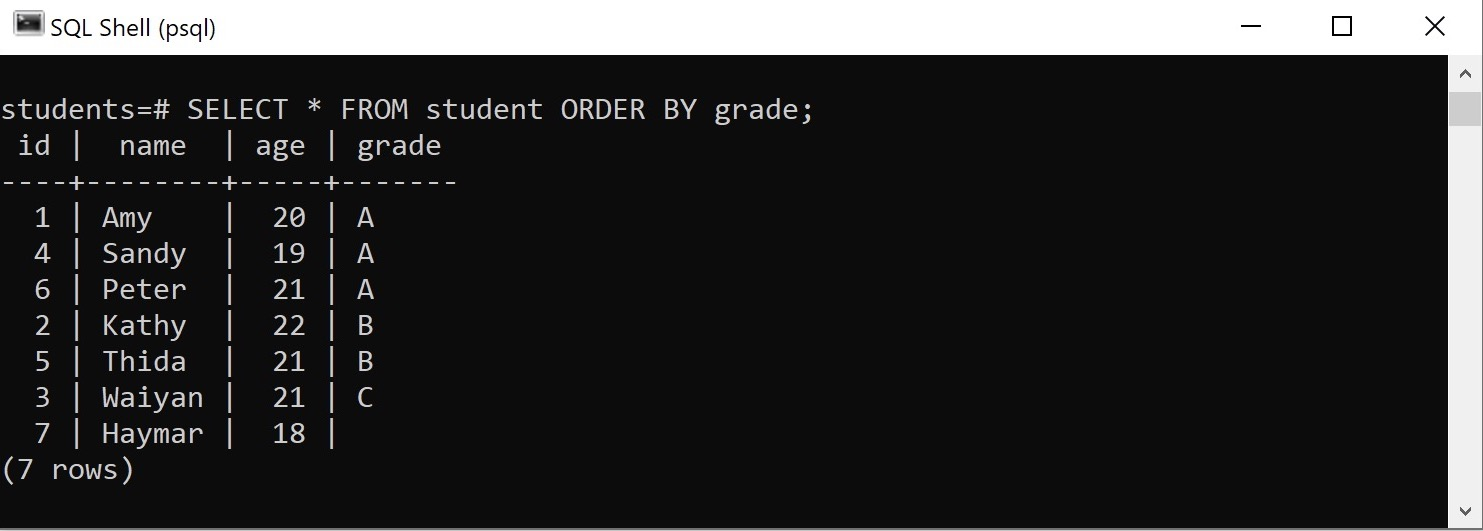
\includegraphics[width=.98\textwidth, trim={0mm 0.5mm 0.5mm 0.5mm},clip]{images/ch12/orderbyasc.jpg}};
  \drawshadow{image}
\end{tikzpicture}
\caption{order by နဲ့ grade အလိုက် စီထားတာ} 
\label{fig:orderbyasc}
\end{figure}
%
\begin{sql}
SELECT * FROM student ORDER BY grade DESC;
\end{sql}
%
သူ့ နဂို \fEn{default} ကတော့ \fCode{ASC} \fEn{(ascending)} ပါ။ 

\fEn{Column} တစ်ခုမကနဲ့  စီချင်လည်း ရတယ်။ \fCode{ORDER BY} နောက်မှာ \fEn{sort} လုပ်ရမဲ့ \fEn{column} တွေ ထည့်ပေးရုံပဲ။ \fEn{Age} နဲ့ \fEn{grade} တွဲရက် \fEn{sort} လုပ်မယ်ဆိုရင်
%
\begin{sql}
SELECT * FROM student ORDER BY age, grade;
\end{sql}
%
\fEn{psql} ရလဒ်မှာ အောက်ပါအတိုင်း တွေ့ရမှာပါ။ \fEn{Thida, Peter, Waiyan} တို့ကို သေချာ ဂရုပြုကြည့်ပါ။ \fEn{Age} တူရင် \fEn{grade B} ရတဲ့သူက အရင်လာတာကို တွေ့ရပါမယ်။ \fEn{Grade C} က နောက်မှာပါ။
\begin{vbtm}
ß\fEnBf{Output:}ß
 id |  name  | age | grade
----+--------+-----+-------
  7 | Haymar |  18 |
  4 | Sandy  |  19 | A
  1 | Amy    |  20 | A
  5 | Thida  |  21 | B
  6 | Peter  |  21 | B
  3 | Waiyan |  21 | C
  2 | Kathy  |  22 | B
(7 rows)
\end{vbtm}
\fEn{Name} ထပ်ထည့်ကြည့်ပါ။  \fEn{Peter} က \fEn{Thida} ရဲ့ ရှေ့ရောက်သွားတာကလွဲလို့ ခုနက စီထားတာနဲ့ အားလုံးတူပါမယ်။
%
\begin{sql}
SELECT * FROM student ORDER BY age, grade, name;
\end{sql}
%

\fEn{Age} နဲ့ \fEn{grade} ကို ရှေ့‌နောက် ပြောင်းကြည့်ပါ။ 
%
\begin{sql}
SELECT * FROM student ORDER BY grade, age;
\end{sql}
%
\fEn{Grade} \fEn{A, B, C} အစဉ်အတိုင်း ဖြစ်မယ်။ \fEn{Grade} တူရင်တော့ \fEn{age} ငယ်တဲ့ \fEn{record} က ရှေ့ရောက်ပါတယ်။ အခုလို စီသွားမှာပါ
%
\begin{vbtm}
ß\fEnBf{Output:}ß
 id |  name  | age | grade
----+--------+-----+-------
  4 | Sandy  |  19 | A
  1 | Amy    |  20 | A
  5 | Thida  |  21 | B
  6 | Peter  |  21 | B
  2 | Kathy  |  22 | B
  3 | Waiyan |  21 | C
  7 | Haymar |  18 |
(7 rows)
\end{vbtm}
%

\fEn{Grade} ကို \fCode{DESC} နဲ့ \fEn{age} ကို \fCode{ASC} ထားကြည့်ပါ။ ခုနကဟာနဲ့ ဘာကွာခြားလဲ သေချာဂရုပြု လေ့လာကြည့်ပါ။
%
\begin{sql}
SELECT * FROM student ORDER BY grade DESC, age ASC;
\end{sql}
%
\begin{vbtm}
ß\fEnBf{Output:}ß
 id |  name  | age | grade
----+--------+-----+-------
  7 | Haymar |  18 |
  3 | Waiyan |  21 | C
  6 | Peter  |  21 | B
  5 | Thida  |  21 | B
  2 | Kathy  |  22 | B
  4 | Sandy  |  19 | A
  1 | Amy    |  20 | A
(7 rows)
\end{vbtm}

\fCode{ORDER BY} နဲ့ စီတဲ့အခါ \fCode{ORDER BY} နောက်မှာ \fEn{list} လုပ်ထားတဲ့ \fEn{column} အစီအစဉ်နဲ့ \fCode{ASC}\fEn{,} \fCode{DESC} တို့ကို လိုသလို အသုံးပြုပြီး လိုချင်တဲ့အတိုင်း ရအောင် \fEn{sort} လုပ်လို့ရပါတယ်။ ပရိုဂရမ်းမင်းမှာရော ဒေတာဘေ့စ်ပိုင်းမှာပါ \fEn{sorting} စီခြင်းဟာ အရေးကြီးတာကြောင့် ကျွမ်းကျင်အောင် လုပ်ထားသင့်ပါတယ်။


\subsection*{\fSubSecCodeBf{UPDATE}}
\fEn{Table record} တွေ \fEn{update} လုပ်ဖို့ အသုံးပြုတဲ့ \fEn{SQL} စတိတ်မန့် ဖြစ်ပါတယ်။ \fCode{id} နံပါတ် \fEn{7} နဲ့ \fEn{record} ရဲ့ \fEn{grade} နဲ့ \fEn{age} ကို \fEn{update} လုပ်မယ်ဆိုရင် ဒီလို
%
\begin{sql}
UPDATE student SET grade = 'A', age = 19 WHERE id = 7;
\end{sql}
%
\fCode{WHERE} ပါရင် \fCode{WHERE} ကွန်ဒီရှင်နဲ့ ကိုက်ညီတဲ့ \fEn{record} ကိုပဲ \fEn{update} လုပ်တယ်။ အခု \fEn{update} စတိတ်မန့်က \fCode{id} \fEn{7} နဲ့ က ဟေမာ့ \fEn{record} တစ်ခုကိုပဲ \fEn{update} လုပ်မှာပါ။ အကယ်၍ \fCode{WHERE} မပါခဲ့ရင် \fEn{table} မှာရှိတဲ့ \fEn{record} တွေ အကုန်လုံးကို \fEn{update} လုပ် သွားလိမ့်မယ်။

%
\begin{sql}
UPDATE student SET grade = 'A+' WHERE id IN (1, 4, 6);
\end{sql}
%
\fCode{id} နံပါတ်က $(1,4,6)$ ထဲမှာပါရင် \fEn{grade} ကို \fEn{A+} \fEn{update} လုပ်ထားတာပါ။ \fCode{WHERE} ကွန်ဒီရှင်မှာ \fCode{IN}  အော်ပရိတ်တာ သုံးထားတယ်။ \fEn{Column} တစ်ခုရဲ့ တန်ဖိုးဟာ \fEn{list} လုပ်ထားတဲ့ တန်ဖိုးတွေထဲမှာ ပါ/မပါ စစ်ချင်ရင် \fCode{IN} သုံးပါတယ်။ \fEn{Update} လုပ်ထားတဲ့ \fEn{record} တွေကို \fEn{select} လုပ်ကြည့်ပါ။ 
%
\begin{sql}
SELECT * FROM student WHERE id IN (1, 4, 6, 7);
\end{sql}
%
ပုံ (\fRefNo{\ref{fig:afterupdate}}) မှာလို တွေ့ရပါမယ်။

\begin{figure}[tbh!]
\begin{tikzpicture}
  \node[anchor=south west,inner sep=0] (image) at (0,0)
  {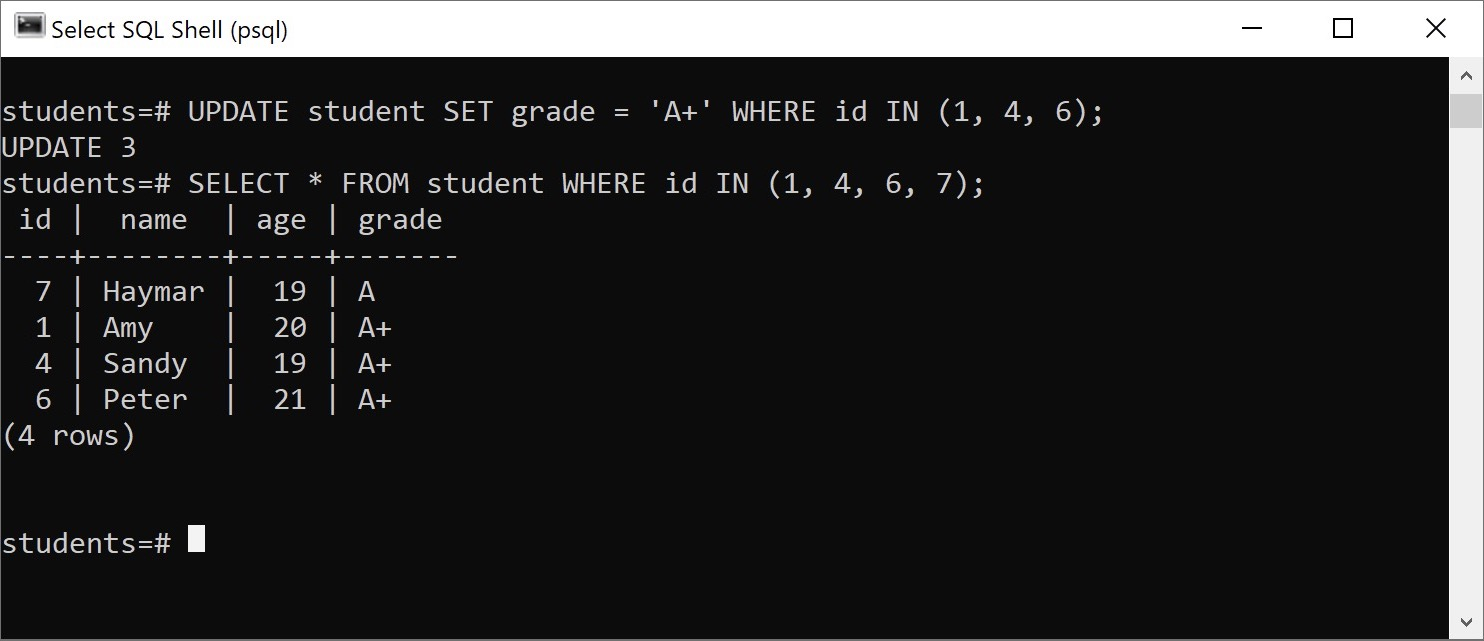
\includegraphics[width=.98\textwidth, trim={0mm 50mm 0.5mm 0.5mm},clip]{images/ch12/afterupdate.jpg}};
  \drawshadow{image}
\end{tikzpicture}
\caption{record တချို့ကို update လုပ်ပြီးနောက် select ပြန်လုပ်ကြည့်တာ} 
\label{fig:afterupdate}
\end{figure}

\subsection*{\fSubSecCodeBf{DELETE}}
\fEn{Table row} တွေ ဖျက်ဖို့ အသုံးပြုတဲ့ စတိတ်မန့် ဖြစ်ပါတယ်။ \fEn{Student table} ထဲက \fEn{record} အားလုံး ဖျက်မယ်ဆိုရင် အခုလို ဖျက်ရမှာပါ
%
\begin{sql}
DELETE FROM students;
\end{sql}
%
\fEn{Development/testing} ဒေတာဘေ့စ်မှာ \fEn{table} ဒေတာ အကုန်ဖျက်ပြီး အစမ်းဒေတာ \fEn{(test data)} ပြန်ထည့်ဖို့ ဒီလို လုပ်ရလေ့ရှိပေမဲ့ တကယ်သုံးနေတဲ့ \fEn{production} ဒေတာဘေ့စ်မှာတော့ \fEn{table} ဒေတာ အကုန်ဖျက်ပစ်ရမဲ့ အခြေအနေဆိုတာ ကြုံတောင့်ကြုံခဲပါပဲ။ ဖျက်ရမဲ့ \fEn{record} ကို \fCode{WHERE} နဲ့ရွေး ဖျက်တာက ပိုပြီး သဘာဝကျပါတယ်။ ဝေယံ ကျောင်းထွက်သွားလို့ သူ့ \fEn{record} ကို သိမ်းထားဖို့ မလိုတော့ဘူး ဆိုပါစို့၊ အခုလို \fEn{delete} လုပ်နိုင်ပါတယ် 
%
\begin{sql}
DELETE FROM student WHERE id = 3; -- id 3 is Waiyan
\end{sql}
%


\section{Table Relationships}
ဒေတာဘေ့စ် တစ်ခုမှာ \fEn{table} တစ်ခုမက \fEn{(multiple tables)} ပါဝင် ဖွဲ့စည်းထားလေ့ ရှိတယ်။ \fEn{Table} တွေနဲ့ ၎င်းတို့ကြား \fEnEmp{relationship} ဟာ \fEn{Relational Data Model} ရဲ့ အဓိကကျတဲ့ သဘောတရားဖြစ်တယ်။ သက်ဆိုင်\allowbreak ရာ \fEn{table} အသီးသီးမှာ အချက်အလက်တွေ စုစည်းသိမ်းဆည်းပုံ သိမ်းဆည်းနည်း စနစ်ကို လေ့လာကြရအောင်။ 

ဘဏ်တစ်ခုကို စိတ်ကူးကြည့်ပါ။ ဘဏ်အကောင့်၊ အကောင့်ပိုင်ရှင်နဲ့ ငွေဝင်ငွေထွက် စာရင်း အချက်\allowbreak အလက်တွေ သိမ်းဆည်းမယ် ဆိုပါစို့။ \fEn{Table} တစ်ခုတည်းနဲ့ အားလုံးသိမ်းလို့ ရပေမဲ့ \fEn{Relational Data Model} အရ \fEn{table} သုံးခုခွဲပြီး သီးခြားစီသိမ်းတာ ပိုကောင်းပါတယ်။  အကောင့်ပိုင်ရှင်နဲ့ သက်ဆိုင်တဲ့ အချက်အလက်တွေအတွက် \fEn{table} တစ်ခု ရှိပါမယ်။
%
\begin{sql}
CREATE TABLE account_holder (
    holder_id SERIAL PRIMARY KEY,
    fname VARCHAR(50),
    lname VARCHAR(50),
    dob DATE,
    address TEXT
);
\end{sql}
%
အခု \fEn{table} တွေကို ဒေတာဘေ့စ် အသစ်တစ်ခုထဲမှာထားတာ ပိုသင့်တော်မယ်။ (ကျောင်းသား ကိစ္စနဲ့ဆိုင်တဲ့ \fEn{table} တွေကို \fEn{students} ဒေတာဘေ့စ်၊ ဘဏ်နဲ့သက်ဆိုင်တာကို \fEn{bank} ဒေတာဘေ့စ် သတ်သတ်စီခွဲထားရင် ပိုပြီး စနစ်ကျတာကြောင့်ပါ။ အစမ်းလေ့လာတာမို့ သိပ်တော့ အရေးမကြီးပါ)။ \fEn{psql} မှာ အောက်ပါအတိုင်း တစ်ကြောင်းချင်း \fEn{run} ပါ
\begin{vbtm}
\c postgres
CREATE DATABASAE bank;
\c bank
\end{vbtm}
ပြီးတော့မှ \fCode{account\_holder} \fEn{table} အတွက် အပေါ်က \fCode{CREATE TABLE} ကို ဆက် \fEn{run} ပါ။ အခုချိတ်ထားတာက \fCode{bank} ဒေတာဘေ့စ် (\mintinline{text}|\c bank| \fEn{run} ထားတာ သတိပြုပါ)၊ ဆိုတော့ \fEn{table} က အဲဒီထဲမှာ ဆောက်မှာပါ။

အကောင့်နဲ့ သက်ဆိုင်တဲ့ အချက်အလက်တွေအတွက် \fEn{table} တစ်ခု ထပ်ဆောက်ပါမယ်။ (အခု \fEn{table} နှစ်ခုကို အရင်ကြည့်ရအောင်၊ ငွေဝင်ငွေထွက် စာရင်းနဲ့ ဆိုင်တဲ့ တတိယ \fEn{table} ကို နောက်ပိုင်းမှာ တွေ့ရမှာပါ)။ 
%
\begin{sql}
CREATE TABLE account (
    acc_id SERIAL PRIMARY KEY,
    /* ß\fMM{အခု}ß holder_id ß\fMM{က}ß account_holder ß\fEn{table} \fMM{ရဲ့}ß holder_id ß\fMM{ကို}ß 
    ß\fEn{reference} \fMM{လုပ်ထားတယ်}ß */ 
    holder_id INT REFERENCES account_holder(holder_id),
    acc_no VARCHAR(20) UNIQUE,
    acc_type VARCHAR(20),
    balance NUMERIC(12, 2) DEFAULT 0.00
);
\end{sql}
%

\fCode{account} \fEn{table} မှာ \fCode{holder\_id} \fEn{column} က \fCode{account\_holder} \fEn{table} ရဲ့ \fCode{holder\_id} \fEn{column} ကို ရည်ညွှန်းထားပါတယ်။ အကောင့်နဲ့ အကောင့် ပိုင်ရှင် အချက်အလက်တွေကို ဒီ \fEn{table} နှစ်ခုမှာ ဘယ်လို ဆက်စပ် သိမ်းဆည်းလဲ နားလည်အောင် နမူနာ \fEn{record} အနည်းငယ်ထည့်ပြီး ရှင်းပြပါမယ်။ အောက်ပါအတိုင်း \fEn{insert} လုပ်ပါ။
%
\begin{sql}
INSERT INTO account_holder (fname, lname, dob, address)
VALUES 
('Amy', 'Moe', '1985-02-15', '123 Main St, Sanchaung'),
('Sandy', 'Soe', '1990-06-23', '456 Oak St, Kamayaut');
\end{sql}
%
\fEn{Insert} လုပ်ပြီးရင် အေမီနဲ့ စန္ဒီ့ \fCode{holder\_id} နံပါတ်က $1$ နဲ့ $2$ အသီးသီး ဖြစ်မယ်။ အေမီဖွင့်ထားတဲ့ အကောင့်နှစ်ခုနဲ့ စန္ဒီရဲ့ အကောင့်တစ်ခုကို အောက်ပါအတိုင်း \fCode{account} \fEn{table} မှာ သိမ်းနိုင်ပါတယ်။ \fCode{holder\_id} $1$ နဲ့ $2$ ကို အထူး ဂရုပြုပါ။
%
\begin{sql}
INSERT INTO account (holder_id, acc_no, acc_type, balance)
VALUES 
(1, '0086-6002-1111', 'Savings', 500000.00),
(1, '0088-6005-1122', 'Current', 800000.00),
(2, '0086-6002-3311', 'Savings', 400000.00);
\end{sql}
%
ဒီ \fEn{table} မှာ ကြည့်ရင် အကောင့်ပိုင်ရှင် အသေးစိတ်အချက်အလက်ကို မတွေ့ရပါဘူး။ အကောင့် \fEn{record} တစ်ခုစီအတွက်  ပိုင်ရှင်ရဲ့ \fCode{holder\_id} ကိုပဲ တွေ့ရမှာပါ။ ဒီ \fCode{holder\_id} ဟာ \fCode{account\_holder} \fEn{table} ထဲက \fEn{record} တစ်ခုရဲ့ \fCode{holder\_id} ကို ရည်ညွှန်းရပါမယ်။ 

ပထမ အကောင့်နှစ်ခု \fCode{holder\_id} က $1$ ဖြစ်တယ်။ \fCode{account\_holder} \fEn{table} မှာပြန်ကြည့်ရင် \fCode{holder\_id} $1$ က အေမီ။ ဒါကြောင့် ဒီအကောင့်နှစ်ခုဟာ အေမီ့ရဲ့ အကောင့်ဖြစ်တယ်။ ထိုနည်းတူစွာ \fCode{holder\_id} $2$ က စန္ဒီဖြစ်တဲ့အတွက် တတိယအကောင့်ဟာ သူမရဲ့ အကောင့်ဖြစ်တယ်လို့ သိနိုင်ပါတယ်။ အခု ဖော်ပြခဲ့သလို အချက်အလက် သိမ်းဆည်းပုံ နည်းစနစ်ဟာ \fEn{Relational Model} ရဲ့ အဓိကကျတဲ့ အခြေခံ သဘောတရားလို့ ဆိုရမှာပါ။

\subsection*{Table \fSubSecCodeBf{JOIN}}
\fEn{Table} နှစ်ခုကို ပေါင်းစပ်ကြည့်ရင် အကောင့်ရော အကောင့်ပိုင်ရှင် အချက်အလက်ကိုပါ အပြည့်အစုံ သိနိုင်မှာပါ။ ဥပမာ အခုလို \fEn{select} လုပ်ကြည့်ရင် အေမီနဲ့ သူမ၏အကောင့် အသေးစိတ် အချက်အလက်တွေကို တွေ့ရပါမယ်
%
\begin{sql}
SELECT * FROM account_holder WHERE holder_id = 1;
SELECT * FROM account WHERE holder_id = 1;
\end{sql}
%
\begin{vbtm}
ß\fEnBf{Output:}ß
 holder_id | fname | lname |    dob     |        address
-----------+-------+-------+------------+------------------------
         1 | Amy   | Moe   | 1985-02-15 | 123 Main St, Sanchaung
(1 row)


 acc_id | holder_id |     acc_no     | acc_type |  balance
--------+-----------+----------------+----------+-----------
      1 |         1 | 0086-6002-1111 | Savings  | 500000.00
      2 |         1 | 0088-6005-1122 | Current  | 800000.00
(2 rows)
\end{vbtm}

\fEn{Table} နှစ်ခု ချိတ်ဆက်ပြီး အကောင့်နဲ့ အကောင့်ပိုင်ရှင် တစ်ဆက်တည်း ထုတ်ကြည့်မယ် ဆိုရင်တော့ ဒီအတွက် \fEn{SQL} \fCode{JOIN} ရှိပါတယ်။
%
\begin{sql}
SELECT * FROM account_holder JOIN account
ON account_holder.holder_id = account.holder_id;
\end{sql}
%
\fEn{Psql} မှာ စမ်းကြည့်ရင် အခုလို ရမှာပါ

\begin{figure}[H]
\begin{tikzpicture}
  \node[anchor=south west,inner sep=0] (image) at (0,0)
  {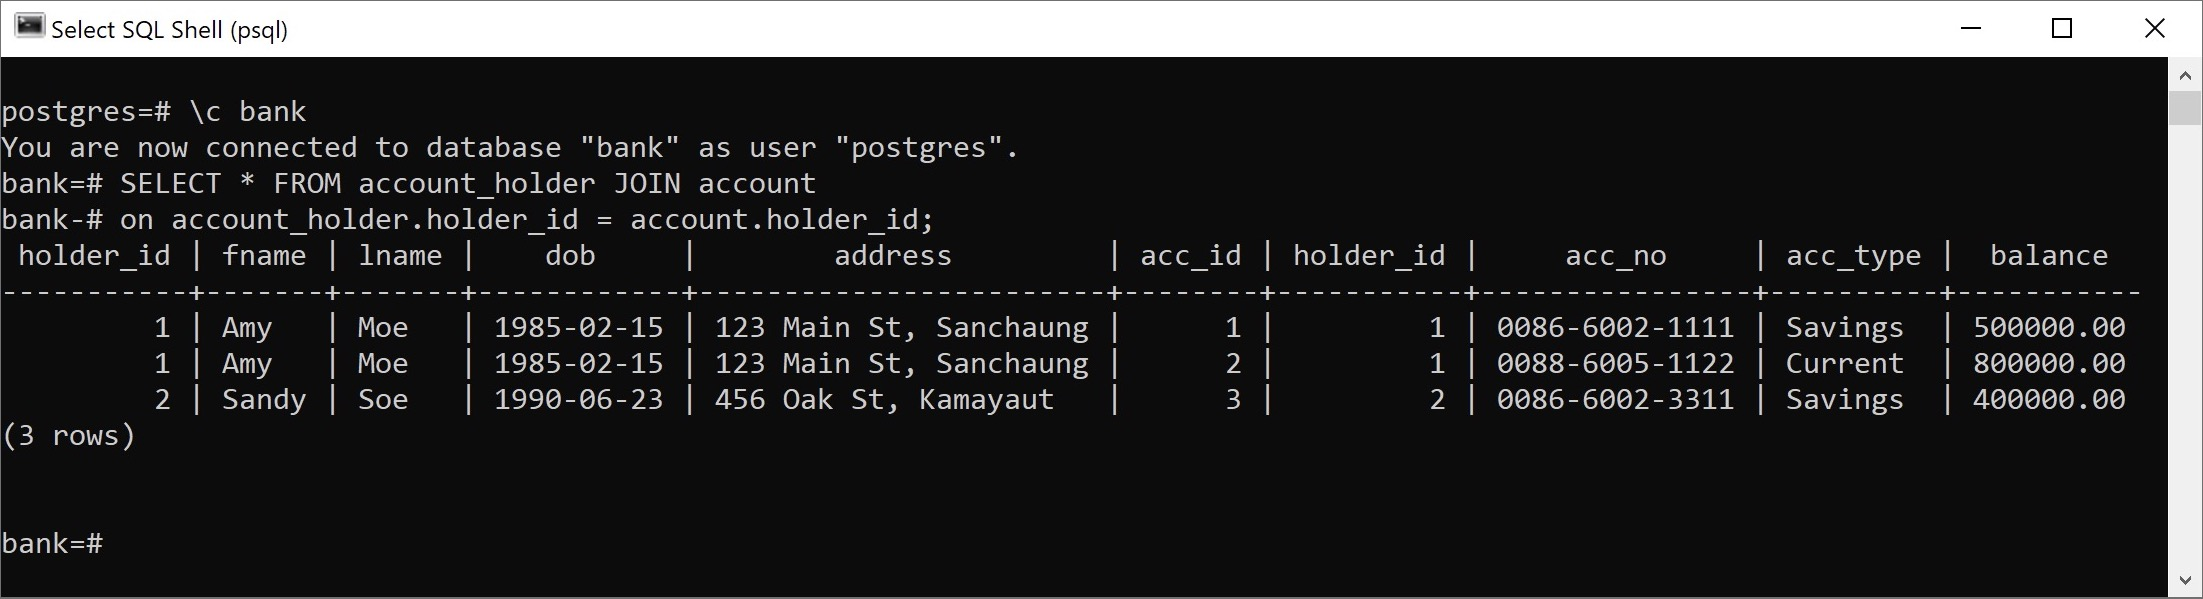
\includegraphics[width=1.13\textwidth, trim={0mm 50mm 0mm 0.5mm},clip]{images/ch12/join.jpg}};
  \drawshadow{image}
\end{tikzpicture}
\caption{table နှစ်ခု join ပြီး select လုပ်ထားတာ} 
\label{fig:join}
\end{figure}
\fCode{account\_holder} \fEn{table} ရဲ့ \fCode{holder\_id} နဲ့  \fCode{account} \fEn{table} ရဲ့ \fCode{holder\_id} တူရင် \fCode{JOIN} က \fEn{record} တွေကို တွဲဆက်ပေးတာ တွေ့ရမှာပါ။ တွဲဆက်ပေးရမဲ့ ကွန်ဒီရှင်ကို \fCode{ON} နောက်မှာ အခုလို ထည့်ပေးထားတယ်
%
\begin{sql}
ON account_holder.holder_id = account.holder_id;
\end{sql}
%
အောက်မှာ နောက်ထပ် ပုံစံတစ်မျိုး ရေးထားတာကို ကြည့်ပါ။ \fCode{account\_holder} \fEn{table} ကို \fCode{t1} ၊ \fCode{account} ကို \fCode{t2} နဲ့ ရည်ညွှန်းပါတယ်။ \fEn{Alias} လုပ်တာလို့ ခေါ်ပါတယ်။
%
\begin{sql}
SELECT 
    t1.*,
    t2.* 
FROM account_holder t1 JOIN account t2
    ON t1.holder_id = t2.holder_id;
\end{sql}
%
\fEn{Table} နှစ်ခုကနေ လိုချင်တဲ့ \fEn{column} ကိုပဲ ရွေးထုတ်လည်း ရတယ်။ ဥပမာ
%
\begin{sql}
SELECT 
    t2.*,
    t1.fname,
    t1.lname
FROM account_holder t1 JOIN account t2
    ON t1.holder_id = t2.holder_id;
\end{sql}
%

\subsection*{Referential Integrity}
\fEn{Relational Model} ဟာ \fEnEmp{referential integrity} ကို မပျက်ယွင်းအောင် အလေးအနက်ထား  ထိန်းသိမ်းပေးပါတယ်။ \fEn{Record} တစ်ခုကို ဖျက်တဲ့အခါ အဲဒီဖျက်လိုက်တဲ့ \fEn{record} ကို အခြား \fEn{table} မှာရှိတဲ့ \fEn{record} တွေက ရည်ညွှန်းထားမယ်ဆိုရင် ပြဿနာရှိတယ်။ ဥပမာ \fCode{account\_holder} \fEn{table} မှာ အကောင့်ပိုင်ရှင် အေမီ့ \fEn{record} ကို ဖျက်လိုက်တယ် ဆိုပါစို့။ ဒီလိုဆိုရင် \fCode{account} \fEn{table} ထဲက \fCode{holer\_id} $1$ နဲ့ အကောင့်နှစ်ခု ရည်ညွှန်းထားတဲ့ အကောင့်ပိုင်ရှင် \fEn{record} ရှိမှာ မဟုတ်တော့ဘူး။ ဒါဟာ \fEn{referential integrity} ကို ချိုးဖောက်တာ ဖြစ်တဲ့အတွက် \fEn{Relational Model} က အဲဒီလို ဖျက်ခွင့်ပေးမှာ မဟုတ်ပါဘူး။ \fEn{Record} တစ်ခုကို အခြား \fEn{record} တွေက \fEn{reference} လုပ်ထားတာ ရှိနေသ၍ \fEn{Relational Model} က အဲ့ဒီ \fEn{record} ပေးမဖျက်ဘူး။ အခုလို စမ်းပြီး ဖျက်ကြည့်ပါ။ 
%
\begin{figure}[tbh!]
\begin{tikzpicture}
  \node[anchor=south west,inner sep=0] (image) at (0,0)
  {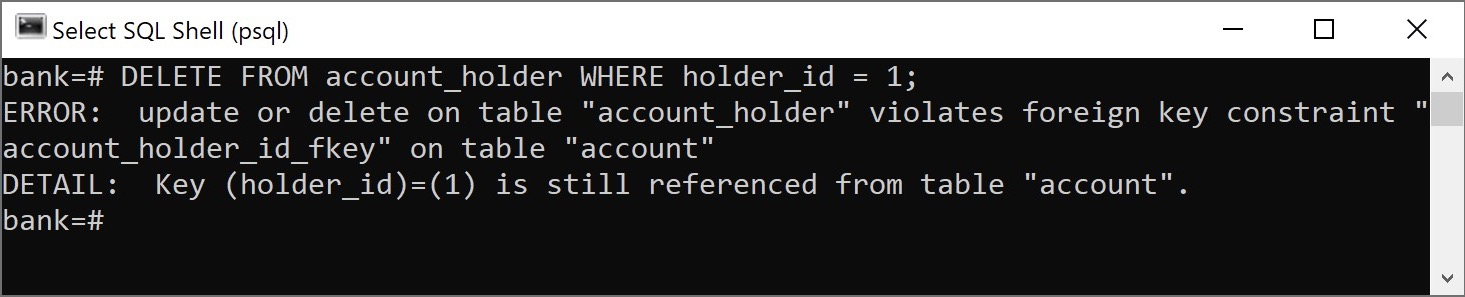
\includegraphics[width=.98\textwidth, trim={0.5mm 0mm 0mm 0.8mm},clip]{images/ch12/ref_integrity.jpg}};
  \drawshadow{image}
\end{tikzpicture}
\caption{referential integrity အရ ပေးမဖျက်တာ} 
\label{fig:ref_integrity}
\end{figure}%
ဖျက်ခွင့်မပေးတာကို တွေ့ရပါလိမ့်မယ်။

\fCode{holer\_id} $1$ နဲ့ \fEn{record} ကို ဖျက်ချင်ရင် ၎င်းကို ရည်ညွှန်းတဲ့ \fEn{record} တွေကို အရင်ဖျက်ရပါမယ်။ ဒါမှမဟုတ် နောက်ထပ်နည်းလမ်းတစ်ခုက \fEn{parent record} ကိုဖျက်ရင် ဆက်စပ်နဲ့တဲ့ \fEn{child record} တွေကိုပါ အလိုအလျောက် ဖျက်အောင် \fCode{ON DELETE CASCADE} \fEn{option} အသုံးပြုတာပါ။ ရည်ညွှန်းတဲ့ \fEn{table/record} ကို \fEn{child table/record} လို့ ယူဆပါ။ ရည်ညွှန်းခြင်း ခံရတဲ့ \fEn{table/record} ကို \fEn{parent table/record} လို့ ယူဆပါ။ \fCode{ON DELETE CASCADE} ကို \fEn{child table} ဆောက်တဲ့အခါ \fCode{holder\_id} \fEn{column} မှာ အခုလို သတ်မှတ်ပေးရမှာပါ။
%
\begin{sql}
CREATE TABLE account (
    acc_id SERIAL PRIMARY KEY,
    holder_id INT REFERENCES account_holder(holder_id) ON DELETE CASCADE,
    ß$\ldots$ß
);
\end{sql}
%

\fEn{Referential integrity} နဲ့ ပါတ်သက်ပြီး နားလည်ထားဖို့ လိုပါတယ်။ ဒါကြောင့် အကျဉ်းချုံး ရှင်းပြထားတာပါ။ \fCode{ON DELETE CASCADE} စမ်းကြည့်မယ်ဆို ဒေတာဘေ့စ် ကိုဖျက်ပြီး \fEn{table} ပြန်ဆောက် (သို့) ဒေတာဘေ့စ် အသစ်တစ်ခု ဆောက်ပြီး စမ်းကြည့်ပါ။ ရှိပြီးသား \fEn{table} ကို \fCode{ON DELETE CASCADE} ဖြစ်အောင် လုပ်လို့ရပေမဲ့ နည်းနည်းပိုရှုပ်ထွေးပါတယ်။

\subsection*{Relationship Between \fSubSecCodeBf{account} and \fSubSecCodeBf{account\_transaction} Tables}
\fEn{Table relationship} နဲ့ \fCode{JOIN} ကို ပိုပြီး သဘောပေါက်အောင် အားဖြည့်တဲ့အနေနဲ့ နောက်ထပ် ဥပမာတစ်ခု ကြည့်ရအောင်။ အကောင့် ငွေသွင်း/ထုတ်စာရင်း \fEn{(account transaction)} \fEn{table} ပါ။
%
\begin{sql}
CREATE TABLE account_transaction (
    txn_id SERIAL PRIMARY KEY,
    -- reference to account table by acc_id
    acc_id INT REFERENCES account(acc_id),
    txn_date TIMESTAMP DEFAULT CURRENT_TIMESTAMP,
    txn_type VARCHAR(20),
    amount NUMERIC(12, 2),
    balance_after NUMERIC(12, 2)
);
\end{sql}
%
ဒီ \fEn{table} မှာ \fCode{acc\_id} \fEn{column} က \fCode{account} \fEn{table} ရဲ့ \fCode{acc\_id} \fEn{column} ကို \fEn{reference} လုပ်ထားတာ ဂရုပြုကြည့်ပါ။ အောက်ပါ ငွေသွင်း/ထုတ် စာရင်း \fEn{(transaction)} ၅ ခု ထည့်ပါ 
%
\begin{sql}
INSERT INTO account_transaction 
    (acc_id, txn_date, txn_type, amount, balance_after)
VALUES 
    (1, '2024-08-01 09:00:00', 'Deposit', 100000.00, 600000.00),
    (1, '2024-08-05 14:30:00', 'Withdrawal', 50000.00, 550000.00),
    (2, '2024-08-02 10:00:00', 'Deposit', 200000.00, 1000000.00),
    (2, '2024-08-03 16:00:00', 'Withdrawal', 300000.00, 700000.00),
    (3, '2024-08-04 11:00:00', 'Deposit', 50000.00, 450000.00);
\end{sql}
%
\fEn{Table} နှစ်ခုကို \fCode{acc\_id} နဲ့ ဘယ်လို ချိတ်ဆက်ထားလဲ နားလည်ဖို့ အရေးကြီးတယ်။ ပထမ \fEn{transaction} နှစ်ခုနဲ့ သက်ဆိုင်တဲ့ အကောင့် အချက်အလက် အသေးစိတ်ကို သိချင်ရင် \fCode{account} \fEn{table} မှာ \fCode{acc\_id} နံပါတ် $1$ နဲ့ \fEn{record} ကို ကြည့်ရမှာပါ
%
\begin{sql}
SELECT * FROM account WHERE acc_id = 1;
\end{sql}
%
%
\begin{vbtm}
ß\fEnBf{Output:}ß
 acc_id | holder_id |     acc_no     | acc_type |  balance
--------+-----------+----------------+----------+-----------
      1 |         1 | 0086-6002-1111 | Savings  | 500000.00
\end{vbtm}
%
\fCode{account\_transaction} \fEn{table} မှာ \fEn{transaction record} တွေ  \fEn{insert} လုပ်တဲ့အခါမှာလည်း ၎င်းတို့နှင့် သက်ဆိုင်တဲ့ \fCode{acc\_id} ကို မှန်ကန်အောင် သေချာစိစစ်ဖို့ လိုတယ်။ \fEn{Table} နှစ်ခုက အချက်အလက်တွေကို \fCode{JOIN} နဲ့ ချိတ်ဆက် ထုတ်ယူနိုင်တယ်။

%
\begin{sql}
SELECT 
    *
FROM account t1 JOIN account_transaction t2
    ON t1.acc_id = t2.acc_id;
\end{sql}
%
\fEn{Table} နှစ်ခုမကလည်း \fCode{JOIN} လို့ရတယ်။ ဥပမာ 
%
\begin{sql}
SELECT 
    t1.holder_id,
    t1.fname,
    t1.lname,
    t2.acc_no,
    t2.acc_type,
    t3.txn_type,
    t3.amount,
    t3.balance_after
FROM account_holder t1 JOIN account t2
    ON t1.holder_id = t2.holder_id
JOIN account_transaction t3
    ON t2.acc_id = t3.acc_id;
\end{sql}
%

\fEn{Table} သုံးခုကြား \fEn{relationship} ကို နားလည်အောင် နောက်ဆုံးတစ်ခါ အောက်ပါတို့ကို ဆက်စပ်ကြည့်ပါ။ \fEn{Insert} တစ်ခါလုပ်ပြီး \fEn{auto-generated id} နံပါတ်တွေ \fEn{select} လုပ်ကြည့်ပါ။
%
\begin{sql}
INSERT INTO account_holder (fname, lname, dob, address)
VALUES 
('Waiyan', 'Phyo', '1991-07-22', '45 Bawga St, Yankin');
\end{sql}
%
%
\begin{sql}
-- Before insert, make sure Waiyan's holder_id is 3
INSERT INTO account (holder_id, acc_no, acc_type, balance)
VALUES 
(3, '0086-6002-4411', 'Savings', 700000.00);
\end{sql}
%

%
\begin{sql}
-- Before insert, make sure Waiyan's acc_id is 4
INSERT INTO account_transaction 
    (acc_id, txn_date, txn_type, amount, balance_after)
VALUES 
    (4, '2024-08-05 15:45:00', 'Deposit', 200000.00, 900000.00);
\end{sql}
%


\section{SQL ဖန်ရှင်များ}
\fEn{SQL} မှာ \fEn{built-in} ဖန်ရှင်တွေ ပါရှိပါတယ်။ \fCode{to\_char}\fEn{,} \fCode{upper} နဲ့ \fCode{concat} သုံးထားတာ ကြည့်ပါ။ \fEn{Column} ကို \fEn{alias} ပေးလို့ရတယ်။ \fCode{Date\_of\_Birth} နဲ့ \fCode{Full\_Name} က \fEn{alias} တွေ။
%
\begin{sql}
SELECT
    to_char(dob, 'Mon DD YYYY') Date_of_Birth,
    upper(concat(fname, ' ', lname)) Full_Name
FROM account_holder;
\end{sql}
%
%
\begin{vbtm}
ß\fEnBf{Output:}ß
 date_of_birth |  full_name
---------------+-------------
 Feb 15 1985   | AMY MOE
 Jun 23 1990   | SANDY SOE
 Jul 22 1991   | WAIYAN PHYO
(3 rows)
\end{vbtm}
%
%
\begin{flushleft}
\vspace{1em}
\setlength{\extrarowheight}{3pt}
\begin{tabular}[!htb]{*{3}l}
    \toprule[1.5pt]
    \fTblHead{Format Code} & \fTblHead{Format}  \\        
    \midrule
    \fCode{YYYY}     & \fEn{Year (4 digits)} \\
    \fCode{YY}       & \fEn{Year (last 2 digits)} \\
    \fCode{MM}       & \fEn{Month (01-12)} \\
    \fCode{MON}      & \fEn{Abbreviated month name (e.g., AUG)} \\
    \fCode{MONTH}    & \fEn{Full month name (e.g., AUGUST)} \\
    \fCode{DD}       & \fEn{Day of the month (01-31)} \\
    \fCode{HH24}     & \fEn{Hour (24-hour clock, 00-23)} \\
    \fCode{HH12}     & \fEn{Hour (12-hour clock, 01-12)} \\
    \fCode{MI}       & \fEn{Minute (00-59)} \\
    \fCode{SS}       & \fEn{Second (00-59)} \\
    \fCode{AM/PM}    & \fEn{Meridian indicator} \\
    \bottomrule[1.5pt]
\end{tabular}
\label{tbl:psqldtfmt}
\captionof{table}{PostgreSQL Date and Time Format Codes}
\end{flushleft}
%
\fEn{SQL} \fCode{date} (သို့) \fCode{datetime} \fEn{data type} ကနေ လိုချင်တဲ့ \fEn{format} ကို \fCode{to\_char} ဖန်ရှင်နဲ့ ပြောင်းလို့ရတယ်။ \fCode{'Mon DD YYYY'} မှာ \fCode{Mon} က \fEn{month} ကို \fEn{Feb, Jun, Jul} အတိုကောက်ပြဖို့။ \fEn{Format codes} တွေကို ဇယား (\fRefNo{\ref{tbl:psqldtfmt}}) တွင် ကြည့်ပါ။

အောက်ပါအတိုင်း အလွယ်တကူ စမ်းကြည့်လို့ ရပါတယ်။ လက်ရှိအချိန်ကို \fCode{now()} နဲ့ ယူတယ်။ ဒီလို \fEn{format} \fCode{15/08/2024 10:41:36} နဲ့ ထုတ်ပေးမှာပါ။
%
\begin{sql}
SELECT to_char(now(), 'DD/MM/YYYY HH24:MI:SS') formatted_datetime;
\end{sql}
%

အခြား ဖန်ရှင်တွေ အများကြီး ရှိပါသေးတယ်။ ဒီစာအုပ်မှာတော့ ဒီလောက်ပဲ အကျဉ်း ဖော်ပြပေးနိုင်ပါတယ်။ ဘီဂင်နာတွေ ဆက်လက်လေ့လာဖို့ စာအုပ်၊ \fEn{YouTube} နဲ့ \fEn{tutorial} လင့်တချို့ကို ဒီအခန်းအဆုံးမှာ ပေးထားတယ်။ 

%https://www.tutorialspoint.com/postgresql/index.htm
%https://postgrespro.com/community/books/introbook
%https://www.postgresql.org/docs/15/index.html
%https://www.youtube.com/playlist?list=PL7D4X4pSOcCGoKVKDNjeKLRDK4TNRxc1x
%https://pg-sql.com/
%https://www.youtube.com/playlist?list=PLavw5C92dz9Ef4E-1Zi9KfCTXS_IN8gXZ
%https://www.youtube.com/watch?v=NTgejLheGeU&t=12290s

\section{Python နှင့် ဒေတာဘေ့စ် ပရိုဂရမ်းမင်း}
ဆော့ဖ်ဝဲ အပ်ပလီကေးရှင်းတွေဟာ ဒေတာဘေ့စ်နဲ့ ချိတ်ဆက်လုပ်ဆောင် ရလေ့ရှိတယ်။ \fEn{‘End User’} လို့ခေါ်တဲ့ အသုံးပြုသူတွေဟာ အပ်ပလီကေးရှင်း \fEn{User Interface (UI)} ကနေတစ်ဆင့် ဒေတာဘေ့စ်ကို သုံးကြတာပါ။ ပုံမှန်အားဖြင့် \fEn{end user} အများစုဟာ ဒေတာဘေ့စ်ကို တိုက်ရိုက် အသုံးမပြုကြပါဘူး။ ဒါကြောင့် \fEn{end user} တွေလိုအပ်မဲ့ ဒေတာသွင်းတာ၊ ပြန်ရှာ/ဖတ်တာ၊ အပ်ဒိတ်လုပ်တာ၊ ဖျက်တာ စတဲ့ကိစ္စတွေအတွက် အပ်ပလီကေးရှင်းတွေကပဲ ထည့်သွင်းစဉ်းစား တည်ဆောက်ပေးရတာပါ။ 

ကျောင်းသားစာရင်းသွင်း ပရိုဂရမ်တစ်ခုကို စိတ်ကူးကြည့်ပါ။ ကျောင်းသားသစ် ကိုယ်ရေး အချက်အ\allowbreak လက် \fEn{UI} နမူနာကို ပုံ (\fRefNo{\ref{fig:stuform}}) မှာ ပြထားတာ ကြည့်ပါ။ \fEn{Submit} နှိပ်လိုက်ရင် ဖြည့်ထားတဲ့ ကျောင်းသား အချက်အလက်တွေကို ဒေတာဘေ့စ်ထဲ သိမ်းရပါမယ်။ ထိုနည်းတူစွာ ပြန်ရှာတာ၊ ဖျက်တာ၊ \fEn{update} လုပ်တာ ကိုလည်း \fEn{UI} ကနေပဲ လုပ်လို့ရအောင် ပရိုဂရမ်က စီစဉ်ပေးထားရမှာပါ။ 
%
\begin{figure}[tbh!]
\begin{tikzpicture}
  \node[anchor=south west,inner sep=0] (image) at (0,0)
  {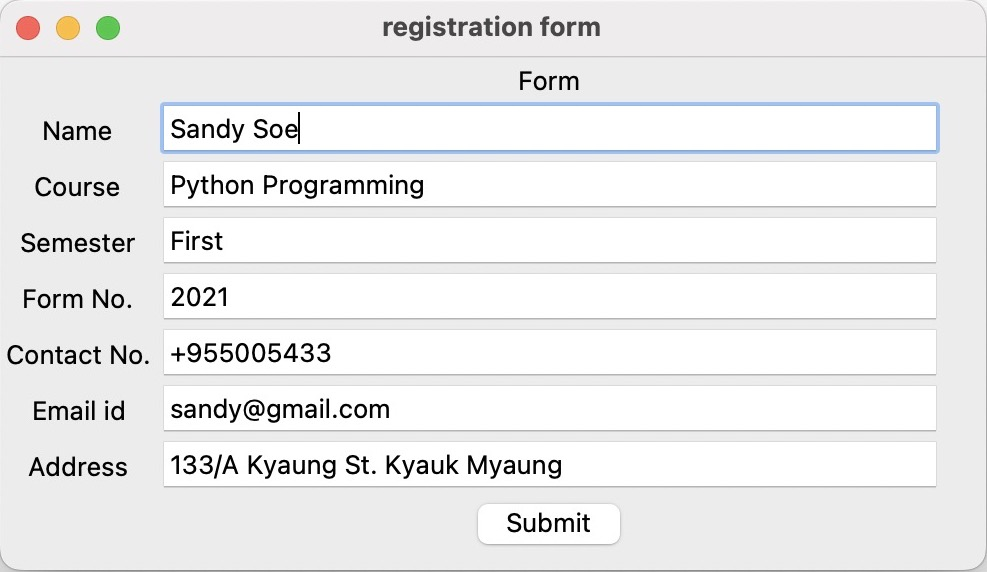
\includegraphics[width=.75\textwidth, trim={0mm 0mm 0mm 0mm},clip]{images/ch12/stuform.jpg}};
  \drawshadow{image}
\end{tikzpicture}
\caption{} 
\label{fig:stuform}
\end{figure}
%

ဒီလို အပ်ပလီကေးရှင်းမျိုးတွေကို ဒေတာဘေ့စ် အပ်ပလီကေးရှင်းလို့ ခေါ်ပါတယ်။ အချက်အလက်တွေ \fEn{create, read, update, and delete} လုပ်တဲ့ အခြေခံလုပ်ဆောင်ချက် လေးခု ပါဝင်တာကြောင့်မို့ \fEn{CRUD} အပ်ပလီကေးရှင်းလို့လည်း ခေါ်ကြတယ်။  

\subsection*{Psycopg ဒေတာဘေ့စ် ဒရိုက်ဗာ}
% Psycopg is the most popular PostgreSQL database adapter for the Python programming language. 
\fEn{Python} နဲ့ \fEn{PostgreSQL} ချိတ်ဆက်လုပ်ဆောင်ဖို့အတွက် \fEn{Psycopg} (ဆိုက်ကော့ပ်ဂျီ) ဟာ လူကြိုက်အများဆုံး ဒေတာဘေ့စ် ဒရိုက်ဗာ ဖြစ်ပါတယ်။ ဒေတာဘေ့စ် ဒရိုက်ဗာဆိုတာ ဒေတာဘေ့စ်နဲ့ \fEn{programming language} ကြား ပေါင်းကူးတံတားအဖြစ် ဆောင်ရွက်ပေးတဲ့ လိုက်ဘရီပါ။ ဒေတာဘေ့စ် အဒပ်တာ \fEn{(adapter)} လို့လည်းခေါ်တယ်။

\fEn{DBMS} နဲ့ \fEn{programming language} အလိုက် သက်ဆိုင်ရာ ဒေတာဘေ့စ် ဒရိုက်ဗာကို ရွေးချယ် အသုံးပြုရမှာပါ။ \fEn{PostgreSQL} အတွက် \fEn{Python} မှာ \fEn{Psycopg 2} နဲ့ \fEn{Psycopg 3} ရှိမယ်။ အခြားဟာတွေလည်း ရှိပါသေးတယ်။ \fEn{MySQL} အတွက် \fEn{MySQL Connector/Python} သုံးကြတယ်။ \fEn{Microsoft SQL} အတွက်ဆိုရင် \fEn{pyodbc} ဒရိုက်ဗာ။ 

\fEn{Psycopg 3} က ဗားရှင်းပိုမြင့်ပေမဲ့ ဒီစာအုပ်မှာ \fEn{Psycopg 2} ကိုပဲ အသုံးပြုပါမယ်။ \fEn{Psycopg 2} သုံးတတ်ရင် \fEn{Psycopg 3} ပြောင်းသုံးလည်း အခက်အခဲ သိပ်မရှိနိုင်ဘူး။ ဘီဂင်နာအတွက် စလေ့လာရတာ ပိုအဆင်ပြေမယ် ယူဆတာကြောင့် \fEn{Psycopg 2} သုံးဖို့ ဆုံးဖြတ်ရတာပါ။ နောက်ပိုင်း အတွေ့အကြုံရှိလာရင် ဗားရှင်းအမြင့်ကို ဆက်လေ့လာလို့ရပါတယ်။ \fEn{Psycopg 2} ကို အောက်ပါအတိုင်း \fCode{pip} ကွန်မန်းနဲ့  အင်စတောလ်လုပ်ပါ။
%
\begin{codetxt}
pip install psycopg2-binary 
\end{codetxt}
%


\subsection*{Connecting to PostgreSQL}
ဒေတာဘေ့စ် အပ်ပလီကေးရှင်းတွေဟာ \fEn{client-server} အပ်ပလီကေးရှင်းတွေလို့ ရှေ့ပိုင်းမှာ ပြောခဲ့တာ မှတ်မိမယ်ထင်ပါတယ်။ အချက်အလက်တွေ အပြန်အလှန် ပေးပို့လုပ်ဆောင်နိုင်ဖို့ \fEn{client} နဲ့ \fEn{server} ကြား ကွန်နက်ရှင် ချိတ်ဆက်ဖို့လိုတယ်။ ဒီလိုချိတ်ဆက်တဲ့အခါ \fEn{TCP/IP (Transmission Control Protocol/Internet Protocol)} ကို အသုံးပြုရပါတယ်။ \fEn{CRUD} အော်ပရေးရှင်း တစ်ခုခု လုပ်မယ်ဆို ပထမဆုံး ကွန်နက်ရှင်အရင် ရှိထားရမှာပါ။ ကွန်နက်ရှင်မရရင် ဒေတာဘေ့စ်နဲ့ ပါတ်သက်တဲ့ အခြားကိစ္စတွေ ဆက်လုပ်လို့ မရနိုင်ဘူး။ 

ပထမ ဥပမာအနေနဲ့ \fEn{Python} ပရိုဂရမ်ကနေ \fEn{PostgreSQL} ဒေတာဘေ့စ် အသစ်တစ်ခု ဘယ်လိုဆောက်ရမလဲ ကြည့်ရအောင်။ 
%
\begin{py}
# File: db_connect.py
import psycopg2

# Connect to the default PostgreSQL database to create 
# the new "students" database
conn = psycopg2.connect(
    dbname="postgres",
    user="postgres",
    password="asdfgh",
    host="localhost",
    port="5432"
)

conn.autocommit = True
cur = conn.cursor()

# Create the "students" database
cur.execute("DROP DATABASE IF EXISTS students")
cur.execute("CREATE DATABASE students")

# Close the initial connection
cur.close()
conn.close()
\end{py}
%

ဒီပရိုဂရမ်ကို တစ်ခုချင်း ခွဲခြမ်းစိတ်ဖြာ ကြည့်ပါမယ်။ \fCode{psycopg2} လိုက်ဘရီ ပထမဆုံး အင်ပို့ လုပ်ထားတယ်။ ပြီးတော့ \fCode{connect} ဖန်ရှင်နဲ့ ကွန်နက်ရှင်ယူတယ်။ \fCode{connect} ဖန်ရှင် ပါရာမီတာတွေက \fEn{psql} နဲ့ ကွန်နက်လုပ်တဲ့အခါ ထည့်ပေးရတာတွေနဲ့ တူတူပါပဲ။
%
\begin{itemize}
    \item \fCode{dbname} (ချိတ်ဆက်မဲ့ ဒေတာဘေ့စ်နံမည်) 
    \item \fCode{user} (ဒေတာဘေ့စ် ချိတ်ဆက်အသုံးပြုမဲ့ \fEn{user}) 
    \item \fCode{password} (ဒေတာဘေ့စ်ကို ချိတ်ဆက်အသုံးပြုမဲ့ \fEn{user} ရဲ့ \fEn{password})
    \item \fCode{host} (ချိတ်ဆက်မဲ့ ဆာဗာရဲ့ \fEn{Host Name/IP Address})
    \item \fCode{port} (\fEn{PostgreSQL port} နံပါတ်)
\end{itemize}
%

\fEn{Connect} လုပ်တာ အောင်မြင်ရင် \fCode{connect} ဖန်ရှင်က \fCode{connection} အော့ဘ်ဂျက်တစ်ခု ပြန်ရပါတယ်။ တကယ်လို့ ပြဿနာ တစ်ခုခုကြောင့် \fEn{connect} လုပ်လို့ မရရင်တော့ ဖြစ်ရတဲ့ အကြောင်းအရင်းပေါ် မူတည်ပြီး \fCode{OperationalError}\fEn{,} \fCode{InternalError} စတဲ့ \fEn{exception} တွေ တက်နိုင်တယ်။ ဒီ \fEn{exception} တွေက \fCode{psycopg2.Error}  ရဲ့ \fEn{subclass} တွေပါ။


%
\begin{py}
conn.autocommit = True
\end{py}
%
ဒါက ဒေတာဘေ့စ် \fEn{auto-commit mode} ကို \fEn{on} လုပ်ပေးဖို့။ ဒေတာဘေ့စ် \fEn{transaction} နဲ့ ဆိုင်တဲ့ \fEn{setting} တစ်ခုဖြစ်ပြီး နောက်ပိုင်းမှာ အသေးစိတ် ရှင်းပြမှာပါ။ \fEn{Psycopg} က သူ့နဂိုအတိုင်းဆိုရင်  \fEn{auto-commit mode} ကို \fEn{off} လုပ်ထားတယ်။ ဒေတာဘေ့စ် အသစ်ဆောက်တဲ့ \fCode{CREATE DATABASE} လို တချို့ \fEn{SQL} စတိတ်မန့်တွေက \fEn{auto commit} ကို \fEn{on} လုပ်ပေးရတယ်လို့ လောလောဆယ် သိထားရင် လုံလောက်ပါပြီ။ \fEn{Auto-commit on} ထားရင် \fEn{SQL} စတိတ်မန့်တွေ \fCode{execute} လုပ်ပြီးရင် \fCode{commit} ဖန်ရှင် ခေါ်ဖို့ မလိုဘူး။ (နောက် ဥပမာမှာ \fCode{commit} ဖန်ရှင် သုံးထားတာ တွေ့ရမှာပါ)။

\fEn{SQL} စတိတ်မန့်တွေ ဒေတာဘေ့စ်ဆီ ပေးပို့လုပ်ဆောင်စေခြင်း၊ ဒေတာဘေ့စ်ဆီက ပြန်ရလာတဲ့ ရလဒ်တွေကို အသုံးပြုခြင်း၊ ဒေတာဘေ့စ် \fEn{transaction} စီမံခြင်း စတဲ့ ကိစ္စတွေအတွက် \fEn{cursor} က အဓိကကျတယ်။ \fEn{Cursor} အော့ဘ်ဂျက်ကို \fEn{connection} ကနေ တစ်ဆင့် အခုလို ယူရပါတယ်
%
\begin{py}
cur = conn.cursor()
\end{py}
%

ချိတ်ဆက်ထားတဲ့ ဒေတာဘေ့စ်ဆီကို \fEn{SQL} စတိတ်မန့်တွေ ပေးပို့ လုပ်ဆောင်ခိုင်းဖို့ \fCode{execute} ဖန်ရှင် အသုံးပြုတယ်။  
%
\begin{py}
cur.execute("DROP DATABASE IF EXISTS students")
cur.execute("CREATE DATABASE students")
\end{py}
%
 ပထမ တစ်ကြောင်းက \fCode{students} ဒေတာဘေ့စ် ရှိပြီးသားဆိုရင် ဖျက်ပစ်မှာပါ။ ပြီးတော့မှ ဒုတိယ တစ်ကြောင်းမှာ ဒေတာဘေ့စ် အသစ်ဆောက်ပါတယ်။ ရှိပြီးသားဆိုရင် ဖျက်ပြီး အသစ်ပြန်ဆောက်တဲ့ သဘောပါ။ \fEn{psql} နဲ့ဆိုရင် \fEn{SQL} စတိတ်မန့်အဆုံးမှာ \fCode{;} ထည့်ပြီး \fEn{run} ရမှာ ဖြစ်ပေမဲ့ \fEn{Psycopg} မှာတော့ ထည့်စရာ မလိုဘူး။ ထည့်ပေးလည်း ပြဿနာတော့ မရှိဘူး။


\fEn{Cursor} နဲ့ \fEn{connection} ကို အသုံးပြုပြီးသွားရင် ပိတ်ပေးရပါမယ်။ \fEn{Exception handle} လုပ်မယ်ဆိုရင် \fCode{finally} ထဲမှာ ပိတ်သင့်တယ်။ ဒီဥပမာမှာတော့ ဒီတိုင်းပဲ ပိတ်ထားပါတယ်။
%
\begin{py}
cur.close()
conn.close()
\end{py}
%
ဒီပရိုဂရမ် \fEn{run} ပြီး \fEn{error} လည်း မတက်ဘူးဆိုရင် \fEn{students} ဒေတာဘေ့စ် ဆောက်ပြီးသွားမှာပါ။ \fEn{psql} ကနေ \mintinline{text}|\l| ကွန်မန်းနဲ့ စစ်ကြည့်နိုင်ပါတယ်။









ဒေတာဘေ့စ်ထဲမှာ \fEn{table} တွေ ဆောက်ပါမယ်။ လက်ရှိအသုံးပြုမဲ့ ဒေတာဘေ့စ်နဲ့ \fEn{connection} အရင်ယူရမယ်။ \fEn{students} ဒေတာဘေ့စ်မှာ  \fEn{table} ဆောက်မှာ။ ဒီတော့ ချိတ်ဆက်မဲ့ \fCode{dbname} က \fCode{students} ဖြစ်တယ်။ ကျန်တာတွေက ရှေ့ကနဲ့ တူတူပဲ။
%
\begin{py}
# File: db_create_student_tbl.py
import psycopg2

# Now, connect to the "students" database to create the "student" table
conn = psycopg2.connect(
    dbname="students",
    user="postgres",
    password="asdfgh",
    host="localhost",
    port="5432"
)
conn.autocommit = False
cur = conn.cursor()

# Create the "student" table
cur.execute("""
    CREATE TABLE student (
        id SERIAL PRIMARY KEY,
        name VARCHAR(100),
        age INT,
        grade VARCHAR(2)
    )
""")

# Commit changes and close the connection
conn.commit()
cur.close()
conn.close()
\end{py}
%
ကွန်နက်ရှင် ရပြီး နောက်မှာ
%
\begin{py}
conn.autocommit = False
\end{py}
%
နဲ့ \fEn{auto-commit mode} ကို \fEn{off} လုပ်တယ်။ \fEn{Psycopg} \fEn{default} က \fEn{auto-commit off} ဖြစ်တဲ့အတွက် ဒါမပါရင်လည်း \fEn{off} ဖြစ်နေမှာပါ။ ဒါဆို ဘာလို့ တကူးတက ထည့်ထားလည်းဆိုတော့ ကုဒ်ကို ဖတ်တဲ့အခါ \fEn{auto-commit off} ထားတယ်ဆိုတာ သိသာစေချင်တာရော ဒရိုက်ဗာရဲ့ \fEn{default} က \fEn{on/off} ဘာလဲ မသေချာမှာ စိုးလို့ပါ။  

\fCode{CREATE TABLE} စတိတ်မန့်က  \fEn{auto-commit mode} \fEn{on} ဖြစ်ဖြစ်၊ \fEn{off} ဖြစ်ဖြစ် \fEn{run} လို့ရတယ်။ အခု \fEn{off} လုပ်ထားတာက ရှေကဥပမာမှာ \fEn{on} လုပ်ထားတာနဲ့ ကွာခြားချက်တချို့ကို သိအောင်လို့ပါ။ အခြားထူးခြားတဲ့ အကြောင်းအရင်း မရှိပါဘူး။ နောက်ပိုင်း \fEn{database transaction} အပိုင်းမှာ \fEn{off} လုပ်ကို လုပ်ရတဲ့ အကြောင်းအရင်းကို ရှင်းပြပါမယ်။


\fEn{Auto-commit} \fEn{off} ထားရင် \fEn{SQL} စတိတ်မန့် \fEn{execute} လုပ်ပြီး \fEn{commit} လုပ်ပေးဖို့ လိုတယ်။ ဒီအတွက်
%
\begin{py}
conn.commit()
\end{py}
%
လုပ်ရပါမယ်။ \fCode{commit} မလုပ်မိရင် \fEn{execute} လုပ်ထားတဲ့ \fEn{SQL} က သက်ရောက်မှု ရှိမှာမဟုတ်ပါဘူး။ ဆိုလိုတာက \fEn{student table} ဆောက်တဲ့ကိစ္စက အတည်ဖြစ်မသွားဘူး (\fEn{rollback} ဖြစ်သွားတယ်လို့ ခေါ်တယ်)။ \fEn{Commit} နဲ့ \fEn{rollback} အကြောင်း \fEn{transaction} အပိုင်းမှာ ရှင်းပြပါမယ်။

အကယ်၍ \fEn{Auto-commit} \fEn{on} ထားရင်တော့ ကိုယ်တိုင် \fCode{conn.commit()} လုပ်မပေးရဘူး၊ ဒေတာဘေ့စ်က \fEn{SQL} ကွန်မန်း တစ်ခု \fEn{execute} လုပ်ပြီးတိုင်း အလိုအလျောက် \fEn{commit} လုပ်ပေးမှာပါ။ \fEn{Off} ထားရင် \fEn{commit} လုပ်ပေးရမယ်၊ \fEn{on} ဆိုရင် မလုပ်ပေးရဘူးလို့ မှတ်နိုင်ပါတယ်။


\section{Parameterized SQL}
\fEn{SQL} စတိတ်မန့်တွေမှာ ပါရာမီတာ ထည့်လို့ရအောင် ဒေတာဘေ့စ် ဒရိုက်ဗာတွေက ထောက်ပံပေးထားပါတယ်။ ပါရာမီတာပါတဲ့ \fEn{SQL} ကို \fEnEmp{Parameterized SQL} လို့ခေါ်တယ်။ ပုံမှန် ရိုးရိုး \fEn{SQL} နဲ့ \fEn{parameterized SQL} အသုံးပြုပုံ နှစ်ခုယှဉ်ကြည့်ပါ
%
\begin{py}
# normal SQL, no parameter
cur.execute("SELECT * FROM student WHERE age = 19 AND grade = 'A'")
\end{py}
%
%
\begin{py}
# File: db_parameterized_sql.py
# parameterized SQL
age = int(input("Age: "))
grade = input("Grade: ")
cur.execute("SELECT * FROM student WHERE age = %s AND grade = %s",
            (age, grade))
\end{py}
%
\mintinline{text}|%s| က ပါရာမီတာ၊ ပါရာမီတာတွေနေရာ ရှိရမဲ့ တန်ဖိုးအသီးသီးကို \fEn{tuple} နဲ့ ထည့်ပေးရပါမယ်။ \fCode{execute} လုပ်တဲ့အခါ ပါရာမီတာတစ်ခုစီကို သက်ဆိုင်ရာတန်ဖိုး အစားထိုးပေးမှာပါ။ \fEn{Tuple} ဟာ \fEn{list} နဲ့ဆင်တူတဲ့ စထရက်ချာ တစ်မျိုးပါပဲ။ ကွာခြားချက် တချို့ကတော့ \fEn{list} ကို \fCode{[]} သုံးတယ်၊ \fEn{tuple} အတွက် \fCode{()} သုံးတယ်။ \fEn{Tuple} က \fEn{immutable} ဖြစ်ပြီး \fEn{item} တစ်ခုပဲဆိုရင် ကော်မာထည့်ပေးရပါမယ်။ $val_1$ တစ်ခုပဲဆို \mintinline[escapeinside=ßß]{text}|(ß$val_1$ß,)| လို့ ရေးရမှာပါ။ \fEn{Parameterized SQL} မှာ ပါရာမီတာ တစ်ခုတည်းဆိုရင် ဒီအချက်ကို သတိပြုဖို့ လိုပါတယ်။ အောက်မှာ \fCode{(stu\_id,)} ဖြစ်ရပါမယ်။ ကော်မာ မထည့်ဘဲ \fCode{(stu\_id)} လို့ ရေးမိရင် အယ်ရာတက်မှာပါ။
%
\begin{py}
stu_id = int(input("ID: "))
cur.execute("SELECT * FROM student WHERE id = %s", (stu_id,))
\end{py}
%

\fEn{Parameterized SQL} နဲ့ \fEn{insert} ဘယ်လိုလုပ်ထားလဲ အောက်မှာ လေ့လာကြည့်ပါ။ \fCode{students} \fEn{list} ထဲမှာ ကျောင်းသားတစ်ယောက်ချင်းအတွက် \fEn{tuple} တွေ ထည့်ထားပြီး \fCode{for} \fEn{loop} နဲ့ တစ်ခုချင်း \fEn{insert} လုပ်သွားတာကို ဂရုစိုက် နားလည်အောင် ကြည့်ပါ။
%
\begin{py}
# File: db_insert1.py
import psycopg2

conn = psycopg2.connect(dbname="students", user="postgres",
                        password="asdfgh", host="localhost", port="5432")
conn.autocommit = False
cur = conn.cursor()

# Insert records into the student table one at a time
students = [
    ('Amy', 20, 'A'),
    ('Sandy', 22, 'B'),
    ('Kathy', 21, 'C')
]

for student in students:
    cur.execute("""
        INSERT INTO student (name, age, grade)
        VALUES (%s, %s, %s)
    """, student)

conn.commit()
cur.close()
conn.close()
\end{py}
%


ရှေ့က ဥပမာဟာ အောက်ပါ \fEn{insert} စတိတ်မန့် သုံးခုကို တစ်ခုပြီးတစ်ခု ဒေတာဘေ့စ်ဆီ ပေးပို့ လုပ်ဆောင်စေမှာပါ။ 

%
\begin{sql}
INSERT INTO student (name, age, grade) VALUES ('Amy', 20, 'A');
INSERT INTO student (name, age, grade) VALUES ('Sandy', 22, 'B');
INSERT INTO student (name, age, grade) VALUES ('Kathy', 21, 'C');
\end{sql}
%

\fEn{Insert} သုံးခုလုံး တစ်ခါတည်းနဲ့ ပေးပို့ လုပ်ဆောင်စေချင်ရင် \fCode{executemany} ကို သုံးပါတယ်။ \fEn{Tuple array} တစ်ခု ထည့်ပေးရပါမယ်။ \fEn{Array} ထဲက \fEn{tuple} တစ်ခုချင်းအတွက် \fEn{SQL} စတိတ်မန့် တစ်ခုစီ ထုတ်ပေးပြီး အသုတ်လိုက် ဒေတာဘေ့စ်ဆီ ပို့ပေးပါတယ်။
%
\begin{py}
# File: db_insert2.py
students = [
    ('Amy', 20, 'A'),
    ('Sandy', 22, 'B'),
    ('Kathy', 21, 'C')
]

cur.executemany("""
    INSERT INTO student (name, age, grade)
    VALUES (%s, %s, %s)
""", students)
\end{py}
%
စောစောကဥပမာနဲ့ ရလဒ်အားဖြင့်တော့ တူတူပါပဲ။ တစ်ကြောင်းချင်း ပို့တာနဲ့  သုံးကြောင်းလုံး အသုတ်လိုက် တစ်ခါတည်း ပို့တာပဲ ကွာပါတယ်။ အသုတ်လိုက် ပို့တာက နက်ဝပ်အသွားအပြန် \fEn{(network round-trip)} လုပ်ရတာ မများတဲ့အတွက် \fEn{record} တွေ အများကြီး \fEn{insert} လုပ်တဲ့အခါ သိသိသာသာ ပိုပြီးတော့မြန်မှာပါ။ တစ်ကြောင်းချင်း ပို့တာက တစ်ခါပို့တိုင်း နက်ဝပ်အသွားအပြန် ရှိတဲ့အတွက် ပိုကြာမယ်။ နှစ်မျိုးလုံး သူ့နေရာနဲ့သူ ချင့်ချိန်အသုံးပြုရမှာပါ။ ဒါနဲ့ပါတ်သက်လို့ အခုဆက်လက် ဆွေးနွေးမှာ မဟုတ်ပေမဲ့ ဘယ်လိုအခြေအနေမျိုးမှာ ဘယ်ဟာသုံးသင့်လဲ ဆုံးဖြတ်တတ်အောင် ဆက်လက်လေ့လာဖို့ လိုပါလိမ့်မယ်။ 

\section{\fSecCodeBf{fetch}-ing and Using Results}
\fEn{Select} စတိတ်မန့်ရဲ့ ရလဒ် \fEn{record} တွေကို \fCode{fetchall}\fEn{,} \fCode{fetchmany}\fEn{,} \fCode{fetchone} ဖန်ရှင်တွေနဲ့ ရယူအသုံးပြုနိုင်ပါတယ်။ 

\fCode{fetchall} က \fEn{record} အကုန်လုံးကို တစ်ခါတည်းနဲ့ ရယူပေးမှာပါ။ \fEn{Select} လုပ်တဲ့ \fEn{record} အရေအတွက် များလွန်းရင် ဒေတာဘေ့စ်ကနေ \fEn{Python} ပရိုဂရမ်ဘက်ကို ဒေတာအားလုံး လွှဲပြောင်းရောက်ရှိချိန် ကြာနိုင်တဲ့အပြင် ရောက်ရှိလာတဲ့ \fEn{record} တွေအတွက် ကွန်ပျူတာ မမ်မိုရီသုံးရတာကလည်း ပမာဏ များနိုင်ပါတယ်။ \fCode{fetchall} သုံးမယ်ဆိုရင် \fEn{record} အရေအတွက်ကို ထည့်စဉ်းစားဖို့ လိုပါမယ်။
%
\begin{py}
# File: db_select_and_fetch.py
cur.execute("SELECT * FROM student")

rows = cur.fetchall()
for row in rows:
    print(row)
\end{py}
%

\fCode{fetchone} ကိုတော့ \fEn{record} တစ်ခုပဲ ပြန်ရမှာ သေချာတဲ့ အခြေအနေမျိုးမှာ သုံးပါတယ်။ ဥပမာ \fEn{primary key} နဲ့ \fEn{select} လုပ်တဲ့အခါ \fEn{record} တစ်ခုထက် ပိုမရနိုင်ဘူး။
%
\begin{py}
# File: db_select_and_fetch.py
cur.execute("SELECT * FROM student WHERE id = 1")
row = cur.fetchone()
print(row)
\end{py}
% 

\fCode{fetchmany} ကတော့ လိုသလောက် \fEn{record} အရေအတွက်ကိုပဲ ရယူဖို့အတွက်ပါ။ \fEn{Record} အခု ၁၀၀ ရှိတာကို တစ်ခေါက်ကို ၂၀ နဲ့ ၅ ခါ ခွဲပြချင်တဲ့ အခါမျိုးမှာ သုံးနိုင်ပါတယ်။ 
%
\begin{py}
rows = cur.fetchmany(20)
\end{py}
%

\subsection*{Pagination}
\fEn{Record} တွေ အများကြီး တစ်ခါတည်းနဲ့ ပြမဲ့အစား နည်းနည်းချင်း ခွဲပြီး ပြပေးတဲ့နည်းကို အပ်ပလီကေးရှင်းတွေမှာ အသုံးများတာ တွေ့ရပါတယ်။ \fEn{Pagination} လို့ ခေါ်ပါတယ်။ \fEn{Page} တစ်ခုမှာ သတ်မှတ်ထားတဲ့ \fEn{record} အရေအတွက်ကို ပြပေးပြီး \fEn{user} က နောက် \fEn{page} တစ်ခုချင်း ဆက်ကြည့်လို့ရအောင် စီစဉ်ပေးထားတာပါ။ အောက်ပါ ဥပမာမှာ \fCode{fetchmany} သုံးထားတာ လေ့လာကြည့်ပါ။

%
\begin{py}
# File: db_pagination1.py
# Function to fetch a page of student records using fetchmany
def fetch_page(page_size):
    # Fetch rows in batches using fetchmany
    rows = cur.fetchmany(page_size)
    return rows

cur.execute("SELECT * FROM student ORDER BY id")

page_size = 2    # Number of records per page
page_number = 1  # Start with page 1

while True:
    students = fetch_page(page_size)
    
    if not students:
        break  # No more records, exit loop
    
    print(f"Page {page_number}:", students)
    page_number += 1
\end{py}
%

\fCode{fetchmany} နဲ့ နည်းလမ်းအပြင် \fEn{SQL language} ရဲ့ \fCode{LIMIT} နဲ့ \fCode{OFFSET} အသုံးပြုပြီး \fEn{pagination} လုပ်နိုင်ပါတယ်။ 
%
\begin{py}
# File: db_pagination2.py
# Function to fetch a page of student records
def fetch_page(page_size, page_number):
    offset = (page_number - 1) * page_size

    # SQL query with LIMIT and OFFSET for pagination
    select_query = """
        SELECT * FROM student
        ORDER BY id
        LIMIT %s OFFSET %s
    """

    cur.execute(select_query, (page_size, offset))
    rows = cur.fetchall()

    return rows
\end{py}
% 
\fCode{OFFSET} နဲ့ \fCode{LIMIT} ဟာ “\fEn{page} နံပါတ်” နဲ့ “တစ် \fEn{page} မှာ ပါရှိရမဲ့ \fEn{record} အရေအတွက်” ကို ကိုယ်စားပြုတာလို့ အကြမ်းဖျဉ်း ပြောလို့ရပါတယ်။ ဒီနည်းက \fEn{record} အရမ်းများပြီး \fEn{page} အရေအတွက်များတယ်၊ \fEn{page} တစ်ခုချင်း အစဉ်အတိုင်းမဟုတ်ဘဲ ဟိုကျော်ဒီကျော် ကြည့်လို့ရအောင် လုပ်ဖို့လိုတဲ့ အခြေအနေမျိုးမှာ ပိုပြီးအဆင်ပြေနိုင်ပါတယ်။ ပရိုဂရမ်ကုဒ် အပြည့်အစုံကို သက်ဆိုင်ရာ ဖိုင်မှာ ကြည့်နိုင်ပါတယ်။

\subsection*{\fSubSecCodeBf{rowcount} Attribute}
\fEn{Insert, update, delete} လုပ်တာဆိုရင်တော့ \fEn{insert, update, delete} လုပ်လိုက်တဲ့ \fEn{record} အရေအတွက်ကို \fCode{rowcount} \fEn{attribute} နဲ့ သိနိုင်ပါတယ်။
%
\begin{py}
# File: db_update_and_rowcount.py
cur.execute("""
    UPDATE student
    SET grade = %s
    WHERE name = %s
""", ('A+', 'Amy'))
print(cur.rowcount)
\end{py}
%

\section{Python နဲ့ SQL အကြား ဒေတာတိုက်ပ် ပြောင်းလဲခြင်း}
ဒေတာဖော်ပြပုံ မတူကွဲပြားချက်တွေကြောင့် \fEn{Python} နဲ့ \fEn{SQL} \fEn{language} နှစ်ခုကြား ဒေတာအမျိုးအစား လိုက်လျောညီထွေဖြစ်အောင် ပြောင်းလဲမှုတွေ အပြန်အလှန် လုပ်ဆောင်ဖို့ လိုအပ်ပါတယ်။ \fEn{SQL} ပါရာမီတာနေရာမှာ \fEn{Python} ဒေတာတန်ဖိုး အစားထိုးတဲ့အခါ ဒေတာတိုက်ပ် ပြောင်းလဲခြင်းကို \fEn{Psycopg} က လုပ်ဆောင်ပေးပါတယ်။ %ဒေတာဘေ့စ်ကနေ ပြန်ရလာတဲ့ ရလဒ်တွေကို သင့်တော်တဲ့ \fEn{Python} ဒေတာတိုက်ပ်အဖြစ် ပြောင်းလဲပေးခြင်း တို့ကို \fEn{Psycopg} က လုပ်ဆောင်ပေးပါတယ်။ 
%
\begin{py}
# File: db_datatype_conv.py
# select account transactions between two dates
cur.execute("""
    SELECT * FROM account_transaction 
        WHERE txn_date BETWEEN %s AND %s
""", (datetime(2024, 8, 1), datetime(2024, 8, 31)))
rows = cur.fetchall()
\end{py}
% 
\fEn{Python} \fCode{datetime} ကို သင့်တော်တဲ့ \fEn{SQL} ဒေတာအဖြစ် ပြောင်းလဲပေးဖို့ လိုမယ်ဆိုတာ မြင်နိုင်ပါတယ်။ ဒေတာဘေ့စ်ဆီ ပေးပို့မဲ့ \fEn{SQL} ကို အခုလို \fCode{mogrify} ဖန်ရှင်နဲ့ ထုတ်ကြည့်လို့ ရတယ်
%
\begin{py}
sql_str = cur.mogrify("""
    SELECT * FROM account_transaction 
        WHERE txn_date BETWEEN %s AND %s
""", (datetime(2024, 8, 1), datetime(2024, 8, 31)))
print(sql_str.decode('utf-8'))
\end{py}
%
ဒီလို ပြောင်းပေးထားတာ တွေ့ရမှာပါ 
%
\begin{codetxt}
SELECT * FROM account_transaction 
    WHERE txn_date BETWEEN '2024-08-01T00:00:00'::timestamp 
        AND '2024-08-31T00:00:00'::timestamp
\end{codetxt}
%
ဒီတိုင်း စမ်းကြည့်ပါ  
%
\begin{py}
print(cur.mogrify("SELECT %s, %s, %s;", (None, True, False))
         .decode('utf-8'))
# ß\fEn{Output:}ß 'SELECT NULL, true, false;'
print(cur.mogrify("SELECT %s, %s, %s, %s;",
                  (10, 25 ** 25, 10.0, Decimal("10.00"))).decode('utf-8'))
# ß\fEn{Output:}ß 'SELECT 10, 88817841970012523233890533447265625, 10.0, 10.00;'
\end{py}
%
\fCode{None} ကို \fCode{NULL} ပြောင်းပေးပါတယ်။ \fCode{bool}\fEn{,} \fCode{int}\fEn{,} \fCode{long}\fEn{,} \fCode{Decimal} စတာတွေကိုလည်း သင့်တော်တဲ့ \fEn{SQL} တိုက်ပ်အဖြစ် ပြောင်းပေးတယ်။ 

\fEn{Select} လုပ်တဲ့ ရလဒ်ဒေတာတွေကိုလည်း သင့်တော်တဲ့ \fEn{Python} ဒေတာတိုက်ပ် ပြောင်းပေးမှာပါ။ \fEn{Select} လုပ်ရင် \fEn{row} တွေကို \fEn{list} တစ်ခုအနေနဲ့ ရတယ်။ အဲဒီ \fEn{list} ထဲမှာ \fEn{row} တစ်ခုကို \fEn{tuple} တစ်ခုနဲ့ ဖော်ပြတယ်။ \fEn{Row} ကို \fEn{tuple} အနေနဲ့ ဖော်ပြတဲ့အခါ \fEn{column} တန်ဖိုး တစ်ခုချင်းကို \fEn{SQL} ဒေတာ\\တိုက်ပ် အပေါ်မူတည်ပြီး သက်ဆိုင်ရာ \fEn{Python} ဒေတာတိုက်ပ် ပြောင်းပေးပါတယ်။ \fEn{Python} နဲ့ \fEn{SQL} ဒေတာတိုက်ပ် တစ်ခုချင်းအတွက် လိုက်လျောညီထွေဖြစ်အောင် အပြန်အလှန်တွဲဖက်ပေးထားပုံကို \fEn{Psycopg documentation} စာမျက်နှာမှာ အသေးစိတ် ဖော်ပြထားပါတယ် 

\begin{vbtm}
https://www.psycopg.org/docs/usage.html#python-types-adaptation
\end{vbtm}

\section{Dynamic SQL}
ပရိုဂရမ်ကုဒ်ထဲမှာ ပုံသေရေးထားတာ မဟုတ်ဘဲ ပရိုဂရမ် \fEn{run} တဲ့ အချိန်ကျမှ လိုသလို တည်ဆောက်ယူတဲ့ \fEn{SQL} ကို \fEn{Dynamic SQL} လို့ ခေါ်ပါတယ်။ \fEn{Table} နံမည် ထည့်ပေးလိုက်၊ အဲ့ဒီ \fEn{table} ထဲက \fEn{record} တွေကို ထုတ်ပြရမယ်ဆိုပါစို့။ \fEn{Select} စတိတ်မန့်မှာ \fEn{table} နံမည်က ပုံသေဖြစ်လို့ မရတော့ဘူး။ ပထမဆုံး စဉ်းစားမိတာက \fEn{SQL} ကို \fEn{string} နှစ်ခုဆက်ပြီး ထုတ်မယ်ပေါ့။
%
\begin{py}
# Never do like this!!!
tbl_name = input("Enter table name: ")
select_tbl_sql = "SELECT * FROM " + tbl_name 
\end{py}
%
ဒါဟာ လူပြိန်းနည်းနဲ့ \fEn{dynamic SQL} ထုတ်တဲ့ အရိုးရှင်းဆုံး ဥပမာတစ်ခုပဲ။ ဒီနည်းနဲ့ ရတယ်ဆိုပေမဲ့ ရှားရှားပါးပါး ကြုံရခဲတဲ့ ချွင်းချက်အခြေအနေ တချို့ကလွဲလို့ \fEn{string} ဆက်ပြီး \fEn{SQL} ထုတ်တာက လုံးဝကို မလုပ်သင့်တဲ့ အရာပါ။ ဒါတင် မဟုတ်သေးဘူး။ \fEn{f-strings}\fEn{,} \fCode{str.format()}\fEn{,} \fEn{template string}\fEn{,} ပုံစံဟောင်း \mintinline{text}|%| အော်ပရိတ်တာ စတာတွေကိုလည်း \fEn{dynamic SQL} ထုတ်ဖို့ မသုံးသင့်ဘူး။ (\fEn{Python} မှာ \fEnEmp{string interpolation} ပုံစံအမျိုးမျိုးရှိတယ်၊ \fEn{f-strings} ကို စာမျက်နှာ \fRefNo{\pageref{ch07:f-string}} အခန်း \fRefNo{\ref{ch:ch07ctlstmt}} မှာ ဖော်ပြခဲ့ဖူးတယ်၊ \fEn{Python string interpolation} အကြောင်း \fCode{https://tinyurl.com/y4jju285} မှာ ပြည့်ပြည့်စုံစုံ ရှင်းပြထားတာ တွေ့နိုင်တယ်)။ ဘာကြောင့် မသုံးသင့်တာလဲ အကြောင်းအရင်းကို ဒီအခန်း နောက်ဆုံးပိုင်းမှာ အားနည်းချက်/ပြဿနာတွေကို ဖော်ပြထားတာ ဖတ်ပြီးရင် နားလည်သွားပါလိမ့်မယ်။ 


\fEn{Dynamic SQL} အတွက် \fEn{Psycopg} မှာ \fEn{sql} မော်ဒျူး ရှိပါတယ်။ \fEn{String interpolation} နဲ့ \fEn{SQL} ထုတ်ရင် ဖြစ်နိုင်တဲ့ ပြဿနာတွေကို ဖြေရှင်းပေးထားတယ်။ \fEn{Table} နံမည် \fEn{dynamic SQL} ကို အခုလို ရေးရမယ်။
%\fEn{SQL string} ထဲမှာ \fEn{table, column} စတဲ့ \fEn{identifier} တွေကို ပါရာမီတာအနေနဲ့ ထားမယ်ဆိုရင် \mintinline{text}|{}| ကို သုံးရပါမယ်။ \fEn{Select} စတိတ်မန့်မှာ \fEn{table} နံမည် ပုံသေမထားဘဲ ပြောင်းလို့ရချင်တယ် ဆိုပါစို့။ အခုလို လုပ်ရမှာပါ
%
\begin{py}
# File: db_dynamic_sql1.py   
# reqire sql module
from psycopg2 import sql

tbl_name = input("Enter table name: ")
query = sql.SQL("SELECT * FROM {}").format(sql.Identifier(tbl_name))
cur.execute(query)
\end{py}
%
\fEn{SQL string} အစိတ်အပိုင်းတစ်ခုကို ကိုယ်စားပြုဖော်ပြဖို့အတွက် \fCode{sql.SQL} အော့ဘ်ဂျက် သုံးရပါတယ်။ ၎င်းအော့ဘ်ဂျက် ကိုယ်စားပြုတဲ့ \fEn{SQL} အစိတ်အပိုင်းထဲမှာ \mintinline{text}|{}| ကို ဖြည့်ပေးရမဲ့ နေရာအဖြစ် ယာယီ သတ်မှတ်ပေးနိုင်တယ်။ အဲဒီနေရာကို ဖြည့်ပေးဖို့ \fCode{format} မက်သဒ်ကို သုံးရပါမယ်။ အပေါ်က \fCode{SELECT} \fEn{SQL} မှာ \mintinline{text}|{}| ကို \fEn{table} နေရာမှာ ပထမ ထည့်ထားတယ်။ ပြီးတော့မှ \fCode{format} မက်သဒ်ခေါ်ပြီး အဲ့ဒီနေရာမှာ \fCode{tbl\_name} ဖြည့်တယ်။ \mintinline{text}|{}| နေရာမှာ \fEn{string} တိုက်ရိုက် အစားမထိုးဘဲ \fCode{sql.Identifier} အော့ဘ်ဂျက် ပြောင်းပေးဖို့တော့ လိုတယ်။

% ဒီအော့ဘ်ဂျက် ကိုယ်စားပြုတာက စတိတ်မန့် တစ်ကြောင်းလုံး အပြည့်အစုံ ဖြစ်နိုင်သလို \fCode{FROM}\fEn{,} \fCode{WHERE}\fEn{,} \fCode{ORDER BY} စတဲ့ \fEn{SQL} အစိတ်အပိုင်း တစ်ခုခုလည်း ဖြစ်လို့လည်းရတယ်။ 
% အဲဒီနေရာမှာ \fCode{format} မက်သဒ်နဲ့ \fEn{table/column} ရဲ့ နံမည်ကို အစားထိုး ဖြည့်ပေးနိုင်တယ်။ \fEn{Table/column} နံမည်ကို \fCode{sql.Identifier} အော့ဘ်ဂျက် ပြောင်းပြီးမှ အစားရပါမယ်။ \fEn{String} အတိုင်း ထည့်လို့တော့ မရဘူး။

%၊ \fCode{format} က \mintinline{text}|{}| နေရာမှာ \fEn{identifier} (\fEn{table} နံမည်၊ \fEn{column} နံမည် စတာတွေကို ဆိုလိုတာ) တစ်ခုခု အစားထိုးဖို့။ \fCode{format} လုပ်တဲ့အခါ \fEn{string} ကို \mintinline{text}|sql.Identifier| အော့ဘ်ဂျက်အနေနဲ့ ထည့်ပေးရပါမယ်။ 

\mintinline{text}|{}| နဲ့ \mintinline{text}|%s| နှစ်ခုလုံးကို ဖြည့်ပေးရမဲ့ နေရာတွေအတွက် သုံးတယ် ဆိုပေမဲ့ \mintinline{text}|{}| က \fEn{table} နံမည်၊ \fEn{column} နံမည် စတဲ့ \fEn{identifier} တွေအတွက်၊ \mintinline{text}|%s| ကိုက ဒေတာတန်ဖိုးတွေအတွက် သုံးတာ၊ ရည်ရွယ်ချက်ချင်းမတူပါဘူး။ အောက်ပါ ဥပမာကို ကြည့်ပါ။
%
\begin{py}
# File: db_dynamic_sql2.py 
table = 'student'
col1 = 'grade'
col2 = 'age'
query = sql.SQL("SELECT * FROM {} WHERE {} = %s AND {} = %s").format(
    sql.Identifier(table), sql.Identifier(col1), sql.Identifier(col2))
# see the formatted result
print(query.as_string(conn))
cur.execute(query, ('A+', 20))
\end{py}
%
\fCode{format} မက်သဒ်နဲ့ \fEn{table} နဲ့ \fEn{column} နှစ်ခုနေရာကို \fCode{table}\fEn{,} \fCode{col1}\fEn{,} \fCode{col2} အစားထိုးပေးပါတယ်။ \fCode{WHERE} အပိုင်းမှာ \fEn{column} တစ်ခုချင်းအတွက် တန်ဖိုးကို \mintinline{text}|%s| ထည့်ထားတယ်။ \fCode{query} ကို \fCode{execute} လုပ်တဲ့အခါမှ \mintinline{text}|%| နေရာမှာ \fEn{tuple} \fCode{('A', 20)} ထဲက တန်ဖိုးနဲ့ အစားထိုးမှာပါ။

\fEn{Dynamic SQL} အတွက် \fCode{sql.SQL} အော့ဘ်ဂျက်မှာ \fCode{join} မက်သဒ်ကလည်း အသုံးဝင်တယ်။ နံမည်က \fCode{join} ဆိုတဲ့အတိုင်း \fEn{column} နံမည်တွေ ကော်မာနဲ့ဆက်တာ၊ ကွန်ဒီရှင်တွေ \fCode{AND}\fEn{/}\fCode{OR} နဲ့ ဆက်တာ စတဲ့ကိစ္စတွေအတွက် ကူညီပေးတဲ့ မက်သဒ်ဖြစ်ပါတယ်။ အသုံးပြုပုံ လေ့လာကြည့်ပါ။
%
\begin{py}
col_names = ['id', 'name', 'age', 'grade']
col_identifiers = []
for col in col_names:
    col_identifiers.append(sql.Identifier(col))
sql_frag1 = sql.SQL(", ").join(col_identifiers)
print(sql_frag1.as_string(conn)) # ß\fEn{Output:} ß "id", "name", "age", "grade"
\end{py}
%

%
\begin{py}
# File: db_dynamic_sql2.py

# generating a full sql statement with  WHERE conditions
conditions = []
for col in col_names:
    conditions.append(sql.SQL("{} = %s").format(sql.Identifier(col)))
sql_frag2 = sql.SQL(" AND ").join(conditions)
print(sql_frag2.as_string(conn))

# generate a full sql statement
sql_full = (sql.SQL("SELECT ")
            + sql.SQL(", ").join(col_identifiers)
            + sql.SQL(" FROM student WHERE ")
            + sql.SQL(" AND ").join(conditions))
print(sql_full.as_string(conn))
cur.execute(sql_full, (1, 'Amy', 20, 'A+'))
print(cur.fetchone())
\end{py}
%
\fCode{sql.SQL} အော့ဘ်ဂျက်တွေကို \fCode{+} အော်ပရိတ်တာနဲ့  ဆက်ထားတာကိုလည်း သတိထားမိမှာပါ။

\fEn{Psycopg} ဒရိုက်ဗာ သုံးရင် အခုဖော်ပြခဲ့တဲ့ နည်းတွေနဲ့ပဲ \fEn{dynamic SQL} ထုတ်ရမယ်ကတော့ ဟုတ်ပါပြီ။ ဘာကြောင့် ဒီလောက် အလုပ်ရှုပ်ခံပြီး \fEn{dynamic SQL} ထုတ်နေရတာလဲ၊ တစ်ခါတည်း ကုဒ်ထဲမှာ \fEn{SQL string} ကိုပဲ အပြည့်အစုံရေးထားလို့ မရဘူးလား စသည်ဖြင့် မေးခွန်းထုတ်စရာ ရှိပါတယ်။ တကယ့်လက်တွေ့ အပ်ပလီကေးရှင်းတွေမှာ လိုအပ်ချက်အများစုဟာ \fEn{dynamic SQL} သုံးရတာပါ။ ပုံသေရေးထားလို့ရတဲ့ \fEn{static SQL} သုံးရတာ နည်းတယ်။ 

\subsection*{Multi-field Search}
ကျောင်းသား \fEn{record} တွေ \fEn{search} လုပ်တဲ့ ပရိုဂရမ် အစိတ်အပိုင်းတစ်ခုကို စိတ်ကူးကြည့်ပါ။ တစ်ခါ\allowbreak တစ်ရံ ကျောင်းသားနံမည်နဲ့ ရှာတယ်။ တစ်ခါတစ်ရံမှာတော့ \fEn{grade} နဲ့ ရှာချင်ရှာမယ် (ဥပမာ ဘယ်သူတွေ \fEn{grade A} ရကြလဲ)။ ဒါမှမဟုတ် နံမည်နဲ့ \fEn{grade} နှစ်ခုလုံးနဲ့ ရှာတာလည်း ဖြစ်နိုင်တာပဲ။ \fEn{Dynamic SQL} မသုံးပဲ အခုလို စမ်းကြည့်နိုင်တယ်။
%
\begin{py}
# File: multi_field_search1.py

print("Key in the value for each attribute."
      "Or press enter to ignore the attribute.")
name = input("Name: ")
grade = input("Grade: ")

sql0 = "SELECT * FROM student"
sql1 = "SELECT * FROM student WHERE name = %s"
sql2 = "SELECT * FROM student WHERE grade = %s"
sql3 = "SELECT * FROM student WHERE name = %s AND grade = %s"

if name.strip() and grade.strip():
    cur.execute(sql3, (name, grade.strip()))
elif name.strip():
    print(name.strip())
    cur.execute(sql1, (name.strip(),))
elif grade.strip():
    cur.execute(sql2, (grade.strip(),))
else:
    cur.execute(sql0)
\end{py}
%
နံမည်နဲ့ \fEn{grade} နှစ်ခုဆိုရင်တောင် \fCode{if} စတိတ်မန့်က အတော်လေး ရှုပ်နေပါပြီ။ \fEn{SQL} စတိတ်မန့် လေးခုကိုလည်း ကြိုတင်သတ်မှတ်ထားရသေးတယ်။ \fEn{Age} နဲ့ ရှာလို့ရအောင် ထပ်ဖြည့်မယ် ဆိုပါစို့။ အောက်ပါအတိုင်း ဖြစ်နိုင်ခြေ ၈ ခု တွဲလို့ရမှာပါ။
\begin{align*}
&(name, age, grade),\\
&(name, age), (name, grade), (grade, age),\\
&(name), (age), (grade),\\
&()    
\end{align*}
သုံးခုနဲ့တင် အတော်လေး ရှုပ်နေပါပြီ။ ပါရာမီတာတွေသာ ထပ်တိုးလာတာနဲ့အမျှ \fEn{SQL} တွေ၊ ဖြစ်နိုင်တဲ့ အတွဲတွေနဲ့ စစ်ရမဲ့ ကွန်ဒီရှင်တွေကလည်း ဖေါင်းပွလာမှာ။ ဒီလိုအခြေအနေမျိုးမှာ \fEn{Dynamic SQL} က အများကြီး အဆင်ပြေစေတယ်။ အောက်မှာ ရေးထားတဲ့ ပရိုဂရမ်ကုဒ်ကို လေ့လာကြည့်ပါ။
%
\begin{py}
# File: multi_field_search2.py
# This program illustrates searching students by multiple columns

name = input("Name: ")
grade = input("Grade: ")
age = input("Age: ")

search_params = {
    'name': name.strip() if name.strip() else None,
    'age': int(age.strip()) if age.strip() else None,
    'grade': grade.strip() if grade.strip() else None
}

query = sql.SQL("SELECT * FROM student")

# List to hold the WHERE conditions
conditions = []
# List to hold the values
values = []

# Build conditions dynamically based on user input
for column, value in search_params.items():
    if value is not None:
        conditions.append(sql.SQL("{} = %s").format(sql.Identifier(column)))
        values.append(value)

# If there are any conditions, add them to the query
if conditions:
    query = query + sql.SQL(" WHERE ") + sql.SQL(" AND ").join(conditions)
\end{py}
%
နောက်ထပ် ပါရာမီတာတစ်ခု ထပ်ထည့်လည်း နည်းနည်းပဲ ပြင်ဖို့လိုတယ်။ ကျောင်းသား \fEn{id} နဲ့လည်း ရှာလို့ရချင်ရင် \fEn{input} ဖတ်တာနဲ့ ပါရာမီတာတွေ ထည့်တဲ့ \fEn{map} မှာ ထပ်ထည့်ရုံပဲ။
%
\begin{py}
# ß\fEnEmp{others inputs}ß
id = input("ID: ")

search_params = {
    # ß\fEnEmp{others params}ß
    'id': int(id.strip()) if id.strip() else None
}
\end{py}
%

အခုတွေ့ခဲ့တာက \fEn{search} ကို နမူနာအနေနဲ့ ပြထားတာပါ။ \fEn{CRUD} လုပ်တဲ့အခါ \fEn{dynamic SQL} ဟာ \fEn{insert, select, update, delete} လေးခုလုံးအတွက် သုံးရပါတယ်။ (\fEn{Psycopg} မဟုတ်တဲ့) အခြား ဒေတာဘေ့စ် လိုက်ဘရီတွေမှာလည်း \fEn{dynamic SQL} အတွက် သူ့နည်းသူ့ဟန်နဲ့ ထောက်ပံ့ပေးထားတာ တွေ့ရမှာဖြစ်ပြီး လိုက်ဘရီ မတူတဲ့အတွက် အသုံးပြုပုံလည်း ကွာခြားမယ်ဆိုပေမဲ့  အခုဖော်ပြခဲ့တဲ့ အခြေခံ သဘောတရားတွေ နားလည်ရင် သိပ်အခက်အခဲမရှိဘဲ ဆက်လက်လေ့လာလို့ရမှာပါ။

\section{Database Transactions}
အောက်ဖော်ပြပါ လုပ်ငန်းကိစ္စတွေကို စဉ်းစားကြည့်ပါ။
%
\begin{itemize}
    \item ဘဏ်အကောင့် ငွေလွှဲခြင်း
    \item ဟိုတယ် \fEn{booking}
    \item \fEn{Online} မှ ပစ္စည်းဝယ်ယူခြင်း
\end{itemize}
%
ဒီလို လုပ်ငန်းကိစ္စတစ်ခု ပြီးမြောက်ဖို့အတွက် ဆောင်ရွက်ပေးရတဲ့ လုပ်ငန်းစဉ်မှာ အဆင့်ဆင့် ပါဝင်တယ်။ ဘဏ်အကောင့် တစ်ခုနဲ့ တစ်ခု ငွေလွှဲတဲ့အခါ လွှဲသူ အကောင့်ကနေ ငွေကြေးပမာဏတစ်ခု နှုတ်ရမှာဖြစ်ပြီး လက်ခံအကောင့်ထဲကို ပေါင်းပေးရပါမယ်။ ဟိုတယ် \fEn{booking}  လုပ်ရင်လည်း ကတ်စတမ်မာ တည်းမဲ့ရက် အခန်းရနိုင်/မရနိုင် စစ်ကြည့်ပြီး အခန်း ဖယ်ထားပေးရပါမယ်။ အခန်းခ စရံငွေအတွက် ကတ်စတမ်မာ အကောင့်ကနေ ပိုက်ဆံပေးချေရမယ်။ နောက်ဆုံးမှာ \fEn{booking} လုပ်ထားပြီးကြောင်း ကွန်ဖန်းလုပ်ဖို့ အီးမေးလ်ပို့ပေးရပါမယ်။ ထိုနည်းတူစွာ \fEn{online} ကနေ ပစ္စည်းဝယ်တာကို ခွဲခြမ်းစိတ်ဖြာ ကြည့်ရင်လည်း အဆင့် တစ်ခုမက ပါဝင်နေတာ တွေ့ရမှာပါ။

ဖော်ပြပါ ဥပမာတစ်ခုစီကို ကြည့်ရင် လုပ်ငန်းစဉ်တစ်ခုလုံး  ပြီးမြောက်ဖို့အတွက် ၎င်းလုပ်ငန်းစဉ်မှာ ပါဝင်တဲ့အဆင့်အားလုံး ပြဿနာ တစ်စုံ\allowbreak တစ်ရာ မရှိဘဲ အောင်မြင်ပြီးစီးအောင် ဆောင်ရွက်ရမှာပါ။ ငွေလွှဲတဲ့အခါ ကိုယ့်ဆီကပဲ ပိုက်ဆံဖြတ်သွားပြီး တစ်ဖက်လူဆီ မရောက်မှာ စိုးရိမ်မိတာ ကျွန်တော်တို့အားလုံး ဖြစ်ဖူးမှာပါ။ ဟိုတယ် \fEn{booking} လုပ်တဲ့ ကိစ္စမှာဆိုရင် အခန်းကို ကတ်စတမ်မာအတွက် ချန်ထားပြီးခါမှ အကြောင်းတစ်ခုခုကြောင့် စရံငွေဖြတ်လို့မရရင် ဟိုတယ်အနေနဲ့ ပြဿနာရှိပါတယ်။ အဲဒီ့အခန်းကို အခြားသူအတွက်လည်း ငှါးလို့မရ ဖြစ်နေမှာပါ။ 

\begin{figure}[thb!]%
\subfloat[]{\hspace{-10.5pt} \incfig[0.98]{txncommit}}\hfill%
\vspace{1\baselineskip}
\subfloat[]{\hspace{-10.5pt} \incfig[0.98]{txnrollback}}%
\caption{Database transaction သဘောတရား။ Dashed စတုဂံအကြီးဟာ transaction စကုပ်၊ ထောင့်လုံး စတုဂံအသေးတွေက အကောင့်နှစ်ခုရဲ့ လက်ကျန်ငွေ အချိန်နဲ့အမျှ ပြောင်းလဲနေပုံ၊ မြှားဟာ အချိန် စီးဆင်းရာ။   (က) Transaction ကို commit လုပ်တဲ့အခါ ၎င်း transaction စကုပ် အတွင်း update လုပ်ထားတာတွေက အတည်ဖြစ်သွားပါတယ်။ (ခ) Rollback လုပ်ရင်တော့ transaction စကုပ်ထဲရှိ update တွေ ပျက်ပြယ်သွားပြီး လက်ကျန်ငွေ မပြောင်းလဲဘဲ နဂိုအတိုင်း ရှိနေမှာပါ}
\label{fig:txn_commit_rollback}
\end{figure}

အခုလို ပြဿနာမျိုးတွေ မဖြစ်အောင် ကာကွယ်ဖို့ ဒေတာဘေ့စ်တွေမှာ \fEnEmp{transaction} သဘောတရားကို ထည့်သွင်းတည်ဆောက် ပေးထားပါတယ်။ \fEn{Transaction} ဆိုတာ လုပ်ငန်းကိစ္စတစ်ခုအနေနဲ့ တစ်ပေါင်းတစ်စည်းတည်း ရှုမြင်တဲ့ ‘လုပ်ငန်းစဉ် အဆင့်ဆင့်’ လို့ ယူဆနိုင်တယ်။ အဲ့ဒီ လုပ်ငန်းစဉ် အဆင့်ဆင့်ဟာ ဒေတာဘေ့စ် \fEn{read/write/update} အော်ပရေးရှင်းတွေ ပါဝင်နိုင်တယ်။ \fEn{Transaction} အတွင်း လုပ်ငန်းစဉ် အဆင့်အားလုံး အောင်မြင်ပြီးစီးသွားတာ၊ ဒါမှမဟုတ် ဘယ်တစ်ခုကိုမှ မလုပ်ဆောင်ဖြစ်တာ နှစ်မျိုးပဲ ဖြစ်နိုင်ပါတယ်။ တချို့ပဲ လုပ်ဖြစ်သွားပြီး အကြောင်း တစ်ခုခုကြောင့် တချို့ကို မလုပ်ဖြစ်ဘဲ ကျန်ခဲ့တယ်ဆိုတာမျိုး လုံးဝမဖြစ်နိုင်ဘူး (ဥပမာ \fEn{transaction} အတွင်းမှာ ငွေလွှဲတဲ့ ကိစ္စလုပ်ရင် အကောင့်တစ်ခုကနေပဲ ပိုက်ဆံဖြတ်သွားပြီး တစ်ဖက်အကောင့်မှာ မဝင်သွားတာ မဖြစ်နိုင်တော့ဘူး)။ \fEn{Transaction} တစ်ခု အတွင်းက အချက်အလက် အပြောင်းအလဲ မှန်သမျှဟာ ၎င်း \fEn{transaction} ကို \fEn{commit} မလုပ်မချင်း အတည်မဖြစ်သေး၊ ယာယီသာဖြစ်တယ်။ ၎င်းတို့ကို အတည်ဖြစ်စေချင်ရင် \fEn{commit} လုပ်ရပါမယ်၊ အကယ်၍ ပယ်ဖျက်ပြီး အားလုံးနဂိုအတိုင်း ပြန်ရှိစေချင်ရင် \fEn{rollback} လုပ်နိုင်ပါတယ်။ ပုံ (\fRefNo{\ref{fig:txn_commit_rollback}}) မှာ \fEn{commit} နဲ့ \fEn{rollback} အလုပ်လုပ်ပုံ သဘောတရားကို တွေ့ရပါမယ်။ အချက်အလက် မှန်ကန်စိတ်ချရခြင်း \fEn{(data integrity)} အတွက် အာမခံချက် အပြည့်အဝ ပေးနိုင်ပြီး တစ်ဝက်တစ်ပျက် လုပ်ဆောင်မှုတွေကြောင့် ဒေတာဘေ့စ် မှန်ကန်ကိုက်ညီမှု မရှိခြင်း အခြေအနေကို ကာကွယ်ဖို့ရာအတွက် \fEn{transaction} သဘောတရားဟာ အလွန်အရေးပါတယ်။ 





\fEn{Transaction} နဲ့ ပါတ်သက်ပြီး နောက်ထပ်အရေးပါတဲ့ အချက်တစ်ခုက \fEn{isolation} သဘောတရားပါ။ \fEn{Transaction} တစ်ခုအတွင်း လုပ်ဆောင်ထားတဲ့ ဒေတာအပြောင်းအလဲတွေဟာ (\fEn{update, insert, delete} ကို ဆိုလိုတာ) အဲဒီ \fEn{transaction} မပြီးမချင်း ဘယ်သူကမှ မမြင်ရဘူး။ တစ်နည်းအားဖြင့် \fEn{transaction} တစ်ခု \fEn{commit} မလုပ်ရသေးခင်မှာ ၎င်းအတွင်းရှိ ကြားကာလ အခြေအနေကို အခြား \fEn{transaction} တွေကနေ တွေ့မြင်ရမှာ မဟုတ်ပါဘူး (\fEn{Isolation level} ပေါ်မှာတော့ မူတည်တယ်)။ \fEn{Isolation} ဟာ ဒေတာမှန်ကန်ကိုက်ညီခြင်း အတွက် အရေးကြီးပါတယ်။ \fEn{Transaction} မပြီးစီးခင် ကြားကာလဟာ မှန်ကန်ကိုက်ညီခြင်း မရှိသေးတဲ့ အခြေအနေမှာ ရှိနေနိုင်ပါတယ် (ပုံ \fRefNo{\ref{fig:txn_commit_rollback}} ရဲ့ $t_3$ နဲ့ $t_4$ ကြားကာလကို စဉ်းစားကြည့်ပါ)။ အဲဒီလို အနေအထားကို ပြင်ပကနေ မမြင်နိုင်အောင် \fEn{isolation} နဲ့ ကာကွယ်ပေးထားတာပါ။ 

\begin{mytcboxflt}
%ဒေတာဘေ့စ်တွေမှာ \fEn{isolation} ဘယ်လောက်ထိ တင်းကြပ်ဖို့ လိုလဲ ဆိုတာပေါ်မူတည်ပြီး ရွေးချယ်နိုင်တဲ့ \fEn{isolation level} လေးမျိုး အနိမ့်ကနေ အမြင့် အခုလို အစဉ်အတိုင်း 
ဒေတာဘေ့စ်တွေမှာ \fEn{isolation level} (၄) မျိုး ရှိပါတယ်။ \fEn{Isolation} အလျော့အတင်း အလိုက် \fEn{level} အခုလို စဉ်ထားပါတယ်
%
\vspace{0.5\baselineskip}
\begin{itemize}
    \setlength\itemsep{0.25em}
    \item \fEn{Read Uncommitted}
    \item \fEn{Read Committed (default)}
    \item \fEn{Repeatable Read}
    \item \fEn{Serializable}
\end{itemize}
\vspace{0.5\baselineskip}
%
ဒေတာဘေ့စ် အများစုမှာ \fEn{Read Committed} က \fEn{default} ပါ။ \fEn{Transaction} တစ်ခု \fEn{commit} မလုပ်ရသေးတာတွေကို အခြားကနေ မြင်ရနိုင်တဲ့ \fEn{Read Uncommitted} ကိုတော့ အသုံးပြုတာ မတွေ့ရသလောက်ပါပဲ။ \fEn{Isolation level} မြင့်လေ  \fEn{concurrency} အားနည်းလေလို့ ယေဘုယျ ပြောနိုင်ပါတယ်။   
\end{mytcboxflt}

\fEn{Transaction} အကြောင်း အတန်အသင့်နားလည်ပြီး \fEn{SQL} နဲ့ \fEn{Psycopg} မှာ ဘယ်လို ဖန်တီးအသုံးပြုရလဲ ကြည့်ရအောင်။ \fCode{BEGIN}\fEn{,} \fCode{COMMIT}\fEn{,} \fCode{ROLLBACK} တို့ဟာ \fEn{transaction} နဲ့ဆိုင်တဲ့ \fEn{SQL} ကွန်မန်းတွေ။ \fCode{BEGIN} က \fEn{transaction} အစပြုပေးတဲ့ ကွန်မန်းဖြစ်တယ်။ \fCode{COMMIT} လုပ်ရင် \fEn{transaction} တစ်ခုလုံးကို (ပါဝင်တဲ့ အဆင့်အားလုံးကိုဆိုလို) အတည်ပြုပေးမှာဖြစ်ပြီး \fCode{ROLLBACK} လုပ်ရင် \fEn{transaction} တစ်ခုလုံးကို ပြန်လည်ရုတ်သိမ်းပေးမှာပါ။ \fCode{COMMIT} (သို့) \fCode{ROLLBACK} လုပ်တဲ့အခါ \fEn{transaction} လည်း ပြီးဆုံးပါတယ်။ နောက်ထပ် အသစ်တစ်ခုလိုအပ်ရင် \fCode{BEGIN} နဲ့ ပြန်စရပါမယ်။  

\fEn{psql} မှာ စမ်းကြည့်မယ်ဆိုရင် \fCode{AUTOCOMMIT} ကို \fEn{off} ပေးရပါမယ် (\fEn{default} က \fEn{on} ထားတယ်)။ \mintinline{text}|\set| ကွန်မန်းနဲ့ အခုလို \fEn{run} ထားပါ။
%
\begin{codetxt}
\set AUTOCOMMIT off
\end{codetxt}
%
အခုလို ပြန်စစ်ကြည့်ပါ။ \fEn{Off} ဖြစ်နေသင့်ပါတယ် (ပုံ \fRefNo{\ref{fig:tx}} မှာ ကြည့်ပါ)။
\begin{codetxt}
\echo :AUTOCOMMIT
\end{codetxt}

ဆက်လက်ပြီး အောက်ပါအတိုင်း စမ်းကြည့်ပါ။ \fCode{BEGIN} ကွန်မန်းနဲ့ \fEn{transaction} ကို စတင်ပါတယ်။ \fEn{Transaction} ထဲမှာ \fCode{UPDATE} နှစ်ခု \fEn{run} ပြီး \fCode{COMMIT} လုပ်တယ်။ \fCode{UPDATE} နှစ်ခုလုံး \fEn{run} ပြီးတော့မှ \fCode{COMMIT} မလုပ်ဘဲ \fCode{ROLLBACK} လုပ်ရင် အကောင့်နှစ်ခုလုံး \fEn{transaction} မစခင် မူလအနေအထားအတိုင်း ရှိနေမှာပါ။ 

\fEn{Isolation} နဲ့ \mintinline{text}|COMMIT/ROLLBACK| အလုပ်လုပ်ပုံ သဘောတရားကို \fEn{psql} နောက်ထပ်တစ်ခု ဖွင့်ပြီး စစ်ဆေး စမ်းသပ် ကြည့်နိုင်ပါတယ်။ ပထမ \fEn{psql} မှာ \fEn{SQL} တစ်ခု \fEn{run} ပြီးတိုင်း နောက် \fEn{psql} တစ်ခုကနေ \fCode{SELECT} လုပ်ပြီး စောင့်ကြည့်လေ့လာပါ။ နမူနာ စမ်းကြည့်ထားတာကို ပုံ (\fRefNo{\ref{fig:txchk}}) မှာ တွေ့နိုင်တယ်။ ပထမ \fCode{SELECT} ရလဒ်တွေမှာ ဒေတာအပြောင်းအလဲ ဖြစ်တာ မတွေ့ရသေးပါဘူး။ နောက်ဆုံး \fCode{SELECT} က ပထမ \fEn{psql} မှာ \fCode{COMMIT} လုပ်ပြီးမှ \fEn{run} ထားတာပါ။ အဲဒီ ရလဒ်မှာ အကောင့် \fEn{record} နှစ်ခု အမှန်တကယ် \fEn{update} ဖြစ်သွားတာကို တွေ့ရမှာပါ။ 

%
\begin{sql}
/* ß\fEn{Transaction in SQL}ß */
BEGIN;
UPDATE account SET balance = balance - 50000.00 
    WHERE acc_no = '0086-6002-1111';
UPDATE account SET balance = balance + 50000.00 
    WHERE acc_no = '0086-6002-3311';
-- ß\fEnEmp{etc etc}ß
COMMIT;
\end{sql}
%

\begin{figure}[tbh!]
\begin{tikzpicture}
  \node[anchor=south west,inner sep=0] (image) at (0,0)
  {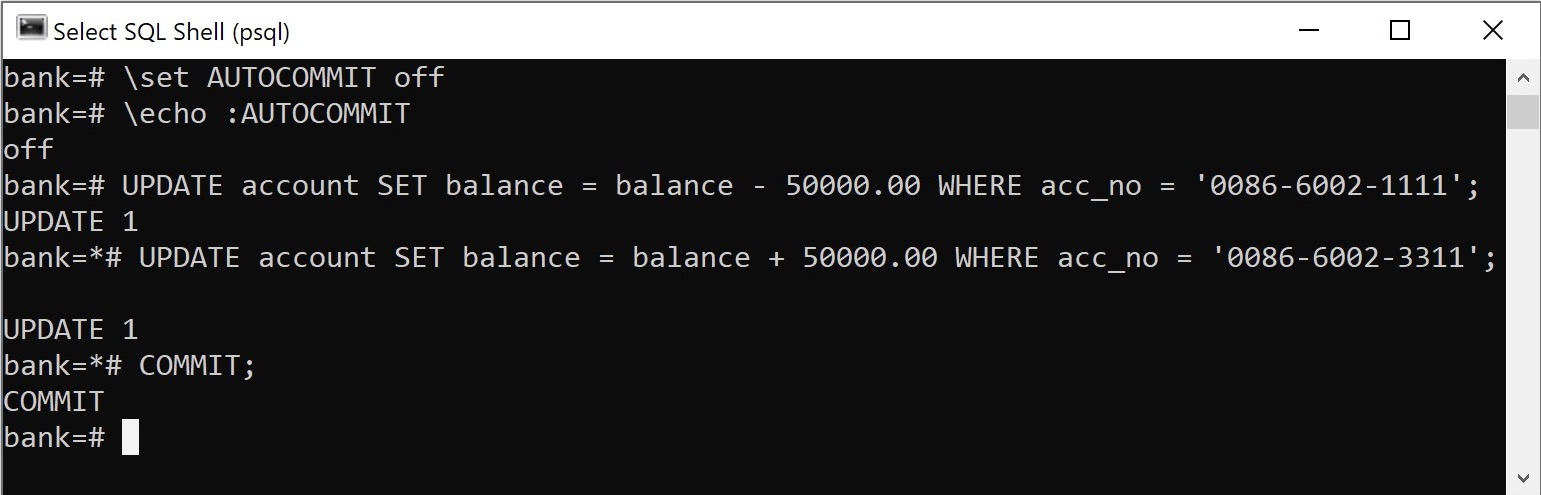
\includegraphics[width=.98\textwidth, trim={0mm 0mm 0mm 1mm},clip]{images/ch12/tx.jpg}};
  \drawshadow{image}
\end{tikzpicture}
\caption{psql မှတစ်ဆင့် transaction တစ်ခု ဖန်တီးအသုံးပြုပုံ} 
\label{fig:tx}
\end{figure}


\begin{figure}[!htb]
\begin{tikzpicture}
  \node[anchor=south west,inner sep=0] (image) at (0,0)
  {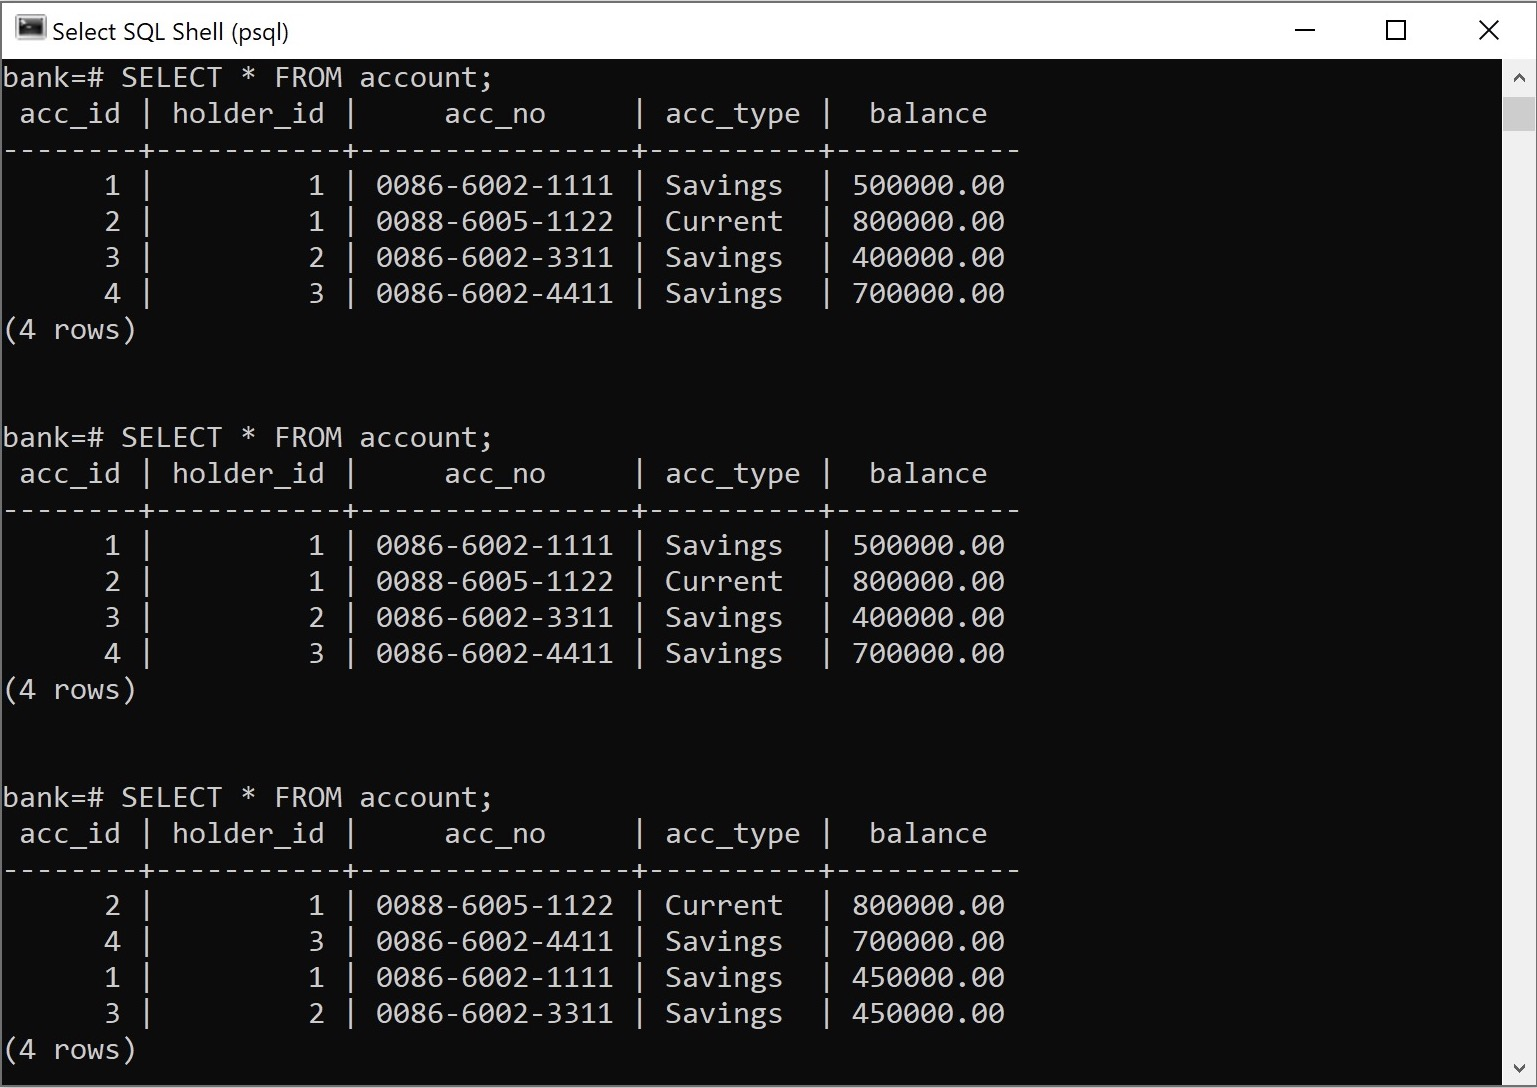
\includegraphics[width=.98\textwidth, trim={0mm 0mm 0mm 1mm},clip]{images/ch12/tx_check.jpg}};
  \drawshadow{image}
\end{tikzpicture}
\caption{အခြား transaction တစ်ခုကို psql မှ စောင့်ကြည့်ပုံ}
\label{fig:txchk}
\end{figure}

\fEn{Psycopg} ဒရိုက်ဗာက သူ့နဂိုအတိုင်းဆိုရင် \fCode{AUTOCOMMIT} ပိတ်ပြီးသားပါ။ ပထမဆုံး \fCode{execute} လုပ်တဲ့အခါ \fEn{transaction} ကို အလိုအလျောက် စပေးပါတယ် (\fCode{execute} လုပ်ပြီဆိုတာနဲ့ \fCode{BEGIN} ကို အရင်လုပ်ပေးမှာပါ)။ \fCode{COMMIT} လုပ်ရင် \fCode{conn.commit()}\fEn{,} \fCode{ROLLBACK} ဆိုရင် \fCode{conn.rollback()} ခေါ်ပေးရပါမယ်။ \fCode{commit()} မလုပ်မိဘဲ ကွန်နက်ရှင် ပိတ်လိုက်ရင် \fEn{transaction} အတွင်း လုပ်ထားသမျှ ဒေတာအပြောင်းအလဲ အားလုံး အတည်မဖြစ်တော့ဘဲ အားလုံး ပျက်ပြယ်သွားပါမယ်။ 

\fEn{Psycopg} နဲ့ \fEn{transaction} စီမံတဲ့ နမူနာပုံစံကို အောက်မှာကြည့်ပါ။ \fEn{Transaction} စီမံတဲ့နေရာမှာ \fEn{exception handling} က အရေးပါပါတယ်။ \fCode{try} ထဲမှာ \fEn{transaction} မှာ ပါဝင်တဲ့ အဆင့်တွေကို လုပ်ဆောင်ရလေ့ရှိတယ်။ အခု ဥပမာမှာ \fEn{update} နှစ်ခု လုပ်ထားတယ်။ နှစ်ခုလုံး ပြဿနာမရှိဘဲ ပြီးရင် \fCode{commit} လုပ်သွားမယ်။ အကြောင်းတစ်ခုခုကြောင့် \fEn{exception} တက်ခဲ့ရင် \fCode{except} ဘလောက်ထဲ ရောက်ပြီး \fCode{rollback} ဖြစ်မှာပါ။
%
\begin{py}
# File: db_transaction_eg1.py
# ß\fEn{Transaction in Python with Psycopg}ß
import psycopg2

conn = psycopg2.connect(dbname="bank", user="postgresql", 
                        password="asdfgh", host="localhost", port="5432")
cur = conn.cursor()

try:
    cur.execute("UPDATE account SET balance = balance - 50000.00 "
                "WHERE acc_no = '0086-6002-1111'")
    cur.execute("UPDATE account SET balance = balance + 50000.00 "
                "WHERE acc_no = '0086-6002-3311'")
    conn.commit()
except psycopg2.Error as e:
    conn.rollback()
    print("Database error: ", e)
except Exception as e:
    conn.rollback()
    print("Unknown error: ", e)
finally:
    cur.close()
    conn.close()
\end{py}
%
\fCode{except} ဘလောက်တွေမှာ \fCode{rollback} လုပ်ဖြစ်အောင် လုပ်ဖို့ သေချာဂရုစိုက်ရပါမယ်၊ မေ့ကျန်ခဲ့တာ ဖြစ်နိုင်တယ်။ ဒီလို မဖြစ်အောင် ကူညီပေးတဲ့ \fCode{with} စတိတ်မန့်ကို ပိုအသုံးများတယ်။ \fEn{Connection} နဲ့ \fEn{cursor} ကို \fCode{with} နဲ့တွဲသုံးရင် \fEn{commit, rollback} နဲ့ \fEn{cursor} ပိတ် ကိစ္စတွေကို အလိုအလျောက် လုပ်ပေးမှာမို့လို့  မေ့ကျန်ခဲ့စရာ အကြောင်း သိပ်မရှိတော့ဘူး။ \fEn{Connection} ကိုပဲ သေချာဂရုစိုက် ပိတ်ပေးဖို့ လိုတယ်။

%
\begin{py}
# File: db_transaction_eg2.py
# ß\fEn{Using}ß with ß\fEn{statement}ß

conn = None
try:
    conn = psycopg2.connect(dbname="bank", user="postgresql", 
                            password="asdfgh", host="localhost", port="5432")
    with conn:
        with conn.cursor() as cur:
            cur.execute("UPDATE account SET balance = balance - 50000.00 "
                        "WHERE acc_no = '0086-6002-1111'")
            cur.execute("UPDATE account SET balance = balance + 50000.00 "
                        "WHERE acc_no = '0086-6002-3311'")
except psycopg2.Error as e:
    print("Database error: ", e)
except Exception as e:
    print("Unknown error: ", e)
finally:
    conn.close()
\end{py}
%


\begin{mytcboxflt}
\fEn{Psycopg} ဗားရှင်း \fEn{2.5} ကစပြီး \fEn{connection, cursor} တို့ကို \fCode{with} စတိတ်မန့်နဲ့ တွဲဖက် အသုံးပြုနိုင်ပါတယ်
%
\begin{pytc}
conn = psycopg2.connect()

with conn:
    with conn.cursor() as cur:
        cur.execute(SQL1)

conn.close()
\end{pytc}
\fEn{Connection} နဲ့ဆိုင်တဲ့ \fCode{with} ဘလောက် \fEn{(outer \fCode{with})} ပြီးဆုံးသွားတယ်၊ \fEn{exception} မဖြစ်ဘူးဆိုရင် \fEn{transaction} ကို \fEn{commit}  လုပ်ပေးမှာဖြစ်ပြီး \fEn{exception} ဖြစ်ခဲ့ရင်တော့ \fEn{rollback} ဖြစ်သွားမှာပါ။ \fEn{Cursor} နဲ့ သက်ဆိုင်တဲ့ \fCode{with} ဘလောက် \fEn{(inner \fCode{with})} ပြီးဆုံးရင် \fEn{cursor} ကို အလိုအလျောက် ပိတ်ပေးမှာဖြစ်ပေမဲ့ \fEn{transaction} က ဆက်ရှိနေအုံးမှာပါ။ \fEn{Transaction commit/rollback} က \fEn{connection} နဲ့ဆိုင်တဲ့ \fCode{with} ဘလောက် အဆုံးမှာ ဖြစ်တာပါ။ \fCode{with} က \fEn{connection} ကို အလိုအလျောက် မပိတ်ပေးပါဘူး။ ဒါကြောင့် ကိုယ်တိုင် ပိတ်ပေးရပါမယ်။
\end{mytcboxflt}
\clearpage


\section{Concurrency}
ဒေတာဘေ့စ်တွေဟာ တစ်ချိန်တည်း \fEn{user} အများအပြား တစ်ပြိုင်နက် အသုံးပြုရင် ဖြစ်ပေါ်နိုင်တဲ့ \fEn{concurrency problem} တွေ မဖြစ်ပေါ်အောင် ကာကွယ်ဖို့အတွက် နည်းလမ်းတွေ ထောက်ပံပေးထားပါတယ်။ \fEnEmp{Concurrency} ဆိုတာ တစ်ခုထက်ပိုတဲ့ အလုပ်တွေ ကွန်ပျူတာက တစ်ချိန်တည်းမှာ လုပ်ဆောင်ပေးနေတာကို ဆိုလိုတာပါ။ တစ်ချိန်တည်း လုပ်ဆောင်ပေးတယ် ဆိုပေမဲ့ အားလုံး တစ်ပြိုင်နက်တည်း လုပ်ဆောင်တာ ဟုတ်ချင်မှ ဟုတ်မှာပါ။ အလုပ်တစ်ခုစီကို အလှည့်ကျ လုပ်ဆောင်ပေးပြီး တစ်ပြိုင်နက်ထဲ ဖြစ်ပျက်နေတယ်လို့ ထင်ရအောင် စီမံထားတာလည်း ဖြစ်နိုင်ပါတယ်။ 

ကလပ်စစ် \fEn{concurrency problem} ဥပမာတစ်ခုကို ဒီအပိုင်းမှာ လေ့လာကြည့်ပါမယ်။ အောက်ဖော်ပြပါ ပရိုဂရမ်ကုဒ် အစိတ်အပိုင်းဟာ ငွေထုတ်ယူတဲ့ ကိစ္စအတွက် ဖြစ်ပါတယ်။
%
\begin{py}
# Step 1: select account balance from database
cur.execute("""
    SELECT balance FROM account WHERE acc_no = %s
""", (acc_no,))
account_balance = cur.fetchone()

# Step 2: check if the balance is enough
if not account_balance:
    raise Exception("Account not found.")
elif account_balance[0] < amount:
    raise Exception("Insufficient funds in the account.")

# Step 3: Debit the account
cur.execute("""
    UPDATE account
    SET balance = balance - %s
    WHERE acc_no = %s
""", (amount, acc_no))
conn.commit()
\end{py}
%

ငွေထုတ်တဲ့ကိစ္စမှာ အကြမ်းဖျဉ်း \fEn{step} သုံးခု ပါဝင်တာ တွေ့ရမှာပါ 
%
\begin{itemize}
    \item လက်ကျန်ငွေ \fEn{select} လုပ်ခြင်း
    \item လက်ကျန်ငွေ လုံလောက်မှု ရှိ/မရှိ စစ်ဆေးခြင်း
    \item လက်ကျန်ငွေ \fEn{update} လုပ်ခြင်း
\end{itemize}
%
(ဒါ့ထက် အသေးစိတ် ထပ်ခွဲလို့ ရအုံးမှာပါ၊ ရှေ့ဆက်ရှင်းပြမဲ့ ကိစ္စအတွက် ဒီလောက်နဲ့က နားလည်ရ ပိုလွယ်ပါမယ်)။

\fEn{Concurrent} ပရိုဂရမ်တစ်ခုဟာ ငွေထုတ်သူ တစ်ဦးချင်းစီအတွက် ဒီ အစဉ်လိုက် \fEn{step} သုံးခုကို လုပ်ဆောင်ပေးရမှာပါ။ တစ်ချိန်တည်း နှစ်ယောက်ထုတ်ရင် \fEn{step} တစ်ခုစီကို တစ်ယောက် တစ်လှည့် နှစ်ယောက်လုံးအတွက် တစ်ချိန်တည်းမှာ ဆောင်ရွက်ပေးရပါမယ်။ အနီးစပ်ဆုံး မြင်သာအောင် ပြောမယ်ဆိုရင်  အဖျော်ဆရာတစ်ယောက် လက်ဖက်ရည်ဖျော်သလိုပဲ၊ တစ်ခွက်ပြီးမှ တစ်ခွက်ဖျော်တာ မဟုတ်ဘူး၊ လက်ဖက်ရည်ခွက်တွေ ရှေ့မှာစီချထားပြီး အကျရည်ထည့်၊ နို့ဆီထည့်၊ နို့စိမ်းထည့် အားလုံး တစ်ပြိုင်တည်းနီးပါး အပြီးဖျော်တာ။ အလုပ်တွေကို တစ်ချိန်တည်း လုပ်တယ်ဆိုတာ ဒီသဘောကို ဆိုလိုတာ။ 

\begin{figure}[!htb]
    \incfig[0.56]{accwithdrawconcur1}
    \caption{ငွေထုတ်ကိစ္စ နှစ်ခု တစ်ချိန်တည်း အလှည့်ကျ လုပ်ဆောင်ပုံ ဖြစ်နိုင်ခြေ ၃ ခု (အားလုံး မဟုတ်ပါ)။ concurrency သဘာဝအရ ဘယ်လို အလှည့်ကျမလဲ ဆိုတာက random ပဲ၊ ပုံသေမရှိဘူး။ ပရိုဂရမ်မာက အလှည့်ကျ အစီအစဉ်ကို လိုသလို ထိန်းကွပ်လို့ မရနိုင်ဘူး။}
    \label{fig:accwithdrawconcur1}
\end{figure}



အဖျော်ဆရာ အလုပ်လုပ်ပုံနဲ့ \fEn{concurrent} ပရိုဂရမ် လုံးဝမတူတဲ့ အချက်တစ်ခုရှိတယ်။ \fEn{Concurrency} သဘာဝအရ အလုပ်တစ်ခုစီကို အချိန်အနည်းငယ်ကြာ အလှည့်ကျ လုပ်ဆောင်ပေးပါတယ်။ ဒီလို အလှည့်ပေးစနစ်ကို \fEn{operating system} မှာ ပါဝင်တဲ့ \fEn{scheduler} က  စီမံတာဖြစ်ပြီး ပရိုဂရမ်ရေးသားသူ လိုသလို စိတ်ကြိုက် ထိန်းကွပ်လို့ မရနိုင်ပါဘူး။ ဒီအတွက်ကြောင့် အလုပ်နှစ်ခုမှာပါဝင်တဲ့ \fEn{step} တွေ ဘယ်လိုအစဉ်နဲ့ အလှည့်ကျ လုပ်ဆောင်မလဲ ပုံသေတွက်လို့မရတော့ဘူး။  



ပုံ (\fRefNo{\ref{fig:accwithdrawconcur1}}) မှာ အလုပ်နှစ်ခု အလှည့်ကျ လုပ်ဆောင်ပုံ ဖြစ်နိုင်ခြေ သုံးခုကို တွေ့ရပါမယ်။ အလုပ်နှစ်ခုကို အထက်အောက် အရောင်ခွဲ ပြထားတယ်။ စတုဂံငယ် တစ်ခုစီက ပါဝင်တဲ့ \fEn{step} တစ်ခုချင်းကို ကိုယ်စားပြုတာ၊ မြှားဟာ အချိန် စီးဆင်းရာ။ ပုံမှာပြထားတာ သုံးခုအပြင် အခြား ဖြစ်နိုင်တဲ့ အစီအစဉ်တွေ ကျန်ပါသေးတယ်။ သင်္ချာနည်းနည်းကျွမ်းတယ်၊ စိတ်ဝင်စားတယ်ဆိုရင် ဖြစ်နိုင်ခြေ အားလုံး တွက်ကြည့်လို့ရပါတယ် (\fEnEmp{Permutations with repetition} \fEn{or} \fEnEmp{combinatorics} သဘောတရားနဲ့ တွက်ရမှာပါ၊ အခုကိစ္စအတွက် ဖြစ်နိုင်ခြေ အားလုံး အခု ၂၀ ရှိပါမယ်)။




\fEn{Concurrent} အလုပ်တွေကြားမှာ အချက်အလက် မျှဝေသုံးစွဲတာ မရှိရင် ထူးထူးခြားခြား ပြဿနာ မရှိပါဘူး၊ ပရိုဂရမ် ရေးသားရတာလည်း ပုံမှန်ထက် အများကြီး မခက်ဘူး။ ဒါပေမဲ့ အချက်အလက် မျှဝေသုံးစွဲတာ ရှိခဲ့ရင်တော့ ပြဿနာရှိလာပါတယ်။ ဥပမာ အကောင့်တစ်ခုတည်းကနေ တစ်ပြိုင်တည်း ငွေထုတ်တဲ့ ဖြစ်စဉ်ကို စဉ်းစားကြည့်ပါ။ စန္ဒီနဲ့ ကေသီ နှစ်ယောက်ပေါင်း အကောင့်တစ်ခု ဖွင့်ထားတယ်။ လက်ရှိ အကောင့် လက်ကျန်ငွေ  ၅ သိန်း ရှိပြီး သူတို့ နှစ်ယောက် တစ်နေရာစီကနေ ၄ သိန်း သီးခြား ထုတ်ယူကြတာ တိုက်တိုက်ဆိုင်ဆိုင် တစ်ချိန်တည်းဖြစ်သွားတယ်လို့ စိတ်ကူးကြည့်ပါ။ ဒီဖြစ်စဉ်မှာ အကောင့် \fEn{record} ဟာ \fEn{shared data} ဖြစ်ပြီး အလုပ်နှစ်ခုက တူညီတဲ့ \fEn{record} တစ်ခုတည်းကို တစ်ချိန်တည်းမှာ \fEn{update} လုပ်ဖို့အတွက် ကြိုးစားကြတာကို တွေ့ရမှာပါ။

% (တစ်ယောက် ၄ သိန်း ထုတ်ယူမှာ)။ အကောင့်ထဲ ရှိတာမှ နှစ်ယောက်ပေါင်း ၅ သိန်းပဲ ရှိတဲ့အတွက် ၈ သိန်းထုတ်လို့ ဘယ်နည်းနဲ့မှ မရသင့်ပါဘူး။ %\fEn{Concurrent} ပရိုဂရမ် တည်ဆောက်ရတာကလည်း အများကြီး ရှုပ်ထွေးခက်ခဲလာနိုင်တယ်။ စဉ်းစားတာ တစ်ချက်လေး မှားသွားတာနဲ့  ... (\fEn{Concurrency} မှာ အားသာချက်/အားနည်းချက် အမျိုးမျိုး ရှိပါတယ်၊ အခန်း (\fRefNo{\ref{ch:concurrency}}) မှာ ဆက်လက် ဖော်ပြပေးမှာပါ)။   

%
\begin{figure}[!htb]
    \incfig[0.6]{accwithdrawconcur2}
    \caption{Concurrency problem ဥပမာ။ ၅ သိန်းရှိတဲ့ အကောင့် တစ်ခုတည်းကနေ တစ်ယောက် ၄ သိန်း၊ နှစ်ယောက် တစ်ချိန်တည်း ငွေထုတ်တဲ့အခါ step တစ်ခုချင်းအလိုက် လက်ကျန်ငွေ ပြောင်းလဲပုံ}
    \label{fig:accwithdrawconcur2}
\end{figure}
%

ပုံ (\fRefNo{\ref{fig:accwithdrawconcur1}}) အပေါ်ဆုံးကအတိုင်း အလှည့်ကျ လုပ်ဆောင်တယ် ဆိုပါစို့။ \fEn{Step} တစ်ခုချင်းအလိုက် လက်ကျန်ငွေ \fEn{balance} ပြောင်းလဲပုံကို ပုံ (\fRefNo{\ref{fig:accwithdrawconcur2}}) မှာ ပြထားတယ်။ $K_1, K_2, K_3, S_1, S_2, S_3$ တို့ဟာ ကေသီနဲ့ စန္ဒီ့အတွက် \fEn{step} သုံးခုစီလို့ ယူဆပါ \fEn{($K$ for Kathy, $S$ for Sandy)}။ $S_1, K_1, K_2, S_2$ လုပ်ဆောင်ပြီးချိန်အထိ လက်ကျန်ငွေ ၅ သိန်းဟာ နဂိုအတိုင်း မပြောင်းလဲသေးဘူး။



% အပေါ်တန်း စတုဂံ အသေးလေးတွေဟာ ကေသီငွေထုတ်တာ၊ အောက်ဖက်က စန္ဒီလို့ ယူဆပါ။ အပေါ်ဆုံး အလှည့်ကျ ပုံစံအရ $S_1, K_1, K_2, S_2, K_3, S_3$ အစဉ်နဲ့ လုပ်ဆောင်မှာပါ ($S$ နဲ့ $K$ ဟာ စန္ဒီနဲ့ ကေသီကို ကိုယ်စားပြုတာ)။  \fEn{Step} တစ်ခုချင်း ဖြစ်ပျက်တာကို လေ့လာကြည့်ရင် ပုံ (\fRefNo{\ref{fig:accwithdrawconcur2}})

$K_3$ အပြီးမှာ လက်ကျန်ငွေ \fEn{balance} ဟာ ၁ သိန်း ဖြစ်သွားပြီ။ ဒီအတိုင်းဆိုရင် နောက်\allowbreak ထပ် ၄ သိန်း ထုတ်လို့ မရသင့်တော့ဘူး။ $S_2$ မှာ လက်ကျန်ငွေ လောက်/မလောက် စစ်ခဲ့ချိန်က ဒီလိုမဟုတ်သေးဘူး၊ အဲ့တုန်းက ၅ သိန်းရှိခဲ့တာ။ ဆိုတော့ $S_2$ အရဆိုရင် $S_3$ ကို ဆက်လက်လုပ်ဆောင်ရမှာပဲ။ $S_3$ ပြီးသွားတဲ့အခါ \fEn{balance} ဟာ အနှုတ် ၃ သိန်းဖြစ်သွားပါတယ်။ ကေသီနဲ့ အေမီဟာ သူတို့မှာ ရှိတဲ့ငွေထက် ဘဏ်ကနေ ၃ သိန်း အပိုထုတ်လို့ရသွားတာ ဖြစ်ပါတယ်။  ပုံ (\fRefNo{\ref{fig:accwithdrawconcur1}}) က နောက်ထပ် ဖြစ်နိုင်ခြေ နှစ်ခုမှာလည်း ဒီပြဿနာ တွေ့ရမှာပါ။

ဘာ့ကြောင့် ဒီလို ဖြစ်ရတာလဲ၊ မဖြစ်အောင် ဘယ်လို ကာကွယ်ရမလဲ။ တစ်ချိန်တည်းမှာ ထုတ်ယူကြပေမဲ့ အကောင့်တစ်ခုတည်းကနေ မဟုတ်ရင်  ဒီလိုပြဿနာ မဖြစ်နိုင်ဘူး။ တစ်နည်းအားဖြင့် မတူညီတဲ့ သီးခြားအကောင့်တစ်ခုစီကနေ တစ်ပြိုင်နက် ငွေထုတ်ယူတာဟာ \fEn{concurrency problem} မဖြစ်စေနိုင်ဘူး။ တစ်ချိန်တည်း၊ အကောင့်တစ်ခုတည်းကနေ ငွေထုတ်တဲ့ကိစ္စနှစ်ခု တိုက်ဆိုင်တဲ့အခါ \fEn{concurrency problem} ရှိနိုင်တာပါ။ ဖြေရှင်းဖို့ နည်းလမ်းကတော့ အကောင့်တစ်ခုကို တစ်ချိန်တည်းမှာ အလုပ်တစ်ခုကပဲ \fEn{update} လုပ်လို့ရအောင် ကာကွယ်ပေးထားရပါမယ်။ \fEn{Transaction} တစ်ခုဟာ ၎င်း \fEn{update} လုပ်ဖို့ ရည်ရွယ်တဲ့ \fEn{record} ကို အခြား \fEn{transaction} တွေကနေ \fEn{update} လုပ်လို့မရအောင် \fCode{FOR UPDATE} နဲ့ တားဆီးနိုင်ပါတယ်။ \fCode{SELECT} လုပ်တဲ့အချိန်မှာ အခုလို တွဲသုံးရမှာပါ    
% အလုပ်နှစ်ခုက \fEn{row} တစ်ခုတည်းကို တစ်ချိန်တည်းမှာ \fEn{update} လုပ်တာဟာ ဒီပြဿနာရဲ့ အဓိက အကြောင်းအရင်း ဖြစ်တယ်။   
%\fEn{Select} လုပ်တဲ့ \fEn{Record locking}  ဒီလိုမဖြစ်အောင် ကာကွယ်တဲ့ နည်းလမ်းတစ်ခုက \fEn{} \fEn{update} လုပ်ဖို့ ရည်ရွယ်ချက်နဲ့ \fEn{select} အကောင့် \fEn{record} ကို \fEn{lock} လုပ်တာ။  
%
\begin{py}
# File: db_transaction_and_concurrency.py

# Step 1: select account balance from database
cur.execute("""
    SELECT balance FROM account WHERE acc_no = %s FOR UPDATE
""", (acc_no,))
account_balance = cur.fetchone()
\end{py}
% 
\fEn{Concurrency} စကားအရ ပြောရင် \fCode{FOR UPDATE} ဟာ \fEn{select} လုပ်လိုက်တဲ့ \fEn{row} တွေအပေါ်မှာ \fEn{exclusive lock} ရယူတာဖြစ်တယ်။ ဒါနဲ့ပါတ်သက်တဲ့ အသေးစိတ်ကို \fEn{concurrency} အခန်းမှာ သီးခြားရှင်းပြမှာပါ။ 

\fEn{Concurrency} ဟာ ကျယ်ပြန့်ပြီး သီးခြားအထူးပြု လေ့လာရမဲ့ အပိုင်းဖြစ်ပါတယ်။ စာမျက်နှာ \fRefNo{\pageref{ch:concurrency}} အခန်း (\fRefNo{\ref{ch:concurrency}}) မှာ အခြေခံ \fEn{concurrency} အကြောင်း ဖော်ပြပေးထားတယ်။ အခု တွေ့ခဲ့ရတဲ့ ဥပမာက ဒေတာဘေ့စ် အပ်ပလီကေးရှင်းတွေမှာ ကြုံတွေ့ရနိုင်တဲ့ \fEn{concurrency problem} တွေ အများကြီးထဲကမှ အခြေခံ တစ်ခုလေးပဲ ရွေးထုတ်ထားတာ။ ဒေတာဘေ့စ် \fEn{concurrency} နဲ့ ပါတ်သက်ပြီး ပေးထားတဲ့ ကိုးကားစာအုပ်တွေ၊ ဒါမှမဟုတ် အခြား တစ်နေရာကနေ ဖြည့်စွက်လေ့လာဖို့ တိုက်တွန်းပါတယ်။ 

\section{SQL Injection and Dynamic SQL}
\fEn{String interpolation} နည်းလမ်းနဲ့ \fEn{Dynamic SQL} မထုတ်သင့်ဘူး ပြောခဲ့ပေမဲ့ ဘာ့ကြောင့်လဲ အကြောင်းအရင်းကို မရှင်းပြခဲ့ဘူး။ ဒါနဲ့ ပါတ်သက်ပြီး အကြောင်းအချက် တချို့ကို ဆက်လက် လေ့လာကြပါမယ်။ အသိသာဆုံး ပြဿနာတစ်ခုက \fEn{SQL} နဲ့ \fEn{Python} တို့ဟာ \fEn{string} ကို ဖော်ပြပုံ မတူတာပါ။ နောက်ဆုံးအမည် \fCode{O'Brian} နဲ့ အကောင့်ပိုင်ရှင်ကို \fEn{SQL} မှာ အခုလို \fEn{select} လုပ်ရပါတယ်။ 

%
\begin{sql}
SELECT * FROM account_holder WHERE lname = 'O''Brian';
\end{sql}
%
စာသားကို \fEn{single quote} နှစ်ခုအတွင်းမှာ ရေးတယ်။ စာသားထဲမှာ \fCode{'} ပါနေရင် \fCode{''} (\fEn{single quote} နှစ်ခု) နဲ့ \fEn{escape} လုပ်ပေးရပါမယ်။ 

\fEn{SQL identifier} တွေမှာ စပေ့စ်၊ ဟိုက်ဖန် (သို့) အခြား ထူးခြားသင်္ကေတတွေ ပါဝင်နေတဲ့အခါ \fEn{double quotes} \fEn{(\mintinline{text}|"|)}  နှစ်ခုအတွင်း ထည့်ရေးလေ့ရှိပါတယ်။ \fEn{Identifier} က \fEn{SQL reserved keyword} ဖြစ်နေရင်လည်း အလားတူပဲ \fEn{double quotes} သုံးရတယ်။ (မှတ်ချက်။\qquad ။ \fEn{Identifier} ဆိုတာ \fEn{table, column, function, variable} စတာတွေရဲ့ နံမည်ကို ဆိုလိုတာပါ)။

%
\begin{sql}
-- # ß\fEn{and}ß - ß\fEn{are special characters}ß
SELECT fname "#1st-name" FROM account_holder;
-- ß\fEn{contains space in the column alias}ß
SELECT concat(fname, ' ', lname) "Full Name" FROM account_holder;
-- order ß\fEn{is one of the reserved keywords}ß
CREATE TABLE "order" (
    id SERIAL PRIMARY KEY
);
\end{sql}
%
\fEn{Identifier} ထဲမှာ \fCode{"} ပါနေရင် \fCode{""} (\fEn{double quote} နှစ်ခု) နဲ့ \fEn{escape} လုပ်ရပါမယ်။
%
\begin{sql}
-- ß\fEn{Column alias contains double quotes,} Students(only "Best")ß
SELECT name "Students(only ""Best"")" FROM student 
WHERE grade = 'A' OR grade = 'A+';
\end{sql}
%

အောက်မှာ ရေးထားတဲ့အတိုင်း စမ်းကြည့်ရင် \fEn{SQL} ဆင်းတက်စ်အယ်ရာ ဖြစ်မှာပါ။ နံမည်မှာပါတဲ့ \fCode{'} ကို \fCode{''} ပြောင်းပေးဖို့ လိုတာက တစ်ကြောင်း၊ နောက်တစ်ချက်က နံမည်ဟာ စာသားဖြစ်တဲ့အတွက် \fEn{SQL} ထဲမှာ \fCode{'O''Brian'} ဖြစ်ရပါမယ်။ အခုလို ဆက်ထားရင်
%
\begin{py}
# File: db_problem_of_str_interpolation.py
last_name = "O'Brian"
# this will cause SQL syntax error!!!
cur.execute("SELECT * FROM account_holder WHERE lname = " + last_name)
\end{py}
%
\fEn{SQL string} က 
%
\begin{py}
"SELECT * FROM account_holder WHERE lname = O'Brian"
\end{py}
%
ဖြစ်နေတာကြောင့် ဆင်းတက်စ်မမှန်ဘူး။ အမှန်ဖြစ်အောင်က ဒီလို ဆက်ရမှာပါ

%
\begin{py}
cur.execute("SELECT * FROM account_holder "
            "WHERE lname = '" + last_name.replace("'", "''") + "'")
\end{py}
%

\fEn{SQL} ကုဒ်ထဲမှာ \fEn{string} က \fEn{dynamic} အပိုင်းဖြစ်နေတဲ့အခါ မမှားအောင် ဂရုစိုက်ရပြီး အတော်လေး ကရိကထများတယ်။ \fEn{Identifier} တွေက \fEn{dynamic} ဖြစ်နေတယ်၊ \fEn{double quote} လုပ်ရမဲ့ဟာ ဖြစ်နေရင်လည်း အလားတူပြဿနာမျိုး ကြုံရမှာပါ။ ရှေ့ပိုင်းမှာ ဖော်ပြခဲ့တဲ့ နည်းတွေက ဒီလိုကိစ္စတွေကို ကြိုတင်စဉ်းစား ဖြေရှင်းပေးထားတာမို့လို့ ပရိုဂရမ်မာ သိပ်ခေါင်းစားစရာ မလိုတော့ဘူး
%
\begin{py}
cur.execute("SELECT * FROM account_holder WHERE lname = %s", (last_name,))
\end{py}
%
\mintinline{text}|%s| နေရာမှာ အစားထိုးပြီး ရမဲ့ \fEn{SQL} ကို \fCode{mogrify} ဖန်ရှင်သုံးပြီး ထုတ်ကြည့်ပါ
%
\begin{py}
sql_full = cur.mogrify("SELECT * FROM account_holder "
                       "WHERE lname = %s", (last_name,))
print(sql_full.decode('utf-8'))
\end{py}
%
ဖြစ်သင့်တဲ့အတိုင်း \fEn{SQL} အမှန် တွေ့ရပါလိမ့်မယ်
%
\begin{codetxt}
SELECT * FROM account_holder WHERE lname = 'O''Brian'
\end{codetxt}
%

\subsection*{SQL Injection}
\fEn{Dynamic SQL} ကို \fEn{string interpolation} နည်းတွေနဲ့ ထုတ်တဲ့အခါ ရှေ့မှာဖော်ပြခဲ့တဲ့ အခက်အခဲတွေအပြင် ပိုပြီး နက်ရှိုင်းတဲ့ ပြဿနာတစ်ခု ကြုံရနိုင်ပါတယ်။ အဲ့ဒါကတော့ \fEn{SQL Injection} လို့ခေါ်တဲ့ နည်းလမ်းတစ်မျိုးနဲ့ ဒေတာဘေ့စ် စီကျူရတီပိုင်း တိုက်ခိုက် ခံရနိုင်ခြင်းပါပဲ။ \fEn{SQL Injection} ဆိုတာ ၎င်းလုပ်ဆောင်စေချင်တဲ့ \fEn{SQL} ကုဒ်တွေကို ဟက်ကာက ပရိုဂရမ် \fEn{input} ကနေတစ်ဆင့် ထည့်သွင်းတဲ့ နည်းလမ်းလို့ အကြမ်းဖျဉ်း ယူဆနိုင်တယ်။

အောက်ပါ ပရိုဂရမ်ကုဒ် ကောက်နုတ်ချက်မှာ အသုံးပြုသူ \fEn{user} က \fCode{last\_name} ကို \fEn{input} ထည့်ပေးမယ်လို့ ယူဆပါ။ \fEn{SQL} နားလည်ကျွမ်းကျင်တဲ့ ဟက်ကာဟာ သူ့ရဲ့ အကောင့် လက်ကျန်ငွေစာရင်းကို \fEn{update} ဖြစ်သွားစေမဲ့ \fEn{input string} ကို မှန်းဆနိုင်ပါတယ်။  
%
\begin{py}
# File: db_sql_inj1.py 

# ß\fEn{SQL injection example}ß
# ß\fMM{ဒီအတိုင်း ထည့်ပေးမယ်လို့ ယူဆပါ}ß
last_name = input("Enter last name: ")
sql = ("SELECT * FROM account_holder "
       "WHERE lname = '") + last_name + "'"
print(sql)
cur.execute(sql)
\end{py}
%
\fEn{Input} ကို အခုလို ထည့်လိုက်မယ် ဆိုပါစို့ 
\begin{codetxt}
'; UPDATE account SET balance = 10000000.00 WHERE acc_id = 1;--
\end{codetxt}

ဒီလိုသာဆိုရင် ဟက်ကာဟာ သူ့ရဲ့အကောင့်မှာ $10000000.00$ ရသွားပါပြီ \fEn{(!)}။ သူ့ \fEn{input} ကြောင့် \fEn{SQL} က အခုလို
\begin{sql}
SELECT * FROM account_holder WHERE lname = '';
UPDATE account SET balance = 10000000.00 WHERE acc_id = 1;--'
\end{sql}
ဖြစ်သွားတာ တွေ့ရမှာပါ။ နဂိုရည်ရွယ်တာက အကောင့်ပိုင်ရှင်ကို \fEn{last name} နဲ့ ရှာဖို့ပေမဲ့ ဟက်ကာရဲ့ \fEn{input} ကြောင့် \fEn{update} လုပ်တဲ့ \fEn{SQL} ပါ တွဲရက် ပါသွားတယ်။ အဆုံးမှာ \fCode{--'} ကို သတိပြုပါ။ \fCode{--} ဟာ \fEn{SQL} ကွန်းမန့်ဖြစ်တဲ့အတွက် နောက်မှာ ဘာပဲရှိရှိ အရေးမကြီးတော့ဘူး (နောက်ဆုံး \fEn{single quote} ကို အယ်ရာ မဖြစ်အောင် ကွန်းမန့်ပါ ပိတ်ပေးလိုက်တာ)။ တကယ့်လက်တွေ့မှာ \fEn{SQL Injection} ဟာ ဒီ့ထက် ရှုပ်ထွေခက်ခဲကောင်း ခက်ခဲနိုင်ပေမဲ့ အခုဥပမာကနေ အခြေခံ သဘောတရား နားလည်နိုင်မယ် မျှော်လင့်ပါတယ်။

\fEn{SQL injection} ကြောင့် ကတ်စတမ်မာ ကိုယ်ရေးကိုယ်တာ အချက်အလက်တွေ ပေါက်ကြားကုန်နိုင်ပါတယ်။ ရက်စွဲအလိုက် ငွေဝင်ငွေထွက်စာရင်း စစ်လို့ရတယ် ယူဆပါ။ ရက်စွဲကို အောက်ပါအတိုင်း ထည့်ပေးလိုက်ရင် ဟက်ကာဟာ အခြားသူ စာရင်းတွေကိုပါ ကြည့်လို့ရသွားပါမယ်။ 
%
\begin{py}
# File: db_sql_inj1.py 

acc_id = 1

txn_date = "2024-08-01' OR 1 = 1 --"
sql = ("SELECT * FROM account_transaction WHERE date(txn_date) = '" 
       + txn_date + "' AND acc_id = " + str(acc_id))
print(sql)
cur.execute(sql)
transactions = cur.fetchall()

for tx in transactions:
    print(tx)
\end{py}
%
ထွက်လာတဲ့ \fEn{SQL} ကို ကြည့်တဲ့အခါ
\begin{sql}
SELECT * FROM account_transaction 
WHERE date(txn_date) = '2024-08-01' OR 1 = 1 --' AND acc_id = 1
\end{sql}
\fCode{1 = 1} က \fEn{true} ဖြစ်မယ်။ ဒီတော့ \fCode{OR} သုံးထားတဲ့ \fCode{WHERE} ကွန်ဒီရှင်တစ်ခုလုံးကလည်း ဘယ်တော့မဆို \fEn{true} ဖြစ်နေမှာပါ။ နောက်ပိုင်းက ကွန်းမန့်ဖြစ်သွားတော့ \fCode{AND acc\_id = 1} ကလည်း ထူးခြားမှု မရှိတော့ဘူး။ ဒါကြောင့် အကျိုးသက်ရောက်မှုအရ \fCode{WHERE} မပါဘဲ \fEn{table} တစ်ခုလုံး \fEn{select} လုပ်တာနဲ့ တူတူဖြစ်သွားမှာပါ
\begin{sql}
SELECT * FROM account_transaction WHERE true;
-- ß\fEn{, which is effectly the same as below:}ß
SELECT * FROM account_transaction;
\end{sql}

အခုတွေ့ခဲ့ရတဲ့ ဥပမာမျိုးတွေဟာ ဘဏ်လုပ်ငန်းလို ကုမ္ပဏီကြီးတွေအတွက်ဆိုရင် အတော်ကို ပြဿ\allowbreak နာကြီးတဲ့ စီကျူရတီ ကျိုးပေါက်မှု ဖြစ်ပါလိမ့်မယ်။ တရားစွဲဆို ခံရတာ ဖြစ်နိုင်တယ်။ ကတ်စတမ်မာတွေ လက်လွှတ်ဆုံးရှုံးရနိုင်တယ်။ \fEn{SQL injection} နဲ့ပါတ်သက်လို့ လုံးဝ ပေါ့ဆလို့မရဘူး၊ အထူးဂရုစိုက်ဖို့ လိုမယ်ဆိုတာ ဒီလောက်ဆိုရင်  သဘောပေါက်မယ် ထင်ပါတယ်။ 

\section*{ဖတ်ရှုလေ့လာသင့်သည့် စာအုပ်များနှင့် အခြား အရင်းအမြစ်များ}
\noindent
\fEn{1. \textbf{Viescas, J. L.} \textit{SQL Queries for Mere Mortals, 4\textsuperscript{th} Edition}. Addison-Wesley, 2018. }\\
\noindent
\fEn{2. \textbf{Hernandez M. J.} \textit{Database Design for Mere Mortals, 4\textsuperscript{th} Edition}. Addison-Wesley, 2021. }\\
\noindent
\fEn{3. \textbf{Connolly T. M., Begg C. E.} \textit{Database Systems: A Practical Approach to Design, Implementation, and Management, 6\textsuperscript{th} Edition}. Pearson, 2015. }\\
\noindent
\fEn{4. \textbf{Silberschatz A., Korth H. F., Sudarshan S.} \textit{Database
System Concepts, 7\textsuperscript{th} Edition}. McGraw-Hill, 2020. }\\

\subsection*{YouTube Tutorials}
\noindent
\fEn{1. \textbf{techTFQ.} \textit{Learn Complete SQL (Beginner to Advance)}}
\begin{vbtm}
https://www.youtube.com/playlist?list=PLavw5C92dz9Ef4E-1Zi9KfCTXS_IN8gXZ
\end{vbtm}
\noindent
\fEn{Tutorial} က \fEn{table} နဲ့ \fEn{sample data SQL script} တွေကို ဖန်တီးသူရဲ့ \fEn{blog page} မှာ \fEn{download} လုပ်လို့ရပါတယ်
\begin{vbtm}
https://techtfq.com/blog/sql-basics-tutorial-for-beginners
\end{vbtm}






% \noindent
% 1. \textbf{Knuth, D. E.} \textit{The Art of Computer Programming, Volume 1: Fundamental Algorithms}. Addison-Wesley, 1968. \\
% (This foundational book on algorithms covers a wide range of computer science topics, from basic concepts to advanced techniques.)
% 
% \noindent
% 2. \textbf{Abelson, H., \& Sussman, G. J.} \textit{Structure and Interpretation of Computer Programs}. MIT Press, 1996. \\
% (A classic introduction to computer programming using Scheme, focusing on the role of computation in systems design.)





% https://castel.dev/post/lecture-notes-2/#code
% https://tex.stackexchange.com/questions/401201/difference-between-align-and-alignedt

% Inscape for graph drawing
% https://www.youtube.com/watch?v=31A8FYRk6Ko

\chapter{File Input and Output}
$\big\llbracket \fEn{Not completed yet!} \big\rrbracket$
\chapter{Graphical User Interface (GUI) Programming}
$\big\llbracket \fEn{Not completed yet!} \big\rrbracket$
\chapter{Basic Concurrency}\label{ch:concurrency}

$\big\llbracket \fEn{Not completed yet!} \big\rrbracket$

\chapter{Miscellaneous}
$\big\llbracket \fEn{Not completed yet!} \big\rrbracket$


   
    
\renewcommand\thefigure{A/\arabic{figure}}    
\appendix
\chapter{လိုအပ်သည့် ဆော့ဖ်ဝဲများ ထည့်သွင်းခြင်း} \label{apdx1}

အခြား အင်ဂျင်နီယာ/သိပ္ပံ ပညာရပ်တွေလိုပဲ ပရိုဂရမ်မင်းလေ့လာတဲ့အခါ လက်တွေ့လုပ်ကြည့်ဖို့၊ စမ်းသပ်ကြည့်ဖို့ အင်မတန်အရေးကြီးပါတယ်။ လက်တွေရေးမကြည့်ဘဲ၊ စမ်းသပ်မကြည့်ဘဲ သဘောတရားပိုင်းဆိုင်ရာတွေကို အမှန်တကယ်နားလည်မှာ မဟုတ်ပါဘူး။ အခြားပညာရပ်တွေထက် ကွန်ပျူတာ ပရိုဂရမ်မင်းရဲ့ အားသာချက်တစ်ခုကတော့ လက်တွေ့စမ်းသပ်ခန်းကြီးတွေ ရှိစရာမလိုတာပါပဲ။ စမ်းသပ်ပစ္စည်းတွေလည်း များများစားစား မလိုအပ်ဘူး။ ကွန်ပျူတာ တစ်လုံးနဲ့ လိုအပ်တဲ့ဆော့ဖ်ဝဲတချို့ ရှိရင်ရပြီ။ ဆော့ဖ်ဝဲတွေကလည်း ပိုက်ဆံကုန်စရာမလိုဘူး။ မပေးဘဲ သုံးလို့ရတာ။ 

ပရိုဂရမ်လက်တွေ့ရေး လေ့ကျင့်ဖို့အတွက် လိုအပ်တဲ့ ဆော့ဖ်ဝဲတွေ ထည့်ထားရပါမယ်။ \fEn{Python programming language} အတွက် \fEn{Python} ဆော့ဖ်ဝဲ ထည့်ရပါမယ်။ \fEn{Python} ဆော့ဖ်ဝဲမရှိဘဲ \fEn{Python} ကုဒ်တွေ၊ \fEn{Python} ပရိုဂရမ်တွေ \fEn{run} လို့ မရပါဘူး။  \fEn{Python} အပြင် ပရိုဂရမ်ကုဒ် ရေးဖို့အတွက် အထောက်အကူပြု ဆော့ဖ်ဝဲတစ်ခုလည်း လိုအပ်တယ်။

ပရိုဂရမ် ကုဒ်ရေးဖို့အတွက် \fEn{PyCharm} သို့မဟုတ် \fEn{Visual Studio Code (VS Code)} ကို အသုံးပြုနိုင်ပါတယ်။ အက်ဆေးတစ်ပုဒ်ရေးတဲ့အခါ မိုက်ခရိုဆော့ဖ် \fEn{Word} နဲ့ရေးလို့ရသလို ရိုးရိုးရှင်းရှင်း \fEn{Notepad}  လောက်နဲ့ ရေးလို့လည်း ရတာပါပဲ။ အက်ဆေးရဲ့ အဓိပ္ပါယ်ကသာ အဓိကပါ။ ပရိုဂရမ်ကုဒ် ရေးတဲ့အခါမှာလည်း ဒီသဘောပါပဲ။ ဆော့ဖ်ဝဲ ပရောဂျက်ကြီးတွေ တည်ဆောက်တဲ့အခါ လိုအပ်မဲ့ ဖီချာတွေအားလုံး စုံစုံလင်လင်ပါပြီးသား \fEn{PyCharm} လို \fEn{Integrated Development Environment(IDE)} ဆော့ဖ်ဝဲမျိုးနဲ့ ကုဒ်တွေရေးလို့ရသလို  ပေါ့ပေါ့ပါးပါးနဲ့ လိုအပ်မှပဲ လိုတဲ့ဖီချာအတွက် \fEn{extensions} (\fEn{plug-in} လို့လည်းခေါ်တယ်) ထည့်သွင်းရတဲ့ \fEn{Visual Studio Code (VS Code)} လို ကုဒ်အယ်ဒီတာ \fEn{(Code Editor)} ဆော့ဖ်ဝဲမျိုး သုံးပြီး ရေးရင်လည်း ရတာပါပဲ။ နောက်ဆုံး ကုဒ်နည်နည်း၊ ဖိုင်နည်းနည်း ရိုးရှင်းတဲ့ ပရိုဂရမ်လေးတွေဆိုရင် \fEn{Notepad} နဲ့ ရေးလို့တောင် ရပါတယ်။ ကုဒ်တွေများမယ်၊ ဖိုင်တွေများမယ်၊ အသင်းအဖွဲ့လိုက် ပူးပေါင်းရေးရတဲ့ ပရိုဂရမ်မျိုးတွေ ဆိုရင်တော့လည်း \fEn{Notepad} လောက်နဲ့ အဆင်မပြေနိုင်တော့ဘူးပေါ့။ 

\fEn{PyCharm} ရော  \fEn{VS Code} ထည့်သွင်းနည်းပါ ဖော်ပြပေးပါမယ်။ မိမိ နှစ်သက်ရာ အဆင်ပြောရာ သို့မဟုတ် နီးစပ်ရာ ပရိုဂရမ်မာ အသိမိတ်ဆွေ အကြံပြုတဲ့  တစ်ခုကို ရွေးချယ်သုံးပါ။ စလေ့လာသူအနေနဲ့ \fEn{PyCharm} ကို အသုံးပြုတာ ပိုအဆင်ပြေမယ်လို့ ထင်တယ်။ \fEn{PyCharm} သုံးကြည့်လို့ မိမိကွန်ပျူတာမှာ နှေးလွန်းတယ်ဆိုရင် \fEn{VS Code} ကိုစမ်းကြည့်ပါ။ နှစ်ခုလုံး စက်အရမ်းကောင်း/မြင့် ဖို့ မလိုပါဘူး။ တော်ရုံ အတန်အသင့်ကောင်းတဲ့ စက်လောက်နဲ့ အဆင်ပြေပါတယ်။

မိမိကိုယ်တိုင်က ကွန်ပျူတာ အသုံးပြုပုံ အခြေခံ အားနည်းပြီး ဖော်ပြပေးထားတဲ့ အတိုင်း တစ်ဆင့်ချင်း အင်စတောလ် လုပ်တာလည်း အဆင်မပြေဖြစ်နေရင် ဒီစာအုပ်ရဲ့ အောက်ပါ ဖေ့စ်ဘွတ်ခ်နဲ့ ယူကျူ့ ချန်နယ်တွေမှာ ကြည့်ရှုမေးမြန်း အကူအညီ တောင်းနိုင်ပါတယ်။ ဒါမှမဟုတ် အတွေ့အကြုံရှိတဲ့ နီးစပ်ရာအသိမိတ်ဆွေ/ညီကိုမောင်နှစ်မ တစ်ယောက်ယောက်ရဲ့ အကူအညီယူပြီး အင်စတောလ်လုပ်ပါ။
%
\begin{minted}[frame=lines, framerule=0pt]{text}
https://www.facebook.com/bpwp
https://www.youtube.com/bpwp
\end{minted}
%
\fEn{PyCharm} အတွက် အရင်ဖော်ပြပေးပါမယ်။ \fEn{VS Code} အတွက် စာမျက်နှာ \fRefNo{\pageref{sec:vscode}} မှာ ကြည့်ပါ။

\section*{Python နှင့် PyCharm IDE ထည့်သွင်းခြင်း}

\fCode{https://www.jetbrains.com/pycharm/download/} လင့်ကိုဖွင့်ပါ။ ဝဘ်စာမျက်နှာ အောက်ဘက် နည်းနည်း ဆွဲချလိုက်ရင် \fEn{\mytcboxinl{PyCharm Community Edition}} ဒေါင်းလုဒ်ခလုတ်ကို တွေ့ရပါမယ်။ ပုံ (\fRefNo{\ref{fig:pychmhome}}) ကိုကြည့်ပါ။
\setcounter{figure}{0}
\begin{figure}[tbh!]
\begin{tikzpicture}
    \node[anchor=south west,inner sep=0] (image) at (0,0)
        {
\includegraphics[width=.88\textwidth, trim={2.4mm 2mm 2mm 2mm},clip]{images/pycharm_install/1.jpg}};
    \drawshadow{image}
\end{tikzpicture}
\caption{} 
\label{fig:pychmhome}
\end{figure}

\begin{figure}[tbh!]
\begin{tikzpicture}
    \node[anchor=south west,inner sep=0] (image) at (0,0)
        {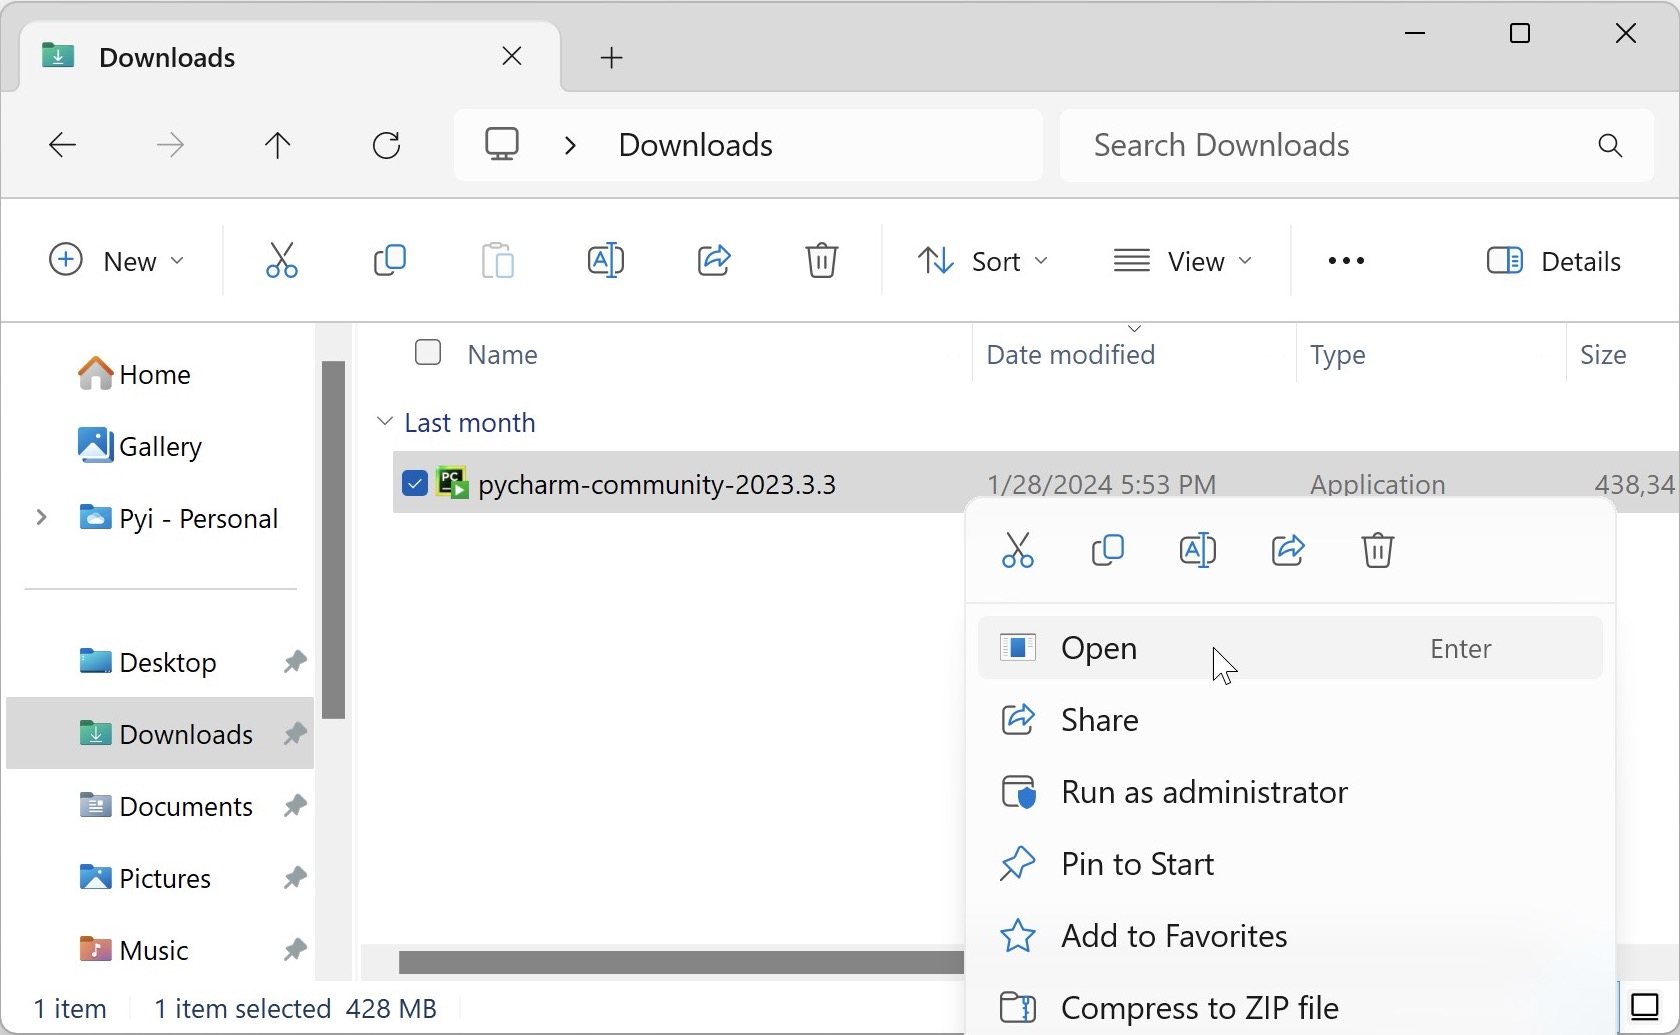
\includegraphics[width=.88\textwidth, trim={2.4mm 12cm 2mm 2mm},clip]{images/pycharm_install/2.jpg}};
    \drawshadow{image}
\end{tikzpicture}
\caption{} 
\label{fig:opnpychminstlr}
\end{figure}

\fEn{\mytcboxinl{PyCharm Community Edition}} ကို ဒေါင်းလုဒ်လုပ်ပါ။ (ဝဘ်စာမျက်နှာ အပေါ်ပိုင်းက ဝယ်သုံးရတဲ့ \fEn{\mytcboxinl{PyCharm Professional}} ကို ဒေါင်းလုဒ် မှားမလုပ်မိဖို့ သတိပြုပါ)။ အင်စတော်လာဖိုင်ကို ညာကလစ်နှိပ်ပြီး \fEnSnd{Open} လုပ်ပါ (ပုံ \fRefNo{\ref{fig:opnpychminstlr}} ကိုကြည့်ပါ)။ \fEnSnd{Yes/No} မေးတဲ့အခါ \fEnSnd{Yes} နှိပ်ပါ။ \mytcboxinl{\fEnSnd{Next >}} ကို နှိပ်၍ ရှေ့ကိုဆက်သွားပြီး နောက်ဆုံးမှာ \mytcboxinl{\fEnSnd{Install}} နှိပ်ပြီး ကွန်ဖန်းလုပ်ပါ။ အင်စတောလ်ပြီးသွားရင် \mytcboxinl{\fEnSnd{Finish}} နှိပ်ပါ။

ဝင်းဒိုး \fEnSnd{Taskbar Search} ကနေ \fEn{PyCharm} ကိုရှာပြီးဖွင့်ပါ (ပုံ \fRefNo{\ref{fig:schpychm}} ကို ကြည့်ပါ)။ သဘောတူကြောင်း ကွန်းဖန်းလုပ်ခိုင်းရင် ချက်ခ်ဘောက်စ် ချက်ခ်လုပ်ပြီး \mytcboxinl{\fEnSnd{Continue}} နှိပ်ပါ။  ဒေတာပို့ချင်လား ထပ်မေးပါလိမ့်မယ်။ \mytcboxinl{\fEnSnd{Don't Send}} နှိပ်ပါ။ \fEnSnd{Welcome} စခရင်ကိုပေါ်လာမယ်။ ပုံ (\fRefNo{\ref{fig:pychmwlcm}}) မှာ ကြည့်ပါ။




\todo{youtube facebook လင့်ထည့်ရန်}

\begin{mytcbox}
ဒီစာရေးနေချိန် လက်ရှိ \fEn{PyCharm} ဗားရှင်းက ၂၀၂၃ ပါ။ သိပ်မကြာခင် ၂၀၂၄ ထွက်ပါတော့မယ်။ အကယ်၍ လက်ရှိဗားရှင်းထက် နိမ့်တဲ့ဗားရှင်းတွေကို ဒေါင်းလုဒ် လုပ်ချင်ရင် အောက်ပါ လင့်ကို သွားပါ။ 
%
\begin{minted}[frame=lines, framerule=0pt]{text}
https://www.jetbrains.com/pycharm/download/other.html
\end{minted}
%
ဗားရှင်း ၂၀၂၄/၂၅ ထွက်ပြီးတဲ့ အချိန်မှာ ၂၀၂၃ ဗားရှင်းကို လိုချင်ရင် ဝဘ်စာမျက်နှာမှ ရှာပြီး ဒေါင်းလုဒ် လုပ်ပါ။ ၂၀၂၃ မှာလည်း ဗားရှင်းအခွဲတွေ ရှိပါသေးတယ်။ လက်ရှိအမြင့်ဆုံး ဗားရှင်းအခွဲ (ဥပမာ ၂၀၂၃.၃.၃) ကို သုံးလို့ရပါတယ်။ ၂၀၂၄/၂၅ သုံးမယ်ဆိုရင်လည်း ပြဿနာတော့ မရှိပါဘူး။ \fEn{Update} ဗားရှင်းဖြစ်တဲ့အတွက် ပုံတွေမှာ ပြထားတာနဲ့တော့ ကွာခြားချက်တချို့ ရှိကောင်းရှိနိုင်ပါတယ်။
\end{mytcbox}
%

\begin{figure}[tbh!]
\begin{tikzpicture}
    \node[anchor=south west,inner sep=0] (image) at (0,0)
        {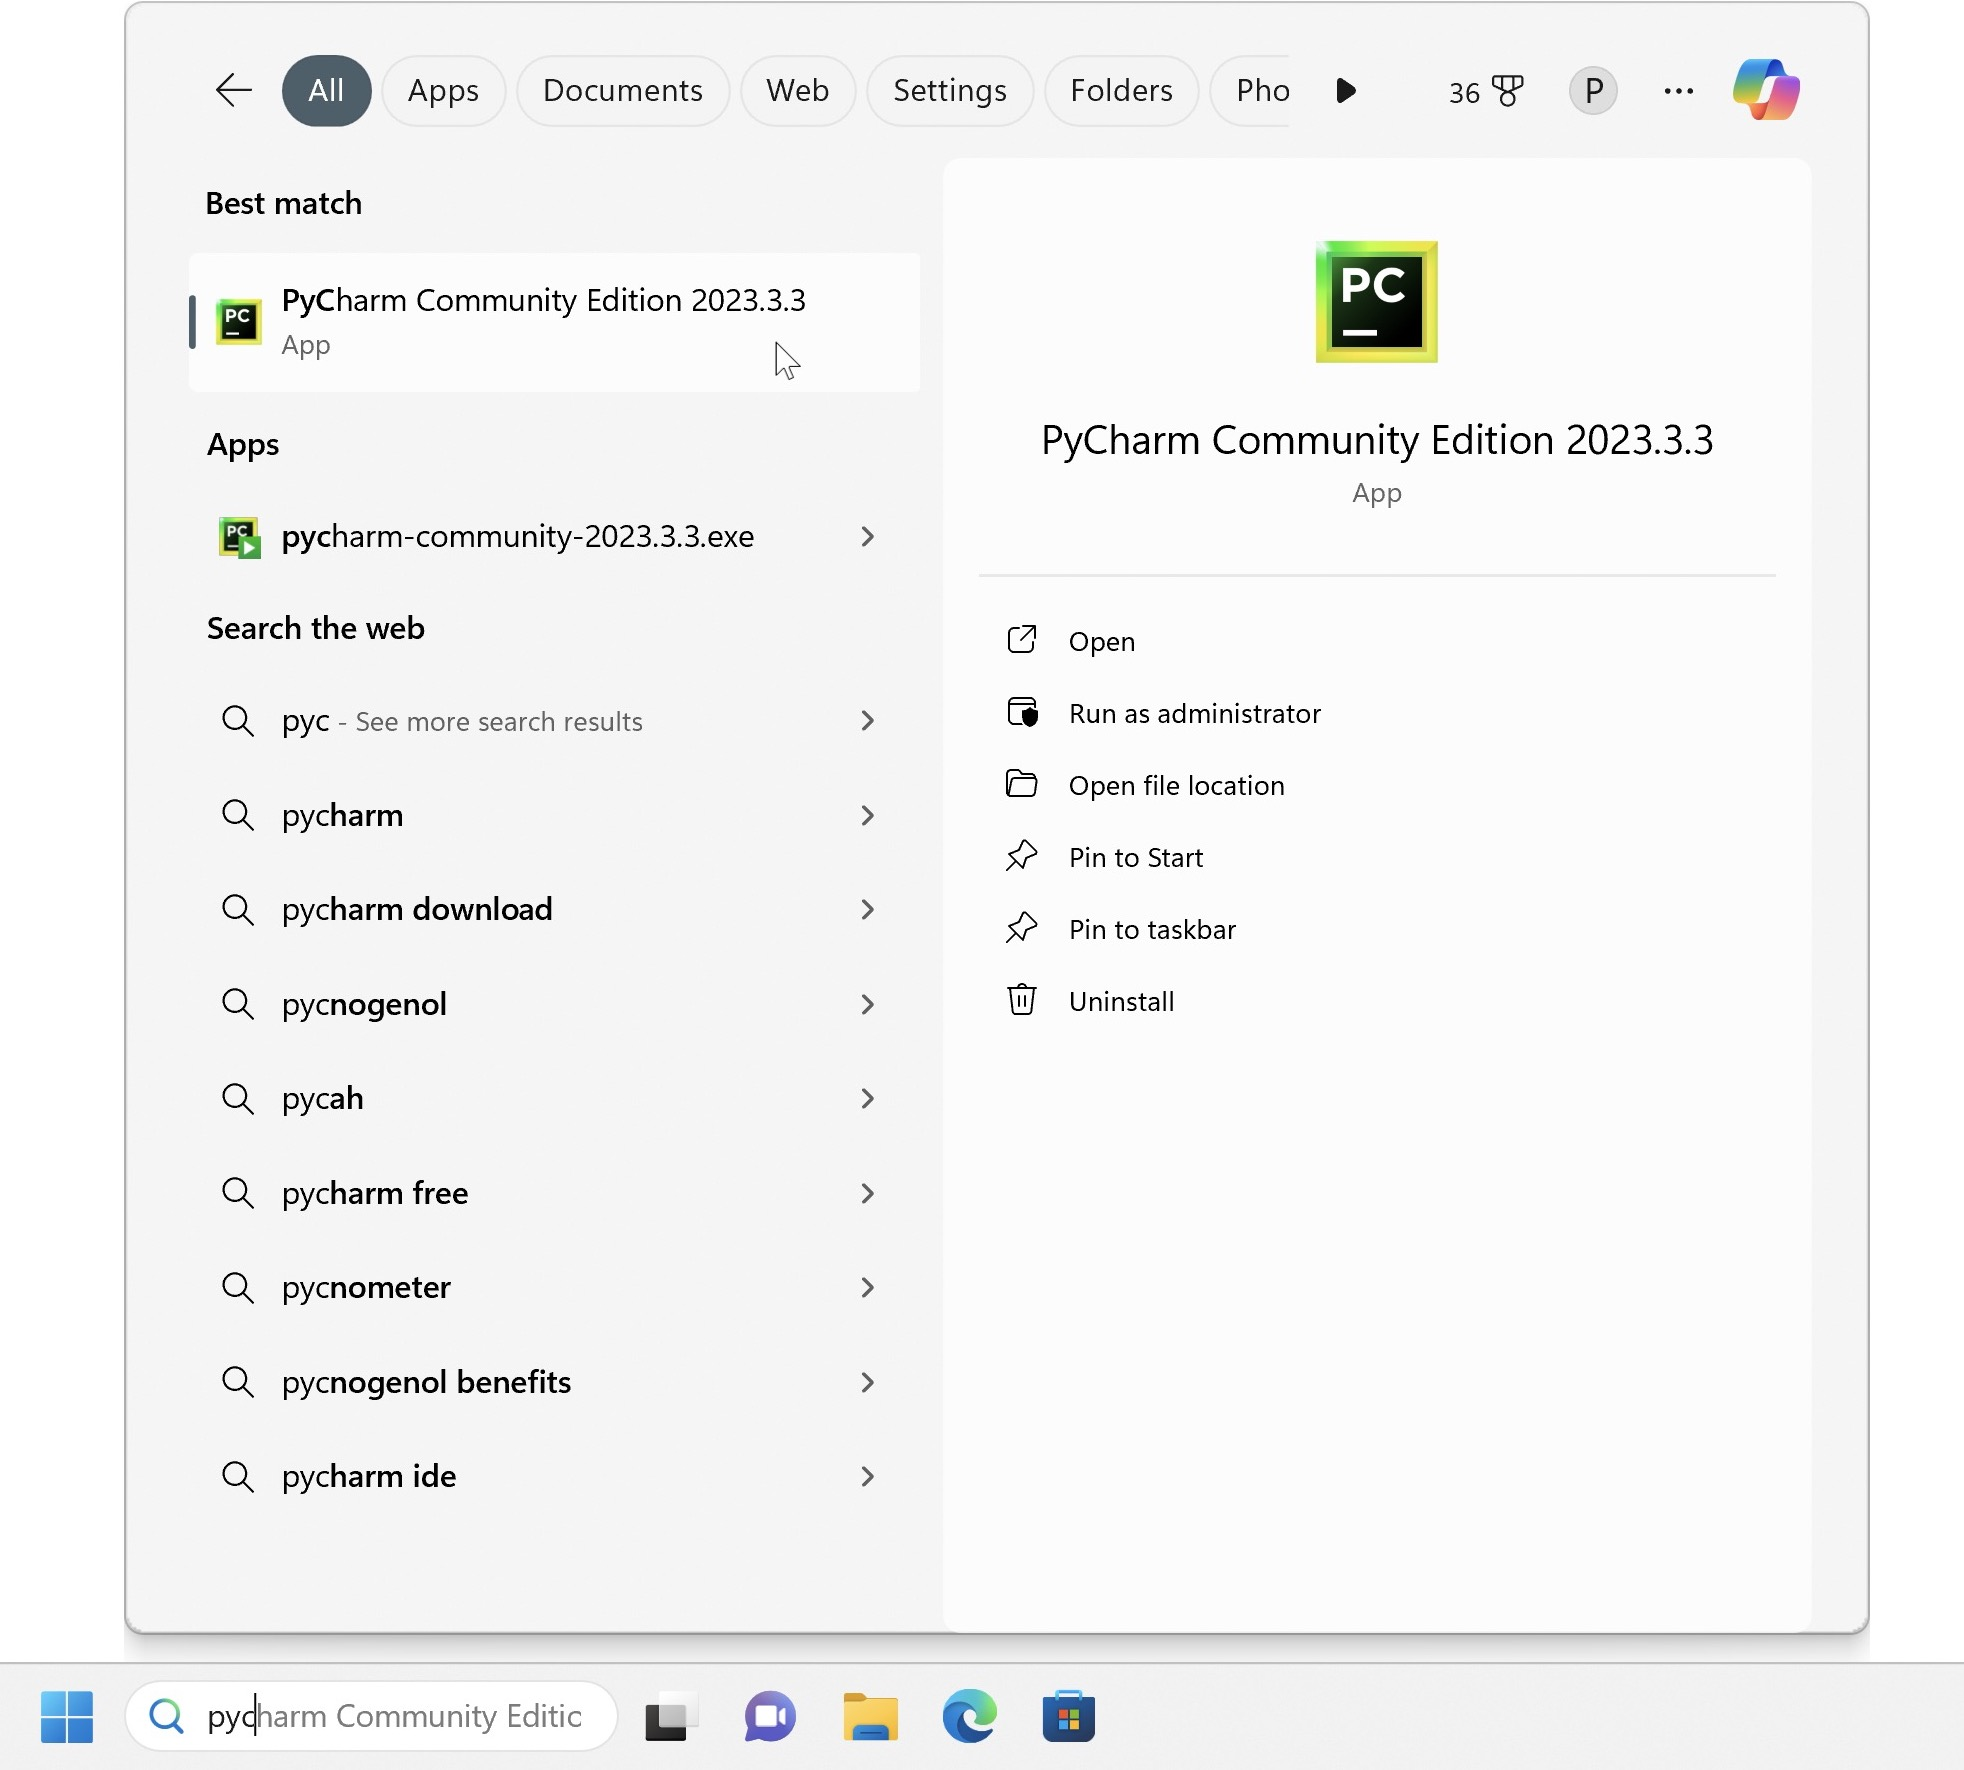
\includegraphics[width=.9\textwidth, trim={2.4mm 2mm 2mm 2mm},clip]{images/pycharm_install/3.jpg}};
    \drawshadow{image}
\end{tikzpicture}
\caption{} 
\label{fig:schpychm}
\end{figure}

\begin{figure}[H]
\begin{tikzpicture}
    \node[anchor=south west,inner sep=0] (image) at (0,0)
        {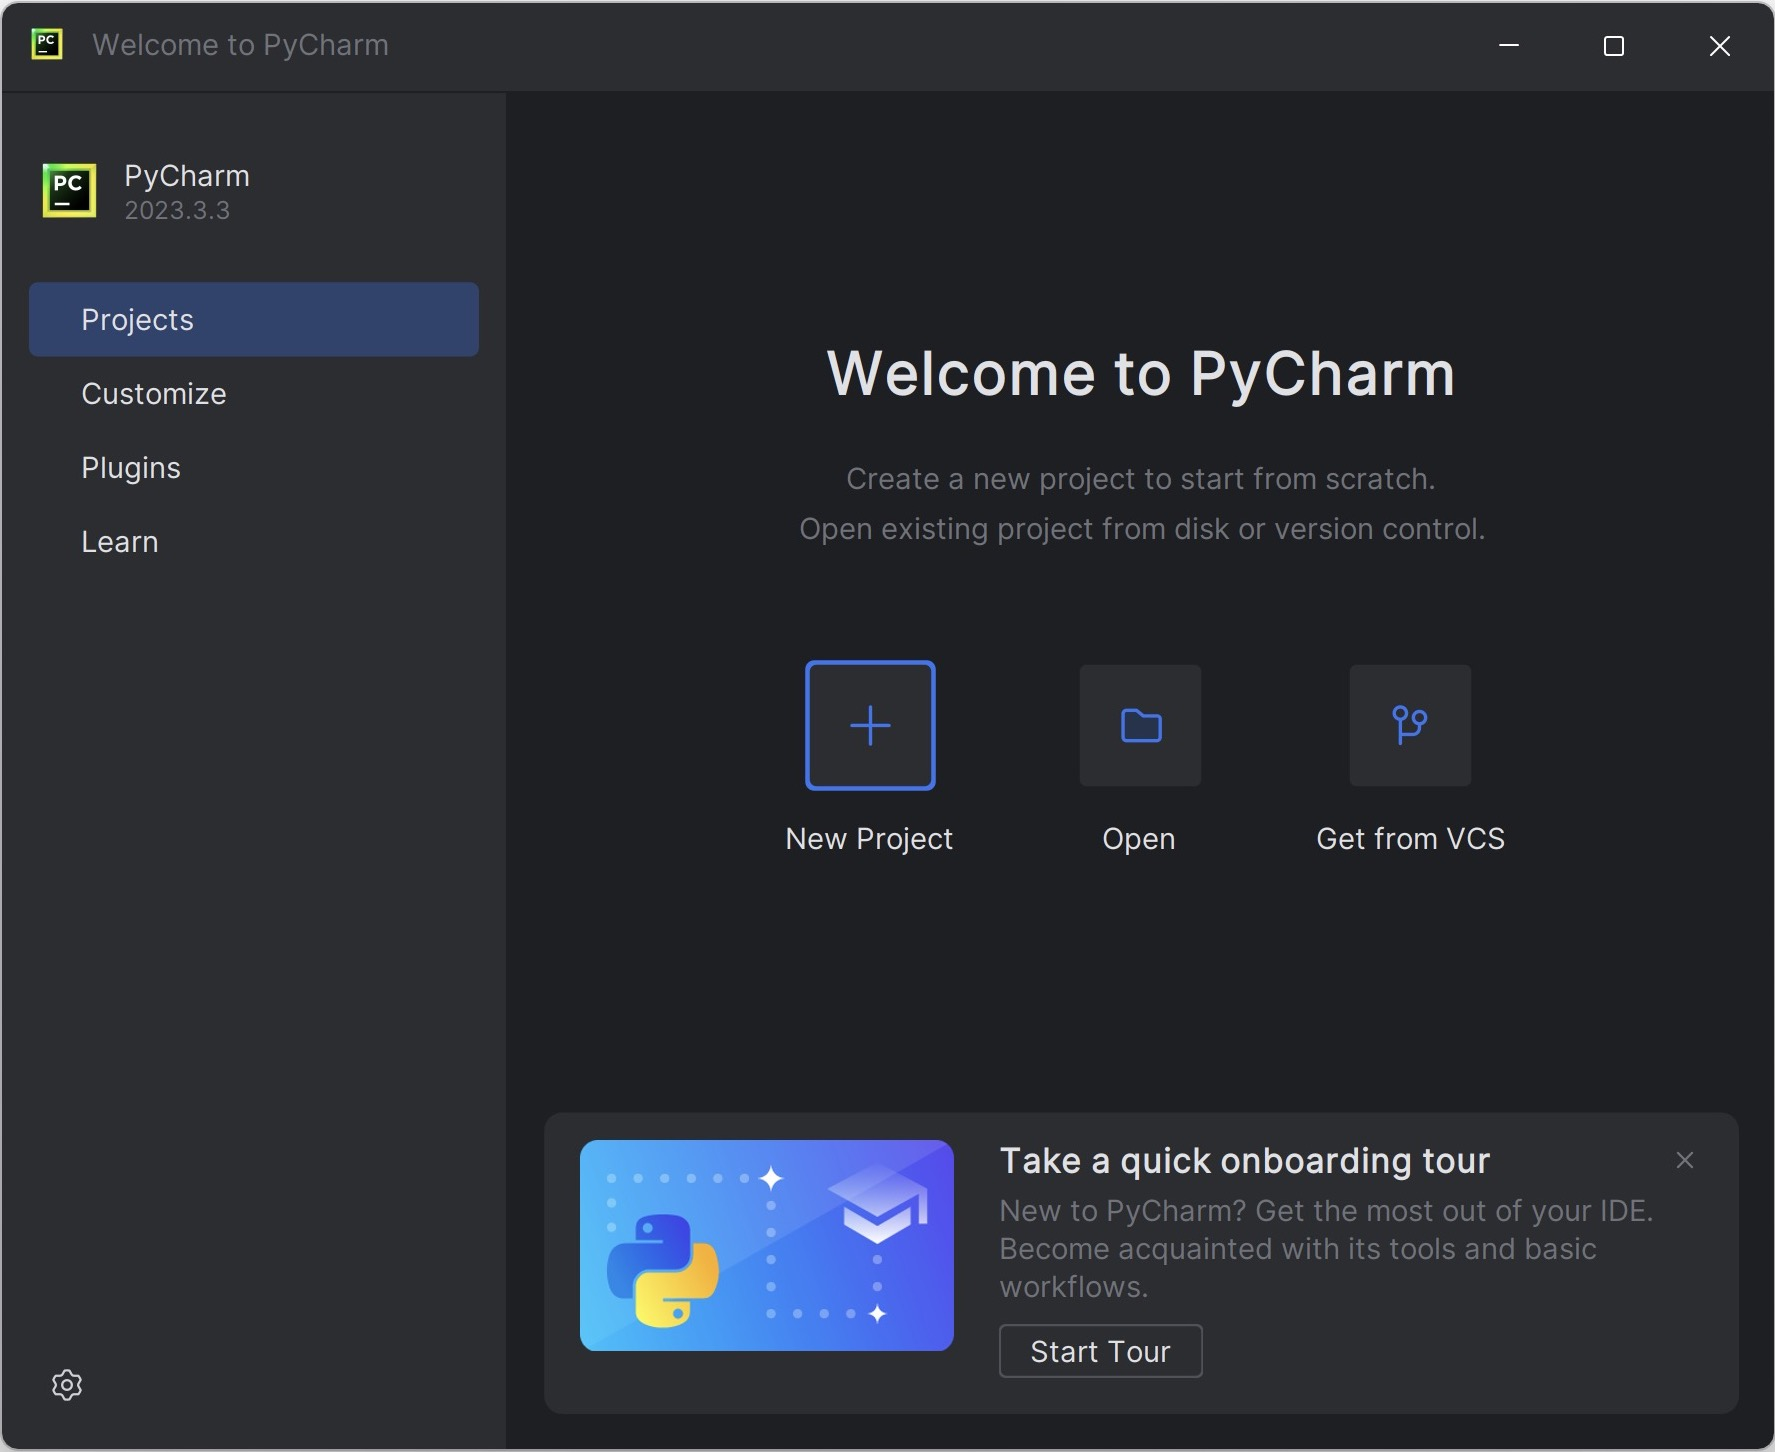
\includegraphics[width=.98\textwidth, trim={2.4mm 2mm 2mm 2mm},clip]{images/pycharm_install/4.jpg}};
    \drawshadow{image}
\end{tikzpicture}
\caption{} 
\label{fig:pychmwlcm}
\end{figure}

\subsection*{PyCharm IDE ဆိုတာဘာလဲ}
\fEn{PyCharm} ဟာ \fEn{Python} နဲ့ ဆော့ဖ်ဝဲ  ရေးဖို့အတွက် အထောက်အကူပြု \fEn{Integrated Development Environment(IDE)} ဆော့ဖ်ဝဲဖြစ်ပါတယ်။ စာစီစာရိုက်လုပ်တဲ့အခါ \fEn{Microsoft Word} ကို အသုံးပြုကြသလိုပဲ \fEn{Python} ကုဒ်ရေးဖို့ \fEn{PyCharm} ကိုသုံးတဲ့ သဘောပေါ့။ \fEn{PyCharm IDE} က \fEn{Python} ပရောဂျက်တွေ အတွက် အဓိကရည်ရွယ်တယ်။ အဆောက်အဦးတစ်ခု၊ တံတားတစ်ခု ဆောက်လုပ်တာကို ပရောဂျက်လို့ ပြောလေ့ရှိသလို ပရိုဂရမ်/ဆော့ဖ်ဝဲတစ်ခု တည်ဆောက်တာကိုလည်း ပရောဂျက်လို့ပဲ သုံးနှုန်းပါတယ်။ တစ်ဦးတစ်ယောက်တည်း ရေးတဲ့ ပရိုဂရမ်အသေးလေးတွေ အတွက် \fEn{PyCharm} ကို အသုံးပြုနိုင်သလို ပရိုဂရမ်မာတွေ အဖွဲ့လိုက်နဲ့ တည်ဆောက်ရတဲ့ ပရောဂျက်ကြီးတွေ အတွက်လည်း သုံးပါတယ်။ ဒီစာအုပ်မှာတော့ \fEn{PyCharm} ရဲ့ အဆင့်မြင့်ဖီချာတွေကို အသုံးပြုမှာ မဟုတ်ပါဘူး။ ပရိုဂရမ်းမင်း စလေ့လာသူတွေကို လွယ်ကူအဆင်ပြေစေတဲ့ အခြေခံ ဖီချာတွေလောက်ပဲ အသုံးပြုမှာပါ။ 

\clearpage

\subsection*{PyCharm ပရောဂျက်ဆောက်ခြင်း}
အင်စတောလ်လုပ်ပြီးရင် \fEn{PyCharm IDE} ကိုဖွင့်ပြီး \fEnSnd{Welcome} စခရင်မှ သိုမဟုတ် \fEnSnd{File} မီနူးမှ \fEnSnd{New Project} နှိပ်ပြီး ပရောဂျက် အသစ်ယူပါ (ပြီးခဲတဲ့ ပုံ \fRefNo{\ref{fig:pychmwlcm}} ကို ပြန်ကြည့်ပါ)။ နံမည်ကို \fEnSnd{MeetKarel} ပေးပါ။ ပုံ (\fRefNo{\ref{fig:new_proj}}) မှာ တွေ့ရတဲ့အတိုင်း \fEnSnd{\mytcboxinl{Pure Python}, \mytcboxinl{Proj venv}} နဲ့ \fEn{Python} ဗားရှင်း \fEnSnd{3.12.xx} ကို ရွေးပါ။ \fEnSnd{xx} က အခြားဂဏန်း ဖြစ်နေနိုင်တယ်။ အဓိက ဗားရှင်း \fEnSnd{3.12} သာ ဖြစ်ပါစေ။ \fEnSnd{Create} ခလုတ်နှိပ်ပါ။ ပရောဂျက်အတွက် \fEn{Python} ကို အင်စတောလ် လုပ်ပါလိမ့်မယ်။

မိမိလေ့လာနေတဲ့ အခန်းတစ်ခန်းချင်းစီအတွက် ပရောဂျက်တစ်ခု ဆောက်နိုင်ပါတယ်။ အခန်း (၂) အတွက် \fEnSnd{Chapter02} ၊ အခန်း (၃) အတွက် \fEnSnd{Chapter03} စသည်ဖြင့်။  သက်ဆိုင်ရာအခန်းအလိုက် ကုဒ်ဖိုင်တွေကို ပရောဂျက်တစ်ခုစီမှာ ထားတဲ့အတွက် ဖိုင်တွေများပြီး ရှုပ်ထွေဖောင်းပွနေတဲ့ ပြဿနာ မရှိတော့ဘူး။ ကုဒ်ဖိုင်တွေကို ပရောဂျက်တစ်ခုထဲမှာပဲ ဖိုဒါအလိုက်ခွဲထားလို့ရပေမဲ့ စလေ့လာသူအနေနဲ့ ပရောဂျက်တစ်ခုချင်း ခွဲထားတာလောက် မလွယ်ကူဘူး။

ပရောဂျက် အသစ်ယူတဲ့အခါ တည်နေရာ \mytcboxinl{\fEnSnd{Location:}} ကို သူ့နဂိုအတိုင်း ထားနိုင်သလို မိမိထားချင်တဲ့နေရာကို ညာဘက်စွန်း ဖိုဒါအိုင်ကွန်လေးနှိပ်ပြီး ပြောင်းလို့ရတယ်။

\begin{figure}[tb!]
\begin{tikzpicture}
    \node[anchor=south west,inner sep=0] (image) at (0,0)
        {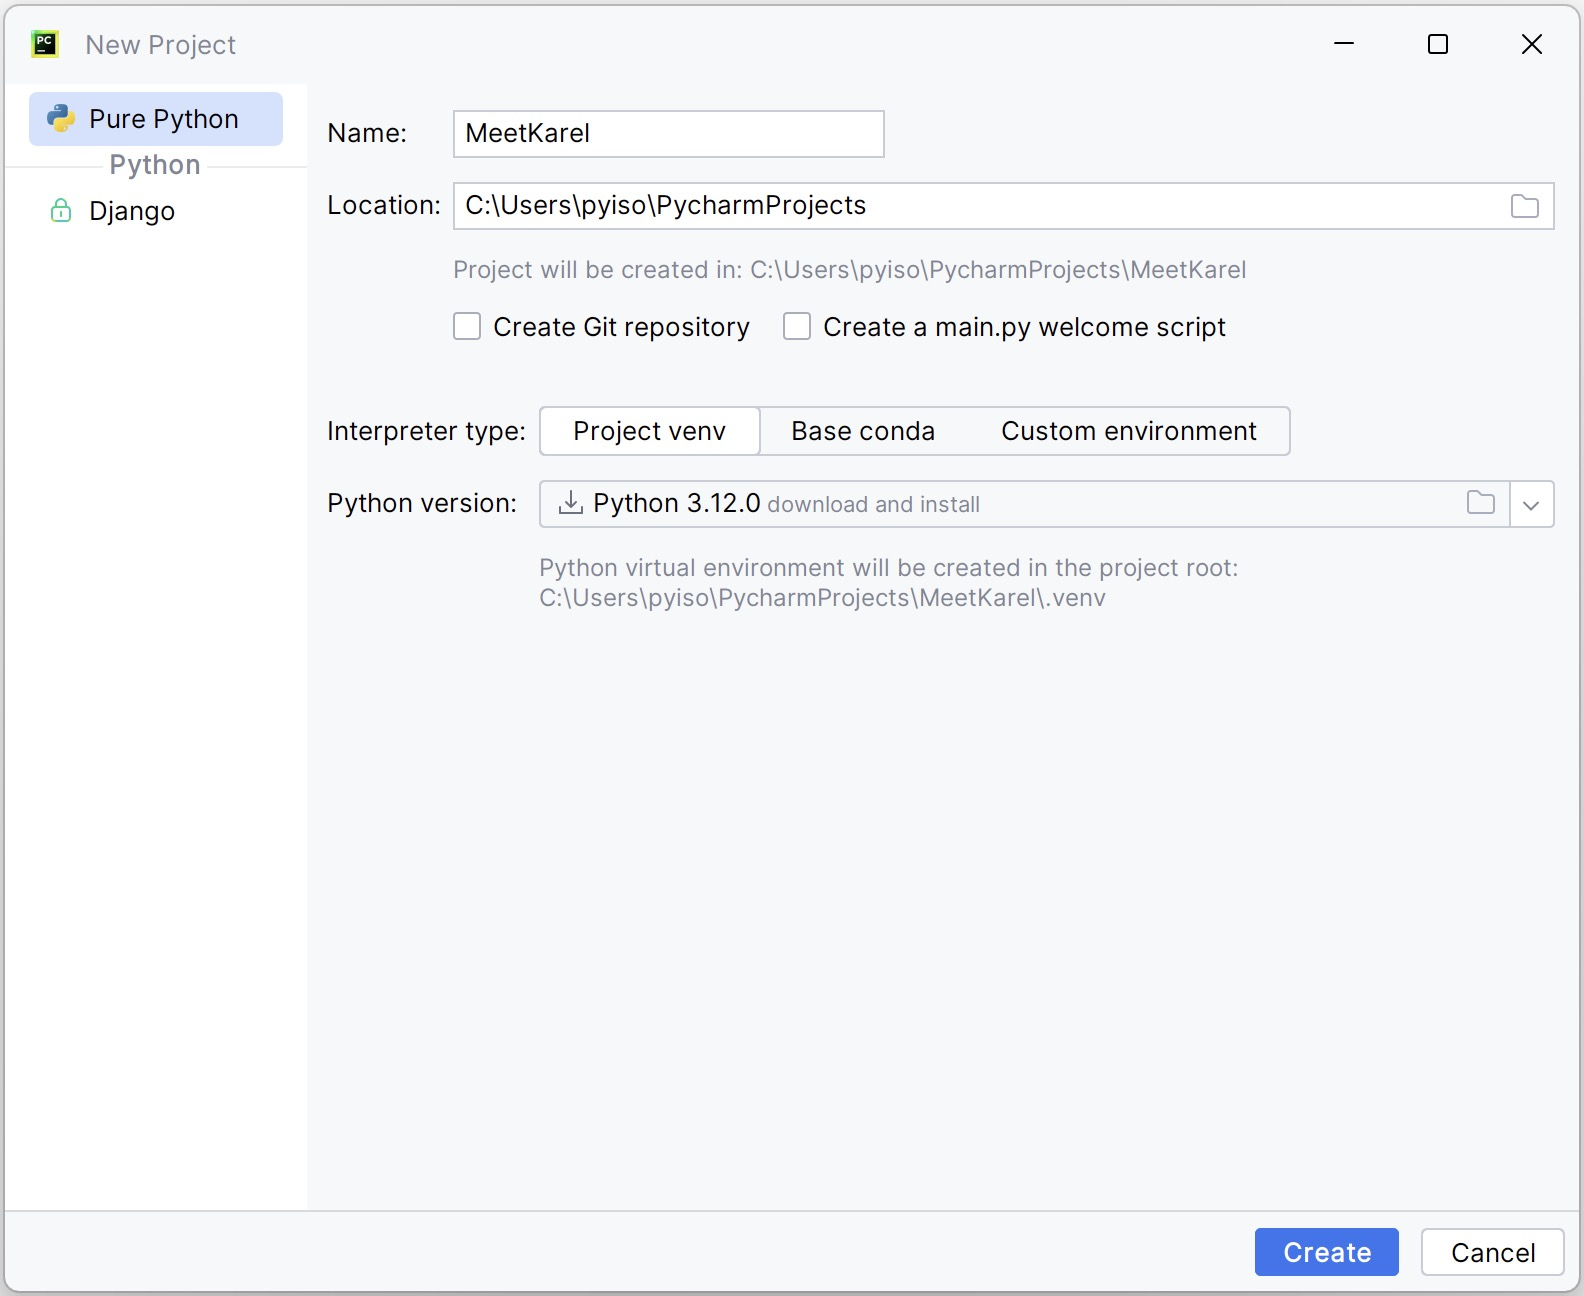
\includegraphics[width=.98\textwidth, trim={2.3mm 2mm 2mm 2.3mm},clip]{images/pycharm_install/new_proj.jpg}};
    \drawshadow{image}
    \draw [draw=red,very thick,rounded corners] (0.15,9.82) rectangle (2.3,9.31);
    \draw [draw=red,very thick,rounded corners] (4.3,7.27) rectangle (6.21,6.76);
    \draw [draw=red,very thick,rounded corners] (4.3,6.68) rectangle (8,6.17);

\end{tikzpicture}
\caption{ပရောဂျက် အသစ်ယူခြင်း} 
\label{fig:new_proj}
\end{figure}

\begin{figure}[tb!]
\begin{tikzpicture}
    \node[anchor=south west,inner sep=0] (image) at (0,0)
        {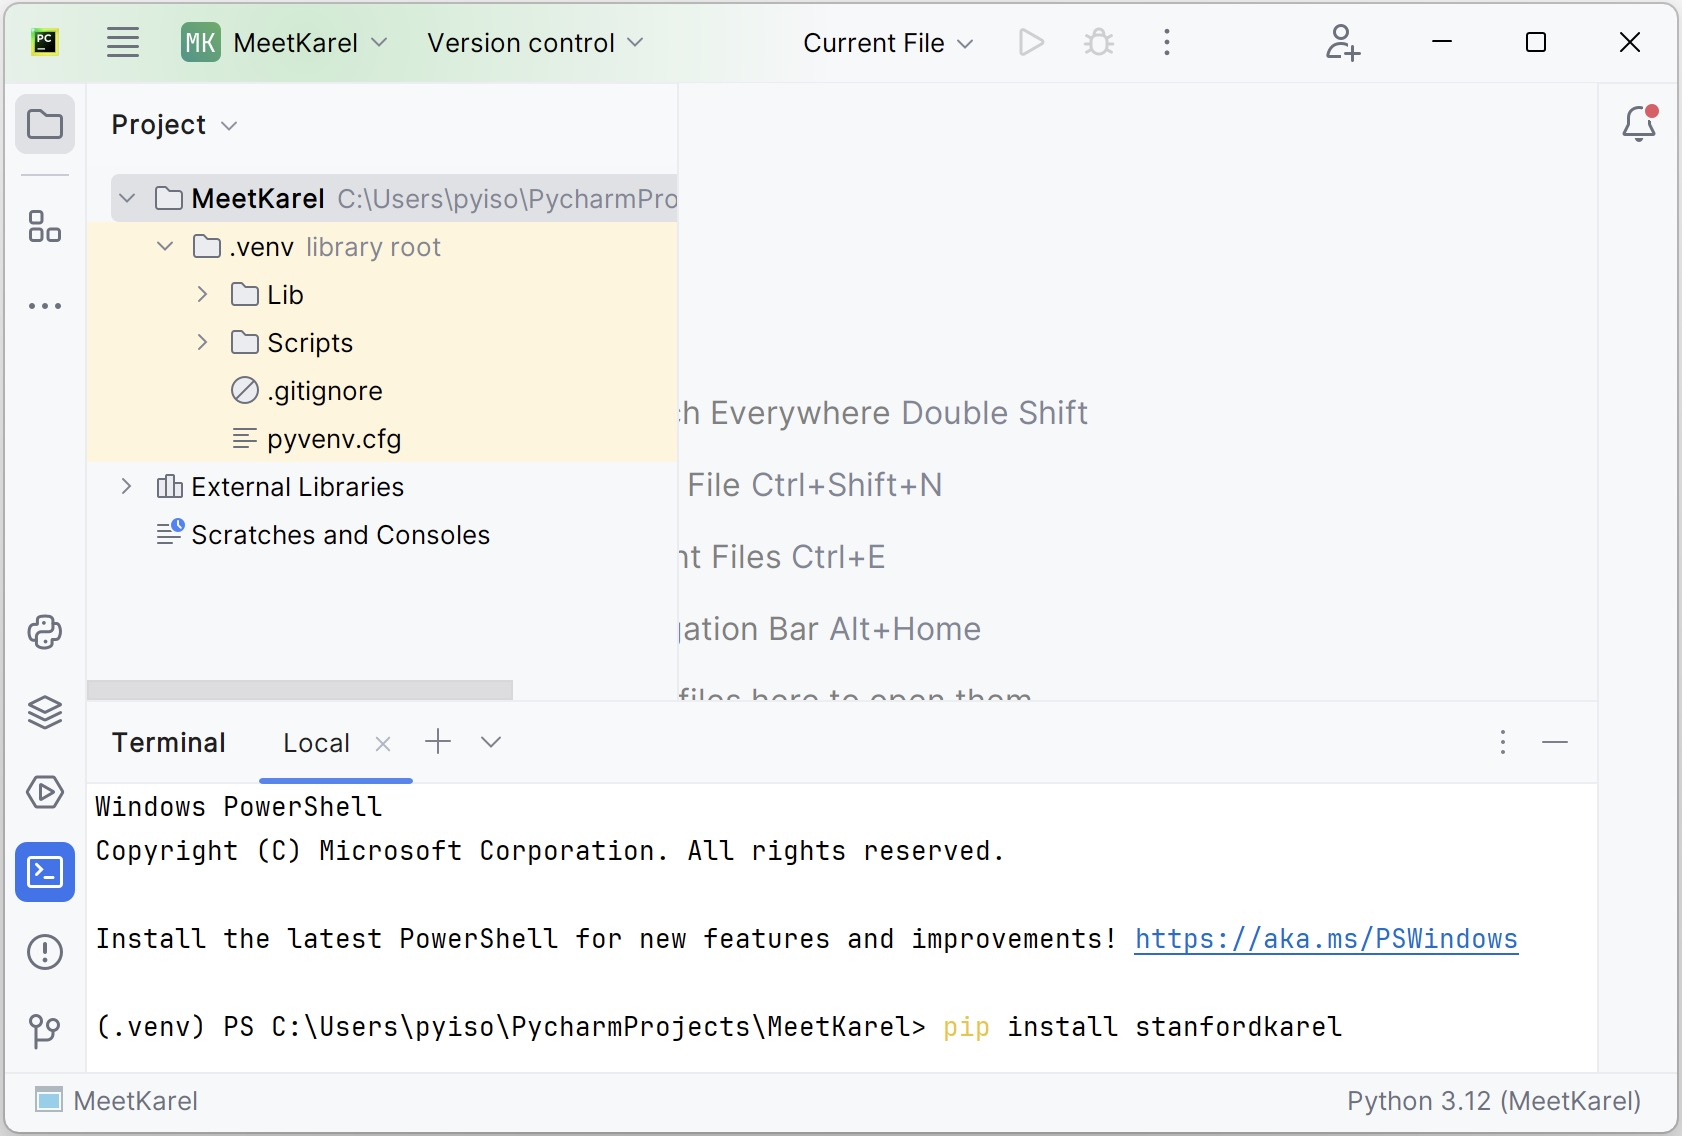
\includegraphics[width=.98\textwidth, trim={2.4mm 2mm 2mm 2.4mm},clip]{images/pycharm_install/install_karel.jpg}};
    \drawshadow{image}
    \draw [draw=red,very thick,rounded corners] (0.02,2.26) rectangle (0.57,1.71);
    \draw [draw=red,very thick,rounded corners] (7.13,1.1) rectangle (10.4,0.55);
\end{tikzpicture}
\caption{Karel လိုက်ဘရီ အင်စတောလ်လုပ်ခြင်း} 
\label{fig:install_karel}
\end{figure}

\subsection*{stanfordkarel လိုက်ဘရီ အင်စတောလ်လုပ်ခြင်း}
ပုံ (\fRefNo{\ref{fig:install_karel}}) မှာ အနီရောင် ဝိုင်းပြထားတဲ့ အိုင်ကွန်ကို နှိပ်ပြီး \fEnSnd{Terminal} ကိုဖွင့်ပါ။ \fEnSnd{Terminal} မှာ အောက်ပါ ကွန်မန်းဖြင့် 
%
\begin{minted}[frame=lines, framerule=0pt]{text}
pip install stanfordkarel
\end{minted}
%
ကားရဲလ်လိုက်ဘရီကို အင်စတောလ်လုပ်ပါ။ ပုံ (\fRefNo{\ref{fig:install_karel}}) မှာ  အနီရောင် ဝိုင်းပြထားပါတယ်။ ခဏကြာတဲ့အခါ အခုလို \fOpn{မက်ဆေ့ချ်}တွေ ကျလာပါလိမ့်မယ်။ 

%
\begin{minted}[frame=lines, framerule=0pt,escapeinside=ßß]{text}
Collecting stanfordkarel
  Downloading stanfordkarel-0.2.7-py3-none-any.whl (51 kB)
     ━━━━━━━━━━━━━━━━━━━━━━━━━━━━━━━━━━━━━━━━ 51.9/51.9 kB 443.1 kB/s 
    eta 0:00:00
Installing collected packages: stanfordkarel
ß\colorbox{yellow}{Successfully installed stanfordkarel-0.2.7}ß

[notice] A new release of pip is available: 23.2.1 -> 24.0
[notice] To update, run: python.exe -m pip install --upgrade pip
(.venv) PS C:\Users\pyiso\PycharmProjects\MeetKarel>
\end{minted}
%
ဟိုက်လိုက်ပြထားတဲ့ \fOpn{မက်ဆေ့ချ်} တွေ့ရရင် အင်စတောလ်လုပ်တာ အောင်မြင်လို့ပါ။

\begin{mytcbox}
မှတ်ချက်။\qquad ။ ပရောဂျက် အသစ်ဆောက်တိုင်း လိုအပ်တဲ့ လိုက်ဘရီကို တစ်ခါထပ်ပြီး အင်စတောလ် လုပ်ရပါမယ်။ ကားရဲလ်အခန်း ပရောဂျက်တစ်ခုစီအတွက် \fEnSnd{stanfordkarel} လိုက်ဘရီကို အထက်ဖော်ပြပါအတိုင်း အင်စတောလ် လုပ်ဖို့လိုတယ်။
\end{mytcbox}

\clearpage
\subsection*{နမူနာ ကားရဲလ် ကမ္ဘာနှင့် ပရိုဂရမ်ကုဒ် ဖိုင်များထည့်ခြင်း}
\fEnSnd{meet\_karel.zip} ဖိုင်ကို \todo{ဒေါင်းလုဒ်လင့်ထည့်ရန်} ဒီလင့် \fCode{http://tinyurl.com/3mmm9c7j} ကနေ ဒေါင်းလုဒ်လုပ်ပါ။ ၎င်း \fEnSnd{zip} ဖိုင်ကို \fEn{extract} လုပ်ပါ။ \fEnSnd{meet\_karel} နံမည်နဲ့ ဖိုဒါတစ်ခု ရလာပါမယ်။ ၎င်းဖိုဒါထဲမှ အောက်ပါ \fEnSnd{worlds} ဖိုဒါနှင့် \fEnSnd{.py} ဖိုင်အားလုံးကို ကော်ပီလုပ်ပါ။ 
%
\begin{itemize}
    \item \fEnSnd{worlds} 
    \begin{itemize}
        \item \fEnSnd{meet\_karel.w}
        \item \fEnSnd{move\_beeper\_to\_other\_side.w}
    \end{itemize}
    \item \fEnSnd{meet\_karel.py}
    \item \fEnSnd{move\_beeper\_to\_other\_side.py}
    \item \fEnSnd{world\_editor.py}
\end{itemize}
%

\fEnSnd{MeetKarel} ပရောဂျက်ထဲတွင် ကူးထည့်ပါ။ ပင်မ ပရောဂျက် \fEnSnd{MeetKarel} (ပုံ \fRefNo{\ref{fig:edit_meet_karel}} မှာ မြှားပြထား) ပေါ်မှာ ညာကလစ်နှိပ်ပြီး \fEnSnd{Paste} လုပ်ရမှာပါ။ ကော်ပီကူးထည့်လိုက်တဲ့ ဖိုင်တွေက ပုံမှာ တွေ့ရတဲ့အတိုင်း  \fEnSnd{MeetKarel} ဖိုဒါအောက်မှာ ရှိသင့်ပါတယ်။

\begin{mytcbox}
အခန်းအလိုက် နမူနာ ကုဒ်ဖိုင်တွေ ထည့်ပေးထားတဲ့ \fEnSnd{.zip} ဖိုင်တွေကိုလည်း အထက်ပါအတိုင်း အလားတူ လုပ်ရပါမယ်။ ပရောဂျက်အသစ်ဆောက်၊ \fEnSnd{.zip} ဖိုင်ကို ဖြည်၊ ရလာတဲ့ ဖိုဒါထဲက ဖိုင်တွေကို ပင်မ ပရောဂျက် ဖိုဒါထဲ ကော်ပီကူးထည့် ရုံပါပဲ။
\end{mytcbox}

\fEnSnd{meet\_karel.py} ဖိုင်ကို ကလစ်နှစ်ချက်နှိပ် ဖွင့်ပါ။ ပုံ (\fRefNo{\ref{fig:edit_meet_karel}}) မှာ အနီဝိုင်းထားတဲ့  ကုဒ်အယ်ဒီတာ \fEn{(code editor)} ပွင့်လာပါမယ်။ အဲဒီ မူရင်းဖိုင်မှာ အောက်ပါအတိုင်း ဆက်လက် ပြင်ဆင်ဖြည့်စွက်ပါ။
%
\setlength{\fboxsep}{0pt}
\label{lst:mtkrl}
\begin{minted}[frame=\mintframe, framerule=\mintrule,framesep= \mintsep, xleftmargin=\xlftmargin
                , bgcolor=mintbgcolor,rulecolor=mintrulecolor
                , python3=true]{python}
from stanfordkarel import *


def main():
    """Karel code goes here!"""
    move()
    move()
    move()
    pick_beeper()
    turn_left()
    move()
    move()

    turn_left()
    turn_left()
    turn_left()

    move()
    put_beeper()


if __name__ == "__main__":
    run_karel_program("meet_karel")
\end{minted}
%

%http://tinyurl.com/3mmm9c7j
%https://bit.ly/42MhViS

% google drive root folder
%http://tinyurl.com/mkamnasm
%https://bit.ly/3T3tgrA

\begin{mytcbox}
\fEn{run} ထားတဲ့ ပရိုဂရမ်တစ်ခုကို တစ်ခါထပ် \fEn{run} ရင် \mytcboxinl{\fEnSnd{Cancel}} (သို့) \mytcboxinl{\fEnSnd{Stop and Rerun}} လုပ်မှာလားမေးတယ်။ \mytcboxinl{\fEnSnd{Stop and Rerun}} လုပ်ရပါတယ်။
\end{mytcbox}

\fEnSnd{meet\_karel.py} ဖိုင်ကို ညာကလစ်နှိမ်ပြီး \fEnSnd{\mytcboxinl{Run 'meet\_karel'}} လုပ်ပါ (အယ်ဒီတာ ဧရိယာမှာ ညာကလစ်နှိမ်ပြီး \fEnSnd{\mytcboxinl{Run 'meet\_karel'}} လုပ်လို့လည်း ရပါတယ်) ။ ပုံ (\fRefNo{\ref{fig:mtkrlpgm}}) က ကားရဲလ် ပရိုဂရမ် တက်လာရင် \fEnSnd{\mytcboxinl{Run Program}} ခလုတ်ကိုနှိပ်ပါ။ ဘိပါကို ကားရဲလ်က ရွှေ့ပေးပါလိမ့်မယ်။

\begin{figure}[b!]
\begin{tikzpicture}
    \node[anchor=south west,inner sep=0] (image) at (0,0)
        {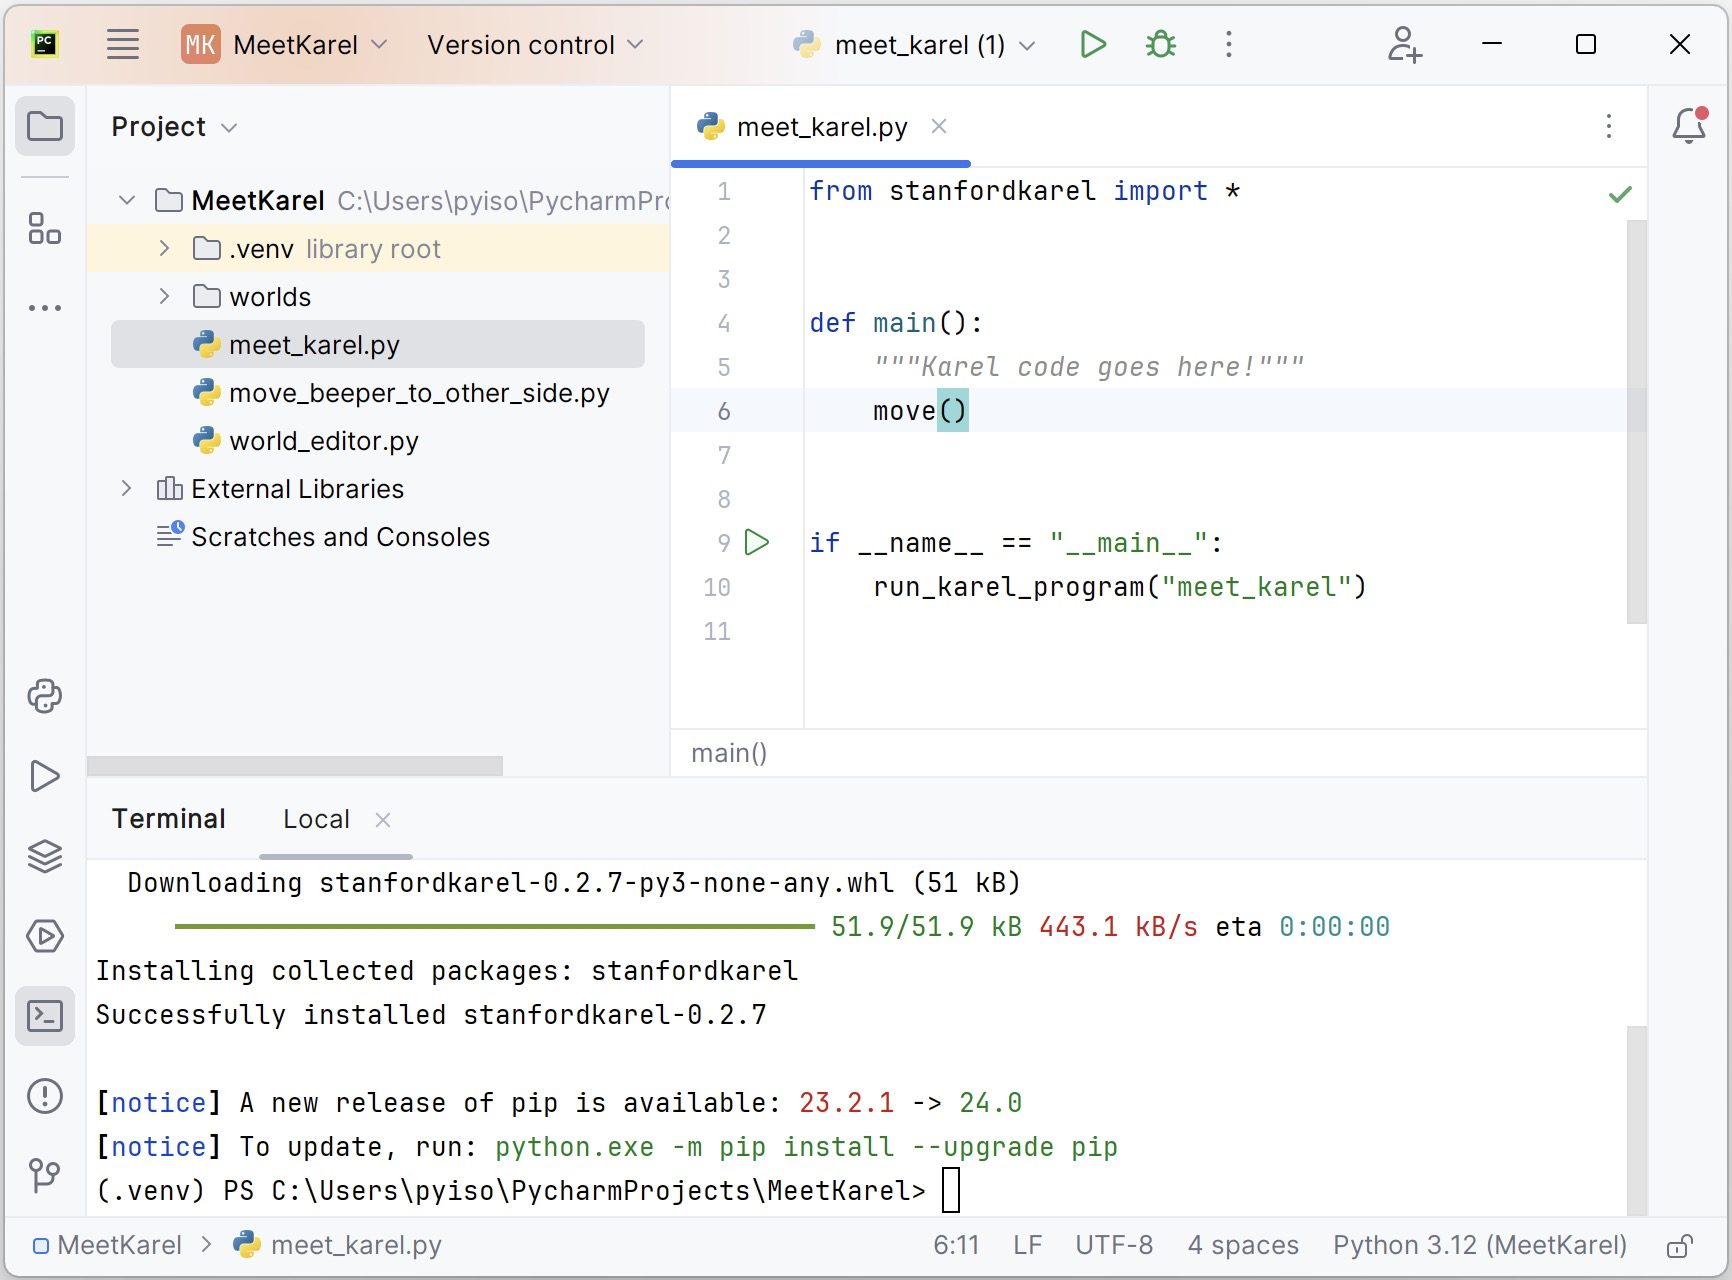
\includegraphics[width=.98\textwidth, trim={2.4mm 2mm 2mm 2.4mm},clip]{images/pycharm_install/edit_meet_karel.jpg}};
    \drawshadow{image}
    
    \draw[-{Latex[length=3mm]}, very thick, red](3, 9)-- (2 ,8.15);
    \draw [draw=red, thick,rounded corners] (5, 8.87) rectangle (12.25 ,3.75);
\end{tikzpicture}
\caption{} 
\label{fig:edit_meet_karel}
\end{figure}


\begin{figure}[b!]
\begin{tikzpicture}
    \node[anchor=south west,inner sep=0] (image) at (0,0)
        {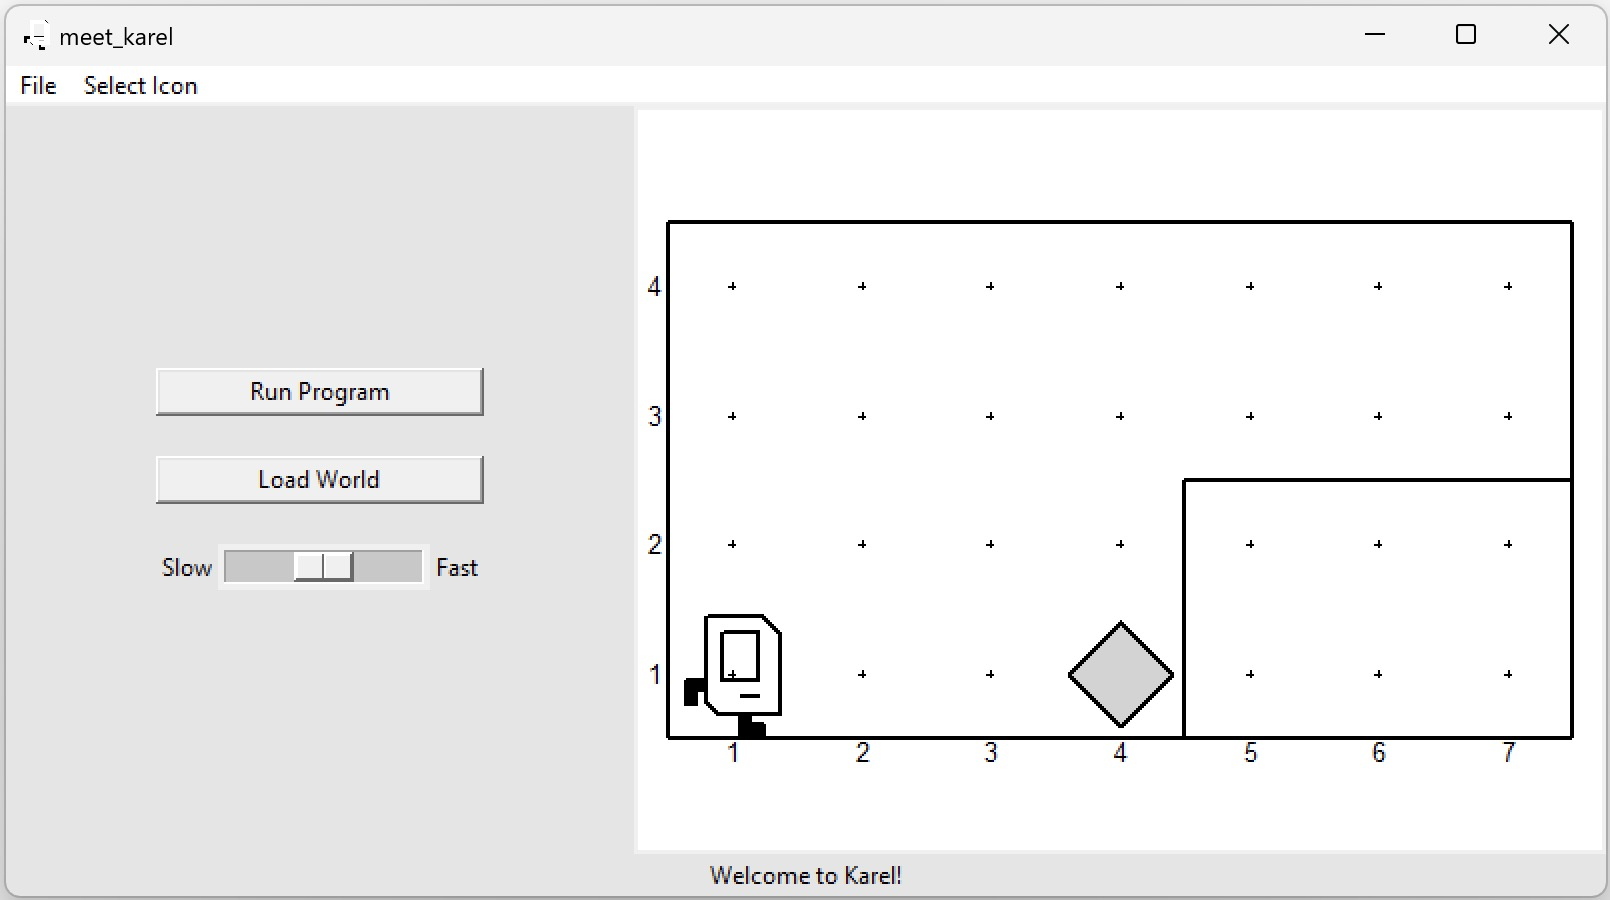
\includegraphics[width=.82\textwidth, trim={2.4mm 2cm 2mm 2mm},clip]{images/pycharm_install/meet_karel_program.jpg}};
    \drawshadow{image}
\end{tikzpicture}
\caption{} 
\label{fig:mtkrlpgm}
\end{figure}



\clearpage
\subsection*{ဆင်းတက်စ်အမှားများ}
\begin{figure}[b!]
\begin{tikzpicture}
    \node[anchor=south west,inner sep=0] (image) at (0,0)
        {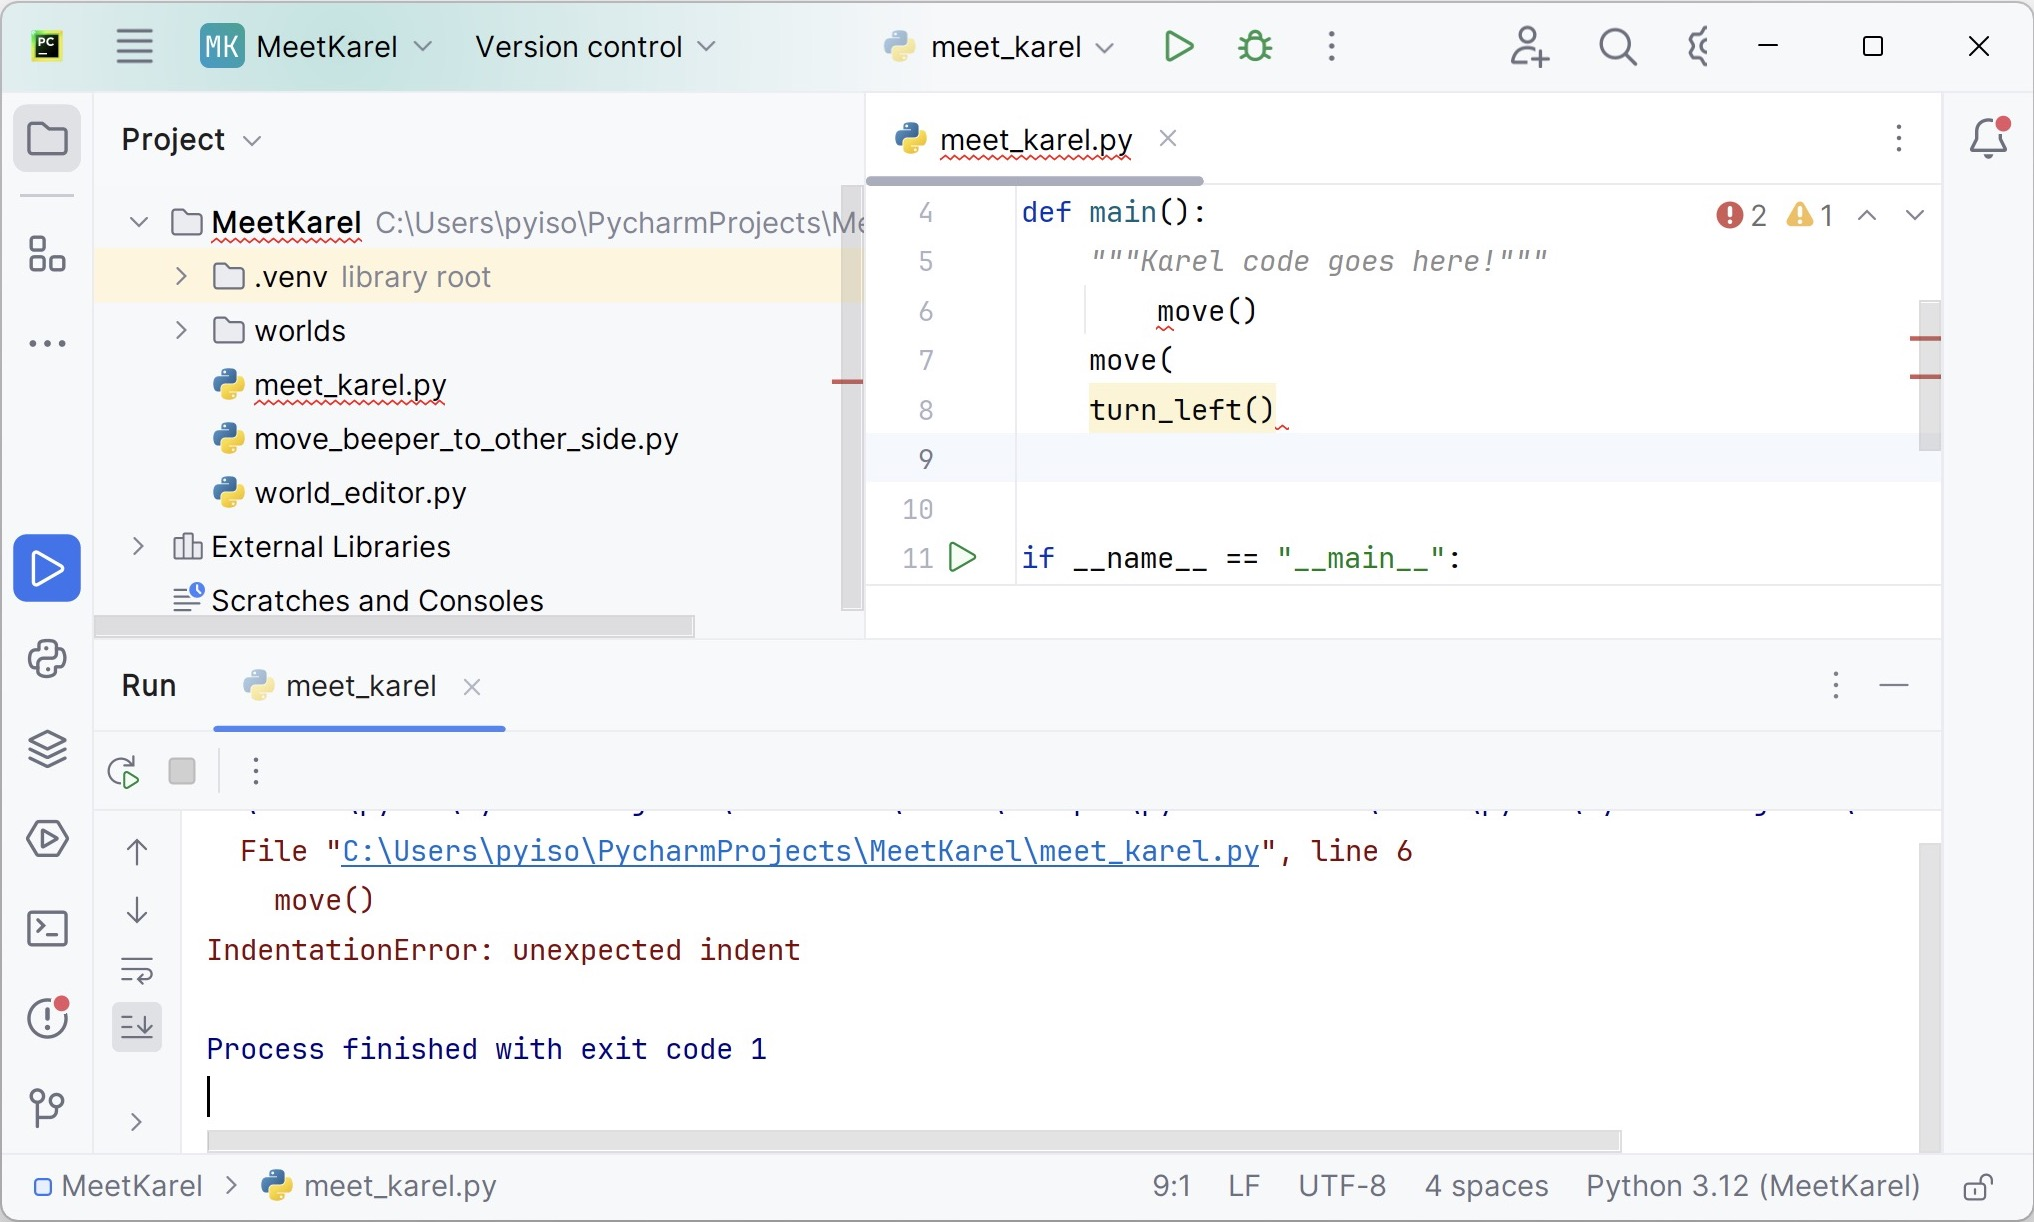
\includegraphics[width=.98\textwidth, trim={2.4mm 2mm 2mm 2mm},clip]{images/pycharm_install/sntxerr.jpg}};
    \drawshadow{image}
\end{tikzpicture}
\caption{} 
\label{fig:sntxerr}
\end{figure}
အကယ်၍ ပရိုဂရမ် \fEn{run} လို့မရရင် ကုဒ်ရေးတာမှားနေလို့ ဖြစ်နိုင်တယ်။ မိမိရေးထားတာကို စာမျက်နှာ (\fRefNo{\pageref{lst:mtkrl}}) က ပရိုဂရမ်ကုဒ်နဲ့  နှိုင်းယှဉ် စစ်ဆေးကြည့်ပါ။ \fEn{PyCharm} အယ်ဒီတာမှာ အနီလှိုင့်တွန့်လေးတွေ (ပုံ \fRefNo{\ref{fig:sntxerr}}) ပြတဲ့နေရင် အဲဒီနေရာတွေမှာ ဆင်းတက်စ်မှားနေလို့ (သို့) လိုက်ဘရီမထည့်ရသေးလို့ပဲ။

ဝိုက်ကွင်းကျန်နေတာက အဖြစ်များတဲ့ အမှားပါ။ ကျန်ခဲ့လို မရပါဘူး။ အင်ဒန့်တေးရှင်း \fEn{(indentation)} လုပ်ရမဲ့နေရာမှာ မလုပ်ထားရင်လည်း ပြဿနာဖြစ်တယ်။ \fCode{move}\fEn{,} \fCode{turn\_left} တွေကို ဘေးမျဉ်းညာဘက်ခွာပြီး အင်ဒန့်လုပ်ပေးရမယ်။ အဲဒါတွေ ဂရုမစိုက်မိရင် ဆင်းတက်စ်အမှားဖြစ်ပြီး ပရိုဂရမ် \fEn{run} လို့ မရနိုင်ဘူး။

\fEnSnd{Terminal} မှာ ထုတ်ပေးတဲ့ \fOpn{မက်ဆေ့ချ်}တွေကို ကြည့်ပြီးတော့လည်း ဘာပြဿနာဖြစ်နေလဲ မှန်းဆလို့ရနိုင်တယ်။ ဘာကြောင့်ဖြစ်နိုင်လဲ ဆက်စပ်စဉ်းစားလို့ ရတယ်။ ဥပမာ ဖြစ်တဲ့ပြဿနာအလိုက် အခုလိုတွေ့ရပါမယ်။ 
%
\begin{minted}[frame=lines, framerule=0pt,escapeinside=ßß]{text}
File "c:\Users\pyiso\VS Code\meet_karel\meet_karel.py", ß\mytcboxinl[yellow]{line 6}ß
    move(
          ^
    ß\mytcboxinl[yellow]{SyntaxError: '(' was never closed}ß
\end{minted}
%
%
\begin{minted}[frame=lines, framerule=0pt,escapeinside=ßß]{text}
File "c:\Users\pyiso\VS Code\meet_karel\meet_karel.py", ß\mytcboxinl[yellow]{line 7}ß
    move()
    ß\mytcboxinl[yellow]{IndentationError: unexpected indent}ß 
\end{minted}
%
%
\begin{minted}[frame=lines, framerule=0pt, escapeinside=ßß]{text}
Traceback (most recent call last):
  File "c:\Users\pyiso\VS Code\meet_karel\meet_karel.py", ß\mytcboxinl[yellow]{line 1}ß, 
        in <module>
    from stanfordkarel import *
    ß\mytcboxinl[yellow]{ModuleNotFoundError: No module named 'stanfordkarel'}ß
\end{minted}
%
\clearpage

\subsection*{Python ဖိုင် အသစ်ယူခြင်း}
\fEnSnd{MeetKarel} ပင်မ ပရောဂျက်ဖိုဒါပေါ်မှာ ညာကလစ်နှိပ်ပြီး \fEn{Python} ဖိုင် အသစ်ယူနိုင်ပါတယ်။ \fEn{Python} ဖိုင်တွေက \fEnSnd{.py} အိပ်စ်တန်းရှင်းနဲ့ပါ။ ကားရဲလ်ပရိုဂရမ်တစ်ခုကို \fEn{Python} ဖိုင်တစ်ခု ထားပါမယ်။ ပင်မ ပရောဂျက်ဖိုဒါ အောက်မှာပဲ တိုက်ရိုက်ရှိရပါမယ်။ 

နောက်ပိုင်း အဆင့်မြင့်လာရင် ပရိုဂရမ်တစ်ခုအတွက် ပရောဂျက်တစ်ခု ထားနိုင်တယ်။ ကုဒ်ဖိုင်တွေအပြင် ပရိုဂရမ်အတွက် လိုအပ်တဲ့ ရုပ်ပုံတွေ၊ အခြားဖိုင်တွေ (\fEn{config} ဖိုင်၊ \fEn{setting} ဖိုင် စသည်ဖြင့်) လည်း ပါနိုင်တယ်။ ပင်မပရောဂျက် အောက်မှာပဲ  ဖိုင်တွေက တိုက်ရိုက်ရှိဖို့လည်း မလိုတော့ဘူး။  ဆက်{\allowbreak}စပ်ရာ ဖိုင်တွေကို အမျိုးအစားအလိုက်၊  ဖန်ရှင်အလိုက် ဖိုဒါတွေခွဲပြီး  စနစ်ကျ စီစဉ်ဖွဲ့စည်း ထားရမှာပါ။ ပရောဂျက်တစ်ခုမှာ ဖိုင်တွေကို စနစ်တကျ စုဖွဲ့ထားဖို့ အရေးကြီးပါတယ်။

\begin{figure}[tbh!]
\begin{tikzpicture}
    \node[anchor=south west,inner sep=0] (image) at (0,0)
        {\includegraphics[width=.98\textwidth, trim={2.4mm 2mm 2mm 2mm},clip]{images/pycharm_install/newfile.jpg}};
    \drawshadow{image}
\end{tikzpicture}
\caption{} 
\label{fig:newfile}
\end{figure}

\clearpage



\section*{Visual Studio Code နှင့် Python အင်စတောလ်လုပ်ခြင်း}
\fEn{Visual Studio Code(VS Code)} ဟာ ပရိုဂရမ်မာအများစု ကြိုက်နှစ်သက်တဲ့ မော်ဒန် ကုဒ်အယ်ဒီတာ တစ်ခုပါ။ \fEn{Python, JavaScript, C++} စတဲ့ \fEn{programming language} အမျိုးမျိုးအတွက် အသုံးပြုနိုင်ပါတယ်။

\fEn{PyCharm} မှာတော့ ပရောဂျက်အသစ်ဆောက်ရင် \fEn{Python} ပါ တစ်ခါတည်း ဒေါင်းလုဒ်လုပ်ပြီး အင်စတောလ် လုပ်လို့ရတယ်။  \fEn{VS Code} နဲ့ \fEn{Python} ရေးမယ်ဆိုရင် \fEn{Python Programming Language} ကို သီးခြား ဒေါင်းလုဒ်လုပ်ပြီး အင်စတောလ် လုပ်ရပါမယ်။ 
\subsection*{Python အင်စတောလ်လုပ်ခြင်း}
ဒီလင့် \fCode{https://www.python.org/} ကိုဖွင့်ပါ။ \fEnSnd{Download} မီနူးမှ \fEnSnd{Windows} နှိပ်ပါ (ပုံ \fRefNo{\ref{fig:pyhome}} ကိုကြည့်ပါ)။ \fEn{Apple} ကွန်ပျူတာအတွက် ဆိုရင် \fEnSnd{macOS} ရွေးရပါမယ်။ လူများစုသုံးတဲ့ မိုက်ခရိုဆော့ဖ် ဝင်းဒိုးအတွက် အင်စတောလ်လုပ်နည်းကို အဓိကပြပေးမှာပါ။ ပုံ \fRefNo{\ref{fig:pyvers}} မှာလို တွေ့ရပါလိမ့်မယ်။ အင်စတော်လာ ဗားရှင်း \fEn{3.12} ထဲက လက်ရှိအမြင့်ဆုံး ကိုရွေးပါ။ ဒီစာရေးချိန်မှာ \fEn{3.12.2} ဟာ အမြင့်ဆုံးဗားရှင်းပါ။ \mytcboxinl{\fEnSnd{Windows Installer (64-bit)}} ကိုနှိပ်ပြီး ဒေါင်းလုဒ်လုပ်ပါ။

\todo{linux အတွက် ဖော်ပြရန်}
\begin{figure}[tbh!]
\begin{tikzpicture}
    \node[anchor=south west,inner sep=0] (image) at (0,0)
        {\includegraphics[width=.98\textwidth, trim={2.4mm 2mm 2mm 2mm},clip]{images/vscode_install/1.jpg}};
    \drawshadow{image}
\end{tikzpicture}
\caption{} 
\label{fig:pyhome}
\end{figure}

\begin{figure}[tbh!]
\begin{tikzpicture}
    \node[anchor=south west,inner sep=0] (image) at (0,0)
        {\includegraphics[width=.98\textwidth, trim={2.4mm 2mm 2mm 2mm},clip]{images/vscode_install/2.jpg}};
    \drawshadow{image}
    \draw [draw=red,very thick,rounded corners] (0.5,7) rectangle (6,7.78);
    \draw [draw=red,very thick,rounded corners] (0.75,4.38) rectangle (4.9,4.8);

\end{tikzpicture}
\caption{} 
\label{fig:pyvers}
\end{figure}

ဒေါင်းလုဒ်ပြီးရင် အင်စတော်လာဖိုင်ကို ညာကလစ်နှိပ်ပြီး \mytcboxinl{\fEnSnd{Run as administrator}} လုပ်ပါ။ ပုံ (\fRefNo{\ref{fig:pyinstlrun}}) ကိုကြည့်ပါ။ ပုံ (\fRefNo{\ref{fig:pyinstl1}}) မှာလို ဒိုင်ယာလော့ဂ် ဘောက်စ် ပွင့်လာပါမယ်။ အနီဝိုင်းထားတဲ့ ချက်ခ်ဘောက်စ်နှစ်ခုကို ချက်ခ်လုပ်ပြီး \mytcboxinl{\fEnSnd{Install Now}} နှိပ်ပါ။ အင်စတောလ် ပြီးလို့ \mytcboxinl{\fEnSnd{Setup was successful}} ပေါ်လာရင် \mytcboxinl{\fEnSnd{Close}} ခလုတ်နှိပ်ပြီး ပိတ်ပါ။

ဝင်းဒိုး \fEnSnd{command prompt (cmd)} မှာ \mytcboxinl{\fCode{python --version}} \fEn{run} ရင် ပုံ (\fRefNo{\ref{fig:pycmdchk}}) မှာလို အင်စတောလ်လုပ်ထားတဲ့ ဗားရှင်းကို ပြပေးသင့်ပါတယ်။
\begin{figure}[tbh!]
\begin{tikzpicture}
    \node[anchor=south west,inner sep=0] (image) at (0,0)
        {\includegraphics[width=.98\textwidth, trim={2.4mm 2mm 2mm 2mm},clip]{images/vscode_install/3.jpg}};
    \drawshadow{image}
\end{tikzpicture}
\caption{} 
\label{fig:pyinstlrun}
\end{figure}

\begin{figure}[tbh!]
\begin{tikzpicture}
    \node[anchor=south west,inner sep=0] (image) at (0,0)
        {\includegraphics[width=.98\textwidth, trim={2.4mm 2mm 2mm 2mm},clip]{images/vscode_install/4.jpg}};
    \drawshadow{image}
    \draw [draw=red,very thick,rounded corners] (3.5,0.24) rectangle (9.25,1.15);
    \draw [draw=red, thick,rounded corners] (3.73,5.1) rectangle (10.75,4.35);
\end{tikzpicture}
\caption{} 
\label{fig:pyinstl1}
\end{figure}

\begin{figure}[tbh!]
\begin{tikzpicture}
    \node[anchor=south west,inner sep=0] (image) at (0,0)
        {\includegraphics[width=.98\textwidth, trim={2.4mm 2mm 2mm 2mm},clip]{images/vscode_install/5.jpg}};
    \drawshadow{image}
\end{tikzpicture}
\caption{} 
\label{fig:pycmdchk}
\end{figure}

\clearpage
\subsection*{VS Code အင်စတောလ်လုပ်ခြင်း}\label{sec:vscode}
အခုဆိုရင် \fEn{Python programming language} အောင်မြင်စွာ ထည့်ပြီးသွားပါပြီ။ \fEn{VS Code} အင်စတောလ် ဆက်လုပ်ပါမယ်။ အင်စတာ်လာ ဒေါင်းလုဒ်လုပ်ရန် ဝဘ်စာမျက်နှာကို အောက်ပါလင့်
%
\begin{minted}[frame=lines, framerule=0pt]{text}
https://code.visualstudio.com 
\end{minted}
%
မှတစ်ဆင့် သွားပါ။ ပုံ (\fRefNo{\ref{fig:vsdwnpg}}) ဝဘ်စာမျက်နှာကို တွေ့ရပါမယ်။ \mytcboxinl{\fEnSnd{Download for Windows}} နှိပ်၍ ဒေါင်းလုဒ်လုပ်ပါ။

ပြီးတဲ့အခါ အင်စတော်လာဖိုင်ကို ညာကလစ်နှိပ်ပြီး ဖွင့်ပါ (ပုံ \fRefNo{\ref{fig:vsinstlropn}} မှာ ပြထားပါတယ်)။ အင်စတောလ် ဒိုင်ယာလော့ဂ်ဘောက်စ် ပွင့်လာရင် \mytcboxinl{\fEnSnd{I accept the agreement}} ကို ချက်ခ်လုပ်၍ \fEnSnd{Next>} တစ်ခုပြီးတစ်ခု ဆက်နှိပ်သွားပြီး နောက်ဆုံးမှာ  \fEnSnd{Install} နှိပ်ပါ။ အင်စတောလ်လုပ်နေတာကို ခဏစောင့်ပြီး၊ ပြီးသွားရင် \fEnSnd{Finish} နှိပ်ပါ။  

\fEn{Welcome} စခရင်ကို ပုံ (\fRefNo{\ref{fig:vswlcm}}) လို တွေ့ရပါမယ်။ \mytcboxinl{\fEnSnd{Dark Modern}} (သို့) \mytcboxinl{\fEnSnd{Light Modern}} နှစ်သက်ရာ သီးမ်စ် ရွေးပါ။ ဒါဆိုရင် \fEn{VS Code} လည်း အင်စတောလ် လုပ်ပြီးသွားပါပြီ။ ကားရဲလ်ပရိုဂရမ် ရေးဖို့ ဆက်လုပ်ရပါမယ်။

\begin{figure}[tbh!]
\begin{tikzpicture}
    \node[anchor=south west,inner sep=0] (image) at (0,0)
        {\includegraphics[width=.98\textwidth, trim={2.4mm 2cm 2mm 2mm},clip]{images/vscode_install/v0.jpg}};
    \drawshadow{image}
\end{tikzpicture}
\caption{} 
\label{fig:vsdwnpg}
\end{figure}

\begin{figure}[tbh!]
\begin{tikzpicture}
    \node[anchor=south west,inner sep=0] (image) at (0,0)
        {\includegraphics[width=.98\textwidth, trim={2.4mm 2mm 2mm 2mm},clip]{images/vscode_install/v1.jpg}};
    \drawshadow{image}
\end{tikzpicture}
\caption{} 
\label{fig:vsinstlropn}
\end{figure}

\begin{figure}[tbh!]
\begin{tikzpicture}
    \node[anchor=south west,inner sep=0] (image) at (0,0)
        {\includegraphics[width=.98\textwidth, trim={2.4mm 2mm 2mm 2mm},clip]{images/vscode_install/v1b.jpg}};
    \drawshadow{image}
    
    \draw [draw=red,very thick,rounded corners] (6.25,7.5) rectangle (9.08,5.25);
    \draw [draw=red,very thick,rounded corners] (9.35,7.5) rectangle (12.01,5.25);
    \draw [draw=red,very thick,rounded corners] (0.08,5.5) rectangle (0.6,5);
\end{tikzpicture}
\caption{} 
\label{fig:vswlcm}
\end{figure}

\clearpage

\subsection*{VS Code Python Extension ထည့်ခြင်း}
\fEn{Python} ပရိုဂရမ်ရေးဖို့အတွက် \fEn{VS Code} က ဒီအတိုင်းဆိုရင် သိပ်အဆင်မပြေသေးပါဘူး။ \fEn{Python} အတွက် \fEn{extension} အင်စတောလ် လုပ်ပေးရပါအုံးမယ်။ ပုံ (\fRefNo{\ref{fig:vswlcm}}) ဘယ်ဘက်ဘောင်နားမှာ အနီဝိုင်းထားတဲ့ အိုင်ကွန်လေးကို နှိပ်ပါ။ \fEn{Python} \fEnSnd{extension} ကိုရှာပါ။   ပုံ (\fRefNo{\ref{fig:vspyplugin1}}) မှာ ဘယ်လိုရှာရမလဲ ပြထားပါတယ်။ ပုံမှာတွေ့ရတဲ့ \fEn{Microsoft} က ထုတ်တဲ့ \fEnSnd{extension} ကို အင်စတောလ်လုပ်ပါ။ အောင်မြင်ရင် ပုံ (\fRefNo{\ref{fig:vspyplugin2}}) မှာလို ဖြစ်သွားပါမယ်။ \fEn{Python} နဲ့  \fEn{VS Code} ကိစ္စတော့ ပြီးသွားပြီ။ ကားရဲလ် \fEn{example} \fEn{run} ဖို့ ဆက်လုပ်ရမယ်။
\begin{figure}[tbh!]
\begin{tikzpicture}
    \node[anchor=south west,inner sep=0] (image) at (0,0)
        {\includegraphics[width=.98\textwidth, trim={2.4mm 2mm 2mm 2mm},clip]{images/vscode_install/v2.jpg}};
    \drawshadow{image}
\end{tikzpicture}
\caption{} 
\label{fig:vspyplugin1}
\end{figure}

\begin{figure}[tbh!]
\begin{tikzpicture}
    \node[anchor=south west,inner sep=0] (image) at (0,0)
        {\includegraphics[width=.98\textwidth, trim={2.4mm 2mm 2mm 2mm},clip]{images/vscode_install/v3.jpg}};
    \drawshadow{image}
\end{tikzpicture}
\caption{} 
\label{fig:vspyplugin2}
\end{figure}

\clearpage

\subsection*{နမူနာ ကားရဲလ် ကမ္ဘာနှင့် ပရိုဂရမ်ကုဒ် ဖိုင်များထည့်ခြင်း}
\fEnSnd{meet\_karel.zip} ဖိုင်ကို \todo{ဒေါင်းလုဒ်လင့်ထည့်ရန်} ဒီလင့် \fCode{http://tinyurl.com/3mmm9c7j} ကနေ ဒေါင်းလုဒ်လုပ်ပါ။ ၎င်း \fEnSnd{zip} ဖိုင်ကို \fEn{extract} လုပ်ပါ။ \fEnSnd{meet\_karel} နံမည်နဲ့ ဖိုဒါတစ်ခု ရလာပါမယ်။ ဖိုဒါထဲ ဝင်ကြည့်ရင် အောက်ပါအတိုင်း ရှိသင့်ပါတယ်။ 
%
\begin{itemize}
    \item \fEnSnd{worlds} 
    \begin{itemize}
        \item \fEnSnd{meet\_karel.w}
        \item \fEnSnd{move\_beeper\_to\_other\_side.w}
    \end{itemize}
    \item \fEnSnd{meet\_karel.py}
    \item \fEnSnd{move\_beeper\_to\_other\_side.py}
    \item \fEnSnd{world\_editor.py}
\end{itemize}
%

\begin{figure}[tbh!]
\begin{tikzpicture}
    \node[anchor=south west,inner sep=0] (image) at (0,0)
        {\includegraphics[width=.98\textwidth, trim={2.4mm 2mm 2mm 2mm},clip]{images/vscode_install/v4.jpg}};
    \drawshadow{image}
\end{tikzpicture}
\caption{} 
\label{fig:mtkrl1}
\end{figure}

\begin{figure}[tbh!]
\begin{tikzpicture}
    \node[anchor=south west,inner sep=0] (image) at (0,0)
        {\includegraphics[width=.98\textwidth, trim={2.4mm 2mm 2mm 2mm},clip]{images/vscode_install/v5b.jpg}};
    \drawshadow{image}
\end{tikzpicture}
\caption{} 
\label{fig:opnmtkrl}
\end{figure}

\begin{figure}[tbh!]
\begin{tikzpicture}
    \node[anchor=south west,inner sep=0] (image) at (0,0)
        {\includegraphics[width=.98\textwidth, trim={2.4mm 2mm 2mm 2mm},clip]{images/vscode_install/v6.jpg}};
    \drawshadow{image}
\end{tikzpicture}
\caption{} 
\label{fig:mtkrl3}
\end{figure}

\fEn{VS Code} အတွက် ဖိုဒါတစ်ခုကို မိမိအတွက် အဆင်ပြေမဲ့နေရာမှာ သီးသန့်တည်ဆောက် ထားသင့်တယ်။ ဥပမာ 
%
\begin{minted}[frame=lines, framerule=0pt,escapeinside=ßß]{text}
ß\fEnSnd{C:{\textbackslash}Users{\textbackslash}\textit{yourname}{\textbackslash}VS Code}ß
\end{minted}
%
\begin{mytcbox}
မိမိ လက်ရှိ \fEn{Home} ဖိုဒါကို  \mytcboxinl{\fEnSnd{C:}} \fEn{drive} ရဲ့ \mytcboxinl{\fEnSnd{Users}}  ဖိုဒါထဲမှာ တွေ့နိုင်ပါတယ်။ \mytcboxinl{\fEnSnd{Win + R}} ရှော့ကတ်နှိပ်ပြီး \mintinline{text}|%userprofile%| ရိုက်ထည့်၊ \fEnSnd{Ok} လုပ်ပြီး \fEn{Home} ဖိုဒါကို သွားနိုင်ပါတယ်။ အကယ်၍ မသွားတတ်ရင်လည်း ပြဿနာမရှိပါဘူး။ ကိုယ့်အတွက် လွယ်ကူမဲ့ \fEnSnd{Desktop, Downloads, Documents} တစ်ခုခုထဲမှာ \fEn{VS Code} အတွက် ဖိုဒါတစ်ခု ထားလည်းရတယ်။
\end{mytcbox}

\mytcboxinl{\fEnSnd{meet\_karel}} ဖိုဒါ (\fEnSnd{.zip} ဖိုင်မဟုတ်ပါ) ကို အထက်ပါအတိုင်း အသစ် ဆောက်ထားတဲ့ \fEn{VS Code} သီးသန့်ဖိုဒါထဲကို ကော်ပီကူးထည့်ပါ။ ၎င်း \mytcboxinl{\fEnSnd{meet\_karel}} ဖိုဒါကို \fEn{VS Code} \mytcboxinl{\fEnSnd{File}} မီနူးမှ \mytcboxinl{\fEnSnd{Open Folder}} နှိပ်၍ ဖွင့်ပါ။ ပုံ (\fRefNo{\ref{fig:opnmtkrl}}) တွင်ကြည့်ပါ။

အခန်းအလိုက် နမူနာ ကုဒ်ဖိုင်တွေ ထည့်ပေးထားတဲ့ \fEnSnd{.zip} ဖိုင်တွေကိုလည်း အထက်ပါအတိုင်း လုပ်ရပါမယ်။ \fEnSnd{.zip} ဖိုင်ကို ဖြည်၊ ရလာတဲ့ ဖိုဒါကို သီးသန့်ဖိုဒါတစ်ခုထဲကို ကော်ပီကူးထည့်၊ \fEn{VS Code} နဲ့ အဲ့ဒီဖိုဒါကို ဖွင့်ရုံပါပဲ။



\clearpage
\subsection*{stanfordkarel လိုက်ဘရီ အင်စတောလ်လုပ်ခြင်း}
\mytcboxinl{\fEnSnd{meet\_karel.py}} ဖိုင်ကို ကလစ်နှစ်ချက်နှိပ် ဖွင့်ပါ။ ကုဒ်အယ်ဒီတာ ပွင့်လာမယ် (ပုံ \fRefNo{\ref{fig:edtmtkrl}})။ အဲဒီ ကုဒ်အယ်ဒီတာပေါ် (သို့) \mytcboxinl{\fEnSnd{meet\_karel.py}} ဖိုင်ကို ညာကလစ်နှိပ်ပြီး \mytcboxinl{\fEnSnd{Run Python File in Terminal}} လုပ်ပါ (ပုံ \fRefNo{\ref{fig:runmtkrl2}})။ \fEnSnd{Terminal} ပွင့်လာပြီး အယ်ရာ\fOpn{မက်ဆေ့ချ်}တွေ ပြလိမ့်မယ်။ ပုံ (\fRefNo{\ref{fig:mtkrlfstrun}}) မှာကြည့်ပါ။ ကားရဲလ်ပရိုဂရမ်အတွက် လိုအပ်တဲ့ \fEnSnd{stanfordkarel} လိုက်ဘရီ အင်စတောလ် မလုပ်ရသေးပါဘူး။ ဒါကြောင့် အယ်ရာဖြစ်နေတာ။

\begin{figure}[tbh!]
\begin{tikzpicture}
    \node[anchor=south west,inner sep=0] (image) at (0,0)
        {\includegraphics[width=.98\textwidth, trim={2.4mm 2mm 2mm 2mm},clip]{images/vscode_install/v7.jpg}};
    \drawshadow{image}
\end{tikzpicture}
\caption{} 
\label{fig:edtmtkrl}
\end{figure}

\begin{figure}[tbh!]
\begin{tikzpicture}
    \node[anchor=south west,inner sep=0] (image) at (0,0)
        {\includegraphics[width=.98\textwidth, trim={2.4mm 2mm 2mm 2mm},clip]{images/vscode_install/v9.jpg}};
    \drawshadow{image}
\end{tikzpicture}
\caption{} 
\label{fig:runmtkrl2}
\end{figure}

\begin{figure}[tbh!]
\begin{tikzpicture}
    \node[anchor=south west,inner sep=0] (image) at (0,0)
        {\includegraphics[width=.98\textwidth, trim={2.4mm 2mm 2mm 2mm},clip]{images/vscode_install/v8.jpg}};
    \drawshadow{image}
\end{tikzpicture}
\caption{} 
\label{fig:mtkrlfstrun}
\end{figure}
ခုနကပွင့်လာတဲ့ \fEnSnd{Terminal} မှာပဲ အောက်ပါကွန်မန်းကို \fEn{run} ပြီး \fEnSnd{stanfordkarel} လိုက်ဘရီကို အင်စတောလ်လုပ်ပါ။ 
%
\begin{minted}[frame=lines, framerule=0pt]{text}
pip install stanfordkarel
\end{minted}
%
ပုံ (\fRefNo{\ref{fig:mtkrlfstrun}}) မှာ အနီဝိုင်းထားတာကို ကြည့်ပါ။ အဲဒီအတိုင်းရိုက်ထည့်ပြီး \fEnSnd{Enter} ကီးနှိပ်ပါ။ ခဏကြာတဲ့အခါ အခုလို \fOpn{မက်ဆေ့ချ်}တွေ ကျလာပါလိမ့်မယ်။ 

%
\begin{minted}[frame=lines, framerule=0pt,escapeinside=ßß]{text}
ModuleNotFoundError: No module named 'stanfordkarel'
PS C:\Users\pyiso\VSCode\meet_karel> pip install stanfordkarel
Collecting stanfordkarel
  Downloading stanfordkarel-0.2.7-py3-none-any.whl (51 kB)
     ━━━━━━━━━━━━━━━━━━━━━━━ 51.9/51.9 kB 295.4 kB/s eta 0:00:00
Installing collected packages: stanfordkarel
ß\mytcboxinl[yellow]{Successfully installed stanfordkarel-0.2.7}ß
PS C:\Users\pyiso\VSCode\meet_karel> 
\end{minted}
%
ဟိုက်လိုက်ပြထားတဲ့ \fOpn{မက်ဆေ့ချ်} တွေ့ရရင် အင်စတောလ် အောင်မြင်လို့ပါ။ ပုံ (\fRefNo{\ref{fig:edtmtkrl}}) အယ်ဒီတာမှာလို သတိပေး လှိုင်းတွန့်မျဉ်းတွေ မရှိသင့်တော့ဘူး။ \fEnSnd{stanfordkarel} လိုက်ဘရီ အင်စတောလ် လုပ်ပြီးပြီမိုလို့ သတိပေးတာတွေ ပျောက်သွားသင့်တယ်။


\mytcboxinl{\fEnSnd{meet\_karel.py}} ဖိုင်ကို ညာကလစ်နှိပ်ပြီး \mytcboxinl{\fEnSnd{Run Python File in Terminal}} ပြန်လုပ်ကြည့်ပါ။ ပုံ (\fRefNo{\ref{fig:mtkrlprgm}}) မှာပြထားတဲ့ ကားရဲလ်ပရိုဂရမ် ပွင့်လာသင့်ပါတယ်။ \mytcboxinl{\fEnSnd{Run Program}} နှိပ်ကြည့်ပါ။ စက်ရုပ်လေး ကားရဲလ် နေရာရွေ့သွားတာ တွေ့ရမယ်။ \mytcboxinl{\fEnSnd{meet\_karel.py}} ကို အောက်ပါအတိုင်း ဖြည့်စွက်ရေးပါ။
\begin{figure}[tbh!]
\begin{tikzpicture}
    \node[anchor=south west,inner sep=0] (image) at (0,0)
        {\includegraphics[width=.98\textwidth, trim={2.4mm 2mm 2mm 2mm},clip]{images/vscode_install/mtkrlprgm.jpg}};
    \drawshadow{image}
\end{tikzpicture}
\caption{} 
\label{fig:mtkrlprgm}
\end{figure}


%
\setlength{\fboxsep}{0pt}
\begin{minted}[frame=\mintframe, framerule=\mintrule,framesep= \mintsep, xleftmargin=\xlftmargin
                , bgcolor=mintbgcolor,rulecolor=mintrulecolor
                , python3=true]{python}
from stanfordkarel import *


def main():
    """Karel code goes here!"""
    move()
    move()
    move()
    pick_beeper()
    turn_left()
    move()
    move()

    turn_left()
    turn_left()
    turn_left()

    move()
    put_beeper()


if __name__ == "__main__":
    run_karel_program("meet_karel")
\end{minted}
%

\mytcboxinl{\fEnSnd{meet\_karel.py}} ဖိုင်ကို ညာကလစ်နှိပ်ပြီး \mytcboxinl{\fEnSnd{Run Python File in Terminal}} ပြန်လုပ်ကြည့်ပါ။ ကားရဲလ်ပရိုဂရမ် ပွင့်လာရင် \mytcboxinl{\fEnSnd{Run Program}} နှိပ်ကြည့်ပါ။ ဘိပါလေးကို နေရာရွှေ့ပေးပါလိမ့်မယ်။ အကယ်၍ ကားရဲလ်ပရိုဂရမ် မတက်လာရင် ကုဒ်ရေးတာမှားနေလို့ ဖြစ်နိုင်တယ်။ အပေါ်ကုဒ်နဲ့ နှိုင်းယှဉ်ပြီး ကြည့်ပါ။ \fEn{VS Code} အယ်ဒီတာမှာ အနီလှိုင့်တွန့်လေးတွေ ပြတဲ့နေရင် အဲဒီနေရာတွေမှာ ဆင်းတက်စ်မှားနေတာ ဖြစ်နိုင်တယ်။
%
\begin{mytcbox}
\fEn{VS Code} အယ်ဒီတာမှာ ပရိုဂရမ်ကုဒ်ပြင်ပြီး ပြန် \fEn{run} တဲ့အခါ ပထမ \fEn{run} ထားတဲ့ ပရိုဂရမ်ကို အရင်ပိတ်ဖို့လိုပါတယ်။ ဆိုလိုတာက \fEnSnd{meet\_karel.py} ကို \fEn{run} ထားတယ်ဆိုပါစို့။ ပုံ (\fRefNo{\ref{fig:mtkrlprgm}}) က ဝင်းဒိုးပွင့်လာမယ်။ \fEnSnd{meet\_karel.py} ကုဒ်ကို ပြင်ပြီး ပြန် \fEn{run} ချင်ရင် အဲဒီ ဝင်းဒိုးကို အရင်ပိတ်ရမယ်။ မဟုတ်ရင် ပြင်ထားတဲ့ ပရိုဂရမ်က ချက်ချင်း ပွင့်မလာဘူး။ ပထမ ဟာကို ပိတ်တော့မှပဲ နောက် \fEn{run} တဲ့ဟာ ပွင့်လာမှာ။ 
\end{mytcbox}
%
ဝိုက်ကွင်းကျန်နေတာက အဖြစ်များတဲ့ အမှားပါ။ ကျန်ခဲ့လို မရပါဘူး။ အင်ဒန့်တေးရှင်း \fEn{(indentation)} လုပ်ရမဲ့နေရာမှာ မလုပ်ထားရင်လည်း ပြဿနာဖြစ်တယ်။ \fCode{move}\fEn{,} \fCode{turn\_left} တွေကို ဘေးမျဉ်းညာဘက်ခွာပြီး အင်ဒန့်လုပ်ပေးရမယ်။ အဲဒါတွေ ဂရုမစိုက်မိရင် ဆင်းတက်စ်အမှားဖြစ်ပြီး ပရိုဂရမ် \fEn{run} လို့ မရနိုင်ဘူး။

\fEnSnd{Terminal} မှာ ထုတ်ပေးတဲ့ \fOpn{မက်ဆေ့ချ်}တွေကို ကြည့်ပြီးတော့လည်း ဘာပြဿနာဖြစ်နေလဲ မှန်းဆလို့ရနိုင်တယ်။ ဘာကြောင့်ဖြစ်နိုင်လဲ ဆက်စပ်စဉ်းစားလို့ ရတယ်။ ဥပမာ ဖြစ်တဲ့ပြဿနာအလိုက် အခုလိုတွေ့ရပါမယ်။ 
%
\begin{minted}[frame=lines, framerule=0pt,escapeinside=ßß]{text}
File "c:\Users\pyiso\VS Code\meet_karel\meet_karel.py", ß\mytcboxinl[yellow]{line 6}ß
    move(
          ^
    ß\mytcboxinl[yellow]{SyntaxError: '(' was never closed}ß
\end{minted}
%
%
\begin{minted}[frame=lines, framerule=0pt,escapeinside=ßß]{text}
File "c:\Users\pyiso\VS Code\meet_karel\meet_karel.py", ß\mytcboxinl[yellow]{line 7}ß
    move()
    ß\mytcboxinl[yellow]{IndentationError: unexpected indent}ß 
\end{minted}
%
%
\begin{minted}[frame=lines, framerule=0pt, escapeinside=ßß]{text}
Traceback (most recent call last):
  File "c:\Users\pyiso\VS Code\meet_karel\meet_karel.py", ß\mytcboxinl[yellow]{line 1}ß, 
        in <module>
    from stanfordkarel import *
    ß\mytcboxinl[yellow]{ModuleNotFoundError: No module named 'stanfordkarel'}ß
\end{minted}
%



\clearpage


\subsection*{VS Code တွင် Python ဖိုင် အသစ်ယူခြင်း}
\fEnSnd{MEET\_KAREL} ပင်မ ပရောဂျက်ဖိုဒါပေါ်မှာ ကလစ်နှိပ်ပါ။ ပုံမှာ ပြထားတဲ့ \mytcboxinl{\fEnSnd{New File}} အိုင်ကွန်ကိုနှိပ်ပါ။ ဖိုင်နံမည်ဖြည့်တဲ့ ဘောက်စ်လေး ပေါ်လာမယ်။ \fEn{Python} ဖိုင်တွေက \fEnSnd{.py} အိပ်စ်တန်းရှင်းနဲ့ ဖြစ်ရပါမယ်။ ဒါကြောင့် နံမည် ဖြည့်တဲ့အခါ \fEnSnd{.py} နဲ့ အဆုံးသတ်ပေးရပါမယ် (ဥပမာ \fEnSnd{hello.py})။ ကားရဲလ်ပရိုဂရမ်တစ်ခုကို \fEn{Python} ဖိုင်တစ်ခု ထားပါမယ်။ ပင်မ ပရောဂျက်ဖိုဒါ အောက်မှာပဲ တိုက်ရိုက်ရှိရပါမယ်။ 

နောက်ပိုင်း အဆင့်မြင့်လာရင် ပရိုဂရမ်တစ်ခုအတွက် ပရောဂျက်တစ်ခု ထားနိုင်တယ်။ ကုဒ်ဖိုင်တွေအပြင် ပရိုဂရမ်အတွက် လိုအပ်တဲ့ ရုပ်ပုံတွေ၊ အခြားဖိုင်တွေ (\fEn{config} ဖိုင်၊ \fEn{setting} ဖိုင် စသည်ဖြင့်) လည်း ပါနိုင်တယ်။ ပင်မပရောဂျက် အောက်မှာပဲ  ဖိုင်တွေက တိုက်ရိုက်ရှိဖို့လည်း မလိုတော့ဘူး။  ဆက်{\allowbreak}စပ်ရာ ဖိုင်တွေကို အမျိုးအစားအလိုက်၊  ဖန်ရှင်အလိုက် ဖိုဒါတွေခွဲပြီး  စနစ်ကျ စီစဉ်ဖွဲ့စည်း ထားရမှာပါ။ ပရောဂျက်တစ်ခုမှာ ဖိုင်တွေကို စနစ်တကျ စုဖွဲ့ထားဖို့ အရေးကြီးပါတယ်။

\begin{figure}[tbh!]
\begin{tikzpicture}
    \node[anchor=south west,inner sep=0] (image) at (0,0)
        {\includegraphics[width=.98\textwidth, trim={2.4mm 2mm 2mm 2mm},clip]{images/vscode_install/newfile.jpg}};
    \drawshadow{image}
\end{tikzpicture}
\caption{} 
\label{fig:vsnewfile}
\end{figure}

\clearpage








\afterpage{\blankpage}

\renewcommand\thefigure{B/\arabic{figure}} 
\chapter{ကားရဲလ်ပရိုဂရမ် ဖီချာများ}\label{apdx:02}

\section*{ကားရဲလ် ကမ္ဘာဖိုင်များ}

ကားရဲလ်ပရိုဂရမ် ဝင်းဒိုးမှာ \mytcboxinl{\fEnSnd{Load World}} ခလုတ်နှိပ်ပြီး ကမ္ဘာဖိုင်အသစ် တင်လို့ရတယ်။ ခလုတ်နှိပ်လိုက်ရင် အခုလို ဖိုင် ဒိုင်ယာလော့ဂ် ပွင့်လာမယ်။

\begin{figure}[tbh!]
\begin{tikzpicture}
    \node[anchor=south west,inner sep=0] (image) at (0,0)
        {\includegraphics[width=.98\textwidth, trim={2mm 2mm 28cm 2.5mm},clip]{images/apdx02/dftworlds.jpg}};
    \drawshadow{image}
\end{tikzpicture}
\caption{} 
\label{fig:dftworlds}
\end{figure}

ဒါက \fEnSnd{stanfordkarel} လိုက်ဘရီ သူ့နဂိုအရှိအတိုင်း ပါတဲ့ \fEnSnd{worlds} ဖိုဒါပါ။ ဖိုင်တွေက  \mytcboxinl{\fEnSnd{.w}} နဲ့ ဆုံးပါတယ်။  ကမ္ဘာဖိုင်တွေကို ပင်မ ပရောဂျက်အောက် \fEnSnd{worlds} ဖိုဒါထဲမှာ ထားလို့လည်းရတယ်။ အခြားနေရာတွေမှာ ထားလို့တော့ မရဘူး။

စာအုပ်ပါ ဥပမာတွေ၊ လေ့ကျင့်ခန်းတွေအတွက် ကမ္ဘာဖိုင်တွေကို ပရောဂျက် တစ်ခုချင်းအလိုက် သီးခြား \fEnSnd{worlds} ဖိုဒါထဲမှာ ထည့်ပေးထားမှာပါ။ ပရိုဂရမ်တစ်ခုဟာ ကမ္ဘာတစ်ခုတည်းမှာပဲ အလုပ်လုပ်တာမဟုတ်ဘဲ အလားတူ ကမ္ဘာအမျိုးမျိုးအတွက် အလုပ်လုပ်အောင် ရေးပေးရတာ။ အခုပြောတာကို နားမလည်ရင် အခန်း (\fRefNo{\ref{ch:ch02}}) ဖတ်ပြီးရင် နားလည်သွားမှာပါ။

\mytcboxinl{\fEnSnd{Load World}} လုပ်တဲ့အခါ ပွင့်လာတဲ့ ဖိုင် ဒိုင်ယာလော့ဂ်က ကိုယ်လိုချင်တဲ့ \fEnSnd{worlds} ဖိုဒါ မဖြစ်နေဘူး။ သူ့နဂိုပါတဲ့ \fEnSnd{worlds} ဖိုဒါ ဖြစ်နေတယ်။ ကိုယ်ခေါ်တင်ချင်တဲ့ ဖိုင်တွေရှိတဲ့ လက်ရှိပရောဂျက်ရဲ့ \fEnSnd{worlds} ဖိုဒါကို သွားရမယ်။ ဥပမာ \fEn{PyCharm/VS Code} အတွက် \fEnSnd{MeetKarel/meet\_karel} ပရောဂျက် \fEnSnd{worlds} ဖိုဒါ လမ်းကြောင်း အပြည့်အစုံက
%
\begin{minted}[frame=lines, framerule=0pt,escapeinside=ßß]{text}
ß\fEnSnd{C:{\textbackslash}Users{\textbackslash}\textit{yourname}{\textbackslash}VSCode{\textbackslash}meet\_karel{\textbackslash}worlds}ß
ß\fEnSnd{C:{\textbackslash}Users{\textbackslash}\textit{yourname}{\textbackslash}PycharmProjects{\textbackslash}MeetKarel{\textbackslash}worlds}ß
\end{minted}
%
ဖြစ်ပါမယ်။ ဖိုင်ဒိုင်ယာလေ့ဂ်ကနေ ဖော်ပြပါ လက်ရှိပရောဂျက် \fEnSnd{worlds} ဖိုဒါကို တစ်ဆင့်ချင်း သွားပြီး တင်ချင်တဲ့ ကမ္ဘာဖိုင် (\fEnSnd{.w} ဖိုင်) ကို ရွေးရမှာပါ။

အပေါ်ကနည်းနဲ့ အဆင်မပြေခဲ့ရင် အခုလိုစမ်းကြည့်ပါ။ လက်ရှိပရောဂျက် \fEnSnd{worlds} ဖိုဒါကို ညာကလစ်နှိပ်ပြီး \fEnSnd{Copy Path} လုပ်ပါ (ပုံ \fRefNo{\ref{fig:cpwldfld}}) ။ ဖိုင် ဒိုင်ယာလော့ဂ် \mytcboxinl{\fEnSnd{File name}} မှာ ကူးထည့်ပါ (ပုံ \fRefNo{\ref{fig:pstepth}})။ \mytcboxinl{\fEnSnd{Enter}} ကီးနှိပ်ပါ။ ပရောဂျက် \fEnSnd{worlds} ဖိုဒါကိုရောက်သွားပါမယ်။ လိုတဲ့ကမ္ဘာဖိုင် ရွေးတင်ရုံပါပဲ။ ပုံ (\fRefNo{\ref{fig:prjwlds}}) မှာ \fEnSnd{meet\_karel} \fEnSnd{worlds} ကို နမူနာပြထားပါတယ်။

\begin{figure}[tbh!]
\begin{tikzpicture}
    \node[anchor=south west,inner sep=0] (image) at (0,0)
        {\includegraphics[width=.98\textwidth, trim={2.4mm 2mm 2mm 2mm},clip]{images/apdx02/cpwldfld.jpg}};
    \drawshadow{image}
\end{tikzpicture}
\caption{} 
\label{fig:cpwldfld}
\end{figure}

\begin{mytcbox}
အကယ်၍ အထက်ဖော်ပြပါနည်းတွေက ရှုပ်နေတယ်ထင်ရင်  မှတ်ရ/သွားရ လွယ်တဲ့ \fEnSnd{Desktop, Downloads, Documents} လို နေရာတစ်ခုခုမှာ  သီးသန့်ဖိုဒါတစ်ခု ဆောက်ပြီး ပရောဂျက်အားလုံး ထည့်ထားတာ အရှင်းဆုံးပါပဲ။ ပရောဂျက်ဖိုဒါနေရာ သိရင် ဖိုင်ဒိုင်ယာလော့ဂ်ကနေ ဘယ်လိုမဆို ရောက်အောင် သွားလို့ရပါတယ်။
\end{mytcbox}

\begin{figure}[tbh!]
\begin{tikzpicture}
    \node[anchor=south west,inner sep=0] (image) at (0,0)
        {\includegraphics[width=.98\textwidth, trim={2.4mm 2mm 28cm 2mm},clip]{images/apdx02/pstepth.jpg}};
    \drawshadow{image}
\end{tikzpicture}
\caption{} 
\label{fig:pstepth}
\end{figure}

\begin{figure}[tbh!]
\begin{tikzpicture}
    \node[anchor=south west,inner sep=0] (image) at (0,0)
        {\includegraphics[width=.98\textwidth, trim={2.4mm 2mm 28cm 2mm},clip]{images/apdx02/prjwlds.jpg}};
    \drawshadow{image}
\end{tikzpicture}
\caption{} 
\label{fig:prjwlds}
\end{figure}


\clearpage

\section*{ကိုယ်ပိုင် ကားရဲလ်ကမ္ဘာ ဆောက်ခြင်း }
ကားရဲလ်ရဲ့ ကမ္ဘာ အသစ်တစ်ခုဆောက်မယ်ဆိုရင် \fEnSnd{world\_editor.py} ဖိုင်ကို ညာကလစ်နှိပ်  \fEnSnd{\mytcboxinl{Run}} ပါ။ \mytcboxinl{\fEnSnd{Would you like to load an existing world?}} လို့ ပေါ်လာပြီး \fEnSnd{Yes/No} ရွေးခိုင်ပါလိမ့်မယ်။ \fEnSnd{No} ကို နှိပ်ပါ။ ကမ္ဘာအရွယ်အစားအတွက် ကော်လံ ဘယ်နှစ်ခုလဲ၊ \fEn{row} ဘယ်နှစ်ခုလဲ ထည့်ပေးပါ။  ကိုယ်ပိုင် ကားရဲလ်ကမ္ဘာ တည်ဆောက်လို့ရတဲ့ ဝင်းဒိုးပွင့်လာပါလိမ့်မယ်။ ကားရဲလ် မျက်နှာမူရာအရပ်၊ ဘိပါအိတ်ထဲရှိ ဘိပါအရေအတွက်၊ နံရံဆောက်/ဖျက်တာ၊ ဘိပါထည့်/ဖယ်ထုတ်တာ စတာတွေ လုပ်နိုင်ပါတယ်။  \mytcboxinl{\fEnSnd{Save World}} နှိပ်ပြီး သိမ်းနိုင်ပါတယ်။ ဖိုင်ကိုသိမ်းတဲ့အခါ သူ့နဂို သိမ်းခိုင်းတဲ့ဖိုဒါ \fEn{(default world folder)} ထဲမှာ သို့မဟုတ် ပင်မ ပရောဂျက်ဖိုဒါထဲက \fEnSnd{worlds} ဖိုဒါထဲမှာ သိမ်းရပါမယ်။  

\begin{figure}[tbh!]
\begin{tikzpicture}
    \node[anchor=south west,inner sep=0] (image) at (0,0)
        {\includegraphics[width=.98\textwidth, trim={2.4mm 2cm 2mm 2mm},clip]{images/pycharm_install/default_worlds.jpg}};
    \drawshadow{image}
\end{tikzpicture}
\caption{} 
\label{fig:default_worlds}
\end{figure}

\begin{figure}[tbh!]
\begin{tikzpicture}
    \node[anchor=south west,inner sep=0] (image) at (0,0)
        {\includegraphics[width=.98\textwidth, trim={2.4mm 2cm 2mm 2mm},clip]{images/pycharm_install/proj_worlds.jpg}};
    \drawshadow{image}
\end{tikzpicture}
\caption{} 
\label{fig:proj_worlds}
\end{figure}


%\fEn{MeetKarel.zip} ကို \todo{ဒေါင်းလုဒ်လင့်ထည့်ရန်} ဒီ \fCode{https://tinyurl.com/yesz8a6j} လင့်ကနေ ဒေါင်းလုဒ်လုပ်၊ \fEn{extract} လုပ်ပြီး \fEn{lib, src, worlds} ဖိုဒါတို့ကို ပင်မ \fEn{project} ဖိုဒါအောက်မှာ ကော်ပီကူးထည့်ပါ။ \fEn{lib} ဖိုဒါကို \fEn{right click} နှိပ်ပြီး \fEn{Add as Library} လုပ်ပါ။ \fEn{src} ဖိုဒါထဲက \fEn{MeetKarel.java} ကိုဖွင့်ပြီး ပရိုဂရမ်ကို \fEn{run} ပါ။ ကားရဲလ် \fEn{Window} ပေါ်လာပါလိမ့်မယ်။ \fEn{Start Program} နှိပ်ရင် ကားရဲလ်က ဘိပါတုံးလေးကို နေရာရွှေ့ပေးပါလိမ့်မယ်။ (ပုံ \fRefNo{\ref{fig:proj_create01}} စာမျက်နှာ \fRefNo{\pageref{fig:proj_create01}} မှစ၍ \fRefNo{\ref{fig:proj_create13}} ထိ လိုအပ်ရင်ကြည့်ပါ)။ 

\clearpage


\afterpage{\blankpage}
\noindent \fEn{Python programming language}\\
\qquad \fCodeBf{import}\fEn{,} \fCodeBf{from}\fEn{,} \fCodeBf{def}\fEn{,} \fCodeBf{if}
\\
\noindent \fEn{New term}\\
\qquad \\fEnEmp{statement}


ပါရာမီတာမပါရင်လည်း ဝိုက်ကွင်းအလွတ် တစ်စုံ \fEn{‘\fCode{()}’} တော့ပါရမယ်။

\fEn{colon} \fEn{‘\fCode{:}’}

ဖန်ရှင်နဲ့ သက်ဆိုင်တဲ့ ကုဒ်ဘလောက် \fEn{(\textit{code block})}

\fEn{quote} သုံးခုတွဲ \fEn{‘\fCode{"""}’}

ပရိုဂရမ်ဝင်းဒိုးမှာ \mytcboxinl{\fEnSnd{Run Program}}  ခလုတ်

\mytcboxinl{\fEnSnd{meet\_karel.w}} ကမ္ဘာကို
\end{document}